\documentclass[twoside]{book}

% Packages required by doxygen
\usepackage{fixltx2e}
\usepackage{calc}
\usepackage{doxygen}
\usepackage[export]{adjustbox} % also loads graphicx
\usepackage{graphicx}
\usepackage[utf8]{inputenc}
\usepackage{makeidx}
\usepackage{multicol}
\usepackage{multirow}
\PassOptionsToPackage{warn}{textcomp}
\usepackage{textcomp}
\usepackage[nointegrals]{wasysym}
\usepackage[table]{xcolor}

% Font selection
\usepackage[T1]{fontenc}
\usepackage[scaled=.90]{helvet}
\usepackage{courier}
\usepackage{amssymb}
\usepackage{sectsty}
\renewcommand{\familydefault}{\sfdefault}
\allsectionsfont{%
  \fontseries{bc}\selectfont%
  \color{darkgray}%
}
\renewcommand{\DoxyLabelFont}{%
  \fontseries{bc}\selectfont%
  \color{darkgray}%
}
\newcommand{\+}{\discretionary{\mbox{\scriptsize$\hookleftarrow$}}{}{}}

% Page & text layout
\usepackage{geometry}
\geometry{%
  a4paper,%
  top=2.5cm,%
  bottom=2.5cm,%
  left=2.5cm,%
  right=2.5cm%
}
\tolerance=750
\hfuzz=15pt
\hbadness=750
\setlength{\emergencystretch}{15pt}
\setlength{\parindent}{0cm}
\setlength{\parskip}{3ex plus 2ex minus 2ex}
\makeatletter
\renewcommand{\paragraph}{%
  \@startsection{paragraph}{4}{0ex}{-1.0ex}{1.0ex}{%
    \normalfont\normalsize\bfseries\SS@parafont%
  }%
}
\renewcommand{\subparagraph}{%
  \@startsection{subparagraph}{5}{0ex}{-1.0ex}{1.0ex}{%
    \normalfont\normalsize\bfseries\SS@subparafont%
  }%
}
\makeatother

% Headers & footers
\usepackage{fancyhdr}
\pagestyle{fancyplain}
\fancyhead[LE]{\fancyplain{}{\bfseries\thepage}}
\fancyhead[CE]{\fancyplain{}{}}
\fancyhead[RE]{\fancyplain{}{\bfseries\leftmark}}
\fancyhead[LO]{\fancyplain{}{\bfseries\rightmark}}
\fancyhead[CO]{\fancyplain{}{}}
\fancyhead[RO]{\fancyplain{}{\bfseries\thepage}}
\fancyfoot[LE]{\fancyplain{}{}}
\fancyfoot[CE]{\fancyplain{}{}}
\fancyfoot[RE]{\fancyplain{}{\bfseries\scriptsize Generated by Doxygen }}
\fancyfoot[LO]{\fancyplain{}{\bfseries\scriptsize Generated by Doxygen }}
\fancyfoot[CO]{\fancyplain{}{}}
\fancyfoot[RO]{\fancyplain{}{}}
\renewcommand{\footrulewidth}{0.4pt}
\renewcommand{\chaptermark}[1]{%
  \markboth{#1}{}%
}
\renewcommand{\sectionmark}[1]{%
  \markright{\thesection\ #1}%
}

% Indices & bibliography
\usepackage{natbib}
\usepackage[titles]{tocloft}
\setcounter{tocdepth}{3}
\setcounter{secnumdepth}{5}
\makeindex

% Hyperlinks (required, but should be loaded last)
\usepackage{ifpdf}
\ifpdf
  \usepackage[pdftex,pagebackref=true]{hyperref}
\else
  \usepackage[ps2pdf,pagebackref=true]{hyperref}
\fi
\hypersetup{%
  colorlinks=true,%
  linkcolor=blue,%
  citecolor=blue,%
  unicode%
}

% Custom commands
\newcommand{\clearemptydoublepage}{%
  \newpage{\pagestyle{empty}\cleardoublepage}%
}

\usepackage{caption}
\captionsetup{labelsep=space,justification=centering,font={bf},singlelinecheck=off,skip=4pt,position=top}

%===== C O N T E N T S =====

\begin{document}

% Titlepage & ToC
\hypersetup{pageanchor=false,
             bookmarksnumbered=true,
             pdfencoding=unicode
            }
\pagenumbering{alph}
\begin{titlepage}
\vspace*{7cm}
\begin{center}%
{\Large Dyn\+Comm }\\
\vspace*{1cm}
{\large Generated by Doxygen 1.8.13}\\
\end{center}
\end{titlepage}
\clearemptydoublepage
\pagenumbering{roman}
\tableofcontents
\clearemptydoublepage
\pagenumbering{arabic}
\hypersetup{pageanchor=true}

%--- Begin generated contents ---
\chapter{Namespace Index}
\section{Namespace List}
Here is a list of all namespaces with brief descriptions\+:\begin{DoxyCompactList}
\item\contentsline{section}{\hyperlink{namespaceDynCommReticulate}{Dyn\+Comm\+Reticulate} }{\pageref{namespaceDynCommReticulate}}{}
\item\contentsline{section}{\hyperlink{namespacemap}{map} }{\pageref{namespacemap}}{}
\item\contentsline{section}{\hyperlink{namespacemultimap}{multimap} }{\pageref{namespacemultimap}}{}
\item\contentsline{section}{\hyperlink{namespaceset}{set} }{\pageref{namespaceset}}{}
\item\contentsline{section}{\hyperlink{namespaceTime}{Time} }{\pageref{namespaceTime}}{}
\end{DoxyCompactList}

\chapter{Hierarchical Index}
\section{Class Hierarchy}
This inheritance list is sorted roughly, but not completely, alphabetically\+:\begin{DoxyCompactList}
\item \contentsline{section}{Algorithm\+Interface}{\pageref{classAlgorithmInterface}}{}
\begin{DoxyCompactList}
\item \contentsline{section}{Algorithm\+Base}{\pageref{classAlgorithmBase}}{}
\begin{DoxyCompactList}
\item \contentsline{section}{Algorithm}{\pageref{classAlgorithm}}{}
\item \contentsline{section}{Algorithm\+Louvain}{\pageref{classAlgorithmLouvain}}{}
\end{DoxyCompactList}
\end{DoxyCompactList}
\item \contentsline{section}{Criterion\+Interface}{\pageref{classCriterionInterface}}{}
\begin{DoxyCompactList}
\item \contentsline{section}{Criterion}{\pageref{classCriterion}}{}
\item \contentsline{section}{Criterion\+Base}{\pageref{classCriterionBase}}{}
\begin{DoxyCompactList}
\item \contentsline{section}{Criterion\+Bal\+Mod}{\pageref{classCriterionBalMod}}{}
\item \contentsline{section}{Criterion\+Modularity}{\pageref{classCriterionModularity}}{}
\end{DoxyCompactList}
\end{DoxyCompactList}
\item \contentsline{section}{Dummy\+Enum}{\pageref{classDummyEnum}}{}
\begin{DoxyCompactList}
\item \contentsline{section}{Dummy\+Algorithm}{\pageref{classDummyAlgorithm}}{}
\item \contentsline{section}{Dummy\+Quality}{\pageref{classDummyQuality}}{}
\end{DoxyCompactList}
\item \contentsline{section}{Dyn\+Comm\+Base\+Interface}{\pageref{classDynCommBaseInterface}}{}
\begin{DoxyCompactList}
\item \contentsline{section}{Dyn\+Comm\+Base}{\pageref{classDynCommBase}}{}
\end{DoxyCompactList}
\item \contentsline{section}{Dyn\+Comm\+Rcpp}{\pageref{classDynCommRcpp}}{}
\item \contentsline{section}{Dyn\+Comm\+Reticulate.\+Dyn\+Comm\+Reticulate}{\pageref{classDynCommReticulate_1_1DynCommReticulate}}{}
\item \contentsline{section}{Graph\+Interface}{\pageref{classGraphInterface}}{}
\begin{DoxyCompactList}
\item \contentsline{section}{Graph\+Undirected}{\pageref{classGraphUndirected}}{}
\begin{DoxyCompactList}
\item \contentsline{section}{Graph\+Undirected\+Groupable}{\pageref{classGraphUndirectedGroupable}}{}
\end{DoxyCompactList}
\end{DoxyCompactList}
\item \contentsline{section}{Half\+Edge}{\pageref{classHalfEdge}}{}
\begin{DoxyCompactList}
\item \contentsline{section}{Edge}{\pageref{classEdge}}{}
\end{DoxyCompactList}
\item \contentsline{section}{Map\+Reversable$<$ T, U $>$}{\pageref{classMapReversable}}{}
\item \contentsline{section}{Map\+Reversable$<$ type\+Vertex, type\+Community $>$}{\pageref{classMapReversable}}{}
\item \contentsline{section}{Multimap\+Reversable$<$ T, U $>$}{\pageref{classMultimapReversable}}{}
\item \contentsline{section}{Program\+Parameters}{\pageref{structProgramParameters}}{}
\item \contentsline{section}{Reader\+Interface$<$ T\+Y\+P\+E\+R\+E\+T\+U\+RN $>$}{\pageref{classReaderInterface}}{}
\item \contentsline{section}{Reader\+Interface$<$ Edge $>$}{\pageref{classReaderInterface}}{}
\begin{DoxyCompactList}
\item \contentsline{section}{Reader\+File\+Edge}{\pageref{classReaderFileEdge}}{}
\item \contentsline{section}{Reader\+Matrix\+Edge}{\pageref{classReaderMatrixEdge}}{}
\item \contentsline{section}{Reader\+String\+Edge}{\pageref{classReaderStringEdge}}{}
\end{DoxyCompactList}
\item \contentsline{section}{Reader\+Interface$<$ std\+:\+:string $>$}{\pageref{classReaderInterface}}{}
\begin{DoxyCompactList}
\item \contentsline{section}{Reader\+Dummy}{\pageref{classReaderDummy}}{}
\end{DoxyCompactList}
\item \contentsline{section}{String\+Formatter}{\pageref{classStringFormatter}}{}
\item \contentsline{section}{Time\+:\+:Time\+Keeper}{\pageref{classTime_1_1TimeKeeper}}{}
\item \contentsline{section}{Writer\+Interface}{\pageref{classWriterInterface}}{}
\begin{DoxyCompactList}
\item \contentsline{section}{Writer\+File}{\pageref{classWriterFile}}{}
\item \contentsline{section}{Writer\+Stream}{\pageref{classWriterStream}}{}
\end{DoxyCompactList}
\end{DoxyCompactList}

\chapter{Class Index}
\section{Class List}
Here are the classes, structs, unions and interfaces with brief descriptions\+:\begin{DoxyCompactList}
\item\contentsline{section}{\hyperlink{classAlgorithm}{Algorithm} \\*Aggregator class for all main algorithms }{\pageref{classAlgorithm}}{}
\item\contentsline{section}{\hyperlink{classAlgorithmBase}{Algorithm\+Base} \\*Base class for algorithms }{\pageref{classAlgorithmBase}}{}
\item\contentsline{section}{\hyperlink{classAlgorithmInterface}{Algorithm\+Interface} \\*Algorithms A\+PI }{\pageref{classAlgorithmInterface}}{}
\item\contentsline{section}{\hyperlink{classAlgorithmLouvain}{Algorithm\+Louvain} \\*Class that implements the Dynamic Louvain algorithm }{\pageref{classAlgorithmLouvain}}{}
\item\contentsline{section}{\hyperlink{classCriterion}{Criterion} \\*Aggregator class for all criterion }{\pageref{classCriterion}}{}
\item\contentsline{section}{\hyperlink{classCriterionBalMod}{Criterion\+Bal\+Mod} \\*Balanced Modularity criterion }{\pageref{classCriterionBalMod}}{}
\item\contentsline{section}{\hyperlink{classCriterionBase}{Criterion\+Base} \\*Base class for criterion }{\pageref{classCriterionBase}}{}
\item\contentsline{section}{\hyperlink{classCriterionInterface}{Criterion\+Interface} \\*\hyperlink{classCriterion}{Criterion} interface }{\pageref{classCriterionInterface}}{}
\item\contentsline{section}{\hyperlink{classCriterionModularity}{Criterion\+Modularity} \\*Newman-\/\+Girvan criterion }{\pageref{classCriterionModularity}}{}
\item\contentsline{section}{\hyperlink{classDummyAlgorithm}{Dummy\+Algorithm} }{\pageref{classDummyAlgorithm}}{}
\item\contentsline{section}{\hyperlink{classDummyEnum}{Dummy\+Enum} }{\pageref{classDummyEnum}}{}
\item\contentsline{section}{\hyperlink{classDummyQuality}{Dummy\+Quality} }{\pageref{classDummyQuality}}{}
\item\contentsline{section}{\hyperlink{classDynCommBase}{Dyn\+Comm\+Base} \\*Dynamic Communities base class }{\pageref{classDynCommBase}}{}
\item\contentsline{section}{\hyperlink{classDynCommBaseInterface}{Dyn\+Comm\+Base\+Interface} \\*Interface for Dyn\+Comm }{\pageref{classDynCommBaseInterface}}{}
\item\contentsline{section}{\hyperlink{classDynCommRcpp}{Dyn\+Comm\+Rcpp} }{\pageref{classDynCommRcpp}}{}
\item\contentsline{section}{\hyperlink{classEdge}{Edge} \\*\hyperlink{classEdge}{Edge} class }{\pageref{classEdge}}{}
\item\contentsline{section}{\hyperlink{classGraphInterface}{Graph\+Interface} \\*Interface for graph }{\pageref{classGraphInterface}}{}
\item\contentsline{section}{\hyperlink{classGraphUndirected}{Graph\+Undirected} \\*Graph }{\pageref{classGraphUndirected}}{}
\item\contentsline{section}{\hyperlink{classGraphUndirectedGroupable}{Graph\+Undirected\+Groupable} \\*Groupable Undirected Graph }{\pageref{classGraphUndirectedGroupable}}{}
\item\contentsline{section}{\hyperlink{classHalfEdge}{Half\+Edge} \\*Half edge class }{\pageref{classHalfEdge}}{}
\item\contentsline{section}{\hyperlink{classMapReversable}{Map\+Reversable$<$ T, U $>$} \\*Doubly indexed map }{\pageref{classMapReversable}}{}
\item\contentsline{section}{\hyperlink{classMultimapReversable}{Multimap\+Reversable$<$ T, U $>$} \\*Doubly indexed multimap }{\pageref{classMultimapReversable}}{}
\item\contentsline{section}{\hyperlink{structProgramParameters}{Program\+Parameters} }{\pageref{structProgramParameters}}{}
\item\contentsline{section}{\hyperlink{classReaderDummy}{Reader\+Dummy} \\*Dummy Reader }{\pageref{classReaderDummy}}{}
\item\contentsline{section}{\hyperlink{classReaderFileEdge}{Reader\+File\+Edge} \\*Reader for edges from file }{\pageref{classReaderFileEdge}}{}
\item\contentsline{section}{\hyperlink{classReaderInterface}{Reader\+Interface$<$ T\+Y\+P\+E\+R\+E\+T\+U\+R\+N $>$} \\*Interface for a simple stream forward reader }{\pageref{classReaderInterface}}{}
\item\contentsline{section}{\hyperlink{classReaderMatrixEdge}{Reader\+Matrix\+Edge} \\*Reader for edges from R Matrix }{\pageref{classReaderMatrixEdge}}{}
\item\contentsline{section}{\hyperlink{classReaderStringEdge}{Reader\+String\+Edge} \\*Reader for edges from string }{\pageref{classReaderStringEdge}}{}
\item\contentsline{section}{\hyperlink{classStringFormatter}{String\+Formatter} \\*\hyperlink{classStringFormatter}{String\+Formatter} class }{\pageref{classStringFormatter}}{}
\item\contentsline{section}{\hyperlink{classTime_1_1TimeKeeper}{Time\+::\+Time\+Keeper} \\*Simple class used to keep track of elapsed time }{\pageref{classTime_1_1TimeKeeper}}{}
\item\contentsline{section}{\hyperlink{classWriterFile}{Writer\+File} \\*Writer to file output stream }{\pageref{classWriterFile}}{}
\item\contentsline{section}{\hyperlink{classWriterInterface}{Writer\+Interface} \\*Interface for a simple stream forward writer }{\pageref{classWriterInterface}}{}
\item\contentsline{section}{\hyperlink{classWriterStream}{Writer\+Stream} \\*Writer to generic output stream }{\pageref{classWriterStream}}{}
\end{DoxyCompactList}

\chapter{File Index}
\section{File List}
Here is a list of all files with brief descriptions\+:\begin{DoxyCompactList}
\item\contentsline{section}{R-\/\+C\+R\+A\+N/src/\hyperlink{DynCommRcpp_8cpp}{Dyn\+Comm\+Rcpp.\+cpp} }{\pageref{DynCommRcpp_8cpp}}{}
\item\contentsline{section}{R-\/\+C\+R\+A\+N/src/\hyperlink{RcppExports_8cpp}{Rcpp\+Exports.\+cpp} }{\pageref{RcppExports_8cpp}}{}
\item\contentsline{section}{R-\/\+C\+R\+A\+N/src/base/\+Cpp/\hyperlink{algorithm_8h}{algorithm.\+h} }{\pageref{algorithm_8h}}{}
\item\contentsline{section}{R-\/\+C\+R\+A\+N/src/base/\+Cpp/\hyperlink{algorithmBase_8h}{algorithm\+Base.\+h} }{\pageref{algorithmBase_8h}}{}
\item\contentsline{section}{R-\/\+C\+R\+A\+N/src/base/\+Cpp/\hyperlink{algorithmInterface_8h}{algorithm\+Interface.\+h} }{\pageref{algorithmInterface_8h}}{}
\item\contentsline{section}{R-\/\+C\+R\+A\+N/src/base/\+Cpp/\hyperlink{algorithmLouvain_8h}{algorithm\+Louvain.\+h} }{\pageref{algorithmLouvain_8h}}{}
\item\contentsline{section}{R-\/\+C\+R\+A\+N/src/base/\+Cpp/\hyperlink{criterion_8h}{criterion.\+h} }{\pageref{criterion_8h}}{}
\item\contentsline{section}{R-\/\+C\+R\+A\+N/src/base/\+Cpp/\hyperlink{criterionBalMod_8h}{criterion\+Bal\+Mod.\+h} }{\pageref{criterionBalMod_8h}}{}
\item\contentsline{section}{R-\/\+C\+R\+A\+N/src/base/\+Cpp/\hyperlink{criterionBase_8h}{criterion\+Base.\+h} }{\pageref{criterionBase_8h}}{}
\item\contentsline{section}{R-\/\+C\+R\+A\+N/src/base/\+Cpp/\hyperlink{criterionInterface_8h}{criterion\+Interface.\+h} }{\pageref{criterionInterface_8h}}{}
\item\contentsline{section}{R-\/\+C\+R\+A\+N/src/base/\+Cpp/\hyperlink{criterionModularity_8h}{criterion\+Modularity.\+h} }{\pageref{criterionModularity_8h}}{}
\item\contentsline{section}{R-\/\+C\+R\+A\+N/src/base/\+Cpp/\hyperlink{defines_8h}{defines.\+h} }{\pageref{defines_8h}}{}
\item\contentsline{section}{R-\/\+C\+R\+A\+N/src/base/\+Cpp/\hyperlink{DynCommBase_8h}{Dyn\+Comm\+Base.\+h} }{\pageref{DynCommBase_8h}}{}
\item\contentsline{section}{R-\/\+C\+R\+A\+N/src/base/\+Cpp/\hyperlink{DynCommBaseInterface_8h}{Dyn\+Comm\+Base\+Interface.\+h} }{\pageref{DynCommBaseInterface_8h}}{}
\item\contentsline{section}{R-\/\+C\+R\+A\+N/src/base/\+Cpp/\hyperlink{edge_8h}{edge.\+h} }{\pageref{edge_8h}}{}
\item\contentsline{section}{R-\/\+C\+R\+A\+N/src/base/\+Cpp/\hyperlink{graphInterface_8h}{graph\+Interface.\+h} }{\pageref{graphInterface_8h}}{}
\item\contentsline{section}{R-\/\+C\+R\+A\+N/src/base/\+Cpp/\hyperlink{graphUndirected_8h}{graph\+Undirected.\+h} }{\pageref{graphUndirected_8h}}{}
\item\contentsline{section}{R-\/\+C\+R\+A\+N/src/base/\+Cpp/\hyperlink{graphUndirectedGroupable_8h}{graph\+Undirected\+Groupable.\+h} }{\pageref{graphUndirectedGroupable_8h}}{}
\item\contentsline{section}{R-\/\+C\+R\+A\+N/src/base/\+Cpp/\hyperlink{mapReversable_8h}{map\+Reversable.\+h} }{\pageref{mapReversable_8h}}{}
\item\contentsline{section}{R-\/\+C\+R\+A\+N/src/base/\+Cpp/\hyperlink{mapUtilities_8h}{map\+Utilities.\+h} }{\pageref{mapUtilities_8h}}{}
\item\contentsline{section}{R-\/\+C\+R\+A\+N/src/base/\+Cpp/\hyperlink{multimapReversable_8h}{multimap\+Reversable.\+h} }{\pageref{multimapReversable_8h}}{}
\item\contentsline{section}{R-\/\+C\+R\+A\+N/src/base/\+Cpp/\hyperlink{multimapUtilities_8h}{multimap\+Utilities.\+h} }{\pageref{multimapUtilities_8h}}{}
\item\contentsline{section}{R-\/\+C\+R\+A\+N/src/base/\+Cpp/\hyperlink{program_8h}{program.\+h} }{\pageref{program_8h}}{}
\item\contentsline{section}{R-\/\+C\+R\+A\+N/src/base/\+Cpp/\hyperlink{reader_8h}{reader.\+h} }{\pageref{reader_8h}}{}
\item\contentsline{section}{R-\/\+C\+R\+A\+N/src/base/\+Cpp/\hyperlink{setUtilities_8h}{set\+Utilities.\+h} }{\pageref{setUtilities_8h}}{}
\item\contentsline{section}{R-\/\+C\+R\+A\+N/src/base/\+Cpp/\hyperlink{stringFormatter_8h}{string\+Formatter.\+h} }{\pageref{stringFormatter_8h}}{}
\item\contentsline{section}{R-\/\+C\+R\+A\+N/src/base/\+Cpp/\hyperlink{systemDefines_8h}{system\+Defines.\+h} }{\pageref{systemDefines_8h}}{}
\item\contentsline{section}{R-\/\+C\+R\+A\+N/src/base/\+Cpp/\hyperlink{timeFunctions_8h}{time\+Functions.\+h} }{\pageref{timeFunctions_8h}}{}
\item\contentsline{section}{R-\/\+C\+R\+A\+N/src/base/\+Cpp/\hyperlink{writer_8h}{writer.\+h} }{\pageref{writer_8h}}{}
\item\contentsline{section}{standalone/\+Cpp/\hyperlink{DynCommEXE_8cpp}{Dyn\+Comm\+E\+X\+E.\+cpp} }{\pageref{DynCommEXE_8cpp}}{}
\end{DoxyCompactList}

\chapter{Namespace Documentation}
\hypertarget{namespacemap}{}\section{map Namespace Reference}
\label{namespacemap}\index{map@{map}}
\subsection*{Functions}
\begin{DoxyCompactItemize}
\item 
{\footnotesize template$<$typename T , typename U $>$ }\\std\+::set$<$ T $>$ \hyperlink{namespacemap_a0933403cc1970f74256fc07fb5ec898f}{keys} (std\+::map$<$ T, U $>$ const \&m)
\item 
{\footnotesize template$<$typename T , typename U $>$ }\\std\+::set$<$ T $>$ \hyperlink{namespacemap_a0c7435ff01b38c40e03b70ce95d40bd5}{values} (std\+::map$<$ T, U $>$ const \&m)
\item 
{\footnotesize template$<$typename T , typename U , typename std\+::enable\+\_\+if$<$ std\+::is\+\_\+fundamental$<$ T $>$\+::value \&\&std\+::is\+\_\+fundamental$<$ U $>$\+::value, T $>$\+::type  = 0$>$ }\\std\+::string \hyperlink{namespacemap_a7df0c3b516d256b69506233979c2d9e5}{to\+String} (std\+::map$<$ T, U $>$ const \&m, const \hyperlink{classStringFormatter}{String\+Formatter} \&formater=\hyperlink{stringFormatter_8h_abf1349c8e24162d0134072aff288f2a2}{default\+String\+Formatter})
\end{DoxyCompactItemize}


\subsection{Function Documentation}
\mbox{\Hypertarget{namespacemap_a0933403cc1970f74256fc07fb5ec898f}\label{namespacemap_a0933403cc1970f74256fc07fb5ec898f}} 
\index{map@{map}!keys@{keys}}
\index{keys@{keys}!map@{map}}
\subsubsection{\texorpdfstring{keys()}{keys()}}
{\footnotesize\ttfamily template$<$typename T , typename U $>$ \\
std\+::set$<$T$>$ map\+::keys (\begin{DoxyParamCaption}\item[{std\+::map$<$ T, U $>$ const \&}]{m }\end{DoxyParamCaption})}


\begin{DoxyParams}{Parameters}
{\em m} & \\
\hline
\end{DoxyParams}
\begin{DoxyReturn}{Returns}
the unique keys of a map 
\end{DoxyReturn}


Definition at line 34 of file map\+Utilities.\+h.

\mbox{\Hypertarget{namespacemap_a7df0c3b516d256b69506233979c2d9e5}\label{namespacemap_a7df0c3b516d256b69506233979c2d9e5}} 
\index{map@{map}!to\+String@{to\+String}}
\index{to\+String@{to\+String}!map@{map}}
\subsubsection{\texorpdfstring{to\+String()}{toString()}}
{\footnotesize\ttfamily template$<$typename T , typename U , typename std\+::enable\+\_\+if$<$ std\+::is\+\_\+fundamental$<$ T $>$\+::value \&\&std\+::is\+\_\+fundamental$<$ U $>$\+::value, T $>$\+::type  = 0$>$ \\
std\+::string map\+::to\+String (\begin{DoxyParamCaption}\item[{std\+::map$<$ T, U $>$ const \&}]{m,  }\item[{const \hyperlink{classStringFormatter}{String\+Formatter} \&}]{formater = {\ttfamily \hyperlink{stringFormatter_8h_abf1349c8e24162d0134072aff288f2a2}{default\+String\+Formatter}} }\end{DoxyParamCaption})}

Get the string representation of a map using a strig\+Formater object to assist.


\begin{DoxyParams}{Parameters}
{\em m} & \\
\hline
{\em formater} & \\
\hline
\end{DoxyParams}
\begin{DoxyReturn}{Returns}
a string 
\end{DoxyReturn}


Definition at line 64 of file map\+Utilities.\+h.



Referenced by Map\+Reversable$<$ type\+Vertex, type\+Community $>$\+::to\+String(), and Graph\+Undirected\+Groupable\+::to\+String().

\mbox{\Hypertarget{namespacemap_a0c7435ff01b38c40e03b70ce95d40bd5}\label{namespacemap_a0c7435ff01b38c40e03b70ce95d40bd5}} 
\index{map@{map}!values@{values}}
\index{values@{values}!map@{map}}
\subsubsection{\texorpdfstring{values()}{values()}}
{\footnotesize\ttfamily template$<$typename T , typename U $>$ \\
std\+::set$<$T$>$ map\+::values (\begin{DoxyParamCaption}\item[{std\+::map$<$ T, U $>$ const \&}]{m }\end{DoxyParamCaption})}


\begin{DoxyParams}{Parameters}
{\em m} & \\
\hline
\end{DoxyParams}
\begin{DoxyReturn}{Returns}
the unique values of a map 
\end{DoxyReturn}


Definition at line 48 of file map\+Utilities.\+h.


\hypertarget{namespacemultimap}{}\section{multimap Namespace Reference}
\label{namespacemultimap}\index{multimap@{multimap}}
\subsection*{Functions}
\begin{DoxyCompactItemize}
\item 
{\footnotesize template$<$typename T , typename U $>$ }\\std\+::set$<$ T $>$ \hyperlink{namespacemultimap_a1d03380ed2365e307412efab3c41731f}{keys} (std\+::multimap$<$ T, U $>$ const \&m)
\item 
{\footnotesize template$<$typename T , typename U $>$ }\\std\+::set$<$ T $>$ \hyperlink{namespacemultimap_a0b99e1d5a2730d58caee6e020509da9d}{values} (std\+::multimap$<$ T, U $>$ const \&m)
\item 
{\footnotesize template$<$typename type\+Multimap\+Key , typename type\+Multimap\+Value , typename type\+Key , typename type\+Value $>$ }\\std\+::multimap$<$ type\+Multimap\+Key, type\+Multimap\+Value $>$\+::iterator \hyperlink{namespacemultimap_a1824643a35a661af8c8975b16b273142}{find} (std\+::multimap$<$ type\+Multimap\+Key, type\+Multimap\+Value $>$ \&m, const type\+Key \&first, const type\+Value \&second)
\item 
{\footnotesize template$<$typename type\+Multimap\+Key , typename type\+Multimap\+Value , typename type\+Key , typename type\+Value $>$ }\\std\+::multimap$<$ type\+Multimap\+Key, type\+Multimap\+Value $>$\+::const\+\_\+iterator \hyperlink{namespacemultimap_a672ee23e88b5c884555bcb6cc8d085b3}{find} (const std\+::multimap$<$ type\+Multimap\+Key, type\+Multimap\+Value $>$ \&m, const type\+Key \&first, const type\+Value \&second)
\item 
{\footnotesize template$<$typename T , typename U $>$ }\\bool \hyperlink{namespacemultimap_a68f763c0d3546ccd9cc14f5219559e08}{equal\+Values} (const T \&first, const U \&second)
\item 
{\footnotesize template$<$typename type\+Multimap\+Key , typename type\+Multimap\+Value , typename type\+Key , typename type\+Value $>$ }\\std\+::multimap$<$ type\+Multimap\+Key, type\+Multimap\+Value $>$\+::iterator \hyperlink{namespacemultimap_a3c5bc8037151780c38835c7f8a2f0722}{find} (std\+::multimap$<$ type\+Multimap\+Key, type\+Multimap\+Value $>$ \&m, const type\+Key \&first, const type\+Value \&second, bool($\ast$\hyperlink{namespacemultimap_a68f763c0d3546ccd9cc14f5219559e08}{equal\+Values})(const type\+Multimap\+Value \&, const type\+Value \&))
\item 
{\footnotesize template$<$typename type\+Multimap\+Key , typename type\+Multimap\+Value , typename type\+Key , typename type\+Value $>$ }\\std\+::multimap$<$ type\+Multimap\+Key, type\+Multimap\+Value $>$\+::const\+\_\+iterator \hyperlink{namespacemultimap_ad8171701d0a623e4623721cb1743196c}{find} (const std\+::multimap$<$ type\+Multimap\+Key, type\+Multimap\+Value $>$ \&m, const type\+Key \&first, const type\+Value \&second, bool($\ast$\hyperlink{namespacemultimap_a68f763c0d3546ccd9cc14f5219559e08}{equal\+Values})(const type\+Multimap\+Value \&, const type\+Value \&))
\item 
{\footnotesize template$<$typename T , typename U , typename std\+::enable\+\_\+if$<$ std\+::is\+\_\+fundamental$<$ T $>$\+::value \&\&std\+::is\+\_\+fundamental$<$ U $>$\+::value, T $>$\+::type  = 0$>$ }\\std\+::string \hyperlink{namespacemultimap_aa170f94901a505969ecfa010c24f2877}{to\+String} (std\+::multimap$<$ T, U $>$ const \&m, const \hyperlink{classStringFormatter}{String\+Formatter} \&formater=\hyperlink{stringFormatter_8h_abf1349c8e24162d0134072aff288f2a2}{default\+String\+Formatter})
\item 
{\footnotesize template$<$typename T , typename U $>$ }\\std\+::multimap$<$ T, U $>$\+::iterator \& \hyperlink{namespacemultimap_a94c77f5e6ac9c4eaeb34a6c142b6ab0d}{minimum\+Value} (std\+::multimap$<$ T, U $>$ \&m, const T \&key)
\end{DoxyCompactItemize}


\subsection{Function Documentation}
\mbox{\Hypertarget{namespacemultimap_a68f763c0d3546ccd9cc14f5219559e08}\label{namespacemultimap_a68f763c0d3546ccd9cc14f5219559e08}} 
\index{multimap@{multimap}!equal\+Values@{equal\+Values}}
\index{equal\+Values@{equal\+Values}!multimap@{multimap}}
\subsubsection{\texorpdfstring{equal\+Values()}{equalValues()}}
{\footnotesize\ttfamily template$<$typename T , typename U $>$ \\
bool multimap\+::equal\+Values (\begin{DoxyParamCaption}\item[{const T \&}]{first,  }\item[{const U \&}]{second }\end{DoxyParamCaption})}

Default equal\+Values function used by the find method declared next 
\begin{DoxyParams}{Parameters}
{\em first} & \\
\hline
{\em second} & \\
\hline
\end{DoxyParams}
\begin{DoxyReturn}{Returns}

\end{DoxyReturn}


Definition at line 105 of file multimap\+Utilities.\+h.



Referenced by find().

\mbox{\Hypertarget{namespacemultimap_a1824643a35a661af8c8975b16b273142}\label{namespacemultimap_a1824643a35a661af8c8975b16b273142}} 
\index{multimap@{multimap}!find@{find}}
\index{find@{find}!multimap@{multimap}}
\subsubsection{\texorpdfstring{find()}{find()}\hspace{0.1cm}{\footnotesize\ttfamily [1/4]}}
{\footnotesize\ttfamily template$<$typename type\+Multimap\+Key , typename type\+Multimap\+Value , typename type\+Key , typename type\+Value $>$ \\
std\+::multimap$<$type\+Multimap\+Key,type\+Multimap\+Value$>$\+::iterator multimap\+::find (\begin{DoxyParamCaption}\item[{std\+::multimap$<$ type\+Multimap\+Key, type\+Multimap\+Value $>$ \&}]{m,  }\item[{const type\+Key \&}]{first,  }\item[{const type\+Value \&}]{second }\end{DoxyParamCaption})}

Find exact (key,value) pair in a multimap There must be an implicit type conversion between type\+Multimap\+Key and type\+Key There must be an implicit type conversion between type\+Multimap\+Value and type\+Value 
\begin{DoxyParams}{Parameters}
{\em m} & \\
\hline
{\em first} & \\
\hline
{\em second} & \\
\hline
\end{DoxyParams}
\begin{DoxyReturn}{Returns}
an iterator to the first pair found or multimap\+::end() if not found 
\end{DoxyReturn}


Definition at line 65 of file multimap\+Utilities.\+h.



Referenced by Multimap\+Reversable$<$ T, U $>$\+::add(), Map\+Reversable$<$ type\+Vertex, type\+Community $>$\+::add(), Graph\+Undirected\+::add\+Edge(), Multimap\+Reversable$<$ T, U $>$\+::remove(), Map\+Reversable$<$ type\+Vertex, type\+Community $>$\+::remove(), Graph\+Undirected\+::remove\+Edge(), Graph\+Undirected\+::replace(), Map\+Reversable$<$ type\+Vertex, type\+Community $>$\+::replace\+Key(), and Graph\+Undirected\+::weight().

\mbox{\Hypertarget{namespacemultimap_a672ee23e88b5c884555bcb6cc8d085b3}\label{namespacemultimap_a672ee23e88b5c884555bcb6cc8d085b3}} 
\index{multimap@{multimap}!find@{find}}
\index{find@{find}!multimap@{multimap}}
\subsubsection{\texorpdfstring{find()}{find()}\hspace{0.1cm}{\footnotesize\ttfamily [2/4]}}
{\footnotesize\ttfamily template$<$typename type\+Multimap\+Key , typename type\+Multimap\+Value , typename type\+Key , typename type\+Value $>$ \\
std\+::multimap$<$type\+Multimap\+Key,type\+Multimap\+Value$>$\+::const\+\_\+iterator multimap\+::find (\begin{DoxyParamCaption}\item[{const std\+::multimap$<$ type\+Multimap\+Key, type\+Multimap\+Value $>$ \&}]{m,  }\item[{const type\+Key \&}]{first,  }\item[{const type\+Value \&}]{second }\end{DoxyParamCaption})}

Find exact (key,value) pair in a multimap Const version There must be an implicit type conversion between type\+Multimap\+Key and type\+Key There must be an implicit type conversion between type\+Multimap\+Value and type\+Value 
\begin{DoxyParams}{Parameters}
{\em m} & \\
\hline
{\em first} & \\
\hline
{\em second} & \\
\hline
\end{DoxyParams}
\begin{DoxyReturn}{Returns}
an iterator to the first pair found or multimap\+::end() if not found 
\end{DoxyReturn}


Definition at line 87 of file multimap\+Utilities.\+h.

\mbox{\Hypertarget{namespacemultimap_a3c5bc8037151780c38835c7f8a2f0722}\label{namespacemultimap_a3c5bc8037151780c38835c7f8a2f0722}} 
\index{multimap@{multimap}!find@{find}}
\index{find@{find}!multimap@{multimap}}
\subsubsection{\texorpdfstring{find()}{find()}\hspace{0.1cm}{\footnotesize\ttfamily [3/4]}}
{\footnotesize\ttfamily template$<$typename type\+Multimap\+Key , typename type\+Multimap\+Value , typename type\+Key , typename type\+Value $>$ \\
std\+::multimap$<$type\+Multimap\+Key,type\+Multimap\+Value$>$\+::iterator multimap\+::find (\begin{DoxyParamCaption}\item[{std\+::multimap$<$ type\+Multimap\+Key, type\+Multimap\+Value $>$ \&}]{m,  }\item[{const type\+Key \&}]{first,  }\item[{const type\+Value \&}]{second,  }\item[{bool($\ast$)(const type\+Multimap\+Value \&, const type\+Value \&)}]{equal\+Values }\end{DoxyParamCaption})}

Find exact (key,value) pair in a multimap using comparator There must be an implicit type conversion between type\+Multimap\+Key and type\+Key There must be an implicit type conversion between type\+Multimap\+Value and type\+Value if using the default comparator 
\begin{DoxyParams}{Parameters}
{\em m} & \\
\hline
{\em first} & \\
\hline
{\em second} & \\
\hline
\end{DoxyParams}
\begin{DoxyReturn}{Returns}
an iterator to the first pair found or multimap\+::end() if not found 
\end{DoxyReturn}


Definition at line 118 of file multimap\+Utilities.\+h.



References equal\+Values().

Here is the call graph for this function\+:\nopagebreak
\begin{figure}[H]
\begin{center}
\leavevmode
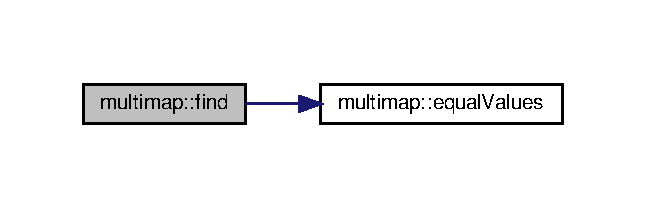
\includegraphics[width=310pt]{namespacemultimap_a3c5bc8037151780c38835c7f8a2f0722_cgraph}
\end{center}
\end{figure}
\mbox{\Hypertarget{namespacemultimap_ad8171701d0a623e4623721cb1743196c}\label{namespacemultimap_ad8171701d0a623e4623721cb1743196c}} 
\index{multimap@{multimap}!find@{find}}
\index{find@{find}!multimap@{multimap}}
\subsubsection{\texorpdfstring{find()}{find()}\hspace{0.1cm}{\footnotesize\ttfamily [4/4]}}
{\footnotesize\ttfamily template$<$typename type\+Multimap\+Key , typename type\+Multimap\+Value , typename type\+Key , typename type\+Value $>$ \\
std\+::multimap$<$type\+Multimap\+Key,type\+Multimap\+Value$>$\+::const\+\_\+iterator multimap\+::find (\begin{DoxyParamCaption}\item[{const std\+::multimap$<$ type\+Multimap\+Key, type\+Multimap\+Value $>$ \&}]{m,  }\item[{const type\+Key \&}]{first,  }\item[{const type\+Value \&}]{second,  }\item[{bool($\ast$)(const type\+Multimap\+Value \&, const type\+Value \&)}]{equal\+Values }\end{DoxyParamCaption})}

Find exact (key,value) pair in a multimap using comparator There must be an implicit type conversion between type\+Multimap\+Key and type\+Key There must be an implicit type conversion between type\+Multimap\+Value and type\+Value if using the default comparator 
\begin{DoxyParams}{Parameters}
{\em m} & \\
\hline
{\em first} & \\
\hline
{\em second} & \\
\hline
\end{DoxyParams}
\begin{DoxyReturn}{Returns}
an iterator to the first pair found or multimap\+::end() if not found 
\end{DoxyReturn}


Definition at line 139 of file multimap\+Utilities.\+h.



References equal\+Values().

Here is the call graph for this function\+:\nopagebreak
\begin{figure}[H]
\begin{center}
\leavevmode
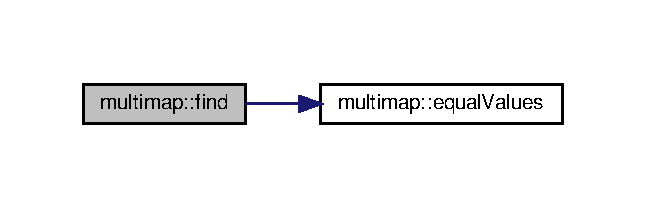
\includegraphics[width=310pt]{namespacemultimap_ad8171701d0a623e4623721cb1743196c_cgraph}
\end{center}
\end{figure}
\mbox{\Hypertarget{namespacemultimap_a1d03380ed2365e307412efab3c41731f}\label{namespacemultimap_a1d03380ed2365e307412efab3c41731f}} 
\index{multimap@{multimap}!keys@{keys}}
\index{keys@{keys}!multimap@{multimap}}
\subsubsection{\texorpdfstring{keys()}{keys()}}
{\footnotesize\ttfamily template$<$typename T , typename U $>$ \\
std\+::set$<$T$>$ multimap\+::keys (\begin{DoxyParamCaption}\item[{std\+::multimap$<$ T, U $>$ const \&}]{m }\end{DoxyParamCaption})}


\begin{DoxyParams}{Parameters}
{\em m} & \\
\hline
\end{DoxyParams}
\begin{DoxyReturn}{Returns}
the unique keys of a multimap 
\end{DoxyReturn}


Definition at line 33 of file multimap\+Utilities.\+h.

\mbox{\Hypertarget{namespacemultimap_a94c77f5e6ac9c4eaeb34a6c142b6ab0d}\label{namespacemultimap_a94c77f5e6ac9c4eaeb34a6c142b6ab0d}} 
\index{multimap@{multimap}!minimum\+Value@{minimum\+Value}}
\index{minimum\+Value@{minimum\+Value}!multimap@{multimap}}
\subsubsection{\texorpdfstring{minimum\+Value()}{minimumValue()}}
{\footnotesize\ttfamily template$<$typename T , typename U $>$ \\
std\+::multimap$<$T,U$>$\+::iterator\& multimap\+::minimum\+Value (\begin{DoxyParamCaption}\item[{std\+::multimap$<$ T, U $>$ \&}]{m,  }\item[{const T \&}]{key }\end{DoxyParamCaption})}

get the minimum value attributed to a given key 
\begin{DoxyParams}{Parameters}
{\em map} & \\
\hline
{\em key} & \\
\hline
\end{DoxyParams}
\begin{DoxyReturn}{Returns}
an iterator to the pair containing the minimum value or multimap\+::end() if not found 
\end{DoxyReturn}


Definition at line 168 of file multimap\+Utilities.\+h.

\mbox{\Hypertarget{namespacemultimap_aa170f94901a505969ecfa010c24f2877}\label{namespacemultimap_aa170f94901a505969ecfa010c24f2877}} 
\index{multimap@{multimap}!to\+String@{to\+String}}
\index{to\+String@{to\+String}!multimap@{multimap}}
\subsubsection{\texorpdfstring{to\+String()}{toString()}}
{\footnotesize\ttfamily template$<$typename T , typename U , typename std\+::enable\+\_\+if$<$ std\+::is\+\_\+fundamental$<$ T $>$\+::value \&\&std\+::is\+\_\+fundamental$<$ U $>$\+::value, T $>$\+::type  = 0$>$ \\
std\+::string multimap\+::to\+String (\begin{DoxyParamCaption}\item[{std\+::multimap$<$ T, U $>$ const \&}]{m,  }\item[{const \hyperlink{classStringFormatter}{String\+Formatter} \&}]{formater = {\ttfamily \hyperlink{stringFormatter_8h_abf1349c8e24162d0134072aff288f2a2}{default\+String\+Formatter}} }\end{DoxyParamCaption})}



Definition at line 151 of file multimap\+Utilities.\+h.



Referenced by Multimap\+Reversable$<$ T, U $>$\+::to\+String(), and Map\+Reversable$<$ type\+Vertex, type\+Community $>$\+::to\+String().

\mbox{\Hypertarget{namespacemultimap_a0b99e1d5a2730d58caee6e020509da9d}\label{namespacemultimap_a0b99e1d5a2730d58caee6e020509da9d}} 
\index{multimap@{multimap}!values@{values}}
\index{values@{values}!multimap@{multimap}}
\subsubsection{\texorpdfstring{values()}{values()}}
{\footnotesize\ttfamily template$<$typename T , typename U $>$ \\
std\+::set$<$T$>$ multimap\+::values (\begin{DoxyParamCaption}\item[{std\+::multimap$<$ T, U $>$ const \&}]{m }\end{DoxyParamCaption})}


\begin{DoxyParams}{Parameters}
{\em m} & \\
\hline
\end{DoxyParams}
\begin{DoxyReturn}{Returns}
the unique values of a multimap 
\end{DoxyReturn}


Definition at line 47 of file multimap\+Utilities.\+h.


\hypertarget{namespaceset}{}\section{set Namespace Reference}
\label{namespaceset}\index{set@{set}}
\subsection*{Functions}
\begin{DoxyCompactItemize}
\item 
{\footnotesize template$<$typename T , typename std\+::enable\+\_\+if$<$ std\+::is\+\_\+fundamental$<$ T $>$\+::value, T $>$\+::type  = 0$>$ }\\std\+::string \hyperlink{namespaceset_a61f35fff33becca4522a3f0a22ee8dfc}{to\+String} (std\+::set$<$ T $>$ const \&m)
\end{DoxyCompactItemize}


\subsection{Function Documentation}
\mbox{\Hypertarget{namespaceset_a61f35fff33becca4522a3f0a22ee8dfc}\label{namespaceset_a61f35fff33becca4522a3f0a22ee8dfc}} 
\index{set@{set}!to\+String@{to\+String}}
\index{to\+String@{to\+String}!set@{set}}
\subsubsection{\texorpdfstring{to\+String()}{toString()}}
{\footnotesize\ttfamily template$<$typename T , typename std\+::enable\+\_\+if$<$ std\+::is\+\_\+fundamental$<$ T $>$\+::value, T $>$\+::type  = 0$>$ \\
std\+::string set\+::to\+String (\begin{DoxyParamCaption}\item[{std\+::set$<$ T $>$ const \&}]{m }\end{DoxyParamCaption})}

Get the string representation of a set.


\begin{DoxyParams}{Parameters}
{\em m} & \\
\hline
\end{DoxyParams}
\begin{DoxyReturn}{Returns}
a string 
\end{DoxyReturn}


Definition at line 33 of file set\+Utilities.\+h.


\hypertarget{namespaceTime}{}\section{Time Namespace Reference}
\label{namespaceTime}\index{Time@{Time}}
\subsection*{Classes}
\begin{DoxyCompactItemize}
\item 
class \hyperlink{classTime_1_1TimeKeeper}{Time\+Keeper}
\begin{DoxyCompactList}\small\item\em Simple class used to keep track of elapsed time. \end{DoxyCompactList}\end{DoxyCompactItemize}
\subsection*{Functions}
\begin{DoxyCompactItemize}
\item 
\hyperlink{systemDefines_8h_abc0f5bc07737e498f287334775dff2b6}{uint64} \hyperlink{namespaceTime_a57ff57387f9a60589ccdbe9215843ffe}{long\+Time} (const timeval \&t)
\begin{DoxyCompactList}\small\item\em long\+Time Converts a timeval type time to an unsigned 64 bit integer \end{DoxyCompactList}\item 
\hyperlink{systemDefines_8h_abc0f5bc07737e498f287334775dff2b6}{uint64} \hyperlink{namespaceTime_a17419cc5dad406abf846351b1a75bd48}{long\+Time} (const timespec \&t)
\begin{DoxyCompactList}\small\item\em long\+Time Converts a timespec type time to an unsigned 64 bit integer \end{DoxyCompactList}\item 
\hyperlink{systemDefines_8h_abc0f5bc07737e498f287334775dff2b6}{uint64} \hyperlink{namespaceTime_ae414566445c9d392bb148cc98fe2cece}{current\+Time} ()
\begin{DoxyCompactList}\small\item\em Get the current system time in nanoseconds as an unsigned 64 bit integer. \end{DoxyCompactList}\end{DoxyCompactItemize}
\subsection*{Variables}
\begin{DoxyCompactItemize}
\item 
\hyperlink{classTime_1_1TimeKeeper}{Time\+Keeper} \hyperlink{namespaceTime_a321ca5eba84577aaaaeb2a79d28806c8}{time\+Keep}
\end{DoxyCompactItemize}


\subsection{Function Documentation}
\mbox{\Hypertarget{namespaceTime_ae414566445c9d392bb148cc98fe2cece}\label{namespaceTime_ae414566445c9d392bb148cc98fe2cece}} 
\index{Time@{Time}!current\+Time@{current\+Time}}
\index{current\+Time@{current\+Time}!Time@{Time}}
\subsubsection{\texorpdfstring{current\+Time()}{currentTime()}}
{\footnotesize\ttfamily \hyperlink{systemDefines_8h_abc0f5bc07737e498f287334775dff2b6}{uint64} Time\+::current\+Time (\begin{DoxyParamCaption}{ }\end{DoxyParamCaption})\hspace{0.3cm}{\ttfamily [inline]}}



Get the current system time in nanoseconds as an unsigned 64 bit integer. 

\begin{DoxyReturn}{Returns}
the current time or epoch (0) if an error occurred 
\end{DoxyReturn}


Definition at line 57 of file time\+Functions.\+h.



References long\+Time().



Referenced by Dyn\+Comm\+Base\+::add\+Remove\+Edges(), Time\+::\+Time\+Keeper\+::get(), and Time\+::\+Time\+Keeper\+::set().

Here is the call graph for this function\+:\nopagebreak
\begin{figure}[H]
\begin{center}
\leavevmode
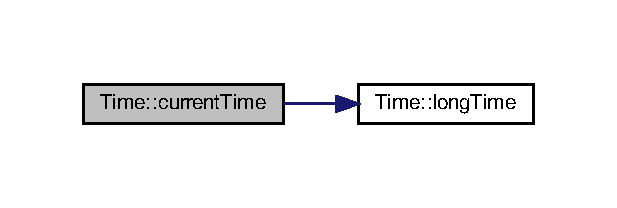
\includegraphics[width=296pt]{namespaceTime_ae414566445c9d392bb148cc98fe2cece_cgraph}
\end{center}
\end{figure}
\mbox{\Hypertarget{namespaceTime_a57ff57387f9a60589ccdbe9215843ffe}\label{namespaceTime_a57ff57387f9a60589ccdbe9215843ffe}} 
\index{Time@{Time}!long\+Time@{long\+Time}}
\index{long\+Time@{long\+Time}!Time@{Time}}
\subsubsection{\texorpdfstring{long\+Time()}{longTime()}\hspace{0.1cm}{\footnotesize\ttfamily [1/2]}}
{\footnotesize\ttfamily \hyperlink{systemDefines_8h_abc0f5bc07737e498f287334775dff2b6}{uint64} Time\+::long\+Time (\begin{DoxyParamCaption}\item[{const timeval \&}]{t }\end{DoxyParamCaption})\hspace{0.3cm}{\ttfamily [inline]}}



long\+Time Converts a timeval type time to an unsigned 64 bit integer 


\begin{DoxyParams}{Parameters}
{\em t} & is the timeval to convert \\
\hline
\end{DoxyParams}
\begin{DoxyReturn}{Returns}
an unsigned 64 bit integer representing time in nanoseconds 
\end{DoxyReturn}


Definition at line 33 of file time\+Functions.\+h.



Referenced by current\+Time().

\mbox{\Hypertarget{namespaceTime_a17419cc5dad406abf846351b1a75bd48}\label{namespaceTime_a17419cc5dad406abf846351b1a75bd48}} 
\index{Time@{Time}!long\+Time@{long\+Time}}
\index{long\+Time@{long\+Time}!Time@{Time}}
\subsubsection{\texorpdfstring{long\+Time()}{longTime()}\hspace{0.1cm}{\footnotesize\ttfamily [2/2]}}
{\footnotesize\ttfamily \hyperlink{systemDefines_8h_abc0f5bc07737e498f287334775dff2b6}{uint64} Time\+::long\+Time (\begin{DoxyParamCaption}\item[{const timespec \&}]{t }\end{DoxyParamCaption})\hspace{0.3cm}{\ttfamily [inline]}}



long\+Time Converts a timespec type time to an unsigned 64 bit integer 


\begin{DoxyParams}{Parameters}
{\em t} & is the timespec to convert \\
\hline
\end{DoxyParams}
\begin{DoxyReturn}{Returns}
an unsigned 64 bit integer representing time in nanoseconds 
\end{DoxyReturn}


Definition at line 46 of file time\+Functions.\+h.



\subsection{Variable Documentation}
\mbox{\Hypertarget{namespaceTime_a321ca5eba84577aaaaeb2a79d28806c8}\label{namespaceTime_a321ca5eba84577aaaaeb2a79d28806c8}} 
\index{Time@{Time}!time\+Keep@{time\+Keep}}
\index{time\+Keep@{time\+Keep}!Time@{Time}}
\subsubsection{\texorpdfstring{time\+Keep}{timeKeep}}
{\footnotesize\ttfamily \hyperlink{classTime_1_1TimeKeeper}{Time\+Keeper} Time\+::time\+Keep}



Definition at line 146 of file time\+Functions.\+h.


\chapter{Class Documentation}
\hypertarget{classAlgorithm}{}\section{Algorithm Class Reference}
\label{classAlgorithm}\index{Algorithm@{Algorithm}}


Aggregator class for all main algorithms.  




{\ttfamily \#include $<$algorithm.\+h$>$}



Inheritance diagram for Algorithm\+:
\nopagebreak
\begin{figure}[H]
\begin{center}
\leavevmode
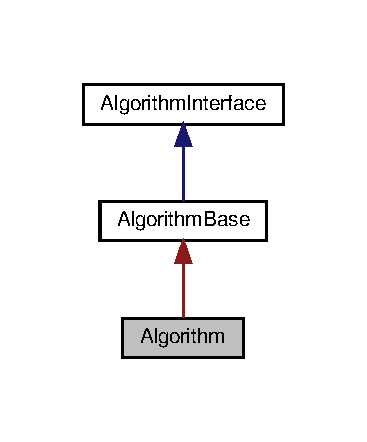
\includegraphics[width=176pt]{classAlgorithm__inherit__graph}
\end{center}
\end{figure}


Collaboration diagram for Algorithm\+:
\nopagebreak
\begin{figure}[H]
\begin{center}
\leavevmode
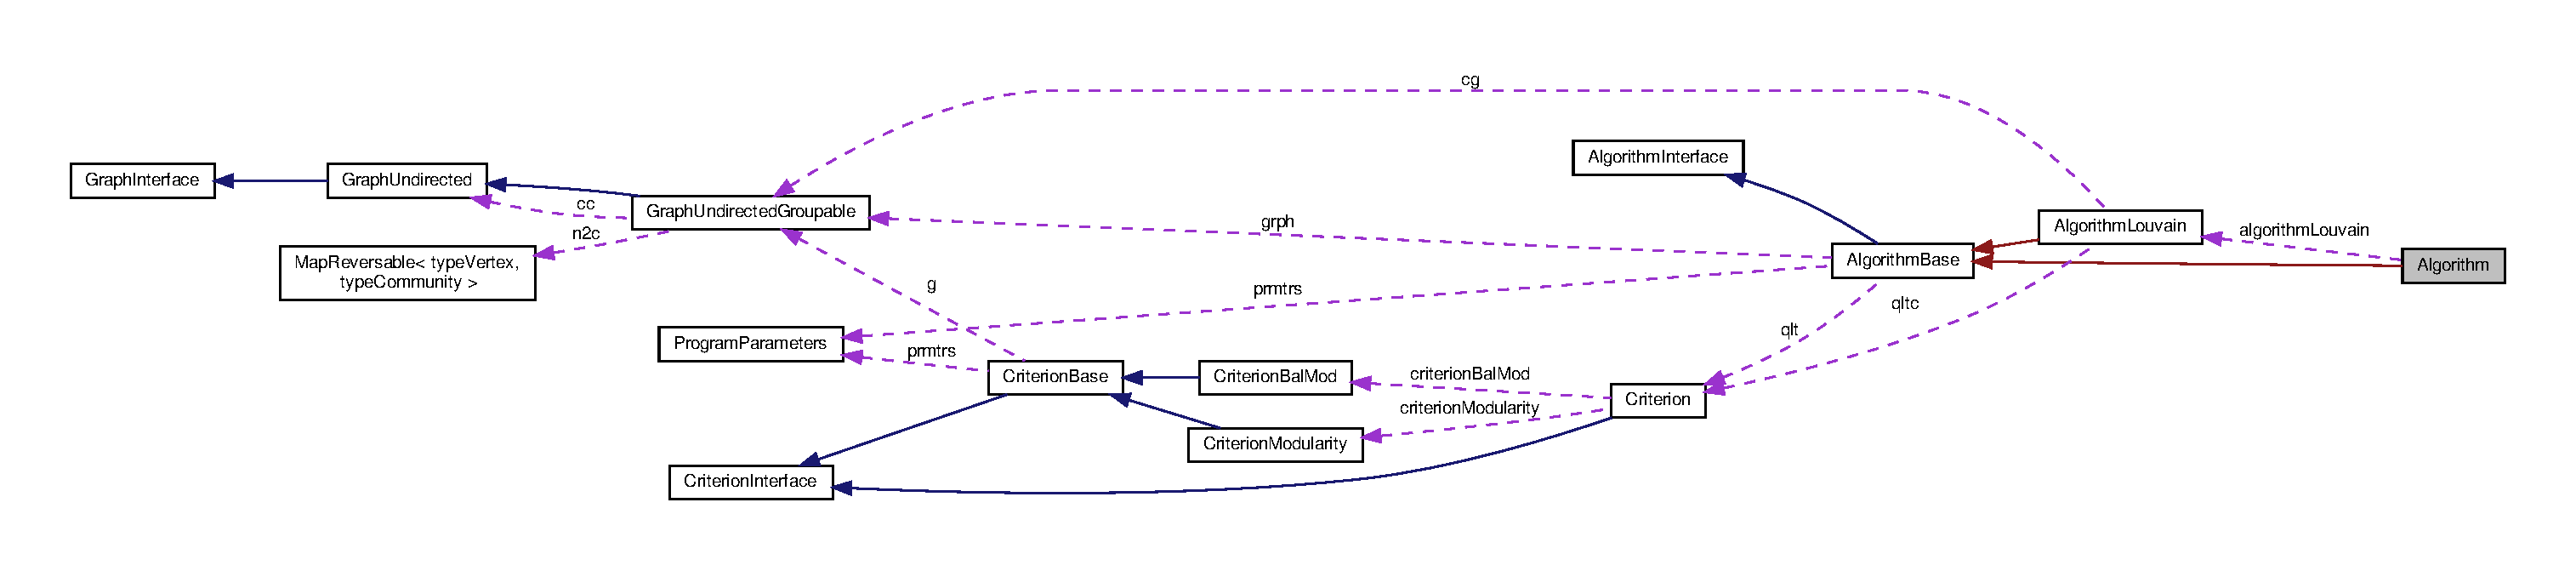
\includegraphics[width=350pt]{classAlgorithm__coll__graph}
\end{center}
\end{figure}
\subsection*{Public Types}
\begin{DoxyCompactItemize}
\item 
enum \hyperlink{classAlgorithm_a38e19a8c3dc51b97563a34d9e59a748d}{A\+L\+G\+O\+R\+I\+T\+HM} \+: unsigned int \{ \hyperlink{classAlgorithm_a38e19a8c3dc51b97563a34d9e59a748dab77e66715d6be972cdbf6cc4d990e732}{A\+L\+G\+O\+R\+I\+T\+H\+M\+::\+L\+O\+U\+V\+A\+IN} =1, 
\hyperlink{classAlgorithm_a38e19a8c3dc51b97563a34d9e59a748da1081b2130037a7b464f64d6cc82b3100}{A\+L\+G\+O\+R\+I\+T\+H\+M\+::\+S\+H\+A\+K\+EN}
 \}
\end{DoxyCompactItemize}
\subsection*{Public Member Functions}
\begin{DoxyCompactItemize}
\item 
\hyperlink{classAlgorithm_adb63a5f03ed70abb7e355631799c1ad0}{Algorithm} ()=delete
\item 
\hyperlink{classAlgorithm_a1a77fee87ecd410f2fae6db4c246c3ab}{Algorithm} (\hyperlink{classGraphUndirectedGroupable}{Graph\+Undirected\+Groupable} \&\hyperlink{classAlgorithmBase_a54b71b720b025291d9802e20874c860d}{grph}, \hyperlink{classCriterion}{Criterion} \&quality, \hyperlink{classAlgorithm_a38e19a8c3dc51b97563a34d9e59a748d}{A\+L\+G\+O\+R\+I\+T\+HM} algorithm=\hyperlink{classAlgorithm_a38e19a8c3dc51b97563a34d9e59a748dab77e66715d6be972cdbf6cc4d990e732}{A\+L\+G\+O\+R\+I\+T\+H\+M\+::\+L\+O\+U\+V\+A\+IN}, \hyperlink{structProgramParameters}{Program\+Parameters} \&algorithm\+Parameters=\hyperlink{program_8h_ae2d819404495f80f31db7676c1329d19}{arguments\+Default})
\item 
bool \hyperlink{classAlgorithm_a8ec65e07ed59a0f8b8491683b95626d2}{add\+Remove\+Edges} (\hyperlink{classReaderInterface}{Reader\+Interface}$<$ \hyperlink{classEdge}{Edge} $>$ $\ast$reader)
\item 
const std\+::string \hyperlink{classAlgorithm_a3b3172af613b02bfb1dc2502553d91c0}{to\+String} (const \hyperlink{classStringFormatter}{String\+Formatter} \&sf=\hyperlink{stringFormatter_8h_abf1349c8e24162d0134072aff288f2a2}{default\+String\+Formatter}) const
\end{DoxyCompactItemize}
\subsection*{Private Member Functions}
\begin{DoxyCompactItemize}
\item 
bool \hyperlink{classAlgorithm_a5835b23797b9d00f4090b996660af5d4}{add\+Remove\+Edge\+Pre} (const \hyperlink{edge_8h_a5fbd20c46956d479cb10afc9855223f6}{type\+Vertex} \&source, const \hyperlink{edge_8h_a5fbd20c46956d479cb10afc9855223f6}{type\+Vertex} \&destination, const \hyperlink{edge_8h_a2e7ea3be891ac8b52f749ec73fee6dd2}{type\+Weight} \&weight=1.\+0)
\item 
bool \hyperlink{classAlgorithm_ad78e2c5819da723c373ce6d4a28ac36d}{add\+Remove\+Edge\+Post} (const \hyperlink{edge_8h_a5fbd20c46956d479cb10afc9855223f6}{type\+Vertex} \&source, const \hyperlink{edge_8h_a5fbd20c46956d479cb10afc9855223f6}{type\+Vertex} \&destination, const \hyperlink{edge_8h_a2e7ea3be891ac8b52f749ec73fee6dd2}{type\+Weight} \&weight=1.\+0)
\item 
bool \hyperlink{classAlgorithm_a10dcb6b63ba40fad0bf11a0fef7b40f5}{run} ()
\end{DoxyCompactItemize}
\subsection*{Private Attributes}
\begin{DoxyCompactItemize}
\item 
const \hyperlink{classAlgorithm_a38e19a8c3dc51b97563a34d9e59a748d}{A\+L\+G\+O\+R\+I\+T\+HM} \hyperlink{classAlgorithm_aaee2fd7b239cc8721ec894716271dcd9}{algrthm}
\item 
\hyperlink{classAlgorithmLouvain}{Algorithm\+Louvain} \hyperlink{classAlgorithm_a95ef62342279e55525eacf34e83bc2ca}{algorithm\+Louvain}
\end{DoxyCompactItemize}


\subsection{Detailed Description}
Aggregator class for all main algorithms. 

It is a simple class that only instantiates all algorithms and dispatches function calls to the correct one.

\begin{DoxyAuthor}{Author}
poltergeist0
\end{DoxyAuthor}
\begin{DoxyDate}{Date}
2019-\/01-\/01 
\end{DoxyDate}


Definition at line 63 of file algorithm.\+h.



\subsection{Member Enumeration Documentation}
\mbox{\Hypertarget{classAlgorithm_a38e19a8c3dc51b97563a34d9e59a748d}\label{classAlgorithm_a38e19a8c3dc51b97563a34d9e59a748d}} 
\index{Algorithm@{Algorithm}!A\+L\+G\+O\+R\+I\+T\+HM@{A\+L\+G\+O\+R\+I\+T\+HM}}
\index{A\+L\+G\+O\+R\+I\+T\+HM@{A\+L\+G\+O\+R\+I\+T\+HM}!Algorithm@{Algorithm}}
\subsubsection{\texorpdfstring{A\+L\+G\+O\+R\+I\+T\+HM}{ALGORITHM}}
{\footnotesize\ttfamily enum \hyperlink{classAlgorithm_a38e19a8c3dc51b97563a34d9e59a748d}{Algorithm\+::\+A\+L\+G\+O\+R\+I\+T\+HM} \+: unsigned int\hspace{0.3cm}{\ttfamily [strong]}}

Enumeration with the list of supported Dynamic Communities algorithms. This enumeration must start at 1 since this code is used in R and R indexing (for arrays, etc) starts at 1 instead of 0. Otherwise C++ would assign the first algorithm a 0. \begin{DoxyEnumFields}{Enumerator}
\raisebox{\heightof{T}}[0pt][0pt]{\index{L\+O\+U\+V\+A\+IN@{L\+O\+U\+V\+A\+IN}!Algorithm@{Algorithm}}\index{Algorithm@{Algorithm}!L\+O\+U\+V\+A\+IN@{L\+O\+U\+V\+A\+IN}}}\mbox{\Hypertarget{classAlgorithm_a38e19a8c3dc51b97563a34d9e59a748dab77e66715d6be972cdbf6cc4d990e732}\label{classAlgorithm_a38e19a8c3dc51b97563a34d9e59a748dab77e66715d6be972cdbf6cc4d990e732}} 
L\+O\+U\+V\+A\+IN&\\
\hline

\raisebox{\heightof{T}}[0pt][0pt]{\index{S\+H\+A\+K\+EN@{S\+H\+A\+K\+EN}!Algorithm@{Algorithm}}\index{Algorithm@{Algorithm}!S\+H\+A\+K\+EN@{S\+H\+A\+K\+EN}}}\mbox{\Hypertarget{classAlgorithm_a38e19a8c3dc51b97563a34d9e59a748da1081b2130037a7b464f64d6cc82b3100}\label{classAlgorithm_a38e19a8c3dc51b97563a34d9e59a748da1081b2130037a7b464f64d6cc82b3100}} 
S\+H\+A\+K\+EN&\\
\hline

\end{DoxyEnumFields}


Definition at line 76 of file algorithm.\+h.



\subsection{Constructor \& Destructor Documentation}
\mbox{\Hypertarget{classAlgorithm_adb63a5f03ed70abb7e355631799c1ad0}\label{classAlgorithm_adb63a5f03ed70abb7e355631799c1ad0}} 
\index{Algorithm@{Algorithm}!Algorithm@{Algorithm}}
\index{Algorithm@{Algorithm}!Algorithm@{Algorithm}}
\subsubsection{\texorpdfstring{Algorithm()}{Algorithm()}\hspace{0.1cm}{\footnotesize\ttfamily [1/2]}}
{\footnotesize\ttfamily Algorithm\+::\+Algorithm (\begin{DoxyParamCaption}{ }\end{DoxyParamCaption})\hspace{0.3cm}{\ttfamily [delete]}}

Default constructor not acceptable. Must be passed at least the chosen algorithm and the graph 

Referenced by run().

\mbox{\Hypertarget{classAlgorithm_a1a77fee87ecd410f2fae6db4c246c3ab}\label{classAlgorithm_a1a77fee87ecd410f2fae6db4c246c3ab}} 
\index{Algorithm@{Algorithm}!Algorithm@{Algorithm}}
\index{Algorithm@{Algorithm}!Algorithm@{Algorithm}}
\subsubsection{\texorpdfstring{Algorithm()}{Algorithm()}\hspace{0.1cm}{\footnotesize\ttfamily [2/2]}}
{\footnotesize\ttfamily Algorithm\+::\+Algorithm (\begin{DoxyParamCaption}\item[{\hyperlink{classGraphUndirectedGroupable}{Graph\+Undirected\+Groupable} \&}]{grph,  }\item[{\hyperlink{classCriterion}{Criterion} \&}]{quality,  }\item[{\hyperlink{classAlgorithm_a38e19a8c3dc51b97563a34d9e59a748d}{A\+L\+G\+O\+R\+I\+T\+HM}}]{algorithm = {\ttfamily \hyperlink{classAlgorithm_a38e19a8c3dc51b97563a34d9e59a748dab77e66715d6be972cdbf6cc4d990e732}{A\+L\+G\+O\+R\+I\+T\+H\+M\+::\+L\+O\+U\+V\+A\+IN}},  }\item[{\hyperlink{structProgramParameters}{Program\+Parameters} \&}]{algorithm\+Parameters = {\ttfamily \hyperlink{program_8h_ae2d819404495f80f31db7676c1329d19}{arguments\+Default}} }\end{DoxyParamCaption})\hspace{0.3cm}{\ttfamily [inline]}}

Constructor.


\begin{DoxyParams}{Parameters}
{\em graph} & reference to the graph object \\
\hline
{\em quality} & reference to the quality object \\
\hline
{\em algorithm\+Parameters} & reference to the parameters object \\
\hline
\end{DoxyParams}


Definition at line 196 of file algorithm.\+h.



\subsection{Member Function Documentation}
\mbox{\Hypertarget{classAlgorithm_ad78e2c5819da723c373ce6d4a28ac36d}\label{classAlgorithm_ad78e2c5819da723c373ce6d4a28ac36d}} 
\index{Algorithm@{Algorithm}!add\+Remove\+Edge\+Post@{add\+Remove\+Edge\+Post}}
\index{add\+Remove\+Edge\+Post@{add\+Remove\+Edge\+Post}!Algorithm@{Algorithm}}
\subsubsection{\texorpdfstring{add\+Remove\+Edge\+Post()}{addRemoveEdgePost()}}
{\footnotesize\ttfamily bool Algorithm\+::add\+Remove\+Edge\+Post (\begin{DoxyParamCaption}\item[{const \hyperlink{edge_8h_a5fbd20c46956d479cb10afc9855223f6}{type\+Vertex} \&}]{source,  }\item[{const \hyperlink{edge_8h_a5fbd20c46956d479cb10afc9855223f6}{type\+Vertex} \&}]{destination,  }\item[{const \hyperlink{edge_8h_a2e7ea3be891ac8b52f749ec73fee6dd2}{type\+Weight} \&}]{weight = {\ttfamily 1.0} }\end{DoxyParamCaption})\hspace{0.3cm}{\ttfamily [inline]}, {\ttfamily [private]}, {\ttfamily [virtual]}}

Function execute after adding or removing a single edge from the graph. It is used internally by the add\+Remove\+Edges function. Useful if post-\/processing is required, for example, to update some of variables after the edge has be added or removed. Any edge with a weight different from zero is inserted. Any edge with a weight of exactly zero is removed. Redirects call to algorithm variable.


\begin{DoxyParams}{Parameters}
{\em source} & source vertex \\
\hline
{\em destination} & destination vertex \\
\hline
{\em weight} & optional if adding an edge. Must be exactly zero to remove an edge. \\
\hline
\end{DoxyParams}
\begin{DoxyReturn}{Returns}
true if all operations succeeded. False, otherwise. 
\end{DoxyReturn}


Implements \hyperlink{classAlgorithmInterface_ac97ed4df4fd2b14b16d55c1b3b9749b6}{Algorithm\+Interface}.



Definition at line 141 of file algorithm.\+h.



References Algorithm\+Louvain\+::add\+Remove\+Edge\+Post(), and L\+O\+U\+V\+A\+IN.



Referenced by add\+Remove\+Edges().

Here is the call graph for this function\+:
\nopagebreak
\begin{figure}[H]
\begin{center}
\leavevmode
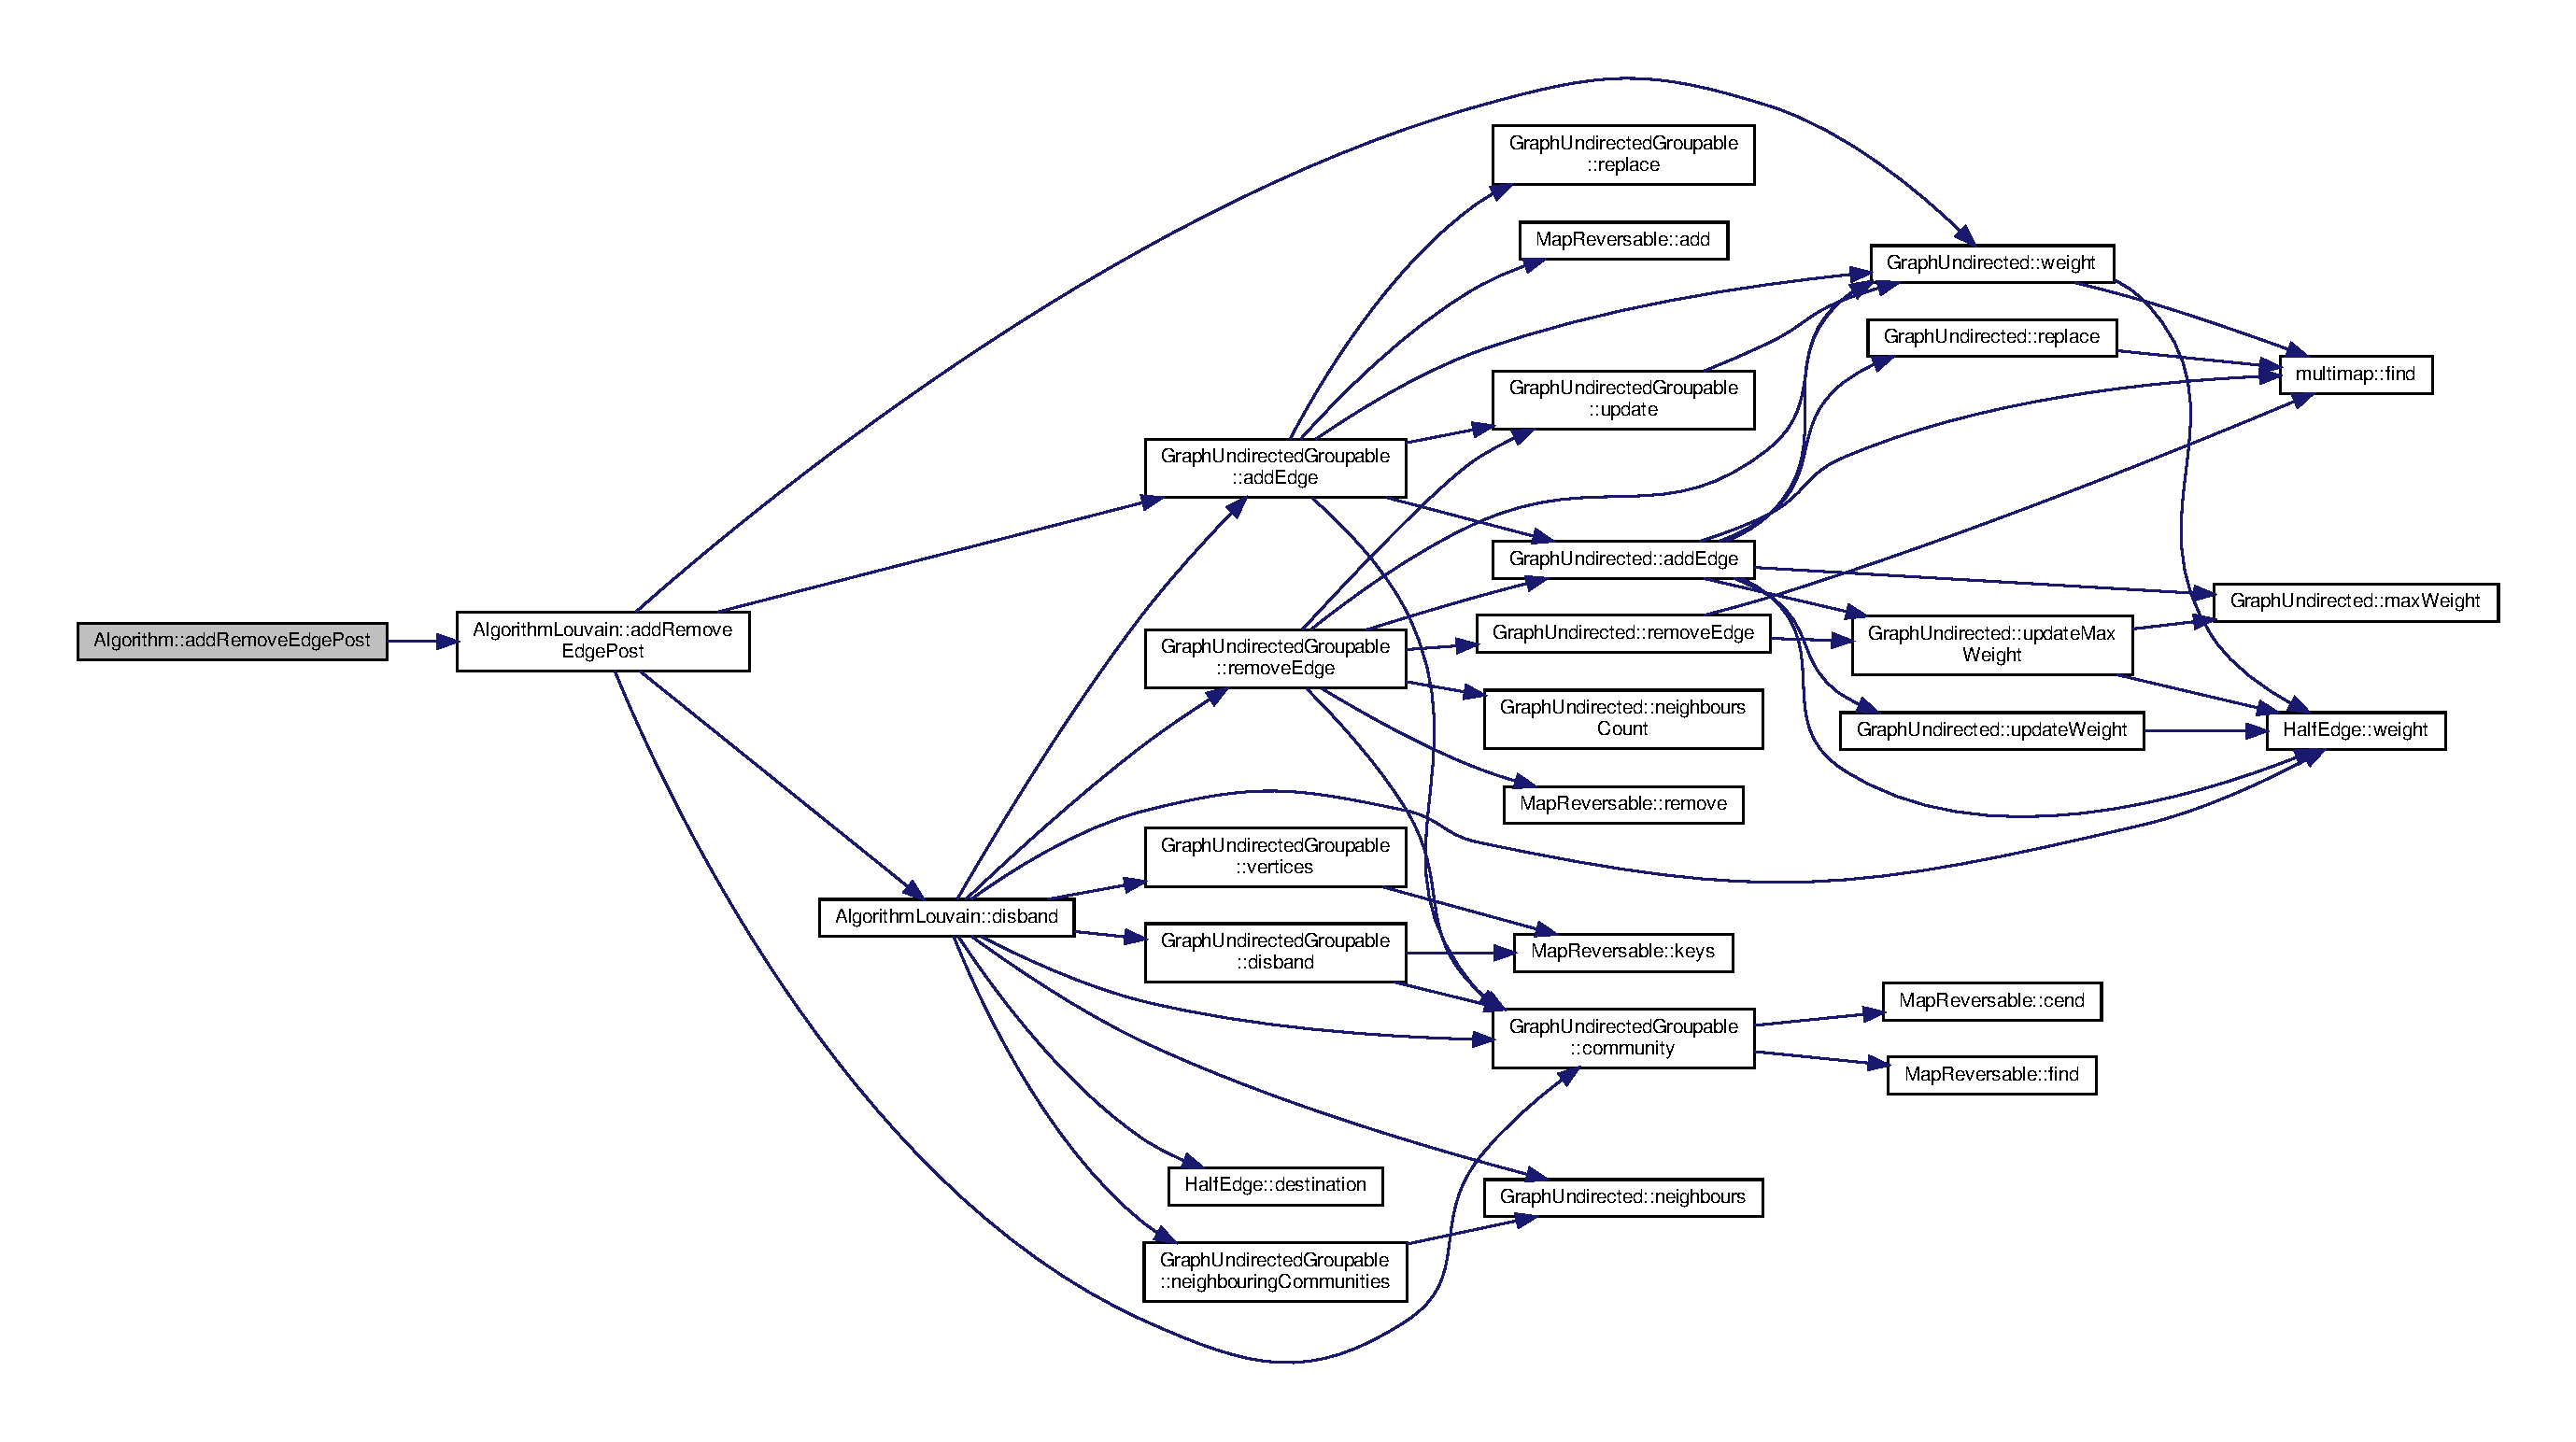
\includegraphics[width=350pt]{classAlgorithm_ad78e2c5819da723c373ce6d4a28ac36d_cgraph}
\end{center}
\end{figure}
\mbox{\Hypertarget{classAlgorithm_a5835b23797b9d00f4090b996660af5d4}\label{classAlgorithm_a5835b23797b9d00f4090b996660af5d4}} 
\index{Algorithm@{Algorithm}!add\+Remove\+Edge\+Pre@{add\+Remove\+Edge\+Pre}}
\index{add\+Remove\+Edge\+Pre@{add\+Remove\+Edge\+Pre}!Algorithm@{Algorithm}}
\subsubsection{\texorpdfstring{add\+Remove\+Edge\+Pre()}{addRemoveEdgePre()}}
{\footnotesize\ttfamily bool Algorithm\+::add\+Remove\+Edge\+Pre (\begin{DoxyParamCaption}\item[{const \hyperlink{edge_8h_a5fbd20c46956d479cb10afc9855223f6}{type\+Vertex} \&}]{source,  }\item[{const \hyperlink{edge_8h_a5fbd20c46956d479cb10afc9855223f6}{type\+Vertex} \&}]{destination,  }\item[{const \hyperlink{edge_8h_a2e7ea3be891ac8b52f749ec73fee6dd2}{type\+Weight} \&}]{weight = {\ttfamily 1.0} }\end{DoxyParamCaption})\hspace{0.3cm}{\ttfamily [inline]}, {\ttfamily [private]}, {\ttfamily [virtual]}}

Function to execute before adding or removing a single edge from the graph. It is used internally by the add\+Remove\+Edges function. Useful if pre-\/processing is required, for example, to update some of variables before the edge can be added or removed. Any edge with a weight different from zero is inserted. Any edge with a weight of exactly zero is removed. Redirects call to algorithm variable.


\begin{DoxyParams}{Parameters}
{\em source} & source vertex \\
\hline
{\em destination} & destination vertex \\
\hline
{\em weight} & optional if adding an edge. Must be exactly zero to remove an edge. \\
\hline
\end{DoxyParams}
\begin{DoxyReturn}{Returns}
true if all operations succeeded. False, otherwise. 
\end{DoxyReturn}


Implements \hyperlink{classAlgorithmInterface_ae5a6e84b139768dff92a70cacaec7472}{Algorithm\+Interface}.



Definition at line 110 of file algorithm.\+h.



References Algorithm\+Louvain\+::add\+Remove\+Edge\+Pre(), and L\+O\+U\+V\+A\+IN.



Referenced by add\+Remove\+Edges().

Here is the call graph for this function\+:
\nopagebreak
\begin{figure}[H]
\begin{center}
\leavevmode
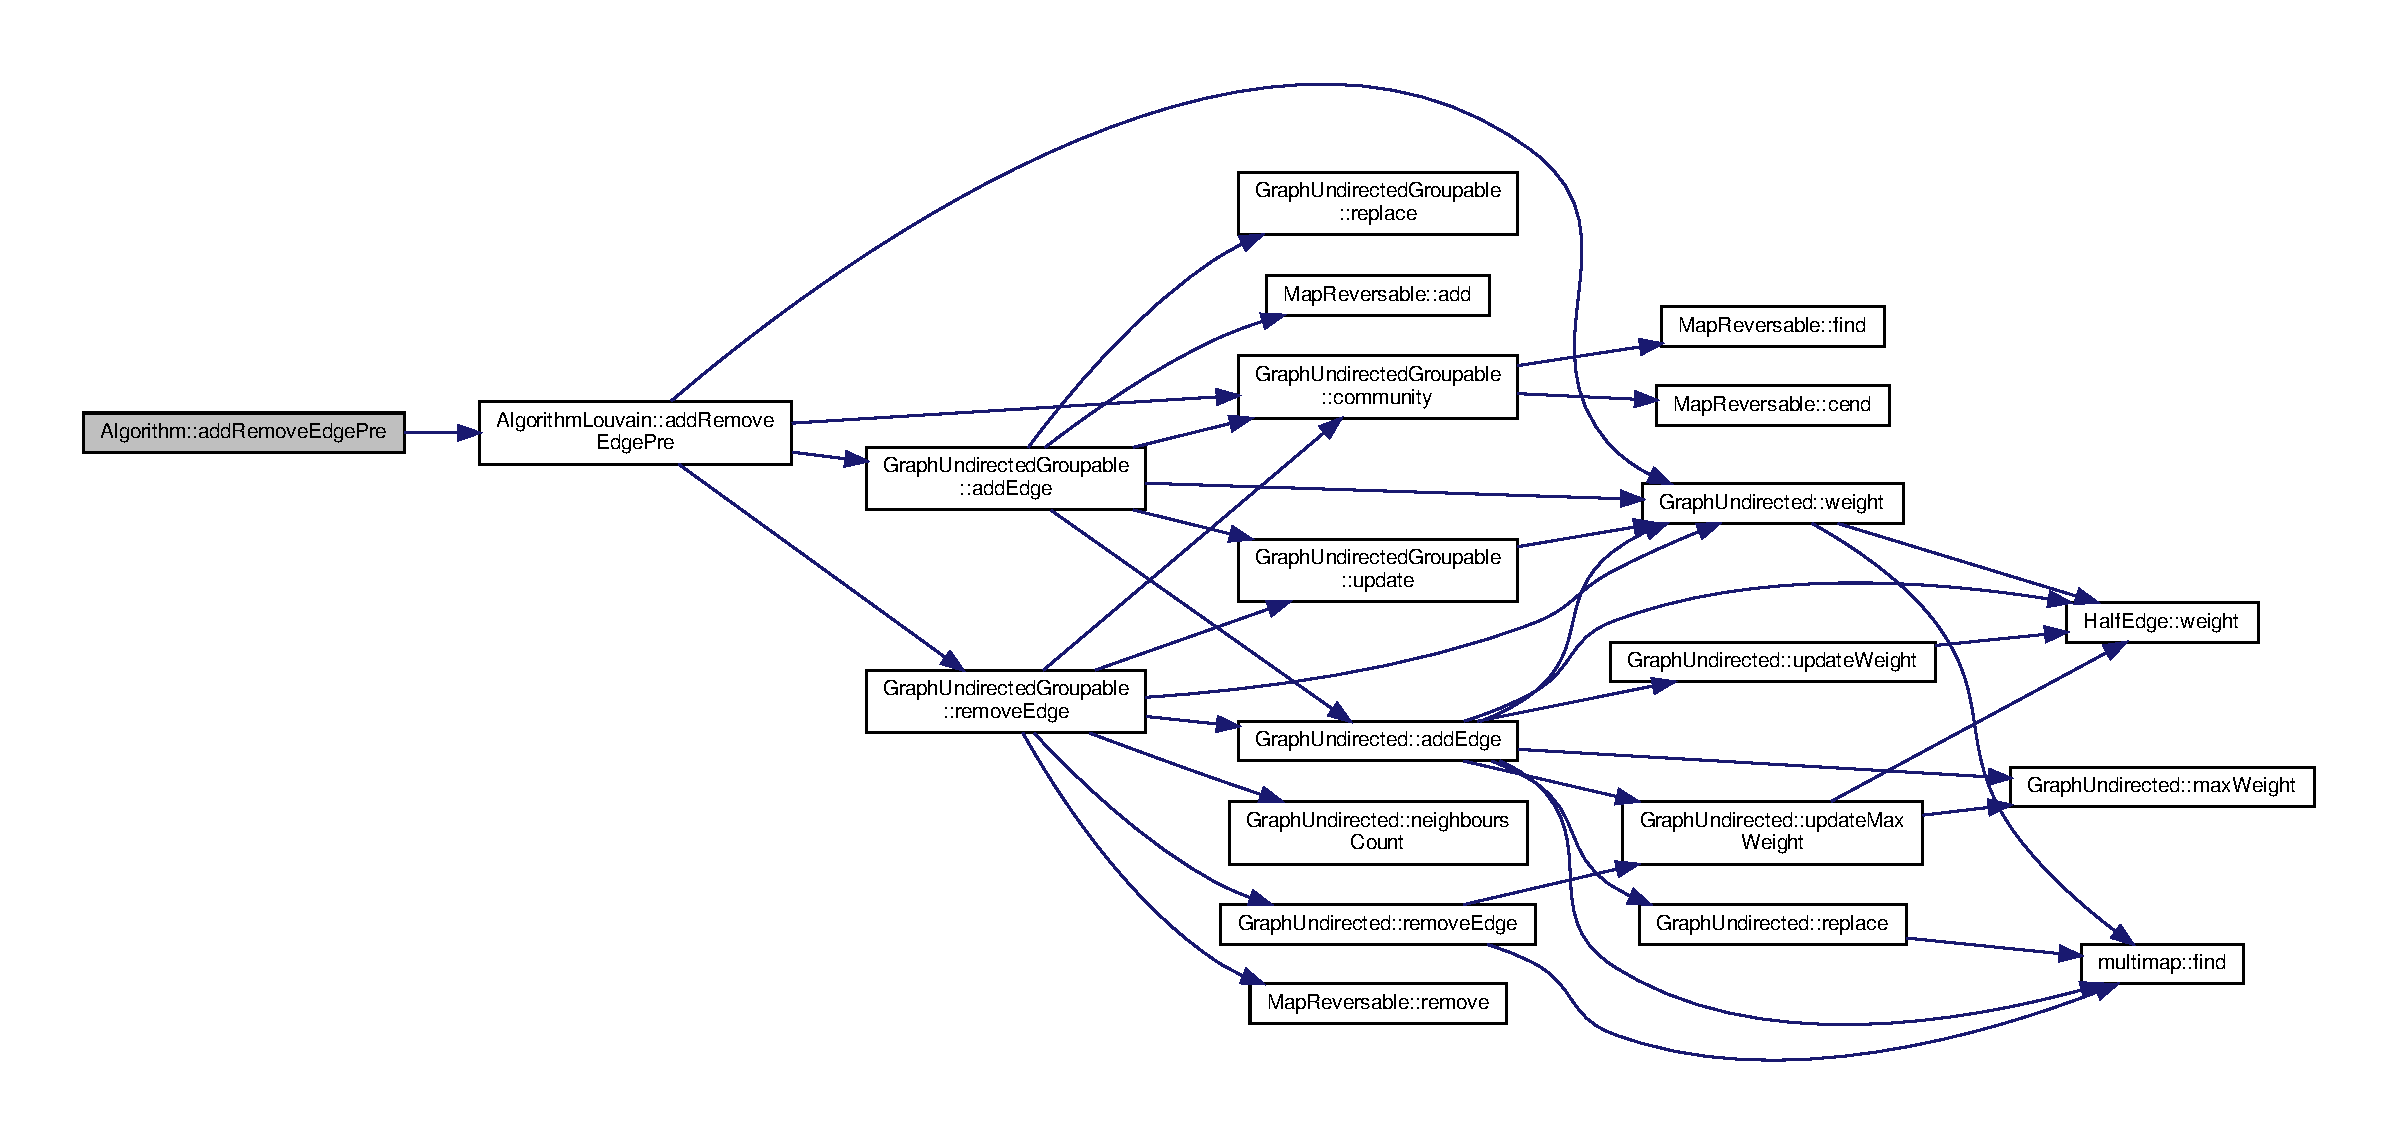
\includegraphics[width=350pt]{classAlgorithm_a5835b23797b9d00f4090b996660af5d4_cgraph}
\end{center}
\end{figure}
\mbox{\Hypertarget{classAlgorithm_a8ec65e07ed59a0f8b8491683b95626d2}\label{classAlgorithm_a8ec65e07ed59a0f8b8491683b95626d2}} 
\index{Algorithm@{Algorithm}!add\+Remove\+Edges@{add\+Remove\+Edges}}
\index{add\+Remove\+Edges@{add\+Remove\+Edges}!Algorithm@{Algorithm}}
\subsubsection{\texorpdfstring{add\+Remove\+Edges()}{addRemoveEdges()}}
{\footnotesize\ttfamily bool Algorithm\+::add\+Remove\+Edges (\begin{DoxyParamCaption}\item[{\hyperlink{classReaderInterface}{Reader\+Interface}$<$ \hyperlink{classEdge}{Edge} $>$ $\ast$}]{reader }\end{DoxyParamCaption})\hspace{0.3cm}{\ttfamily [inline]}}

Function to add and remove edges from the graph. Any edge with a weight different from zero is inserted. Any edge with a weight of exactly zero is removed.


\begin{DoxyParams}{Parameters}
{\em reader} & is a Reader object that is responsible for converting the required data from its original format to Edges \\
\hline
\end{DoxyParams}
\begin{DoxyReturn}{Returns}
true if adding/removing succeeded 
\end{DoxyReturn}


Definition at line 223 of file algorithm.\+h.



References Graph\+Undirected\+Groupable\+::add\+Edge(), add\+Remove\+Edge\+Post(), add\+Remove\+Edge\+Pre(), Edge\+::destination(), Algorithm\+Base\+::grph, Reader\+Interface$<$ T\+Y\+P\+E\+R\+E\+T\+U\+R\+N $>$\+::has\+Next(), Reader\+Interface$<$ T\+Y\+P\+E\+R\+E\+T\+U\+R\+N $>$\+::next(), Graph\+Undirected\+Groupable\+::remove\+Edge(), run(), Edge\+::source(), and Edge\+::weight().



Referenced by Dyn\+Comm\+Base\+::add\+Remove\+Edges().

Here is the call graph for this function\+:
\nopagebreak
\begin{figure}[H]
\begin{center}
\leavevmode
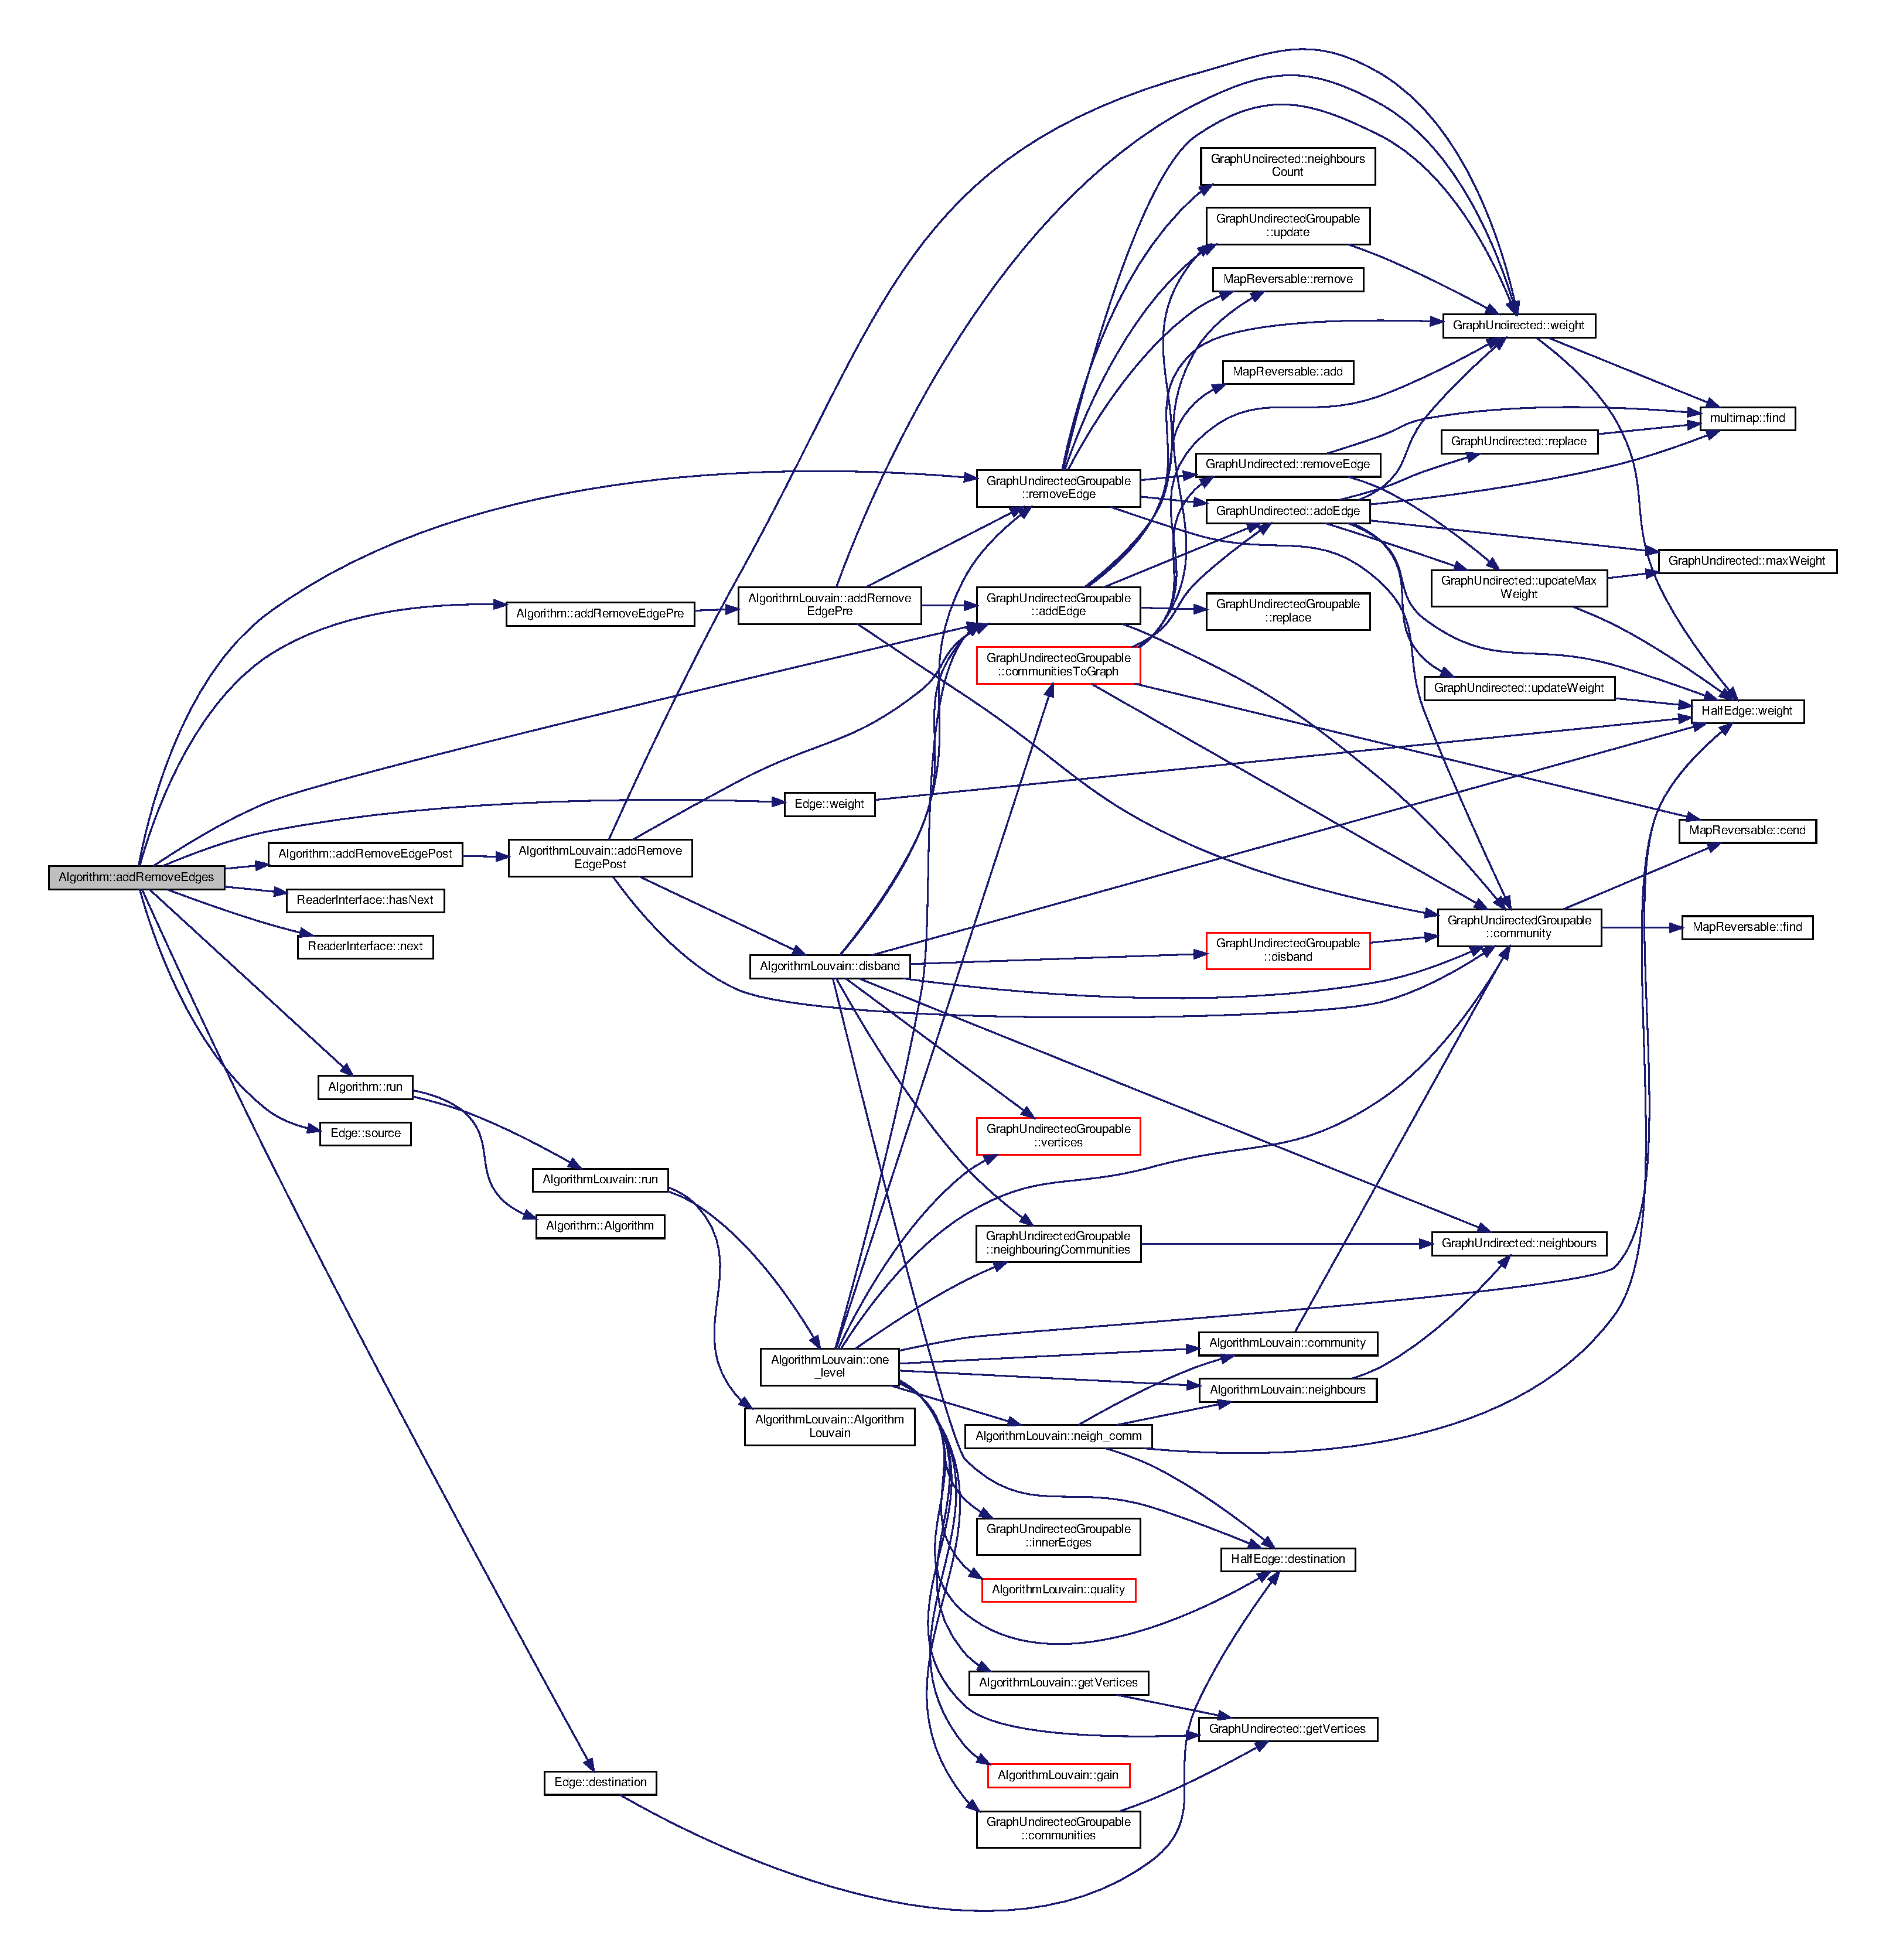
\includegraphics[width=350pt]{classAlgorithm_a8ec65e07ed59a0f8b8491683b95626d2_cgraph}
\end{center}
\end{figure}
\mbox{\Hypertarget{classAlgorithm_a10dcb6b63ba40fad0bf11a0fef7b40f5}\label{classAlgorithm_a10dcb6b63ba40fad0bf11a0fef7b40f5}} 
\index{Algorithm@{Algorithm}!run@{run}}
\index{run@{run}!Algorithm@{Algorithm}}
\subsubsection{\texorpdfstring{run()}{run()}}
{\footnotesize\ttfamily bool Algorithm\+::run (\begin{DoxyParamCaption}{ }\end{DoxyParamCaption})\hspace{0.3cm}{\ttfamily [inline]}, {\ttfamily [private]}, {\ttfamily [virtual]}}

Function where the actual algorithms are implemented. It is called at the end of the add\+Remove\+Edges function. Redirects call to algorithm variable.

\begin{DoxyReturn}{Returns}
true if all operations succeeded. False, otherwise. 
\end{DoxyReturn}


Implements \hyperlink{classAlgorithmInterface_a0bafcdabd2b5fd45abe97af91e02ca14}{Algorithm\+Interface}.



Definition at line 165 of file algorithm.\+h.



References Algorithm(), L\+O\+U\+V\+A\+IN, and Algorithm\+Louvain\+::run().



Referenced by add\+Remove\+Edges().

Here is the call graph for this function\+:
\nopagebreak
\begin{figure}[H]
\begin{center}
\leavevmode
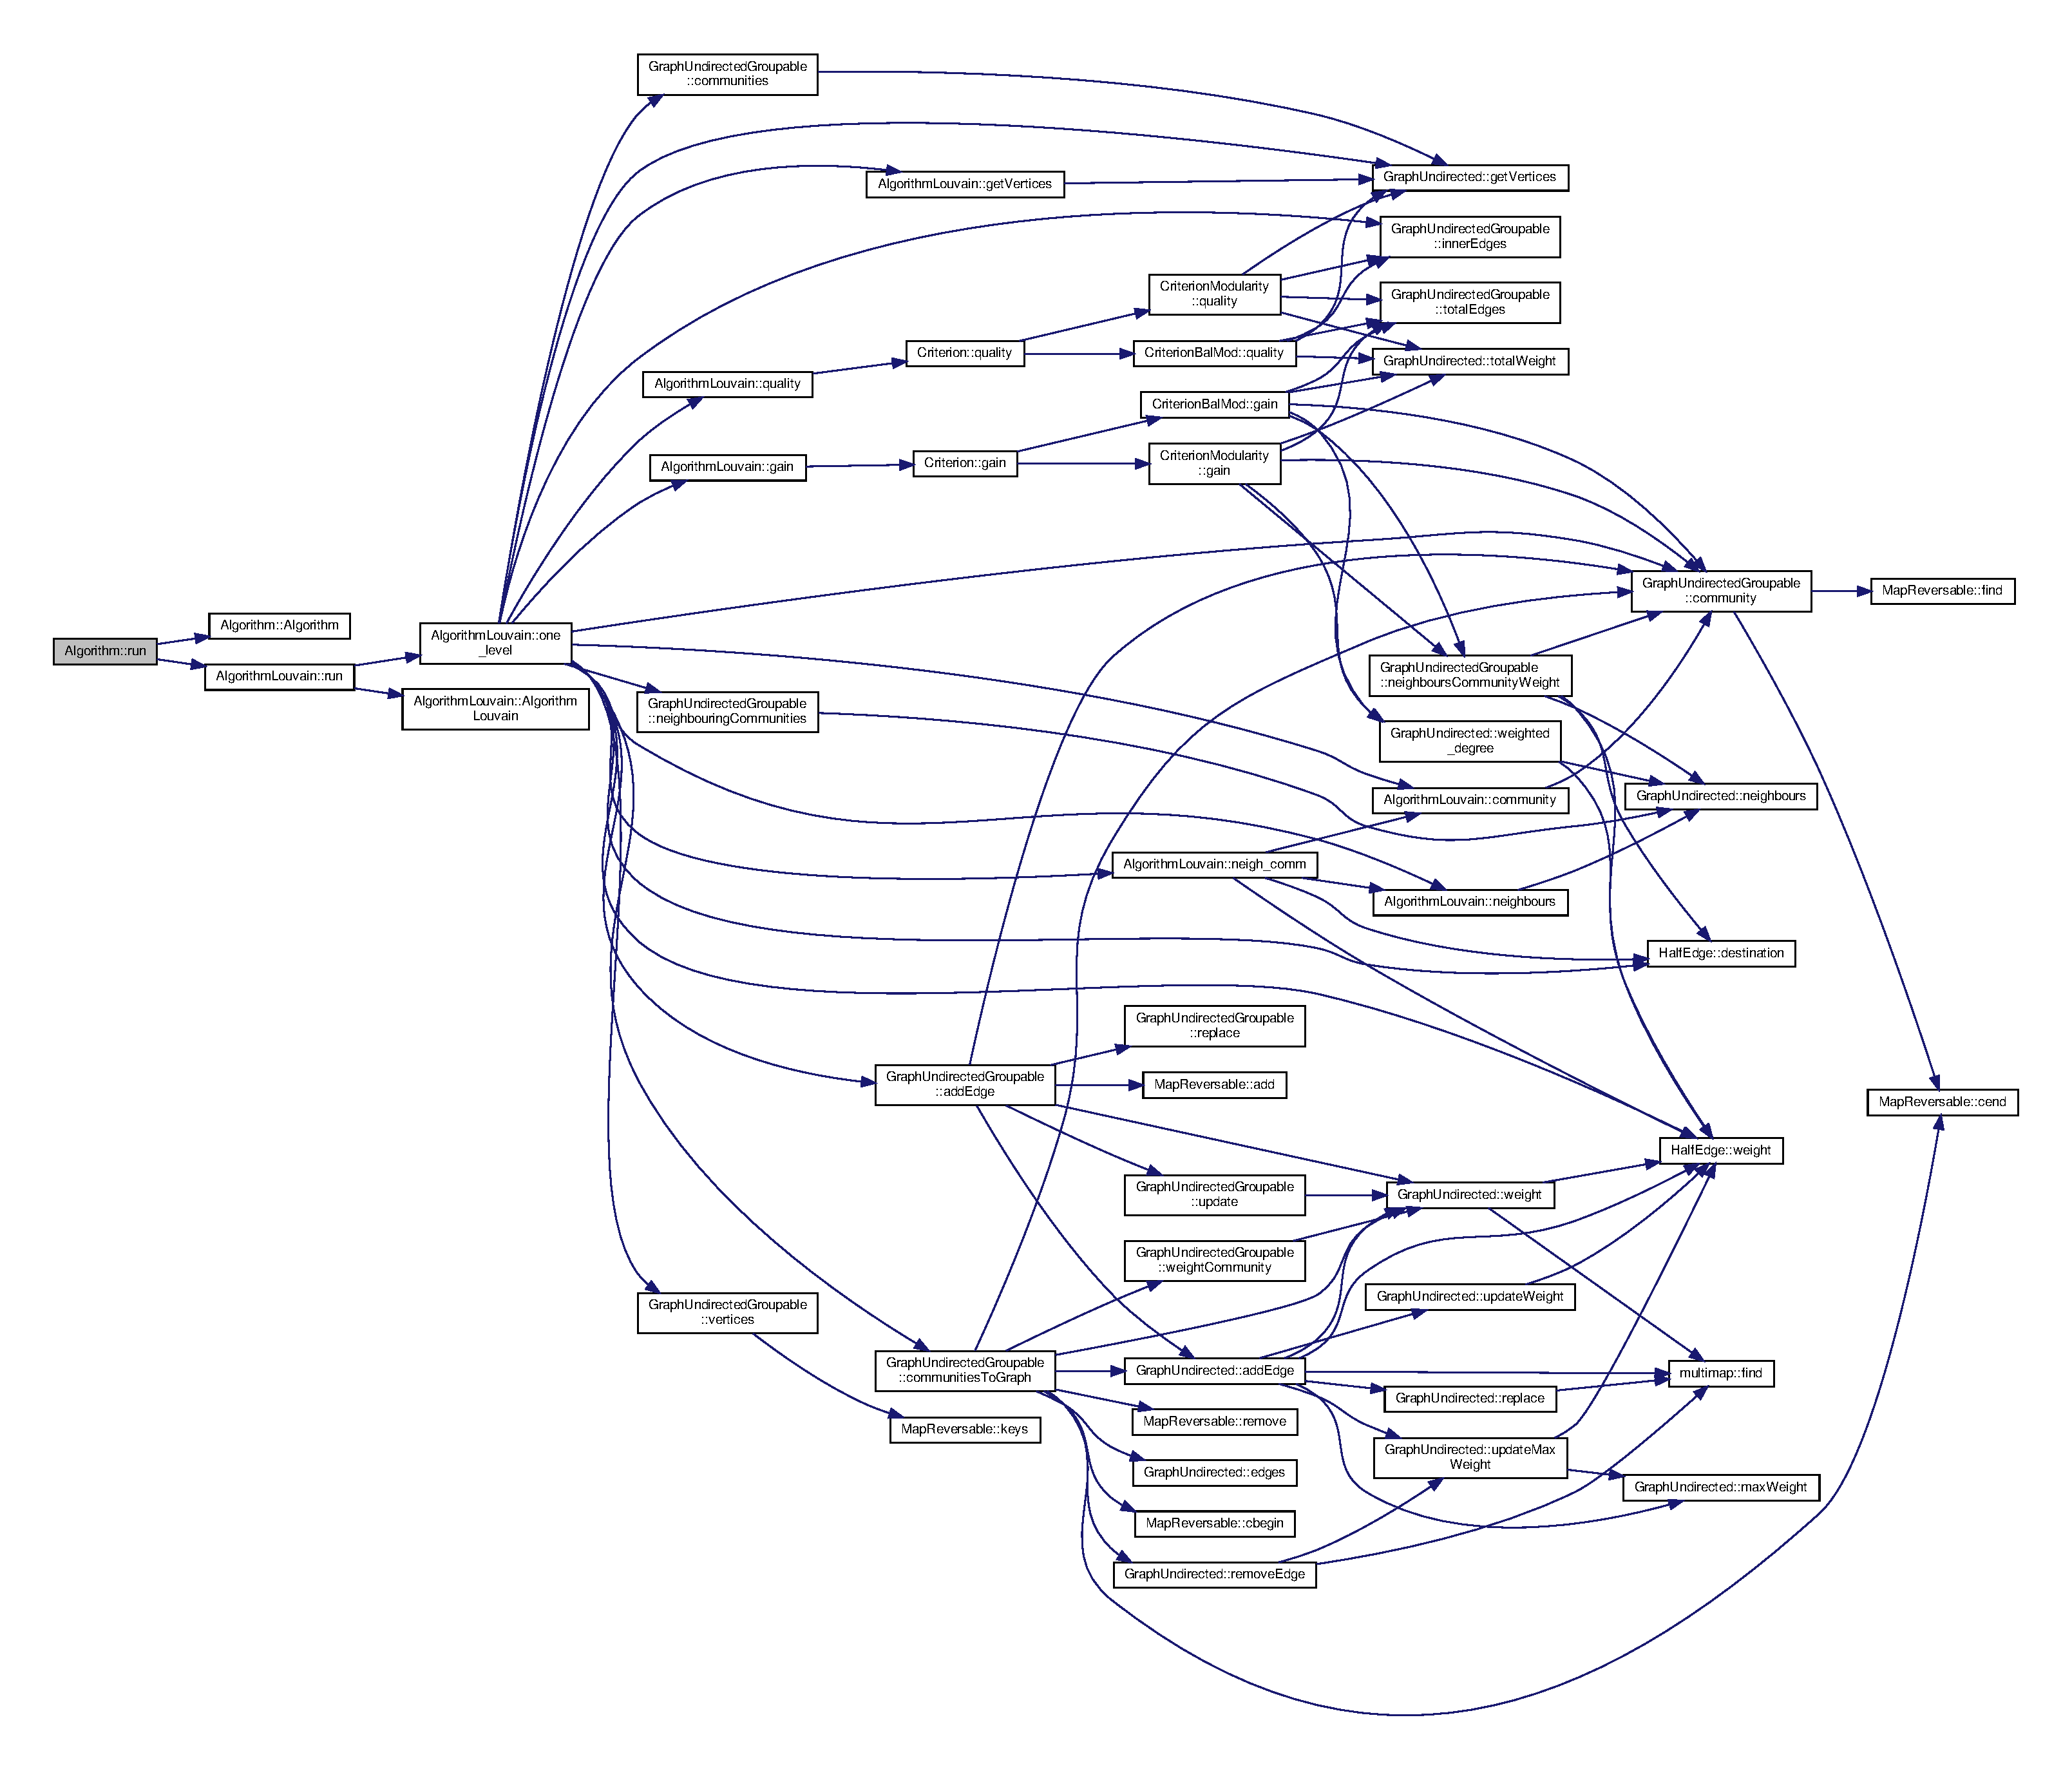
\includegraphics[width=350pt]{classAlgorithm_a10dcb6b63ba40fad0bf11a0fef7b40f5_cgraph}
\end{center}
\end{figure}
\mbox{\Hypertarget{classAlgorithm_a3b3172af613b02bfb1dc2502553d91c0}\label{classAlgorithm_a3b3172af613b02bfb1dc2502553d91c0}} 
\index{Algorithm@{Algorithm}!to\+String@{to\+String}}
\index{to\+String@{to\+String}!Algorithm@{Algorithm}}
\subsubsection{\texorpdfstring{to\+String()}{toString()}}
{\footnotesize\ttfamily const std\+::string Algorithm\+::to\+String (\begin{DoxyParamCaption}\item[{const \hyperlink{classStringFormatter}{String\+Formatter} \&}]{sf = {\ttfamily \hyperlink{stringFormatter_8h_abf1349c8e24162d0134072aff288f2a2}{default\+String\+Formatter}} }\end{DoxyParamCaption}) const\hspace{0.3cm}{\ttfamily [inline]}}

Function that converts this object to a string representation. Might be useful for debugging.


\begin{DoxyParams}{Parameters}
{\em sf} & is a String\+Formater object that facilitates formating \\
\hline
\end{DoxyParams}
\begin{DoxyReturn}{Returns}
the string representing this object 
\end{DoxyReturn}


Definition at line 254 of file algorithm.\+h.



References L\+O\+U\+V\+A\+IN, and Algorithm\+Louvain\+::to\+String().

Here is the call graph for this function\+:
\nopagebreak
\begin{figure}[H]
\begin{center}
\leavevmode
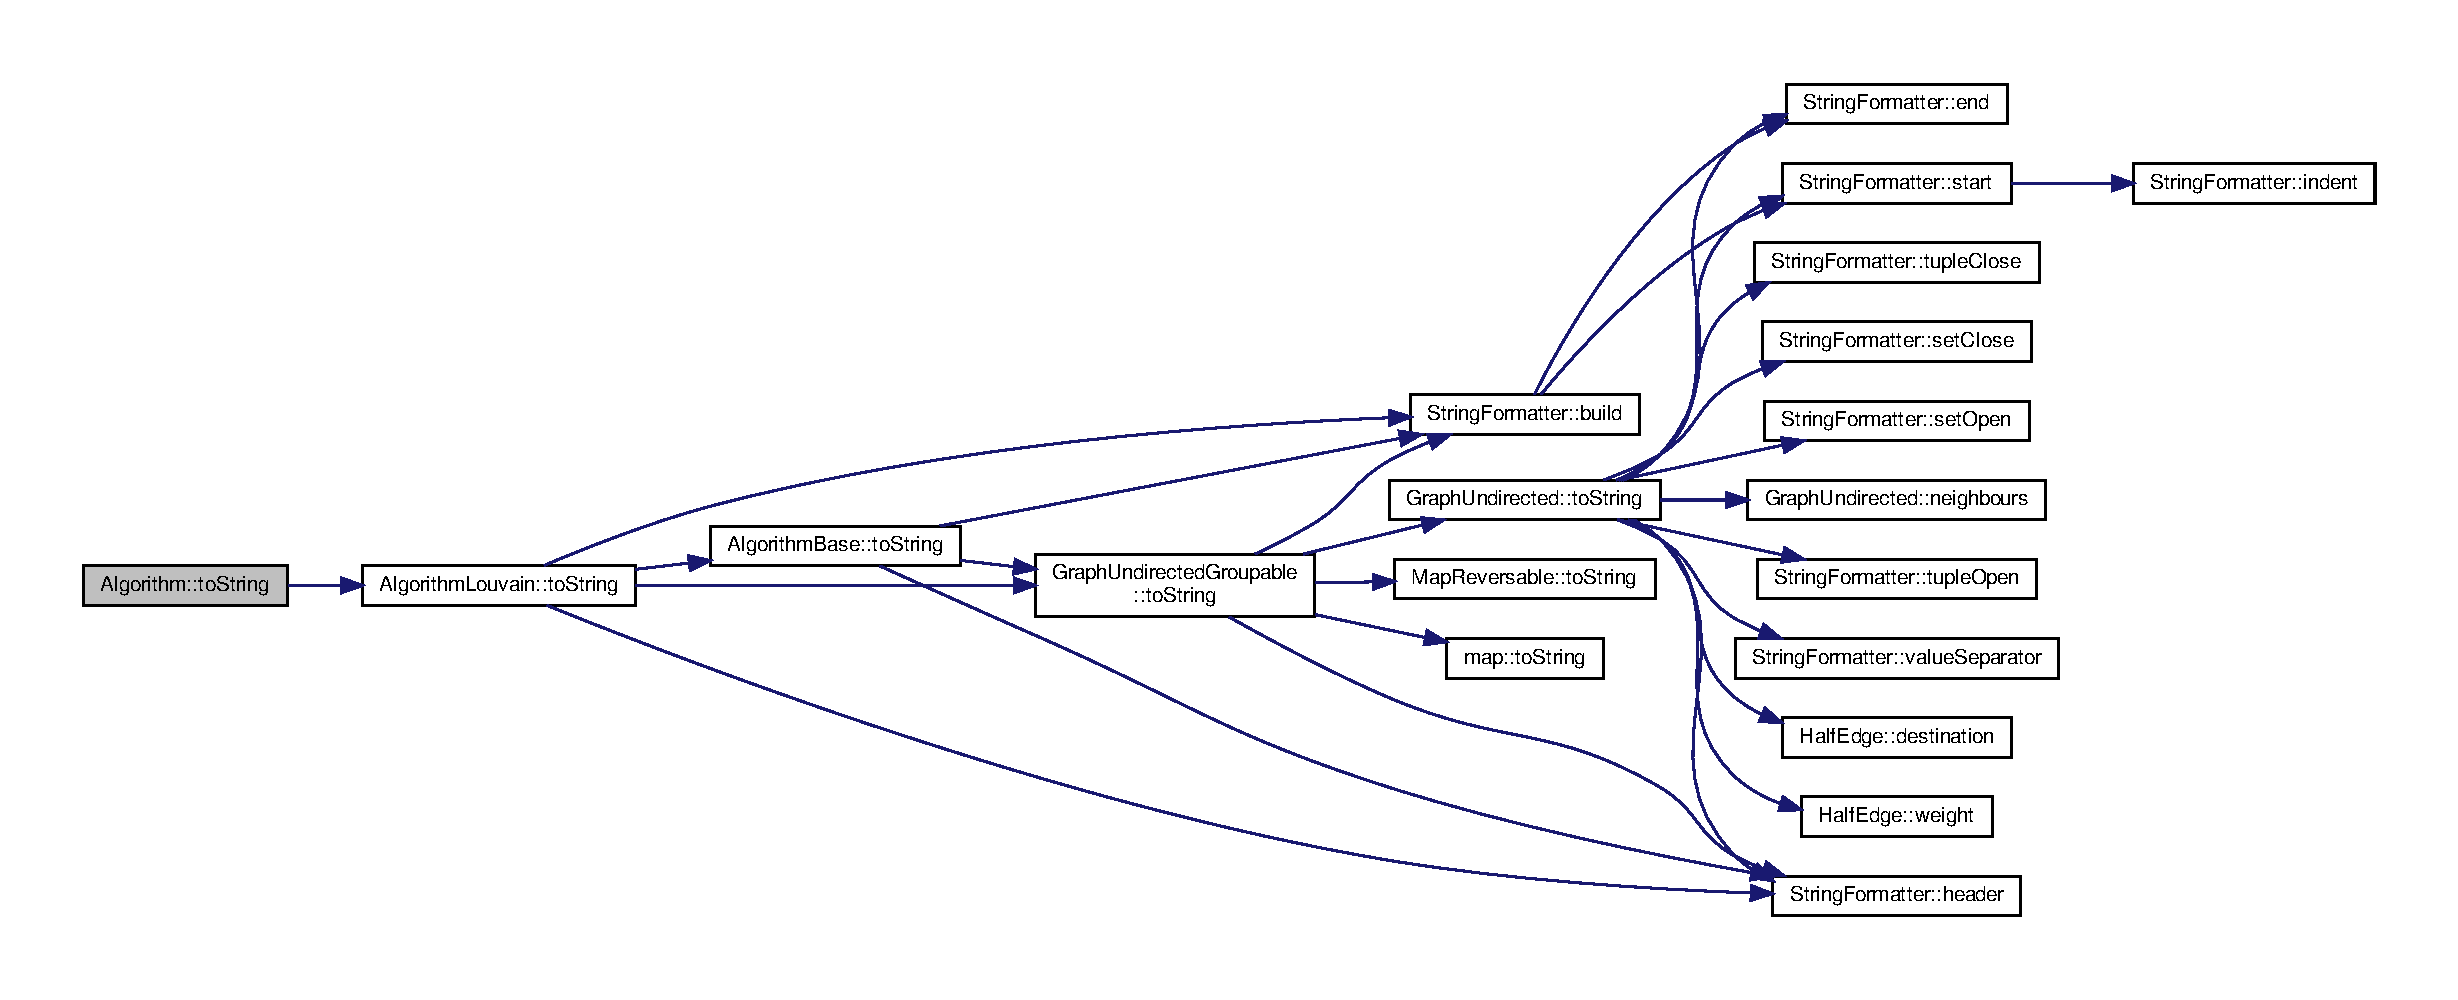
\includegraphics[width=350pt]{classAlgorithm_a3b3172af613b02bfb1dc2502553d91c0_cgraph}
\end{center}
\end{figure}


\subsection{Member Data Documentation}
\mbox{\Hypertarget{classAlgorithm_a95ef62342279e55525eacf34e83bc2ca}\label{classAlgorithm_a95ef62342279e55525eacf34e83bc2ca}} 
\index{Algorithm@{Algorithm}!algorithm\+Louvain@{algorithm\+Louvain}}
\index{algorithm\+Louvain@{algorithm\+Louvain}!Algorithm@{Algorithm}}
\subsubsection{\texorpdfstring{algorithm\+Louvain}{algorithmLouvain}}
{\footnotesize\ttfamily \hyperlink{classAlgorithmLouvain}{Algorithm\+Louvain} Algorithm\+::algorithm\+Louvain\hspace{0.3cm}{\ttfamily [private]}}



Definition at line 87 of file algorithm.\+h.

\mbox{\Hypertarget{classAlgorithm_aaee2fd7b239cc8721ec894716271dcd9}\label{classAlgorithm_aaee2fd7b239cc8721ec894716271dcd9}} 
\index{Algorithm@{Algorithm}!algrthm@{algrthm}}
\index{algrthm@{algrthm}!Algorithm@{Algorithm}}
\subsubsection{\texorpdfstring{algrthm}{algrthm}}
{\footnotesize\ttfamily const \hyperlink{classAlgorithm_a38e19a8c3dc51b97563a34d9e59a748d}{A\+L\+G\+O\+R\+I\+T\+HM} Algorithm\+::algrthm\hspace{0.3cm}{\ttfamily [private]}}



Definition at line 82 of file algorithm.\+h.



The documentation for this class was generated from the following file\+:\begin{DoxyCompactItemize}
\item 
R-\/\+C\+R\+A\+N/src/base/\+Cpp/\hyperlink{algorithm_8h}{algorithm.\+h}\end{DoxyCompactItemize}

\hypertarget{classAlgorithmBase}{}\section{Algorithm\+Base Class Reference}
\label{classAlgorithmBase}\index{Algorithm\+Base@{Algorithm\+Base}}


Base class for algorithms.  




{\ttfamily \#include $<$algorithm\+Base.\+h$>$}



Inheritance diagram for Algorithm\+Base\+:
\nopagebreak
\begin{figure}[H]
\begin{center}
\leavevmode
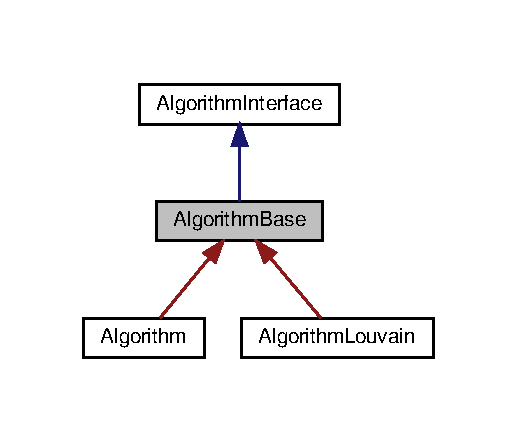
\includegraphics[width=248pt]{classAlgorithmBase__inherit__graph}
\end{center}
\end{figure}


Collaboration diagram for Algorithm\+Base\+:
\nopagebreak
\begin{figure}[H]
\begin{center}
\leavevmode
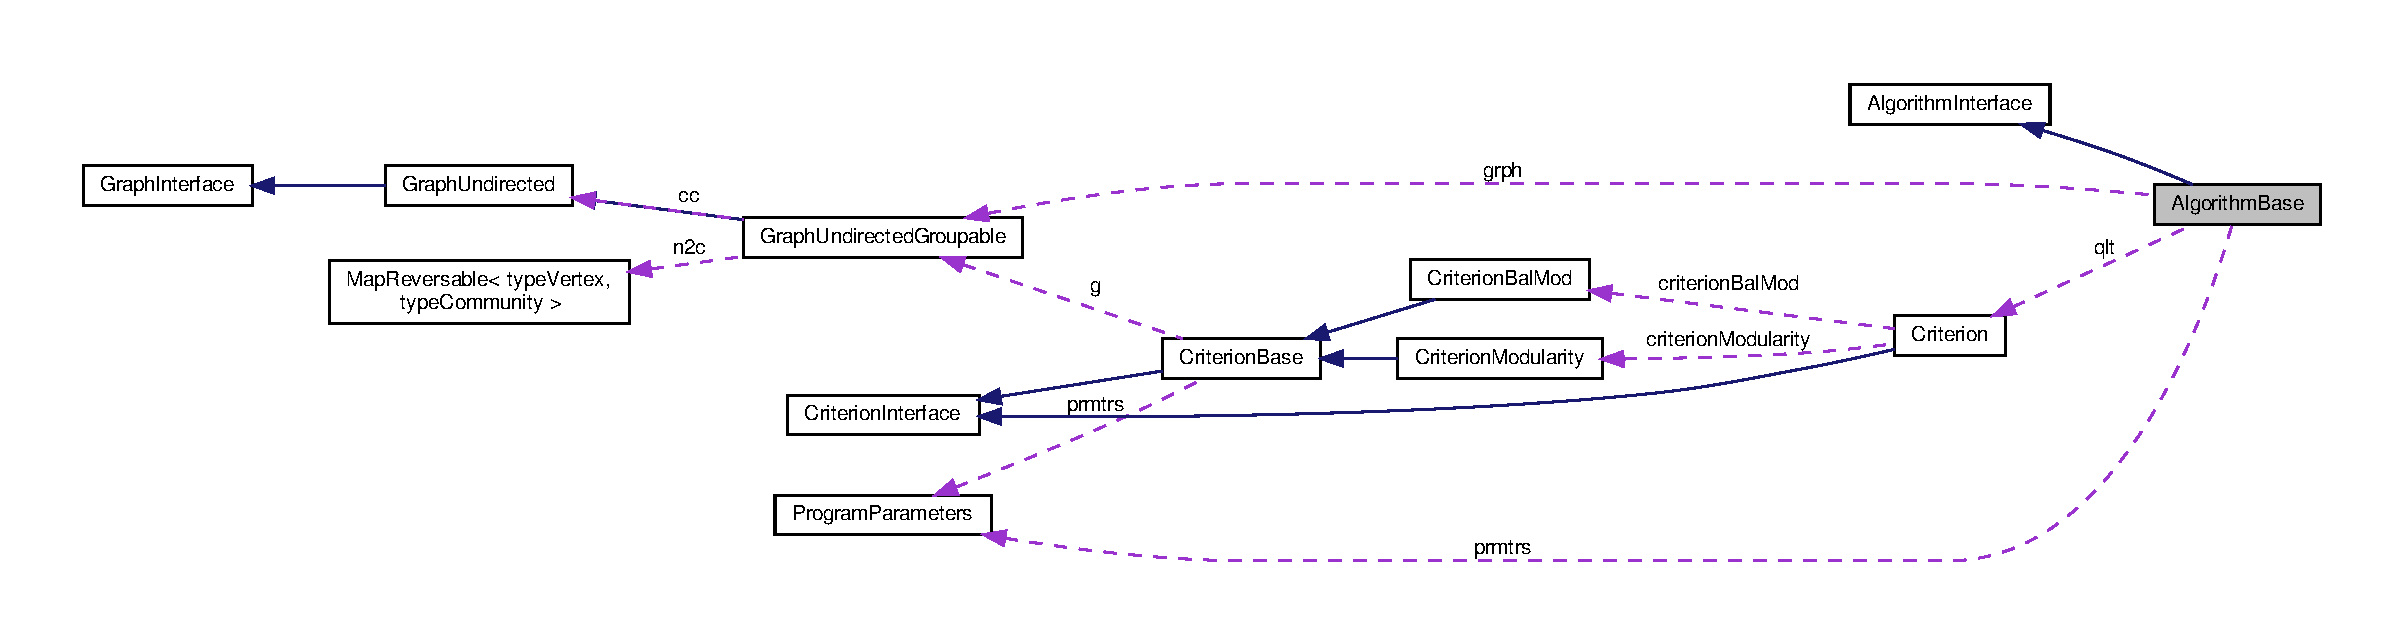
\includegraphics[width=350pt]{classAlgorithmBase__coll__graph}
\end{center}
\end{figure}
\subsection*{Public Member Functions}
\begin{DoxyCompactItemize}
\item 
\hyperlink{classAlgorithmBase_ac498e7949995484bd5a9a3188c599edf}{Algorithm\+Base} ()=delete
\item 
virtual \hyperlink{classAlgorithmBase_a01862a2fa8e29b154e6d95c1287a598e}{$\sim$\+Algorithm\+Base} ()
\item 
\hyperlink{classAlgorithmBase_aaeeeef264fa7bae05fd3663a5b8c1302}{Algorithm\+Base} (\hyperlink{classGraphUndirectedGroupable}{Graph\+Undirected\+Groupable} \&graph, const \hyperlink{classCriterion}{Criterion} \&quality, const \hyperlink{structProgramParameters}{Program\+Parameters} \&parameters=\hyperlink{program_8h_ae2d819404495f80f31db7676c1329d19}{arguments\+Default})
\item 
const std\+::string \hyperlink{classAlgorithmBase_a3041a5aebcf04f8fd8f985fd23525406}{to\+String} (const \hyperlink{classStringFormatter}{String\+Formatter} \&sf=\hyperlink{stringFormatter_8h_abf1349c8e24162d0134072aff288f2a2}{default\+String\+Formatter}) const
\end{DoxyCompactItemize}
\subsection*{Protected Attributes}
\begin{DoxyCompactItemize}
\item 
\hyperlink{classGraphUndirectedGroupable}{Graph\+Undirected\+Groupable} \& \hyperlink{classAlgorithmBase_a54b71b720b025291d9802e20874c860d}{grph}
\item 
const \hyperlink{structProgramParameters}{Program\+Parameters} \& \hyperlink{classAlgorithmBase_a69765034d365e4cab46c25ec626db528}{prmtrs}
\item 
const \hyperlink{classCriterion}{Criterion} \& \hyperlink{classAlgorithmBase_aa1e529eb903df296a7a7ef67f06537d8}{qlt}
\end{DoxyCompactItemize}
\subsection*{Additional Inherited Members}


\subsection{Detailed Description}
Base class for algorithms. 

It simply stores references to the graph, quality and program parameters objects.

This class should be extended by all algorithms. It strengths the idea that those objects should not be copied and that the quality and program parameters should not be modified.

\begin{DoxyAuthor}{Author}
poltergeist0
\end{DoxyAuthor}
\begin{DoxyDate}{Date}
2019-\/01-\/01 
\end{DoxyDate}


Definition at line 49 of file algorithm\+Base.\+h.



\subsection{Constructor \& Destructor Documentation}
\mbox{\Hypertarget{classAlgorithmBase_ac498e7949995484bd5a9a3188c599edf}\label{classAlgorithmBase_ac498e7949995484bd5a9a3188c599edf}} 
\index{Algorithm\+Base@{Algorithm\+Base}!Algorithm\+Base@{Algorithm\+Base}}
\index{Algorithm\+Base@{Algorithm\+Base}!Algorithm\+Base@{Algorithm\+Base}}
\subsubsection{\texorpdfstring{Algorithm\+Base()}{AlgorithmBase()}\hspace{0.1cm}{\footnotesize\ttfamily [1/2]}}
{\footnotesize\ttfamily Algorithm\+Base\+::\+Algorithm\+Base (\begin{DoxyParamCaption}{ }\end{DoxyParamCaption})\hspace{0.3cm}{\ttfamily [delete]}}

Default constructor not acceptable. Must be passed at least the graph, quality and parameters. \mbox{\Hypertarget{classAlgorithmBase_a01862a2fa8e29b154e6d95c1287a598e}\label{classAlgorithmBase_a01862a2fa8e29b154e6d95c1287a598e}} 
\index{Algorithm\+Base@{Algorithm\+Base}!````~Algorithm\+Base@{$\sim$\+Algorithm\+Base}}
\index{````~Algorithm\+Base@{$\sim$\+Algorithm\+Base}!Algorithm\+Base@{Algorithm\+Base}}
\subsubsection{\texorpdfstring{$\sim$\+Algorithm\+Base()}{~AlgorithmBase()}}
{\footnotesize\ttfamily virtual Algorithm\+Base\+::$\sim$\+Algorithm\+Base (\begin{DoxyParamCaption}{ }\end{DoxyParamCaption})\hspace{0.3cm}{\ttfamily [inline]}, {\ttfamily [virtual]}}

Destructor 

Definition at line 65 of file algorithm\+Base.\+h.

\mbox{\Hypertarget{classAlgorithmBase_aaeeeef264fa7bae05fd3663a5b8c1302}\label{classAlgorithmBase_aaeeeef264fa7bae05fd3663a5b8c1302}} 
\index{Algorithm\+Base@{Algorithm\+Base}!Algorithm\+Base@{Algorithm\+Base}}
\index{Algorithm\+Base@{Algorithm\+Base}!Algorithm\+Base@{Algorithm\+Base}}
\subsubsection{\texorpdfstring{Algorithm\+Base()}{AlgorithmBase()}\hspace{0.1cm}{\footnotesize\ttfamily [2/2]}}
{\footnotesize\ttfamily Algorithm\+Base\+::\+Algorithm\+Base (\begin{DoxyParamCaption}\item[{\hyperlink{classGraphUndirectedGroupable}{Graph\+Undirected\+Groupable} \&}]{graph,  }\item[{const \hyperlink{classCriterion}{Criterion} \&}]{quality,  }\item[{const \hyperlink{structProgramParameters}{Program\+Parameters} \&}]{parameters = {\ttfamily \hyperlink{program_8h_ae2d819404495f80f31db7676c1329d19}{arguments\+Default}} }\end{DoxyParamCaption})\hspace{0.3cm}{\ttfamily [inline]}}

Constructor.


\begin{DoxyParams}{Parameters}
{\em graph} & reference to the graph object \\
\hline
{\em quality} & reference to the quality object \\
\hline
{\em parameters} & reference to the parameters object \\
\hline
\end{DoxyParams}


Definition at line 74 of file algorithm\+Base.\+h.



\subsection{Member Function Documentation}
\mbox{\Hypertarget{classAlgorithmBase_a3041a5aebcf04f8fd8f985fd23525406}\label{classAlgorithmBase_a3041a5aebcf04f8fd8f985fd23525406}} 
\index{Algorithm\+Base@{Algorithm\+Base}!to\+String@{to\+String}}
\index{to\+String@{to\+String}!Algorithm\+Base@{Algorithm\+Base}}
\subsubsection{\texorpdfstring{to\+String()}{toString()}}
{\footnotesize\ttfamily const std\+::string Algorithm\+Base\+::to\+String (\begin{DoxyParamCaption}\item[{const \hyperlink{classStringFormatter}{String\+Formatter} \&}]{sf = {\ttfamily \hyperlink{stringFormatter_8h_abf1349c8e24162d0134072aff288f2a2}{default\+String\+Formatter}} }\end{DoxyParamCaption}) const\hspace{0.3cm}{\ttfamily [inline]}}

Function that converts this object to a string representation. Might be useful for debugging.


\begin{DoxyParams}{Parameters}
{\em sf} & is a String\+Formater object that facilitates formating \\
\hline
\end{DoxyParams}
\begin{DoxyReturn}{Returns}
the string representing this object 
\end{DoxyReturn}


Definition at line 92 of file algorithm\+Base.\+h.



References String\+Formatter\+::build(), String\+Formatter\+::header(), and Graph\+Undirected\+Groupable\+::to\+String().



Referenced by Algorithm\+Louvain\+::to\+String().

Here is the call graph for this function\+:
\nopagebreak
\begin{figure}[H]
\begin{center}
\leavevmode
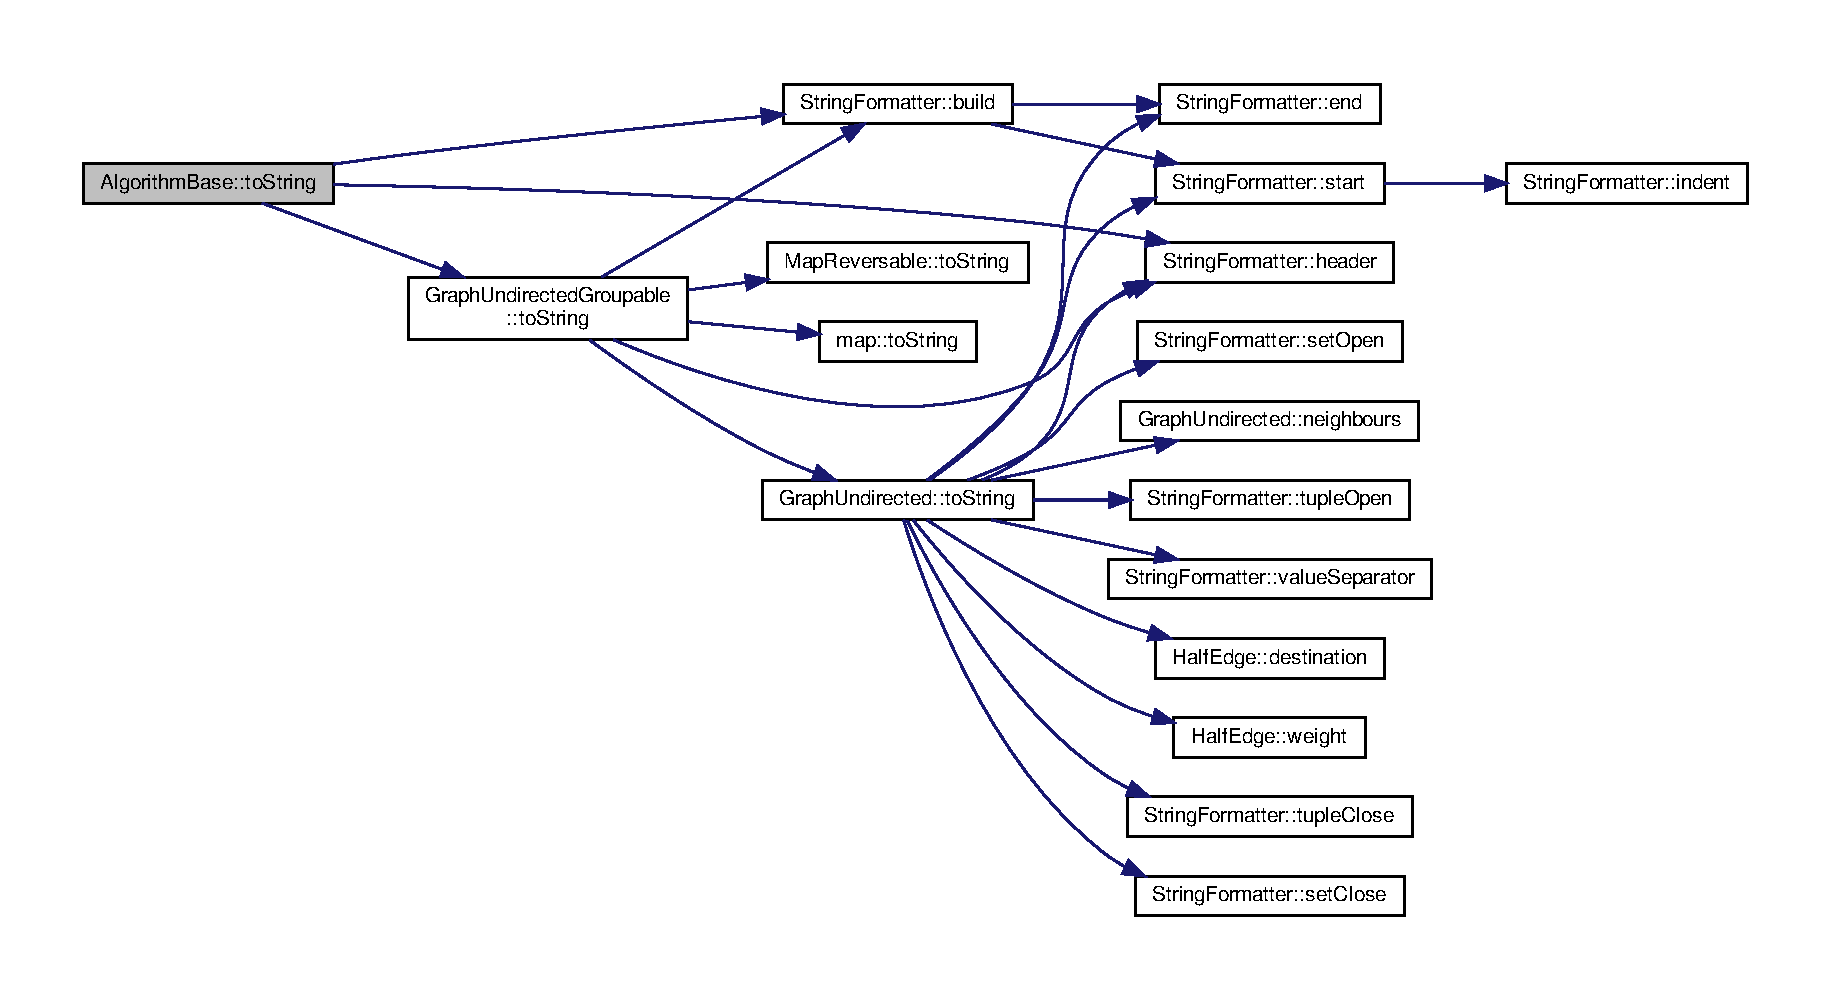
\includegraphics[width=350pt]{classAlgorithmBase_a3041a5aebcf04f8fd8f985fd23525406_cgraph}
\end{center}
\end{figure}


\subsection{Member Data Documentation}
\mbox{\Hypertarget{classAlgorithmBase_a54b71b720b025291d9802e20874c860d}\label{classAlgorithmBase_a54b71b720b025291d9802e20874c860d}} 
\index{Algorithm\+Base@{Algorithm\+Base}!grph@{grph}}
\index{grph@{grph}!Algorithm\+Base@{Algorithm\+Base}}
\subsubsection{\texorpdfstring{grph}{grph}}
{\footnotesize\ttfamily \hyperlink{classGraphUndirectedGroupable}{Graph\+Undirected\+Groupable}\& Algorithm\+Base\+::grph\hspace{0.3cm}{\ttfamily [protected]}}



Definition at line 51 of file algorithm\+Base.\+h.



Referenced by Algorithm\+Louvain\+::add\+Remove\+Edge\+Post(), Algorithm\+Louvain\+::add\+Remove\+Edge\+Pre(), Algorithm\+::add\+Remove\+Edges(), Algorithm\+Louvain\+::community(), Algorithm\+Louvain\+::community\+Count(), Algorithm\+Louvain\+::disband(), Algorithm\+Louvain\+::edge\+Count(), Algorithm\+Louvain\+::edges(), Algorithm\+Louvain\+::get\+Vertices(), Algorithm\+Louvain\+::inner\+Edges(), Algorithm\+Louvain\+::max\+Weight(), Algorithm\+Louvain\+::neighbors(), Algorithm\+Louvain\+::neighbors\+Community\+Count(), Algorithm\+Louvain\+::neighbors\+Community\+Weight(), Algorithm\+Louvain\+::neighbors\+Count(), Algorithm\+Louvain\+::one\+\_\+level(), Algorithm\+Louvain\+::total\+Edges(), Algorithm\+Louvain\+::total\+Weight(), Algorithm\+Louvain\+::vertices(), Algorithm\+Louvain\+::vertices\+Count(), and Algorithm\+Louvain\+::weighted\+\_\+degree().

\mbox{\Hypertarget{classAlgorithmBase_a69765034d365e4cab46c25ec626db528}\label{classAlgorithmBase_a69765034d365e4cab46c25ec626db528}} 
\index{Algorithm\+Base@{Algorithm\+Base}!prmtrs@{prmtrs}}
\index{prmtrs@{prmtrs}!Algorithm\+Base@{Algorithm\+Base}}
\subsubsection{\texorpdfstring{prmtrs}{prmtrs}}
{\footnotesize\ttfamily const \hyperlink{structProgramParameters}{Program\+Parameters}\& Algorithm\+Base\+::prmtrs\hspace{0.3cm}{\ttfamily [protected]}}



Definition at line 52 of file algorithm\+Base.\+h.



Referenced by Algorithm\+Louvain\+::one\+\_\+level().

\mbox{\Hypertarget{classAlgorithmBase_aa1e529eb903df296a7a7ef67f06537d8}\label{classAlgorithmBase_aa1e529eb903df296a7a7ef67f06537d8}} 
\index{Algorithm\+Base@{Algorithm\+Base}!qlt@{qlt}}
\index{qlt@{qlt}!Algorithm\+Base@{Algorithm\+Base}}
\subsubsection{\texorpdfstring{qlt}{qlt}}
{\footnotesize\ttfamily const \hyperlink{classCriterion}{Criterion}\& Algorithm\+Base\+::qlt\hspace{0.3cm}{\ttfamily [protected]}}



Definition at line 53 of file algorithm\+Base.\+h.



Referenced by Algorithm\+Louvain\+::gain(), and Algorithm\+Louvain\+::quality().



The documentation for this class was generated from the following file\+:\begin{DoxyCompactItemize}
\item 
R-\/\+C\+R\+A\+N/src/base/\+Cpp/\hyperlink{algorithmBase_8h}{algorithm\+Base.\+h}\end{DoxyCompactItemize}

\hypertarget{classAlgorithmInterface}{}\section{Algorithm\+Interface Class Reference}
\label{classAlgorithmInterface}\index{Algorithm\+Interface@{Algorithm\+Interface}}


Algorithms A\+PI.  




{\ttfamily \#include $<$algorithm\+Interface.\+h$>$}



Inheritance diagram for Algorithm\+Interface\+:
\nopagebreak
\begin{figure}[H]
\begin{center}
\leavevmode
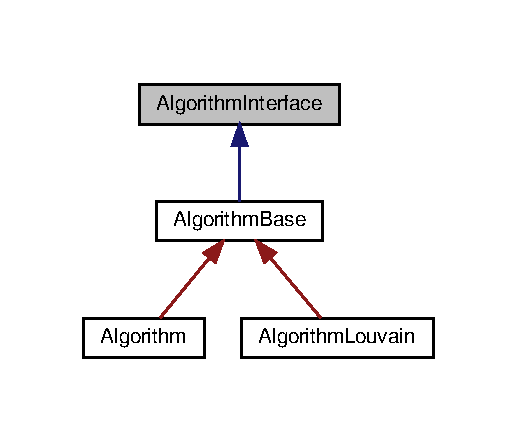
\includegraphics[width=248pt]{classAlgorithmInterface__inherit__graph}
\end{center}
\end{figure}
\subsection*{Public Member Functions}
\begin{DoxyCompactItemize}
\item 
virtual \hyperlink{classAlgorithmInterface_a240e65a4c0c5bdca207abf39733fe3fc}{$\sim$\+Algorithm\+Interface} ()
\end{DoxyCompactItemize}
\subsection*{Protected Member Functions}
\begin{DoxyCompactItemize}
\item 
virtual bool \hyperlink{classAlgorithmInterface_ae5a6e84b139768dff92a70cacaec7472}{add\+Remove\+Edge\+Pre} (const \hyperlink{edge_8h_a5fbd20c46956d479cb10afc9855223f6}{type\+Vertex} \&source, const \hyperlink{edge_8h_a5fbd20c46956d479cb10afc9855223f6}{type\+Vertex} \&destination, const \hyperlink{edge_8h_a2e7ea3be891ac8b52f749ec73fee6dd2}{type\+Weight} \&weight=1.\+0)=0
\item 
virtual bool \hyperlink{classAlgorithmInterface_ac97ed4df4fd2b14b16d55c1b3b9749b6}{add\+Remove\+Edge\+Post} (const \hyperlink{edge_8h_a5fbd20c46956d479cb10afc9855223f6}{type\+Vertex} \&source, const \hyperlink{edge_8h_a5fbd20c46956d479cb10afc9855223f6}{type\+Vertex} \&destination, const \hyperlink{edge_8h_a2e7ea3be891ac8b52f749ec73fee6dd2}{type\+Weight} \&weight=1.\+0)=0
\item 
virtual bool \hyperlink{classAlgorithmInterface_a0bafcdabd2b5fd45abe97af91e02ca14}{run} ()=0
\end{DoxyCompactItemize}


\subsection{Detailed Description}
Algorithms A\+PI. 

All algorithms must implement the functions defined in this class.

Also, at the end of this class, there are two comments with the skeletons of two constructors that must be defined in classes that implement this interface.

The first is the deletion of the default constructor which should not exist. Calling a constructor without the graph, quality and program parameters is not permitted.

The second constructor is the one that must be called and that receives the graph, quality and program parameters.

\begin{DoxyAuthor}{Author}
poltergeist0
\end{DoxyAuthor}
\begin{DoxyDate}{Date}
2019-\/01-\/01 
\end{DoxyDate}


Definition at line 76 of file algorithm\+Interface.\+h.



\subsection{Constructor \& Destructor Documentation}
\mbox{\Hypertarget{classAlgorithmInterface_a240e65a4c0c5bdca207abf39733fe3fc}\label{classAlgorithmInterface_a240e65a4c0c5bdca207abf39733fe3fc}} 
\index{Algorithm\+Interface@{Algorithm\+Interface}!````~Algorithm\+Interface@{$\sim$\+Algorithm\+Interface}}
\index{````~Algorithm\+Interface@{$\sim$\+Algorithm\+Interface}!Algorithm\+Interface@{Algorithm\+Interface}}
\subsubsection{\texorpdfstring{$\sim$\+Algorithm\+Interface()}{~AlgorithmInterface()}}
{\footnotesize\ttfamily virtual Algorithm\+Interface\+::$\sim$\+Algorithm\+Interface (\begin{DoxyParamCaption}{ }\end{DoxyParamCaption})\hspace{0.3cm}{\ttfamily [inline]}, {\ttfamily [virtual]}}

Destructor 

Definition at line 117 of file algorithm\+Interface.\+h.



\subsection{Member Function Documentation}
\mbox{\Hypertarget{classAlgorithmInterface_ac97ed4df4fd2b14b16d55c1b3b9749b6}\label{classAlgorithmInterface_ac97ed4df4fd2b14b16d55c1b3b9749b6}} 
\index{Algorithm\+Interface@{Algorithm\+Interface}!add\+Remove\+Edge\+Post@{add\+Remove\+Edge\+Post}}
\index{add\+Remove\+Edge\+Post@{add\+Remove\+Edge\+Post}!Algorithm\+Interface@{Algorithm\+Interface}}
\subsubsection{\texorpdfstring{add\+Remove\+Edge\+Post()}{addRemoveEdgePost()}}
{\footnotesize\ttfamily virtual bool Algorithm\+Interface\+::add\+Remove\+Edge\+Post (\begin{DoxyParamCaption}\item[{const \hyperlink{edge_8h_a5fbd20c46956d479cb10afc9855223f6}{type\+Vertex} \&}]{source,  }\item[{const \hyperlink{edge_8h_a5fbd20c46956d479cb10afc9855223f6}{type\+Vertex} \&}]{destination,  }\item[{const \hyperlink{edge_8h_a2e7ea3be891ac8b52f749ec73fee6dd2}{type\+Weight} \&}]{weight = {\ttfamily 1.0} }\end{DoxyParamCaption})\hspace{0.3cm}{\ttfamily [protected]}, {\ttfamily [pure virtual]}}

Function execute after adding or removing a single edge from the graph. It is used internally by the add\+Remove\+Edges function of class \char`\"{}\+Algorithm\char`\"{}. Useful if post-\/processing is required, for example, to update some of variables after the edge has be added or removed. Any edge with a weight different from zero is inserted. Any edge with a weight of exactly zero is removed. 
\begin{DoxyParams}{Parameters}
{\em source} & source vertex \\
\hline
{\em destination} & destination vertex \\
\hline
{\em weight} & optional if adding an edge. Must be exactly zero to remove an edge. \\
\hline
\end{DoxyParams}
\begin{DoxyReturn}{Returns}
true if all operations succeeded. False, otherwise. 
\end{DoxyReturn}


Implemented in \hyperlink{classAlgorithmLouvain_a69f296749859441c8a3844753bdd58e5}{Algorithm\+Louvain}, and \hyperlink{classAlgorithm_ad78e2c5819da723c373ce6d4a28ac36d}{Algorithm}.

\mbox{\Hypertarget{classAlgorithmInterface_ae5a6e84b139768dff92a70cacaec7472}\label{classAlgorithmInterface_ae5a6e84b139768dff92a70cacaec7472}} 
\index{Algorithm\+Interface@{Algorithm\+Interface}!add\+Remove\+Edge\+Pre@{add\+Remove\+Edge\+Pre}}
\index{add\+Remove\+Edge\+Pre@{add\+Remove\+Edge\+Pre}!Algorithm\+Interface@{Algorithm\+Interface}}
\subsubsection{\texorpdfstring{add\+Remove\+Edge\+Pre()}{addRemoveEdgePre()}}
{\footnotesize\ttfamily virtual bool Algorithm\+Interface\+::add\+Remove\+Edge\+Pre (\begin{DoxyParamCaption}\item[{const \hyperlink{edge_8h_a5fbd20c46956d479cb10afc9855223f6}{type\+Vertex} \&}]{source,  }\item[{const \hyperlink{edge_8h_a5fbd20c46956d479cb10afc9855223f6}{type\+Vertex} \&}]{destination,  }\item[{const \hyperlink{edge_8h_a2e7ea3be891ac8b52f749ec73fee6dd2}{type\+Weight} \&}]{weight = {\ttfamily 1.0} }\end{DoxyParamCaption})\hspace{0.3cm}{\ttfamily [protected]}, {\ttfamily [pure virtual]}}

Function to execute before adding or removing a single edge from the graph. It is used internally by the add\+Remove\+Edges function of class \char`\"{}\+Algorithm\char`\"{}. Useful if pre-\/processing is required, for example, to update some of variables before the edge can be added or removed. Any edge with a weight different from zero is inserted. Any edge with a weight of exactly zero is removed. 
\begin{DoxyParams}{Parameters}
{\em source} & source vertex \\
\hline
{\em destination} & destination vertex \\
\hline
{\em weight} & optional if adding an edge. Must be exactly zero to remove an edge. \\
\hline
\end{DoxyParams}
\begin{DoxyReturn}{Returns}
true if all operations succeeded. False, otherwise. 
\end{DoxyReturn}


Implemented in \hyperlink{classAlgorithmLouvain_a883c922bf2f3c3aadb9db4962c0d8dce}{Algorithm\+Louvain}, and \hyperlink{classAlgorithm_a5835b23797b9d00f4090b996660af5d4}{Algorithm}.

\mbox{\Hypertarget{classAlgorithmInterface_a0bafcdabd2b5fd45abe97af91e02ca14}\label{classAlgorithmInterface_a0bafcdabd2b5fd45abe97af91e02ca14}} 
\index{Algorithm\+Interface@{Algorithm\+Interface}!run@{run}}
\index{run@{run}!Algorithm\+Interface@{Algorithm\+Interface}}
\subsubsection{\texorpdfstring{run()}{run()}}
{\footnotesize\ttfamily virtual bool Algorithm\+Interface\+::run (\begin{DoxyParamCaption}{ }\end{DoxyParamCaption})\hspace{0.3cm}{\ttfamily [protected]}, {\ttfamily [pure virtual]}}

Function where the actual algorithm is implemented It is called at the end of the add\+Remove\+Edges function of class \char`\"{}\+Algorithm\char`\"{}. \begin{DoxyReturn}{Returns}
true if all operations succeeded. False, otherwise. 
\end{DoxyReturn}


Implemented in \hyperlink{classAlgorithmLouvain_a0a72b9dda25c69d19996dc7448924c13}{Algorithm\+Louvain}, and \hyperlink{classAlgorithm_a10dcb6b63ba40fad0bf11a0fef7b40f5}{Algorithm}.



The documentation for this class was generated from the following file\+:\begin{DoxyCompactItemize}
\item 
R-\/\+C\+R\+A\+N/src/base/\+Cpp/\hyperlink{algorithmInterface_8h}{algorithm\+Interface.\+h}\end{DoxyCompactItemize}

\hypertarget{classAlgorithmLouvain}{}\section{Algorithm\+Louvain Class Reference}
\label{classAlgorithmLouvain}\index{Algorithm\+Louvain@{Algorithm\+Louvain}}


Class that implements the Dynamic Louvain algorithm.  




{\ttfamily \#include $<$algorithm\+Louvain.\+h$>$}



Inheritance diagram for Algorithm\+Louvain\+:
\nopagebreak
\begin{figure}[H]
\begin{center}
\leavevmode
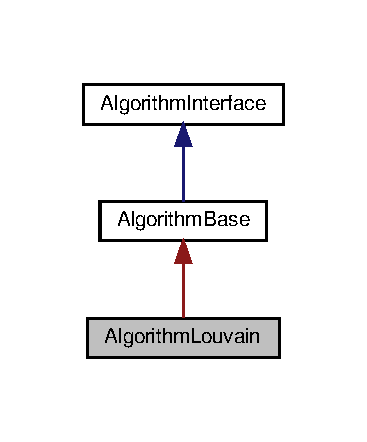
\includegraphics[width=176pt]{classAlgorithmLouvain__inherit__graph}
\end{center}
\end{figure}


Collaboration diagram for Algorithm\+Louvain\+:
\nopagebreak
\begin{figure}[H]
\begin{center}
\leavevmode
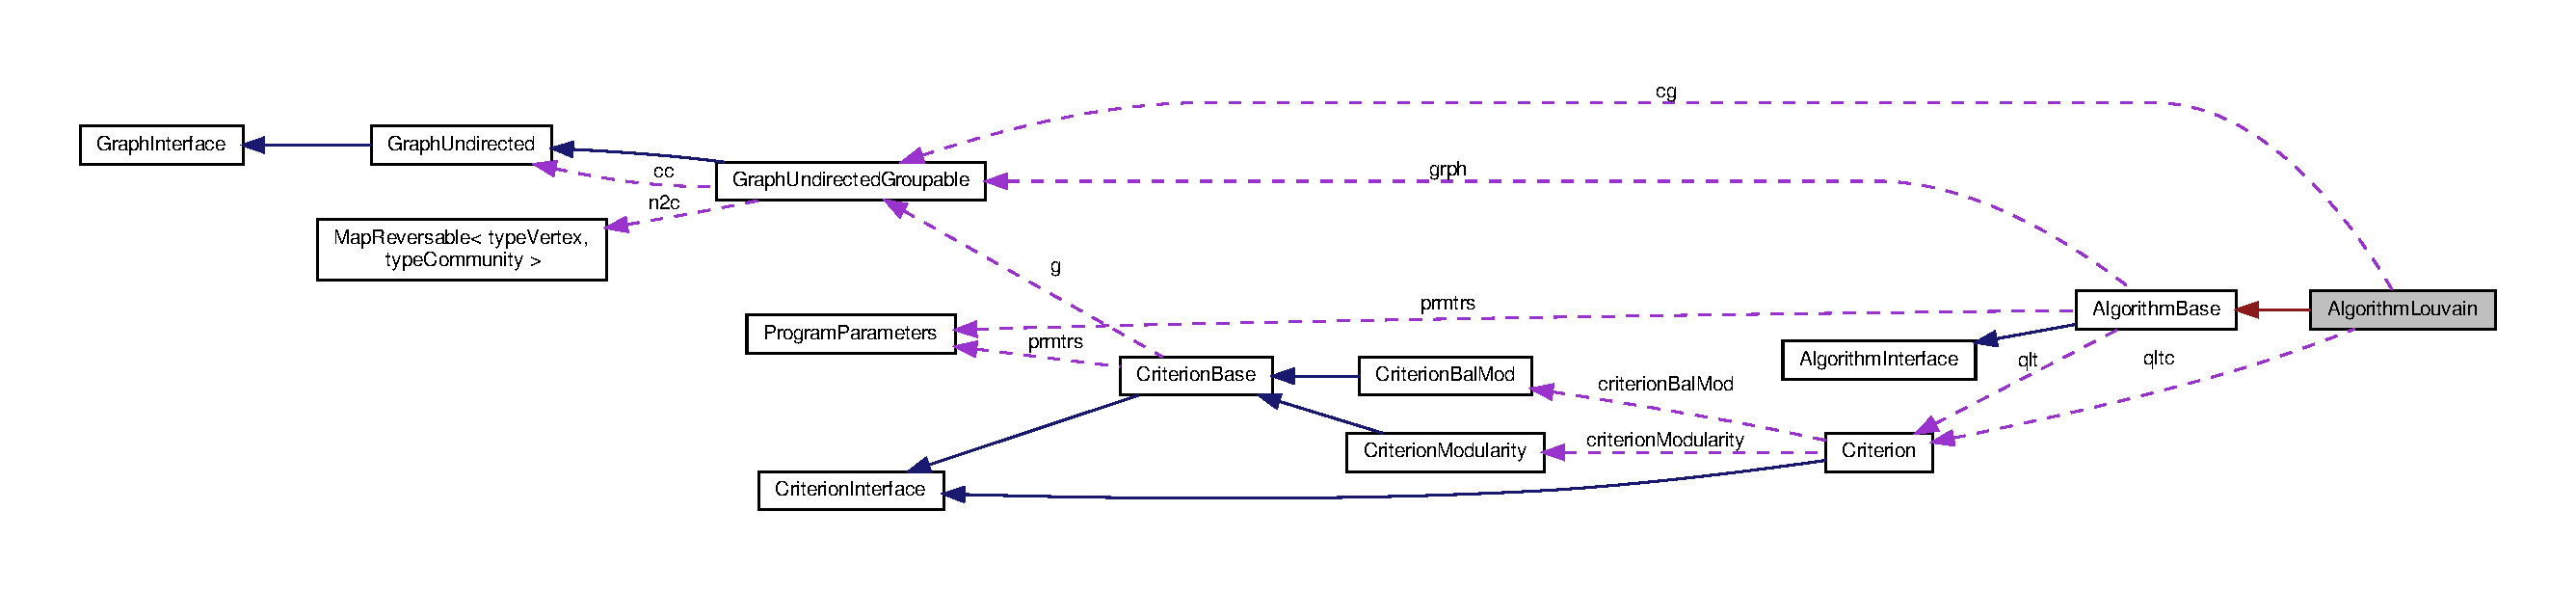
\includegraphics[width=350pt]{classAlgorithmLouvain__coll__graph}
\end{center}
\end{figure}
\subsection*{Public Member Functions}
\begin{DoxyCompactItemize}
\item 
bool \hyperlink{classAlgorithmLouvain_a883c922bf2f3c3aadb9db4962c0d8dce}{add\+Remove\+Edge\+Pre} (const \hyperlink{edge_8h_a5fbd20c46956d479cb10afc9855223f6}{type\+Vertex} \&source, const \hyperlink{edge_8h_a5fbd20c46956d479cb10afc9855223f6}{type\+Vertex} \&destination, const \hyperlink{edge_8h_a2e7ea3be891ac8b52f749ec73fee6dd2}{type\+Weight} \&weight=1.\+0)
\item 
bool \hyperlink{classAlgorithmLouvain_a69f296749859441c8a3844753bdd58e5}{add\+Remove\+Edge\+Post} (const \hyperlink{edge_8h_a5fbd20c46956d479cb10afc9855223f6}{type\+Vertex} \&source, const \hyperlink{edge_8h_a5fbd20c46956d479cb10afc9855223f6}{type\+Vertex} \&destination, const \hyperlink{edge_8h_a2e7ea3be891ac8b52f749ec73fee6dd2}{type\+Weight} \&weight=1.\+0)
\item 
bool \hyperlink{classAlgorithmLouvain_a0a72b9dda25c69d19996dc7448924c13}{run} ()
\item 
\hyperlink{classAlgorithmLouvain_ada8cb9a0c018ca6d5162b1b533ad400c}{Algorithm\+Louvain} ()=delete
\item 
\hyperlink{classAlgorithmLouvain_af39d19eff13dc68f4f5ef3a113c361e1}{$\sim$\+Algorithm\+Louvain} ()
\item 
\hyperlink{classAlgorithmLouvain_a44cd235ecff85b3896fe5d30e0b5da9a}{Algorithm\+Louvain} (\hyperlink{classGraphUndirectedGroupable}{Graph\+Undirected\+Groupable} \&graph, const \hyperlink{classCriterion}{Criterion} \&\hyperlink{classAlgorithmLouvain_a8c9b7694fff17eb5d8044cd26d7914e7}{quality}, const \hyperlink{structProgramParameters}{Program\+Parameters} \&algorithm\+Parameters=\hyperlink{program_8h_ae2d819404495f80f31db7676c1329d19}{arguments\+Default})
\item 
const std\+::string \hyperlink{classAlgorithmLouvain_a2df60c50eb63b783ba0e9e77226bebee}{to\+String} (const \hyperlink{classStringFormatter}{String\+Formatter} \&sf=\hyperlink{stringFormatter_8h_abf1349c8e24162d0134072aff288f2a2}{default\+String\+Formatter}) const
\end{DoxyCompactItemize}
\subsection*{Private Member Functions}
\begin{DoxyCompactItemize}
\item 
const \hyperlink{graphUndirectedGroupable_8h_a914da95c9ea7f14f4b7f875c36818556}{type\+Community} \& \hyperlink{classAlgorithmLouvain_a5f59777e27ab7a3e5accbc1f52b0e51e}{community} (const \hyperlink{edge_8h_a5fbd20c46956d479cb10afc9855223f6}{type\+Vertex} \&node) const
\item 
bool \hyperlink{classAlgorithmLouvain_a12549c842a87a6f9380ee8226ac58cf8}{community} (const \hyperlink{edge_8h_a5fbd20c46956d479cb10afc9855223f6}{type\+Vertex} \&node, const \hyperlink{graphUndirectedGroupable_8h_a914da95c9ea7f14f4b7f875c36818556}{type\+Community} \&com)
\item 
\hyperlink{edge_8h_a2e7ea3be891ac8b52f749ec73fee6dd2}{type\+Weight} \hyperlink{classAlgorithmLouvain_a066612d0b1d64d8f5c7d84f20bbf70c4}{inner\+Edges} (const \hyperlink{graphUndirectedGroupable_8h_a914da95c9ea7f14f4b7f875c36818556}{type\+Community} \&c) const
\item 
\hyperlink{edge_8h_a2e7ea3be891ac8b52f749ec73fee6dd2}{type\+Weight} \hyperlink{classAlgorithmLouvain_a36a6536611d7c97d16f93245e2271867}{total\+Edges} (const \hyperlink{graphUndirectedGroupable_8h_a914da95c9ea7f14f4b7f875c36818556}{type\+Community} \&c) const
\item 
\hyperlink{graphInterface_8h_ae8d27008f15586bbf419af7ad2e0a48a}{type\+Links\+Range\+Const} \hyperlink{classAlgorithmLouvain_a6d5f1cfcbe2581bbe7bbe285392e0bdf}{edges} () const
\item 
const \hyperlink{graphInterface_8h_a21d54d8a139def524d3b0d6f71ec4974}{type\+Vertex\+List} \& \hyperlink{classAlgorithmLouvain_a627618ba516be4f4906143b6b0ff1c77}{get\+Vertices} () const
\item 
\hyperlink{graphUndirectedGroupable_8h_ad440de7f8b59665f0705cc6f745aab09}{type\+Community\+List\+Range} \hyperlink{classAlgorithmLouvain_a24c9f6d44d422eee2307c55540a8273c}{vertices} (const \hyperlink{graphUndirectedGroupable_8h_a914da95c9ea7f14f4b7f875c36818556}{type\+Community} \&c)
\item 
\hyperlink{graphInterface_8h_ae8d27008f15586bbf419af7ad2e0a48a}{type\+Links\+Range\+Const} \hyperlink{classAlgorithmLouvain_ab6206bfc3cf537277c6965bc0da6d695}{neighbours} (const \hyperlink{edge_8h_a5fbd20c46956d479cb10afc9855223f6}{type\+Vertex} \&node) const
\item 
unsigned int \hyperlink{classAlgorithmLouvain_ae0355167afc6ba8296f213469f6da4b0}{neighbours\+Count} (const \hyperlink{edge_8h_a5fbd20c46956d479cb10afc9855223f6}{type\+Vertex} \&node) const
\item 
unsigned int \hyperlink{classAlgorithmLouvain_a1d8b2b22ab5f49b08141696712baf337}{neighbours\+Community\+Count} (const \hyperlink{edge_8h_a5fbd20c46956d479cb10afc9855223f6}{type\+Vertex} \&node) const
\item 
\hyperlink{edge_8h_a2e7ea3be891ac8b52f749ec73fee6dd2}{type\+Weight} \hyperlink{classAlgorithmLouvain_a4f1160234f469ddc9205e4d1217478ac}{neighbours\+Community\+Weight} (const \hyperlink{edge_8h_a5fbd20c46956d479cb10afc9855223f6}{type\+Vertex} \&node, const \hyperlink{graphUndirectedGroupable_8h_a914da95c9ea7f14f4b7f875c36818556}{type\+Community} \&com)
\item 
\hyperlink{edge_8h_a2e7ea3be891ac8b52f749ec73fee6dd2}{type\+Weight} \hyperlink{classAlgorithmLouvain_afc30a152fabdd874d45a0728ada4ec6e}{neighbours\+Community\+Weight} (const \hyperlink{edge_8h_a5fbd20c46956d479cb10afc9855223f6}{type\+Vertex} \&node)
\item 
const \hyperlink{edge_8h_a2e7ea3be891ac8b52f749ec73fee6dd2}{type\+Weight} \& \hyperlink{classAlgorithmLouvain_a0b2ef33d5d1bf8b9aa2f8c73921844ac}{max\+Weight} () const
\item 
const \hyperlink{edge_8h_a2e7ea3be891ac8b52f749ec73fee6dd2}{type\+Weight} \hyperlink{classAlgorithmLouvain_a6b38d3b1af94bb426b953473aa5647a4}{total\+Weight} () const
\item 
const \hyperlink{edge_8h_a2e7ea3be891ac8b52f749ec73fee6dd2}{type\+Weight} \hyperlink{classAlgorithmLouvain_ab132e4f38f353713dc8c0c89b3bde576}{vertices\+Count} () const
\item 
const \hyperlink{edge_8h_a2e7ea3be891ac8b52f749ec73fee6dd2}{type\+Weight} \hyperlink{classAlgorithmLouvain_aa4b25143d94b4fabc830ea053b76dd7d}{edge\+Count} () const
\item 
const \hyperlink{edge_8h_a2e7ea3be891ac8b52f749ec73fee6dd2}{type\+Weight} \hyperlink{classAlgorithmLouvain_a8a8af8c837dd1a24a6be7904121edbbd}{community\+Count} () const
\item 
\hyperlink{edge_8h_a2e7ea3be891ac8b52f749ec73fee6dd2}{type\+Weight} \hyperlink{classAlgorithmLouvain_a75a05ca235819217d3a91c1bd45def43}{weighted\+\_\+degree} (const \hyperlink{edge_8h_a5fbd20c46956d479cb10afc9855223f6}{type\+Vertex} \&vertex) const
\item 
\hyperlink{criterionInterface_8h_af71ff22f6355fd69a4a62104bfd59a83}{type\+Criterion} \hyperlink{classAlgorithmLouvain_adcd4a8dc566881f9c1b1d9e78730a503}{gain} (const \hyperlink{edge_8h_a5fbd20c46956d479cb10afc9855223f6}{type\+Vertex} \&vertex, const \hyperlink{graphUndirectedGroupable_8h_a914da95c9ea7f14f4b7f875c36818556}{type\+Community} \&comm) const
\item 
\hyperlink{criterionInterface_8h_af71ff22f6355fd69a4a62104bfd59a83}{type\+Criterion} \hyperlink{classAlgorithmLouvain_a8c9b7694fff17eb5d8044cd26d7914e7}{quality} () const
\item 
void \hyperlink{classAlgorithmLouvain_a1e38f3c6a2df8b028328131b3dfceb94}{disband} (const \hyperlink{graphUndirectedGroupable_8h_a914da95c9ea7f14f4b7f875c36818556}{type\+Community} c1, const \hyperlink{graphUndirectedGroupable_8h_a914da95c9ea7f14f4b7f875c36818556}{type\+Community} c2)
\item 
std\+::map$<$ \hyperlink{graphUndirectedGroupable_8h_a914da95c9ea7f14f4b7f875c36818556}{type\+Community}, \hyperlink{edge_8h_a2e7ea3be891ac8b52f749ec73fee6dd2}{type\+Weight} $>$ \hyperlink{classAlgorithmLouvain_a78dfa81bd96f4036e44c17318501b6b7}{neigh\+\_\+comm} (const \hyperlink{edge_8h_a5fbd20c46956d479cb10afc9855223f6}{type\+Vertex} \&vertex) const
\item 
bool \hyperlink{classAlgorithmLouvain_a5370c76e777b7cbfddd1dccd865d9356}{one\+\_\+level} ()
\end{DoxyCompactItemize}
\subsection*{Private Attributes}
\begin{DoxyCompactItemize}
\item 
\hyperlink{classGraphUndirectedGroupable}{Graph\+Undirected\+Groupable} \hyperlink{classAlgorithmLouvain_aa98d18e2734216898993b4269f84ac7b}{cg}
\item 
\hyperlink{classCriterion}{Criterion} \hyperlink{classAlgorithmLouvain_ab3b6b2b7f256ca9962d685d6507fad90}{qltc}
\item 
bool \hyperlink{classAlgorithmLouvain_a193c2370556007f36b44e03e2df47c2f}{first\+Run} =true
\end{DoxyCompactItemize}


\subsection{Detailed Description}
Class that implements the Dynamic Louvain algorithm. 

The Dynamic Louvain algorithm is a greedy optimization method to extract communities from large networks by optimizing the density of edges inside communities to edges outside communities.

\begin{DoxyAuthor}{Author}
poltergeist0
\end{DoxyAuthor}
\begin{DoxyDate}{Date}
2019-\/01-\/01 
\end{DoxyDate}


Definition at line 34 of file algorithm\+Louvain.\+h.



\subsection{Constructor \& Destructor Documentation}
\mbox{\Hypertarget{classAlgorithmLouvain_ada8cb9a0c018ca6d5162b1b533ad400c}\label{classAlgorithmLouvain_ada8cb9a0c018ca6d5162b1b533ad400c}} 
\index{Algorithm\+Louvain@{Algorithm\+Louvain}!Algorithm\+Louvain@{Algorithm\+Louvain}}
\index{Algorithm\+Louvain@{Algorithm\+Louvain}!Algorithm\+Louvain@{Algorithm\+Louvain}}
\subsubsection{\texorpdfstring{Algorithm\+Louvain()}{AlgorithmLouvain()}\hspace{0.1cm}{\footnotesize\ttfamily [1/2]}}
{\footnotesize\ttfamily Algorithm\+Louvain\+::\+Algorithm\+Louvain (\begin{DoxyParamCaption}{ }\end{DoxyParamCaption})\hspace{0.3cm}{\ttfamily [delete]}}

Default constructor not acceptable. Must be passed at least the chosen algorithm and the graph 

Referenced by run().

\mbox{\Hypertarget{classAlgorithmLouvain_af39d19eff13dc68f4f5ef3a113c361e1}\label{classAlgorithmLouvain_af39d19eff13dc68f4f5ef3a113c361e1}} 
\index{Algorithm\+Louvain@{Algorithm\+Louvain}!````~Algorithm\+Louvain@{$\sim$\+Algorithm\+Louvain}}
\index{````~Algorithm\+Louvain@{$\sim$\+Algorithm\+Louvain}!Algorithm\+Louvain@{Algorithm\+Louvain}}
\subsubsection{\texorpdfstring{$\sim$\+Algorithm\+Louvain()}{~AlgorithmLouvain()}}
{\footnotesize\ttfamily Algorithm\+Louvain\+::$\sim$\+Algorithm\+Louvain (\begin{DoxyParamCaption}{ }\end{DoxyParamCaption})\hspace{0.3cm}{\ttfamily [inline]}}

Destructor 

Definition at line 497 of file algorithm\+Louvain.\+h.

\mbox{\Hypertarget{classAlgorithmLouvain_a44cd235ecff85b3896fe5d30e0b5da9a}\label{classAlgorithmLouvain_a44cd235ecff85b3896fe5d30e0b5da9a}} 
\index{Algorithm\+Louvain@{Algorithm\+Louvain}!Algorithm\+Louvain@{Algorithm\+Louvain}}
\index{Algorithm\+Louvain@{Algorithm\+Louvain}!Algorithm\+Louvain@{Algorithm\+Louvain}}
\subsubsection{\texorpdfstring{Algorithm\+Louvain()}{AlgorithmLouvain()}\hspace{0.1cm}{\footnotesize\ttfamily [2/2]}}
{\footnotesize\ttfamily Algorithm\+Louvain\+::\+Algorithm\+Louvain (\begin{DoxyParamCaption}\item[{\hyperlink{classGraphUndirectedGroupable}{Graph\+Undirected\+Groupable} \&}]{graph,  }\item[{const \hyperlink{classCriterion}{Criterion} \&}]{quality,  }\item[{const \hyperlink{structProgramParameters}{Program\+Parameters} \&}]{algorithm\+Parameters = {\ttfamily \hyperlink{program_8h_ae2d819404495f80f31db7676c1329d19}{arguments\+Default}} }\end{DoxyParamCaption})\hspace{0.3cm}{\ttfamily [inline]}}

Constructor.


\begin{DoxyParams}{Parameters}
{\em graph} & reference to the graph object \\
\hline
{\em quality} & reference to the quality object \\
\hline
{\em algorithm\+Parameters} & reference to the parameters object \\
\hline
\end{DoxyParams}


Definition at line 506 of file algorithm\+Louvain.\+h.



\subsection{Member Function Documentation}
\mbox{\Hypertarget{classAlgorithmLouvain_a69f296749859441c8a3844753bdd58e5}\label{classAlgorithmLouvain_a69f296749859441c8a3844753bdd58e5}} 
\index{Algorithm\+Louvain@{Algorithm\+Louvain}!add\+Remove\+Edge\+Post@{add\+Remove\+Edge\+Post}}
\index{add\+Remove\+Edge\+Post@{add\+Remove\+Edge\+Post}!Algorithm\+Louvain@{Algorithm\+Louvain}}
\subsubsection{\texorpdfstring{add\+Remove\+Edge\+Post()}{addRemoveEdgePost()}}
{\footnotesize\ttfamily bool Algorithm\+Louvain\+::add\+Remove\+Edge\+Post (\begin{DoxyParamCaption}\item[{const \hyperlink{edge_8h_a5fbd20c46956d479cb10afc9855223f6}{type\+Vertex} \&}]{source,  }\item[{const \hyperlink{edge_8h_a5fbd20c46956d479cb10afc9855223f6}{type\+Vertex} \&}]{destination,  }\item[{const \hyperlink{edge_8h_a2e7ea3be891ac8b52f749ec73fee6dd2}{type\+Weight} \&}]{weight = {\ttfamily 1.0} }\end{DoxyParamCaption})\hspace{0.3cm}{\ttfamily [inline]}, {\ttfamily [virtual]}}

Function execute after adding or removing a single edge from the graph. It is used internally by the add\+Remove\+Edges function. Useful if post-\/processing is required, for example, to update some of variables after the edge has be added or removed. Any edge with a weight different from zero is inserted. Any edge with a weight of exactly zero is removed.


\begin{DoxyParams}{Parameters}
{\em source} & source vertex \\
\hline
{\em destination} & destination vertex \\
\hline
{\em weight} & optional if adding an edge. Must be exactly zero to remove an edge. \\
\hline
\end{DoxyParams}
\begin{DoxyReturn}{Returns}
true if all operations succeeded. False, otherwise. 
\end{DoxyReturn}


Implements \hyperlink{classAlgorithmInterface_ac97ed4df4fd2b14b16d55c1b3b9749b6}{Algorithm\+Interface}.



Definition at line 438 of file algorithm\+Louvain.\+h.



References Graph\+Undirected\+Groupable\+::add\+Edge(), Graph\+Undirected\+Groupable\+::community(), disband(), Algorithm\+Base\+::grph, and Graph\+Undirected\+::weight().



Referenced by Algorithm\+::add\+Remove\+Edge\+Post().

Here is the call graph for this function\+:
\nopagebreak
\begin{figure}[H]
\begin{center}
\leavevmode
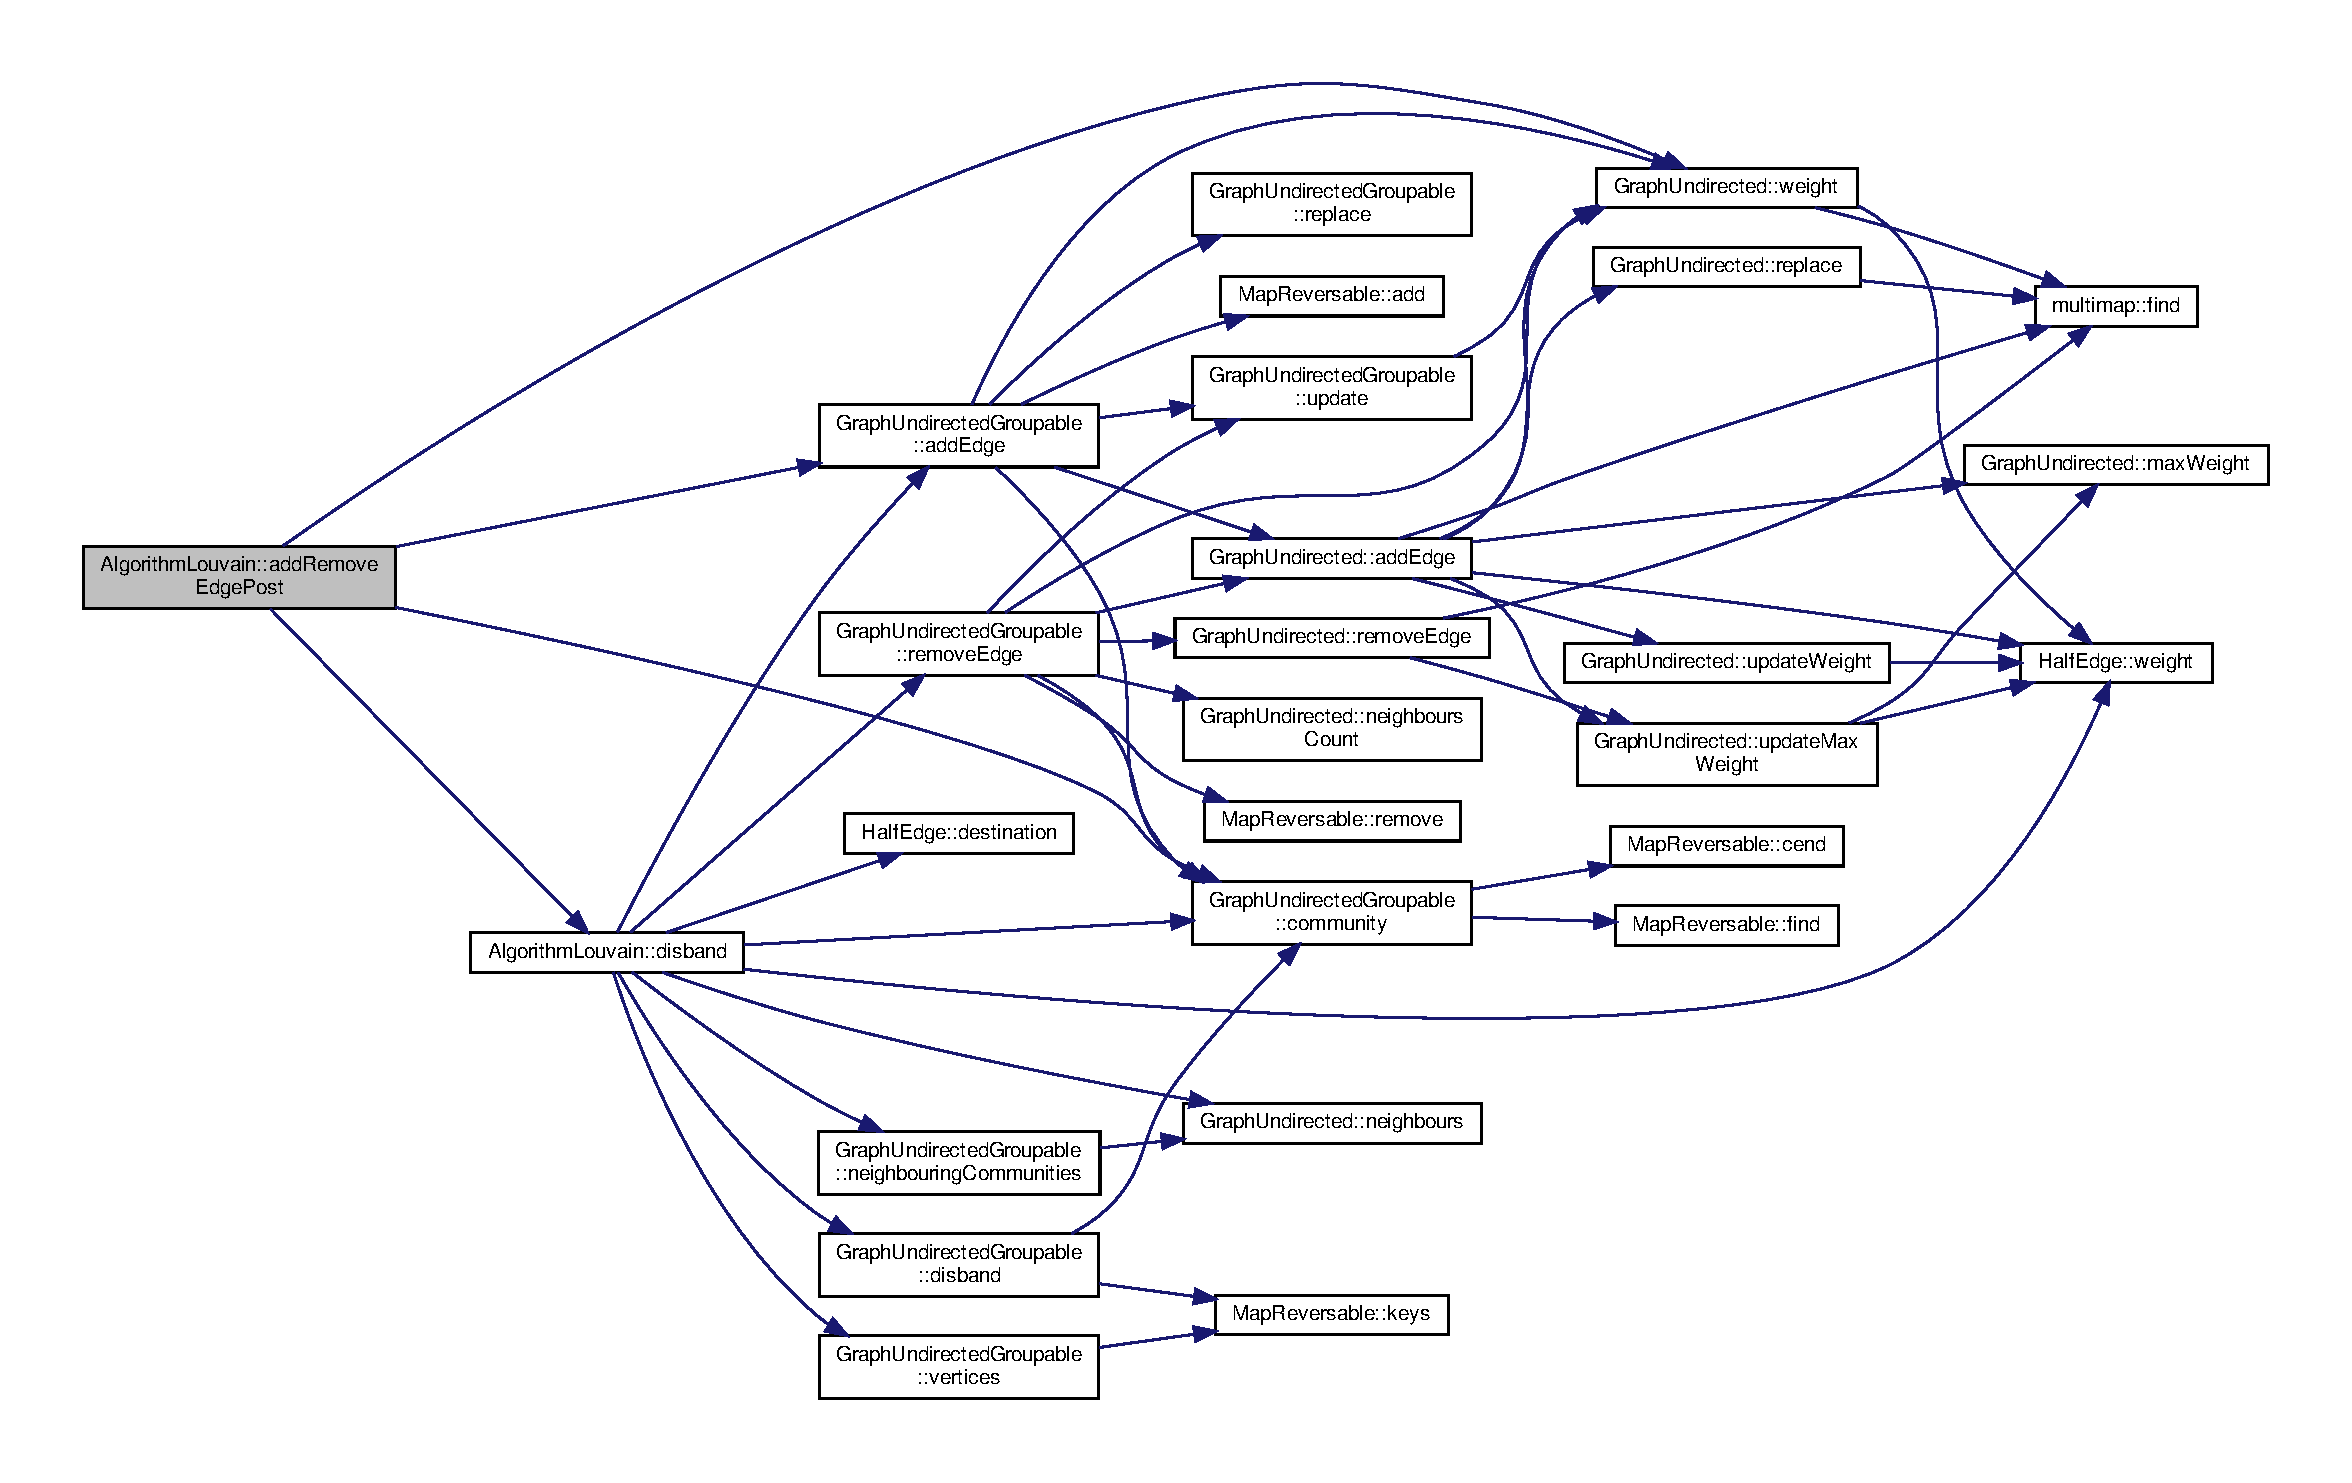
\includegraphics[width=350pt]{classAlgorithmLouvain_a69f296749859441c8a3844753bdd58e5_cgraph}
\end{center}
\end{figure}
\mbox{\Hypertarget{classAlgorithmLouvain_a883c922bf2f3c3aadb9db4962c0d8dce}\label{classAlgorithmLouvain_a883c922bf2f3c3aadb9db4962c0d8dce}} 
\index{Algorithm\+Louvain@{Algorithm\+Louvain}!add\+Remove\+Edge\+Pre@{add\+Remove\+Edge\+Pre}}
\index{add\+Remove\+Edge\+Pre@{add\+Remove\+Edge\+Pre}!Algorithm\+Louvain@{Algorithm\+Louvain}}
\subsubsection{\texorpdfstring{add\+Remove\+Edge\+Pre()}{addRemoveEdgePre()}}
{\footnotesize\ttfamily bool Algorithm\+Louvain\+::add\+Remove\+Edge\+Pre (\begin{DoxyParamCaption}\item[{const \hyperlink{edge_8h_a5fbd20c46956d479cb10afc9855223f6}{type\+Vertex} \&}]{source,  }\item[{const \hyperlink{edge_8h_a5fbd20c46956d479cb10afc9855223f6}{type\+Vertex} \&}]{destination,  }\item[{const \hyperlink{edge_8h_a2e7ea3be891ac8b52f749ec73fee6dd2}{type\+Weight} \&}]{weight = {\ttfamily 1.0} }\end{DoxyParamCaption})\hspace{0.3cm}{\ttfamily [inline]}, {\ttfamily [virtual]}}

Function to execute before adding or removing a single edge from the graph. It is used internally by the add\+Remove\+Edges function. Useful if pre-\/processing is required, for example, to update some of variables before the edge can be added or removed. Any edge with a weight different from zero is inserted. Any edge with a weight of exactly zero is removed.


\begin{DoxyParams}{Parameters}
{\em source} & source vertex \\
\hline
{\em destination} & destination vertex \\
\hline
{\em weight} & optional if adding an edge. Must be exactly zero to remove an edge. \\
\hline
\end{DoxyParams}
\begin{DoxyReturn}{Returns}
true if all operations succeeded. False, otherwise. 
\end{DoxyReturn}


Implements \hyperlink{classAlgorithmInterface_ae5a6e84b139768dff92a70cacaec7472}{Algorithm\+Interface}.



Definition at line 401 of file algorithm\+Louvain.\+h.



References Graph\+Undirected\+Groupable\+::add\+Edge(), Graph\+Undirected\+Groupable\+::community(), Algorithm\+Base\+::grph, Graph\+Undirected\+Groupable\+::remove\+Edge(), and Graph\+Undirected\+::weight().



Referenced by Algorithm\+::add\+Remove\+Edge\+Pre().

Here is the call graph for this function\+:
\nopagebreak
\begin{figure}[H]
\begin{center}
\leavevmode
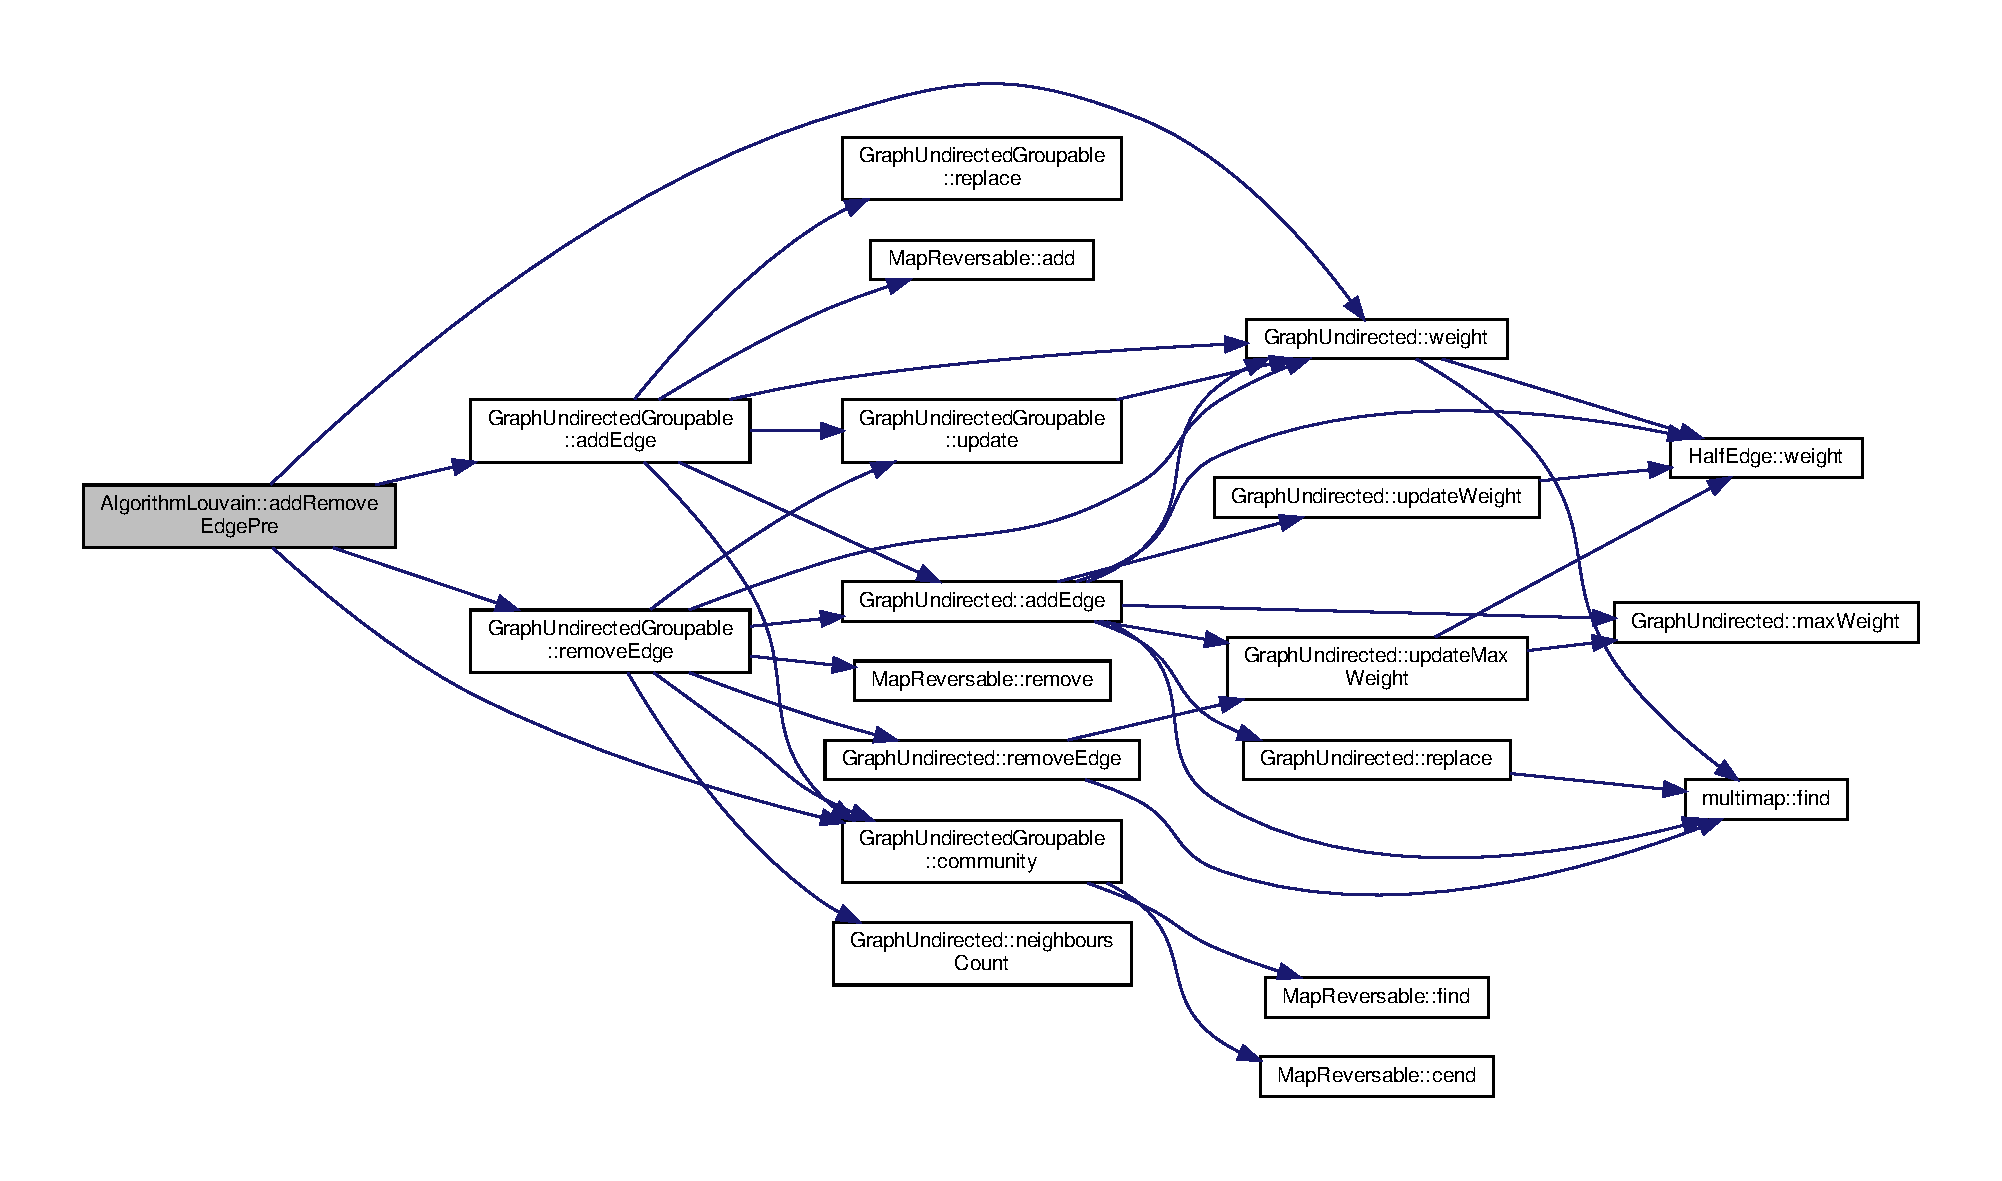
\includegraphics[width=350pt]{classAlgorithmLouvain_a883c922bf2f3c3aadb9db4962c0d8dce_cgraph}
\end{center}
\end{figure}
\mbox{\Hypertarget{classAlgorithmLouvain_a5f59777e27ab7a3e5accbc1f52b0e51e}\label{classAlgorithmLouvain_a5f59777e27ab7a3e5accbc1f52b0e51e}} 
\index{Algorithm\+Louvain@{Algorithm\+Louvain}!community@{community}}
\index{community@{community}!Algorithm\+Louvain@{Algorithm\+Louvain}}
\subsubsection{\texorpdfstring{community()}{community()}\hspace{0.1cm}{\footnotesize\ttfamily [1/2]}}
{\footnotesize\ttfamily const \hyperlink{graphUndirectedGroupable_8h_a914da95c9ea7f14f4b7f875c36818556}{type\+Community}\& Algorithm\+Louvain\+::community (\begin{DoxyParamCaption}\item[{const \hyperlink{edge_8h_a5fbd20c46956d479cb10afc9855223f6}{type\+Vertex} \&}]{node }\end{DoxyParamCaption}) const\hspace{0.3cm}{\ttfamily [inline]}, {\ttfamily [private]}}



Definition at line 65 of file algorithm\+Louvain.\+h.



References Graph\+Undirected\+Groupable\+::community(), Algorithm\+Base\+::grph, and no\+Group.



Referenced by neigh\+\_\+comm(), and one\+\_\+level().

Here is the call graph for this function\+:
\nopagebreak
\begin{figure}[H]
\begin{center}
\leavevmode
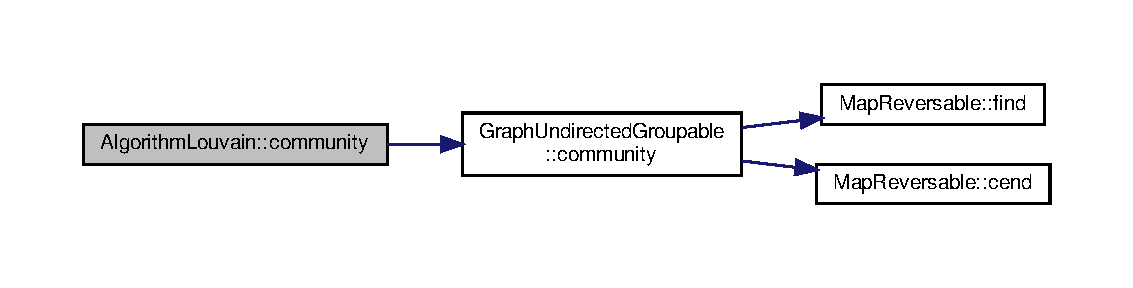
\includegraphics[width=350pt]{classAlgorithmLouvain_a5f59777e27ab7a3e5accbc1f52b0e51e_cgraph}
\end{center}
\end{figure}
\mbox{\Hypertarget{classAlgorithmLouvain_a12549c842a87a6f9380ee8226ac58cf8}\label{classAlgorithmLouvain_a12549c842a87a6f9380ee8226ac58cf8}} 
\index{Algorithm\+Louvain@{Algorithm\+Louvain}!community@{community}}
\index{community@{community}!Algorithm\+Louvain@{Algorithm\+Louvain}}
\subsubsection{\texorpdfstring{community()}{community()}\hspace{0.1cm}{\footnotesize\ttfamily [2/2]}}
{\footnotesize\ttfamily bool Algorithm\+Louvain\+::community (\begin{DoxyParamCaption}\item[{const \hyperlink{edge_8h_a5fbd20c46956d479cb10afc9855223f6}{type\+Vertex} \&}]{node,  }\item[{const \hyperlink{graphUndirectedGroupable_8h_a914da95c9ea7f14f4b7f875c36818556}{type\+Community} \&}]{com }\end{DoxyParamCaption})\hspace{0.3cm}{\ttfamily [inline]}, {\ttfamily [private]}}



Definition at line 73 of file algorithm\+Louvain.\+h.



References Graph\+Undirected\+Groupable\+::community(), and Algorithm\+Base\+::grph.

Here is the call graph for this function\+:
\nopagebreak
\begin{figure}[H]
\begin{center}
\leavevmode
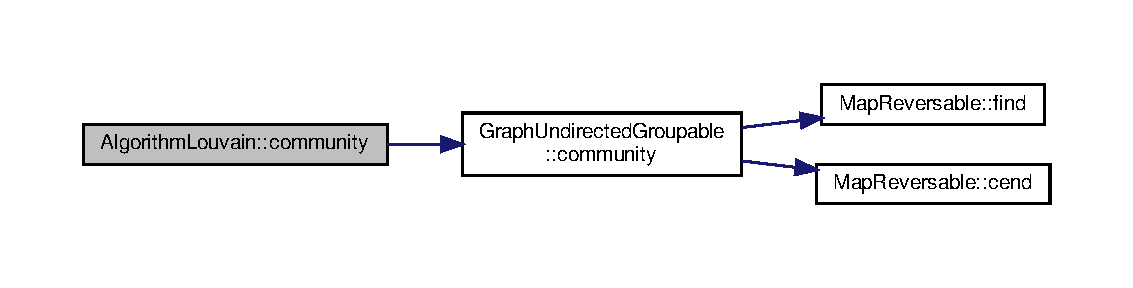
\includegraphics[width=350pt]{classAlgorithmLouvain_a12549c842a87a6f9380ee8226ac58cf8_cgraph}
\end{center}
\end{figure}
\mbox{\Hypertarget{classAlgorithmLouvain_a8a8af8c837dd1a24a6be7904121edbbd}\label{classAlgorithmLouvain_a8a8af8c837dd1a24a6be7904121edbbd}} 
\index{Algorithm\+Louvain@{Algorithm\+Louvain}!community\+Count@{community\+Count}}
\index{community\+Count@{community\+Count}!Algorithm\+Louvain@{Algorithm\+Louvain}}
\subsubsection{\texorpdfstring{community\+Count()}{communityCount()}}
{\footnotesize\ttfamily const \hyperlink{edge_8h_a2e7ea3be891ac8b52f749ec73fee6dd2}{type\+Weight} Algorithm\+Louvain\+::community\+Count (\begin{DoxyParamCaption}{ }\end{DoxyParamCaption}) const\hspace{0.3cm}{\ttfamily [inline]}, {\ttfamily [private]}}



Definition at line 152 of file algorithm\+Louvain.\+h.



References Graph\+Undirected\+Groupable\+::community\+Count(), and Algorithm\+Base\+::grph.

Here is the call graph for this function\+:
\nopagebreak
\begin{figure}[H]
\begin{center}
\leavevmode
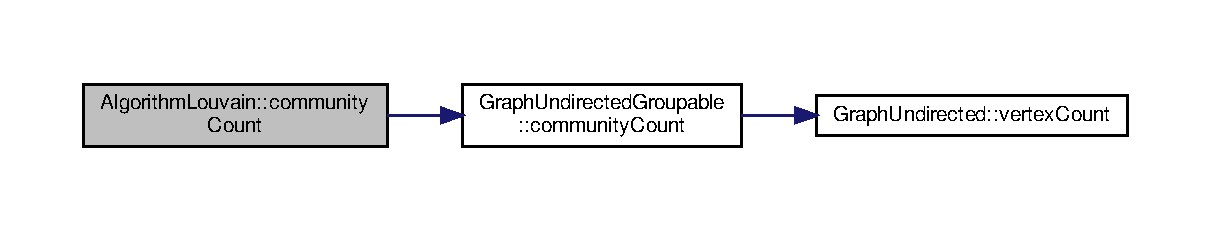
\includegraphics[width=350pt]{classAlgorithmLouvain_a8a8af8c837dd1a24a6be7904121edbbd_cgraph}
\end{center}
\end{figure}
\mbox{\Hypertarget{classAlgorithmLouvain_a1e38f3c6a2df8b028328131b3dfceb94}\label{classAlgorithmLouvain_a1e38f3c6a2df8b028328131b3dfceb94}} 
\index{Algorithm\+Louvain@{Algorithm\+Louvain}!disband@{disband}}
\index{disband@{disband}!Algorithm\+Louvain@{Algorithm\+Louvain}}
\subsubsection{\texorpdfstring{disband()}{disband()}}
{\footnotesize\ttfamily void Algorithm\+Louvain\+::disband (\begin{DoxyParamCaption}\item[{const \hyperlink{graphUndirectedGroupable_8h_a914da95c9ea7f14f4b7f875c36818556}{type\+Community}}]{c1,  }\item[{const \hyperlink{graphUndirectedGroupable_8h_a914da95c9ea7f14f4b7f875c36818556}{type\+Community}}]{c2 }\end{DoxyParamCaption})\hspace{0.3cm}{\ttfamily [inline]}, {\ttfamily [private]}}

Disband communities belonging to the given edge. Source and destination communities must be different. It is an algorithm requirement that, when adding edges, the communities involved get removed and replaced by their individual vertices, so that calculation are only performed over those vertices, making the Louvain algorithm dynamic. 
\begin{DoxyParams}{Parameters}
{\em c1} & the source community of the edge \\
\hline
{\em c2} & the destination community of the edge \\
\hline
\end{DoxyParams}


Definition at line 195 of file algorithm\+Louvain.\+h.



References Graph\+Undirected\+Groupable\+::add\+Edge(), Graph\+Undirected\+Groupable\+::community(), Half\+Edge\+::destination(), Graph\+Undirected\+Groupable\+::disband(), Algorithm\+Base\+::grph, Graph\+Undirected\+Groupable\+::neighbouring\+Communities(), Graph\+Undirected\+::neighbours(), Graph\+Undirected\+Groupable\+::remove\+Edge(), Graph\+Undirected\+Groupable\+::vertices(), and Half\+Edge\+::weight().



Referenced by add\+Remove\+Edge\+Post().

Here is the call graph for this function\+:
\nopagebreak
\begin{figure}[H]
\begin{center}
\leavevmode
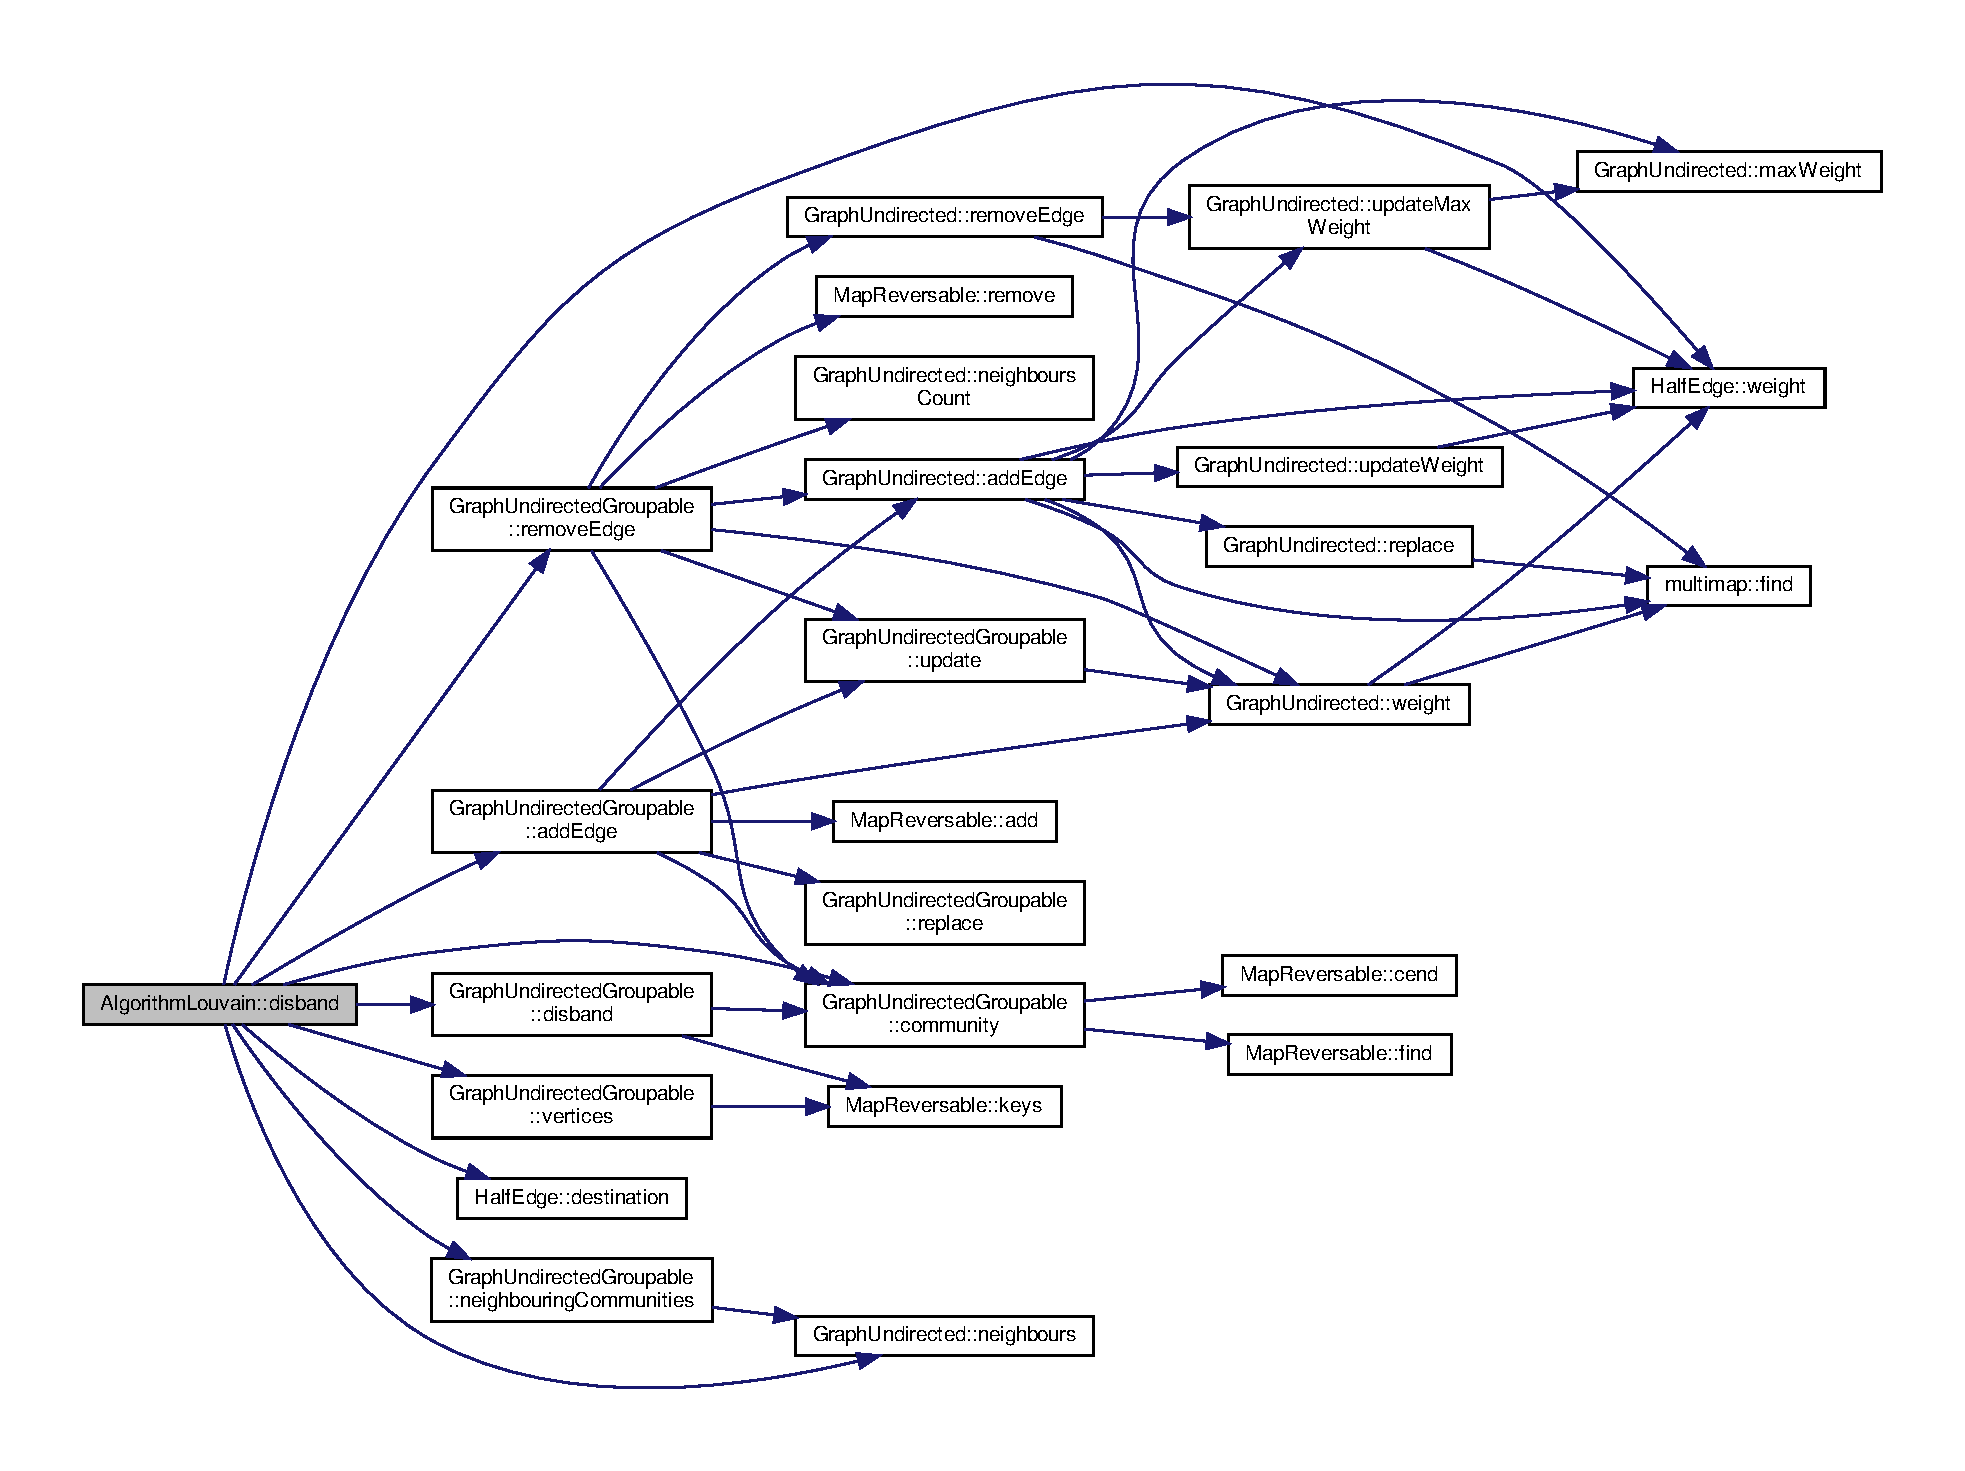
\includegraphics[width=350pt]{classAlgorithmLouvain_a1e38f3c6a2df8b028328131b3dfceb94_cgraph}
\end{center}
\end{figure}
\mbox{\Hypertarget{classAlgorithmLouvain_aa4b25143d94b4fabc830ea053b76dd7d}\label{classAlgorithmLouvain_aa4b25143d94b4fabc830ea053b76dd7d}} 
\index{Algorithm\+Louvain@{Algorithm\+Louvain}!edge\+Count@{edge\+Count}}
\index{edge\+Count@{edge\+Count}!Algorithm\+Louvain@{Algorithm\+Louvain}}
\subsubsection{\texorpdfstring{edge\+Count()}{edgeCount()}}
{\footnotesize\ttfamily const \hyperlink{edge_8h_a2e7ea3be891ac8b52f749ec73fee6dd2}{type\+Weight} Algorithm\+Louvain\+::edge\+Count (\begin{DoxyParamCaption}{ }\end{DoxyParamCaption}) const\hspace{0.3cm}{\ttfamily [inline]}, {\ttfamily [private]}}



Definition at line 147 of file algorithm\+Louvain.\+h.



References Graph\+Undirected\+::edge\+Count(), and Algorithm\+Base\+::grph.

Here is the call graph for this function\+:
\nopagebreak
\begin{figure}[H]
\begin{center}
\leavevmode
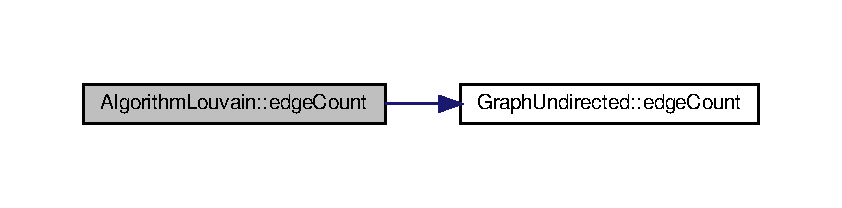
\includegraphics[width=350pt]{classAlgorithmLouvain_aa4b25143d94b4fabc830ea053b76dd7d_cgraph}
\end{center}
\end{figure}
\mbox{\Hypertarget{classAlgorithmLouvain_a6d5f1cfcbe2581bbe7bbe285392e0bdf}\label{classAlgorithmLouvain_a6d5f1cfcbe2581bbe7bbe285392e0bdf}} 
\index{Algorithm\+Louvain@{Algorithm\+Louvain}!edges@{edges}}
\index{edges@{edges}!Algorithm\+Louvain@{Algorithm\+Louvain}}
\subsubsection{\texorpdfstring{edges()}{edges()}}
{\footnotesize\ttfamily \hyperlink{graphInterface_8h_ae8d27008f15586bbf419af7ad2e0a48a}{type\+Links\+Range\+Const} Algorithm\+Louvain\+::edges (\begin{DoxyParamCaption}{ }\end{DoxyParamCaption}) const\hspace{0.3cm}{\ttfamily [inline]}, {\ttfamily [private]}}



Definition at line 92 of file algorithm\+Louvain.\+h.



References Graph\+Undirected\+::edges(), and Algorithm\+Base\+::grph.

Here is the call graph for this function\+:
\nopagebreak
\begin{figure}[H]
\begin{center}
\leavevmode
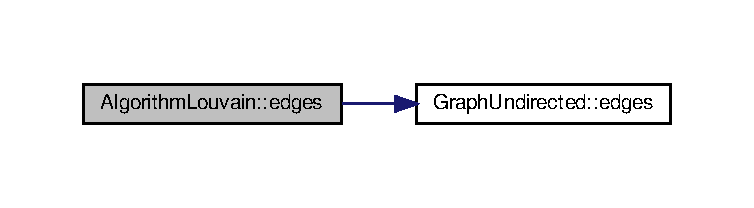
\includegraphics[width=350pt]{classAlgorithmLouvain_a6d5f1cfcbe2581bbe7bbe285392e0bdf_cgraph}
\end{center}
\end{figure}
\mbox{\Hypertarget{classAlgorithmLouvain_adcd4a8dc566881f9c1b1d9e78730a503}\label{classAlgorithmLouvain_adcd4a8dc566881f9c1b1d9e78730a503}} 
\index{Algorithm\+Louvain@{Algorithm\+Louvain}!gain@{gain}}
\index{gain@{gain}!Algorithm\+Louvain@{Algorithm\+Louvain}}
\subsubsection{\texorpdfstring{gain()}{gain()}}
{\footnotesize\ttfamily \hyperlink{criterionInterface_8h_af71ff22f6355fd69a4a62104bfd59a83}{type\+Criterion} Algorithm\+Louvain\+::gain (\begin{DoxyParamCaption}\item[{const \hyperlink{edge_8h_a5fbd20c46956d479cb10afc9855223f6}{type\+Vertex} \&}]{vertex,  }\item[{const \hyperlink{graphUndirectedGroupable_8h_a914da95c9ea7f14f4b7f875c36818556}{type\+Community} \&}]{comm }\end{DoxyParamCaption}) const\hspace{0.3cm}{\ttfamily [inline]}, {\ttfamily [private]}}



Definition at line 169 of file algorithm\+Louvain.\+h.



References Criterion\+::gain(), and Algorithm\+Base\+::qlt.



Referenced by one\+\_\+level().

Here is the call graph for this function\+:
\nopagebreak
\begin{figure}[H]
\begin{center}
\leavevmode
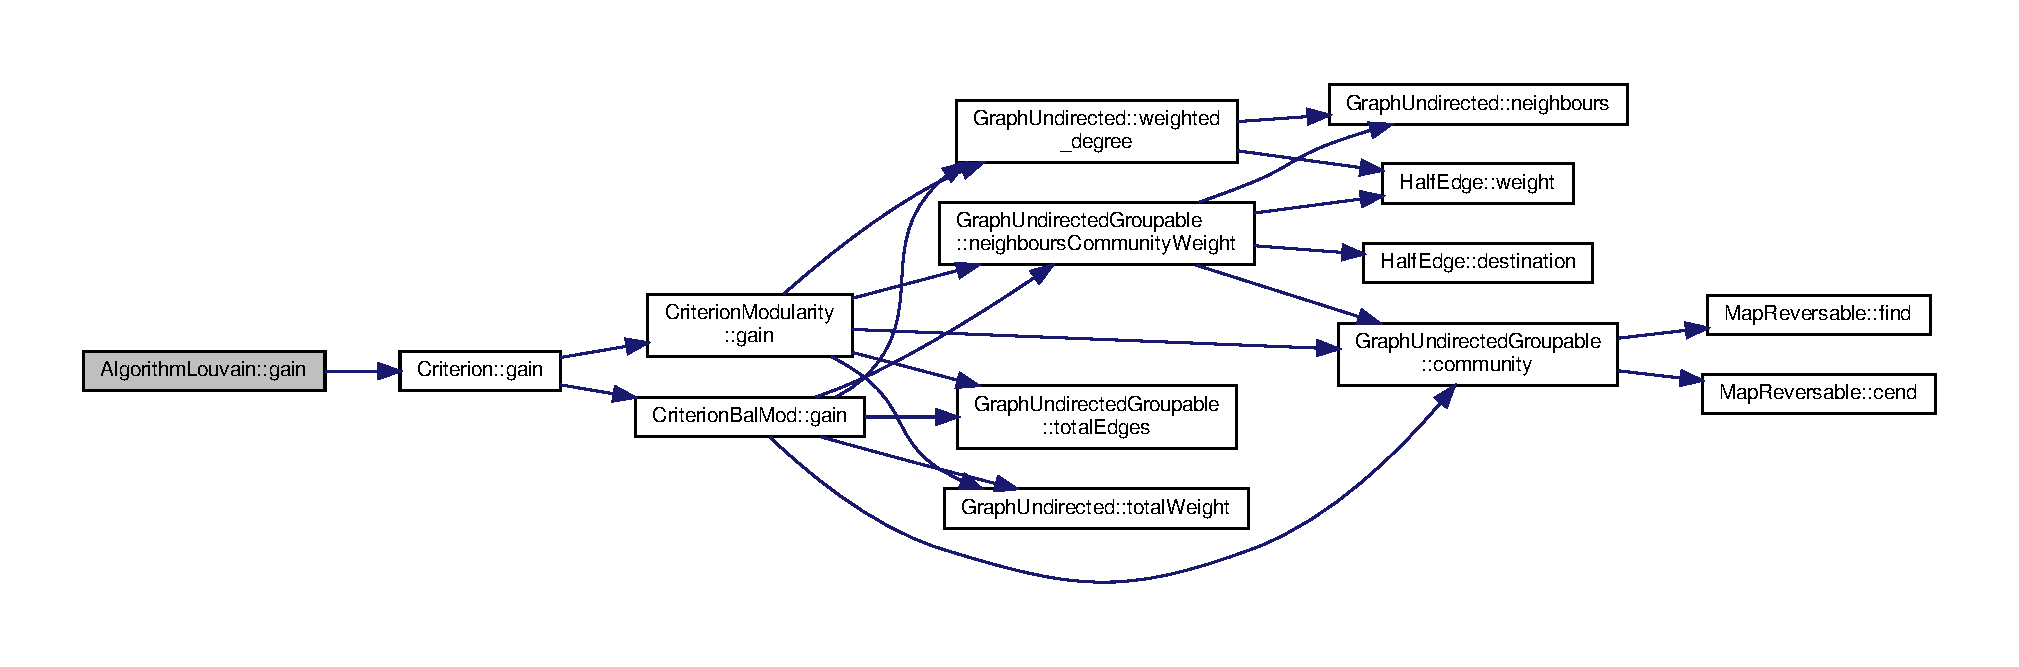
\includegraphics[width=350pt]{classAlgorithmLouvain_adcd4a8dc566881f9c1b1d9e78730a503_cgraph}
\end{center}
\end{figure}
\mbox{\Hypertarget{classAlgorithmLouvain_a627618ba516be4f4906143b6b0ff1c77}\label{classAlgorithmLouvain_a627618ba516be4f4906143b6b0ff1c77}} 
\index{Algorithm\+Louvain@{Algorithm\+Louvain}!get\+Vertices@{get\+Vertices}}
\index{get\+Vertices@{get\+Vertices}!Algorithm\+Louvain@{Algorithm\+Louvain}}
\subsubsection{\texorpdfstring{get\+Vertices()}{getVertices()}}
{\footnotesize\ttfamily const \hyperlink{graphInterface_8h_a21d54d8a139def524d3b0d6f71ec4974}{type\+Vertex\+List}\& Algorithm\+Louvain\+::get\+Vertices (\begin{DoxyParamCaption}{ }\end{DoxyParamCaption}) const\hspace{0.3cm}{\ttfamily [inline]}, {\ttfamily [private]}}



Definition at line 97 of file algorithm\+Louvain.\+h.



References Graph\+Undirected\+::get\+Vertices(), and Algorithm\+Base\+::grph.



Referenced by one\+\_\+level().

Here is the call graph for this function\+:
\nopagebreak
\begin{figure}[H]
\begin{center}
\leavevmode
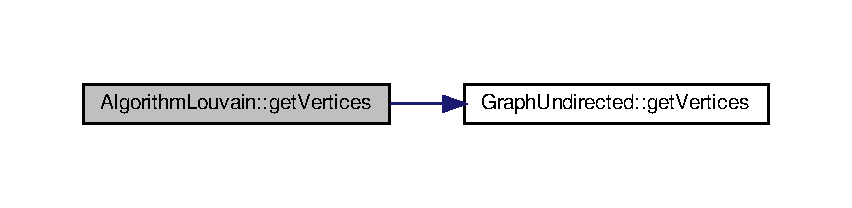
\includegraphics[width=350pt]{classAlgorithmLouvain_a627618ba516be4f4906143b6b0ff1c77_cgraph}
\end{center}
\end{figure}
\mbox{\Hypertarget{classAlgorithmLouvain_a066612d0b1d64d8f5c7d84f20bbf70c4}\label{classAlgorithmLouvain_a066612d0b1d64d8f5c7d84f20bbf70c4}} 
\index{Algorithm\+Louvain@{Algorithm\+Louvain}!inner\+Edges@{inner\+Edges}}
\index{inner\+Edges@{inner\+Edges}!Algorithm\+Louvain@{Algorithm\+Louvain}}
\subsubsection{\texorpdfstring{inner\+Edges()}{innerEdges()}}
{\footnotesize\ttfamily \hyperlink{edge_8h_a2e7ea3be891ac8b52f749ec73fee6dd2}{type\+Weight} Algorithm\+Louvain\+::inner\+Edges (\begin{DoxyParamCaption}\item[{const \hyperlink{graphUndirectedGroupable_8h_a914da95c9ea7f14f4b7f875c36818556}{type\+Community} \&}]{c }\end{DoxyParamCaption}) const\hspace{0.3cm}{\ttfamily [inline]}, {\ttfamily [private]}}



Definition at line 82 of file algorithm\+Louvain.\+h.



References Algorithm\+Base\+::grph, and Graph\+Undirected\+Groupable\+::inner\+Edges().

Here is the call graph for this function\+:
\nopagebreak
\begin{figure}[H]
\begin{center}
\leavevmode
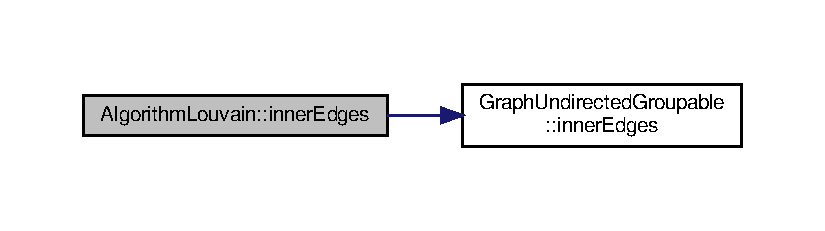
\includegraphics[width=350pt]{classAlgorithmLouvain_a066612d0b1d64d8f5c7d84f20bbf70c4_cgraph}
\end{center}
\end{figure}
\mbox{\Hypertarget{classAlgorithmLouvain_a0b2ef33d5d1bf8b9aa2f8c73921844ac}\label{classAlgorithmLouvain_a0b2ef33d5d1bf8b9aa2f8c73921844ac}} 
\index{Algorithm\+Louvain@{Algorithm\+Louvain}!max\+Weight@{max\+Weight}}
\index{max\+Weight@{max\+Weight}!Algorithm\+Louvain@{Algorithm\+Louvain}}
\subsubsection{\texorpdfstring{max\+Weight()}{maxWeight()}}
{\footnotesize\ttfamily const \hyperlink{edge_8h_a2e7ea3be891ac8b52f749ec73fee6dd2}{type\+Weight}\& Algorithm\+Louvain\+::max\+Weight (\begin{DoxyParamCaption}{ }\end{DoxyParamCaption}) const\hspace{0.3cm}{\ttfamily [inline]}, {\ttfamily [private]}}



Definition at line 132 of file algorithm\+Louvain.\+h.



References Algorithm\+Base\+::grph, and Graph\+Undirected\+::max\+Weight().

Here is the call graph for this function\+:
\nopagebreak
\begin{figure}[H]
\begin{center}
\leavevmode
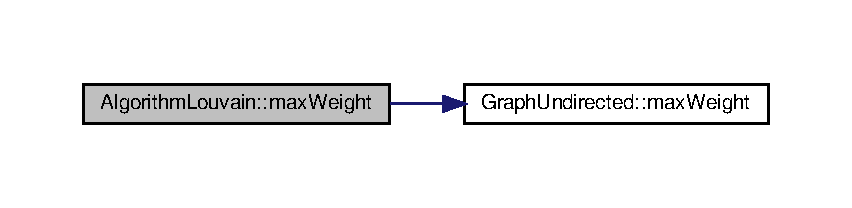
\includegraphics[width=350pt]{classAlgorithmLouvain_a0b2ef33d5d1bf8b9aa2f8c73921844ac_cgraph}
\end{center}
\end{figure}
\mbox{\Hypertarget{classAlgorithmLouvain_a78dfa81bd96f4036e44c17318501b6b7}\label{classAlgorithmLouvain_a78dfa81bd96f4036e44c17318501b6b7}} 
\index{Algorithm\+Louvain@{Algorithm\+Louvain}!neigh\+\_\+comm@{neigh\+\_\+comm}}
\index{neigh\+\_\+comm@{neigh\+\_\+comm}!Algorithm\+Louvain@{Algorithm\+Louvain}}
\subsubsection{\texorpdfstring{neigh\+\_\+comm()}{neigh\_comm()}}
{\footnotesize\ttfamily std\+::map$<$\hyperlink{graphUndirectedGroupable_8h_a914da95c9ea7f14f4b7f875c36818556}{type\+Community}, \hyperlink{edge_8h_a2e7ea3be891ac8b52f749ec73fee6dd2}{type\+Weight}$>$ Algorithm\+Louvain\+::neigh\+\_\+comm (\begin{DoxyParamCaption}\item[{const \hyperlink{edge_8h_a5fbd20c46956d479cb10afc9855223f6}{type\+Vertex} \&}]{vertex }\end{DoxyParamCaption}) const\hspace{0.3cm}{\ttfamily [inline]}, {\ttfamily [private]}}

Get the neighbouring communities of the given vertex with edge weight


\begin{DoxyParams}{Parameters}
{\em vertex} & \\
\hline
\end{DoxyParams}
\begin{DoxyReturn}{Returns}
the neighbouring communities of the given vertex 
\end{DoxyReturn}


Definition at line 266 of file algorithm\+Louvain.\+h.



References community(), Half\+Edge\+::destination(), neighbours(), no\+Vertex, and Half\+Edge\+::weight().



Referenced by one\+\_\+level().

Here is the call graph for this function\+:
\nopagebreak
\begin{figure}[H]
\begin{center}
\leavevmode
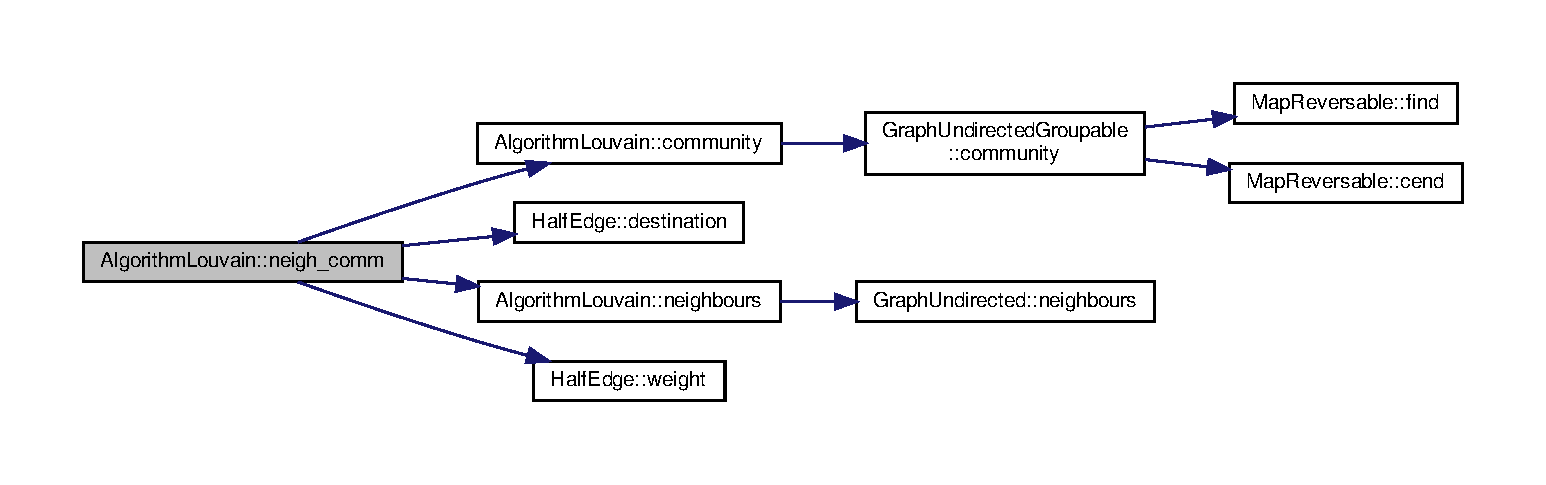
\includegraphics[width=350pt]{classAlgorithmLouvain_a78dfa81bd96f4036e44c17318501b6b7_cgraph}
\end{center}
\end{figure}
\mbox{\Hypertarget{classAlgorithmLouvain_ab6206bfc3cf537277c6965bc0da6d695}\label{classAlgorithmLouvain_ab6206bfc3cf537277c6965bc0da6d695}} 
\index{Algorithm\+Louvain@{Algorithm\+Louvain}!neighbours@{neighbours}}
\index{neighbours@{neighbours}!Algorithm\+Louvain@{Algorithm\+Louvain}}
\subsubsection{\texorpdfstring{neighbours()}{neighbours()}}
{\footnotesize\ttfamily \hyperlink{graphInterface_8h_ae8d27008f15586bbf419af7ad2e0a48a}{type\+Links\+Range\+Const} Algorithm\+Louvain\+::neighbours (\begin{DoxyParamCaption}\item[{const \hyperlink{edge_8h_a5fbd20c46956d479cb10afc9855223f6}{type\+Vertex} \&}]{node }\end{DoxyParamCaption}) const\hspace{0.3cm}{\ttfamily [inline]}, {\ttfamily [private]}}



Definition at line 107 of file algorithm\+Louvain.\+h.



References Algorithm\+Base\+::grph, and Graph\+Undirected\+::neighbours().



Referenced by neigh\+\_\+comm(), and one\+\_\+level().

Here is the call graph for this function\+:
\nopagebreak
\begin{figure}[H]
\begin{center}
\leavevmode
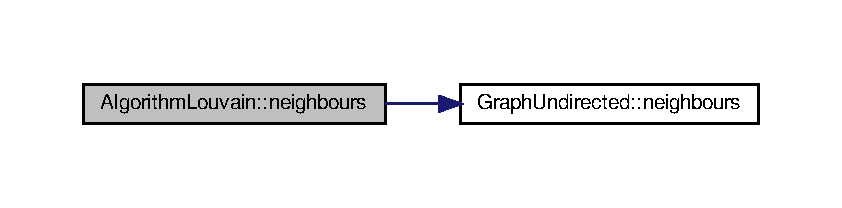
\includegraphics[width=350pt]{classAlgorithmLouvain_ab6206bfc3cf537277c6965bc0da6d695_cgraph}
\end{center}
\end{figure}
\mbox{\Hypertarget{classAlgorithmLouvain_a1d8b2b22ab5f49b08141696712baf337}\label{classAlgorithmLouvain_a1d8b2b22ab5f49b08141696712baf337}} 
\index{Algorithm\+Louvain@{Algorithm\+Louvain}!neighbours\+Community\+Count@{neighbours\+Community\+Count}}
\index{neighbours\+Community\+Count@{neighbours\+Community\+Count}!Algorithm\+Louvain@{Algorithm\+Louvain}}
\subsubsection{\texorpdfstring{neighbours\+Community\+Count()}{neighboursCommunityCount()}}
{\footnotesize\ttfamily unsigned int Algorithm\+Louvain\+::neighbours\+Community\+Count (\begin{DoxyParamCaption}\item[{const \hyperlink{edge_8h_a5fbd20c46956d479cb10afc9855223f6}{type\+Vertex} \&}]{node }\end{DoxyParamCaption}) const\hspace{0.3cm}{\ttfamily [inline]}, {\ttfamily [private]}}



Definition at line 117 of file algorithm\+Louvain.\+h.



References Algorithm\+Base\+::grph, and Graph\+Undirected\+Groupable\+::neighbours\+Community\+Count().

Here is the call graph for this function\+:
\nopagebreak
\begin{figure}[H]
\begin{center}
\leavevmode
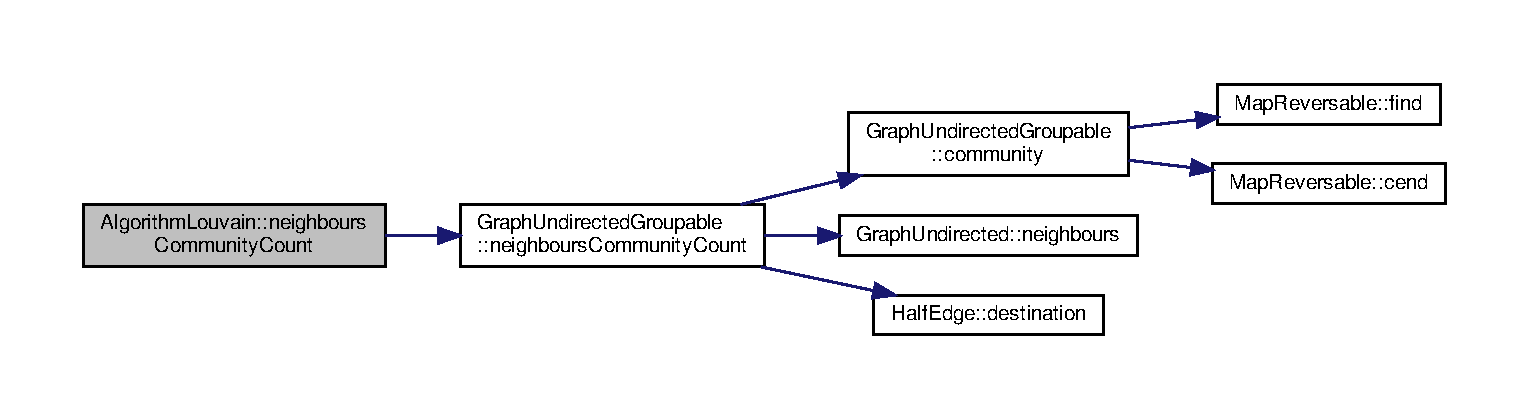
\includegraphics[width=350pt]{classAlgorithmLouvain_a1d8b2b22ab5f49b08141696712baf337_cgraph}
\end{center}
\end{figure}
\mbox{\Hypertarget{classAlgorithmLouvain_a4f1160234f469ddc9205e4d1217478ac}\label{classAlgorithmLouvain_a4f1160234f469ddc9205e4d1217478ac}} 
\index{Algorithm\+Louvain@{Algorithm\+Louvain}!neighbours\+Community\+Weight@{neighbours\+Community\+Weight}}
\index{neighbours\+Community\+Weight@{neighbours\+Community\+Weight}!Algorithm\+Louvain@{Algorithm\+Louvain}}
\subsubsection{\texorpdfstring{neighbours\+Community\+Weight()}{neighboursCommunityWeight()}\hspace{0.1cm}{\footnotesize\ttfamily [1/2]}}
{\footnotesize\ttfamily \hyperlink{edge_8h_a2e7ea3be891ac8b52f749ec73fee6dd2}{type\+Weight} Algorithm\+Louvain\+::neighbours\+Community\+Weight (\begin{DoxyParamCaption}\item[{const \hyperlink{edge_8h_a5fbd20c46956d479cb10afc9855223f6}{type\+Vertex} \&}]{node,  }\item[{const \hyperlink{graphUndirectedGroupable_8h_a914da95c9ea7f14f4b7f875c36818556}{type\+Community} \&}]{com }\end{DoxyParamCaption})\hspace{0.3cm}{\ttfamily [inline]}, {\ttfamily [private]}}



Definition at line 122 of file algorithm\+Louvain.\+h.



References Algorithm\+Base\+::grph, and Graph\+Undirected\+Groupable\+::neighbours\+Community\+Weight().

Here is the call graph for this function\+:
\nopagebreak
\begin{figure}[H]
\begin{center}
\leavevmode
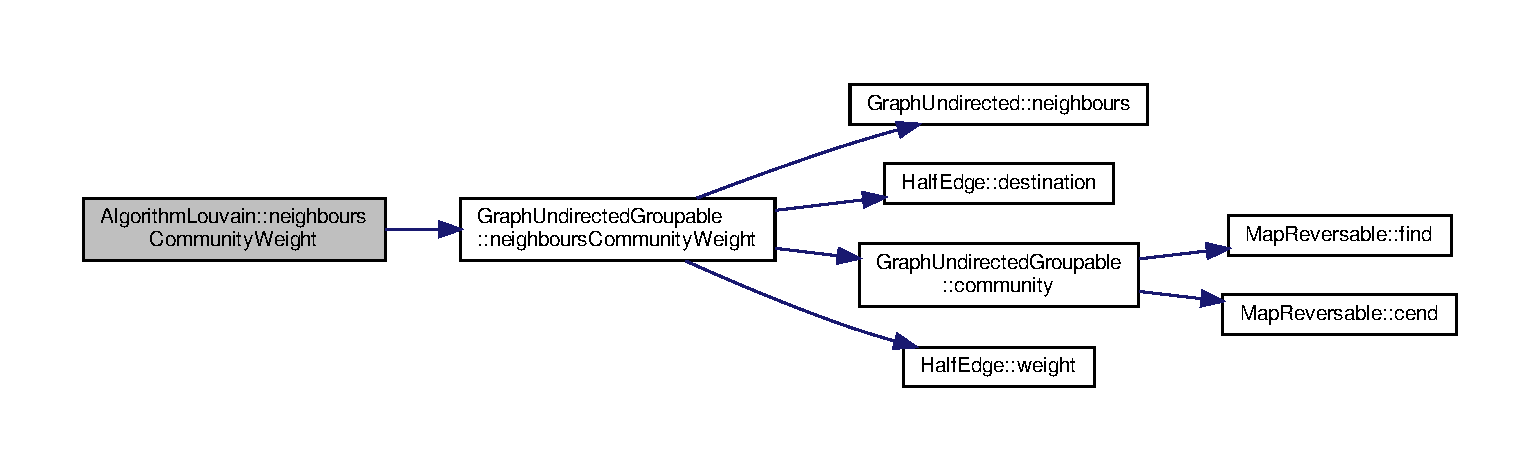
\includegraphics[width=350pt]{classAlgorithmLouvain_a4f1160234f469ddc9205e4d1217478ac_cgraph}
\end{center}
\end{figure}
\mbox{\Hypertarget{classAlgorithmLouvain_afc30a152fabdd874d45a0728ada4ec6e}\label{classAlgorithmLouvain_afc30a152fabdd874d45a0728ada4ec6e}} 
\index{Algorithm\+Louvain@{Algorithm\+Louvain}!neighbours\+Community\+Weight@{neighbours\+Community\+Weight}}
\index{neighbours\+Community\+Weight@{neighbours\+Community\+Weight}!Algorithm\+Louvain@{Algorithm\+Louvain}}
\subsubsection{\texorpdfstring{neighbours\+Community\+Weight()}{neighboursCommunityWeight()}\hspace{0.1cm}{\footnotesize\ttfamily [2/2]}}
{\footnotesize\ttfamily \hyperlink{edge_8h_a2e7ea3be891ac8b52f749ec73fee6dd2}{type\+Weight} Algorithm\+Louvain\+::neighbours\+Community\+Weight (\begin{DoxyParamCaption}\item[{const \hyperlink{edge_8h_a5fbd20c46956d479cb10afc9855223f6}{type\+Vertex} \&}]{node }\end{DoxyParamCaption})\hspace{0.3cm}{\ttfamily [inline]}, {\ttfamily [private]}}



Definition at line 127 of file algorithm\+Louvain.\+h.



References Algorithm\+Base\+::grph, and Graph\+Undirected\+Groupable\+::neighbours\+Community\+Weight().

Here is the call graph for this function\+:
\nopagebreak
\begin{figure}[H]
\begin{center}
\leavevmode
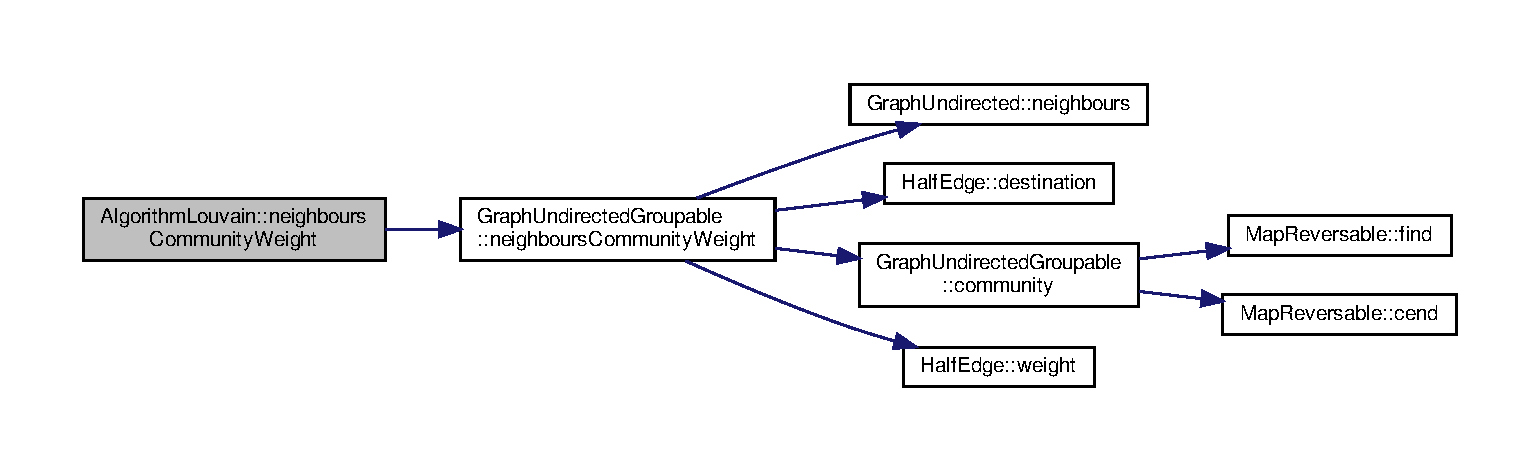
\includegraphics[width=350pt]{classAlgorithmLouvain_afc30a152fabdd874d45a0728ada4ec6e_cgraph}
\end{center}
\end{figure}
\mbox{\Hypertarget{classAlgorithmLouvain_ae0355167afc6ba8296f213469f6da4b0}\label{classAlgorithmLouvain_ae0355167afc6ba8296f213469f6da4b0}} 
\index{Algorithm\+Louvain@{Algorithm\+Louvain}!neighbours\+Count@{neighbours\+Count}}
\index{neighbours\+Count@{neighbours\+Count}!Algorithm\+Louvain@{Algorithm\+Louvain}}
\subsubsection{\texorpdfstring{neighbours\+Count()}{neighboursCount()}}
{\footnotesize\ttfamily unsigned int Algorithm\+Louvain\+::neighbours\+Count (\begin{DoxyParamCaption}\item[{const \hyperlink{edge_8h_a5fbd20c46956d479cb10afc9855223f6}{type\+Vertex} \&}]{node }\end{DoxyParamCaption}) const\hspace{0.3cm}{\ttfamily [inline]}, {\ttfamily [private]}}



Definition at line 112 of file algorithm\+Louvain.\+h.



References Algorithm\+Base\+::grph, and Graph\+Undirected\+::neighbours\+Count().

Here is the call graph for this function\+:
\nopagebreak
\begin{figure}[H]
\begin{center}
\leavevmode
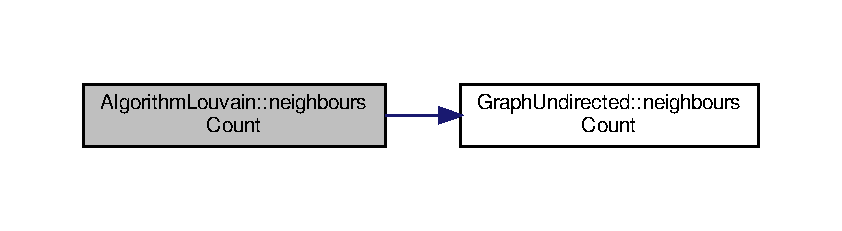
\includegraphics[width=350pt]{classAlgorithmLouvain_ae0355167afc6ba8296f213469f6da4b0_cgraph}
\end{center}
\end{figure}
\mbox{\Hypertarget{classAlgorithmLouvain_a5370c76e777b7cbfddd1dccd865d9356}\label{classAlgorithmLouvain_a5370c76e777b7cbfddd1dccd865d9356}} 
\index{Algorithm\+Louvain@{Algorithm\+Louvain}!one\+\_\+level@{one\+\_\+level}}
\index{one\+\_\+level@{one\+\_\+level}!Algorithm\+Louvain@{Algorithm\+Louvain}}
\subsubsection{\texorpdfstring{one\+\_\+level()}{one\_level()}}
{\footnotesize\ttfamily bool Algorithm\+Louvain\+::one\+\_\+level (\begin{DoxyParamCaption}{ }\end{DoxyParamCaption})\hspace{0.3cm}{\ttfamily [inline]}, {\ttfamily [private]}}

Function where the actual algorithm is implemented

\begin{DoxyReturn}{Returns}
true if there was an improvement in quality. False, otherwise 
\end{DoxyReturn}


Definition at line 294 of file algorithm\+Louvain.\+h.



References Graph\+Undirected\+Groupable\+::add\+Edge(), Graph\+Undirected\+Groupable\+::communities(), Graph\+Undirected\+Groupable\+::communities\+To\+Graph(), community(), Graph\+Undirected\+Groupable\+::community(), Half\+Edge\+::destination(), gain(), get\+Vertices(), Graph\+Undirected\+::get\+Vertices(), Algorithm\+Base\+::grph, Graph\+Undirected\+Groupable\+::inner\+Edges(), neigh\+\_\+comm(), Graph\+Undirected\+Groupable\+::neighbouring\+Communities(), neighbours(), Program\+Parameters\+::precision, Algorithm\+Base\+::prmtrs, quality(), Graph\+Undirected\+Groupable\+::vertices(), and Half\+Edge\+::weight().



Referenced by run().

Here is the call graph for this function\+:
\nopagebreak
\begin{figure}[H]
\begin{center}
\leavevmode
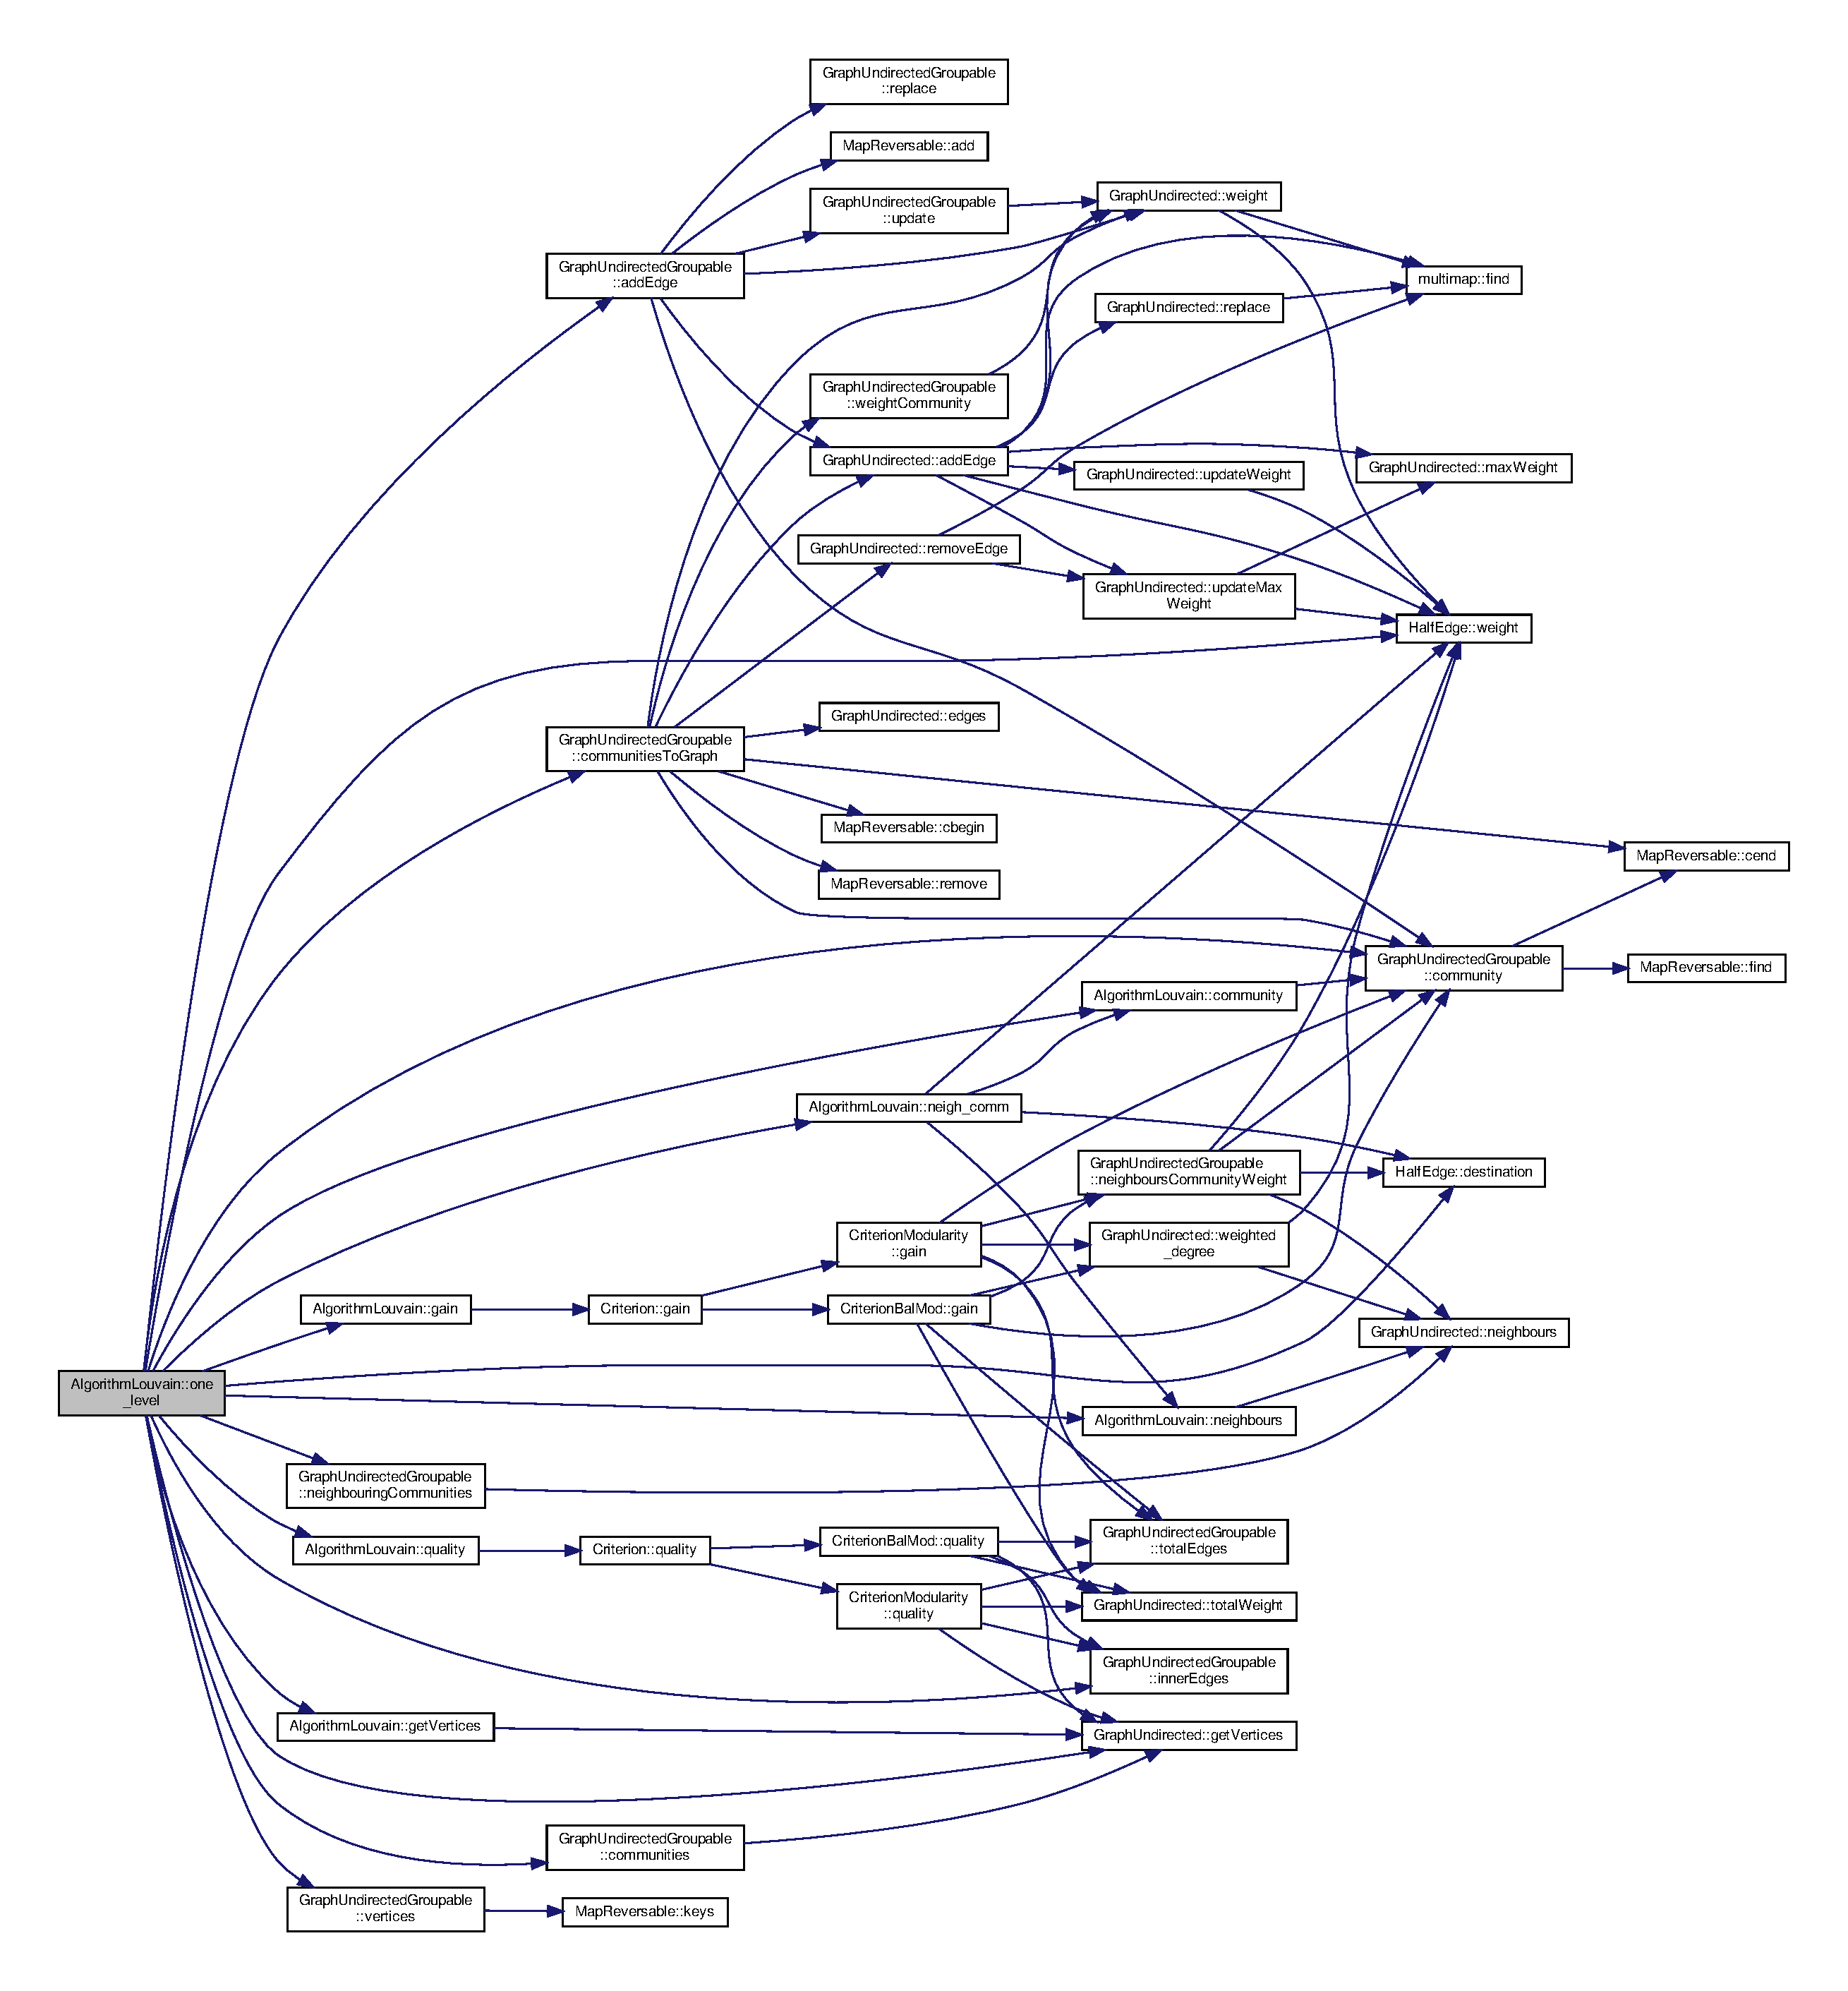
\includegraphics[width=350pt]{classAlgorithmLouvain_a5370c76e777b7cbfddd1dccd865d9356_cgraph}
\end{center}
\end{figure}
\mbox{\Hypertarget{classAlgorithmLouvain_a8c9b7694fff17eb5d8044cd26d7914e7}\label{classAlgorithmLouvain_a8c9b7694fff17eb5d8044cd26d7914e7}} 
\index{Algorithm\+Louvain@{Algorithm\+Louvain}!quality@{quality}}
\index{quality@{quality}!Algorithm\+Louvain@{Algorithm\+Louvain}}
\subsubsection{\texorpdfstring{quality()}{quality()}}
{\footnotesize\ttfamily \hyperlink{criterionInterface_8h_af71ff22f6355fd69a4a62104bfd59a83}{type\+Criterion} Algorithm\+Louvain\+::quality (\begin{DoxyParamCaption}{ }\end{DoxyParamCaption}) const\hspace{0.3cm}{\ttfamily [inline]}, {\ttfamily [private]}}



Definition at line 174 of file algorithm\+Louvain.\+h.



References Algorithm\+Base\+::qlt, and Criterion\+::quality().



Referenced by one\+\_\+level().

Here is the call graph for this function\+:
\nopagebreak
\begin{figure}[H]
\begin{center}
\leavevmode
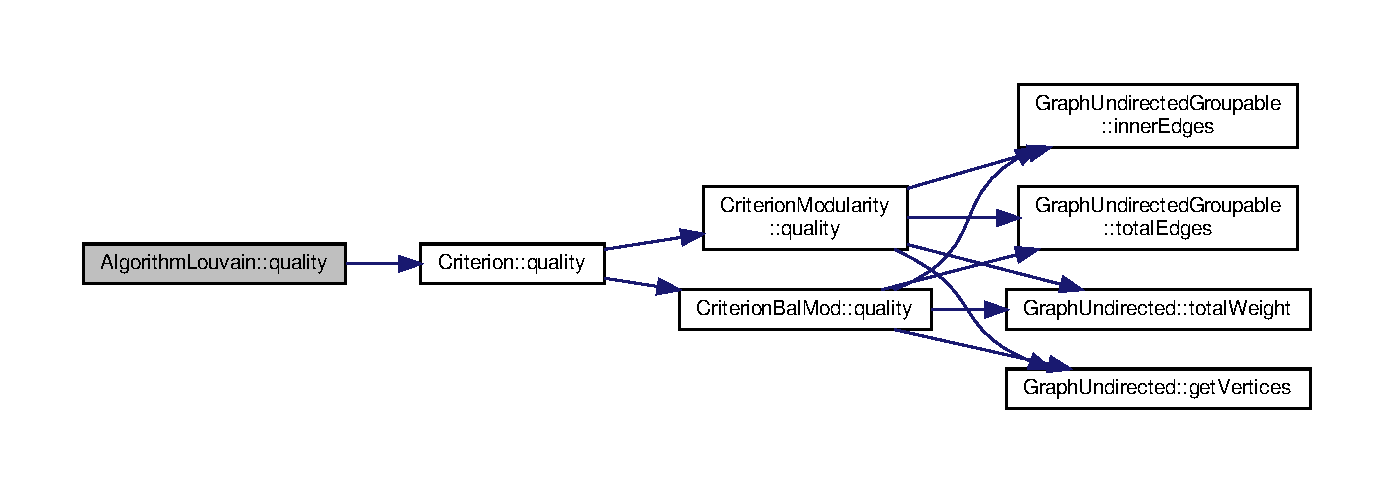
\includegraphics[width=350pt]{classAlgorithmLouvain_a8c9b7694fff17eb5d8044cd26d7914e7_cgraph}
\end{center}
\end{figure}
\mbox{\Hypertarget{classAlgorithmLouvain_a0a72b9dda25c69d19996dc7448924c13}\label{classAlgorithmLouvain_a0a72b9dda25c69d19996dc7448924c13}} 
\index{Algorithm\+Louvain@{Algorithm\+Louvain}!run@{run}}
\index{run@{run}!Algorithm\+Louvain@{Algorithm\+Louvain}}
\subsubsection{\texorpdfstring{run()}{run()}}
{\footnotesize\ttfamily bool Algorithm\+Louvain\+::run (\begin{DoxyParamCaption}{ }\end{DoxyParamCaption})\hspace{0.3cm}{\ttfamily [inline]}, {\ttfamily [virtual]}}

Function where the actual algorithms are implemented. It is called at the end of the add\+Remove\+Edges function.

\begin{DoxyReturn}{Returns}
true if all operations succeeded. False, otherwise. 
\end{DoxyReturn}


Implements \hyperlink{classAlgorithmInterface_a0bafcdabd2b5fd45abe97af91e02ca14}{Algorithm\+Interface}.



Definition at line 474 of file algorithm\+Louvain.\+h.



References Algorithm\+Louvain(), and one\+\_\+level().



Referenced by Algorithm\+::run().

Here is the call graph for this function\+:
\nopagebreak
\begin{figure}[H]
\begin{center}
\leavevmode
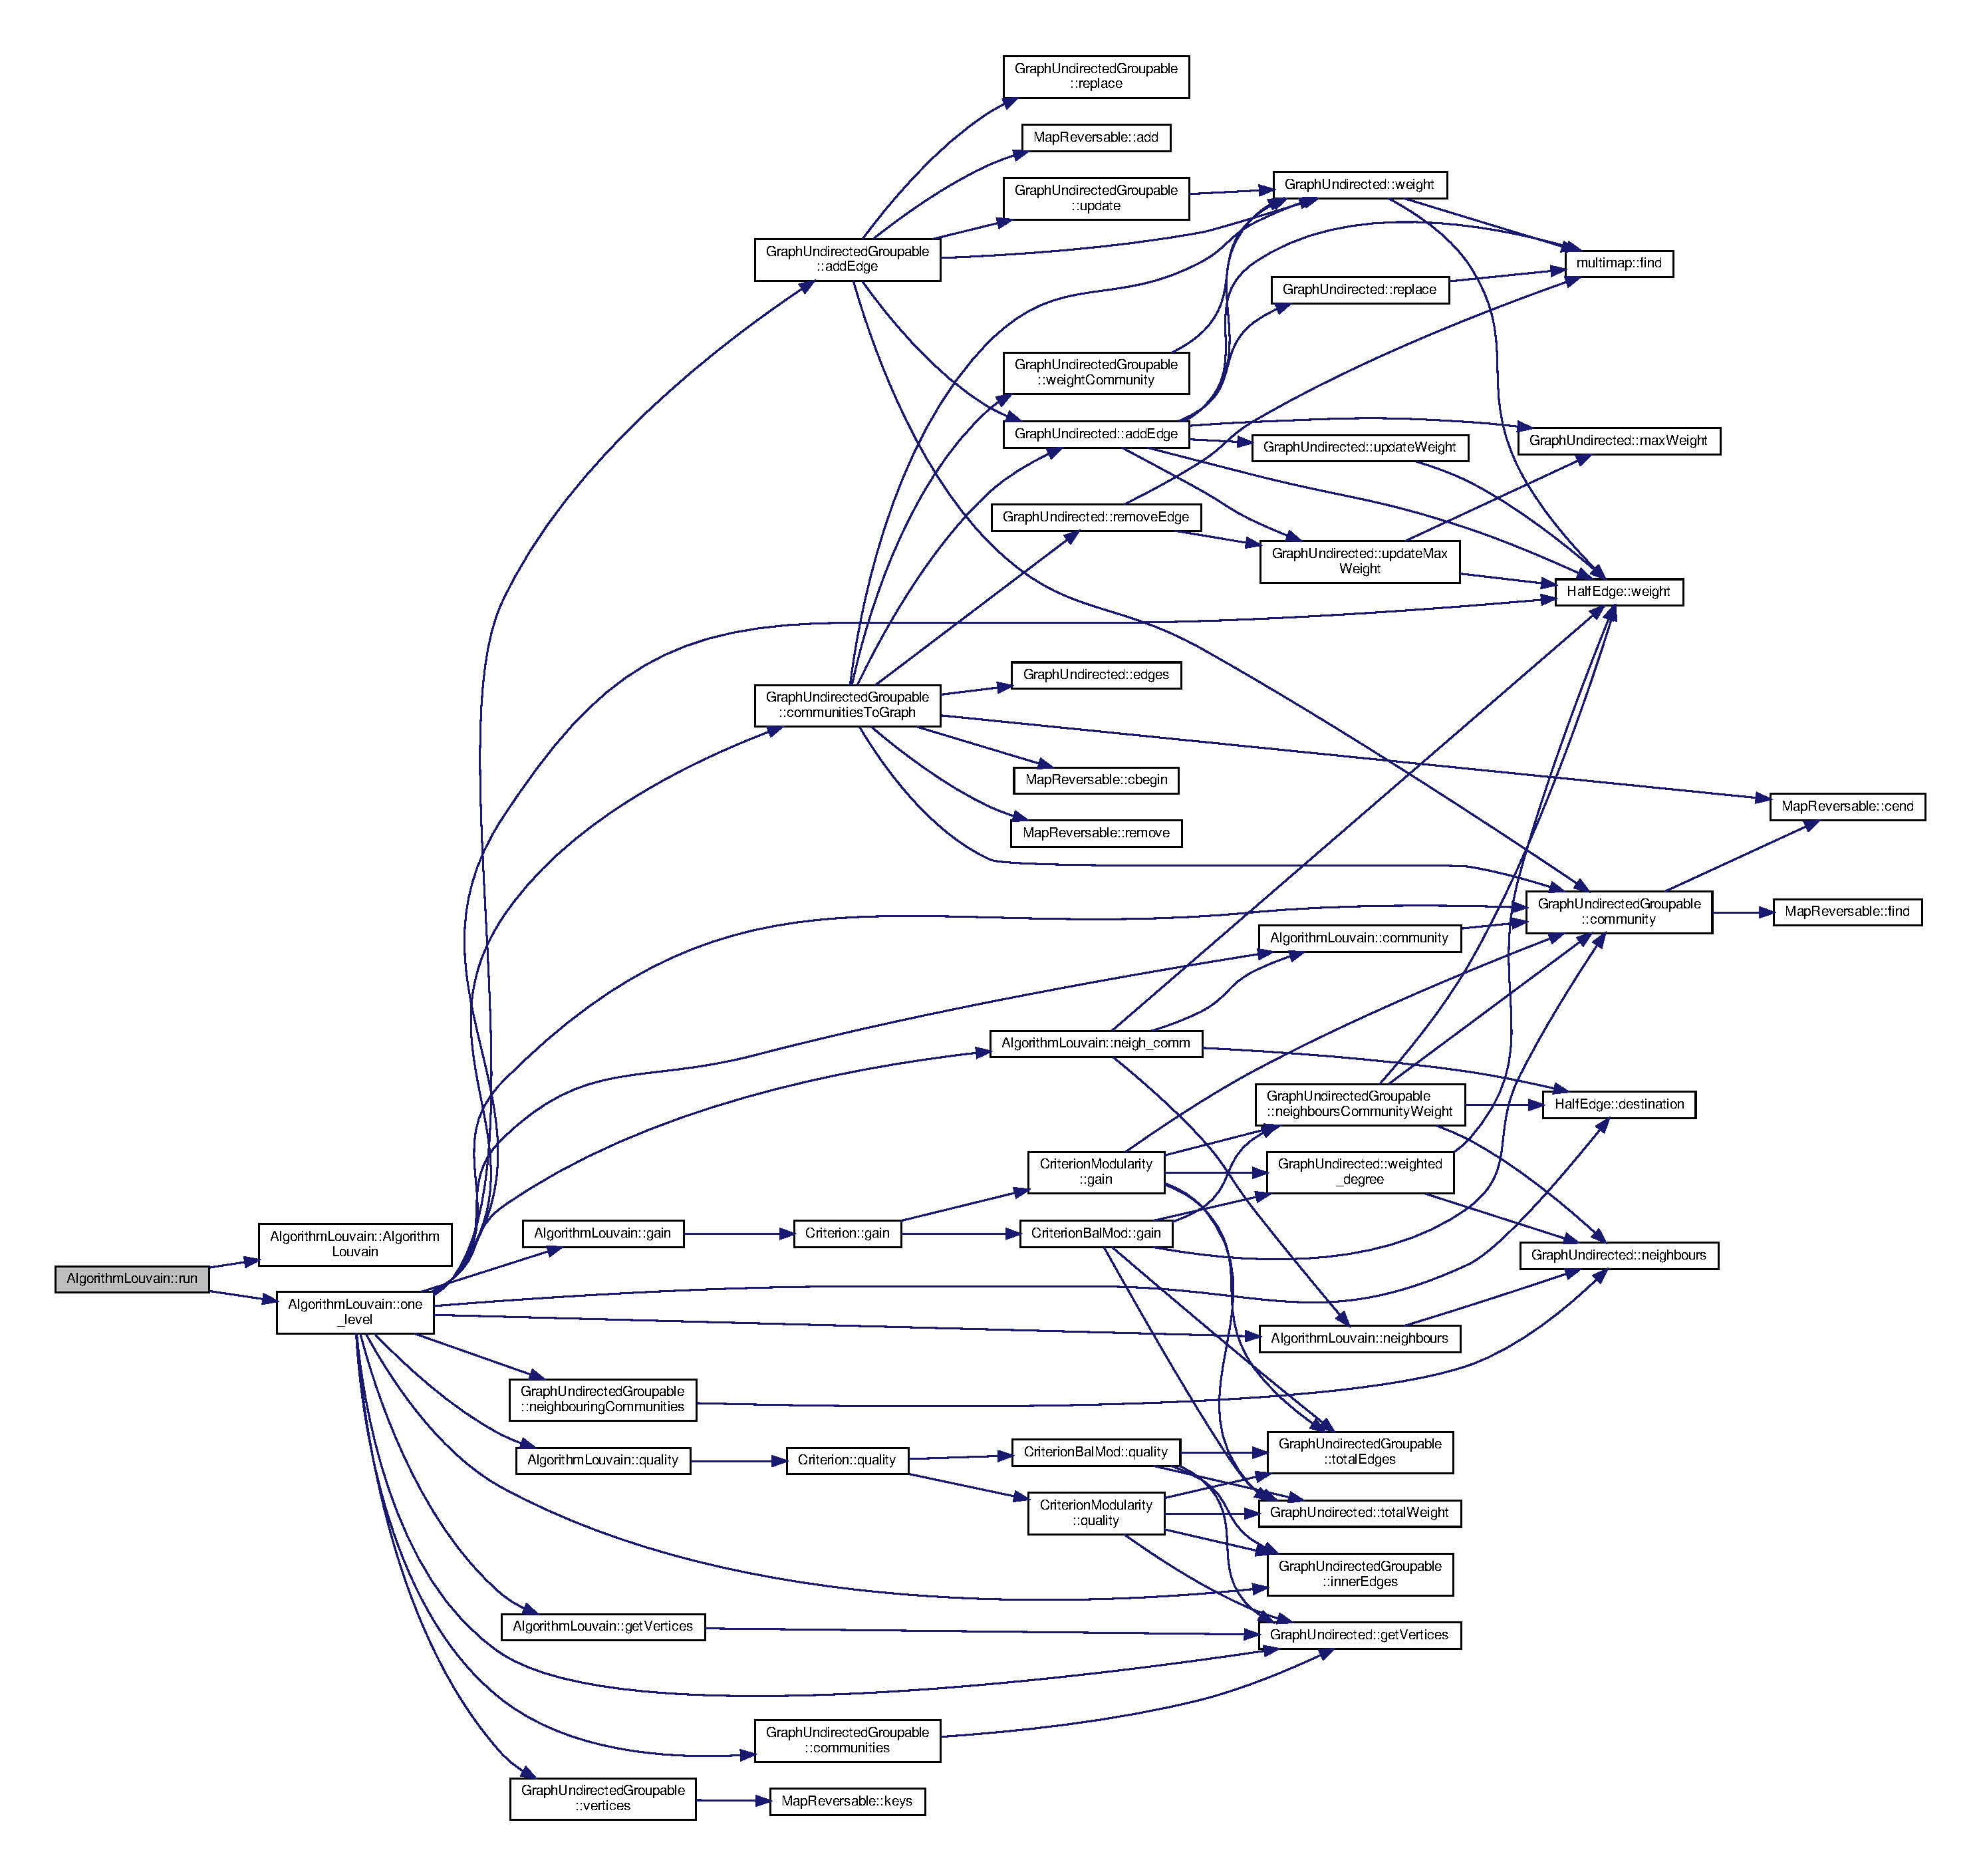
\includegraphics[width=350pt]{classAlgorithmLouvain_a0a72b9dda25c69d19996dc7448924c13_cgraph}
\end{center}
\end{figure}
\mbox{\Hypertarget{classAlgorithmLouvain_a2df60c50eb63b783ba0e9e77226bebee}\label{classAlgorithmLouvain_a2df60c50eb63b783ba0e9e77226bebee}} 
\index{Algorithm\+Louvain@{Algorithm\+Louvain}!to\+String@{to\+String}}
\index{to\+String@{to\+String}!Algorithm\+Louvain@{Algorithm\+Louvain}}
\subsubsection{\texorpdfstring{to\+String()}{toString()}}
{\footnotesize\ttfamily const std\+::string Algorithm\+Louvain\+::to\+String (\begin{DoxyParamCaption}\item[{const \hyperlink{classStringFormatter}{String\+Formatter} \&}]{sf = {\ttfamily \hyperlink{stringFormatter_8h_abf1349c8e24162d0134072aff288f2a2}{default\+String\+Formatter}} }\end{DoxyParamCaption}) const\hspace{0.3cm}{\ttfamily [inline]}}

Function that converts this object to a string representation. Might be useful for debugging.


\begin{DoxyParams}{Parameters}
{\em sf} & is a String\+Formater object that facilitates formating \\
\hline
\end{DoxyParams}
\begin{DoxyReturn}{Returns}
the string representing this object 
\end{DoxyReturn}


Definition at line 523 of file algorithm\+Louvain.\+h.



References String\+Formatter\+::build(), String\+Formatter\+::header(), Algorithm\+Base\+::to\+String(), and Graph\+Undirected\+Groupable\+::to\+String().



Referenced by Algorithm\+::to\+String().

Here is the call graph for this function\+:
\nopagebreak
\begin{figure}[H]
\begin{center}
\leavevmode
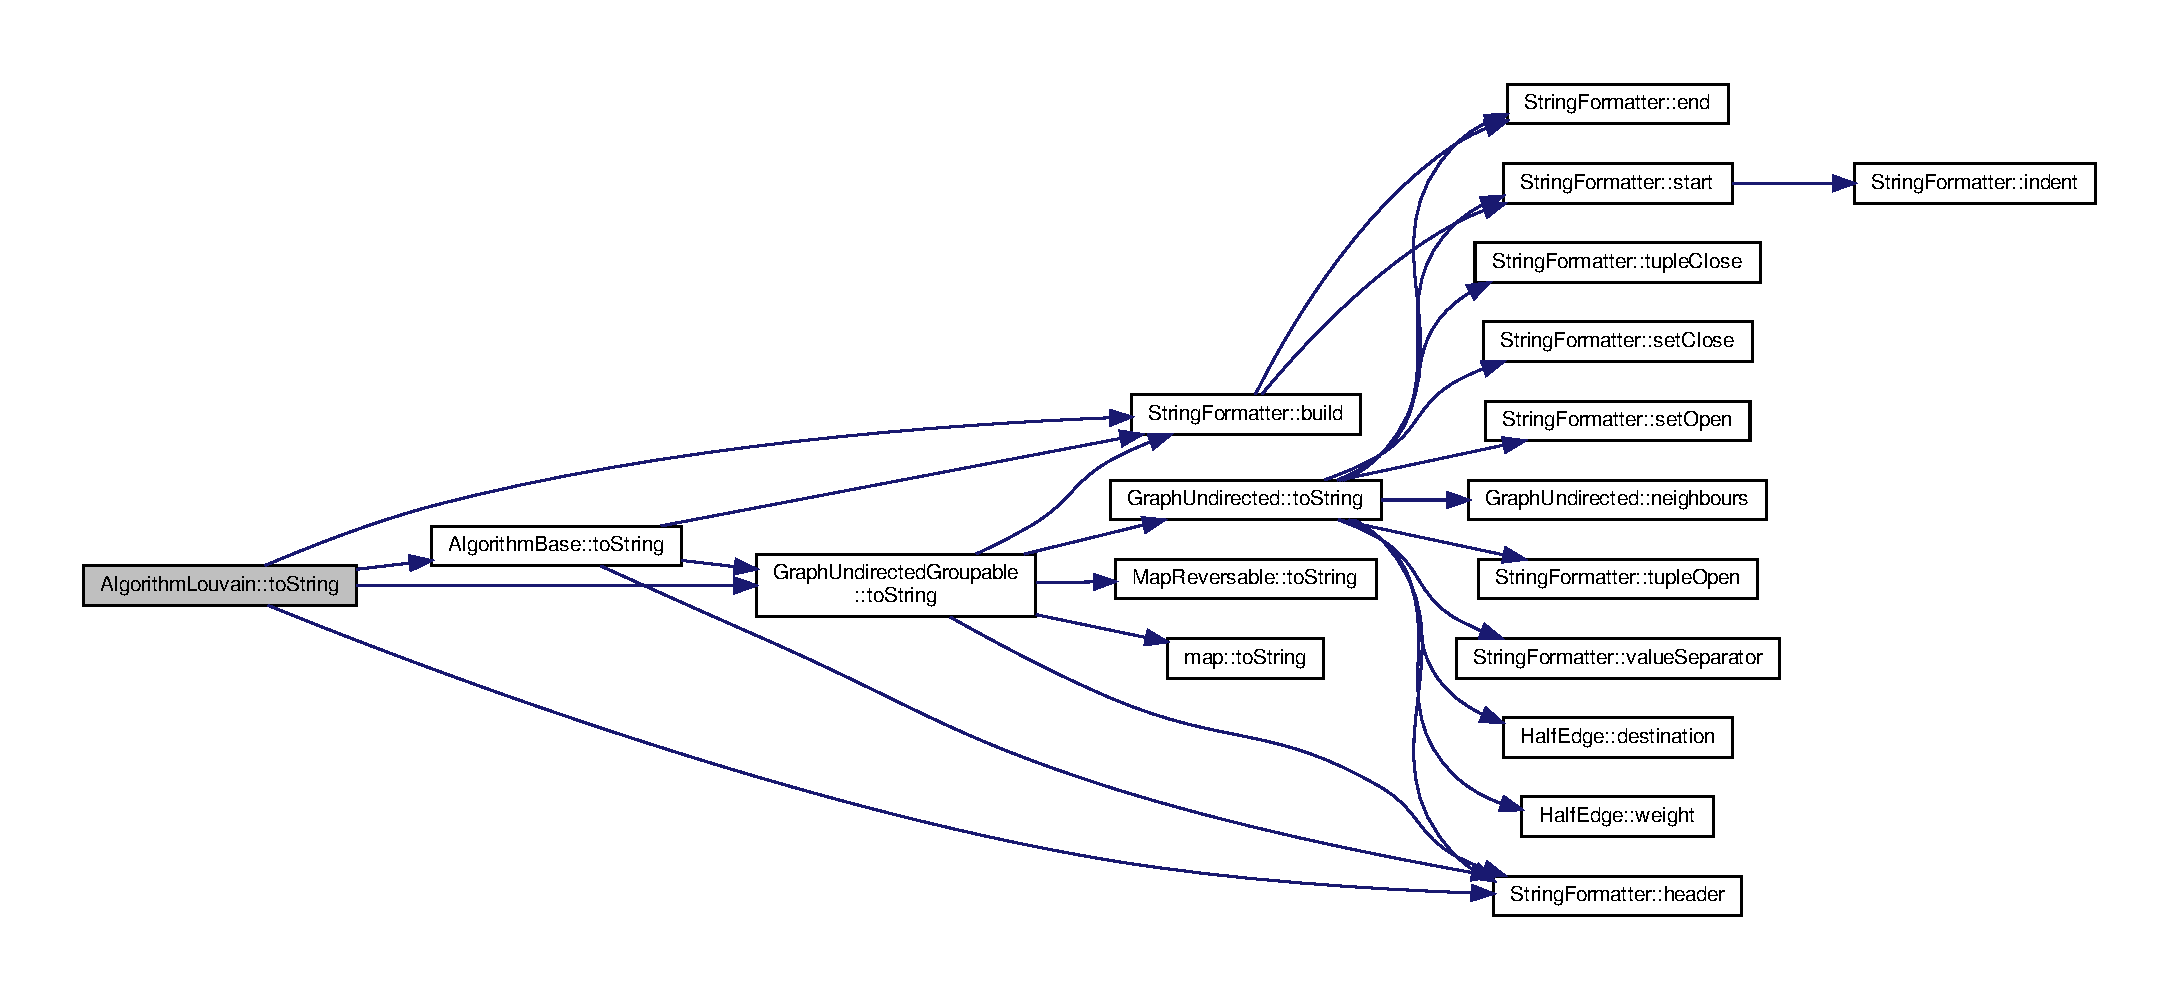
\includegraphics[width=350pt]{classAlgorithmLouvain_a2df60c50eb63b783ba0e9e77226bebee_cgraph}
\end{center}
\end{figure}
\mbox{\Hypertarget{classAlgorithmLouvain_a36a6536611d7c97d16f93245e2271867}\label{classAlgorithmLouvain_a36a6536611d7c97d16f93245e2271867}} 
\index{Algorithm\+Louvain@{Algorithm\+Louvain}!total\+Edges@{total\+Edges}}
\index{total\+Edges@{total\+Edges}!Algorithm\+Louvain@{Algorithm\+Louvain}}
\subsubsection{\texorpdfstring{total\+Edges()}{totalEdges()}}
{\footnotesize\ttfamily \hyperlink{edge_8h_a2e7ea3be891ac8b52f749ec73fee6dd2}{type\+Weight} Algorithm\+Louvain\+::total\+Edges (\begin{DoxyParamCaption}\item[{const \hyperlink{graphUndirectedGroupable_8h_a914da95c9ea7f14f4b7f875c36818556}{type\+Community} \&}]{c }\end{DoxyParamCaption}) const\hspace{0.3cm}{\ttfamily [inline]}, {\ttfamily [private]}}



Definition at line 87 of file algorithm\+Louvain.\+h.



References Algorithm\+Base\+::grph, and Graph\+Undirected\+Groupable\+::total\+Edges().

Here is the call graph for this function\+:
\nopagebreak
\begin{figure}[H]
\begin{center}
\leavevmode
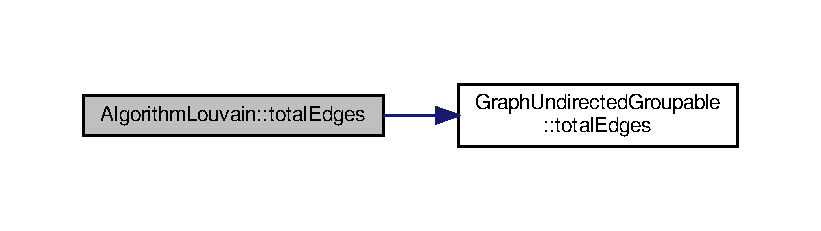
\includegraphics[width=350pt]{classAlgorithmLouvain_a36a6536611d7c97d16f93245e2271867_cgraph}
\end{center}
\end{figure}
\mbox{\Hypertarget{classAlgorithmLouvain_a6b38d3b1af94bb426b953473aa5647a4}\label{classAlgorithmLouvain_a6b38d3b1af94bb426b953473aa5647a4}} 
\index{Algorithm\+Louvain@{Algorithm\+Louvain}!total\+Weight@{total\+Weight}}
\index{total\+Weight@{total\+Weight}!Algorithm\+Louvain@{Algorithm\+Louvain}}
\subsubsection{\texorpdfstring{total\+Weight()}{totalWeight()}}
{\footnotesize\ttfamily const \hyperlink{edge_8h_a2e7ea3be891ac8b52f749ec73fee6dd2}{type\+Weight} Algorithm\+Louvain\+::total\+Weight (\begin{DoxyParamCaption}{ }\end{DoxyParamCaption}) const\hspace{0.3cm}{\ttfamily [inline]}, {\ttfamily [private]}}



Definition at line 137 of file algorithm\+Louvain.\+h.



References Algorithm\+Base\+::grph, and Graph\+Undirected\+::total\+Weight().

Here is the call graph for this function\+:
\nopagebreak
\begin{figure}[H]
\begin{center}
\leavevmode
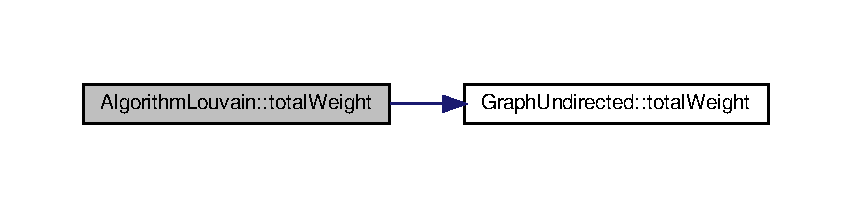
\includegraphics[width=350pt]{classAlgorithmLouvain_a6b38d3b1af94bb426b953473aa5647a4_cgraph}
\end{center}
\end{figure}
\mbox{\Hypertarget{classAlgorithmLouvain_a24c9f6d44d422eee2307c55540a8273c}\label{classAlgorithmLouvain_a24c9f6d44d422eee2307c55540a8273c}} 
\index{Algorithm\+Louvain@{Algorithm\+Louvain}!vertices@{vertices}}
\index{vertices@{vertices}!Algorithm\+Louvain@{Algorithm\+Louvain}}
\subsubsection{\texorpdfstring{vertices()}{vertices()}}
{\footnotesize\ttfamily \hyperlink{graphUndirectedGroupable_8h_ad440de7f8b59665f0705cc6f745aab09}{type\+Community\+List\+Range} Algorithm\+Louvain\+::vertices (\begin{DoxyParamCaption}\item[{const \hyperlink{graphUndirectedGroupable_8h_a914da95c9ea7f14f4b7f875c36818556}{type\+Community} \&}]{c }\end{DoxyParamCaption})\hspace{0.3cm}{\ttfamily [inline]}, {\ttfamily [private]}}



Definition at line 102 of file algorithm\+Louvain.\+h.



References Algorithm\+Base\+::grph, and Graph\+Undirected\+Groupable\+::vertices().

Here is the call graph for this function\+:
\nopagebreak
\begin{figure}[H]
\begin{center}
\leavevmode
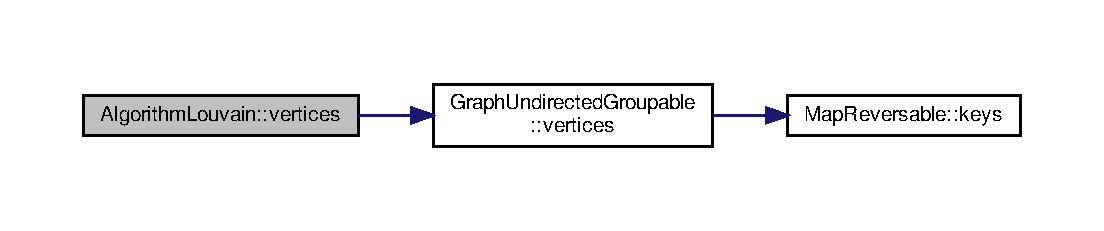
\includegraphics[width=350pt]{classAlgorithmLouvain_a24c9f6d44d422eee2307c55540a8273c_cgraph}
\end{center}
\end{figure}
\mbox{\Hypertarget{classAlgorithmLouvain_ab132e4f38f353713dc8c0c89b3bde576}\label{classAlgorithmLouvain_ab132e4f38f353713dc8c0c89b3bde576}} 
\index{Algorithm\+Louvain@{Algorithm\+Louvain}!vertices\+Count@{vertices\+Count}}
\index{vertices\+Count@{vertices\+Count}!Algorithm\+Louvain@{Algorithm\+Louvain}}
\subsubsection{\texorpdfstring{vertices\+Count()}{verticesCount()}}
{\footnotesize\ttfamily const \hyperlink{edge_8h_a2e7ea3be891ac8b52f749ec73fee6dd2}{type\+Weight} Algorithm\+Louvain\+::vertices\+Count (\begin{DoxyParamCaption}{ }\end{DoxyParamCaption}) const\hspace{0.3cm}{\ttfamily [inline]}, {\ttfamily [private]}}



Definition at line 142 of file algorithm\+Louvain.\+h.



References Algorithm\+Base\+::grph, and Graph\+Undirected\+::vertex\+Count().

Here is the call graph for this function\+:
\nopagebreak
\begin{figure}[H]
\begin{center}
\leavevmode
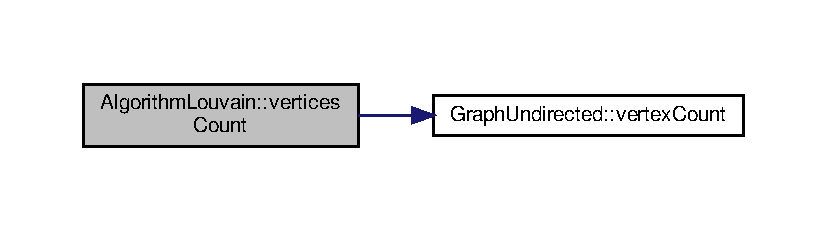
\includegraphics[width=350pt]{classAlgorithmLouvain_ab132e4f38f353713dc8c0c89b3bde576_cgraph}
\end{center}
\end{figure}
\mbox{\Hypertarget{classAlgorithmLouvain_a75a05ca235819217d3a91c1bd45def43}\label{classAlgorithmLouvain_a75a05ca235819217d3a91c1bd45def43}} 
\index{Algorithm\+Louvain@{Algorithm\+Louvain}!weighted\+\_\+degree@{weighted\+\_\+degree}}
\index{weighted\+\_\+degree@{weighted\+\_\+degree}!Algorithm\+Louvain@{Algorithm\+Louvain}}
\subsubsection{\texorpdfstring{weighted\+\_\+degree()}{weighted\_degree()}}
{\footnotesize\ttfamily \hyperlink{edge_8h_a2e7ea3be891ac8b52f749ec73fee6dd2}{type\+Weight} Algorithm\+Louvain\+::weighted\+\_\+degree (\begin{DoxyParamCaption}\item[{const \hyperlink{edge_8h_a5fbd20c46956d479cb10afc9855223f6}{type\+Vertex} \&}]{vertex }\end{DoxyParamCaption}) const\hspace{0.3cm}{\ttfamily [inline]}, {\ttfamily [private]}}



Definition at line 157 of file algorithm\+Louvain.\+h.



References Algorithm\+Base\+::grph, and Graph\+Undirected\+::weighted\+\_\+degree().

Here is the call graph for this function\+:
\nopagebreak
\begin{figure}[H]
\begin{center}
\leavevmode
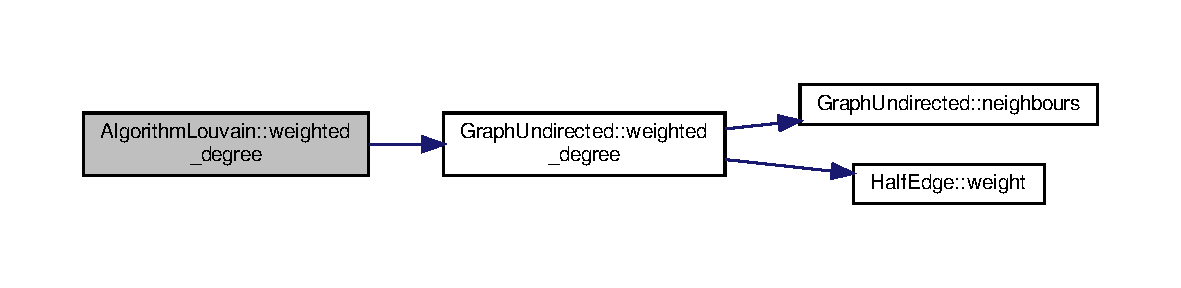
\includegraphics[width=350pt]{classAlgorithmLouvain_a75a05ca235819217d3a91c1bd45def43_cgraph}
\end{center}
\end{figure}


\subsection{Member Data Documentation}
\mbox{\Hypertarget{classAlgorithmLouvain_aa98d18e2734216898993b4269f84ac7b}\label{classAlgorithmLouvain_aa98d18e2734216898993b4269f84ac7b}} 
\index{Algorithm\+Louvain@{Algorithm\+Louvain}!cg@{cg}}
\index{cg@{cg}!Algorithm\+Louvain@{Algorithm\+Louvain}}
\subsubsection{\texorpdfstring{cg}{cg}}
{\footnotesize\ttfamily \hyperlink{classGraphUndirectedGroupable}{Graph\+Undirected\+Groupable} Algorithm\+Louvain\+::cg\hspace{0.3cm}{\ttfamily [private]}}



Definition at line 40 of file algorithm\+Louvain.\+h.

\mbox{\Hypertarget{classAlgorithmLouvain_a193c2370556007f36b44e03e2df47c2f}\label{classAlgorithmLouvain_a193c2370556007f36b44e03e2df47c2f}} 
\index{Algorithm\+Louvain@{Algorithm\+Louvain}!first\+Run@{first\+Run}}
\index{first\+Run@{first\+Run}!Algorithm\+Louvain@{Algorithm\+Louvain}}
\subsubsection{\texorpdfstring{first\+Run}{firstRun}}
{\footnotesize\ttfamily bool Algorithm\+Louvain\+::first\+Run =true\hspace{0.3cm}{\ttfamily [private]}}



Definition at line 56 of file algorithm\+Louvain.\+h.

\mbox{\Hypertarget{classAlgorithmLouvain_ab3b6b2b7f256ca9962d685d6507fad90}\label{classAlgorithmLouvain_ab3b6b2b7f256ca9962d685d6507fad90}} 
\index{Algorithm\+Louvain@{Algorithm\+Louvain}!qltc@{qltc}}
\index{qltc@{qltc}!Algorithm\+Louvain@{Algorithm\+Louvain}}
\subsubsection{\texorpdfstring{qltc}{qltc}}
{\footnotesize\ttfamily \hyperlink{classCriterion}{Criterion} Algorithm\+Louvain\+::qltc\hspace{0.3cm}{\ttfamily [private]}}



Definition at line 48 of file algorithm\+Louvain.\+h.



The documentation for this class was generated from the following file\+:\begin{DoxyCompactItemize}
\item 
R-\/\+C\+R\+A\+N/src/base/\+Cpp/\hyperlink{algorithmLouvain_8h}{algorithm\+Louvain.\+h}\end{DoxyCompactItemize}

\hypertarget{classCriterion}{}\section{Criterion Class Reference}
\label{classCriterion}\index{Criterion@{Criterion}}


Aggregator class for all criterion.  




{\ttfamily \#include $<$criterion.\+h$>$}



Inheritance diagram for Criterion\+:
\nopagebreak
\begin{figure}[H]
\begin{center}
\leavevmode
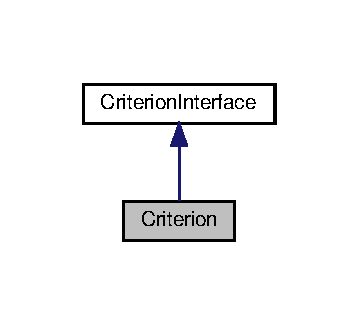
\includegraphics[width=172pt]{classCriterion__inherit__graph}
\end{center}
\end{figure}


Collaboration diagram for Criterion\+:
\nopagebreak
\begin{figure}[H]
\begin{center}
\leavevmode
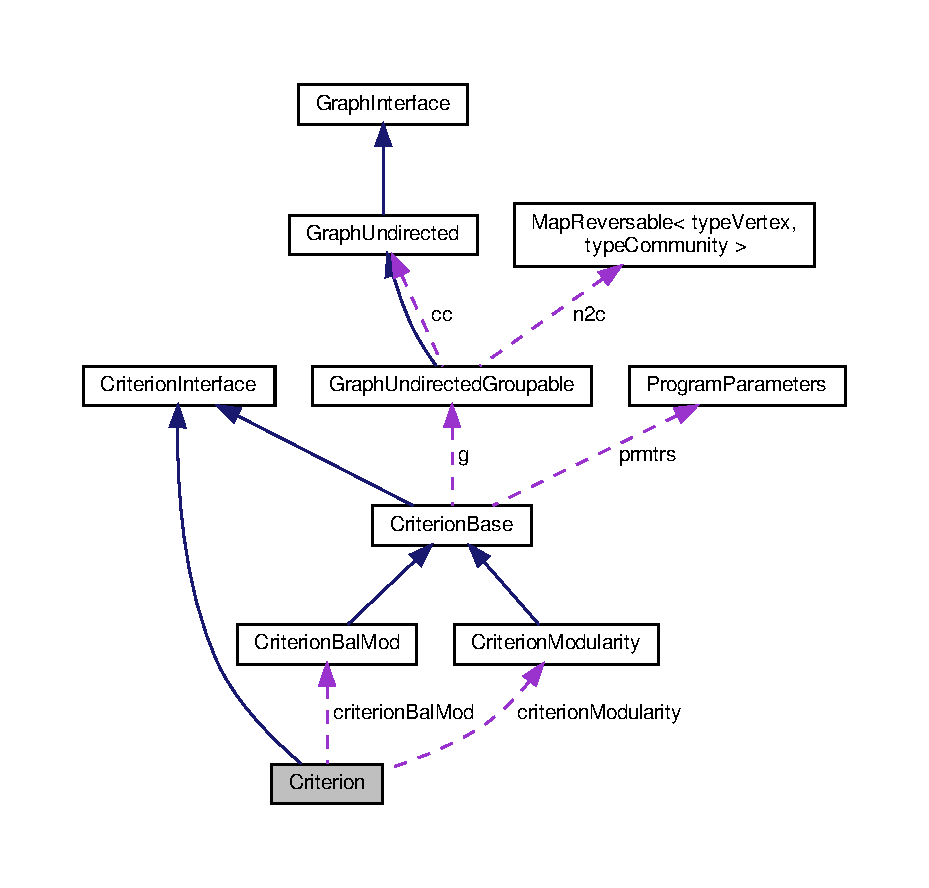
\includegraphics[width=350pt]{classCriterion__coll__graph}
\end{center}
\end{figure}
\subsection*{Public Types}
\begin{DoxyCompactItemize}
\item 
enum \hyperlink{classCriterion_a55594c223ce0837b8319c46c66cb648f}{C\+R\+I\+T\+E\+R\+I\+ON} \+: unsigned int \{ \hyperlink{classCriterion_a55594c223ce0837b8319c46c66cb648fa2a7d416fbe43baf234420601ea73d946}{C\+R\+I\+T\+E\+R\+I\+O\+N\+::\+M\+O\+D\+U\+L\+A\+R\+I\+TY} =1, 
\hyperlink{classCriterion_a55594c223ce0837b8319c46c66cb648fa2ca6c7acaa036f0d3b18d83b688b2df9}{C\+R\+I\+T\+E\+R\+I\+O\+N\+::\+B\+A\+L\+M\+OD}
 \}
\end{DoxyCompactItemize}
\subsection*{Public Member Functions}
\begin{DoxyCompactItemize}
\item 
\hyperlink{classCriterion_ac880ed791be9ad5cf41fe8561bdec35f}{Criterion} (const \hyperlink{classGraphUndirectedGroupable}{Graph\+Undirected\+Groupable} \&graph, const \hyperlink{classCriterion_a55594c223ce0837b8319c46c66cb648f}{C\+R\+I\+T\+E\+R\+I\+ON} \&criterion, const \hyperlink{structProgramParameters}{Program\+Parameters} \&parameters=\hyperlink{program_8h_ae2d819404495f80f31db7676c1329d19}{arguments\+Default})
\item 
\hyperlink{classCriterion_ae66e2b8131ae4a5e7945d9fdc1b2dcc2}{$\sim$\+Criterion} ()
\item 
\hyperlink{criterionInterface_8h_af71ff22f6355fd69a4a62104bfd59a83}{type\+Criterion} \hyperlink{classCriterion_a99e23ddc517ca3f2ea4766a5b4be0e3e}{gain} (const \hyperlink{edge_8h_a5fbd20c46956d479cb10afc9855223f6}{type\+Vertex} \&vertex, const \hyperlink{graphUndirectedGroupable_8h_a914da95c9ea7f14f4b7f875c36818556}{type\+Community} \&comm) const
\item 
\hyperlink{criterionInterface_8h_af71ff22f6355fd69a4a62104bfd59a83}{type\+Criterion} \hyperlink{classCriterion_a1f8b3a7bf56b5434b04d5366d754d459}{quality} () const
\item 
\hyperlink{classCriterion_a55594c223ce0837b8319c46c66cb648f}{C\+R\+I\+T\+E\+R\+I\+ON} \hyperlink{classCriterion_a023f88034d2712af46160f1842388b0d}{type} () const
\end{DoxyCompactItemize}
\subsection*{Private Attributes}
\begin{DoxyCompactItemize}
\item 
const \hyperlink{classCriterion_a55594c223ce0837b8319c46c66cb648f}{C\+R\+I\+T\+E\+R\+I\+ON} \hyperlink{classCriterion_af38092427520b56e2301f14e7fc71dbb}{crtrn}
\item 
\hyperlink{classCriterionModularity}{Criterion\+Modularity} \hyperlink{classCriterion_ae3432ace13d3191c7f6f33c833eb3b82}{criterion\+Modularity}
\item 
\hyperlink{classCriterionBalMod}{Criterion\+Bal\+Mod} \hyperlink{classCriterion_a164dd99a6707997bb916a1516e1cd327}{criterion\+Bal\+Mod}
\end{DoxyCompactItemize}


\subsection{Detailed Description}
Aggregator class for all criterion. 

It is a simple class that only instantiates all criterion and dispatches function calls to the correct one.

\begin{DoxyAuthor}{Author}
poltergeist0
\end{DoxyAuthor}
\begin{DoxyDate}{Date}
2018-\/08-\/19 
\end{DoxyDate}


Definition at line 46 of file criterion.\+h.



\subsection{Member Enumeration Documentation}
\mbox{\Hypertarget{classCriterion_a55594c223ce0837b8319c46c66cb648f}\label{classCriterion_a55594c223ce0837b8319c46c66cb648f}} 
\index{Criterion@{Criterion}!C\+R\+I\+T\+E\+R\+I\+ON@{C\+R\+I\+T\+E\+R\+I\+ON}}
\index{C\+R\+I\+T\+E\+R\+I\+ON@{C\+R\+I\+T\+E\+R\+I\+ON}!Criterion@{Criterion}}
\subsubsection{\texorpdfstring{C\+R\+I\+T\+E\+R\+I\+ON}{CRITERION}}
{\footnotesize\ttfamily enum \hyperlink{classCriterion_a55594c223ce0837b8319c46c66cb648f}{Criterion\+::\+C\+R\+I\+T\+E\+R\+I\+ON} \+: unsigned int\hspace{0.3cm}{\ttfamily [strong]}}

Enumeration with the list of supported criterion for algorithms implemented in C++. This enumeration must start at 1 since this code is used in R and R indexing (for arrays, etc) starts at 1 instead of 0. Otherwise C++ would assign the first criterion a 0. \begin{DoxyEnumFields}{Enumerator}
\raisebox{\heightof{T}}[0pt][0pt]{\index{M\+O\+D\+U\+L\+A\+R\+I\+TY@{M\+O\+D\+U\+L\+A\+R\+I\+TY}!Criterion@{Criterion}}\index{Criterion@{Criterion}!M\+O\+D\+U\+L\+A\+R\+I\+TY@{M\+O\+D\+U\+L\+A\+R\+I\+TY}}}\mbox{\Hypertarget{classCriterion_a55594c223ce0837b8319c46c66cb648fa2a7d416fbe43baf234420601ea73d946}\label{classCriterion_a55594c223ce0837b8319c46c66cb648fa2a7d416fbe43baf234420601ea73d946}} 
M\+O\+D\+U\+L\+A\+R\+I\+TY&\\
\hline

\raisebox{\heightof{T}}[0pt][0pt]{\index{B\+A\+L\+M\+OD@{B\+A\+L\+M\+OD}!Criterion@{Criterion}}\index{Criterion@{Criterion}!B\+A\+L\+M\+OD@{B\+A\+L\+M\+OD}}}\mbox{\Hypertarget{classCriterion_a55594c223ce0837b8319c46c66cb648fa2ca6c7acaa036f0d3b18d83b688b2df9}\label{classCriterion_a55594c223ce0837b8319c46c66cb648fa2ca6c7acaa036f0d3b18d83b688b2df9}} 
B\+A\+L\+M\+OD&\\
\hline

\end{DoxyEnumFields}


Definition at line 60 of file criterion.\+h.



\subsection{Constructor \& Destructor Documentation}
\mbox{\Hypertarget{classCriterion_ac880ed791be9ad5cf41fe8561bdec35f}\label{classCriterion_ac880ed791be9ad5cf41fe8561bdec35f}} 
\index{Criterion@{Criterion}!Criterion@{Criterion}}
\index{Criterion@{Criterion}!Criterion@{Criterion}}
\subsubsection{\texorpdfstring{Criterion()}{Criterion()}}
{\footnotesize\ttfamily Criterion\+::\+Criterion (\begin{DoxyParamCaption}\item[{const \hyperlink{classGraphUndirectedGroupable}{Graph\+Undirected\+Groupable} \&}]{graph,  }\item[{const \hyperlink{classCriterion_a55594c223ce0837b8319c46c66cb648f}{C\+R\+I\+T\+E\+R\+I\+ON} \&}]{criterion,  }\item[{const \hyperlink{structProgramParameters}{Program\+Parameters} \&}]{parameters = {\ttfamily \hyperlink{program_8h_ae2d819404495f80f31db7676c1329d19}{arguments\+Default}} }\end{DoxyParamCaption})\hspace{0.3cm}{\ttfamily [inline]}}

Constructor


\begin{DoxyParams}{Parameters}
{\em graph} & \\
\hline
{\em criterion} & \\
\hline
{\em parameters} & \\
\hline
\end{DoxyParams}


Definition at line 90 of file criterion.\+h.

\mbox{\Hypertarget{classCriterion_ae66e2b8131ae4a5e7945d9fdc1b2dcc2}\label{classCriterion_ae66e2b8131ae4a5e7945d9fdc1b2dcc2}} 
\index{Criterion@{Criterion}!````~Criterion@{$\sim$\+Criterion}}
\index{````~Criterion@{$\sim$\+Criterion}!Criterion@{Criterion}}
\subsubsection{\texorpdfstring{$\sim$\+Criterion()}{~Criterion()}}
{\footnotesize\ttfamily Criterion\+::$\sim$\+Criterion (\begin{DoxyParamCaption}{ }\end{DoxyParamCaption})\hspace{0.3cm}{\ttfamily [inline]}}

Destructor 

Definition at line 108 of file criterion.\+h.



\subsection{Member Function Documentation}
\mbox{\Hypertarget{classCriterion_a99e23ddc517ca3f2ea4766a5b4be0e3e}\label{classCriterion_a99e23ddc517ca3f2ea4766a5b4be0e3e}} 
\index{Criterion@{Criterion}!gain@{gain}}
\index{gain@{gain}!Criterion@{Criterion}}
\subsubsection{\texorpdfstring{gain()}{gain()}}
{\footnotesize\ttfamily \hyperlink{criterionInterface_8h_af71ff22f6355fd69a4a62104bfd59a83}{type\+Criterion} Criterion\+::gain (\begin{DoxyParamCaption}\item[{const \hyperlink{edge_8h_a5fbd20c46956d479cb10afc9855223f6}{type\+Vertex} \&}]{vertex,  }\item[{const \hyperlink{graphUndirectedGroupable_8h_a914da95c9ea7f14f4b7f875c36818556}{type\+Community} \&}]{comm }\end{DoxyParamCaption}) const\hspace{0.3cm}{\ttfamily [inline]}, {\ttfamily [virtual]}}

compute the quality obtained if the given vertex was moved from its current community to the given community


\begin{DoxyParams}{Parameters}
{\em vertex} & \\
\hline
{\em comm} & new potential community for given vertex \\
\hline
\end{DoxyParams}
\begin{DoxyReturn}{Returns}
the quality, which may be positive or negative 
\end{DoxyReturn}


Implements \hyperlink{classCriterionInterface_aa0beec8287cd70e16c057e7995d0caca}{Criterion\+Interface}.



Definition at line 118 of file criterion.\+h.



References B\+A\+L\+M\+OD, Criterion\+Bal\+Mod\+::gain(), Criterion\+Modularity\+::gain(), and M\+O\+D\+U\+L\+A\+R\+I\+TY.



Referenced by Algorithm\+Louvain\+::gain().

Here is the call graph for this function\+:
\nopagebreak
\begin{figure}[H]
\begin{center}
\leavevmode
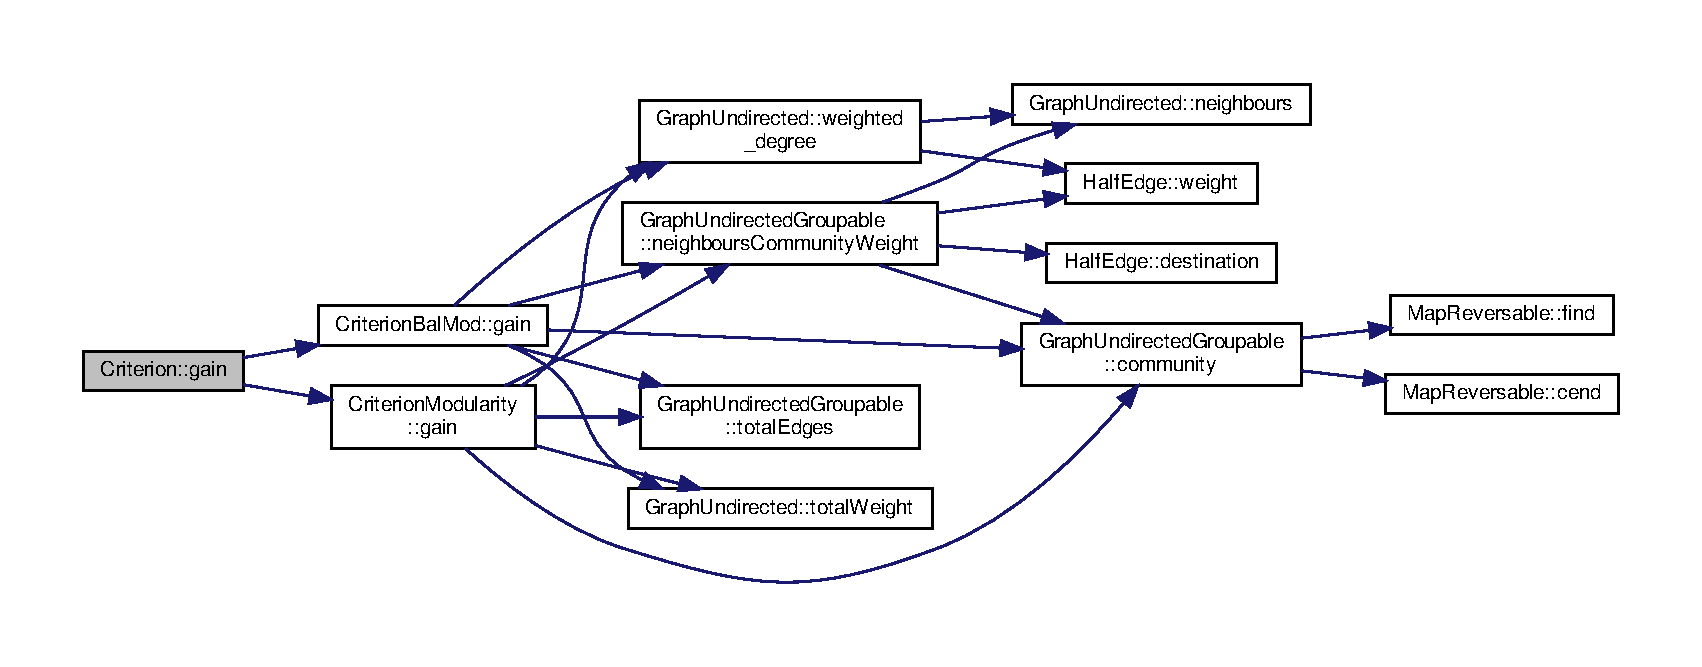
\includegraphics[width=350pt]{classCriterion_a99e23ddc517ca3f2ea4766a5b4be0e3e_cgraph}
\end{center}
\end{figure}
\mbox{\Hypertarget{classCriterion_a1f8b3a7bf56b5434b04d5366d754d459}\label{classCriterion_a1f8b3a7bf56b5434b04d5366d754d459}} 
\index{Criterion@{Criterion}!quality@{quality}}
\index{quality@{quality}!Criterion@{Criterion}}
\subsubsection{\texorpdfstring{quality()}{quality()}}
{\footnotesize\ttfamily \hyperlink{criterionInterface_8h_af71ff22f6355fd69a4a62104bfd59a83}{type\+Criterion} Criterion\+::quality (\begin{DoxyParamCaption}{ }\end{DoxyParamCaption}) const\hspace{0.3cm}{\ttfamily [inline]}, {\ttfamily [virtual]}}

compute the quality of the current partition scheme

\begin{DoxyReturn}{Returns}
the quality value 
\end{DoxyReturn}


Implements \hyperlink{classCriterionInterface_a5d287dc7755f7ce7d6a3d91f0d8fa5de}{Criterion\+Interface}.



Definition at line 136 of file criterion.\+h.



References B\+A\+L\+M\+OD, M\+O\+D\+U\+L\+A\+R\+I\+TY, Criterion\+Bal\+Mod\+::quality(), and Criterion\+Modularity\+::quality().



Referenced by Dyn\+Comm\+Base\+::quality(), and Algorithm\+Louvain\+::quality().

Here is the call graph for this function\+:
\nopagebreak
\begin{figure}[H]
\begin{center}
\leavevmode
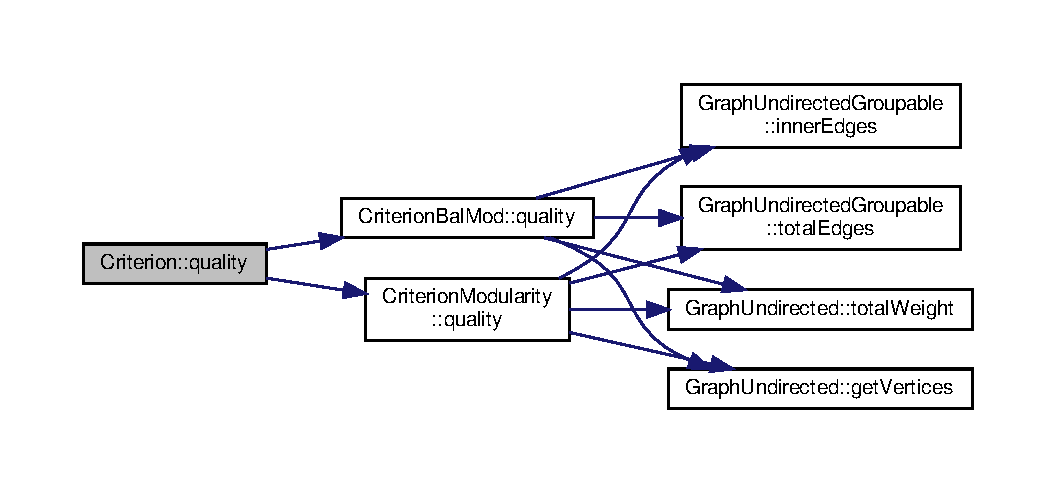
\includegraphics[width=350pt]{classCriterion_a1f8b3a7bf56b5434b04d5366d754d459_cgraph}
\end{center}
\end{figure}
\mbox{\Hypertarget{classCriterion_a023f88034d2712af46160f1842388b0d}\label{classCriterion_a023f88034d2712af46160f1842388b0d}} 
\index{Criterion@{Criterion}!type@{type}}
\index{type@{type}!Criterion@{Criterion}}
\subsubsection{\texorpdfstring{type()}{type()}}
{\footnotesize\ttfamily \hyperlink{classCriterion_a55594c223ce0837b8319c46c66cb648f}{C\+R\+I\+T\+E\+R\+I\+ON} Criterion\+::type (\begin{DoxyParamCaption}{ }\end{DoxyParamCaption}) const\hspace{0.3cm}{\ttfamily [inline]}}

\begin{DoxyReturn}{Returns}
the chosen criterion 
\end{DoxyReturn}


Definition at line 153 of file criterion.\+h.



References crtrn.



\subsection{Member Data Documentation}
\mbox{\Hypertarget{classCriterion_a164dd99a6707997bb916a1516e1cd327}\label{classCriterion_a164dd99a6707997bb916a1516e1cd327}} 
\index{Criterion@{Criterion}!criterion\+Bal\+Mod@{criterion\+Bal\+Mod}}
\index{criterion\+Bal\+Mod@{criterion\+Bal\+Mod}!Criterion@{Criterion}}
\subsubsection{\texorpdfstring{criterion\+Bal\+Mod}{criterionBalMod}}
{\footnotesize\ttfamily \hyperlink{classCriterionBalMod}{Criterion\+Bal\+Mod} Criterion\+::criterion\+Bal\+Mod\hspace{0.3cm}{\ttfamily [private]}}



Definition at line 73 of file criterion.\+h.

\mbox{\Hypertarget{classCriterion_ae3432ace13d3191c7f6f33c833eb3b82}\label{classCriterion_ae3432ace13d3191c7f6f33c833eb3b82}} 
\index{Criterion@{Criterion}!criterion\+Modularity@{criterion\+Modularity}}
\index{criterion\+Modularity@{criterion\+Modularity}!Criterion@{Criterion}}
\subsubsection{\texorpdfstring{criterion\+Modularity}{criterionModularity}}
{\footnotesize\ttfamily \hyperlink{classCriterionModularity}{Criterion\+Modularity} Criterion\+::criterion\+Modularity\hspace{0.3cm}{\ttfamily [private]}}



Definition at line 72 of file criterion.\+h.

\mbox{\Hypertarget{classCriterion_af38092427520b56e2301f14e7fc71dbb}\label{classCriterion_af38092427520b56e2301f14e7fc71dbb}} 
\index{Criterion@{Criterion}!crtrn@{crtrn}}
\index{crtrn@{crtrn}!Criterion@{Criterion}}
\subsubsection{\texorpdfstring{crtrn}{crtrn}}
{\footnotesize\ttfamily const \hyperlink{classCriterion_a55594c223ce0837b8319c46c66cb648f}{C\+R\+I\+T\+E\+R\+I\+ON} Criterion\+::crtrn\hspace{0.3cm}{\ttfamily [private]}}



Definition at line 67 of file criterion.\+h.



Referenced by type().



The documentation for this class was generated from the following file\+:\begin{DoxyCompactItemize}
\item 
R-\/\+C\+R\+A\+N/src/base/\+Cpp/\hyperlink{criterion_8h}{criterion.\+h}\end{DoxyCompactItemize}

\hypertarget{classCriterionBalMod}{}\section{Criterion\+Bal\+Mod Class Reference}
\label{classCriterionBalMod}\index{Criterion\+Bal\+Mod@{Criterion\+Bal\+Mod}}


Balanced Modularity criterion.  




{\ttfamily \#include $<$criterion\+Bal\+Mod.\+h$>$}



Inheritance diagram for Criterion\+Bal\+Mod\+:
\nopagebreak
\begin{figure}[H]
\begin{center}
\leavevmode
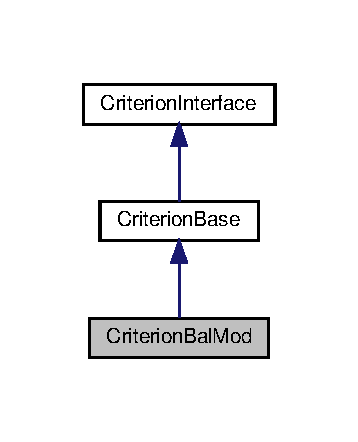
\includegraphics[width=172pt]{classCriterionBalMod__inherit__graph}
\end{center}
\end{figure}


Collaboration diagram for Criterion\+Bal\+Mod\+:
\nopagebreak
\begin{figure}[H]
\begin{center}
\leavevmode
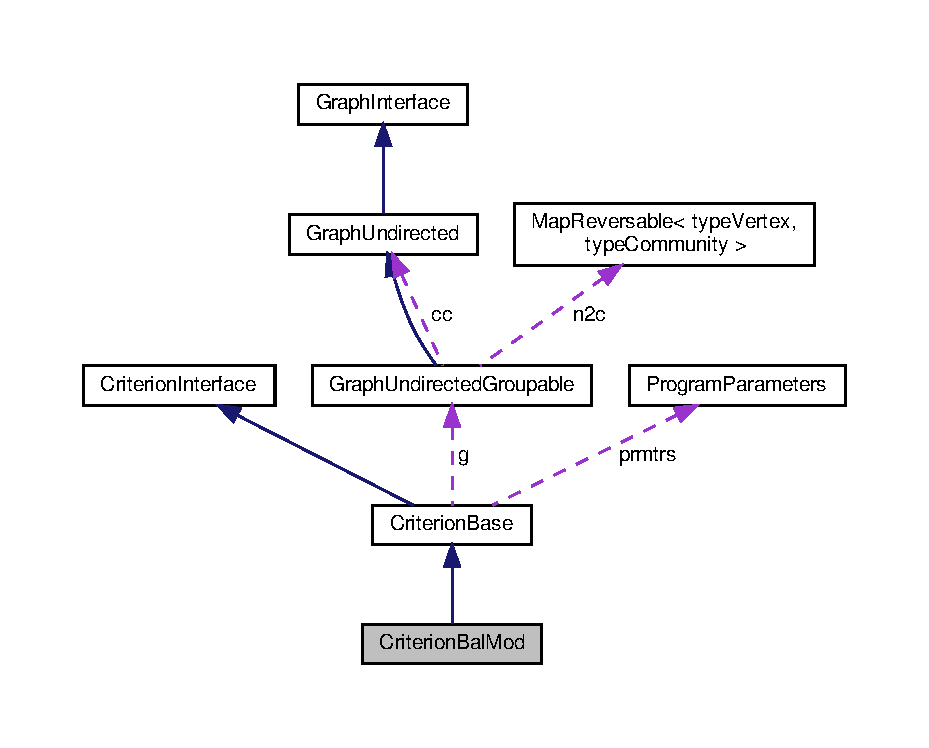
\includegraphics[width=350pt]{classCriterionBalMod__coll__graph}
\end{center}
\end{figure}
\subsection*{Public Member Functions}
\begin{DoxyCompactItemize}
\item 
\hyperlink{classCriterionBalMod_a2ac41e4b98142642daaeff16f87fd1b8}{Criterion\+Bal\+Mod} (const \hyperlink{classGraphUndirectedGroupable}{Graph\+Undirected\+Groupable} \&graph, const \hyperlink{structProgramParameters}{Program\+Parameters} \&parameters=\hyperlink{program_8h_ae2d819404495f80f31db7676c1329d19}{arguments\+Default})
\item 
\hyperlink{classCriterionBalMod_a7b436498c68a76ecd7adecc9280900d0}{$\sim$\+Criterion\+Bal\+Mod} ()
\item 
\hyperlink{criterionInterface_8h_af71ff22f6355fd69a4a62104bfd59a83}{type\+Criterion} \hyperlink{classCriterionBalMod_acf5001622eb8c495a5d5e8f044c22395}{gain} (const \hyperlink{edge_8h_a5fbd20c46956d479cb10afc9855223f6}{type\+Vertex} \&vertex, const \hyperlink{graphUndirectedGroupable_8h_a914da95c9ea7f14f4b7f875c36818556}{type\+Community} \&comm) const
\item 
\hyperlink{criterionInterface_8h_af71ff22f6355fd69a4a62104bfd59a83}{type\+Criterion} \hyperlink{classCriterionBalMod_a87c0ccb5e2a851420dc82bd23cc31716}{quality} () const
\end{DoxyCompactItemize}
\subsection*{Additional Inherited Members}


\subsection{Detailed Description}
Balanced Modularity criterion. 

\begin{DoxyAuthor}{Author}
poltergeist0
\end{DoxyAuthor}
\begin{DoxyDate}{Date}
2018-\/08-\/20 
\end{DoxyDate}


Definition at line 29 of file criterion\+Bal\+Mod.\+h.



\subsection{Constructor \& Destructor Documentation}
\mbox{\Hypertarget{classCriterionBalMod_a2ac41e4b98142642daaeff16f87fd1b8}\label{classCriterionBalMod_a2ac41e4b98142642daaeff16f87fd1b8}} 
\index{Criterion\+Bal\+Mod@{Criterion\+Bal\+Mod}!Criterion\+Bal\+Mod@{Criterion\+Bal\+Mod}}
\index{Criterion\+Bal\+Mod@{Criterion\+Bal\+Mod}!Criterion\+Bal\+Mod@{Criterion\+Bal\+Mod}}
\subsubsection{\texorpdfstring{Criterion\+Bal\+Mod()}{CriterionBalMod()}}
{\footnotesize\ttfamily Criterion\+Bal\+Mod\+::\+Criterion\+Bal\+Mod (\begin{DoxyParamCaption}\item[{const \hyperlink{classGraphUndirectedGroupable}{Graph\+Undirected\+Groupable} \&}]{graph,  }\item[{const \hyperlink{structProgramParameters}{Program\+Parameters} \&}]{parameters = {\ttfamily \hyperlink{program_8h_ae2d819404495f80f31db7676c1329d19}{arguments\+Default}} }\end{DoxyParamCaption})\hspace{0.3cm}{\ttfamily [inline]}}

Constructor.


\begin{DoxyParams}{Parameters}
{\em graph} & reference to the graph object \\
\hline
{\em parameters} & reference to the parameters object \\
\hline
\end{DoxyParams}


Definition at line 39 of file criterion\+Bal\+Mod.\+h.

\mbox{\Hypertarget{classCriterionBalMod_a7b436498c68a76ecd7adecc9280900d0}\label{classCriterionBalMod_a7b436498c68a76ecd7adecc9280900d0}} 
\index{Criterion\+Bal\+Mod@{Criterion\+Bal\+Mod}!````~Criterion\+Bal\+Mod@{$\sim$\+Criterion\+Bal\+Mod}}
\index{````~Criterion\+Bal\+Mod@{$\sim$\+Criterion\+Bal\+Mod}!Criterion\+Bal\+Mod@{Criterion\+Bal\+Mod}}
\subsubsection{\texorpdfstring{$\sim$\+Criterion\+Bal\+Mod()}{~CriterionBalMod()}}
{\footnotesize\ttfamily Criterion\+Bal\+Mod\+::$\sim$\+Criterion\+Bal\+Mod (\begin{DoxyParamCaption}{ }\end{DoxyParamCaption})\hspace{0.3cm}{\ttfamily [inline]}}

Destructor 

Definition at line 44 of file criterion\+Bal\+Mod.\+h.



\subsection{Member Function Documentation}
\mbox{\Hypertarget{classCriterionBalMod_acf5001622eb8c495a5d5e8f044c22395}\label{classCriterionBalMod_acf5001622eb8c495a5d5e8f044c22395}} 
\index{Criterion\+Bal\+Mod@{Criterion\+Bal\+Mod}!gain@{gain}}
\index{gain@{gain}!Criterion\+Bal\+Mod@{Criterion\+Bal\+Mod}}
\subsubsection{\texorpdfstring{gain()}{gain()}}
{\footnotesize\ttfamily \hyperlink{criterionInterface_8h_af71ff22f6355fd69a4a62104bfd59a83}{type\+Criterion} Criterion\+Bal\+Mod\+::gain (\begin{DoxyParamCaption}\item[{const \hyperlink{edge_8h_a5fbd20c46956d479cb10afc9855223f6}{type\+Vertex} \&}]{vertex,  }\item[{const \hyperlink{graphUndirectedGroupable_8h_a914da95c9ea7f14f4b7f875c36818556}{type\+Community} \&}]{comm }\end{DoxyParamCaption}) const\hspace{0.3cm}{\ttfamily [inline]}, {\ttfamily [virtual]}}

compute the quality obtained if the given vertex was moved from its current community to the given community


\begin{DoxyParams}{Parameters}
{\em vertex} & \\
\hline
{\em comm} & new potential community for given vertex \\
\hline
\end{DoxyParams}
\begin{DoxyReturn}{Returns}
the quality, which may be positive or negative 
\end{DoxyReturn}


Implements \hyperlink{classCriterionInterface_aa0beec8287cd70e16c057e7995d0caca}{Criterion\+Interface}.



Definition at line 54 of file criterion\+Bal\+Mod.\+h.



References Graph\+Undirected\+Groupable\+::community(), Criterion\+Base\+::g, Graph\+Undirected\+Groupable\+::neighbors\+Community\+Weight(), Graph\+Undirected\+Groupable\+::total\+Edges(), Graph\+Undirected\+::total\+Weight(), and Graph\+Undirected\+::weighted\+\_\+degree().



Referenced by Criterion\+::gain().

Here is the call graph for this function\+:
\nopagebreak
\begin{figure}[H]
\begin{center}
\leavevmode
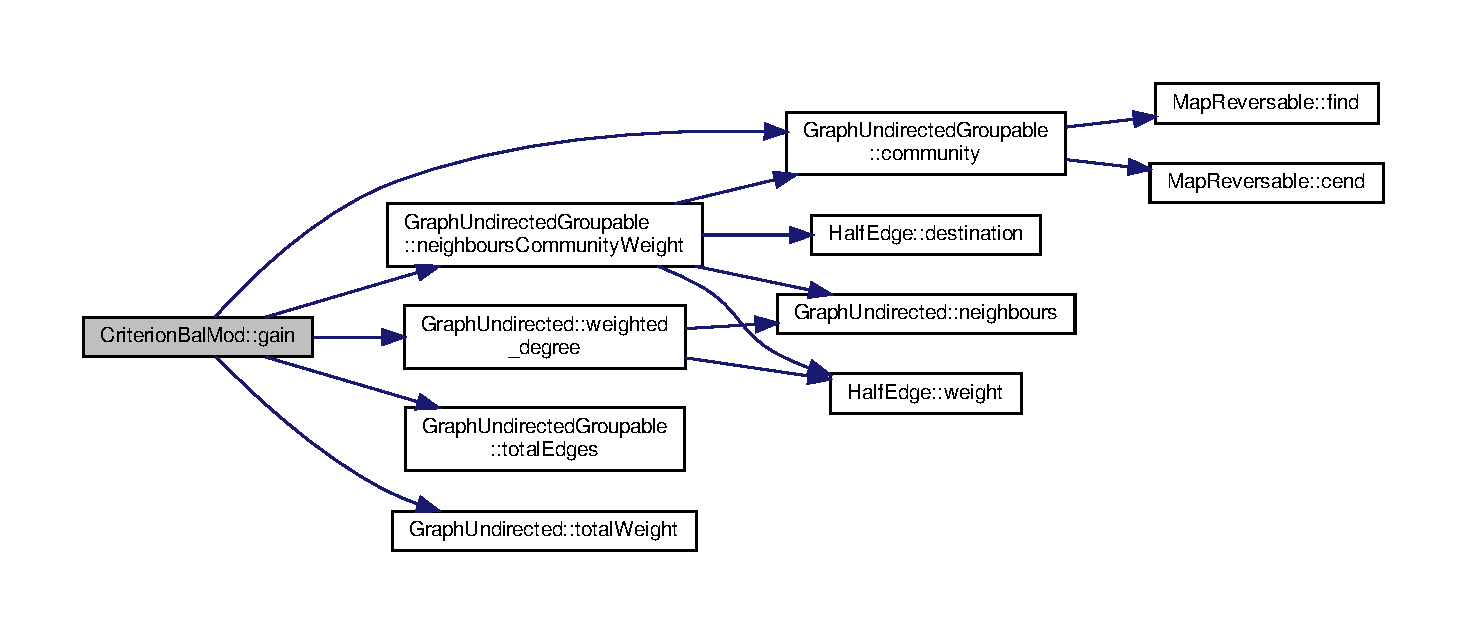
\includegraphics[width=350pt]{classCriterionBalMod_acf5001622eb8c495a5d5e8f044c22395_cgraph}
\end{center}
\end{figure}
\mbox{\Hypertarget{classCriterionBalMod_a87c0ccb5e2a851420dc82bd23cc31716}\label{classCriterionBalMod_a87c0ccb5e2a851420dc82bd23cc31716}} 
\index{Criterion\+Bal\+Mod@{Criterion\+Bal\+Mod}!quality@{quality}}
\index{quality@{quality}!Criterion\+Bal\+Mod@{Criterion\+Bal\+Mod}}
\subsubsection{\texorpdfstring{quality()}{quality()}}
{\footnotesize\ttfamily \hyperlink{criterionInterface_8h_af71ff22f6355fd69a4a62104bfd59a83}{type\+Criterion} Criterion\+Bal\+Mod\+::quality (\begin{DoxyParamCaption}{ }\end{DoxyParamCaption}) const\hspace{0.3cm}{\ttfamily [inline]}, {\ttfamily [virtual]}}

compute the quality of the current partition scheme

\begin{DoxyReturn}{Returns}
the quality value 
\end{DoxyReturn}


Implements \hyperlink{classCriterionInterface_a5d287dc7755f7ce7d6a3d91f0d8fa5de}{Criterion\+Interface}.



Definition at line 70 of file criterion\+Bal\+Mod.\+h.



References Criterion\+Base\+::g, Graph\+Undirected\+::get\+Vertices(), Graph\+Undirected\+Groupable\+::inner\+Edges(), Graph\+Undirected\+Groupable\+::total\+Edges(), and Graph\+Undirected\+::total\+Weight().



Referenced by Criterion\+::quality().

Here is the call graph for this function\+:
\nopagebreak
\begin{figure}[H]
\begin{center}
\leavevmode
\includegraphics[width=350pt]{classCriterionBalMod_a87c0ccb5e2a851420dc82bd23cc31716_cgraph}
\end{center}
\end{figure}


The documentation for this class was generated from the following file\+:\begin{DoxyCompactItemize}
\item 
R-\/\+C\+R\+A\+N/src/base/\+Cpp/\hyperlink{criterionBalMod_8h}{criterion\+Bal\+Mod.\+h}\end{DoxyCompactItemize}

\hypertarget{classCriterionBase}{}\section{Criterion\+Base Class Reference}
\label{classCriterionBase}\index{Criterion\+Base@{Criterion\+Base}}


Base class for criterion.  




{\ttfamily \#include $<$criterion\+Base.\+h$>$}



Inheritance diagram for Criterion\+Base\+:
\nopagebreak
\begin{figure}[H]
\begin{center}
\leavevmode
\includegraphics[width=282pt]{classCriterionBase__inherit__graph}
\end{center}
\end{figure}


Collaboration diagram for Criterion\+Base\+:
\nopagebreak
\begin{figure}[H]
\begin{center}
\leavevmode
\includegraphics[width=350pt]{classCriterionBase__coll__graph}
\end{center}
\end{figure}
\subsection*{Public Member Functions}
\begin{DoxyCompactItemize}
\item 
\hyperlink{classCriterionBase_a23370b412ce1e656415f77126e55f194}{Criterion\+Base} (const \hyperlink{classGraphUndirectedGroupable}{Graph\+Undirected\+Groupable} \&graph, const \hyperlink{structProgramParameters}{Program\+Parameters} \&parameters=\hyperlink{program_8h_ae2d819404495f80f31db7676c1329d19}{arguments\+Default})
\item 
virtual \hyperlink{classCriterionBase_a6787dc90e0ac605e3115949cb19f0867}{$\sim$\+Criterion\+Base} ()
\end{DoxyCompactItemize}
\subsection*{Protected Attributes}
\begin{DoxyCompactItemize}
\item 
const \hyperlink{classGraphUndirectedGroupable}{Graph\+Undirected\+Groupable} \& \hyperlink{classCriterionBase_a610fe9f207de420117ad25550c185f97}{g}
\item 
const \hyperlink{structProgramParameters}{Program\+Parameters} \& \hyperlink{classCriterionBase_a4253d177fc6e27cf675d541b116a1534}{prmtrs}
\end{DoxyCompactItemize}


\subsection{Detailed Description}
Base class for criterion. 

It simply stores references to the graph and program parameters objects.

This class should be extended by all criterion. It strengths the idea that those objects should not be copied and that the graph and program parameters should not be modified.

\begin{DoxyAuthor}{Author}
poltergeist0
\end{DoxyAuthor}
\begin{DoxyDate}{Date}
2018-\/08-\/19 
\end{DoxyDate}


Definition at line 45 of file criterion\+Base.\+h.



\subsection{Constructor \& Destructor Documentation}
\mbox{\Hypertarget{classCriterionBase_a23370b412ce1e656415f77126e55f194}\label{classCriterionBase_a23370b412ce1e656415f77126e55f194}} 
\index{Criterion\+Base@{Criterion\+Base}!Criterion\+Base@{Criterion\+Base}}
\index{Criterion\+Base@{Criterion\+Base}!Criterion\+Base@{Criterion\+Base}}
\subsubsection{\texorpdfstring{Criterion\+Base()}{CriterionBase()}}
{\footnotesize\ttfamily Criterion\+Base\+::\+Criterion\+Base (\begin{DoxyParamCaption}\item[{const \hyperlink{classGraphUndirectedGroupable}{Graph\+Undirected\+Groupable} \&}]{graph,  }\item[{const \hyperlink{structProgramParameters}{Program\+Parameters} \&}]{parameters = {\ttfamily \hyperlink{program_8h_ae2d819404495f80f31db7676c1329d19}{arguments\+Default}} }\end{DoxyParamCaption})\hspace{0.3cm}{\ttfamily [inline]}}

Constructor.


\begin{DoxyParams}{Parameters}
{\em graph} & reference to the graph object \\
\hline
{\em parameters} & reference to the parameters object \\
\hline
\end{DoxyParams}


Definition at line 58 of file criterion\+Base.\+h.

\mbox{\Hypertarget{classCriterionBase_a6787dc90e0ac605e3115949cb19f0867}\label{classCriterionBase_a6787dc90e0ac605e3115949cb19f0867}} 
\index{Criterion\+Base@{Criterion\+Base}!````~Criterion\+Base@{$\sim$\+Criterion\+Base}}
\index{````~Criterion\+Base@{$\sim$\+Criterion\+Base}!Criterion\+Base@{Criterion\+Base}}
\subsubsection{\texorpdfstring{$\sim$\+Criterion\+Base()}{~CriterionBase()}}
{\footnotesize\ttfamily virtual Criterion\+Base\+::$\sim$\+Criterion\+Base (\begin{DoxyParamCaption}{ }\end{DoxyParamCaption})\hspace{0.3cm}{\ttfamily [inline]}, {\ttfamily [virtual]}}

Destructor 

Definition at line 69 of file criterion\+Base.\+h.



\subsection{Member Data Documentation}
\mbox{\Hypertarget{classCriterionBase_a610fe9f207de420117ad25550c185f97}\label{classCriterionBase_a610fe9f207de420117ad25550c185f97}} 
\index{Criterion\+Base@{Criterion\+Base}!g@{g}}
\index{g@{g}!Criterion\+Base@{Criterion\+Base}}
\subsubsection{\texorpdfstring{g}{g}}
{\footnotesize\ttfamily const \hyperlink{classGraphUndirectedGroupable}{Graph\+Undirected\+Groupable}\& Criterion\+Base\+::g\hspace{0.3cm}{\ttfamily [protected]}}



Definition at line 47 of file criterion\+Base.\+h.



Referenced by Criterion\+Bal\+Mod\+::gain(), Criterion\+Modularity\+::gain(), Criterion\+Bal\+Mod\+::quality(), and Criterion\+Modularity\+::quality().

\mbox{\Hypertarget{classCriterionBase_a4253d177fc6e27cf675d541b116a1534}\label{classCriterionBase_a4253d177fc6e27cf675d541b116a1534}} 
\index{Criterion\+Base@{Criterion\+Base}!prmtrs@{prmtrs}}
\index{prmtrs@{prmtrs}!Criterion\+Base@{Criterion\+Base}}
\subsubsection{\texorpdfstring{prmtrs}{prmtrs}}
{\footnotesize\ttfamily const \hyperlink{structProgramParameters}{Program\+Parameters}\& Criterion\+Base\+::prmtrs\hspace{0.3cm}{\ttfamily [protected]}}



Definition at line 48 of file criterion\+Base.\+h.



The documentation for this class was generated from the following file\+:\begin{DoxyCompactItemize}
\item 
R-\/\+C\+R\+A\+N/src/base/\+Cpp/\hyperlink{criterionBase_8h}{criterion\+Base.\+h}\end{DoxyCompactItemize}

\hypertarget{classCriterionInterface}{}\section{Criterion\+Interface Class Reference}
\label{classCriterionInterface}\index{Criterion\+Interface@{Criterion\+Interface}}


\hyperlink{classCriterion}{Criterion} interface.  




{\ttfamily \#include $<$criterion\+Interface.\+h$>$}



Inheritance diagram for Criterion\+Interface\+:
\nopagebreak
\begin{figure}[H]
\begin{center}
\leavevmode
\includegraphics[width=294pt]{classCriterionInterface__inherit__graph}
\end{center}
\end{figure}
\subsection*{Public Member Functions}
\begin{DoxyCompactItemize}
\item 
virtual \hyperlink{classCriterionInterface_afe9cbd3c6f58b5c54828cbfdd6d9d48d}{$\sim$\+Criterion\+Interface} ()
\item 
virtual \hyperlink{criterionInterface_8h_af71ff22f6355fd69a4a62104bfd59a83}{type\+Criterion} \hyperlink{classCriterionInterface_aa0beec8287cd70e16c057e7995d0caca}{gain} (const \hyperlink{edge_8h_a5fbd20c46956d479cb10afc9855223f6}{type\+Vertex} \&vertex, const \hyperlink{graphUndirectedGroupable_8h_a914da95c9ea7f14f4b7f875c36818556}{type\+Community} \&comm) const =0
\item 
virtual \hyperlink{criterionInterface_8h_af71ff22f6355fd69a4a62104bfd59a83}{type\+Criterion} \hyperlink{classCriterionInterface_a5d287dc7755f7ce7d6a3d91f0d8fa5de}{quality} () const =0
\end{DoxyCompactItemize}


\subsection{Detailed Description}
\hyperlink{classCriterion}{Criterion} interface. 

All criterion must implement the functions defined in this class.

Also, at the end of this class, there is a comment with the skeleton of a constructor that must be defined in classes that implement this interface.

\begin{DoxyAuthor}{Author}
poltergeist0
\end{DoxyAuthor}
\begin{DoxyDate}{Date}
2018-\/08-\/19 
\end{DoxyDate}


Definition at line 57 of file criterion\+Interface.\+h.



\subsection{Constructor \& Destructor Documentation}
\mbox{\Hypertarget{classCriterionInterface_afe9cbd3c6f58b5c54828cbfdd6d9d48d}\label{classCriterionInterface_afe9cbd3c6f58b5c54828cbfdd6d9d48d}} 
\index{Criterion\+Interface@{Criterion\+Interface}!````~Criterion\+Interface@{$\sim$\+Criterion\+Interface}}
\index{````~Criterion\+Interface@{$\sim$\+Criterion\+Interface}!Criterion\+Interface@{Criterion\+Interface}}
\subsubsection{\texorpdfstring{$\sim$\+Criterion\+Interface()}{~CriterionInterface()}}
{\footnotesize\ttfamily virtual Criterion\+Interface\+::$\sim$\+Criterion\+Interface (\begin{DoxyParamCaption}{ }\end{DoxyParamCaption})\hspace{0.3cm}{\ttfamily [inline]}, {\ttfamily [virtual]}}



Definition at line 59 of file criterion\+Interface.\+h.



References gain(), and quality().

Here is the call graph for this function\+:
\nopagebreak
\begin{figure}[H]
\begin{center}
\leavevmode
\includegraphics[width=312pt]{classCriterionInterface_afe9cbd3c6f58b5c54828cbfdd6d9d48d_cgraph}
\end{center}
\end{figure}


\subsection{Member Function Documentation}
\mbox{\Hypertarget{classCriterionInterface_aa0beec8287cd70e16c057e7995d0caca}\label{classCriterionInterface_aa0beec8287cd70e16c057e7995d0caca}} 
\index{Criterion\+Interface@{Criterion\+Interface}!gain@{gain}}
\index{gain@{gain}!Criterion\+Interface@{Criterion\+Interface}}
\subsubsection{\texorpdfstring{gain()}{gain()}}
{\footnotesize\ttfamily virtual \hyperlink{criterionInterface_8h_af71ff22f6355fd69a4a62104bfd59a83}{type\+Criterion} Criterion\+Interface\+::gain (\begin{DoxyParamCaption}\item[{const \hyperlink{edge_8h_a5fbd20c46956d479cb10afc9855223f6}{type\+Vertex} \&}]{vertex,  }\item[{const \hyperlink{graphUndirectedGroupable_8h_a914da95c9ea7f14f4b7f875c36818556}{type\+Community} \&}]{comm }\end{DoxyParamCaption}) const\hspace{0.3cm}{\ttfamily [pure virtual]}}

compute the quality obtained if the given vertex was moved from its current community to the given community


\begin{DoxyParams}{Parameters}
{\em vertex} & \\
\hline
{\em comm} & new potential community for given vertex \\
\hline
\end{DoxyParams}
\begin{DoxyReturn}{Returns}
the quality, which may be positive or negative 
\end{DoxyReturn}


Implemented in \hyperlink{classCriterion_a99e23ddc517ca3f2ea4766a5b4be0e3e}{Criterion}, \hyperlink{classCriterionModularity_a181617050bab1eeaaf38b2ad30dcfc43}{Criterion\+Modularity}, and \hyperlink{classCriterionBalMod_acf5001622eb8c495a5d5e8f044c22395}{Criterion\+Bal\+Mod}.



Referenced by $\sim$\+Criterion\+Interface().

\mbox{\Hypertarget{classCriterionInterface_a5d287dc7755f7ce7d6a3d91f0d8fa5de}\label{classCriterionInterface_a5d287dc7755f7ce7d6a3d91f0d8fa5de}} 
\index{Criterion\+Interface@{Criterion\+Interface}!quality@{quality}}
\index{quality@{quality}!Criterion\+Interface@{Criterion\+Interface}}
\subsubsection{\texorpdfstring{quality()}{quality()}}
{\footnotesize\ttfamily virtual \hyperlink{criterionInterface_8h_af71ff22f6355fd69a4a62104bfd59a83}{type\+Criterion} Criterion\+Interface\+::quality (\begin{DoxyParamCaption}{ }\end{DoxyParamCaption}) const\hspace{0.3cm}{\ttfamily [pure virtual]}}

compute the quality of the current partition scheme

\begin{DoxyReturn}{Returns}
the quality value 
\end{DoxyReturn}


Implemented in \hyperlink{classCriterion_a1f8b3a7bf56b5434b04d5366d754d459}{Criterion}, \hyperlink{classCriterionModularity_adf9197fd4e5878ca86501447b1fba989}{Criterion\+Modularity}, and \hyperlink{classCriterionBalMod_a87c0ccb5e2a851420dc82bd23cc31716}{Criterion\+Bal\+Mod}.



Referenced by $\sim$\+Criterion\+Interface().



The documentation for this class was generated from the following file\+:\begin{DoxyCompactItemize}
\item 
R-\/\+C\+R\+A\+N/src/base/\+Cpp/\hyperlink{criterionInterface_8h}{criterion\+Interface.\+h}\end{DoxyCompactItemize}

\hypertarget{classCriterionModularity}{}\section{Criterion\+Modularity Class Reference}
\label{classCriterionModularity}\index{Criterion\+Modularity@{Criterion\+Modularity}}


Newman-\/\+Girvan criterion.  




{\ttfamily \#include $<$criterion\+Modularity.\+h$>$}



Inheritance diagram for Criterion\+Modularity\+:
\nopagebreak
\begin{figure}[H]
\begin{center}
\leavevmode
\includegraphics[width=178pt]{classCriterionModularity__inherit__graph}
\end{center}
\end{figure}


Collaboration diagram for Criterion\+Modularity\+:
\nopagebreak
\begin{figure}[H]
\begin{center}
\leavevmode
\includegraphics[width=350pt]{classCriterionModularity__coll__graph}
\end{center}
\end{figure}
\subsection*{Public Member Functions}
\begin{DoxyCompactItemize}
\item 
\hyperlink{classCriterionModularity_a10cef5036f6748045aa87295c4b9ab6c}{Criterion\+Modularity} (const \hyperlink{classGraphUndirectedGroupable}{Graph\+Undirected\+Groupable} \&graph, const \hyperlink{structProgramParameters}{Program\+Parameters} \&parameters=\hyperlink{program_8h_ae2d819404495f80f31db7676c1329d19}{arguments\+Default})
\item 
\hyperlink{classCriterionModularity_a37d3f5ffcf397ec89e63c24705860496}{$\sim$\+Criterion\+Modularity} ()
\item 
\hyperlink{criterionInterface_8h_af71ff22f6355fd69a4a62104bfd59a83}{type\+Criterion} \hyperlink{classCriterionModularity_a181617050bab1eeaaf38b2ad30dcfc43}{gain} (const \hyperlink{edge_8h_a5fbd20c46956d479cb10afc9855223f6}{type\+Vertex} \&vertex, const \hyperlink{graphUndirectedGroupable_8h_a914da95c9ea7f14f4b7f875c36818556}{type\+Community} \&comm) const
\item 
\hyperlink{criterionInterface_8h_af71ff22f6355fd69a4a62104bfd59a83}{type\+Criterion} \hyperlink{classCriterionModularity_adf9197fd4e5878ca86501447b1fba989}{quality} () const
\end{DoxyCompactItemize}
\subsection*{Additional Inherited Members}


\subsection{Detailed Description}
Newman-\/\+Girvan criterion. 

\begin{DoxyAuthor}{Author}
poltergeist0
\end{DoxyAuthor}
\begin{DoxyDate}{Date}
2018-\/08-\/20 
\end{DoxyDate}


Definition at line 31 of file criterion\+Modularity.\+h.



\subsection{Constructor \& Destructor Documentation}
\mbox{\Hypertarget{classCriterionModularity_a10cef5036f6748045aa87295c4b9ab6c}\label{classCriterionModularity_a10cef5036f6748045aa87295c4b9ab6c}} 
\index{Criterion\+Modularity@{Criterion\+Modularity}!Criterion\+Modularity@{Criterion\+Modularity}}
\index{Criterion\+Modularity@{Criterion\+Modularity}!Criterion\+Modularity@{Criterion\+Modularity}}
\subsubsection{\texorpdfstring{Criterion\+Modularity()}{CriterionModularity()}}
{\footnotesize\ttfamily Criterion\+Modularity\+::\+Criterion\+Modularity (\begin{DoxyParamCaption}\item[{const \hyperlink{classGraphUndirectedGroupable}{Graph\+Undirected\+Groupable} \&}]{graph,  }\item[{const \hyperlink{structProgramParameters}{Program\+Parameters} \&}]{parameters = {\ttfamily \hyperlink{program_8h_ae2d819404495f80f31db7676c1329d19}{arguments\+Default}} }\end{DoxyParamCaption})\hspace{0.3cm}{\ttfamily [inline]}}

Constructor.


\begin{DoxyParams}{Parameters}
{\em graph} & reference to the graph object \\
\hline
{\em parameters} & reference to the parameters object \\
\hline
\end{DoxyParams}


Definition at line 41 of file criterion\+Modularity.\+h.

\mbox{\Hypertarget{classCriterionModularity_a37d3f5ffcf397ec89e63c24705860496}\label{classCriterionModularity_a37d3f5ffcf397ec89e63c24705860496}} 
\index{Criterion\+Modularity@{Criterion\+Modularity}!````~Criterion\+Modularity@{$\sim$\+Criterion\+Modularity}}
\index{````~Criterion\+Modularity@{$\sim$\+Criterion\+Modularity}!Criterion\+Modularity@{Criterion\+Modularity}}
\subsubsection{\texorpdfstring{$\sim$\+Criterion\+Modularity()}{~CriterionModularity()}}
{\footnotesize\ttfamily Criterion\+Modularity\+::$\sim$\+Criterion\+Modularity (\begin{DoxyParamCaption}{ }\end{DoxyParamCaption})\hspace{0.3cm}{\ttfamily [inline]}}

Destructor 

Definition at line 46 of file criterion\+Modularity.\+h.



\subsection{Member Function Documentation}
\mbox{\Hypertarget{classCriterionModularity_a181617050bab1eeaaf38b2ad30dcfc43}\label{classCriterionModularity_a181617050bab1eeaaf38b2ad30dcfc43}} 
\index{Criterion\+Modularity@{Criterion\+Modularity}!gain@{gain}}
\index{gain@{gain}!Criterion\+Modularity@{Criterion\+Modularity}}
\subsubsection{\texorpdfstring{gain()}{gain()}}
{\footnotesize\ttfamily \hyperlink{criterionInterface_8h_af71ff22f6355fd69a4a62104bfd59a83}{type\+Criterion} Criterion\+Modularity\+::gain (\begin{DoxyParamCaption}\item[{const \hyperlink{edge_8h_a5fbd20c46956d479cb10afc9855223f6}{type\+Vertex} \&}]{vertex,  }\item[{const \hyperlink{graphUndirectedGroupable_8h_a914da95c9ea7f14f4b7f875c36818556}{type\+Community} \&}]{comm }\end{DoxyParamCaption}) const\hspace{0.3cm}{\ttfamily [inline]}, {\ttfamily [virtual]}}

compute the quality obtained if the given vertex was moved from its current community to the given community


\begin{DoxyParams}{Parameters}
{\em vertex} & \\
\hline
{\em comm} & new potential community for given vertex \\
\hline
\end{DoxyParams}
\begin{DoxyReturn}{Returns}
the quality, which may be positive or negative 
\end{DoxyReturn}


Implements \hyperlink{classCriterionInterface_aa0beec8287cd70e16c057e7995d0caca}{Criterion\+Interface}.



Definition at line 57 of file criterion\+Modularity.\+h.



References Graph\+Undirected\+Groupable\+::community(), Criterion\+Base\+::g, Graph\+Undirected\+Groupable\+::neighbours\+Community\+Weight(), Graph\+Undirected\+Groupable\+::total\+Edges(), Graph\+Undirected\+::total\+Weight(), and Graph\+Undirected\+::weighted\+\_\+degree().



Referenced by Criterion\+::gain().

Here is the call graph for this function\+:
\nopagebreak
\begin{figure}[H]
\begin{center}
\leavevmode
\includegraphics[width=350pt]{classCriterionModularity_a181617050bab1eeaaf38b2ad30dcfc43_cgraph}
\end{center}
\end{figure}
\mbox{\Hypertarget{classCriterionModularity_adf9197fd4e5878ca86501447b1fba989}\label{classCriterionModularity_adf9197fd4e5878ca86501447b1fba989}} 
\index{Criterion\+Modularity@{Criterion\+Modularity}!quality@{quality}}
\index{quality@{quality}!Criterion\+Modularity@{Criterion\+Modularity}}
\subsubsection{\texorpdfstring{quality()}{quality()}}
{\footnotesize\ttfamily \hyperlink{criterionInterface_8h_af71ff22f6355fd69a4a62104bfd59a83}{type\+Criterion} Criterion\+Modularity\+::quality (\begin{DoxyParamCaption}{ }\end{DoxyParamCaption}) const\hspace{0.3cm}{\ttfamily [inline]}, {\ttfamily [virtual]}}

compute the quality of the current partition scheme

\begin{DoxyReturn}{Returns}
the quality value 
\end{DoxyReturn}


Implements \hyperlink{classCriterionInterface_a5d287dc7755f7ce7d6a3d91f0d8fa5de}{Criterion\+Interface}.



Definition at line 74 of file criterion\+Modularity.\+h.



References Criterion\+Base\+::g, Graph\+Undirected\+::get\+Vertices(), Graph\+Undirected\+Groupable\+::inner\+Edges(), Graph\+Undirected\+Groupable\+::total\+Edges(), and Graph\+Undirected\+::total\+Weight().



Referenced by Criterion\+::quality().

Here is the call graph for this function\+:
\nopagebreak
\begin{figure}[H]
\begin{center}
\leavevmode
\includegraphics[width=350pt]{classCriterionModularity_adf9197fd4e5878ca86501447b1fba989_cgraph}
\end{center}
\end{figure}


The documentation for this class was generated from the following file\+:\begin{DoxyCompactItemize}
\item 
R-\/\+C\+R\+A\+N/src/base/\+Cpp/\hyperlink{criterionModularity_8h}{criterion\+Modularity.\+h}\end{DoxyCompactItemize}

\hypertarget{classDummyAlgorithm}{}\section{Dummy\+Algorithm Class Reference}
\label{classDummyAlgorithm}\index{Dummy\+Algorithm@{Dummy\+Algorithm}}


Inheritance diagram for Dummy\+Algorithm\+:\nopagebreak
\begin{figure}[H]
\begin{center}
\leavevmode
\includegraphics[width=172pt]{classDummyAlgorithm__inherit__graph}
\end{center}
\end{figure}


Collaboration diagram for Dummy\+Algorithm\+:\nopagebreak
\begin{figure}[H]
\begin{center}
\leavevmode
\includegraphics[width=172pt]{classDummyAlgorithm__coll__graph}
\end{center}
\end{figure}


\subsection{Detailed Description}


Definition at line 36 of file Dyn\+Comm\+Rcpp.\+cpp.



The documentation for this class was generated from the following file\+:\begin{DoxyCompactItemize}
\item 
R-\/\+C\+R\+A\+N/src/\hyperlink{DynCommRcpp_8cpp}{Dyn\+Comm\+Rcpp.\+cpp}\end{DoxyCompactItemize}

\hypertarget{classDummyEnum}{}\section{Dummy\+Enum Class Reference}
\label{classDummyEnum}\index{Dummy\+Enum@{Dummy\+Enum}}


Inheritance diagram for Dummy\+Enum\+:
\nopagebreak
\begin{figure}[H]
\begin{center}
\leavevmode
\includegraphics[width=272pt]{classDummyEnum__inherit__graph}
\end{center}
\end{figure}
\subsection*{Private Member Functions}
\begin{DoxyCompactItemize}
\item 
int \hyperlink{classDummyEnum_a527da769af75620d1443857d2f300433}{get\+\_\+x} ()
\end{DoxyCompactItemize}
\subsection*{Private Attributes}
\begin{DoxyCompactItemize}
\item 
int \hyperlink{classDummyEnum_a0ad78287e6a1d56038b13370f313946c}{x}
\end{DoxyCompactItemize}


\subsection{Detailed Description}
Dummy class used to implement Enumeration like variables and function parameters in R from C++. May be removed in the future when R starts supporting C++ class enumerations. 

Definition at line 31 of file Dyn\+Comm\+Rcpp.\+cpp.



\subsection{Member Function Documentation}
\mbox{\Hypertarget{classDummyEnum_a527da769af75620d1443857d2f300433}\label{classDummyEnum_a527da769af75620d1443857d2f300433}} 
\index{Dummy\+Enum@{Dummy\+Enum}!get\+\_\+x@{get\+\_\+x}}
\index{get\+\_\+x@{get\+\_\+x}!Dummy\+Enum@{Dummy\+Enum}}
\subsubsection{\texorpdfstring{get\+\_\+x()}{get\_x()}}
{\footnotesize\ttfamily int Dummy\+Enum\+::get\+\_\+x (\begin{DoxyParamCaption}{ }\end{DoxyParamCaption})\hspace{0.3cm}{\ttfamily [inline]}, {\ttfamily [private]}}



Definition at line 33 of file Dyn\+Comm\+Rcpp.\+cpp.



References x.



\subsection{Member Data Documentation}
\mbox{\Hypertarget{classDummyEnum_a0ad78287e6a1d56038b13370f313946c}\label{classDummyEnum_a0ad78287e6a1d56038b13370f313946c}} 
\index{Dummy\+Enum@{Dummy\+Enum}!x@{x}}
\index{x@{x}!Dummy\+Enum@{Dummy\+Enum}}
\subsubsection{\texorpdfstring{x}{x}}
{\footnotesize\ttfamily int Dummy\+Enum\+::x\hspace{0.3cm}{\ttfamily [private]}}



Definition at line 32 of file Dyn\+Comm\+Rcpp.\+cpp.



Referenced by get\+\_\+x().



The documentation for this class was generated from the following file\+:\begin{DoxyCompactItemize}
\item 
R-\/\+C\+R\+A\+N/src/\hyperlink{DynCommRcpp_8cpp}{Dyn\+Comm\+Rcpp.\+cpp}\end{DoxyCompactItemize}

\hypertarget{classDummyQuality}{}\section{Dummy\+Quality Class Reference}
\label{classDummyQuality}\index{Dummy\+Quality@{Dummy\+Quality}}


Inheritance diagram for Dummy\+Quality\+:\nopagebreak
\begin{figure}[H]
\begin{center}
\leavevmode
\includegraphics[width=162pt]{classDummyQuality__inherit__graph}
\end{center}
\end{figure}


Collaboration diagram for Dummy\+Quality\+:\nopagebreak
\begin{figure}[H]
\begin{center}
\leavevmode
\includegraphics[width=162pt]{classDummyQuality__coll__graph}
\end{center}
\end{figure}


\subsection{Detailed Description}


Definition at line 40 of file Dyn\+Comm\+Rcpp.\+cpp.



The documentation for this class was generated from the following file\+:\begin{DoxyCompactItemize}
\item 
R-\/\+C\+R\+A\+N/src/\hyperlink{DynCommRcpp_8cpp}{Dyn\+Comm\+Rcpp.\+cpp}\end{DoxyCompactItemize}

\hypertarget{classDynCommBase}{}\section{Dyn\+Comm\+Base Class Reference}
\label{classDynCommBase}\index{Dyn\+Comm\+Base@{Dyn\+Comm\+Base}}


Dynamic Communities base class.  




{\ttfamily \#include $<$Dyn\+Comm\+Base.\+h$>$}



Inheritance diagram for Dyn\+Comm\+Base\+:
\nopagebreak
\begin{figure}[H]
\begin{center}
\leavevmode
\includegraphics[width=205pt]{classDynCommBase__inherit__graph}
\end{center}
\end{figure}


Collaboration diagram for Dyn\+Comm\+Base\+:
\nopagebreak
\begin{figure}[H]
\begin{center}
\leavevmode
\includegraphics[width=350pt]{classDynCommBase__coll__graph}
\end{center}
\end{figure}
\subsection*{Public Member Functions}
\begin{DoxyCompactItemize}
\item 
\hyperlink{classDynCommBase_a69682c03778e2f5d6b52c8139b26f454}{Dyn\+Comm\+Base} ()=delete
\item 
\hyperlink{classDynCommBase_a3dd8b3480d39f8be793d64a312b4da87}{Dyn\+Comm\+Base} (\hyperlink{classAlgorithm_a38e19a8c3dc51b97563a34d9e59a748d}{Algorithm\+::\+A\+L\+G\+O\+R\+I\+T\+HM} algorithm=\hyperlink{classAlgorithm_a38e19a8c3dc51b97563a34d9e59a748dab77e66715d6be972cdbf6cc4d990e732}{Algorithm\+::\+A\+L\+G\+O\+R\+I\+T\+H\+M\+::\+L\+O\+U\+V\+A\+IN}, const \hyperlink{classCriterion_a55594c223ce0837b8319c46c66cb648f}{Criterion\+::\+C\+R\+I\+T\+E\+R\+I\+ON} \&\hyperlink{classDynCommBase_a316b2c63a025810211d205ef6bf1d06c}{quality}=\hyperlink{classCriterion_a55594c223ce0837b8319c46c66cb648fa2a7d416fbe43baf234420601ea73d946}{Criterion\+::\+C\+R\+I\+T\+E\+R\+I\+O\+N\+::\+M\+O\+D\+U\+L\+A\+R\+I\+TY}, \hyperlink{structProgramParameters}{Program\+Parameters} \&algorithm\+Parameters=\hyperlink{program_8h_ae2d819404495f80f31db7676c1329d19}{arguments\+Default})
\item 
bool \hyperlink{classDynCommBase_a85ff9898ef25b12f3e80842c7b2696fe}{add\+Remove\+Edges} (\hyperlink{classReaderInterface}{Reader\+Interface}$<$ \hyperlink{classEdge}{Edge} $>$ $\ast$reader)
\item 
\hyperlink{criterionInterface_8h_af71ff22f6355fd69a4a62104bfd59a83}{type\+Criterion} \hyperlink{classDynCommBase_a316b2c63a025810211d205ef6bf1d06c}{quality} () const
\item 
int \hyperlink{classDynCommBase_add5d1d59a3f20b4ba039342b31551fb3}{community\+Count} () const
\item 
\hyperlink{graphUndirectedGroupable_8h_ab79c7252155ca17cb49aa0b1fea30116}{type\+Communities} \hyperlink{classDynCommBase_a064d9909a91cfe25acf05e6bd1fc967d}{communities} () const
\item 
\hyperlink{edge_8h_a2e7ea3be891ac8b52f749ec73fee6dd2}{type\+Weight} \hyperlink{classDynCommBase_af95d4ab7f1814514fd5961900731ba12}{communities\+Edge\+Count} () const
\item 
\hyperlink{graphInterface_8h_ae8d27008f15586bbf419af7ad2e0a48a}{type\+Links\+Range\+Const} \hyperlink{classDynCommBase_aba6f1f0fdd67a1d7f546d63706a60cde}{community\+Neighbours} (\hyperlink{graphUndirectedGroupable_8h_a914da95c9ea7f14f4b7f875c36818556}{type\+Community} \hyperlink{classDynCommBase_a651753518a2de4ea52caea518e74d878}{community}) const
\item 
\hyperlink{edge_8h_a2e7ea3be891ac8b52f749ec73fee6dd2}{type\+Weight} \hyperlink{classDynCommBase_ada91e7e914eb8be7f8c25f4c0c81156a}{community\+Inner\+Edges\+Weight} (\hyperlink{graphUndirectedGroupable_8h_a914da95c9ea7f14f4b7f875c36818556}{type\+Community} \hyperlink{classDynCommBase_a651753518a2de4ea52caea518e74d878}{community}) const
\item 
\hyperlink{edge_8h_a2e7ea3be891ac8b52f749ec73fee6dd2}{type\+Weight} \hyperlink{classDynCommBase_a9e7f2493dd9f2381dbfbe94b91ac49f4}{community\+Total\+Weight} (\hyperlink{graphUndirectedGroupable_8h_a914da95c9ea7f14f4b7f875c36818556}{type\+Community} \hyperlink{classDynCommBase_a651753518a2de4ea52caea518e74d878}{community}) const
\item 
\hyperlink{edge_8h_a2e7ea3be891ac8b52f749ec73fee6dd2}{type\+Weight} \hyperlink{classDynCommBase_a1ef408ec71d82b008fc0229416c77b61}{community\+Edge\+Weight} (\hyperlink{graphUndirectedGroupable_8h_a914da95c9ea7f14f4b7f875c36818556}{type\+Community} source, \hyperlink{graphUndirectedGroupable_8h_a914da95c9ea7f14f4b7f875c36818556}{type\+Community} destination) const
\item 
int \hyperlink{classDynCommBase_ad02f1853b63e1ceaf24b05cfdbcf7a49}{community\+Vertex\+Count} (\hyperlink{graphUndirectedGroupable_8h_a914da95c9ea7f14f4b7f875c36818556}{type\+Community} \hyperlink{classDynCommBase_a651753518a2de4ea52caea518e74d878}{community}) const
\item 
\hyperlink{graphUndirectedGroupable_8h_a914da95c9ea7f14f4b7f875c36818556}{type\+Community} \hyperlink{classDynCommBase_a651753518a2de4ea52caea518e74d878}{community} (\hyperlink{edge_8h_a5fbd20c46956d479cb10afc9855223f6}{type\+Vertex} vertex) const
\item 
unsigned int \hyperlink{classDynCommBase_ae415f1a7792158845f69d6850b762d87}{vertex\+Count} () const
\item 
\hyperlink{graphInterface_8h_a21d54d8a139def524d3b0d6f71ec4974}{type\+Vertex\+List} \hyperlink{classDynCommBase_ae240fba572935f26a72f73e39e115169}{vertices} () const
\item 
\hyperlink{graphInterface_8h_a21d54d8a139def524d3b0d6f71ec4974}{type\+Vertex\+List} \hyperlink{classDynCommBase_ae56cd1fc5a69fcd4d0e0a073f3f2e36b}{vertices} (\hyperlink{graphUndirectedGroupable_8h_a914da95c9ea7f14f4b7f875c36818556}{type\+Community} \hyperlink{classDynCommBase_a651753518a2de4ea52caea518e74d878}{community}) const
\item 
\hyperlink{edge_8h_a2e7ea3be891ac8b52f749ec73fee6dd2}{type\+Weight} \hyperlink{classDynCommBase_a5f7d75431e0f774c1c92f096d6a7c429}{edge\+Count} () const
\item 
bool \hyperlink{classDynCommBase_a75ed5e0546d756a3b327f41e292620b2}{community\+Mapping} (\hyperlink{classWriterInterface}{Writer\+Interface} $\ast$writer, bool community\+First=true, bool differential=true) const
\item 
\hyperlink{graphInterface_8h_ae8d27008f15586bbf419af7ad2e0a48a}{type\+Links\+Range\+Const} \hyperlink{classDynCommBase_a3500faab82a0547422b2202b79f49718}{neighbours} (\hyperlink{edge_8h_a5fbd20c46956d479cb10afc9855223f6}{type\+Vertex} vertex) const
\begin{DoxyCompactList}\small\item\em Get the neighbours of a vertex. \end{DoxyCompactList}\item 
\hyperlink{edge_8h_a2e7ea3be891ac8b52f749ec73fee6dd2}{type\+Weight} \hyperlink{classDynCommBase_ae48a572da3c7b375429e96e717b15787}{weight} (const \hyperlink{edge_8h_a5fbd20c46956d479cb10afc9855223f6}{type\+Vertex} \&source, const \hyperlink{edge_8h_a5fbd20c46956d479cb10afc9855223f6}{type\+Vertex} \&destination) const
\item 
\hyperlink{systemDefines_8h_abc0f5bc07737e498f287334775dff2b6}{uint64} \hyperlink{classDynCommBase_a5b40eb14cef877fde1db8b6476f6a2ce}{time} (bool accumulated=true) const
\end{DoxyCompactItemize}
\subsection*{Private Attributes}
\begin{DoxyCompactItemize}
\item 
\hyperlink{classAlgorithm}{Algorithm} \hyperlink{classDynCommBase_a966f54b7ba340fa782146659998760ed}{algrthm}
\item 
\hyperlink{classGraphUndirectedGroupable}{Graph\+Undirected\+Groupable} \hyperlink{classDynCommBase_ae79d443436131554acb4b3ed24908701}{grph}
\item 
\hyperlink{classCriterion}{Criterion} \hyperlink{classDynCommBase_a6de9b4c868b4b8ca2923db6f6b1f08f7}{qlt}
\item 
\hyperlink{structProgramParameters}{Program\+Parameters} \hyperlink{classDynCommBase_a61a92fd07b37a8153fda9cfebd779dc4}{prmtrs}
\item 
\hyperlink{systemDefines_8h_abc0f5bc07737e498f287334775dff2b6}{uint64} \hyperlink{classDynCommBase_ac796111a001f3c815d4b72e66da47cc2}{time\+Total} =0
\item 
\hyperlink{systemDefines_8h_abc0f5bc07737e498f287334775dff2b6}{uint64} \hyperlink{classDynCommBase_a7795433997aa908ce2b8be2b3f15aba0}{time\+Start} =0
\item 
\hyperlink{systemDefines_8h_abc0f5bc07737e498f287334775dff2b6}{uint64} \hyperlink{classDynCommBase_ae63166e1cbb91574ff23e4c667fad445}{time\+Processing} =0
\item 
\hyperlink{graphUndirectedGroupable_8h_a8d8ff0ef0315e7cd3b62e467487cd0e1}{type\+Community\+List} \hyperlink{classDynCommBase_ac8cd68d0bff480bc59878668369aa2a5}{old\+Communities}
\end{DoxyCompactItemize}
\subsection*{Additional Inherited Members}


\subsection{Detailed Description}
Dynamic Communities base class. 

Simple class that only converts between data types and dispatches function calls to the correct object (graph, criterion or algorithm).

\begin{DoxyAuthor}{Author}
poltergeist0
\end{DoxyAuthor}
\begin{DoxyDate}{Date}
2019-\/02-\/02 
\end{DoxyDate}


Definition at line 42 of file Dyn\+Comm\+Base.\+h.



\subsection{Constructor \& Destructor Documentation}
\mbox{\Hypertarget{classDynCommBase_a69682c03778e2f5d6b52c8139b26f454}\label{classDynCommBase_a69682c03778e2f5d6b52c8139b26f454}} 
\index{Dyn\+Comm\+Base@{Dyn\+Comm\+Base}!Dyn\+Comm\+Base@{Dyn\+Comm\+Base}}
\index{Dyn\+Comm\+Base@{Dyn\+Comm\+Base}!Dyn\+Comm\+Base@{Dyn\+Comm\+Base}}
\subsubsection{\texorpdfstring{Dyn\+Comm\+Base()}{DynCommBase()}\hspace{0.1cm}{\footnotesize\ttfamily [1/2]}}
{\footnotesize\ttfamily Dyn\+Comm\+Base\+::\+Dyn\+Comm\+Base (\begin{DoxyParamCaption}{ }\end{DoxyParamCaption})\hspace{0.3cm}{\ttfamily [delete]}}

Default constructor not acceptable. Must be passed at least the chosen algorithm and the graph \mbox{\Hypertarget{classDynCommBase_a3dd8b3480d39f8be793d64a312b4da87}\label{classDynCommBase_a3dd8b3480d39f8be793d64a312b4da87}} 
\index{Dyn\+Comm\+Base@{Dyn\+Comm\+Base}!Dyn\+Comm\+Base@{Dyn\+Comm\+Base}}
\index{Dyn\+Comm\+Base@{Dyn\+Comm\+Base}!Dyn\+Comm\+Base@{Dyn\+Comm\+Base}}
\subsubsection{\texorpdfstring{Dyn\+Comm\+Base()}{DynCommBase()}\hspace{0.1cm}{\footnotesize\ttfamily [2/2]}}
{\footnotesize\ttfamily Dyn\+Comm\+Base\+::\+Dyn\+Comm\+Base (\begin{DoxyParamCaption}\item[{\hyperlink{classAlgorithm_a38e19a8c3dc51b97563a34d9e59a748d}{Algorithm\+::\+A\+L\+G\+O\+R\+I\+T\+HM}}]{algorithm = {\ttfamily \hyperlink{classAlgorithm_a38e19a8c3dc51b97563a34d9e59a748dab77e66715d6be972cdbf6cc4d990e732}{Algorithm\+::\+A\+L\+G\+O\+R\+I\+T\+H\+M\+::\+L\+O\+U\+V\+A\+IN}},  }\item[{const \hyperlink{classCriterion_a55594c223ce0837b8319c46c66cb648f}{Criterion\+::\+C\+R\+I\+T\+E\+R\+I\+ON} \&}]{quality = {\ttfamily \hyperlink{classCriterion_a55594c223ce0837b8319c46c66cb648fa2a7d416fbe43baf234420601ea73d946}{Criterion\+::\+C\+R\+I\+T\+E\+R\+I\+O\+N\+::\+M\+O\+D\+U\+L\+A\+R\+I\+TY}},  }\item[{\hyperlink{structProgramParameters}{Program\+Parameters} \&}]{algorithm\+Parameters = {\ttfamily \hyperlink{program_8h_ae2d819404495f80f31db7676c1329d19}{arguments\+Default}} }\end{DoxyParamCaption})\hspace{0.3cm}{\ttfamily [inline]}}

Constructor 

Definition at line 81 of file Dyn\+Comm\+Base.\+h.



\subsection{Member Function Documentation}
\mbox{\Hypertarget{classDynCommBase_a85ff9898ef25b12f3e80842c7b2696fe}\label{classDynCommBase_a85ff9898ef25b12f3e80842c7b2696fe}} 
\index{Dyn\+Comm\+Base@{Dyn\+Comm\+Base}!add\+Remove\+Edges@{add\+Remove\+Edges}}
\index{add\+Remove\+Edges@{add\+Remove\+Edges}!Dyn\+Comm\+Base@{Dyn\+Comm\+Base}}
\subsubsection{\texorpdfstring{add\+Remove\+Edges()}{addRemoveEdges()}}
{\footnotesize\ttfamily bool Dyn\+Comm\+Base\+::add\+Remove\+Edges (\begin{DoxyParamCaption}\item[{\hyperlink{classReaderInterface}{Reader\+Interface}$<$ \hyperlink{classEdge}{Edge} $>$ $\ast$}]{reader }\end{DoxyParamCaption})\hspace{0.3cm}{\ttfamily [inline]}, {\ttfamily [virtual]}}

Function to add and remove edges from the graph. Any edge with a weight different from zero is inserted. Any edge with a weight of exactly zero is removed. \begin{DoxyReturn}{Returns}
true if adding/removing succeeded 
\end{DoxyReturn}


Implements \hyperlink{classDynCommBaseInterface_a08720be341a0e75c3535749219f7377b}{Dyn\+Comm\+Base\+Interface}.



Definition at line 102 of file Dyn\+Comm\+Base.\+h.



References Map\+Reversable$<$ T, U $>$\+::add(), Algorithm\+::add\+Remove\+Edges(), Graph\+Undirected\+Groupable\+::community(), Time\+::current\+Time(), Graph\+Undirected\+::get\+Vertices(), time\+Processing, and time\+Start.



Referenced by Dyn\+Comm\+Rcpp\+::add\+Remove\+Edges\+File(), and Dyn\+Comm\+Rcpp\+::add\+Remove\+Edges\+Matrix().

Here is the call graph for this function\+:
\nopagebreak
\begin{figure}[H]
\begin{center}
\leavevmode
\includegraphics[width=350pt]{classDynCommBase_a85ff9898ef25b12f3e80842c7b2696fe_cgraph}
\end{center}
\end{figure}
\mbox{\Hypertarget{classDynCommBase_a064d9909a91cfe25acf05e6bd1fc967d}\label{classDynCommBase_a064d9909a91cfe25acf05e6bd1fc967d}} 
\index{Dyn\+Comm\+Base@{Dyn\+Comm\+Base}!communities@{communities}}
\index{communities@{communities}!Dyn\+Comm\+Base@{Dyn\+Comm\+Base}}
\subsubsection{\texorpdfstring{communities()}{communities()}}
{\footnotesize\ttfamily \hyperlink{graphUndirectedGroupable_8h_ab79c7252155ca17cb49aa0b1fea30116}{type\+Communities} Dyn\+Comm\+Base\+::communities (\begin{DoxyParamCaption}{ }\end{DoxyParamCaption}) const\hspace{0.3cm}{\ttfamily [inline]}, {\ttfamily [virtual]}}

\begin{DoxyReturn}{Returns}
the list of all existing communities 
\end{DoxyReturn}


Implements \hyperlink{classDynCommBaseInterface_aedba7e43ae301ab910340f1d766d1698}{Dyn\+Comm\+Base\+Interface}.



Definition at line 135 of file Dyn\+Comm\+Base.\+h.



References Graph\+Undirected\+Groupable\+::communities().



Referenced by Dyn\+Comm\+Rcpp\+::communities().

Here is the call graph for this function\+:
\nopagebreak
\begin{figure}[H]
\begin{center}
\leavevmode
\includegraphics[width=350pt]{classDynCommBase_a064d9909a91cfe25acf05e6bd1fc967d_cgraph}
\end{center}
\end{figure}
\mbox{\Hypertarget{classDynCommBase_af95d4ab7f1814514fd5961900731ba12}\label{classDynCommBase_af95d4ab7f1814514fd5961900731ba12}} 
\index{Dyn\+Comm\+Base@{Dyn\+Comm\+Base}!communities\+Edge\+Count@{communities\+Edge\+Count}}
\index{communities\+Edge\+Count@{communities\+Edge\+Count}!Dyn\+Comm\+Base@{Dyn\+Comm\+Base}}
\subsubsection{\texorpdfstring{communities\+Edge\+Count()}{communitiesEdgeCount()}}
{\footnotesize\ttfamily \hyperlink{edge_8h_a2e7ea3be891ac8b52f749ec73fee6dd2}{type\+Weight} Dyn\+Comm\+Base\+::communities\+Edge\+Count (\begin{DoxyParamCaption}{ }\end{DoxyParamCaption}) const\hspace{0.3cm}{\ttfamily [inline]}}

Get the number of community to community edges in the graph

\begin{DoxyReturn}{Returns}
the number of edges 
\end{DoxyReturn}


Definition at line 144 of file Dyn\+Comm\+Base.\+h.



References Graph\+Undirected\+Groupable\+::communities\+Edge\+Count().



Referenced by Dyn\+Comm\+Rcpp\+::communities\+Edge\+Count().

Here is the call graph for this function\+:
\nopagebreak
\begin{figure}[H]
\begin{center}
\leavevmode
\includegraphics[width=350pt]{classDynCommBase_af95d4ab7f1814514fd5961900731ba12_cgraph}
\end{center}
\end{figure}
\mbox{\Hypertarget{classDynCommBase_a651753518a2de4ea52caea518e74d878}\label{classDynCommBase_a651753518a2de4ea52caea518e74d878}} 
\index{Dyn\+Comm\+Base@{Dyn\+Comm\+Base}!community@{community}}
\index{community@{community}!Dyn\+Comm\+Base@{Dyn\+Comm\+Base}}
\subsubsection{\texorpdfstring{community()}{community()}}
{\footnotesize\ttfamily \hyperlink{graphUndirectedGroupable_8h_a914da95c9ea7f14f4b7f875c36818556}{type\+Community} Dyn\+Comm\+Base\+::community (\begin{DoxyParamCaption}\item[{\hyperlink{edge_8h_a5fbd20c46956d479cb10afc9855223f6}{type\+Vertex}}]{vertex }\end{DoxyParamCaption}) const\hspace{0.3cm}{\ttfamily [inline]}, {\ttfamily [virtual]}}


\begin{DoxyParams}{Parameters}
{\em node} & \\
\hline
\end{DoxyParams}
\begin{DoxyReturn}{Returns}
the community of the given vertex or a special community of no\+G\+Roup if the vertex does not exist 
\end{DoxyReturn}


Implements \hyperlink{classDynCommBaseInterface_a9453a177580033aa1d4d9f165350ceba}{Dyn\+Comm\+Base\+Interface}.



Definition at line 210 of file Dyn\+Comm\+Base.\+h.



References Graph\+Undirected\+Groupable\+::community().



Referenced by Dyn\+Comm\+Rcpp\+::community(), and Dyn\+Comm\+Rcpp\+::community\+Mapping\+Matrix().

Here is the call graph for this function\+:
\nopagebreak
\begin{figure}[H]
\begin{center}
\leavevmode
\includegraphics[width=350pt]{classDynCommBase_a651753518a2de4ea52caea518e74d878_cgraph}
\end{center}
\end{figure}
\mbox{\Hypertarget{classDynCommBase_add5d1d59a3f20b4ba039342b31551fb3}\label{classDynCommBase_add5d1d59a3f20b4ba039342b31551fb3}} 
\index{Dyn\+Comm\+Base@{Dyn\+Comm\+Base}!community\+Count@{community\+Count}}
\index{community\+Count@{community\+Count}!Dyn\+Comm\+Base@{Dyn\+Comm\+Base}}
\subsubsection{\texorpdfstring{community\+Count()}{communityCount()}}
{\footnotesize\ttfamily int Dyn\+Comm\+Base\+::community\+Count (\begin{DoxyParamCaption}{ }\end{DoxyParamCaption}) const\hspace{0.3cm}{\ttfamily [inline]}, {\ttfamily [virtual]}}

\begin{DoxyReturn}{Returns}
the number of existing communities 
\end{DoxyReturn}


Implements \hyperlink{classDynCommBaseInterface_aa61588ce385fd66855e17747cf188a85}{Dyn\+Comm\+Base\+Interface}.



Definition at line 128 of file Dyn\+Comm\+Base.\+h.



References Graph\+Undirected\+Groupable\+::community\+Count().



Referenced by Dyn\+Comm\+Rcpp\+::community\+Count().

Here is the call graph for this function\+:
\nopagebreak
\begin{figure}[H]
\begin{center}
\leavevmode
\includegraphics[width=350pt]{classDynCommBase_add5d1d59a3f20b4ba039342b31551fb3_cgraph}
\end{center}
\end{figure}
\mbox{\Hypertarget{classDynCommBase_a1ef408ec71d82b008fc0229416c77b61}\label{classDynCommBase_a1ef408ec71d82b008fc0229416c77b61}} 
\index{Dyn\+Comm\+Base@{Dyn\+Comm\+Base}!community\+Edge\+Weight@{community\+Edge\+Weight}}
\index{community\+Edge\+Weight@{community\+Edge\+Weight}!Dyn\+Comm\+Base@{Dyn\+Comm\+Base}}
\subsubsection{\texorpdfstring{community\+Edge\+Weight()}{communityEdgeWeight()}}
{\footnotesize\ttfamily \hyperlink{edge_8h_a2e7ea3be891ac8b52f749ec73fee6dd2}{type\+Weight} Dyn\+Comm\+Base\+::community\+Edge\+Weight (\begin{DoxyParamCaption}\item[{\hyperlink{graphUndirectedGroupable_8h_a914da95c9ea7f14f4b7f875c36818556}{type\+Community}}]{source,  }\item[{\hyperlink{graphUndirectedGroupable_8h_a914da95c9ea7f14f4b7f875c36818556}{type\+Community}}]{destination }\end{DoxyParamCaption}) const\hspace{0.3cm}{\ttfamily [inline]}, {\ttfamily [virtual]}}

Get the weight of the edge form by two communities


\begin{DoxyParams}{Parameters}
{\em source} & community \\
\hline
{\em destination} & community \\
\hline
\end{DoxyParams}
\begin{DoxyReturn}{Returns}
the weight of the edge 
\end{DoxyReturn}


Implements \hyperlink{classDynCommBaseInterface_a17c322600ba39050005153845dfd3021}{Dyn\+Comm\+Base\+Interface}.



Definition at line 186 of file Dyn\+Comm\+Base.\+h.



References Graph\+Undirected\+Groupable\+::weight\+Community().



Referenced by Dyn\+Comm\+Rcpp\+::community\+Edge\+Weight().

Here is the call graph for this function\+:
\nopagebreak
\begin{figure}[H]
\begin{center}
\leavevmode
\includegraphics[width=350pt]{classDynCommBase_a1ef408ec71d82b008fc0229416c77b61_cgraph}
\end{center}
\end{figure}
\mbox{\Hypertarget{classDynCommBase_ada91e7e914eb8be7f8c25f4c0c81156a}\label{classDynCommBase_ada91e7e914eb8be7f8c25f4c0c81156a}} 
\index{Dyn\+Comm\+Base@{Dyn\+Comm\+Base}!community\+Inner\+Edges\+Weight@{community\+Inner\+Edges\+Weight}}
\index{community\+Inner\+Edges\+Weight@{community\+Inner\+Edges\+Weight}!Dyn\+Comm\+Base@{Dyn\+Comm\+Base}}
\subsubsection{\texorpdfstring{community\+Inner\+Edges\+Weight()}{communityInnerEdgesWeight()}}
{\footnotesize\ttfamily \hyperlink{edge_8h_a2e7ea3be891ac8b52f749ec73fee6dd2}{type\+Weight} Dyn\+Comm\+Base\+::community\+Inner\+Edges\+Weight (\begin{DoxyParamCaption}\item[{\hyperlink{graphUndirectedGroupable_8h_a914da95c9ea7f14f4b7f875c36818556}{type\+Community}}]{community }\end{DoxyParamCaption}) const\hspace{0.3cm}{\ttfamily [inline]}, {\ttfamily [virtual]}}

Get the sum of the weights of all edges of the given community where both vertices of an edge belong to the given community.


\begin{DoxyParams}{Parameters}
{\em community} & \\
\hline
\end{DoxyParams}
\begin{DoxyReturn}{Returns}
the sum of the weights of all inner edges 
\end{DoxyReturn}


Implements \hyperlink{classDynCommBaseInterface_a0e68dcfcc55385ce60b000d76ccd2d86}{Dyn\+Comm\+Base\+Interface}.



Definition at line 165 of file Dyn\+Comm\+Base.\+h.



References Graph\+Undirected\+Groupable\+::inner\+Edges().



Referenced by Dyn\+Comm\+Rcpp\+::community\+Inner\+Edges\+Weight().

Here is the call graph for this function\+:
\nopagebreak
\begin{figure}[H]
\begin{center}
\leavevmode
\includegraphics[width=350pt]{classDynCommBase_ada91e7e914eb8be7f8c25f4c0c81156a_cgraph}
\end{center}
\end{figure}
\mbox{\Hypertarget{classDynCommBase_a75ed5e0546d756a3b327f41e292620b2}\label{classDynCommBase_a75ed5e0546d756a3b327f41e292620b2}} 
\index{Dyn\+Comm\+Base@{Dyn\+Comm\+Base}!community\+Mapping@{community\+Mapping}}
\index{community\+Mapping@{community\+Mapping}!Dyn\+Comm\+Base@{Dyn\+Comm\+Base}}
\subsubsection{\texorpdfstring{community\+Mapping()}{communityMapping()}}
{\footnotesize\ttfamily bool Dyn\+Comm\+Base\+::community\+Mapping (\begin{DoxyParamCaption}\item[{\hyperlink{classWriterInterface}{Writer\+Interface} $\ast$}]{writer,  }\item[{bool}]{community\+First = {\ttfamily true},  }\item[{bool}]{differential = {\ttfamily true} }\end{DoxyParamCaption}) const\hspace{0.3cm}{\ttfamily [inline]}, {\ttfamily [virtual]}}

Get a snapshot of the current community mapping. If community\+First is true the result will be one community per line with each line being a community followed by a list of vertices. If false, the result will be a vertex per line with each line being a single vertex and a single community. The differential parameter will probably be moved inside the writer as a parameter


\begin{DoxyParams}{Parameters}
{\em writer} & \\
\hline
{\em community\+First} & if true returns a community followed by a list of vertices, otherwise a vertex and its community \\
\hline
{\em differential} & return only what changed in the last iteration of the algorithm \\
\hline
\end{DoxyParams}
\begin{DoxyReturn}{Returns}
true if the operation succeeded 
\end{DoxyReturn}


Implements \hyperlink{classDynCommBaseInterface_a0985625f987f7f428d76f3baac54e398}{Dyn\+Comm\+Base\+Interface}.



Definition at line 263 of file Dyn\+Comm\+Base.\+h.



References Map\+Reversable$<$ T, U $>$\+::cbegin(), Map\+Reversable$<$ T, U $>$\+::cend(), Graph\+Undirected\+Groupable\+::communities(), Graph\+Undirected\+Groupable\+::community(), Graph\+Undirected\+::get\+Vertices(), Writer\+Interface\+::\+L\+I\+NE, Map\+Reversable$<$ T, U $>$\+::size(), Writer\+Interface\+::\+V\+A\+L\+UE, Map\+Reversable$<$ T, U $>$\+::value(), Graph\+Undirected\+::vertex\+Count(), vertices(), and Writer\+Interface\+::write().



Referenced by Dyn\+Comm\+Rcpp\+::community\+Mapping\+File().

Here is the call graph for this function\+:
\nopagebreak
\begin{figure}[H]
\begin{center}
\leavevmode
\includegraphics[width=350pt]{classDynCommBase_a75ed5e0546d756a3b327f41e292620b2_cgraph}
\end{center}
\end{figure}
\mbox{\Hypertarget{classDynCommBase_aba6f1f0fdd67a1d7f546d63706a60cde}\label{classDynCommBase_aba6f1f0fdd67a1d7f546d63706a60cde}} 
\index{Dyn\+Comm\+Base@{Dyn\+Comm\+Base}!community\+Neighbours@{community\+Neighbours}}
\index{community\+Neighbours@{community\+Neighbours}!Dyn\+Comm\+Base@{Dyn\+Comm\+Base}}
\subsubsection{\texorpdfstring{community\+Neighbours()}{communityNeighbours()}}
{\footnotesize\ttfamily \hyperlink{graphInterface_8h_ae8d27008f15586bbf419af7ad2e0a48a}{type\+Links\+Range\+Const} Dyn\+Comm\+Base\+::community\+Neighbours (\begin{DoxyParamCaption}\item[{\hyperlink{graphUndirectedGroupable_8h_a914da95c9ea7f14f4b7f875c36818556}{type\+Community}}]{community }\end{DoxyParamCaption}) const\hspace{0.3cm}{\ttfamily [inline]}, {\ttfamily [virtual]}}

Get the communities that are neighbours of the given community


\begin{DoxyParams}{Parameters}
{\em community} & \\
\hline
\end{DoxyParams}
\begin{DoxyReturn}{Returns}
the neighbouring communities 
\end{DoxyReturn}


Implements \hyperlink{classDynCommBaseInterface_afbae10b36098f57576378255d9c09faf}{Dyn\+Comm\+Base\+Interface}.



Definition at line 154 of file Dyn\+Comm\+Base.\+h.



References Graph\+Undirected\+Groupable\+::neighbouring\+Communities().



Referenced by Dyn\+Comm\+Rcpp\+::community\+Neighbours().

Here is the call graph for this function\+:
\nopagebreak
\begin{figure}[H]
\begin{center}
\leavevmode
\includegraphics[width=350pt]{classDynCommBase_aba6f1f0fdd67a1d7f546d63706a60cde_cgraph}
\end{center}
\end{figure}
\mbox{\Hypertarget{classDynCommBase_a9e7f2493dd9f2381dbfbe94b91ac49f4}\label{classDynCommBase_a9e7f2493dd9f2381dbfbe94b91ac49f4}} 
\index{Dyn\+Comm\+Base@{Dyn\+Comm\+Base}!community\+Total\+Weight@{community\+Total\+Weight}}
\index{community\+Total\+Weight@{community\+Total\+Weight}!Dyn\+Comm\+Base@{Dyn\+Comm\+Base}}
\subsubsection{\texorpdfstring{community\+Total\+Weight()}{communityTotalWeight()}}
{\footnotesize\ttfamily \hyperlink{edge_8h_a2e7ea3be891ac8b52f749ec73fee6dd2}{type\+Weight} Dyn\+Comm\+Base\+::community\+Total\+Weight (\begin{DoxyParamCaption}\item[{\hyperlink{graphUndirectedGroupable_8h_a914da95c9ea7f14f4b7f875c36818556}{type\+Community}}]{community }\end{DoxyParamCaption}) const\hspace{0.3cm}{\ttfamily [inline]}, {\ttfamily [virtual]}}

Get the sum of the weights of all edges of the given community.


\begin{DoxyParams}{Parameters}
{\em community} & \\
\hline
\end{DoxyParams}
\begin{DoxyReturn}{Returns}
the sum of the weights of all edges 
\end{DoxyReturn}


Implements \hyperlink{classDynCommBaseInterface_a06e0b8a06e9c1067e12f574458db3eb0}{Dyn\+Comm\+Base\+Interface}.



Definition at line 175 of file Dyn\+Comm\+Base.\+h.



References Graph\+Undirected\+Groupable\+::total\+Edges().



Referenced by Dyn\+Comm\+Rcpp\+::community\+Total\+Weight().

Here is the call graph for this function\+:
\nopagebreak
\begin{figure}[H]
\begin{center}
\leavevmode
\includegraphics[width=350pt]{classDynCommBase_a9e7f2493dd9f2381dbfbe94b91ac49f4_cgraph}
\end{center}
\end{figure}
\mbox{\Hypertarget{classDynCommBase_ad02f1853b63e1ceaf24b05cfdbcf7a49}\label{classDynCommBase_ad02f1853b63e1ceaf24b05cfdbcf7a49}} 
\index{Dyn\+Comm\+Base@{Dyn\+Comm\+Base}!community\+Vertex\+Count@{community\+Vertex\+Count}}
\index{community\+Vertex\+Count@{community\+Vertex\+Count}!Dyn\+Comm\+Base@{Dyn\+Comm\+Base}}
\subsubsection{\texorpdfstring{community\+Vertex\+Count()}{communityVertexCount()}}
{\footnotesize\ttfamily int Dyn\+Comm\+Base\+::community\+Vertex\+Count (\begin{DoxyParamCaption}\item[{\hyperlink{graphUndirectedGroupable_8h_a914da95c9ea7f14f4b7f875c36818556}{type\+Community}}]{community }\end{DoxyParamCaption}) const\hspace{0.3cm}{\ttfamily [inline]}, {\ttfamily [virtual]}}

Get the number of vertices in the given community


\begin{DoxyParams}{Parameters}
{\em community} & \\
\hline
\end{DoxyParams}
\begin{DoxyReturn}{Returns}
the number of vertices 
\end{DoxyReturn}


Implements \hyperlink{classDynCommBaseInterface_a2b4c4a130a2de5eb6cd79af88969ef3c}{Dyn\+Comm\+Base\+Interface}.



Definition at line 196 of file Dyn\+Comm\+Base.\+h.



References Graph\+Undirected\+Groupable\+::vertices().



Referenced by Dyn\+Comm\+Rcpp\+::community\+Vertex\+Count().

Here is the call graph for this function\+:
\nopagebreak
\begin{figure}[H]
\begin{center}
\leavevmode
\includegraphics[width=350pt]{classDynCommBase_ad02f1853b63e1ceaf24b05cfdbcf7a49_cgraph}
\end{center}
\end{figure}
\mbox{\Hypertarget{classDynCommBase_a5f7d75431e0f774c1c92f096d6a7c429}\label{classDynCommBase_a5f7d75431e0f774c1c92f096d6a7c429}} 
\index{Dyn\+Comm\+Base@{Dyn\+Comm\+Base}!edge\+Count@{edge\+Count}}
\index{edge\+Count@{edge\+Count}!Dyn\+Comm\+Base@{Dyn\+Comm\+Base}}
\subsubsection{\texorpdfstring{edge\+Count()}{edgeCount()}}
{\footnotesize\ttfamily \hyperlink{edge_8h_a2e7ea3be891ac8b52f749ec73fee6dd2}{type\+Weight} Dyn\+Comm\+Base\+::edge\+Count (\begin{DoxyParamCaption}{ }\end{DoxyParamCaption}) const\hspace{0.3cm}{\ttfamily [inline]}}

Get the number of vertex to vertex edges in the graph

\begin{DoxyReturn}{Returns}
the number of edges 
\end{DoxyReturn}


Definition at line 246 of file Dyn\+Comm\+Base.\+h.



References Graph\+Undirected\+::edge\+Count().



Referenced by Dyn\+Comm\+Rcpp\+::edge\+Count().

Here is the call graph for this function\+:
\nopagebreak
\begin{figure}[H]
\begin{center}
\leavevmode
\includegraphics[width=350pt]{classDynCommBase_a5f7d75431e0f774c1c92f096d6a7c429_cgraph}
\end{center}
\end{figure}
\mbox{\Hypertarget{classDynCommBase_a3500faab82a0547422b2202b79f49718}\label{classDynCommBase_a3500faab82a0547422b2202b79f49718}} 
\index{Dyn\+Comm\+Base@{Dyn\+Comm\+Base}!neighbours@{neighbours}}
\index{neighbours@{neighbours}!Dyn\+Comm\+Base@{Dyn\+Comm\+Base}}
\subsubsection{\texorpdfstring{neighbours()}{neighbours()}}
{\footnotesize\ttfamily \hyperlink{graphInterface_8h_ae8d27008f15586bbf419af7ad2e0a48a}{type\+Links\+Range\+Const} Dyn\+Comm\+Base\+::neighbours (\begin{DoxyParamCaption}\item[{\hyperlink{edge_8h_a5fbd20c46956d479cb10afc9855223f6}{type\+Vertex}}]{vertex }\end{DoxyParamCaption}) const\hspace{0.3cm}{\ttfamily [inline]}, {\ttfamily [virtual]}}



Get the neighbours of a vertex. 

The pair can change between calls if the Indexed edge list is modified. 
\begin{DoxyParams}{Parameters}
{\em vertex} & \\
\hline
\end{DoxyParams}
\begin{DoxyReturn}{Returns}
pointers to the first and last neighbour of the vertex 
\end{DoxyReturn}


Implements \hyperlink{classDynCommBaseInterface_a9d6f5345d8cdf9e0d70b7a71bff8ade6}{Dyn\+Comm\+Base\+Interface}.



Definition at line 394 of file Dyn\+Comm\+Base.\+h.



References Graph\+Undirected\+::neighbours().



Referenced by Dyn\+Comm\+Rcpp\+::neighbours().

Here is the call graph for this function\+:
\nopagebreak
\begin{figure}[H]
\begin{center}
\leavevmode
\includegraphics[width=350pt]{classDynCommBase_a3500faab82a0547422b2202b79f49718_cgraph}
\end{center}
\end{figure}
\mbox{\Hypertarget{classDynCommBase_a316b2c63a025810211d205ef6bf1d06c}\label{classDynCommBase_a316b2c63a025810211d205ef6bf1d06c}} 
\index{Dyn\+Comm\+Base@{Dyn\+Comm\+Base}!quality@{quality}}
\index{quality@{quality}!Dyn\+Comm\+Base@{Dyn\+Comm\+Base}}
\subsubsection{\texorpdfstring{quality()}{quality()}}
{\footnotesize\ttfamily \hyperlink{criterionInterface_8h_af71ff22f6355fd69a4a62104bfd59a83}{type\+Criterion} Dyn\+Comm\+Base\+::quality (\begin{DoxyParamCaption}{ }\end{DoxyParamCaption}) const\hspace{0.3cm}{\ttfamily [inline]}, {\ttfamily [virtual]}}

\begin{DoxyReturn}{Returns}
the current quality measure of the community mapping on the graph 
\end{DoxyReturn}


Implements \hyperlink{classDynCommBaseInterface_a42863260fe57e0982be227255d4f8464}{Dyn\+Comm\+Base\+Interface}.



Definition at line 121 of file Dyn\+Comm\+Base.\+h.



References Criterion\+::quality().



Referenced by Dyn\+Comm\+Rcpp\+::quality().

Here is the call graph for this function\+:
\nopagebreak
\begin{figure}[H]
\begin{center}
\leavevmode
\includegraphics[width=350pt]{classDynCommBase_a316b2c63a025810211d205ef6bf1d06c_cgraph}
\end{center}
\end{figure}
\mbox{\Hypertarget{classDynCommBase_a5b40eb14cef877fde1db8b6476f6a2ce}\label{classDynCommBase_a5b40eb14cef877fde1db8b6476f6a2ce}} 
\index{Dyn\+Comm\+Base@{Dyn\+Comm\+Base}!time@{time}}
\index{time@{time}!Dyn\+Comm\+Base@{Dyn\+Comm\+Base}}
\subsubsection{\texorpdfstring{time()}{time()}}
{\footnotesize\ttfamily \hyperlink{systemDefines_8h_abc0f5bc07737e498f287334775dff2b6}{uint64} Dyn\+Comm\+Base\+::time (\begin{DoxyParamCaption}\item[{bool}]{accumulated = {\ttfamily true} }\end{DoxyParamCaption}) const\hspace{0.3cm}{\ttfamily [inline]}, {\ttfamily [virtual]}}

\begin{DoxyReturn}{Returns}
the total processing time in nanoseconds 
\end{DoxyReturn}


Implements \hyperlink{classDynCommBaseInterface_a6fb483ffc71baf6f0d4f6a0371e34ca9}{Dyn\+Comm\+Base\+Interface}.



Definition at line 409 of file Dyn\+Comm\+Base.\+h.



References time\+Processing, and time\+Total.



Referenced by Dyn\+Comm\+Rcpp\+::results(), and Dyn\+Comm\+Rcpp\+::time().

\mbox{\Hypertarget{classDynCommBase_ae415f1a7792158845f69d6850b762d87}\label{classDynCommBase_ae415f1a7792158845f69d6850b762d87}} 
\index{Dyn\+Comm\+Base@{Dyn\+Comm\+Base}!vertex\+Count@{vertex\+Count}}
\index{vertex\+Count@{vertex\+Count}!Dyn\+Comm\+Base@{Dyn\+Comm\+Base}}
\subsubsection{\texorpdfstring{vertex\+Count()}{vertexCount()}}
{\footnotesize\ttfamily unsigned int Dyn\+Comm\+Base\+::vertex\+Count (\begin{DoxyParamCaption}{ }\end{DoxyParamCaption}) const\hspace{0.3cm}{\ttfamily [inline]}, {\ttfamily [virtual]}}

\begin{DoxyReturn}{Returns}
the number of vertices in the graph 
\end{DoxyReturn}


Implements \hyperlink{classDynCommBaseInterface_a792b9c74e55abbc48fbc078bc5fead0c}{Dyn\+Comm\+Base\+Interface}.



Definition at line 217 of file Dyn\+Comm\+Base.\+h.



References Graph\+Undirected\+::vertex\+Count().



Referenced by Dyn\+Comm\+Rcpp\+::community\+Mapping\+Matrix(), and Dyn\+Comm\+Rcpp\+::vertex\+Count().

Here is the call graph for this function\+:
\nopagebreak
\begin{figure}[H]
\begin{center}
\leavevmode
\includegraphics[width=350pt]{classDynCommBase_ae415f1a7792158845f69d6850b762d87_cgraph}
\end{center}
\end{figure}
\mbox{\Hypertarget{classDynCommBase_ae240fba572935f26a72f73e39e115169}\label{classDynCommBase_ae240fba572935f26a72f73e39e115169}} 
\index{Dyn\+Comm\+Base@{Dyn\+Comm\+Base}!vertices@{vertices}}
\index{vertices@{vertices}!Dyn\+Comm\+Base@{Dyn\+Comm\+Base}}
\subsubsection{\texorpdfstring{vertices()}{vertices()}\hspace{0.1cm}{\footnotesize\ttfamily [1/2]}}
{\footnotesize\ttfamily \hyperlink{graphInterface_8h_a21d54d8a139def524d3b0d6f71ec4974}{type\+Vertex\+List} Dyn\+Comm\+Base\+::vertices (\begin{DoxyParamCaption}{ }\end{DoxyParamCaption}) const\hspace{0.3cm}{\ttfamily [inline]}, {\ttfamily [virtual]}}

\begin{DoxyReturn}{Returns}
a constant set with all vertices 
\end{DoxyReturn}


Implements \hyperlink{classDynCommBaseInterface_af5023d7b81f4413cc8052df01067f71f}{Dyn\+Comm\+Base\+Interface}.



Definition at line 224 of file Dyn\+Comm\+Base.\+h.



References Graph\+Undirected\+::get\+Vertices().



Referenced by community\+Mapping(), Dyn\+Comm\+Rcpp\+::community\+Mapping\+Matrix(), Dyn\+Comm\+Rcpp\+::vertices(), and Dyn\+Comm\+Rcpp\+::vertices\+All().

Here is the call graph for this function\+:
\nopagebreak
\begin{figure}[H]
\begin{center}
\leavevmode
\includegraphics[width=350pt]{classDynCommBase_ae240fba572935f26a72f73e39e115169_cgraph}
\end{center}
\end{figure}
\mbox{\Hypertarget{classDynCommBase_ae56cd1fc5a69fcd4d0e0a073f3f2e36b}\label{classDynCommBase_ae56cd1fc5a69fcd4d0e0a073f3f2e36b}} 
\index{Dyn\+Comm\+Base@{Dyn\+Comm\+Base}!vertices@{vertices}}
\index{vertices@{vertices}!Dyn\+Comm\+Base@{Dyn\+Comm\+Base}}
\subsubsection{\texorpdfstring{vertices()}{vertices()}\hspace{0.1cm}{\footnotesize\ttfamily [2/2]}}
{\footnotesize\ttfamily \hyperlink{graphInterface_8h_a21d54d8a139def524d3b0d6f71ec4974}{type\+Vertex\+List} Dyn\+Comm\+Base\+::vertices (\begin{DoxyParamCaption}\item[{\hyperlink{graphUndirectedGroupable_8h_a914da95c9ea7f14f4b7f875c36818556}{type\+Community}}]{community }\end{DoxyParamCaption}) const\hspace{0.3cm}{\ttfamily [inline]}, {\ttfamily [virtual]}}

\begin{DoxyReturn}{Returns}
a list of all vertices belonging to the given community 
\end{DoxyReturn}


Implements \hyperlink{classDynCommBaseInterface_ab178106e07cf3ad86ce2deb17dd5666e}{Dyn\+Comm\+Base\+Interface}.



Definition at line 231 of file Dyn\+Comm\+Base.\+h.



References Graph\+Undirected\+Groupable\+::vertices().

Here is the call graph for this function\+:
\nopagebreak
\begin{figure}[H]
\begin{center}
\leavevmode
\includegraphics[width=350pt]{classDynCommBase_ae56cd1fc5a69fcd4d0e0a073f3f2e36b_cgraph}
\end{center}
\end{figure}
\mbox{\Hypertarget{classDynCommBase_ae48a572da3c7b375429e96e717b15787}\label{classDynCommBase_ae48a572da3c7b375429e96e717b15787}} 
\index{Dyn\+Comm\+Base@{Dyn\+Comm\+Base}!weight@{weight}}
\index{weight@{weight}!Dyn\+Comm\+Base@{Dyn\+Comm\+Base}}
\subsubsection{\texorpdfstring{weight()}{weight()}}
{\footnotesize\ttfamily \hyperlink{edge_8h_a2e7ea3be891ac8b52f749ec73fee6dd2}{type\+Weight} Dyn\+Comm\+Base\+::weight (\begin{DoxyParamCaption}\item[{const \hyperlink{edge_8h_a5fbd20c46956d479cb10afc9855223f6}{type\+Vertex} \&}]{source,  }\item[{const \hyperlink{edge_8h_a5fbd20c46956d479cb10afc9855223f6}{type\+Vertex} \&}]{destination }\end{DoxyParamCaption}) const\hspace{0.3cm}{\ttfamily [inline]}, {\ttfamily [virtual]}}

\begin{DoxyReturn}{Returns}
the weight of the edge 
\end{DoxyReturn}


Implements \hyperlink{classDynCommBaseInterface_a31514affa49ac05ccf3318b3558cf0b2}{Dyn\+Comm\+Base\+Interface}.



Definition at line 401 of file Dyn\+Comm\+Base.\+h.



References Graph\+Undirected\+::weight().



Referenced by Dyn\+Comm\+Rcpp\+::edge\+Weight().

Here is the call graph for this function\+:
\nopagebreak
\begin{figure}[H]
\begin{center}
\leavevmode
\includegraphics[width=350pt]{classDynCommBase_ae48a572da3c7b375429e96e717b15787_cgraph}
\end{center}
\end{figure}


\subsection{Member Data Documentation}
\mbox{\Hypertarget{classDynCommBase_a966f54b7ba340fa782146659998760ed}\label{classDynCommBase_a966f54b7ba340fa782146659998760ed}} 
\index{Dyn\+Comm\+Base@{Dyn\+Comm\+Base}!algrthm@{algrthm}}
\index{algrthm@{algrthm}!Dyn\+Comm\+Base@{Dyn\+Comm\+Base}}
\subsubsection{\texorpdfstring{algrthm}{algrthm}}
{\footnotesize\ttfamily \hyperlink{classAlgorithm}{Algorithm} Dyn\+Comm\+Base\+::algrthm\hspace{0.3cm}{\ttfamily [private]}}



Definition at line 44 of file Dyn\+Comm\+Base.\+h.

\mbox{\Hypertarget{classDynCommBase_ae79d443436131554acb4b3ed24908701}\label{classDynCommBase_ae79d443436131554acb4b3ed24908701}} 
\index{Dyn\+Comm\+Base@{Dyn\+Comm\+Base}!grph@{grph}}
\index{grph@{grph}!Dyn\+Comm\+Base@{Dyn\+Comm\+Base}}
\subsubsection{\texorpdfstring{grph}{grph}}
{\footnotesize\ttfamily \hyperlink{classGraphUndirectedGroupable}{Graph\+Undirected\+Groupable} Dyn\+Comm\+Base\+::grph\hspace{0.3cm}{\ttfamily [private]}}



Definition at line 45 of file Dyn\+Comm\+Base.\+h.

\mbox{\Hypertarget{classDynCommBase_ac8cd68d0bff480bc59878668369aa2a5}\label{classDynCommBase_ac8cd68d0bff480bc59878668369aa2a5}} 
\index{Dyn\+Comm\+Base@{Dyn\+Comm\+Base}!old\+Communities@{old\+Communities}}
\index{old\+Communities@{old\+Communities}!Dyn\+Comm\+Base@{Dyn\+Comm\+Base}}
\subsubsection{\texorpdfstring{old\+Communities}{oldCommunities}}
{\footnotesize\ttfamily \hyperlink{graphUndirectedGroupable_8h_a8d8ff0ef0315e7cd3b62e467487cd0e1}{type\+Community\+List} Dyn\+Comm\+Base\+::old\+Communities\hspace{0.3cm}{\ttfamily [private]}}



Definition at line 69 of file Dyn\+Comm\+Base.\+h.

\mbox{\Hypertarget{classDynCommBase_a61a92fd07b37a8153fda9cfebd779dc4}\label{classDynCommBase_a61a92fd07b37a8153fda9cfebd779dc4}} 
\index{Dyn\+Comm\+Base@{Dyn\+Comm\+Base}!prmtrs@{prmtrs}}
\index{prmtrs@{prmtrs}!Dyn\+Comm\+Base@{Dyn\+Comm\+Base}}
\subsubsection{\texorpdfstring{prmtrs}{prmtrs}}
{\footnotesize\ttfamily \hyperlink{structProgramParameters}{Program\+Parameters} Dyn\+Comm\+Base\+::prmtrs\hspace{0.3cm}{\ttfamily [private]}}



Definition at line 47 of file Dyn\+Comm\+Base.\+h.

\mbox{\Hypertarget{classDynCommBase_a6de9b4c868b4b8ca2923db6f6b1f08f7}\label{classDynCommBase_a6de9b4c868b4b8ca2923db6f6b1f08f7}} 
\index{Dyn\+Comm\+Base@{Dyn\+Comm\+Base}!qlt@{qlt}}
\index{qlt@{qlt}!Dyn\+Comm\+Base@{Dyn\+Comm\+Base}}
\subsubsection{\texorpdfstring{qlt}{qlt}}
{\footnotesize\ttfamily \hyperlink{classCriterion}{Criterion} Dyn\+Comm\+Base\+::qlt\hspace{0.3cm}{\ttfamily [private]}}



Definition at line 46 of file Dyn\+Comm\+Base.\+h.

\mbox{\Hypertarget{classDynCommBase_ae63166e1cbb91574ff23e4c667fad445}\label{classDynCommBase_ae63166e1cbb91574ff23e4c667fad445}} 
\index{Dyn\+Comm\+Base@{Dyn\+Comm\+Base}!time\+Processing@{time\+Processing}}
\index{time\+Processing@{time\+Processing}!Dyn\+Comm\+Base@{Dyn\+Comm\+Base}}
\subsubsection{\texorpdfstring{time\+Processing}{timeProcessing}}
{\footnotesize\ttfamily \hyperlink{systemDefines_8h_abc0f5bc07737e498f287334775dff2b6}{uint64} Dyn\+Comm\+Base\+::time\+Processing =0\hspace{0.3cm}{\ttfamily [private]}}

total time used for processing 

Definition at line 62 of file Dyn\+Comm\+Base.\+h.



Referenced by add\+Remove\+Edges(), and time().

\mbox{\Hypertarget{classDynCommBase_a7795433997aa908ce2b8be2b3f15aba0}\label{classDynCommBase_a7795433997aa908ce2b8be2b3f15aba0}} 
\index{Dyn\+Comm\+Base@{Dyn\+Comm\+Base}!time\+Start@{time\+Start}}
\index{time\+Start@{time\+Start}!Dyn\+Comm\+Base@{Dyn\+Comm\+Base}}
\subsubsection{\texorpdfstring{time\+Start}{timeStart}}
{\footnotesize\ttfamily \hyperlink{systemDefines_8h_abc0f5bc07737e498f287334775dff2b6}{uint64} Dyn\+Comm\+Base\+::time\+Start =0\hspace{0.3cm}{\ttfamily [private]}}

auxiliary time used to store the start time 

Definition at line 57 of file Dyn\+Comm\+Base.\+h.



Referenced by add\+Remove\+Edges().

\mbox{\Hypertarget{classDynCommBase_ac796111a001f3c815d4b72e66da47cc2}\label{classDynCommBase_ac796111a001f3c815d4b72e66da47cc2}} 
\index{Dyn\+Comm\+Base@{Dyn\+Comm\+Base}!time\+Total@{time\+Total}}
\index{time\+Total@{time\+Total}!Dyn\+Comm\+Base@{Dyn\+Comm\+Base}}
\subsubsection{\texorpdfstring{time\+Total}{timeTotal}}
{\footnotesize\ttfamily \hyperlink{systemDefines_8h_abc0f5bc07737e498f287334775dff2b6}{uint64} Dyn\+Comm\+Base\+::time\+Total =0\hspace{0.3cm}{\ttfamily [private]}}

total accumulated time used for processing 

Definition at line 52 of file Dyn\+Comm\+Base.\+h.



Referenced by time().



The documentation for this class was generated from the following file\+:\begin{DoxyCompactItemize}
\item 
R-\/\+C\+R\+A\+N/src/base/\+Cpp/\hyperlink{DynCommBase_8h}{Dyn\+Comm\+Base.\+h}\end{DoxyCompactItemize}

\hypertarget{classDynCommBaseInterface}{}\section{Dyn\+Comm\+Base\+Interface Class Reference}
\label{classDynCommBaseInterface}\index{Dyn\+Comm\+Base\+Interface@{Dyn\+Comm\+Base\+Interface}}


Interface for Dyn\+Comm.  




{\ttfamily \#include $<$Dyn\+Comm\+Base\+Interface.\+h$>$}



Inheritance diagram for Dyn\+Comm\+Base\+Interface\+:
\nopagebreak
\begin{figure}[H]
\begin{center}
\leavevmode
\includegraphics[width=205pt]{classDynCommBaseInterface__inherit__graph}
\end{center}
\end{figure}
\subsection*{Public Member Functions}
\begin{DoxyCompactItemize}
\item 
virtual \hyperlink{classDynCommBaseInterface_a1bc41ad0bdef6a4d8370ba640a271b33}{$\sim$\+Dyn\+Comm\+Base\+Interface} ()
\item 
virtual bool \hyperlink{classDynCommBaseInterface_a08720be341a0e75c3535749219f7377b}{add\+Remove\+Edges} (\hyperlink{DynCommBaseInterface_8h_a78c081a2dec12142bd4225d9ee662d82}{Reader\+Edge\+Base} $\ast$reader)=0
\item 
virtual \hyperlink{criterionInterface_8h_af71ff22f6355fd69a4a62104bfd59a83}{type\+Criterion} \hyperlink{classDynCommBaseInterface_a42863260fe57e0982be227255d4f8464}{quality} () const =0
\item 
virtual int \hyperlink{classDynCommBaseInterface_aa61588ce385fd66855e17747cf188a85}{community\+Count} () const =0
\item 
virtual \hyperlink{graphUndirectedGroupable_8h_ab79c7252155ca17cb49aa0b1fea30116}{type\+Communities} \hyperlink{classDynCommBaseInterface_aedba7e43ae301ab910340f1d766d1698}{communities} () const =0
\item 
virtual \hyperlink{graphInterface_8h_ae8d27008f15586bbf419af7ad2e0a48a}{type\+Links\+Range\+Const} \hyperlink{classDynCommBaseInterface_afbae10b36098f57576378255d9c09faf}{community\+Neighbours} (\hyperlink{graphUndirectedGroupable_8h_a914da95c9ea7f14f4b7f875c36818556}{type\+Community} \hyperlink{classDynCommBaseInterface_a9453a177580033aa1d4d9f165350ceba}{community}) const =0
\item 
virtual \hyperlink{edge_8h_a2e7ea3be891ac8b52f749ec73fee6dd2}{type\+Weight} \hyperlink{classDynCommBaseInterface_a0e68dcfcc55385ce60b000d76ccd2d86}{community\+Inner\+Edges\+Weight} (\hyperlink{graphUndirectedGroupable_8h_a914da95c9ea7f14f4b7f875c36818556}{type\+Community} \hyperlink{classDynCommBaseInterface_a9453a177580033aa1d4d9f165350ceba}{community}) const =0
\item 
virtual \hyperlink{edge_8h_a2e7ea3be891ac8b52f749ec73fee6dd2}{type\+Weight} \hyperlink{classDynCommBaseInterface_a06e0b8a06e9c1067e12f574458db3eb0}{community\+Total\+Weight} (\hyperlink{graphUndirectedGroupable_8h_a914da95c9ea7f14f4b7f875c36818556}{type\+Community} \hyperlink{classDynCommBaseInterface_a9453a177580033aa1d4d9f165350ceba}{community}) const =0
\item 
virtual \hyperlink{edge_8h_a2e7ea3be891ac8b52f749ec73fee6dd2}{type\+Weight} \hyperlink{classDynCommBaseInterface_a17c322600ba39050005153845dfd3021}{community\+Edge\+Weight} (\hyperlink{graphUndirectedGroupable_8h_a914da95c9ea7f14f4b7f875c36818556}{type\+Community} source, \hyperlink{graphUndirectedGroupable_8h_a914da95c9ea7f14f4b7f875c36818556}{type\+Community} destination) const =0
\item 
virtual int \hyperlink{classDynCommBaseInterface_a2b4c4a130a2de5eb6cd79af88969ef3c}{community\+Vertex\+Count} (\hyperlink{graphUndirectedGroupable_8h_a914da95c9ea7f14f4b7f875c36818556}{type\+Community} \hyperlink{classDynCommBaseInterface_a9453a177580033aa1d4d9f165350ceba}{community}) const =0
\item 
virtual \hyperlink{graphUndirectedGroupable_8h_a914da95c9ea7f14f4b7f875c36818556}{type\+Community} \hyperlink{classDynCommBaseInterface_a9453a177580033aa1d4d9f165350ceba}{community} (\hyperlink{edge_8h_a5fbd20c46956d479cb10afc9855223f6}{type\+Vertex} vertex) const =0
\item 
virtual unsigned int \hyperlink{classDynCommBaseInterface_a792b9c74e55abbc48fbc078bc5fead0c}{vertex\+Count} () const =0
\item 
virtual \hyperlink{graphInterface_8h_a21d54d8a139def524d3b0d6f71ec4974}{type\+Vertex\+List} \hyperlink{classDynCommBaseInterface_af5023d7b81f4413cc8052df01067f71f}{vertices} () const =0
\item 
virtual \hyperlink{graphInterface_8h_a21d54d8a139def524d3b0d6f71ec4974}{type\+Vertex\+List} \hyperlink{classDynCommBaseInterface_ab178106e07cf3ad86ce2deb17dd5666e}{vertices} (\hyperlink{graphUndirectedGroupable_8h_a914da95c9ea7f14f4b7f875c36818556}{type\+Community} \hyperlink{classDynCommBaseInterface_a9453a177580033aa1d4d9f165350ceba}{community}) const =0
\item 
virtual bool \hyperlink{classDynCommBaseInterface_a0985625f987f7f428d76f3baac54e398}{community\+Mapping} (\hyperlink{classWriterInterface}{Writer\+Interface} $\ast$writer, bool community\+First=true, bool differential=true) const =0
\item 
virtual \hyperlink{graphInterface_8h_ae8d27008f15586bbf419af7ad2e0a48a}{type\+Links\+Range\+Const} \hyperlink{classDynCommBaseInterface_a9d6f5345d8cdf9e0d70b7a71bff8ade6}{neighbours} (\hyperlink{edge_8h_a5fbd20c46956d479cb10afc9855223f6}{type\+Vertex} vertex) const =0
\item 
virtual \hyperlink{edge_8h_a2e7ea3be891ac8b52f749ec73fee6dd2}{type\+Weight} \hyperlink{classDynCommBaseInterface_a31514affa49ac05ccf3318b3558cf0b2}{weight} (const \hyperlink{edge_8h_a5fbd20c46956d479cb10afc9855223f6}{type\+Vertex} \&source, const \hyperlink{edge_8h_a5fbd20c46956d479cb10afc9855223f6}{type\+Vertex} \&destination) const =0
\item 
virtual \hyperlink{systemDefines_8h_abc0f5bc07737e498f287334775dff2b6}{uint64} \hyperlink{classDynCommBaseInterface_a6fb483ffc71baf6f0d4f6a0371e34ca9}{time} (bool accumulated=true) const =0
\end{DoxyCompactItemize}


\subsection{Detailed Description}
Interface for Dyn\+Comm. 

Class that defines the interface for Dyn\+Comm as seen by the user.

It has as base the interface of classes graph, criterion and algorithm.

\begin{DoxyAuthor}{Author}
poltergeist0
\end{DoxyAuthor}
\begin{DoxyDate}{Date}
2019-\/01-\/01 
\end{DoxyDate}


Definition at line 39 of file Dyn\+Comm\+Base\+Interface.\+h.



\subsection{Constructor \& Destructor Documentation}
\mbox{\Hypertarget{classDynCommBaseInterface_a1bc41ad0bdef6a4d8370ba640a271b33}\label{classDynCommBaseInterface_a1bc41ad0bdef6a4d8370ba640a271b33}} 
\index{Dyn\+Comm\+Base\+Interface@{Dyn\+Comm\+Base\+Interface}!````~Dyn\+Comm\+Base\+Interface@{$\sim$\+Dyn\+Comm\+Base\+Interface}}
\index{````~Dyn\+Comm\+Base\+Interface@{$\sim$\+Dyn\+Comm\+Base\+Interface}!Dyn\+Comm\+Base\+Interface@{Dyn\+Comm\+Base\+Interface}}
\subsubsection{\texorpdfstring{$\sim$\+Dyn\+Comm\+Base\+Interface()}{~DynCommBaseInterface()}}
{\footnotesize\ttfamily virtual Dyn\+Comm\+Base\+Interface\+::$\sim$\+Dyn\+Comm\+Base\+Interface (\begin{DoxyParamCaption}{ }\end{DoxyParamCaption})\hspace{0.3cm}{\ttfamily [inline]}, {\ttfamily [virtual]}}

Destructor 

Definition at line 44 of file Dyn\+Comm\+Base\+Interface.\+h.



References add\+Remove\+Edges(), communities(), community(), community\+Count(), community\+Edge\+Weight(), community\+Inner\+Edges\+Weight(), community\+Mapping(), community\+Neighbours(), community\+Total\+Weight(), community\+Vertex\+Count(), neighbours(), quality(), time(), vertex\+Count(), vertices(), and weight().

Here is the call graph for this function\+:
\nopagebreak
\begin{figure}[H]
\begin{center}
\leavevmode
\includegraphics[height=550pt]{classDynCommBaseInterface_a1bc41ad0bdef6a4d8370ba640a271b33_cgraph}
\end{center}
\end{figure}


\subsection{Member Function Documentation}
\mbox{\Hypertarget{classDynCommBaseInterface_a08720be341a0e75c3535749219f7377b}\label{classDynCommBaseInterface_a08720be341a0e75c3535749219f7377b}} 
\index{Dyn\+Comm\+Base\+Interface@{Dyn\+Comm\+Base\+Interface}!add\+Remove\+Edges@{add\+Remove\+Edges}}
\index{add\+Remove\+Edges@{add\+Remove\+Edges}!Dyn\+Comm\+Base\+Interface@{Dyn\+Comm\+Base\+Interface}}
\subsubsection{\texorpdfstring{add\+Remove\+Edges()}{addRemoveEdges()}}
{\footnotesize\ttfamily virtual bool Dyn\+Comm\+Base\+Interface\+::add\+Remove\+Edges (\begin{DoxyParamCaption}\item[{\hyperlink{DynCommBaseInterface_8h_a78c081a2dec12142bd4225d9ee662d82}{Reader\+Edge\+Base} $\ast$}]{reader }\end{DoxyParamCaption})\hspace{0.3cm}{\ttfamily [pure virtual]}}

Function to add and remove edges from the graph. Any edge with a weight different from zero is inserted. Any edge with a weight of exactly zero is removed.


\begin{DoxyParams}{Parameters}
{\em reader} & is a Reader object that is responsible for converting the required data from its original format to Edges \\
\hline
\end{DoxyParams}
\begin{DoxyReturn}{Returns}
true if adding/removing succeeded 
\end{DoxyReturn}


Implemented in \hyperlink{classDynCommBase_a85ff9898ef25b12f3e80842c7b2696fe}{Dyn\+Comm\+Base}.



Referenced by $\sim$\+Dyn\+Comm\+Base\+Interface().

\mbox{\Hypertarget{classDynCommBaseInterface_aedba7e43ae301ab910340f1d766d1698}\label{classDynCommBaseInterface_aedba7e43ae301ab910340f1d766d1698}} 
\index{Dyn\+Comm\+Base\+Interface@{Dyn\+Comm\+Base\+Interface}!communities@{communities}}
\index{communities@{communities}!Dyn\+Comm\+Base\+Interface@{Dyn\+Comm\+Base\+Interface}}
\subsubsection{\texorpdfstring{communities()}{communities()}}
{\footnotesize\ttfamily virtual \hyperlink{graphUndirectedGroupable_8h_ab79c7252155ca17cb49aa0b1fea30116}{type\+Communities} Dyn\+Comm\+Base\+Interface\+::communities (\begin{DoxyParamCaption}{ }\end{DoxyParamCaption}) const\hspace{0.3cm}{\ttfamily [pure virtual]}}

\begin{DoxyReturn}{Returns}
the list of all existing communities without any further information 
\end{DoxyReturn}


Implemented in \hyperlink{classDynCommBase_a064d9909a91cfe25acf05e6bd1fc967d}{Dyn\+Comm\+Base}.



Referenced by $\sim$\+Dyn\+Comm\+Base\+Interface().

\mbox{\Hypertarget{classDynCommBaseInterface_a9453a177580033aa1d4d9f165350ceba}\label{classDynCommBaseInterface_a9453a177580033aa1d4d9f165350ceba}} 
\index{Dyn\+Comm\+Base\+Interface@{Dyn\+Comm\+Base\+Interface}!community@{community}}
\index{community@{community}!Dyn\+Comm\+Base\+Interface@{Dyn\+Comm\+Base\+Interface}}
\subsubsection{\texorpdfstring{community()}{community()}}
{\footnotesize\ttfamily virtual \hyperlink{graphUndirectedGroupable_8h_a914da95c9ea7f14f4b7f875c36818556}{type\+Community} Dyn\+Comm\+Base\+Interface\+::community (\begin{DoxyParamCaption}\item[{\hyperlink{edge_8h_a5fbd20c46956d479cb10afc9855223f6}{type\+Vertex}}]{vertex }\end{DoxyParamCaption}) const\hspace{0.3cm}{\ttfamily [pure virtual]}}


\begin{DoxyParams}{Parameters}
{\em vertex} & \\
\hline
\end{DoxyParams}
\begin{DoxyReturn}{Returns}
the community of a given vertex 
\end{DoxyReturn}


Implemented in \hyperlink{classDynCommBase_a651753518a2de4ea52caea518e74d878}{Dyn\+Comm\+Base}.



Referenced by $\sim$\+Dyn\+Comm\+Base\+Interface().

\mbox{\Hypertarget{classDynCommBaseInterface_aa61588ce385fd66855e17747cf188a85}\label{classDynCommBaseInterface_aa61588ce385fd66855e17747cf188a85}} 
\index{Dyn\+Comm\+Base\+Interface@{Dyn\+Comm\+Base\+Interface}!community\+Count@{community\+Count}}
\index{community\+Count@{community\+Count}!Dyn\+Comm\+Base\+Interface@{Dyn\+Comm\+Base\+Interface}}
\subsubsection{\texorpdfstring{community\+Count()}{communityCount()}}
{\footnotesize\ttfamily virtual int Dyn\+Comm\+Base\+Interface\+::community\+Count (\begin{DoxyParamCaption}{ }\end{DoxyParamCaption}) const\hspace{0.3cm}{\ttfamily [pure virtual]}}

\begin{DoxyReturn}{Returns}
the number of communities 
\end{DoxyReturn}


Implemented in \hyperlink{classDynCommBase_add5d1d59a3f20b4ba039342b31551fb3}{Dyn\+Comm\+Base}.



Referenced by $\sim$\+Dyn\+Comm\+Base\+Interface().

\mbox{\Hypertarget{classDynCommBaseInterface_a17c322600ba39050005153845dfd3021}\label{classDynCommBaseInterface_a17c322600ba39050005153845dfd3021}} 
\index{Dyn\+Comm\+Base\+Interface@{Dyn\+Comm\+Base\+Interface}!community\+Edge\+Weight@{community\+Edge\+Weight}}
\index{community\+Edge\+Weight@{community\+Edge\+Weight}!Dyn\+Comm\+Base\+Interface@{Dyn\+Comm\+Base\+Interface}}
\subsubsection{\texorpdfstring{community\+Edge\+Weight()}{communityEdgeWeight()}}
{\footnotesize\ttfamily virtual \hyperlink{edge_8h_a2e7ea3be891ac8b52f749ec73fee6dd2}{type\+Weight} Dyn\+Comm\+Base\+Interface\+::community\+Edge\+Weight (\begin{DoxyParamCaption}\item[{\hyperlink{graphUndirectedGroupable_8h_a914da95c9ea7f14f4b7f875c36818556}{type\+Community}}]{source,  }\item[{\hyperlink{graphUndirectedGroupable_8h_a914da95c9ea7f14f4b7f875c36818556}{type\+Community}}]{destination }\end{DoxyParamCaption}) const\hspace{0.3cm}{\ttfamily [pure virtual]}}


\begin{DoxyParams}{Parameters}
{\em source} & \\
\hline
{\em destination} & \\
\hline
\end{DoxyParams}
\begin{DoxyReturn}{Returns}
the weight of the edge that connects two given communities 
\end{DoxyReturn}


Implemented in \hyperlink{classDynCommBase_a1ef408ec71d82b008fc0229416c77b61}{Dyn\+Comm\+Base}.



Referenced by $\sim$\+Dyn\+Comm\+Base\+Interface().

\mbox{\Hypertarget{classDynCommBaseInterface_a0e68dcfcc55385ce60b000d76ccd2d86}\label{classDynCommBaseInterface_a0e68dcfcc55385ce60b000d76ccd2d86}} 
\index{Dyn\+Comm\+Base\+Interface@{Dyn\+Comm\+Base\+Interface}!community\+Inner\+Edges\+Weight@{community\+Inner\+Edges\+Weight}}
\index{community\+Inner\+Edges\+Weight@{community\+Inner\+Edges\+Weight}!Dyn\+Comm\+Base\+Interface@{Dyn\+Comm\+Base\+Interface}}
\subsubsection{\texorpdfstring{community\+Inner\+Edges\+Weight()}{communityInnerEdgesWeight()}}
{\footnotesize\ttfamily virtual \hyperlink{edge_8h_a2e7ea3be891ac8b52f749ec73fee6dd2}{type\+Weight} Dyn\+Comm\+Base\+Interface\+::community\+Inner\+Edges\+Weight (\begin{DoxyParamCaption}\item[{\hyperlink{graphUndirectedGroupable_8h_a914da95c9ea7f14f4b7f875c36818556}{type\+Community}}]{community }\end{DoxyParamCaption}) const\hspace{0.3cm}{\ttfamily [pure virtual]}}


\begin{DoxyParams}{Parameters}
{\em community} & \\
\hline
\end{DoxyParams}
\begin{DoxyReturn}{Returns}
the sum of the weights of all inner edges of the selected community 
\end{DoxyReturn}


Implemented in \hyperlink{classDynCommBase_ada91e7e914eb8be7f8c25f4c0c81156a}{Dyn\+Comm\+Base}.



Referenced by $\sim$\+Dyn\+Comm\+Base\+Interface().

\mbox{\Hypertarget{classDynCommBaseInterface_a0985625f987f7f428d76f3baac54e398}\label{classDynCommBaseInterface_a0985625f987f7f428d76f3baac54e398}} 
\index{Dyn\+Comm\+Base\+Interface@{Dyn\+Comm\+Base\+Interface}!community\+Mapping@{community\+Mapping}}
\index{community\+Mapping@{community\+Mapping}!Dyn\+Comm\+Base\+Interface@{Dyn\+Comm\+Base\+Interface}}
\subsubsection{\texorpdfstring{community\+Mapping()}{communityMapping()}}
{\footnotesize\ttfamily virtual bool Dyn\+Comm\+Base\+Interface\+::community\+Mapping (\begin{DoxyParamCaption}\item[{\hyperlink{classWriterInterface}{Writer\+Interface} $\ast$}]{writer,  }\item[{bool}]{community\+First = {\ttfamily true},  }\item[{bool}]{differential = {\ttfamily true} }\end{DoxyParamCaption}) const\hspace{0.3cm}{\ttfamily [pure virtual]}}

Get a snapshot of the current community mapping. If community\+First is true the result will be one community per line with each line being a community followed by a list of vertices. If false, the result will be a vertex per line with each line being a single vertex and a single community. The differential parameter will probably be moved inside the writer as a parameter


\begin{DoxyParams}{Parameters}
{\em writer} & \\
\hline
{\em community\+First} & if true returns a community followed by a list of vertices, otherwise a vertex and its community \\
\hline
{\em differential} & return only what changed in the last iteration of the algorithm \\
\hline
\end{DoxyParams}
\begin{DoxyReturn}{Returns}
true if the operation succeeded 
\end{DoxyReturn}


Implemented in \hyperlink{classDynCommBase_a75ed5e0546d756a3b327f41e292620b2}{Dyn\+Comm\+Base}.



Referenced by $\sim$\+Dyn\+Comm\+Base\+Interface().

\mbox{\Hypertarget{classDynCommBaseInterface_afbae10b36098f57576378255d9c09faf}\label{classDynCommBaseInterface_afbae10b36098f57576378255d9c09faf}} 
\index{Dyn\+Comm\+Base\+Interface@{Dyn\+Comm\+Base\+Interface}!community\+Neighbours@{community\+Neighbours}}
\index{community\+Neighbours@{community\+Neighbours}!Dyn\+Comm\+Base\+Interface@{Dyn\+Comm\+Base\+Interface}}
\subsubsection{\texorpdfstring{community\+Neighbours()}{communityNeighbours()}}
{\footnotesize\ttfamily virtual \hyperlink{graphInterface_8h_ae8d27008f15586bbf419af7ad2e0a48a}{type\+Links\+Range\+Const} Dyn\+Comm\+Base\+Interface\+::community\+Neighbours (\begin{DoxyParamCaption}\item[{\hyperlink{graphUndirectedGroupable_8h_a914da95c9ea7f14f4b7f875c36818556}{type\+Community}}]{community }\end{DoxyParamCaption}) const\hspace{0.3cm}{\ttfamily [pure virtual]}}


\begin{DoxyParams}{Parameters}
{\em community} & \\
\hline
\end{DoxyParams}
\begin{DoxyReturn}{Returns}
the neighboring communities of the given community 
\end{DoxyReturn}


Implemented in \hyperlink{classDynCommBase_aba6f1f0fdd67a1d7f546d63706a60cde}{Dyn\+Comm\+Base}.



Referenced by $\sim$\+Dyn\+Comm\+Base\+Interface().

\mbox{\Hypertarget{classDynCommBaseInterface_a06e0b8a06e9c1067e12f574458db3eb0}\label{classDynCommBaseInterface_a06e0b8a06e9c1067e12f574458db3eb0}} 
\index{Dyn\+Comm\+Base\+Interface@{Dyn\+Comm\+Base\+Interface}!community\+Total\+Weight@{community\+Total\+Weight}}
\index{community\+Total\+Weight@{community\+Total\+Weight}!Dyn\+Comm\+Base\+Interface@{Dyn\+Comm\+Base\+Interface}}
\subsubsection{\texorpdfstring{community\+Total\+Weight()}{communityTotalWeight()}}
{\footnotesize\ttfamily virtual \hyperlink{edge_8h_a2e7ea3be891ac8b52f749ec73fee6dd2}{type\+Weight} Dyn\+Comm\+Base\+Interface\+::community\+Total\+Weight (\begin{DoxyParamCaption}\item[{\hyperlink{graphUndirectedGroupable_8h_a914da95c9ea7f14f4b7f875c36818556}{type\+Community}}]{community }\end{DoxyParamCaption}) const\hspace{0.3cm}{\ttfamily [pure virtual]}}


\begin{DoxyParams}{Parameters}
{\em community} & \\
\hline
\end{DoxyParams}
\begin{DoxyReturn}{Returns}
the sum of the weights of all edges of the selected community 
\end{DoxyReturn}


Implemented in \hyperlink{classDynCommBase_a9e7f2493dd9f2381dbfbe94b91ac49f4}{Dyn\+Comm\+Base}.



Referenced by $\sim$\+Dyn\+Comm\+Base\+Interface().

\mbox{\Hypertarget{classDynCommBaseInterface_a2b4c4a130a2de5eb6cd79af88969ef3c}\label{classDynCommBaseInterface_a2b4c4a130a2de5eb6cd79af88969ef3c}} 
\index{Dyn\+Comm\+Base\+Interface@{Dyn\+Comm\+Base\+Interface}!community\+Vertex\+Count@{community\+Vertex\+Count}}
\index{community\+Vertex\+Count@{community\+Vertex\+Count}!Dyn\+Comm\+Base\+Interface@{Dyn\+Comm\+Base\+Interface}}
\subsubsection{\texorpdfstring{community\+Vertex\+Count()}{communityVertexCount()}}
{\footnotesize\ttfamily virtual int Dyn\+Comm\+Base\+Interface\+::community\+Vertex\+Count (\begin{DoxyParamCaption}\item[{\hyperlink{graphUndirectedGroupable_8h_a914da95c9ea7f14f4b7f875c36818556}{type\+Community}}]{community }\end{DoxyParamCaption}) const\hspace{0.3cm}{\ttfamily [pure virtual]}}


\begin{DoxyParams}{Parameters}
{\em community} & \\
\hline
\end{DoxyParams}
\begin{DoxyReturn}{Returns}
the amount of vertices in the selected community 
\end{DoxyReturn}


Implemented in \hyperlink{classDynCommBase_ad02f1853b63e1ceaf24b05cfdbcf7a49}{Dyn\+Comm\+Base}.



Referenced by $\sim$\+Dyn\+Comm\+Base\+Interface().

\mbox{\Hypertarget{classDynCommBaseInterface_a9d6f5345d8cdf9e0d70b7a71bff8ade6}\label{classDynCommBaseInterface_a9d6f5345d8cdf9e0d70b7a71bff8ade6}} 
\index{Dyn\+Comm\+Base\+Interface@{Dyn\+Comm\+Base\+Interface}!neighbours@{neighbours}}
\index{neighbours@{neighbours}!Dyn\+Comm\+Base\+Interface@{Dyn\+Comm\+Base\+Interface}}
\subsubsection{\texorpdfstring{neighbours()}{neighbours()}}
{\footnotesize\ttfamily virtual \hyperlink{graphInterface_8h_ae8d27008f15586bbf419af7ad2e0a48a}{type\+Links\+Range\+Const} Dyn\+Comm\+Base\+Interface\+::neighbours (\begin{DoxyParamCaption}\item[{\hyperlink{edge_8h_a5fbd20c46956d479cb10afc9855223f6}{type\+Vertex}}]{vertex }\end{DoxyParamCaption}) const\hspace{0.3cm}{\ttfamily [pure virtual]}}

\begin{DoxyReturn}{Returns}
pointers to the first and last neighbor of the vertex 
\end{DoxyReturn}


Implemented in \hyperlink{classDynCommBase_a3500faab82a0547422b2202b79f49718}{Dyn\+Comm\+Base}.



Referenced by $\sim$\+Dyn\+Comm\+Base\+Interface().

\mbox{\Hypertarget{classDynCommBaseInterface_a42863260fe57e0982be227255d4f8464}\label{classDynCommBaseInterface_a42863260fe57e0982be227255d4f8464}} 
\index{Dyn\+Comm\+Base\+Interface@{Dyn\+Comm\+Base\+Interface}!quality@{quality}}
\index{quality@{quality}!Dyn\+Comm\+Base\+Interface@{Dyn\+Comm\+Base\+Interface}}
\subsubsection{\texorpdfstring{quality()}{quality()}}
{\footnotesize\ttfamily virtual \hyperlink{criterionInterface_8h_af71ff22f6355fd69a4a62104bfd59a83}{type\+Criterion} Dyn\+Comm\+Base\+Interface\+::quality (\begin{DoxyParamCaption}{ }\end{DoxyParamCaption}) const\hspace{0.3cm}{\ttfamily [pure virtual]}}

compute the quality of the current partition scheme

\begin{DoxyReturn}{Returns}
the quality value 
\end{DoxyReturn}


Implemented in \hyperlink{classDynCommBase_a316b2c63a025810211d205ef6bf1d06c}{Dyn\+Comm\+Base}.



Referenced by $\sim$\+Dyn\+Comm\+Base\+Interface().

\mbox{\Hypertarget{classDynCommBaseInterface_a6fb483ffc71baf6f0d4f6a0371e34ca9}\label{classDynCommBaseInterface_a6fb483ffc71baf6f0d4f6a0371e34ca9}} 
\index{Dyn\+Comm\+Base\+Interface@{Dyn\+Comm\+Base\+Interface}!time@{time}}
\index{time@{time}!Dyn\+Comm\+Base\+Interface@{Dyn\+Comm\+Base\+Interface}}
\subsubsection{\texorpdfstring{time()}{time()}}
{\footnotesize\ttfamily virtual \hyperlink{systemDefines_8h_abc0f5bc07737e498f287334775dff2b6}{uint64} Dyn\+Comm\+Base\+Interface\+::time (\begin{DoxyParamCaption}\item[{bool}]{accumulated = {\ttfamily true} }\end{DoxyParamCaption}) const\hspace{0.3cm}{\ttfamily [pure virtual]}}

\begin{DoxyReturn}{Returns}
the time spent on processing 
\end{DoxyReturn}


Implemented in \hyperlink{classDynCommBase_a5b40eb14cef877fde1db8b6476f6a2ce}{Dyn\+Comm\+Base}.



Referenced by $\sim$\+Dyn\+Comm\+Base\+Interface().

\mbox{\Hypertarget{classDynCommBaseInterface_a792b9c74e55abbc48fbc078bc5fead0c}\label{classDynCommBaseInterface_a792b9c74e55abbc48fbc078bc5fead0c}} 
\index{Dyn\+Comm\+Base\+Interface@{Dyn\+Comm\+Base\+Interface}!vertex\+Count@{vertex\+Count}}
\index{vertex\+Count@{vertex\+Count}!Dyn\+Comm\+Base\+Interface@{Dyn\+Comm\+Base\+Interface}}
\subsubsection{\texorpdfstring{vertex\+Count()}{vertexCount()}}
{\footnotesize\ttfamily virtual unsigned int Dyn\+Comm\+Base\+Interface\+::vertex\+Count (\begin{DoxyParamCaption}{ }\end{DoxyParamCaption}) const\hspace{0.3cm}{\ttfamily [pure virtual]}}

\begin{DoxyReturn}{Returns}
the number of existing vertices 
\end{DoxyReturn}


Implemented in \hyperlink{classDynCommBase_ae415f1a7792158845f69d6850b762d87}{Dyn\+Comm\+Base}.



Referenced by $\sim$\+Dyn\+Comm\+Base\+Interface().

\mbox{\Hypertarget{classDynCommBaseInterface_af5023d7b81f4413cc8052df01067f71f}\label{classDynCommBaseInterface_af5023d7b81f4413cc8052df01067f71f}} 
\index{Dyn\+Comm\+Base\+Interface@{Dyn\+Comm\+Base\+Interface}!vertices@{vertices}}
\index{vertices@{vertices}!Dyn\+Comm\+Base\+Interface@{Dyn\+Comm\+Base\+Interface}}
\subsubsection{\texorpdfstring{vertices()}{vertices()}\hspace{0.1cm}{\footnotesize\ttfamily [1/2]}}
{\footnotesize\ttfamily virtual \hyperlink{graphInterface_8h_a21d54d8a139def524d3b0d6f71ec4974}{type\+Vertex\+List} Dyn\+Comm\+Base\+Interface\+::vertices (\begin{DoxyParamCaption}{ }\end{DoxyParamCaption}) const\hspace{0.3cm}{\ttfamily [pure virtual]}}

\begin{DoxyReturn}{Returns}
the list of all existing vertices 
\end{DoxyReturn}


Implemented in \hyperlink{classDynCommBase_ae240fba572935f26a72f73e39e115169}{Dyn\+Comm\+Base}.



Referenced by $\sim$\+Dyn\+Comm\+Base\+Interface().

\mbox{\Hypertarget{classDynCommBaseInterface_ab178106e07cf3ad86ce2deb17dd5666e}\label{classDynCommBaseInterface_ab178106e07cf3ad86ce2deb17dd5666e}} 
\index{Dyn\+Comm\+Base\+Interface@{Dyn\+Comm\+Base\+Interface}!vertices@{vertices}}
\index{vertices@{vertices}!Dyn\+Comm\+Base\+Interface@{Dyn\+Comm\+Base\+Interface}}
\subsubsection{\texorpdfstring{vertices()}{vertices()}\hspace{0.1cm}{\footnotesize\ttfamily [2/2]}}
{\footnotesize\ttfamily virtual \hyperlink{graphInterface_8h_a21d54d8a139def524d3b0d6f71ec4974}{type\+Vertex\+List} Dyn\+Comm\+Base\+Interface\+::vertices (\begin{DoxyParamCaption}\item[{\hyperlink{graphUndirectedGroupable_8h_a914da95c9ea7f14f4b7f875c36818556}{type\+Community}}]{community }\end{DoxyParamCaption}) const\hspace{0.3cm}{\ttfamily [pure virtual]}}

\begin{DoxyReturn}{Returns}
a list of all vertices belonging to the given community 
\end{DoxyReturn}


Implemented in \hyperlink{classDynCommBase_ae56cd1fc5a69fcd4d0e0a073f3f2e36b}{Dyn\+Comm\+Base}.

\mbox{\Hypertarget{classDynCommBaseInterface_a31514affa49ac05ccf3318b3558cf0b2}\label{classDynCommBaseInterface_a31514affa49ac05ccf3318b3558cf0b2}} 
\index{Dyn\+Comm\+Base\+Interface@{Dyn\+Comm\+Base\+Interface}!weight@{weight}}
\index{weight@{weight}!Dyn\+Comm\+Base\+Interface@{Dyn\+Comm\+Base\+Interface}}
\subsubsection{\texorpdfstring{weight()}{weight()}}
{\footnotesize\ttfamily virtual \hyperlink{edge_8h_a2e7ea3be891ac8b52f749ec73fee6dd2}{type\+Weight} Dyn\+Comm\+Base\+Interface\+::weight (\begin{DoxyParamCaption}\item[{const \hyperlink{edge_8h_a5fbd20c46956d479cb10afc9855223f6}{type\+Vertex} \&}]{source,  }\item[{const \hyperlink{edge_8h_a5fbd20c46956d479cb10afc9855223f6}{type\+Vertex} \&}]{destination }\end{DoxyParamCaption}) const\hspace{0.3cm}{\ttfamily [pure virtual]}}

\begin{DoxyReturn}{Returns}
the weight of an edge 
\end{DoxyReturn}


Implemented in \hyperlink{classDynCommBase_ae48a572da3c7b375429e96e717b15787}{Dyn\+Comm\+Base}.



Referenced by $\sim$\+Dyn\+Comm\+Base\+Interface().



The documentation for this class was generated from the following file\+:\begin{DoxyCompactItemize}
\item 
R-\/\+C\+R\+A\+N/src/base/\+Cpp/\hyperlink{DynCommBaseInterface_8h}{Dyn\+Comm\+Base\+Interface.\+h}\end{DoxyCompactItemize}

\hypertarget{classDynCommRcpp}{}\section{Dyn\+Comm\+Rcpp Class Reference}
\label{classDynCommRcpp}\index{Dyn\+Comm\+Rcpp@{Dyn\+Comm\+Rcpp}}


Collaboration diagram for Dyn\+Comm\+Rcpp\+:
\nopagebreak
\begin{figure}[H]
\begin{center}
\leavevmode
\includegraphics[width=350pt]{classDynCommRcpp__coll__graph}
\end{center}
\end{figure}
\subsection*{Public Member Functions}
\begin{DoxyCompactItemize}
\item 
\hyperlink{classDynCommRcpp_a65289b1838009023b527237b64c073a2}{Dyn\+Comm\+Rcpp} ()=delete
\item 
\hyperlink{classDynCommRcpp_a1e3ae3a0be89f2a661dc09d7842a3ac7}{Dyn\+Comm\+Rcpp} (\hyperlink{classAlgorithm_a38e19a8c3dc51b97563a34d9e59a748d}{Algorithm\+::\+A\+L\+G\+O\+R\+I\+T\+HM} algorithm=\hyperlink{classAlgorithm_a38e19a8c3dc51b97563a34d9e59a748dab77e66715d6be972cdbf6cc4d990e732}{Algorithm\+::\+A\+L\+G\+O\+R\+I\+T\+H\+M\+::\+L\+O\+U\+V\+A\+IN}, const \hyperlink{classCriterion_a55594c223ce0837b8319c46c66cb648f}{Criterion\+::\+C\+R\+I\+T\+E\+R\+I\+ON} \&\hyperlink{classDynCommRcpp_a3d9d6845d9e67941da187bca511cdfcf}{quality}=\hyperlink{classCriterion_a55594c223ce0837b8319c46c66cb648fa2a7d416fbe43baf234420601ea73d946}{Criterion\+::\+C\+R\+I\+T\+E\+R\+I\+O\+N\+::\+M\+O\+D\+U\+L\+A\+R\+I\+TY}, Rcpp\+::\+Character\+Matrix algorithm\+Parameters=Rcpp\+::\+Character\+Matrix())
\item 
bool \hyperlink{classDynCommRcpp_a9080af5a73f77db6eff4d7a41596902a}{add\+Remove\+Edges\+File} (std\+::string graph\+Add\+Remove)
\item 
bool \hyperlink{classDynCommRcpp_ae9fb6b69740abb2d52721ec76d744811}{add\+Remove\+Edges\+Matrix} (Rcpp\+::\+Numeric\+Matrix graph\+Add\+Remove=Rcpp\+::\+Numeric\+Matrix())
\item 
double \hyperlink{classDynCommRcpp_a3d9d6845d9e67941da187bca511cdfcf}{quality} ()
\item 
int \hyperlink{classDynCommRcpp_a67948d5821c2ccffc4dbf47bac6fba70}{community\+Count} ()
\item 
Rcpp\+::\+Numeric\+Vector \hyperlink{classDynCommRcpp_ade6d5c2ebbb13f2efb3988d0d0ac2c1e}{communities} ()
\item 
Rcpp\+::\+Numeric\+Matrix \hyperlink{classDynCommRcpp_ad23168e5fa7cf85d5508c646f3e39b9b}{community\+Neighbours} (\hyperlink{graphUndirectedGroupable_8h_a914da95c9ea7f14f4b7f875c36818556}{type\+Community} \hyperlink{classDynCommRcpp_ac3c8c1759d2ab106b757557e09834ec5}{community}) const
\item 
\hyperlink{edge_8h_a2e7ea3be891ac8b52f749ec73fee6dd2}{type\+Weight} \hyperlink{classDynCommRcpp_aed6b4f1e844956429eb9a15d8d6df7b6}{community\+Inner\+Edges\+Weight} (int \hyperlink{classDynCommRcpp_ac3c8c1759d2ab106b757557e09834ec5}{community})
\item 
\hyperlink{edge_8h_a2e7ea3be891ac8b52f749ec73fee6dd2}{type\+Weight} \hyperlink{classDynCommRcpp_a687e7be3ae84f1a80a3648435bd473a3}{community\+Total\+Weight} (int \hyperlink{classDynCommRcpp_ac3c8c1759d2ab106b757557e09834ec5}{community})
\item 
\hyperlink{edge_8h_a2e7ea3be891ac8b52f749ec73fee6dd2}{type\+Weight} \hyperlink{classDynCommRcpp_ad74a2abe244e62d9df2b98aeea0d3155}{community\+Edge\+Weight} (\hyperlink{graphUndirectedGroupable_8h_a914da95c9ea7f14f4b7f875c36818556}{type\+Community} source, \hyperlink{graphUndirectedGroupable_8h_a914da95c9ea7f14f4b7f875c36818556}{type\+Community} destination) const
\item 
int \hyperlink{classDynCommRcpp_ab856335d737d2292df6f86e9cf199d58}{community\+Vertex\+Count} (int \hyperlink{classDynCommRcpp_ac3c8c1759d2ab106b757557e09834ec5}{community})
\item 
\hyperlink{graphUndirectedGroupable_8h_a914da95c9ea7f14f4b7f875c36818556}{type\+Community} \hyperlink{classDynCommRcpp_ac3c8c1759d2ab106b757557e09834ec5}{community} (\hyperlink{edge_8h_a5fbd20c46956d479cb10afc9855223f6}{type\+Vertex} vertex) const
\item 
unsigned int \hyperlink{classDynCommRcpp_af7bc0e9dc9a2c1e232b3e28b63388629}{vertex\+Count} () const
\item 
Rcpp\+::\+Numeric\+Vector \hyperlink{classDynCommRcpp_aa2aa3fe8c7af4239bd9b3c6a669329ec}{vertices\+All} ()
\item 
Rcpp\+::\+Numeric\+Vector \hyperlink{classDynCommRcpp_ad849d8e27c9f8aec2f6cdf89b06b9be4}{vertices} (int \hyperlink{classDynCommRcpp_ac3c8c1759d2ab106b757557e09834ec5}{community})
\item 
Rcpp\+::\+Numeric\+Matrix \hyperlink{classDynCommRcpp_aaa996ab5e558887d3bc5394af78a2e95}{community\+Mapping\+Matrix} (bool differential=true)
\item 
Rcpp\+::\+Numeric\+Matrix \hyperlink{classDynCommRcpp_a132aff4ca6f76fd006b2faccbfd01e04}{community\+Mapping\+File} (bool community\+First=true, bool differential=true, const std\+::string \&file=\char`\"{}community\+Mapping.\+txt\char`\"{})
\item 
Rcpp\+::\+Character\+Matrix \hyperlink{classDynCommRcpp_a4120d9f0232611e4ecb497eaf6e4706a}{results} (bool differential=true)
\item 
Rcpp\+::\+Numeric\+Matrix \hyperlink{classDynCommRcpp_abbda8cc950c360c1b89859ebe9233535}{neighbours} (\hyperlink{edge_8h_a5fbd20c46956d479cb10afc9855223f6}{type\+Vertex} vertex) const
\item 
\hyperlink{edge_8h_a2e7ea3be891ac8b52f749ec73fee6dd2}{type\+Weight} \hyperlink{classDynCommRcpp_a9a9aaf2512541f308d935e48c583f410}{edge\+Weight} (\hyperlink{edge_8h_a5fbd20c46956d479cb10afc9855223f6}{type\+Vertex} source, \hyperlink{edge_8h_a5fbd20c46956d479cb10afc9855223f6}{type\+Vertex} destination) const
\item 
\hyperlink{systemDefines_8h_abc0f5bc07737e498f287334775dff2b6}{uint64} \hyperlink{classDynCommRcpp_a89773080b66fd210a7e22234ba04a19f}{time} (bool differential=false)
\end{DoxyCompactItemize}
\subsection*{Private Member Functions}
\begin{DoxyCompactItemize}
\item 
\hyperlink{structProgramParameters}{Program\+Parameters} \hyperlink{classDynCommRcpp_a52692d421657ffcbe6a97762de9deddc}{convert\+To\+Parameters} (Rcpp\+::\+Character\+Matrix algorithm\+Parameters=Rcpp\+::\+Character\+Matrix())
\end{DoxyCompactItemize}
\subsection*{Private Attributes}
\begin{DoxyCompactItemize}
\item 
\hyperlink{structProgramParameters}{Program\+Parameters} \hyperlink{classDynCommRcpp_a686a84dced9c0cd812cb184d48958758}{prmtrs}
\item 
\hyperlink{classDynCommBase}{Dyn\+Comm\+Base} \hyperlink{classDynCommRcpp_a29aa77f1324fd9891a67feedea880961}{dcb}
\end{DoxyCompactItemize}


\subsection{Detailed Description}
Dynamic Communities class that handles all the IO for the base class. This (file/class) is the R version. 

Definition at line 48 of file Dyn\+Comm\+Rcpp.\+cpp.



\subsection{Constructor \& Destructor Documentation}
\mbox{\Hypertarget{classDynCommRcpp_a65289b1838009023b527237b64c073a2}\label{classDynCommRcpp_a65289b1838009023b527237b64c073a2}} 
\index{Dyn\+Comm\+Rcpp@{Dyn\+Comm\+Rcpp}!Dyn\+Comm\+Rcpp@{Dyn\+Comm\+Rcpp}}
\index{Dyn\+Comm\+Rcpp@{Dyn\+Comm\+Rcpp}!Dyn\+Comm\+Rcpp@{Dyn\+Comm\+Rcpp}}
\subsubsection{\texorpdfstring{Dyn\+Comm\+Rcpp()}{DynCommRcpp()}\hspace{0.1cm}{\footnotesize\ttfamily [1/2]}}
{\footnotesize\ttfamily Dyn\+Comm\+Rcpp\+::\+Dyn\+Comm\+Rcpp (\begin{DoxyParamCaption}{ }\end{DoxyParamCaption})\hspace{0.3cm}{\ttfamily [delete]}}

Default constructor not acceptable. Must be passed at least the chosen algorithm and the graph \mbox{\Hypertarget{classDynCommRcpp_a1e3ae3a0be89f2a661dc09d7842a3ac7}\label{classDynCommRcpp_a1e3ae3a0be89f2a661dc09d7842a3ac7}} 
\index{Dyn\+Comm\+Rcpp@{Dyn\+Comm\+Rcpp}!Dyn\+Comm\+Rcpp@{Dyn\+Comm\+Rcpp}}
\index{Dyn\+Comm\+Rcpp@{Dyn\+Comm\+Rcpp}!Dyn\+Comm\+Rcpp@{Dyn\+Comm\+Rcpp}}
\subsubsection{\texorpdfstring{Dyn\+Comm\+Rcpp()}{DynCommRcpp()}\hspace{0.1cm}{\footnotesize\ttfamily [2/2]}}
{\footnotesize\ttfamily Dyn\+Comm\+Rcpp\+::\+Dyn\+Comm\+Rcpp (\begin{DoxyParamCaption}\item[{\hyperlink{classAlgorithm_a38e19a8c3dc51b97563a34d9e59a748d}{Algorithm\+::\+A\+L\+G\+O\+R\+I\+T\+HM}}]{algorithm = {\ttfamily \hyperlink{classAlgorithm_a38e19a8c3dc51b97563a34d9e59a748dab77e66715d6be972cdbf6cc4d990e732}{Algorithm\+::\+A\+L\+G\+O\+R\+I\+T\+H\+M\+::\+L\+O\+U\+V\+A\+IN}},  }\item[{const \hyperlink{classCriterion_a55594c223ce0837b8319c46c66cb648f}{Criterion\+::\+C\+R\+I\+T\+E\+R\+I\+ON} \&}]{quality = {\ttfamily \hyperlink{classCriterion_a55594c223ce0837b8319c46c66cb648fa2a7d416fbe43baf234420601ea73d946}{Criterion\+::\+C\+R\+I\+T\+E\+R\+I\+O\+N\+::\+M\+O\+D\+U\+L\+A\+R\+I\+TY}},  }\item[{Rcpp\+::\+Character\+Matrix}]{algorithm\+Parameters = {\ttfamily Rcpp\+:\+:CharacterMatrix()} }\end{DoxyParamCaption})\hspace{0.3cm}{\ttfamily [inline]}}

Constructor for loading graph from white character (tab or space) separated values file Format of file is\+:
\begin{DoxyItemize}
\item one edge per line
\item edge contains two or three values separated by a white space, in this order, source vertex, destination vertex and, optionally, a weight
\item if weight is not given, it will default to 1
\item edges with a weight of exactly zero are not added
\item source and destination vertices are integers between 0 and M\+A\+X\+\_\+\+I\+N\+T\+E\+G\+E\+R\+\_\+\+V\+A\+L\+U\+E-\/1
\item weight is a double
\item M\+A\+X\+\_\+\+I\+N\+T\+E\+G\+E\+R\+\_\+\+V\+A\+L\+UE depends on the platform being 32bit or 64bit. It is the maximum value of an integer in that platform 
\end{DoxyItemize}

Definition at line 95 of file Dyn\+Comm\+Rcpp.\+cpp.



\subsection{Member Function Documentation}
\mbox{\Hypertarget{classDynCommRcpp_a9080af5a73f77db6eff4d7a41596902a}\label{classDynCommRcpp_a9080af5a73f77db6eff4d7a41596902a}} 
\index{Dyn\+Comm\+Rcpp@{Dyn\+Comm\+Rcpp}!add\+Remove\+Edges\+File@{add\+Remove\+Edges\+File}}
\index{add\+Remove\+Edges\+File@{add\+Remove\+Edges\+File}!Dyn\+Comm\+Rcpp@{Dyn\+Comm\+Rcpp}}
\subsubsection{\texorpdfstring{add\+Remove\+Edges\+File()}{addRemoveEdgesFile()}}
{\footnotesize\ttfamily bool Dyn\+Comm\+Rcpp\+::add\+Remove\+Edges\+File (\begin{DoxyParamCaption}\item[{std\+::string}]{graph\+Add\+Remove }\end{DoxyParamCaption})\hspace{0.3cm}{\ttfamily [inline]}}

Function to add and remove edges from the graph using a file. After successfully adding/removing, the algorithm will automatically run again. Any edge with a weight different from zero is inserted. Any edge with a weight of exactly zero is removed. The weight column is optional Format of the file is\+:
\begin{DoxyItemize}
\item one edge per line
\item edge contains two or three columns, in this order, source vertex, destination vertex and, optionally, a weight
\item if weight is not given, it will default to 1
\item edges with a weight of exactly zero are removed
\item source and destination vertices are integers between 0 and M\+A\+X\+\_\+\+I\+N\+T\+E\+G\+E\+R\+\_\+\+V\+A\+L\+U\+E-\/1
\item weight is a double
\item M\+A\+X\+\_\+\+I\+N\+T\+E\+G\+E\+R\+\_\+\+V\+A\+L\+UE depends on the platform being 32bit or 64bit. It is the maximum value of an integer in that platform \begin{DoxyReturn}{Returns}
true if adding/removing succeeded 
\end{DoxyReturn}

\end{DoxyItemize}

Definition at line 122 of file Dyn\+Comm\+Rcpp.\+cpp.



References Dyn\+Comm\+Base\+::add\+Remove\+Edges(), and Program\+Parameters\+::filename.



Referenced by R\+C\+P\+P\+\_\+\+M\+O\+D\+U\+L\+E().

Here is the call graph for this function\+:
\nopagebreak
\begin{figure}[H]
\begin{center}
\leavevmode
\includegraphics[width=350pt]{classDynCommRcpp_a9080af5a73f77db6eff4d7a41596902a_cgraph}
\end{center}
\end{figure}
\mbox{\Hypertarget{classDynCommRcpp_ae9fb6b69740abb2d52721ec76d744811}\label{classDynCommRcpp_ae9fb6b69740abb2d52721ec76d744811}} 
\index{Dyn\+Comm\+Rcpp@{Dyn\+Comm\+Rcpp}!add\+Remove\+Edges\+Matrix@{add\+Remove\+Edges\+Matrix}}
\index{add\+Remove\+Edges\+Matrix@{add\+Remove\+Edges\+Matrix}!Dyn\+Comm\+Rcpp@{Dyn\+Comm\+Rcpp}}
\subsubsection{\texorpdfstring{add\+Remove\+Edges\+Matrix()}{addRemoveEdgesMatrix()}}
{\footnotesize\ttfamily bool Dyn\+Comm\+Rcpp\+::add\+Remove\+Edges\+Matrix (\begin{DoxyParamCaption}\item[{Rcpp\+::\+Numeric\+Matrix}]{graph\+Add\+Remove = {\ttfamily Rcpp\+:\+:NumericMatrix()} }\end{DoxyParamCaption})\hspace{0.3cm}{\ttfamily [inline]}}

Function to add and remove edges from the graph using a matrix. After successfully adding/removing, the algorithm will automatically run again. Any edge with a weight different from zero is inserted. Any edge with a weight of exactly zero is removed. The weight column is optional Format of the matrix is\+:
\begin{DoxyItemize}
\item one edge per line
\item edge contains two or three columns, in this order, source vertex, destination vertex and, optionally, a weight
\item if weight is not given, it will default to 1
\item edges with a weight of exactly zero are removed
\item source and destination vertices are integers between 0 and M\+A\+X\+\_\+\+I\+N\+T\+E\+G\+E\+R\+\_\+\+V\+A\+L\+U\+E-\/1
\item weight is a double
\item M\+A\+X\+\_\+\+I\+N\+T\+E\+G\+E\+R\+\_\+\+V\+A\+L\+UE depends on the platform being 32bit or 64bit. It is the maximum value of an integer in that platform \begin{DoxyReturn}{Returns}
true if adding/removing succeeded 
\end{DoxyReturn}

\end{DoxyItemize}

Definition at line 146 of file Dyn\+Comm\+Rcpp.\+cpp.



References Dyn\+Comm\+Base\+::add\+Remove\+Edges().



Referenced by R\+C\+P\+P\+\_\+\+M\+O\+D\+U\+L\+E().

Here is the call graph for this function\+:
\nopagebreak
\begin{figure}[H]
\begin{center}
\leavevmode
\includegraphics[width=350pt]{classDynCommRcpp_ae9fb6b69740abb2d52721ec76d744811_cgraph}
\end{center}
\end{figure}
\mbox{\Hypertarget{classDynCommRcpp_ade6d5c2ebbb13f2efb3988d0d0ac2c1e}\label{classDynCommRcpp_ade6d5c2ebbb13f2efb3988d0d0ac2c1e}} 
\index{Dyn\+Comm\+Rcpp@{Dyn\+Comm\+Rcpp}!communities@{communities}}
\index{communities@{communities}!Dyn\+Comm\+Rcpp@{Dyn\+Comm\+Rcpp}}
\subsubsection{\texorpdfstring{communities()}{communities()}}
{\footnotesize\ttfamily Rcpp\+::\+Numeric\+Vector Dyn\+Comm\+Rcpp\+::communities (\begin{DoxyParamCaption}{ }\end{DoxyParamCaption})\hspace{0.3cm}{\ttfamily [inline]}}

\begin{DoxyReturn}{Returns}
a list of all communities 
\end{DoxyReturn}


Definition at line 170 of file Dyn\+Comm\+Rcpp.\+cpp.



References Dyn\+Comm\+Base\+::communities().



Referenced by R\+C\+P\+P\+\_\+\+M\+O\+D\+U\+L\+E().

Here is the call graph for this function\+:\nopagebreak
\begin{figure}[H]
\begin{center}
\leavevmode
\includegraphics[width=350pt]{classDynCommRcpp_ade6d5c2ebbb13f2efb3988d0d0ac2c1e_cgraph}
\end{center}
\end{figure}
\mbox{\Hypertarget{classDynCommRcpp_ac3c8c1759d2ab106b757557e09834ec5}\label{classDynCommRcpp_ac3c8c1759d2ab106b757557e09834ec5}} 
\index{Dyn\+Comm\+Rcpp@{Dyn\+Comm\+Rcpp}!community@{community}}
\index{community@{community}!Dyn\+Comm\+Rcpp@{Dyn\+Comm\+Rcpp}}
\subsubsection{\texorpdfstring{community()}{community()}}
{\footnotesize\ttfamily \hyperlink{graphUndirectedGroupable_8h_a914da95c9ea7f14f4b7f875c36818556}{type\+Community} Dyn\+Comm\+Rcpp\+::community (\begin{DoxyParamCaption}\item[{\hyperlink{edge_8h_a5fbd20c46956d479cb10afc9855223f6}{type\+Vertex}}]{vertex }\end{DoxyParamCaption}) const\hspace{0.3cm}{\ttfamily [inline]}}



Definition at line 223 of file Dyn\+Comm\+Rcpp.\+cpp.



References Dyn\+Comm\+Base\+::community().



Referenced by R\+C\+P\+P\+\_\+\+M\+O\+D\+U\+L\+E().

Here is the call graph for this function\+:\nopagebreak
\begin{figure}[H]
\begin{center}
\leavevmode
\includegraphics[width=350pt]{classDynCommRcpp_ac3c8c1759d2ab106b757557e09834ec5_cgraph}
\end{center}
\end{figure}
\mbox{\Hypertarget{classDynCommRcpp_a67948d5821c2ccffc4dbf47bac6fba70}\label{classDynCommRcpp_a67948d5821c2ccffc4dbf47bac6fba70}} 
\index{Dyn\+Comm\+Rcpp@{Dyn\+Comm\+Rcpp}!community\+Count@{community\+Count}}
\index{community\+Count@{community\+Count}!Dyn\+Comm\+Rcpp@{Dyn\+Comm\+Rcpp}}
\subsubsection{\texorpdfstring{community\+Count()}{communityCount()}}
{\footnotesize\ttfamily int Dyn\+Comm\+Rcpp\+::community\+Count (\begin{DoxyParamCaption}{ }\end{DoxyParamCaption})\hspace{0.3cm}{\ttfamily [inline]}}

\begin{DoxyReturn}{Returns}
the number of communities 
\end{DoxyReturn}


Definition at line 163 of file Dyn\+Comm\+Rcpp.\+cpp.



References Dyn\+Comm\+Base\+::community\+Count().



Referenced by R\+C\+P\+P\+\_\+\+M\+O\+D\+U\+L\+E().

Here is the call graph for this function\+:\nopagebreak
\begin{figure}[H]
\begin{center}
\leavevmode
\includegraphics[width=350pt]{classDynCommRcpp_a67948d5821c2ccffc4dbf47bac6fba70_cgraph}
\end{center}
\end{figure}
\mbox{\Hypertarget{classDynCommRcpp_ad74a2abe244e62d9df2b98aeea0d3155}\label{classDynCommRcpp_ad74a2abe244e62d9df2b98aeea0d3155}} 
\index{Dyn\+Comm\+Rcpp@{Dyn\+Comm\+Rcpp}!community\+Edge\+Weight@{community\+Edge\+Weight}}
\index{community\+Edge\+Weight@{community\+Edge\+Weight}!Dyn\+Comm\+Rcpp@{Dyn\+Comm\+Rcpp}}
\subsubsection{\texorpdfstring{community\+Edge\+Weight()}{communityEdgeWeight()}}
{\footnotesize\ttfamily \hyperlink{edge_8h_a2e7ea3be891ac8b52f749ec73fee6dd2}{type\+Weight} Dyn\+Comm\+Rcpp\+::community\+Edge\+Weight (\begin{DoxyParamCaption}\item[{\hyperlink{graphUndirectedGroupable_8h_a914da95c9ea7f14f4b7f875c36818556}{type\+Community}}]{source,  }\item[{\hyperlink{graphUndirectedGroupable_8h_a914da95c9ea7f14f4b7f875c36818556}{type\+Community}}]{destination }\end{DoxyParamCaption}) const\hspace{0.3cm}{\ttfamily [inline]}}



Definition at line 215 of file Dyn\+Comm\+Rcpp.\+cpp.



References Dyn\+Comm\+Base\+::community\+Edge\+Weight().



Referenced by R\+C\+P\+P\+\_\+\+M\+O\+D\+U\+L\+E().

Here is the call graph for this function\+:\nopagebreak
\begin{figure}[H]
\begin{center}
\leavevmode
\includegraphics[width=350pt]{classDynCommRcpp_ad74a2abe244e62d9df2b98aeea0d3155_cgraph}
\end{center}
\end{figure}
\mbox{\Hypertarget{classDynCommRcpp_aed6b4f1e844956429eb9a15d8d6df7b6}\label{classDynCommRcpp_aed6b4f1e844956429eb9a15d8d6df7b6}} 
\index{Dyn\+Comm\+Rcpp@{Dyn\+Comm\+Rcpp}!community\+Inner\+Edges\+Weight@{community\+Inner\+Edges\+Weight}}
\index{community\+Inner\+Edges\+Weight@{community\+Inner\+Edges\+Weight}!Dyn\+Comm\+Rcpp@{Dyn\+Comm\+Rcpp}}
\subsubsection{\texorpdfstring{community\+Inner\+Edges\+Weight()}{communityInnerEdgesWeight()}}
{\footnotesize\ttfamily \hyperlink{edge_8h_a2e7ea3be891ac8b52f749ec73fee6dd2}{type\+Weight} Dyn\+Comm\+Rcpp\+::community\+Inner\+Edges\+Weight (\begin{DoxyParamCaption}\item[{int}]{community }\end{DoxyParamCaption})\hspace{0.3cm}{\ttfamily [inline]}}



Definition at line 203 of file Dyn\+Comm\+Rcpp.\+cpp.



References Dyn\+Comm\+Base\+::community\+Inner\+Edges\+Weight().



Referenced by R\+C\+P\+P\+\_\+\+M\+O\+D\+U\+L\+E().

Here is the call graph for this function\+:\nopagebreak
\begin{figure}[H]
\begin{center}
\leavevmode
\includegraphics[width=350pt]{classDynCommRcpp_aed6b4f1e844956429eb9a15d8d6df7b6_cgraph}
\end{center}
\end{figure}
\mbox{\Hypertarget{classDynCommRcpp_a132aff4ca6f76fd006b2faccbfd01e04}\label{classDynCommRcpp_a132aff4ca6f76fd006b2faccbfd01e04}} 
\index{Dyn\+Comm\+Rcpp@{Dyn\+Comm\+Rcpp}!community\+Mapping\+File@{community\+Mapping\+File}}
\index{community\+Mapping\+File@{community\+Mapping\+File}!Dyn\+Comm\+Rcpp@{Dyn\+Comm\+Rcpp}}
\subsubsection{\texorpdfstring{community\+Mapping\+File()}{communityMappingFile()}}
{\footnotesize\ttfamily Rcpp\+::\+Numeric\+Matrix Dyn\+Comm\+Rcpp\+::community\+Mapping\+File (\begin{DoxyParamCaption}\item[{bool}]{community\+First = {\ttfamily true},  }\item[{bool}]{differential = {\ttfamily true},  }\item[{const std\+::string \&}]{file = {\ttfamily \char`\"{}communityMapping.txt\char`\"{}} }\end{DoxyParamCaption})\hspace{0.3cm}{\ttfamily [inline]}}

Get a snapshot of the current community mapping as a R Matrix Format of the file is\+:
\begin{DoxyItemize}
\item one vertex mapping per line
\item mapping contains two columns, in this order, vertex and community
\item vertex and community are integers between 0 and M\+A\+X\+\_\+\+I\+N\+T\+E\+G\+E\+R\+\_\+\+V\+A\+L\+U\+E-\/1
\item M\+A\+X\+\_\+\+I\+N\+T\+E\+G\+E\+R\+\_\+\+V\+A\+L\+UE depends on the platform being 32bit or 64bit. It is the maximum value of an integer in that platform 
\end{DoxyItemize}

Definition at line 287 of file Dyn\+Comm\+Rcpp.\+cpp.



References Dyn\+Comm\+Base\+::community\+Mapping(), and Program\+Parameters\+::outfilename.



Referenced by R\+C\+P\+P\+\_\+\+M\+O\+D\+U\+L\+E().

Here is the call graph for this function\+:
\nopagebreak
\begin{figure}[H]
\begin{center}
\leavevmode
\includegraphics[width=350pt]{classDynCommRcpp_a132aff4ca6f76fd006b2faccbfd01e04_cgraph}
\end{center}
\end{figure}
\mbox{\Hypertarget{classDynCommRcpp_aaa996ab5e558887d3bc5394af78a2e95}\label{classDynCommRcpp_aaa996ab5e558887d3bc5394af78a2e95}} 
\index{Dyn\+Comm\+Rcpp@{Dyn\+Comm\+Rcpp}!community\+Mapping\+Matrix@{community\+Mapping\+Matrix}}
\index{community\+Mapping\+Matrix@{community\+Mapping\+Matrix}!Dyn\+Comm\+Rcpp@{Dyn\+Comm\+Rcpp}}
\subsubsection{\texorpdfstring{community\+Mapping\+Matrix()}{communityMappingMatrix()}}
{\footnotesize\ttfamily Rcpp\+::\+Numeric\+Matrix Dyn\+Comm\+Rcpp\+::community\+Mapping\+Matrix (\begin{DoxyParamCaption}\item[{bool}]{differential = {\ttfamily true} }\end{DoxyParamCaption})\hspace{0.3cm}{\ttfamily [inline]}}

Get a snapshot of the current community mapping as a R Matrix Format of the file is\+:
\begin{DoxyItemize}
\item one vertex mapping per line
\item mapping contains two columns, in this order, vertex and community
\item vertex and community are integers between 0 and M\+A\+X\+\_\+\+I\+N\+T\+E\+G\+E\+R\+\_\+\+V\+A\+L\+U\+E-\/1
\item M\+A\+X\+\_\+\+I\+N\+T\+E\+G\+E\+R\+\_\+\+V\+A\+L\+UE depends on the platform being 32bit or 64bit. It is the maximum value of an integer in that platform 
\end{DoxyItemize}

Definition at line 266 of file Dyn\+Comm\+Rcpp.\+cpp.



References Dyn\+Comm\+Base\+::community(), Dyn\+Comm\+Base\+::vertex\+Count(), and Dyn\+Comm\+Base\+::vertices().



Referenced by R\+C\+P\+P\+\_\+\+M\+O\+D\+U\+L\+E().

Here is the call graph for this function\+:
\nopagebreak
\begin{figure}[H]
\begin{center}
\leavevmode
\includegraphics[width=350pt]{classDynCommRcpp_aaa996ab5e558887d3bc5394af78a2e95_cgraph}
\end{center}
\end{figure}
\mbox{\Hypertarget{classDynCommRcpp_ad23168e5fa7cf85d5508c646f3e39b9b}\label{classDynCommRcpp_ad23168e5fa7cf85d5508c646f3e39b9b}} 
\index{Dyn\+Comm\+Rcpp@{Dyn\+Comm\+Rcpp}!community\+Neighbours@{community\+Neighbours}}
\index{community\+Neighbours@{community\+Neighbours}!Dyn\+Comm\+Rcpp@{Dyn\+Comm\+Rcpp}}
\subsubsection{\texorpdfstring{community\+Neighbours()}{communityNeighbours()}}
{\footnotesize\ttfamily Rcpp\+::\+Numeric\+Matrix Dyn\+Comm\+Rcpp\+::community\+Neighbours (\begin{DoxyParamCaption}\item[{\hyperlink{graphUndirectedGroupable_8h_a914da95c9ea7f14f4b7f875c36818556}{type\+Community}}]{community }\end{DoxyParamCaption}) const\hspace{0.3cm}{\ttfamily [inline]}}

\begin{DoxyReturn}{Returns}
a matrix of neighboring communities of the given community and the weight of their edge 
\end{DoxyReturn}


Definition at line 185 of file Dyn\+Comm\+Rcpp.\+cpp.



References Dyn\+Comm\+Base\+::community\+Neighbours().



Referenced by R\+C\+P\+P\+\_\+\+M\+O\+D\+U\+L\+E().

Here is the call graph for this function\+:
\nopagebreak
\begin{figure}[H]
\begin{center}
\leavevmode
\includegraphics[width=350pt]{classDynCommRcpp_ad23168e5fa7cf85d5508c646f3e39b9b_cgraph}
\end{center}
\end{figure}
\mbox{\Hypertarget{classDynCommRcpp_a687e7be3ae84f1a80a3648435bd473a3}\label{classDynCommRcpp_a687e7be3ae84f1a80a3648435bd473a3}} 
\index{Dyn\+Comm\+Rcpp@{Dyn\+Comm\+Rcpp}!community\+Total\+Weight@{community\+Total\+Weight}}
\index{community\+Total\+Weight@{community\+Total\+Weight}!Dyn\+Comm\+Rcpp@{Dyn\+Comm\+Rcpp}}
\subsubsection{\texorpdfstring{community\+Total\+Weight()}{communityTotalWeight()}}
{\footnotesize\ttfamily \hyperlink{edge_8h_a2e7ea3be891ac8b52f749ec73fee6dd2}{type\+Weight} Dyn\+Comm\+Rcpp\+::community\+Total\+Weight (\begin{DoxyParamCaption}\item[{int}]{community }\end{DoxyParamCaption})\hspace{0.3cm}{\ttfamily [inline]}}



Definition at line 209 of file Dyn\+Comm\+Rcpp.\+cpp.



References Dyn\+Comm\+Base\+::community\+Total\+Weight().



Referenced by R\+C\+P\+P\+\_\+\+M\+O\+D\+U\+L\+E().

Here is the call graph for this function\+:
\nopagebreak
\begin{figure}[H]
\begin{center}
\leavevmode
\includegraphics[width=350pt]{classDynCommRcpp_a687e7be3ae84f1a80a3648435bd473a3_cgraph}
\end{center}
\end{figure}
\mbox{\Hypertarget{classDynCommRcpp_ab856335d737d2292df6f86e9cf199d58}\label{classDynCommRcpp_ab856335d737d2292df6f86e9cf199d58}} 
\index{Dyn\+Comm\+Rcpp@{Dyn\+Comm\+Rcpp}!community\+Vertex\+Count@{community\+Vertex\+Count}}
\index{community\+Vertex\+Count@{community\+Vertex\+Count}!Dyn\+Comm\+Rcpp@{Dyn\+Comm\+Rcpp}}
\subsubsection{\texorpdfstring{community\+Vertex\+Count()}{communityVertexCount()}}
{\footnotesize\ttfamily int Dyn\+Comm\+Rcpp\+::community\+Vertex\+Count (\begin{DoxyParamCaption}\item[{int}]{community }\end{DoxyParamCaption})\hspace{0.3cm}{\ttfamily [inline]}}



Definition at line 219 of file Dyn\+Comm\+Rcpp.\+cpp.



References Dyn\+Comm\+Base\+::community\+Vertex\+Count().



Referenced by R\+C\+P\+P\+\_\+\+M\+O\+D\+U\+L\+E().

Here is the call graph for this function\+:
\nopagebreak
\begin{figure}[H]
\begin{center}
\leavevmode
\includegraphics[width=350pt]{classDynCommRcpp_ab856335d737d2292df6f86e9cf199d58_cgraph}
\end{center}
\end{figure}
\mbox{\Hypertarget{classDynCommRcpp_a52692d421657ffcbe6a97762de9deddc}\label{classDynCommRcpp_a52692d421657ffcbe6a97762de9deddc}} 
\index{Dyn\+Comm\+Rcpp@{Dyn\+Comm\+Rcpp}!convert\+To\+Parameters@{convert\+To\+Parameters}}
\index{convert\+To\+Parameters@{convert\+To\+Parameters}!Dyn\+Comm\+Rcpp@{Dyn\+Comm\+Rcpp}}
\subsubsection{\texorpdfstring{convert\+To\+Parameters()}{convertToParameters()}}
{\footnotesize\ttfamily \hyperlink{structProgramParameters}{Program\+Parameters} Dyn\+Comm\+Rcpp\+::convert\+To\+Parameters (\begin{DoxyParamCaption}\item[{Rcpp\+::\+Character\+Matrix}]{algorithm\+Parameters = {\ttfamily Rcpp\+:\+:CharacterMatrix()} }\end{DoxyParamCaption})\hspace{0.3cm}{\ttfamily [inline]}, {\ttfamily [private]}}



Definition at line 53 of file Dyn\+Comm\+Rcpp.\+cpp.



References parse\+\_\+arg().

Here is the call graph for this function\+:
\nopagebreak
\begin{figure}[H]
\begin{center}
\leavevmode
\includegraphics[width=350pt]{classDynCommRcpp_a52692d421657ffcbe6a97762de9deddc_cgraph}
\end{center}
\end{figure}
\mbox{\Hypertarget{classDynCommRcpp_a9a9aaf2512541f308d935e48c583f410}\label{classDynCommRcpp_a9a9aaf2512541f308d935e48c583f410}} 
\index{Dyn\+Comm\+Rcpp@{Dyn\+Comm\+Rcpp}!edge\+Weight@{edge\+Weight}}
\index{edge\+Weight@{edge\+Weight}!Dyn\+Comm\+Rcpp@{Dyn\+Comm\+Rcpp}}
\subsubsection{\texorpdfstring{edge\+Weight()}{edgeWeight()}}
{\footnotesize\ttfamily \hyperlink{edge_8h_a2e7ea3be891ac8b52f749ec73fee6dd2}{type\+Weight} Dyn\+Comm\+Rcpp\+::edge\+Weight (\begin{DoxyParamCaption}\item[{\hyperlink{edge_8h_a5fbd20c46956d479cb10afc9855223f6}{type\+Vertex}}]{source,  }\item[{\hyperlink{edge_8h_a5fbd20c46956d479cb10afc9855223f6}{type\+Vertex}}]{destination }\end{DoxyParamCaption}) const\hspace{0.3cm}{\ttfamily [inline]}}



Definition at line 326 of file Dyn\+Comm\+Rcpp.\+cpp.



References Dyn\+Comm\+Base\+::weight().



Referenced by R\+C\+P\+P\+\_\+\+M\+O\+D\+U\+L\+E().

Here is the call graph for this function\+:
\nopagebreak
\begin{figure}[H]
\begin{center}
\leavevmode
\includegraphics[width=350pt]{classDynCommRcpp_a9a9aaf2512541f308d935e48c583f410_cgraph}
\end{center}
\end{figure}
\mbox{\Hypertarget{classDynCommRcpp_abbda8cc950c360c1b89859ebe9233535}\label{classDynCommRcpp_abbda8cc950c360c1b89859ebe9233535}} 
\index{Dyn\+Comm\+Rcpp@{Dyn\+Comm\+Rcpp}!neighbours@{neighbours}}
\index{neighbours@{neighbours}!Dyn\+Comm\+Rcpp@{Dyn\+Comm\+Rcpp}}
\subsubsection{\texorpdfstring{neighbours()}{neighbours()}}
{\footnotesize\ttfamily Rcpp\+::\+Numeric\+Matrix Dyn\+Comm\+Rcpp\+::neighbours (\begin{DoxyParamCaption}\item[{\hyperlink{edge_8h_a5fbd20c46956d479cb10afc9855223f6}{type\+Vertex}}]{vertex }\end{DoxyParamCaption}) const\hspace{0.3cm}{\ttfamily [inline]}}

\begin{DoxyReturn}{Returns}
a list of neighboring communities of the given community 
\end{DoxyReturn}


Definition at line 308 of file Dyn\+Comm\+Rcpp.\+cpp.



References Dyn\+Comm\+Base\+::neighbours().



Referenced by R\+C\+P\+P\+\_\+\+M\+O\+D\+U\+L\+E().

Here is the call graph for this function\+:
\nopagebreak
\begin{figure}[H]
\begin{center}
\leavevmode
\includegraphics[width=350pt]{classDynCommRcpp_abbda8cc950c360c1b89859ebe9233535_cgraph}
\end{center}
\end{figure}
\mbox{\Hypertarget{classDynCommRcpp_a3d9d6845d9e67941da187bca511cdfcf}\label{classDynCommRcpp_a3d9d6845d9e67941da187bca511cdfcf}} 
\index{Dyn\+Comm\+Rcpp@{Dyn\+Comm\+Rcpp}!quality@{quality}}
\index{quality@{quality}!Dyn\+Comm\+Rcpp@{Dyn\+Comm\+Rcpp}}
\subsubsection{\texorpdfstring{quality()}{quality()}}
{\footnotesize\ttfamily double Dyn\+Comm\+Rcpp\+::quality (\begin{DoxyParamCaption}{ }\end{DoxyParamCaption})\hspace{0.3cm}{\ttfamily [inline]}}

\begin{DoxyReturn}{Returns}
the current quality measure of the community mapping on the graph 
\end{DoxyReturn}


Definition at line 156 of file Dyn\+Comm\+Rcpp.\+cpp.



References Dyn\+Comm\+Base\+::quality().



Referenced by R\+C\+P\+P\+\_\+\+M\+O\+D\+U\+L\+E().

Here is the call graph for this function\+:
\nopagebreak
\begin{figure}[H]
\begin{center}
\leavevmode
\includegraphics[width=350pt]{classDynCommRcpp_a3d9d6845d9e67941da187bca511cdfcf_cgraph}
\end{center}
\end{figure}
\mbox{\Hypertarget{classDynCommRcpp_a4120d9f0232611e4ecb497eaf6e4706a}\label{classDynCommRcpp_a4120d9f0232611e4ecb497eaf6e4706a}} 
\index{Dyn\+Comm\+Rcpp@{Dyn\+Comm\+Rcpp}!results@{results}}
\index{results@{results}!Dyn\+Comm\+Rcpp@{Dyn\+Comm\+Rcpp}}
\subsubsection{\texorpdfstring{results()}{results()}}
{\footnotesize\ttfamily Rcpp\+::\+Character\+Matrix Dyn\+Comm\+Rcpp\+::results (\begin{DoxyParamCaption}\item[{bool}]{differential = {\ttfamily true} }\end{DoxyParamCaption})\hspace{0.3cm}{\ttfamily [inline]}}



Definition at line 298 of file Dyn\+Comm\+Rcpp.\+cpp.



References Dyn\+Comm\+Base\+::time().



Referenced by R\+C\+P\+P\+\_\+\+M\+O\+D\+U\+L\+E().

Here is the call graph for this function\+:
\nopagebreak
\begin{figure}[H]
\begin{center}
\leavevmode
\includegraphics[width=349pt]{classDynCommRcpp_a4120d9f0232611e4ecb497eaf6e4706a_cgraph}
\end{center}
\end{figure}
\mbox{\Hypertarget{classDynCommRcpp_a89773080b66fd210a7e22234ba04a19f}\label{classDynCommRcpp_a89773080b66fd210a7e22234ba04a19f}} 
\index{Dyn\+Comm\+Rcpp@{Dyn\+Comm\+Rcpp}!time@{time}}
\index{time@{time}!Dyn\+Comm\+Rcpp@{Dyn\+Comm\+Rcpp}}
\subsubsection{\texorpdfstring{time()}{time()}}
{\footnotesize\ttfamily \hyperlink{systemDefines_8h_abc0f5bc07737e498f287334775dff2b6}{uint64} Dyn\+Comm\+Rcpp\+::time (\begin{DoxyParamCaption}\item[{bool}]{differential = {\ttfamily false} }\end{DoxyParamCaption})\hspace{0.3cm}{\ttfamily [inline]}}



Definition at line 330 of file Dyn\+Comm\+Rcpp.\+cpp.



References Dyn\+Comm\+Base\+::time().



Referenced by R\+C\+P\+P\+\_\+\+M\+O\+D\+U\+L\+E().

Here is the call graph for this function\+:
\nopagebreak
\begin{figure}[H]
\begin{center}
\leavevmode
\includegraphics[width=339pt]{classDynCommRcpp_a89773080b66fd210a7e22234ba04a19f_cgraph}
\end{center}
\end{figure}
\mbox{\Hypertarget{classDynCommRcpp_af7bc0e9dc9a2c1e232b3e28b63388629}\label{classDynCommRcpp_af7bc0e9dc9a2c1e232b3e28b63388629}} 
\index{Dyn\+Comm\+Rcpp@{Dyn\+Comm\+Rcpp}!vertex\+Count@{vertex\+Count}}
\index{vertex\+Count@{vertex\+Count}!Dyn\+Comm\+Rcpp@{Dyn\+Comm\+Rcpp}}
\subsubsection{\texorpdfstring{vertex\+Count()}{vertexCount()}}
{\footnotesize\ttfamily unsigned int Dyn\+Comm\+Rcpp\+::vertex\+Count (\begin{DoxyParamCaption}{ }\end{DoxyParamCaption}) const\hspace{0.3cm}{\ttfamily [inline]}}



Definition at line 227 of file Dyn\+Comm\+Rcpp.\+cpp.



References Dyn\+Comm\+Base\+::vertex\+Count().



Referenced by R\+C\+P\+P\+\_\+\+M\+O\+D\+U\+L\+E().

Here is the call graph for this function\+:
\nopagebreak
\begin{figure}[H]
\begin{center}
\leavevmode
\includegraphics[width=350pt]{classDynCommRcpp_af7bc0e9dc9a2c1e232b3e28b63388629_cgraph}
\end{center}
\end{figure}
\mbox{\Hypertarget{classDynCommRcpp_ad849d8e27c9f8aec2f6cdf89b06b9be4}\label{classDynCommRcpp_ad849d8e27c9f8aec2f6cdf89b06b9be4}} 
\index{Dyn\+Comm\+Rcpp@{Dyn\+Comm\+Rcpp}!vertices@{vertices}}
\index{vertices@{vertices}!Dyn\+Comm\+Rcpp@{Dyn\+Comm\+Rcpp}}
\subsubsection{\texorpdfstring{vertices()}{vertices()}}
{\footnotesize\ttfamily Rcpp\+::\+Numeric\+Vector Dyn\+Comm\+Rcpp\+::vertices (\begin{DoxyParamCaption}\item[{int}]{community }\end{DoxyParamCaption})\hspace{0.3cm}{\ttfamily [inline]}}

\begin{DoxyReturn}{Returns}
a list of all vertices belonging to the given community 
\end{DoxyReturn}


Definition at line 246 of file Dyn\+Comm\+Rcpp.\+cpp.



References Dyn\+Comm\+Base\+::vertices().



Referenced by R\+C\+P\+P\+\_\+\+M\+O\+D\+U\+L\+E().

Here is the call graph for this function\+:
\nopagebreak
\begin{figure}[H]
\begin{center}
\leavevmode
\includegraphics[width=350pt]{classDynCommRcpp_ad849d8e27c9f8aec2f6cdf89b06b9be4_cgraph}
\end{center}
\end{figure}
\mbox{\Hypertarget{classDynCommRcpp_aa2aa3fe8c7af4239bd9b3c6a669329ec}\label{classDynCommRcpp_aa2aa3fe8c7af4239bd9b3c6a669329ec}} 
\index{Dyn\+Comm\+Rcpp@{Dyn\+Comm\+Rcpp}!vertices\+All@{vertices\+All}}
\index{vertices\+All@{vertices\+All}!Dyn\+Comm\+Rcpp@{Dyn\+Comm\+Rcpp}}
\subsubsection{\texorpdfstring{vertices\+All()}{verticesAll()}}
{\footnotesize\ttfamily Rcpp\+::\+Numeric\+Vector Dyn\+Comm\+Rcpp\+::vertices\+All (\begin{DoxyParamCaption}{ }\end{DoxyParamCaption})\hspace{0.3cm}{\ttfamily [inline]}}



Definition at line 231 of file Dyn\+Comm\+Rcpp.\+cpp.



References Dyn\+Comm\+Base\+::vertices().



Referenced by R\+C\+P\+P\+\_\+\+M\+O\+D\+U\+L\+E().

Here is the call graph for this function\+:
\nopagebreak
\begin{figure}[H]
\begin{center}
\leavevmode
\includegraphics[width=350pt]{classDynCommRcpp_aa2aa3fe8c7af4239bd9b3c6a669329ec_cgraph}
\end{center}
\end{figure}


\subsection{Member Data Documentation}
\mbox{\Hypertarget{classDynCommRcpp_a29aa77f1324fd9891a67feedea880961}\label{classDynCommRcpp_a29aa77f1324fd9891a67feedea880961}} 
\index{Dyn\+Comm\+Rcpp@{Dyn\+Comm\+Rcpp}!dcb@{dcb}}
\index{dcb@{dcb}!Dyn\+Comm\+Rcpp@{Dyn\+Comm\+Rcpp}}
\subsubsection{\texorpdfstring{dcb}{dcb}}
{\footnotesize\ttfamily \hyperlink{classDynCommBase}{Dyn\+Comm\+Base} Dyn\+Comm\+Rcpp\+::dcb\hspace{0.3cm}{\ttfamily [private]}}



Definition at line 51 of file Dyn\+Comm\+Rcpp.\+cpp.

\mbox{\Hypertarget{classDynCommRcpp_a686a84dced9c0cd812cb184d48958758}\label{classDynCommRcpp_a686a84dced9c0cd812cb184d48958758}} 
\index{Dyn\+Comm\+Rcpp@{Dyn\+Comm\+Rcpp}!prmtrs@{prmtrs}}
\index{prmtrs@{prmtrs}!Dyn\+Comm\+Rcpp@{Dyn\+Comm\+Rcpp}}
\subsubsection{\texorpdfstring{prmtrs}{prmtrs}}
{\footnotesize\ttfamily \hyperlink{structProgramParameters}{Program\+Parameters} Dyn\+Comm\+Rcpp\+::prmtrs\hspace{0.3cm}{\ttfamily [private]}}



Definition at line 50 of file Dyn\+Comm\+Rcpp.\+cpp.



The documentation for this class was generated from the following file\+:\begin{DoxyCompactItemize}
\item 
R-\/\+C\+R\+A\+N/src/\hyperlink{DynCommRcpp_8cpp}{Dyn\+Comm\+Rcpp.\+cpp}\end{DoxyCompactItemize}

\hypertarget{classEdge}{}\section{Edge Class Reference}
\label{classEdge}\index{Edge@{Edge}}


\hyperlink{classEdge}{Edge} class.  




{\ttfamily \#include $<$edge.\+h$>$}



Inheritance diagram for Edge\+:
\nopagebreak
\begin{figure}[H]
\begin{center}
\leavevmode
\includegraphics[width=137pt]{classEdge__inherit__graph}
\end{center}
\end{figure}


Collaboration diagram for Edge\+:
\nopagebreak
\begin{figure}[H]
\begin{center}
\leavevmode
\includegraphics[width=137pt]{classEdge__coll__graph}
\end{center}
\end{figure}
\subsection*{Public Member Functions}
\begin{DoxyCompactItemize}
\item 
\hyperlink{classEdge_a2fabe9d380a34f8127308d4f578872fd}{Edge} (const \hyperlink{edge_8h_a5fbd20c46956d479cb10afc9855223f6}{type\+Vertex} \&\hyperlink{classEdge_ad949d0cbd81ca43e8043b066b0d167d3}{source}, const \hyperlink{edge_8h_a5fbd20c46956d479cb10afc9855223f6}{type\+Vertex} \&\hyperlink{classEdge_ac1389c34d05a890f9fd84dacba3df06b}{destination}, const \hyperlink{edge_8h_a2e7ea3be891ac8b52f749ec73fee6dd2}{type\+Weight} \&\hyperlink{classEdge_a9d5634336c89578f1bbbfce20c3938a7}{weight}=0)
\item 
const \hyperlink{edge_8h_a5fbd20c46956d479cb10afc9855223f6}{type\+Vertex} \& \hyperlink{classEdge_ad949d0cbd81ca43e8043b066b0d167d3}{source} () const
\item 
const bool \hyperlink{classEdge_a2e5c29247138f730c3ca13cc0220b97c}{source} (const \hyperlink{edge_8h_a5fbd20c46956d479cb10afc9855223f6}{type\+Vertex} \&source)
\item 
const \hyperlink{edge_8h_a5fbd20c46956d479cb10afc9855223f6}{type\+Vertex} \& \hyperlink{classEdge_ac1389c34d05a890f9fd84dacba3df06b}{destination} () const
\item 
const bool \hyperlink{classEdge_a98a9a06f7ed7da370d809fdb1b4c55ce}{destination} (const \hyperlink{edge_8h_a5fbd20c46956d479cb10afc9855223f6}{type\+Vertex} \&destination)
\item 
const \hyperlink{edge_8h_a2e7ea3be891ac8b52f749ec73fee6dd2}{type\+Weight} \& \hyperlink{classEdge_a9d5634336c89578f1bbbfce20c3938a7}{weight} () const
\item 
const bool \hyperlink{classEdge_abaf02f474e1cdc61f3baf06875b4f38c}{weight} (const \hyperlink{edge_8h_a2e7ea3be891ac8b52f749ec73fee6dd2}{type\+Weight} \&weight)
\item 
const bool \hyperlink{classEdge_a97799770a75ae0d09208203bdeb6cfee}{operator$<$} (const \hyperlink{classEdge}{Edge} \&rhs) const
\item 
const bool \hyperlink{classEdge_abe84b58ced477ebeef5078e4cb48b49f}{operator==} (const \hyperlink{classEdge}{Edge} \&rhs) const
\item 
const bool \hyperlink{classEdge_aa05a0ee020bc6c31ed604c2d4bed8319}{operator==} (const \hyperlink{edge_8h_a5fbd20c46956d479cb10afc9855223f6}{type\+Vertex} \&rhs) const
\item 
\hyperlink{classEdge_ac7e484c142c7453bed01a18b03053998}{operator const type\+Vertex \&} () const
\item 
std\+::string \hyperlink{classEdge_a06b741951595a14e27691999ff82957e}{to\+String} (const \hyperlink{classStringFormatter}{String\+Formatter} \&sf=\hyperlink{stringFormatter_8h_abf1349c8e24162d0134072aff288f2a2}{default\+String\+Formatter}) const
\end{DoxyCompactItemize}
\subsection*{Private Attributes}
\begin{DoxyCompactItemize}
\item 
\hyperlink{edge_8h_a5fbd20c46956d479cb10afc9855223f6}{type\+Vertex} \hyperlink{classEdge_ac5a2d838052e08bc14c4741465f690e6}{src}
\end{DoxyCompactItemize}
\subsection*{Additional Inherited Members}


\subsection{Detailed Description}
\hyperlink{classEdge}{Edge} class. 

Class that encapsulates the source vertex and a half edge as being an edge.

\begin{DoxyAuthor}{Author}
poltergeist0
\end{DoxyAuthor}
\begin{DoxyDate}{Date}
2018-\/08-\/19 
\end{DoxyDate}


Definition at line 146 of file edge.\+h.



\subsection{Constructor \& Destructor Documentation}
\mbox{\Hypertarget{classEdge_a2fabe9d380a34f8127308d4f578872fd}\label{classEdge_a2fabe9d380a34f8127308d4f578872fd}} 
\index{Edge@{Edge}!Edge@{Edge}}
\index{Edge@{Edge}!Edge@{Edge}}
\subsubsection{\texorpdfstring{Edge()}{Edge()}}
{\footnotesize\ttfamily Edge\+::\+Edge (\begin{DoxyParamCaption}\item[{const \hyperlink{edge_8h_a5fbd20c46956d479cb10afc9855223f6}{type\+Vertex} \&}]{source,  }\item[{const \hyperlink{edge_8h_a5fbd20c46956d479cb10afc9855223f6}{type\+Vertex} \&}]{destination,  }\item[{const \hyperlink{edge_8h_a2e7ea3be891ac8b52f749ec73fee6dd2}{type\+Weight} \&}]{weight = {\ttfamily 0} }\end{DoxyParamCaption})\hspace{0.3cm}{\ttfamily [inline]}}

Constructor with a weight of zero as default 
\begin{DoxyParams}{Parameters}
{\em source} & \\
\hline
{\em destination} & \\
\hline
{\em weight} & \\
\hline
\end{DoxyParams}


Definition at line 157 of file edge.\+h.



\subsection{Member Function Documentation}
\mbox{\Hypertarget{classEdge_ac1389c34d05a890f9fd84dacba3df06b}\label{classEdge_ac1389c34d05a890f9fd84dacba3df06b}} 
\index{Edge@{Edge}!destination@{destination}}
\index{destination@{destination}!Edge@{Edge}}
\subsubsection{\texorpdfstring{destination()}{destination()}\hspace{0.1cm}{\footnotesize\ttfamily [1/2]}}
{\footnotesize\ttfamily const \hyperlink{edge_8h_a5fbd20c46956d479cb10afc9855223f6}{type\+Vertex}\& Edge\+::destination (\begin{DoxyParamCaption}{ }\end{DoxyParamCaption}) const\hspace{0.3cm}{\ttfamily [inline]}}

\begin{DoxyReturn}{Returns}
the destination 
\end{DoxyReturn}


Definition at line 177 of file edge.\+h.



References Half\+Edge\+::destination().



Referenced by Graph\+Undirected\+::add\+Edge(), Graph\+Undirected\+Groupable\+::add\+Edge(), Algorithm\+::add\+Remove\+Edges(), Graph\+Undirected\+::remove\+Edge(), and Graph\+Undirected\+Groupable\+::remove\+Edge().

Here is the call graph for this function\+:
\nopagebreak
\begin{figure}[H]
\begin{center}
\leavevmode
\includegraphics[width=318pt]{classEdge_ac1389c34d05a890f9fd84dacba3df06b_cgraph}
\end{center}
\end{figure}
\mbox{\Hypertarget{classEdge_a98a9a06f7ed7da370d809fdb1b4c55ce}\label{classEdge_a98a9a06f7ed7da370d809fdb1b4c55ce}} 
\index{Edge@{Edge}!destination@{destination}}
\index{destination@{destination}!Edge@{Edge}}
\subsubsection{\texorpdfstring{destination()}{destination()}\hspace{0.1cm}{\footnotesize\ttfamily [2/2]}}
{\footnotesize\ttfamily const bool Edge\+::destination (\begin{DoxyParamCaption}\item[{const \hyperlink{edge_8h_a5fbd20c46956d479cb10afc9855223f6}{type\+Vertex} \&}]{destination }\end{DoxyParamCaption})\hspace{0.3cm}{\ttfamily [inline]}}

Modify the destination 
\begin{DoxyParams}{Parameters}
{\em destination} & \\
\hline
\end{DoxyParams}
\begin{DoxyReturn}{Returns}
true if the value was modified successfully 
\end{DoxyReturn}


Definition at line 183 of file edge.\+h.



References Half\+Edge\+::destination().

Here is the call graph for this function\+:
\nopagebreak
\begin{figure}[H]
\begin{center}
\leavevmode
\includegraphics[width=318pt]{classEdge_a98a9a06f7ed7da370d809fdb1b4c55ce_cgraph}
\end{center}
\end{figure}
\mbox{\Hypertarget{classEdge_ac7e484c142c7453bed01a18b03053998}\label{classEdge_ac7e484c142c7453bed01a18b03053998}} 
\index{Edge@{Edge}!operator const type\+Vertex \&@{operator const type\+Vertex \&}}
\index{operator const type\+Vertex \&@{operator const type\+Vertex \&}!Edge@{Edge}}
\subsubsection{\texorpdfstring{operator const type\+Vertex \&()}{operator const typeVertex \&()}}
{\footnotesize\ttfamily Edge\+::operator const \hyperlink{edge_8h_a5fbd20c46956d479cb10afc9855223f6}{type\+Vertex} \& (\begin{DoxyParamCaption}{ }\end{DoxyParamCaption}) const\hspace{0.3cm}{\ttfamily [inline]}}

Assignment operator to source vertex only. Weight is ignored. Assigns the source portion to a vertex. \begin{DoxyReturn}{Returns}
the source vertex of this edge 
\end{DoxyReturn}


Definition at line 240 of file edge.\+h.

\mbox{\Hypertarget{classEdge_a97799770a75ae0d09208203bdeb6cfee}\label{classEdge_a97799770a75ae0d09208203bdeb6cfee}} 
\index{Edge@{Edge}!operator$<$@{operator$<$}}
\index{operator$<$@{operator$<$}!Edge@{Edge}}
\subsubsection{\texorpdfstring{operator$<$()}{operator<()}}
{\footnotesize\ttfamily const bool Edge\+::operator$<$ (\begin{DoxyParamCaption}\item[{const \hyperlink{classEdge}{Edge} \&}]{rhs }\end{DoxyParamCaption}) const\hspace{0.3cm}{\ttfamily [inline]}}

Weak comparator for ordering. Weight is ignored 
\begin{DoxyParams}{Parameters}
{\em rhs} & is another edge to compare to \\
\hline
\end{DoxyParams}
\begin{DoxyReturn}{Returns}
true if this edge (first source then destination) is smaller than the given (rhs) edge (first source then destination) 
\end{DoxyReturn}


Definition at line 207 of file edge.\+h.



References Half\+Edge\+::operator$<$(), and src.

Here is the call graph for this function\+:
\nopagebreak
\begin{figure}[H]
\begin{center}
\leavevmode
\includegraphics[width=306pt]{classEdge_a97799770a75ae0d09208203bdeb6cfee_cgraph}
\end{center}
\end{figure}
\mbox{\Hypertarget{classEdge_abe84b58ced477ebeef5078e4cb48b49f}\label{classEdge_abe84b58ced477ebeef5078e4cb48b49f}} 
\index{Edge@{Edge}!operator==@{operator==}}
\index{operator==@{operator==}!Edge@{Edge}}
\subsubsection{\texorpdfstring{operator==()}{operator==()}\hspace{0.1cm}{\footnotesize\ttfamily [1/2]}}
{\footnotesize\ttfamily const bool Edge\+::operator== (\begin{DoxyParamCaption}\item[{const \hyperlink{classEdge}{Edge} \&}]{rhs }\end{DoxyParamCaption}) const\hspace{0.3cm}{\ttfamily [inline]}}

Comparison operator. Weight is ignored 
\begin{DoxyParams}{Parameters}
{\em rhs} & \\
\hline
\end{DoxyParams}
\begin{DoxyReturn}{Returns}
true if this edge (first source then destination) is equal to the given (rhs) edge (first source then destination) 
\end{DoxyReturn}


Definition at line 221 of file edge.\+h.



References Half\+Edge\+::operator==(), and src.

Here is the call graph for this function\+:
\nopagebreak
\begin{figure}[H]
\begin{center}
\leavevmode
\includegraphics[width=318pt]{classEdge_abe84b58ced477ebeef5078e4cb48b49f_cgraph}
\end{center}
\end{figure}
\mbox{\Hypertarget{classEdge_aa05a0ee020bc6c31ed604c2d4bed8319}\label{classEdge_aa05a0ee020bc6c31ed604c2d4bed8319}} 
\index{Edge@{Edge}!operator==@{operator==}}
\index{operator==@{operator==}!Edge@{Edge}}
\subsubsection{\texorpdfstring{operator==()}{operator==()}\hspace{0.1cm}{\footnotesize\ttfamily [2/2]}}
{\footnotesize\ttfamily const bool Edge\+::operator== (\begin{DoxyParamCaption}\item[{const \hyperlink{edge_8h_a5fbd20c46956d479cb10afc9855223f6}{type\+Vertex} \&}]{rhs }\end{DoxyParamCaption}) const\hspace{0.3cm}{\ttfamily [inline]}}

Comparison operator against source vertex only. Weight is ignored 
\begin{DoxyParams}{Parameters}
{\em rhs} & is the vertex used to compare to \\
\hline
\end{DoxyParams}
\begin{DoxyReturn}{Returns}
true if the source vertex of this edge is equal to the given vertex 
\end{DoxyReturn}


Definition at line 231 of file edge.\+h.

\mbox{\Hypertarget{classEdge_ad949d0cbd81ca43e8043b066b0d167d3}\label{classEdge_ad949d0cbd81ca43e8043b066b0d167d3}} 
\index{Edge@{Edge}!source@{source}}
\index{source@{source}!Edge@{Edge}}
\subsubsection{\texorpdfstring{source()}{source()}\hspace{0.1cm}{\footnotesize\ttfamily [1/2]}}
{\footnotesize\ttfamily const \hyperlink{edge_8h_a5fbd20c46956d479cb10afc9855223f6}{type\+Vertex}\& Edge\+::source (\begin{DoxyParamCaption}{ }\end{DoxyParamCaption}) const\hspace{0.3cm}{\ttfamily [inline]}}

\begin{DoxyReturn}{Returns}
the source 
\end{DoxyReturn}


Definition at line 163 of file edge.\+h.



Referenced by Graph\+Undirected\+::add\+Edge(), Graph\+Undirected\+Groupable\+::add\+Edge(), Algorithm\+::add\+Remove\+Edges(), Graph\+Undirected\+::remove\+Edge(), and Graph\+Undirected\+Groupable\+::remove\+Edge().

\mbox{\Hypertarget{classEdge_a2e5c29247138f730c3ca13cc0220b97c}\label{classEdge_a2e5c29247138f730c3ca13cc0220b97c}} 
\index{Edge@{Edge}!source@{source}}
\index{source@{source}!Edge@{Edge}}
\subsubsection{\texorpdfstring{source()}{source()}\hspace{0.1cm}{\footnotesize\ttfamily [2/2]}}
{\footnotesize\ttfamily const bool Edge\+::source (\begin{DoxyParamCaption}\item[{const \hyperlink{edge_8h_a5fbd20c46956d479cb10afc9855223f6}{type\+Vertex} \&}]{source }\end{DoxyParamCaption})\hspace{0.3cm}{\ttfamily [inline]}}

Modify the source 
\begin{DoxyParams}{Parameters}
{\em source} & \\
\hline
\end{DoxyParams}
\begin{DoxyReturn}{Returns}
true if the value was modified successfully 
\end{DoxyReturn}


Definition at line 169 of file edge.\+h.

\mbox{\Hypertarget{classEdge_a06b741951595a14e27691999ff82957e}\label{classEdge_a06b741951595a14e27691999ff82957e}} 
\index{Edge@{Edge}!to\+String@{to\+String}}
\index{to\+String@{to\+String}!Edge@{Edge}}
\subsubsection{\texorpdfstring{to\+String()}{toString()}}
{\footnotesize\ttfamily std\+::string Edge\+::to\+String (\begin{DoxyParamCaption}\item[{const \hyperlink{classStringFormatter}{String\+Formatter} \&}]{sf = {\ttfamily \hyperlink{stringFormatter_8h_abf1349c8e24162d0134072aff288f2a2}{default\+String\+Formatter}} }\end{DoxyParamCaption}) const\hspace{0.3cm}{\ttfamily [inline]}}

\begin{DoxyReturn}{Returns}
a string representation of this half edge 
\end{DoxyReturn}


Definition at line 246 of file edge.\+h.



References Half\+Edge\+::to\+String().

Here is the call graph for this function\+:
\nopagebreak
\begin{figure}[H]
\begin{center}
\leavevmode
\includegraphics[width=292pt]{classEdge_a06b741951595a14e27691999ff82957e_cgraph}
\end{center}
\end{figure}
\mbox{\Hypertarget{classEdge_a9d5634336c89578f1bbbfce20c3938a7}\label{classEdge_a9d5634336c89578f1bbbfce20c3938a7}} 
\index{Edge@{Edge}!weight@{weight}}
\index{weight@{weight}!Edge@{Edge}}
\subsubsection{\texorpdfstring{weight()}{weight()}\hspace{0.1cm}{\footnotesize\ttfamily [1/2]}}
{\footnotesize\ttfamily const \hyperlink{edge_8h_a2e7ea3be891ac8b52f749ec73fee6dd2}{type\+Weight}\& Edge\+::weight (\begin{DoxyParamCaption}{ }\end{DoxyParamCaption}) const\hspace{0.3cm}{\ttfamily [inline]}}

\begin{DoxyReturn}{Returns}
the weight of the edge 
\end{DoxyReturn}


Definition at line 191 of file edge.\+h.



References Half\+Edge\+::weight().



Referenced by Graph\+Undirected\+::add\+Edge(), Graph\+Undirected\+Groupable\+::add\+Edge(), and Algorithm\+::add\+Remove\+Edges().

Here is the call graph for this function\+:
\nopagebreak
\begin{figure}[H]
\begin{center}
\leavevmode
\includegraphics[width=282pt]{classEdge_a9d5634336c89578f1bbbfce20c3938a7_cgraph}
\end{center}
\end{figure}
\mbox{\Hypertarget{classEdge_abaf02f474e1cdc61f3baf06875b4f38c}\label{classEdge_abaf02f474e1cdc61f3baf06875b4f38c}} 
\index{Edge@{Edge}!weight@{weight}}
\index{weight@{weight}!Edge@{Edge}}
\subsubsection{\texorpdfstring{weight()}{weight()}\hspace{0.1cm}{\footnotesize\ttfamily [2/2]}}
{\footnotesize\ttfamily const bool Edge\+::weight (\begin{DoxyParamCaption}\item[{const \hyperlink{edge_8h_a2e7ea3be891ac8b52f749ec73fee6dd2}{type\+Weight} \&}]{weight }\end{DoxyParamCaption})\hspace{0.3cm}{\ttfamily [inline]}}

Modify the weight of the edge 
\begin{DoxyParams}{Parameters}
{\em weight} & \\
\hline
\end{DoxyParams}
\begin{DoxyReturn}{Returns}
true if the value was modified successfully 
\end{DoxyReturn}


Definition at line 197 of file edge.\+h.



References Half\+Edge\+::weight().

Here is the call graph for this function\+:
\nopagebreak
\begin{figure}[H]
\begin{center}
\leavevmode
\includegraphics[width=282pt]{classEdge_abaf02f474e1cdc61f3baf06875b4f38c_cgraph}
\end{center}
\end{figure}


\subsection{Member Data Documentation}
\mbox{\Hypertarget{classEdge_ac5a2d838052e08bc14c4741465f690e6}\label{classEdge_ac5a2d838052e08bc14c4741465f690e6}} 
\index{Edge@{Edge}!src@{src}}
\index{src@{src}!Edge@{Edge}}
\subsubsection{\texorpdfstring{src}{src}}
{\footnotesize\ttfamily \hyperlink{edge_8h_a5fbd20c46956d479cb10afc9855223f6}{type\+Vertex} Edge\+::src\hspace{0.3cm}{\ttfamily [private]}}



Definition at line 148 of file edge.\+h.



Referenced by operator$<$(), and operator==().



The documentation for this class was generated from the following file\+:\begin{DoxyCompactItemize}
\item 
R-\/\+C\+R\+A\+N/src/base/\+Cpp/\hyperlink{edge_8h}{edge.\+h}\end{DoxyCompactItemize}

\hypertarget{classGraphInterface}{}\section{Graph\+Interface Class Reference}
\label{classGraphInterface}\index{Graph\+Interface@{Graph\+Interface}}


Interface for graph.  




{\ttfamily \#include $<$graph\+Interface.\+h$>$}



Inheritance diagram for Graph\+Interface\+:
\nopagebreak
\begin{figure}[H]
\begin{center}
\leavevmode
\includegraphics[width=214pt]{classGraphInterface__inherit__graph}
\end{center}
\end{figure}
\subsection*{Public Member Functions}
\begin{DoxyCompactItemize}
\item 
virtual \hyperlink{classGraphInterface_a5f708904a9469c548d85a6788a245340}{$\sim$\+Graph\+Interface} ()
\item 
virtual \hyperlink{graphInterface_8h_ae8d27008f15586bbf419af7ad2e0a48a}{type\+Links\+Range\+Const} \hyperlink{classGraphInterface_a2ac54d73e88516d6793a9a6fc0e434ee}{edges} () const =0
\item 
virtual bool \hyperlink{classGraphInterface_ad72b49c0585d378b7a6488cf07074586}{add\+Edge} (const \hyperlink{edge_8h_a5fbd20c46956d479cb10afc9855223f6}{type\+Vertex} \&source, const \hyperlink{edge_8h_a5fbd20c46956d479cb10afc9855223f6}{type\+Vertex} \&destination, const \hyperlink{edge_8h_a2e7ea3be891ac8b52f749ec73fee6dd2}{type\+Weight} \&\hyperlink{classGraphInterface_a27f350094f566bb4840f22c5bc0695c4}{weight}=1.\+0, const bool \&\hyperlink{classGraphInterface_a448a3c66fb5650339f84366257d322ee}{replace}=false)=0
\item 
virtual bool \hyperlink{classGraphInterface_ae77357ec21f272f1e3fb4c93c5f99675}{add\+Edge} (const \hyperlink{classEdge}{Edge} \&edge, const bool \&\hyperlink{classGraphInterface_a448a3c66fb5650339f84366257d322ee}{replace}=false)=0
\item 
virtual bool \hyperlink{classGraphInterface_a1297fd6d7c9698197b5f570f2a9f3701}{remove\+Edge} (const \hyperlink{edge_8h_a5fbd20c46956d479cb10afc9855223f6}{type\+Vertex} \&source, const \hyperlink{edge_8h_a5fbd20c46956d479cb10afc9855223f6}{type\+Vertex} \&destination)=0
\item 
virtual bool \hyperlink{classGraphInterface_a954e2d16f474cce832f02d4495df3092}{remove\+Edge} (const \hyperlink{classEdge}{Edge} \&edge)=0
\item 
virtual const \hyperlink{graphInterface_8h_a21d54d8a139def524d3b0d6f71ec4974}{type\+Vertex\+List} \& \hyperlink{classGraphInterface_a94af429415c22cba42ecf5a97ee6b5c3}{get\+Vertices} () const =0
\item 
virtual \hyperlink{graphInterface_8h_ae8d27008f15586bbf419af7ad2e0a48a}{type\+Links\+Range\+Const} \hyperlink{classGraphInterface_a23e03d032193544c77d04310fe9e4785}{neighbours} (const \hyperlink{edge_8h_a5fbd20c46956d479cb10afc9855223f6}{type\+Vertex} \&vertex) const =0
\begin{DoxyCompactList}\small\item\em Get the neighbours of a vertex. \end{DoxyCompactList}\item 
virtual \hyperlink{edge_8h_a2e7ea3be891ac8b52f749ec73fee6dd2}{type\+Weight} \hyperlink{classGraphInterface_a62e1ed1899155eb63cf7ee82970cd415}{neighbours\+Weight} (const \hyperlink{edge_8h_a5fbd20c46956d479cb10afc9855223f6}{type\+Vertex} \&vertex) const =0
\begin{DoxyCompactList}\small\item\em Get the sum of the weights of the neighbours of a vertex. \end{DoxyCompactList}\item 
virtual unsigned int \hyperlink{classGraphInterface_ae9b85226881a84124ce6dbaba498edce}{neighbours\+Count} (const \hyperlink{edge_8h_a5fbd20c46956d479cb10afc9855223f6}{type\+Vertex} \&vertex) const =0
\begin{DoxyCompactList}\small\item\em Get the number of neighbours of a vertex. \end{DoxyCompactList}\item 
virtual \hyperlink{edge_8h_a2e7ea3be891ac8b52f749ec73fee6dd2}{type\+Weight} \hyperlink{classGraphInterface_a27f350094f566bb4840f22c5bc0695c4}{weight} (const \hyperlink{edge_8h_a5fbd20c46956d479cb10afc9855223f6}{type\+Vertex} \&source, const \hyperlink{edge_8h_a5fbd20c46956d479cb10afc9855223f6}{type\+Vertex} \&destination) const =0
\item 
virtual const \hyperlink{edge_8h_a2e7ea3be891ac8b52f749ec73fee6dd2}{type\+Weight} \& \hyperlink{classGraphInterface_a2fb0681f6cda5f8318adf7ee95df3685}{max\+Weight} () const =0
\item 
virtual const \hyperlink{edge_8h_a2e7ea3be891ac8b52f749ec73fee6dd2}{type\+Weight} \hyperlink{classGraphInterface_a3bf10ae8e4fc3b049b5e7ac23798b89f}{total\+Weight} () const =0
\item 
virtual const \hyperlink{edge_8h_a2e7ea3be891ac8b52f749ec73fee6dd2}{type\+Weight} \hyperlink{classGraphInterface_a483f64f8d37af2b363f2f4eb37943dfd}{vertex\+Count} () const =0
\item 
virtual const \hyperlink{edge_8h_a2e7ea3be891ac8b52f749ec73fee6dd2}{type\+Weight} \hyperlink{classGraphInterface_a057eb801c6d7f594cdedc205a0d081a9}{edge\+Count} () const =0
\item 
virtual \hyperlink{edge_8h_a2e7ea3be891ac8b52f749ec73fee6dd2}{type\+Weight} \hyperlink{classGraphInterface_a3a4bd9e37e69a4488a48f781e36ea686}{weighted\+\_\+degree} (const \hyperlink{edge_8h_a5fbd20c46956d479cb10afc9855223f6}{type\+Vertex} \&node) const =0
\item 
virtual bool \hyperlink{classGraphInterface_a448a3c66fb5650339f84366257d322ee}{replace} (const \hyperlink{edge_8h_a5fbd20c46956d479cb10afc9855223f6}{type\+Vertex} \&old\+Value, const \hyperlink{edge_8h_a5fbd20c46956d479cb10afc9855223f6}{type\+Vertex} \&new\+Value)=0
\item 
virtual const std\+::string \hyperlink{classGraphInterface_ac6d3da524ca5c95c3ebd80d2b0d5d762}{to\+String} (const \hyperlink{classStringFormatter}{String\+Formatter} \&sf=\hyperlink{stringFormatter_8h_abf1349c8e24162d0134072aff288f2a2}{default\+String\+Formatter}) const =0
\end{DoxyCompactItemize}


\subsection{Detailed Description}
Interface for graph. 

Class that defines the interface for the graph used in Dyn\+Comm.

\begin{DoxyAuthor}{Author}
poltergeist0
\end{DoxyAuthor}
\begin{DoxyDate}{Date}
2018-\/08-\/19 
\end{DoxyDate}


Definition at line 112 of file graph\+Interface.\+h.



\subsection{Constructor \& Destructor Documentation}
\mbox{\Hypertarget{classGraphInterface_a5f708904a9469c548d85a6788a245340}\label{classGraphInterface_a5f708904a9469c548d85a6788a245340}} 
\index{Graph\+Interface@{Graph\+Interface}!````~Graph\+Interface@{$\sim$\+Graph\+Interface}}
\index{````~Graph\+Interface@{$\sim$\+Graph\+Interface}!Graph\+Interface@{Graph\+Interface}}
\subsubsection{\texorpdfstring{$\sim$\+Graph\+Interface()}{~GraphInterface()}}
{\footnotesize\ttfamily virtual Graph\+Interface\+::$\sim$\+Graph\+Interface (\begin{DoxyParamCaption}{ }\end{DoxyParamCaption})\hspace{0.3cm}{\ttfamily [inline]}, {\ttfamily [virtual]}}

Destructor 

Definition at line 117 of file graph\+Interface.\+h.



References add\+Edge(), default\+String\+Formatter, edge\+Count(), edges(), get\+Vertices(), max\+Weight(), neighbours(), neighbours\+Count(), neighbours\+Weight(), remove\+Edge(), replace(), to\+String(), total\+Weight(), vertex\+Count(), weight(), and weighted\+\_\+degree().

Here is the call graph for this function\+:
\nopagebreak
\begin{figure}[H]
\begin{center}
\leavevmode
\includegraphics[height=550pt]{classGraphInterface_a5f708904a9469c548d85a6788a245340_cgraph}
\end{center}
\end{figure}


\subsection{Member Function Documentation}
\mbox{\Hypertarget{classGraphInterface_ad72b49c0585d378b7a6488cf07074586}\label{classGraphInterface_ad72b49c0585d378b7a6488cf07074586}} 
\index{Graph\+Interface@{Graph\+Interface}!add\+Edge@{add\+Edge}}
\index{add\+Edge@{add\+Edge}!Graph\+Interface@{Graph\+Interface}}
\subsubsection{\texorpdfstring{add\+Edge()}{addEdge()}\hspace{0.1cm}{\footnotesize\ttfamily [1/2]}}
{\footnotesize\ttfamily virtual bool Graph\+Interface\+::add\+Edge (\begin{DoxyParamCaption}\item[{const \hyperlink{edge_8h_a5fbd20c46956d479cb10afc9855223f6}{type\+Vertex} \&}]{source,  }\item[{const \hyperlink{edge_8h_a5fbd20c46956d479cb10afc9855223f6}{type\+Vertex} \&}]{destination,  }\item[{const \hyperlink{edge_8h_a2e7ea3be891ac8b52f749ec73fee6dd2}{type\+Weight} \&}]{weight = {\ttfamily 1.0},  }\item[{const bool \&}]{replace = {\ttfamily false} }\end{DoxyParamCaption})\hspace{0.3cm}{\ttfamily [pure virtual]}}

Add an edge


\begin{DoxyParams}{Parameters}
{\em source} & \\
\hline
{\em destination} & \\
\hline
{\em weight} & Default value is one \\
\hline
{\em replace} & if true and link exists, it replaces the weight, otherwise fails. Default value is false \\
\hline
\end{DoxyParams}
\begin{DoxyReturn}{Returns}
true if the edge was added. False otherwise 
\end{DoxyReturn}


Implemented in \hyperlink{classGraphUndirectedGroupable_a8c010517bff903a50807e6e8ad8cc6db}{Graph\+Undirected\+Groupable}, and \hyperlink{classGraphUndirected_a2be69d987f3b4fa1cf547898d30b47d2}{Graph\+Undirected}.



Referenced by $\sim$\+Graph\+Interface().

\mbox{\Hypertarget{classGraphInterface_ae77357ec21f272f1e3fb4c93c5f99675}\label{classGraphInterface_ae77357ec21f272f1e3fb4c93c5f99675}} 
\index{Graph\+Interface@{Graph\+Interface}!add\+Edge@{add\+Edge}}
\index{add\+Edge@{add\+Edge}!Graph\+Interface@{Graph\+Interface}}
\subsubsection{\texorpdfstring{add\+Edge()}{addEdge()}\hspace{0.1cm}{\footnotesize\ttfamily [2/2]}}
{\footnotesize\ttfamily virtual bool Graph\+Interface\+::add\+Edge (\begin{DoxyParamCaption}\item[{const \hyperlink{classEdge}{Edge} \&}]{edge,  }\item[{const bool \&}]{replace = {\ttfamily false} }\end{DoxyParamCaption})\hspace{0.3cm}{\ttfamily [pure virtual]}}

Add an edge


\begin{DoxyParams}{Parameters}
{\em edge} & \\
\hline
{\em replace} & if true and link exists, it replaces the weight, otherwise fails. Default value is false \\
\hline
\end{DoxyParams}
\begin{DoxyReturn}{Returns}
true if the edge was added. False otherwise 
\end{DoxyReturn}


Implemented in \hyperlink{classGraphUndirectedGroupable_a2efe963916349ac6615721ab85a93ceb}{Graph\+Undirected\+Groupable}, and \hyperlink{classGraphUndirected_a366c8b7dbf1cbfe408d5399ad64494dc}{Graph\+Undirected}.

\mbox{\Hypertarget{classGraphInterface_a057eb801c6d7f594cdedc205a0d081a9}\label{classGraphInterface_a057eb801c6d7f594cdedc205a0d081a9}} 
\index{Graph\+Interface@{Graph\+Interface}!edge\+Count@{edge\+Count}}
\index{edge\+Count@{edge\+Count}!Graph\+Interface@{Graph\+Interface}}
\subsubsection{\texorpdfstring{edge\+Count()}{edgeCount()}}
{\footnotesize\ttfamily virtual const \hyperlink{edge_8h_a2e7ea3be891ac8b52f749ec73fee6dd2}{type\+Weight} Graph\+Interface\+::edge\+Count (\begin{DoxyParamCaption}{ }\end{DoxyParamCaption}) const\hspace{0.3cm}{\ttfamily [pure virtual]}}

\begin{DoxyReturn}{Returns}
the number of edges in the graph 
\end{DoxyReturn}


Implemented in \hyperlink{classGraphUndirected_acc533831ee3234a03a1cc0037b017a83}{Graph\+Undirected}.



Referenced by $\sim$\+Graph\+Interface().

\mbox{\Hypertarget{classGraphInterface_a2ac54d73e88516d6793a9a6fc0e434ee}\label{classGraphInterface_a2ac54d73e88516d6793a9a6fc0e434ee}} 
\index{Graph\+Interface@{Graph\+Interface}!edges@{edges}}
\index{edges@{edges}!Graph\+Interface@{Graph\+Interface}}
\subsubsection{\texorpdfstring{edges()}{edges()}}
{\footnotesize\ttfamily virtual \hyperlink{graphInterface_8h_ae8d27008f15586bbf419af7ad2e0a48a}{type\+Links\+Range\+Const} Graph\+Interface\+::edges (\begin{DoxyParamCaption}{ }\end{DoxyParamCaption}) const\hspace{0.3cm}{\ttfamily [pure virtual]}}

\begin{DoxyReturn}{Returns}
a pair with iterators to the beginning and end of the edge list. 
\end{DoxyReturn}


Implemented in \hyperlink{classGraphUndirected_aa6fa3435fb456f1a7e9642b631878431}{Graph\+Undirected}.



Referenced by $\sim$\+Graph\+Interface().

\mbox{\Hypertarget{classGraphInterface_a94af429415c22cba42ecf5a97ee6b5c3}\label{classGraphInterface_a94af429415c22cba42ecf5a97ee6b5c3}} 
\index{Graph\+Interface@{Graph\+Interface}!get\+Vertices@{get\+Vertices}}
\index{get\+Vertices@{get\+Vertices}!Graph\+Interface@{Graph\+Interface}}
\subsubsection{\texorpdfstring{get\+Vertices()}{getVertices()}}
{\footnotesize\ttfamily virtual const \hyperlink{graphInterface_8h_a21d54d8a139def524d3b0d6f71ec4974}{type\+Vertex\+List}\& Graph\+Interface\+::get\+Vertices (\begin{DoxyParamCaption}{ }\end{DoxyParamCaption}) const\hspace{0.3cm}{\ttfamily [pure virtual]}}

\begin{DoxyReturn}{Returns}
all unique vertices in the graph 
\end{DoxyReturn}


Implemented in \hyperlink{classGraphUndirected_af2f65109919c878a1fd7637d3bfe0991}{Graph\+Undirected}.



Referenced by $\sim$\+Graph\+Interface().

\mbox{\Hypertarget{classGraphInterface_a2fb0681f6cda5f8318adf7ee95df3685}\label{classGraphInterface_a2fb0681f6cda5f8318adf7ee95df3685}} 
\index{Graph\+Interface@{Graph\+Interface}!max\+Weight@{max\+Weight}}
\index{max\+Weight@{max\+Weight}!Graph\+Interface@{Graph\+Interface}}
\subsubsection{\texorpdfstring{max\+Weight()}{maxWeight()}}
{\footnotesize\ttfamily virtual const \hyperlink{edge_8h_a2e7ea3be891ac8b52f749ec73fee6dd2}{type\+Weight}\& Graph\+Interface\+::max\+Weight (\begin{DoxyParamCaption}{ }\end{DoxyParamCaption}) const\hspace{0.3cm}{\ttfamily [pure virtual]}}

\begin{DoxyReturn}{Returns}
the largest weight of all edges in the graph 
\end{DoxyReturn}


Implemented in \hyperlink{classGraphUndirected_a7c21f40748eef95d1c35be892ab10ce2}{Graph\+Undirected}.



Referenced by $\sim$\+Graph\+Interface().

\mbox{\Hypertarget{classGraphInterface_a23e03d032193544c77d04310fe9e4785}\label{classGraphInterface_a23e03d032193544c77d04310fe9e4785}} 
\index{Graph\+Interface@{Graph\+Interface}!neighbours@{neighbours}}
\index{neighbours@{neighbours}!Graph\+Interface@{Graph\+Interface}}
\subsubsection{\texorpdfstring{neighbours()}{neighbours()}}
{\footnotesize\ttfamily virtual \hyperlink{graphInterface_8h_ae8d27008f15586bbf419af7ad2e0a48a}{type\+Links\+Range\+Const} Graph\+Interface\+::neighbours (\begin{DoxyParamCaption}\item[{const \hyperlink{edge_8h_a5fbd20c46956d479cb10afc9855223f6}{type\+Vertex} \&}]{vertex }\end{DoxyParamCaption}) const\hspace{0.3cm}{\ttfamily [pure virtual]}}



Get the neighbours of a vertex. 

The pair can change between calls if the Indexed edge list is modified. 
\begin{DoxyParams}{Parameters}
{\em vertex} & \\
\hline
\end{DoxyParams}
\begin{DoxyReturn}{Returns}
pointers to the first and last neighbour of the vertex 
\end{DoxyReturn}


Implemented in \hyperlink{classGraphUndirected_a5c8c85acc5ea87f43ac0dcbde61f06e0}{Graph\+Undirected}.



Referenced by $\sim$\+Graph\+Interface().

\mbox{\Hypertarget{classGraphInterface_ae9b85226881a84124ce6dbaba498edce}\label{classGraphInterface_ae9b85226881a84124ce6dbaba498edce}} 
\index{Graph\+Interface@{Graph\+Interface}!neighbours\+Count@{neighbours\+Count}}
\index{neighbours\+Count@{neighbours\+Count}!Graph\+Interface@{Graph\+Interface}}
\subsubsection{\texorpdfstring{neighbours\+Count()}{neighboursCount()}}
{\footnotesize\ttfamily virtual unsigned int Graph\+Interface\+::neighbours\+Count (\begin{DoxyParamCaption}\item[{const \hyperlink{edge_8h_a5fbd20c46956d479cb10afc9855223f6}{type\+Vertex} \&}]{vertex }\end{DoxyParamCaption}) const\hspace{0.3cm}{\ttfamily [pure virtual]}}



Get the number of neighbours of a vertex. 


\begin{DoxyParams}{Parameters}
{\em vertex} & \\
\hline
\end{DoxyParams}
\begin{DoxyReturn}{Returns}
the number of neighbours of the given vertex 
\end{DoxyReturn}


Implemented in \hyperlink{classGraphUndirected_a6377b3a1a0d05fa1f96abb6e4b4b8792}{Graph\+Undirected}.



Referenced by $\sim$\+Graph\+Interface().

\mbox{\Hypertarget{classGraphInterface_a62e1ed1899155eb63cf7ee82970cd415}\label{classGraphInterface_a62e1ed1899155eb63cf7ee82970cd415}} 
\index{Graph\+Interface@{Graph\+Interface}!neighbours\+Weight@{neighbours\+Weight}}
\index{neighbours\+Weight@{neighbours\+Weight}!Graph\+Interface@{Graph\+Interface}}
\subsubsection{\texorpdfstring{neighbours\+Weight()}{neighboursWeight()}}
{\footnotesize\ttfamily virtual \hyperlink{edge_8h_a2e7ea3be891ac8b52f749ec73fee6dd2}{type\+Weight} Graph\+Interface\+::neighbours\+Weight (\begin{DoxyParamCaption}\item[{const \hyperlink{edge_8h_a5fbd20c46956d479cb10afc9855223f6}{type\+Vertex} \&}]{vertex }\end{DoxyParamCaption}) const\hspace{0.3cm}{\ttfamily [pure virtual]}}



Get the sum of the weights of the neighbours of a vertex. 


\begin{DoxyParams}{Parameters}
{\em vertex} & \\
\hline
\end{DoxyParams}
\begin{DoxyReturn}{Returns}
the sum of the weights of the neighbours of the given vertex 
\end{DoxyReturn}


Implemented in \hyperlink{classGraphUndirected_aa6c4a4b19efb152de6cdc21d67ac5eed}{Graph\+Undirected}.



Referenced by $\sim$\+Graph\+Interface().

\mbox{\Hypertarget{classGraphInterface_a1297fd6d7c9698197b5f570f2a9f3701}\label{classGraphInterface_a1297fd6d7c9698197b5f570f2a9f3701}} 
\index{Graph\+Interface@{Graph\+Interface}!remove\+Edge@{remove\+Edge}}
\index{remove\+Edge@{remove\+Edge}!Graph\+Interface@{Graph\+Interface}}
\subsubsection{\texorpdfstring{remove\+Edge()}{removeEdge()}\hspace{0.1cm}{\footnotesize\ttfamily [1/2]}}
{\footnotesize\ttfamily virtual bool Graph\+Interface\+::remove\+Edge (\begin{DoxyParamCaption}\item[{const \hyperlink{edge_8h_a5fbd20c46956d479cb10afc9855223f6}{type\+Vertex} \&}]{source,  }\item[{const \hyperlink{edge_8h_a5fbd20c46956d479cb10afc9855223f6}{type\+Vertex} \&}]{destination }\end{DoxyParamCaption})\hspace{0.3cm}{\ttfamily [pure virtual]}}

remove an edge


\begin{DoxyParams}{Parameters}
{\em source} & \\
\hline
{\em destination} & \\
\hline
\end{DoxyParams}
\begin{DoxyReturn}{Returns}
true if the edge existed and was successfully removed 
\end{DoxyReturn}


Implemented in \hyperlink{classGraphUndirectedGroupable_ad1a488cc292d7e63d289f598aeaaacd6}{Graph\+Undirected\+Groupable}, and \hyperlink{classGraphUndirected_af4a40541132a66c9b688a20958057751}{Graph\+Undirected}.



Referenced by $\sim$\+Graph\+Interface().

\mbox{\Hypertarget{classGraphInterface_a954e2d16f474cce832f02d4495df3092}\label{classGraphInterface_a954e2d16f474cce832f02d4495df3092}} 
\index{Graph\+Interface@{Graph\+Interface}!remove\+Edge@{remove\+Edge}}
\index{remove\+Edge@{remove\+Edge}!Graph\+Interface@{Graph\+Interface}}
\subsubsection{\texorpdfstring{remove\+Edge()}{removeEdge()}\hspace{0.1cm}{\footnotesize\ttfamily [2/2]}}
{\footnotesize\ttfamily virtual bool Graph\+Interface\+::remove\+Edge (\begin{DoxyParamCaption}\item[{const \hyperlink{classEdge}{Edge} \&}]{edge }\end{DoxyParamCaption})\hspace{0.3cm}{\ttfamily [pure virtual]}}

\begin{DoxySeeAlso}{See also}
\{\hyperlink{classGraphInterface_a1297fd6d7c9698197b5f570f2a9f3701}{remove\+Edge(const type\+Vertex \& source, const type\+Vertex \& destination)}\} 
\end{DoxySeeAlso}

\begin{DoxyParams}{Parameters}
{\em edge} & \\
\hline
\end{DoxyParams}
\begin{DoxyReturn}{Returns}

\end{DoxyReturn}


Implemented in \hyperlink{classGraphUndirectedGroupable_a88e02e4e05f304b289558922f1cb6aa1}{Graph\+Undirected\+Groupable}, and \hyperlink{classGraphUndirected_ad39275e7a8f7a39734916b8c5400a1d6}{Graph\+Undirected}.

\mbox{\Hypertarget{classGraphInterface_a448a3c66fb5650339f84366257d322ee}\label{classGraphInterface_a448a3c66fb5650339f84366257d322ee}} 
\index{Graph\+Interface@{Graph\+Interface}!replace@{replace}}
\index{replace@{replace}!Graph\+Interface@{Graph\+Interface}}
\subsubsection{\texorpdfstring{replace()}{replace()}}
{\footnotesize\ttfamily virtual bool Graph\+Interface\+::replace (\begin{DoxyParamCaption}\item[{const \hyperlink{edge_8h_a5fbd20c46956d479cb10afc9855223f6}{type\+Vertex} \&}]{old\+Value,  }\item[{const \hyperlink{edge_8h_a5fbd20c46956d479cb10afc9855223f6}{type\+Vertex} \&}]{new\+Value }\end{DoxyParamCaption})\hspace{0.3cm}{\ttfamily [pure virtual]}}

Replace all vertex occurrences of old\+Value by new\+Value


\begin{DoxyParams}{Parameters}
{\em old\+Value} & \\
\hline
{\em new\+Value} & \\
\hline
\end{DoxyParams}
\begin{DoxyReturn}{Returns}
true if replacement succeeded 
\end{DoxyReturn}


Implemented in \hyperlink{classGraphUndirectedGroupable_a164600ca9727676ad7b370b9061927d4}{Graph\+Undirected\+Groupable}, and \hyperlink{classGraphUndirected_aee3bc279ffe39f8efb7dd60865279474}{Graph\+Undirected}.



Referenced by $\sim$\+Graph\+Interface().

\mbox{\Hypertarget{classGraphInterface_ac6d3da524ca5c95c3ebd80d2b0d5d762}\label{classGraphInterface_ac6d3da524ca5c95c3ebd80d2b0d5d762}} 
\index{Graph\+Interface@{Graph\+Interface}!to\+String@{to\+String}}
\index{to\+String@{to\+String}!Graph\+Interface@{Graph\+Interface}}
\subsubsection{\texorpdfstring{to\+String()}{toString()}}
{\footnotesize\ttfamily virtual const std\+::string Graph\+Interface\+::to\+String (\begin{DoxyParamCaption}\item[{const \hyperlink{classStringFormatter}{String\+Formatter} \&}]{sf = {\ttfamily \hyperlink{stringFormatter_8h_abf1349c8e24162d0134072aff288f2a2}{default\+String\+Formatter}} }\end{DoxyParamCaption}) const\hspace{0.3cm}{\ttfamily [pure virtual]}}

\begin{DoxyReturn}{Returns}
a string representation of this graph 
\end{DoxyReturn}


Implemented in \hyperlink{classGraphUndirectedGroupable_a615f30036acfdd33e45b82dc47e7d174}{Graph\+Undirected\+Groupable}, and \hyperlink{classGraphUndirected_a61604a0840f044d52a2762f44635fa9c}{Graph\+Undirected}.



Referenced by $\sim$\+Graph\+Interface().

\mbox{\Hypertarget{classGraphInterface_a3bf10ae8e4fc3b049b5e7ac23798b89f}\label{classGraphInterface_a3bf10ae8e4fc3b049b5e7ac23798b89f}} 
\index{Graph\+Interface@{Graph\+Interface}!total\+Weight@{total\+Weight}}
\index{total\+Weight@{total\+Weight}!Graph\+Interface@{Graph\+Interface}}
\subsubsection{\texorpdfstring{total\+Weight()}{totalWeight()}}
{\footnotesize\ttfamily virtual const \hyperlink{edge_8h_a2e7ea3be891ac8b52f749ec73fee6dd2}{type\+Weight} Graph\+Interface\+::total\+Weight (\begin{DoxyParamCaption}{ }\end{DoxyParamCaption}) const\hspace{0.3cm}{\ttfamily [pure virtual]}}

\begin{DoxyReturn}{Returns}
the sum of the weight of all edges in the graph 
\end{DoxyReturn}


Implemented in \hyperlink{classGraphUndirected_a41ba96531c669461dbc7e11ee35796ab}{Graph\+Undirected}.



Referenced by $\sim$\+Graph\+Interface().

\mbox{\Hypertarget{classGraphInterface_a483f64f8d37af2b363f2f4eb37943dfd}\label{classGraphInterface_a483f64f8d37af2b363f2f4eb37943dfd}} 
\index{Graph\+Interface@{Graph\+Interface}!vertex\+Count@{vertex\+Count}}
\index{vertex\+Count@{vertex\+Count}!Graph\+Interface@{Graph\+Interface}}
\subsubsection{\texorpdfstring{vertex\+Count()}{vertexCount()}}
{\footnotesize\ttfamily virtual const \hyperlink{edge_8h_a2e7ea3be891ac8b52f749ec73fee6dd2}{type\+Weight} Graph\+Interface\+::vertex\+Count (\begin{DoxyParamCaption}{ }\end{DoxyParamCaption}) const\hspace{0.3cm}{\ttfamily [pure virtual]}}

\begin{DoxyReturn}{Returns}
the number of vertices in the graph 
\end{DoxyReturn}


Implemented in \hyperlink{classGraphUndirected_adf50305970536f71586f8f63462dfcdc}{Graph\+Undirected}.



Referenced by $\sim$\+Graph\+Interface().

\mbox{\Hypertarget{classGraphInterface_a27f350094f566bb4840f22c5bc0695c4}\label{classGraphInterface_a27f350094f566bb4840f22c5bc0695c4}} 
\index{Graph\+Interface@{Graph\+Interface}!weight@{weight}}
\index{weight@{weight}!Graph\+Interface@{Graph\+Interface}}
\subsubsection{\texorpdfstring{weight()}{weight()}}
{\footnotesize\ttfamily virtual \hyperlink{edge_8h_a2e7ea3be891ac8b52f749ec73fee6dd2}{type\+Weight} Graph\+Interface\+::weight (\begin{DoxyParamCaption}\item[{const \hyperlink{edge_8h_a5fbd20c46956d479cb10afc9855223f6}{type\+Vertex} \&}]{source,  }\item[{const \hyperlink{edge_8h_a5fbd20c46956d479cb10afc9855223f6}{type\+Vertex} \&}]{destination }\end{DoxyParamCaption}) const\hspace{0.3cm}{\ttfamily [pure virtual]}}

\begin{DoxyReturn}{Returns}
the weight of the edge 
\end{DoxyReturn}


Implemented in \hyperlink{classGraphUndirected_ae40d431c92d8b4884c7915c44d42f356}{Graph\+Undirected}.



Referenced by $\sim$\+Graph\+Interface().

\mbox{\Hypertarget{classGraphInterface_a3a4bd9e37e69a4488a48f781e36ea686}\label{classGraphInterface_a3a4bd9e37e69a4488a48f781e36ea686}} 
\index{Graph\+Interface@{Graph\+Interface}!weighted\+\_\+degree@{weighted\+\_\+degree}}
\index{weighted\+\_\+degree@{weighted\+\_\+degree}!Graph\+Interface@{Graph\+Interface}}
\subsubsection{\texorpdfstring{weighted\+\_\+degree()}{weighted\_degree()}}
{\footnotesize\ttfamily virtual \hyperlink{edge_8h_a2e7ea3be891ac8b52f749ec73fee6dd2}{type\+Weight} Graph\+Interface\+::weighted\+\_\+degree (\begin{DoxyParamCaption}\item[{const \hyperlink{edge_8h_a5fbd20c46956d479cb10afc9855223f6}{type\+Vertex} \&}]{node }\end{DoxyParamCaption}) const\hspace{0.3cm}{\ttfamily [pure virtual]}}


\begin{DoxyParams}{Parameters}
{\em vertex} & \\
\hline
\end{DoxyParams}
\begin{DoxyReturn}{Returns}
the weighted degree (sum of weights of the neighbours) of the given vertex 
\end{DoxyReturn}


Implemented in \hyperlink{classGraphUndirected_ad2b1cd9a6dded42bd5431134aba26612}{Graph\+Undirected}.



Referenced by $\sim$\+Graph\+Interface().



The documentation for this class was generated from the following file\+:\begin{DoxyCompactItemize}
\item 
R-\/\+C\+R\+A\+N/src/base/\+Cpp/\hyperlink{graphInterface_8h}{graph\+Interface.\+h}\end{DoxyCompactItemize}

\hypertarget{classGraphUndirected}{}\section{Graph\+Undirected Class Reference}
\label{classGraphUndirected}\index{Graph\+Undirected@{Graph\+Undirected}}


Graph.  




{\ttfamily \#include $<$graph\+Undirected.\+h$>$}



Inheritance diagram for Graph\+Undirected\+:
\nopagebreak
\begin{figure}[H]
\begin{center}
\leavevmode
\includegraphics[width=214pt]{classGraphUndirected__inherit__graph}
\end{center}
\end{figure}


Collaboration diagram for Graph\+Undirected\+:
\nopagebreak
\begin{figure}[H]
\begin{center}
\leavevmode
\includegraphics[width=170pt]{classGraphUndirected__coll__graph}
\end{center}
\end{figure}
\subsection*{Public Member Functions}
\begin{DoxyCompactItemize}
\item 
\hyperlink{classGraphUndirected_a00b1e3fe0aaa6fd6e63b94920e40a0ed}{Graph\+Undirected} ()
\item 
\hyperlink{classGraphUndirected_a882c4cec7971177f9eab04319b5b0b62}{Graph\+Undirected} (const \hyperlink{classGraphUndirected}{Graph\+Undirected} \&original)
\item 
\hyperlink{graphInterface_8h_ae8d27008f15586bbf419af7ad2e0a48a}{type\+Links\+Range\+Const} \hyperlink{classGraphUndirected_aa6fa3435fb456f1a7e9642b631878431}{edges} () const
\item 
bool \hyperlink{classGraphUndirected_a2be69d987f3b4fa1cf547898d30b47d2}{add\+Edge} (const \hyperlink{edge_8h_a5fbd20c46956d479cb10afc9855223f6}{type\+Vertex} \&source, const \hyperlink{edge_8h_a5fbd20c46956d479cb10afc9855223f6}{type\+Vertex} \&destination, const \hyperlink{edge_8h_a2e7ea3be891ac8b52f749ec73fee6dd2}{type\+Weight} \&\hyperlink{classGraphUndirected_ae40d431c92d8b4884c7915c44d42f356}{weight}=1.\+0, const bool \&\hyperlink{classGraphUndirected_aee3bc279ffe39f8efb7dd60865279474}{replace}=false)
\item 
bool \hyperlink{classGraphUndirected_a366c8b7dbf1cbfe408d5399ad64494dc}{add\+Edge} (const \hyperlink{classEdge}{Edge} \&edge, const bool \&\hyperlink{classGraphUndirected_aee3bc279ffe39f8efb7dd60865279474}{replace}=false)
\item 
bool \hyperlink{classGraphUndirected_af4a40541132a66c9b688a20958057751}{remove\+Edge} (const \hyperlink{edge_8h_a5fbd20c46956d479cb10afc9855223f6}{type\+Vertex} \&source, const \hyperlink{edge_8h_a5fbd20c46956d479cb10afc9855223f6}{type\+Vertex} \&destination)
\item 
bool \hyperlink{classGraphUndirected_ad39275e7a8f7a39734916b8c5400a1d6}{remove\+Edge} (const \hyperlink{classEdge}{Edge} \&edge)
\item 
const \hyperlink{graphInterface_8h_a21d54d8a139def524d3b0d6f71ec4974}{type\+Vertex\+List} \& \hyperlink{classGraphUndirected_af2f65109919c878a1fd7637d3bfe0991}{get\+Vertices} () const
\item 
\hyperlink{graphInterface_8h_ae8d27008f15586bbf419af7ad2e0a48a}{type\+Links\+Range\+Const} \hyperlink{classGraphUndirected_a5c8c85acc5ea87f43ac0dcbde61f06e0}{neighbours} (const \hyperlink{edge_8h_a5fbd20c46956d479cb10afc9855223f6}{type\+Vertex} \&vertex) const
\begin{DoxyCompactList}\small\item\em Get the neighbours of a vertex. \end{DoxyCompactList}\item 
\hyperlink{edge_8h_a2e7ea3be891ac8b52f749ec73fee6dd2}{type\+Weight} \hyperlink{classGraphUndirected_aa6c4a4b19efb152de6cdc21d67ac5eed}{neighbours\+Weight} (const \hyperlink{edge_8h_a5fbd20c46956d479cb10afc9855223f6}{type\+Vertex} \&vertex) const
\begin{DoxyCompactList}\small\item\em Get the sum of the weights of the neighbours of a vertex. \end{DoxyCompactList}\item 
unsigned int \hyperlink{classGraphUndirected_a6377b3a1a0d05fa1f96abb6e4b4b8792}{neighbours\+Count} (const \hyperlink{edge_8h_a5fbd20c46956d479cb10afc9855223f6}{type\+Vertex} \&vertex) const
\begin{DoxyCompactList}\small\item\em Get the number of neighbours of a vertex. \end{DoxyCompactList}\item 
\hyperlink{edge_8h_a2e7ea3be891ac8b52f749ec73fee6dd2}{type\+Weight} \hyperlink{classGraphUndirected_ae40d431c92d8b4884c7915c44d42f356}{weight} (const \hyperlink{edge_8h_a5fbd20c46956d479cb10afc9855223f6}{type\+Vertex} \&source, const \hyperlink{edge_8h_a5fbd20c46956d479cb10afc9855223f6}{type\+Vertex} \&destination) const
\item 
const \hyperlink{edge_8h_a2e7ea3be891ac8b52f749ec73fee6dd2}{type\+Weight} \& \hyperlink{classGraphUndirected_a7c21f40748eef95d1c35be892ab10ce2}{max\+Weight} () const
\item 
const \hyperlink{edge_8h_a2e7ea3be891ac8b52f749ec73fee6dd2}{type\+Weight} \hyperlink{classGraphUndirected_a41ba96531c669461dbc7e11ee35796ab}{total\+Weight} () const
\item 
const \hyperlink{edge_8h_a2e7ea3be891ac8b52f749ec73fee6dd2}{type\+Weight} \hyperlink{classGraphUndirected_adf50305970536f71586f8f63462dfcdc}{vertex\+Count} () const
\item 
const \hyperlink{edge_8h_a2e7ea3be891ac8b52f749ec73fee6dd2}{type\+Weight} \hyperlink{classGraphUndirected_acc533831ee3234a03a1cc0037b017a83}{edge\+Count} () const
\item 
\hyperlink{edge_8h_a2e7ea3be891ac8b52f749ec73fee6dd2}{type\+Weight} \hyperlink{classGraphUndirected_ad2b1cd9a6dded42bd5431134aba26612}{weighted\+\_\+degree} (const \hyperlink{edge_8h_a5fbd20c46956d479cb10afc9855223f6}{type\+Vertex} \&vertex) const
\item 
bool \hyperlink{classGraphUndirected_aee3bc279ffe39f8efb7dd60865279474}{replace} (const \hyperlink{edge_8h_a5fbd20c46956d479cb10afc9855223f6}{type\+Vertex} \&old\+Value, const \hyperlink{edge_8h_a5fbd20c46956d479cb10afc9855223f6}{type\+Vertex} \&new\+Value)
\item 
const std\+::string \hyperlink{classGraphUndirected_a61604a0840f044d52a2762f44635fa9c}{to\+String} (const \hyperlink{classStringFormatter}{String\+Formatter} \&sf=\hyperlink{stringFormatter_8h_abf1349c8e24162d0134072aff288f2a2}{default\+String\+Formatter}) const
\end{DoxyCompactItemize}
\subsection*{Private Member Functions}
\begin{DoxyCompactItemize}
\item 
void \hyperlink{classGraphUndirected_a99cc719c89bd4afb612cdae920939a00}{max\+Weight} (const \hyperlink{edge_8h_a2e7ea3be891ac8b52f749ec73fee6dd2}{type\+Weight} \&\hyperlink{classGraphUndirected_ae40d431c92d8b4884c7915c44d42f356}{weight})
\item 
void \hyperlink{classGraphUndirected_a10582b249617c876bdf298f675285960}{update\+Max\+Weight} ()
\item 
void \hyperlink{classGraphUndirected_aba42cbb7de421af5452f50025154ec73}{update\+Weight} (\hyperlink{classHalfEdge}{Half\+Edge} \&he, const \hyperlink{edge_8h_a2e7ea3be891ac8b52f749ec73fee6dd2}{type\+Weight} \&new\+Weight)
\end{DoxyCompactItemize}
\subsection*{Private Attributes}
\begin{DoxyCompactItemize}
\item 
\hyperlink{graphInterface_8h_a21d54d8a139def524d3b0d6f71ec4974}{type\+Vertex\+List} \hyperlink{classGraphUndirected_a2b3210c4f2c00e9db131eb051c23f2e0}{vertices}
\item 
\hyperlink{graphInterface_8h_a31ca98f3d40433c4c9e20fe8901d4392}{type\+Links} \hyperlink{classGraphUndirected_a9325f02f5d038919f3d5db197da83214}{links}
\item 
\hyperlink{edge_8h_a2e7ea3be891ac8b52f749ec73fee6dd2}{type\+Weight} \hyperlink{classGraphUndirected_a713f460aba5e5ee4d3079f5df25fe14d}{total\+\_\+weight}
\item 
\hyperlink{edge_8h_a2e7ea3be891ac8b52f749ec73fee6dd2}{type\+Weight} \hyperlink{classGraphUndirected_a192e23963095ecfe1b327ba188a26bee}{max\+\_\+weight}
\end{DoxyCompactItemize}


\subsection{Detailed Description}
Graph. 

Class that implements an undirected graph. When an edge is added/removed/modified, its mirror edge is also added/removed/modified. This means that, if an edge (A,B) is added, the edge (B,A) is also added.

\begin{DoxyAuthor}{Author}
poltergeist0
\end{DoxyAuthor}
\begin{DoxyDate}{Date}
2018-\/08-\/19 
\end{DoxyDate}


Definition at line 37 of file graph\+Undirected.\+h.



\subsection{Constructor \& Destructor Documentation}
\mbox{\Hypertarget{classGraphUndirected_a00b1e3fe0aaa6fd6e63b94920e40a0ed}\label{classGraphUndirected_a00b1e3fe0aaa6fd6e63b94920e40a0ed}} 
\index{Graph\+Undirected@{Graph\+Undirected}!Graph\+Undirected@{Graph\+Undirected}}
\index{Graph\+Undirected@{Graph\+Undirected}!Graph\+Undirected@{Graph\+Undirected}}
\subsubsection{\texorpdfstring{Graph\+Undirected()}{GraphUndirected()}\hspace{0.1cm}{\footnotesize\ttfamily [1/2]}}
{\footnotesize\ttfamily Graph\+Undirected\+::\+Graph\+Undirected (\begin{DoxyParamCaption}{ }\end{DoxyParamCaption})\hspace{0.3cm}{\ttfamily [inline]}}

default constructor 

Definition at line 78 of file graph\+Undirected.\+h.

\mbox{\Hypertarget{classGraphUndirected_a882c4cec7971177f9eab04319b5b0b62}\label{classGraphUndirected_a882c4cec7971177f9eab04319b5b0b62}} 
\index{Graph\+Undirected@{Graph\+Undirected}!Graph\+Undirected@{Graph\+Undirected}}
\index{Graph\+Undirected@{Graph\+Undirected}!Graph\+Undirected@{Graph\+Undirected}}
\subsubsection{\texorpdfstring{Graph\+Undirected()}{GraphUndirected()}\hspace{0.1cm}{\footnotesize\ttfamily [2/2]}}
{\footnotesize\ttfamily Graph\+Undirected\+::\+Graph\+Undirected (\begin{DoxyParamCaption}\item[{const \hyperlink{classGraphUndirected}{Graph\+Undirected} \&}]{original }\end{DoxyParamCaption})\hspace{0.3cm}{\ttfamily [inline]}}

Copy constructor 

Definition at line 83 of file graph\+Undirected.\+h.



\subsection{Member Function Documentation}
\mbox{\Hypertarget{classGraphUndirected_a2be69d987f3b4fa1cf547898d30b47d2}\label{classGraphUndirected_a2be69d987f3b4fa1cf547898d30b47d2}} 
\index{Graph\+Undirected@{Graph\+Undirected}!add\+Edge@{add\+Edge}}
\index{add\+Edge@{add\+Edge}!Graph\+Undirected@{Graph\+Undirected}}
\subsubsection{\texorpdfstring{add\+Edge()}{addEdge()}\hspace{0.1cm}{\footnotesize\ttfamily [1/2]}}
{\footnotesize\ttfamily bool Graph\+Undirected\+::add\+Edge (\begin{DoxyParamCaption}\item[{const \hyperlink{edge_8h_a5fbd20c46956d479cb10afc9855223f6}{type\+Vertex} \&}]{source,  }\item[{const \hyperlink{edge_8h_a5fbd20c46956d479cb10afc9855223f6}{type\+Vertex} \&}]{destination,  }\item[{const \hyperlink{edge_8h_a2e7ea3be891ac8b52f749ec73fee6dd2}{type\+Weight} \&}]{weight = {\ttfamily 1.0},  }\item[{const bool \&}]{replace = {\ttfamily false} }\end{DoxyParamCaption})\hspace{0.3cm}{\ttfamily [inline]}, {\ttfamily [virtual]}}

Add an edge


\begin{DoxyParams}{Parameters}
{\em source} & \\
\hline
{\em destination} & \\
\hline
{\em weight} & Default value is one \\
\hline
{\em replace} & if true and link exists, it replaces the weight, otherwise fails. Default value is false \\
\hline
\end{DoxyParams}
\begin{DoxyReturn}{Returns}
true if the edge was added. False otherwise 
\end{DoxyReturn}


Implements \hyperlink{classGraphInterface_ad72b49c0585d378b7a6488cf07074586}{Graph\+Interface}.



Reimplemented in \hyperlink{classGraphUndirectedGroupable_a8c010517bff903a50807e6e8ad8cc6db}{Graph\+Undirected\+Groupable}.



Definition at line 96 of file graph\+Undirected.\+h.



References multimap\+::find(), max\+Weight(), no\+Vertex, replace(), update\+Max\+Weight(), update\+Weight(), Half\+Edge\+::weight(), and weight().



Referenced by Graph\+Undirected\+Groupable\+::add\+Edge(), Graph\+Undirected\+Groupable\+::communities\+To\+Graph(), Graph\+Undirected\+Groupable\+::community(), and Graph\+Undirected\+Groupable\+::remove\+Edge().

Here is the call graph for this function\+:
\nopagebreak
\begin{figure}[H]
\begin{center}
\leavevmode
\includegraphics[width=350pt]{classGraphUndirected_a2be69d987f3b4fa1cf547898d30b47d2_cgraph}
\end{center}
\end{figure}
\mbox{\Hypertarget{classGraphUndirected_a366c8b7dbf1cbfe408d5399ad64494dc}\label{classGraphUndirected_a366c8b7dbf1cbfe408d5399ad64494dc}} 
\index{Graph\+Undirected@{Graph\+Undirected}!add\+Edge@{add\+Edge}}
\index{add\+Edge@{add\+Edge}!Graph\+Undirected@{Graph\+Undirected}}
\subsubsection{\texorpdfstring{add\+Edge()}{addEdge()}\hspace{0.1cm}{\footnotesize\ttfamily [2/2]}}
{\footnotesize\ttfamily bool Graph\+Undirected\+::add\+Edge (\begin{DoxyParamCaption}\item[{const \hyperlink{classEdge}{Edge} \&}]{edge,  }\item[{const bool \&}]{replace = {\ttfamily false} }\end{DoxyParamCaption})\hspace{0.3cm}{\ttfamily [inline]}, {\ttfamily [virtual]}}

\begin{DoxySeeAlso}{See also}
\{\hyperlink{classGraphUndirected_a2be69d987f3b4fa1cf547898d30b47d2}{add\+Edge}(const \hyperlink{edge_8h_a5fbd20c46956d479cb10afc9855223f6}{type\+Vertex} \& source, const \hyperlink{edge_8h_a5fbd20c46956d479cb10afc9855223f6}{type\+Vertex} \& destination, const \hyperlink{edge_8h_a2e7ea3be891ac8b52f749ec73fee6dd2}{type\+Weight} \& \hyperlink{classGraphUndirected_ae40d431c92d8b4884c7915c44d42f356}{weight}=1.\+0, const bool \& \hyperlink{classGraphUndirected_aee3bc279ffe39f8efb7dd60865279474}{replace}=false)\} 
\end{DoxySeeAlso}

\begin{DoxyParams}{Parameters}
{\em edge} & \\
\hline
{\em replace} & \\
\hline
\end{DoxyParams}
\begin{DoxyReturn}{Returns}

\end{DoxyReturn}


Implements \hyperlink{classGraphInterface_ae77357ec21f272f1e3fb4c93c5f99675}{Graph\+Interface}.



Reimplemented in \hyperlink{classGraphUndirectedGroupable_a2efe963916349ac6615721ab85a93ceb}{Graph\+Undirected\+Groupable}.



Definition at line 150 of file graph\+Undirected.\+h.



References add\+Edge(), Edge\+::destination(), Edge\+::source(), and Edge\+::weight().



Referenced by add\+Edge().

Here is the call graph for this function\+:
\nopagebreak
\begin{figure}[H]
\begin{center}
\leavevmode
\includegraphics[width=350pt]{classGraphUndirected_a366c8b7dbf1cbfe408d5399ad64494dc_cgraph}
\end{center}
\end{figure}
\mbox{\Hypertarget{classGraphUndirected_acc533831ee3234a03a1cc0037b017a83}\label{classGraphUndirected_acc533831ee3234a03a1cc0037b017a83}} 
\index{Graph\+Undirected@{Graph\+Undirected}!edge\+Count@{edge\+Count}}
\index{edge\+Count@{edge\+Count}!Graph\+Undirected@{Graph\+Undirected}}
\subsubsection{\texorpdfstring{edge\+Count()}{edgeCount()}}
{\footnotesize\ttfamily const \hyperlink{edge_8h_a2e7ea3be891ac8b52f749ec73fee6dd2}{type\+Weight} Graph\+Undirected\+::edge\+Count (\begin{DoxyParamCaption}{ }\end{DoxyParamCaption}) const\hspace{0.3cm}{\ttfamily [inline]}, {\ttfamily [virtual]}}

\begin{DoxyReturn}{Returns}
the number of edges in the graph 
\end{DoxyReturn}


Implements \hyperlink{classGraphInterface_a057eb801c6d7f594cdedc205a0d081a9}{Graph\+Interface}.



Definition at line 270 of file graph\+Undirected.\+h.



Referenced by Algorithm\+Louvain\+::edge\+Count().

\mbox{\Hypertarget{classGraphUndirected_aa6fa3435fb456f1a7e9642b631878431}\label{classGraphUndirected_aa6fa3435fb456f1a7e9642b631878431}} 
\index{Graph\+Undirected@{Graph\+Undirected}!edges@{edges}}
\index{edges@{edges}!Graph\+Undirected@{Graph\+Undirected}}
\subsubsection{\texorpdfstring{edges()}{edges()}}
{\footnotesize\ttfamily \hyperlink{graphInterface_8h_ae8d27008f15586bbf419af7ad2e0a48a}{type\+Links\+Range\+Const} Graph\+Undirected\+::edges (\begin{DoxyParamCaption}{ }\end{DoxyParamCaption}) const\hspace{0.3cm}{\ttfamily [inline]}, {\ttfamily [virtual]}}

\begin{DoxyReturn}{Returns}
a pair with iterators to the beginning and end of the edge list. 
\end{DoxyReturn}


Implements \hyperlink{classGraphInterface_a2ac54d73e88516d6793a9a6fc0e434ee}{Graph\+Interface}.



Definition at line 85 of file graph\+Undirected.\+h.



Referenced by Graph\+Undirected\+Groupable\+::communities\+To\+Graph(), and Algorithm\+Louvain\+::edges().

\mbox{\Hypertarget{classGraphUndirected_af2f65109919c878a1fd7637d3bfe0991}\label{classGraphUndirected_af2f65109919c878a1fd7637d3bfe0991}} 
\index{Graph\+Undirected@{Graph\+Undirected}!get\+Vertices@{get\+Vertices}}
\index{get\+Vertices@{get\+Vertices}!Graph\+Undirected@{Graph\+Undirected}}
\subsubsection{\texorpdfstring{get\+Vertices()}{getVertices()}}
{\footnotesize\ttfamily const \hyperlink{graphInterface_8h_a21d54d8a139def524d3b0d6f71ec4974}{type\+Vertex\+List}\& Graph\+Undirected\+::get\+Vertices (\begin{DoxyParamCaption}{ }\end{DoxyParamCaption}) const\hspace{0.3cm}{\ttfamily [inline]}, {\ttfamily [virtual]}}

\begin{DoxyReturn}{Returns}
a constant set with all vertices 
\end{DoxyReturn}


Implements \hyperlink{classGraphInterface_a94af429415c22cba42ecf5a97ee6b5c3}{Graph\+Interface}.



Definition at line 198 of file graph\+Undirected.\+h.



References vertices.



Referenced by Dyn\+Comm\+Base\+::add\+Remove\+Edges(), Graph\+Undirected\+Groupable\+::communities(), Dyn\+Comm\+Base\+::community\+Mapping(), Algorithm\+Louvain\+::get\+Vertices(), Algorithm\+Louvain\+::one\+\_\+level(), Criterion\+Bal\+Mod\+::quality(), Criterion\+Modularity\+::quality(), and Dyn\+Comm\+Base\+::vertices().

\mbox{\Hypertarget{classGraphUndirected_a99cc719c89bd4afb612cdae920939a00}\label{classGraphUndirected_a99cc719c89bd4afb612cdae920939a00}} 
\index{Graph\+Undirected@{Graph\+Undirected}!max\+Weight@{max\+Weight}}
\index{max\+Weight@{max\+Weight}!Graph\+Undirected@{Graph\+Undirected}}
\subsubsection{\texorpdfstring{max\+Weight()}{maxWeight()}\hspace{0.1cm}{\footnotesize\ttfamily [1/2]}}
{\footnotesize\ttfamily void Graph\+Undirected\+::max\+Weight (\begin{DoxyParamCaption}\item[{const \hyperlink{edge_8h_a2e7ea3be891ac8b52f749ec73fee6dd2}{type\+Weight} \&}]{weight }\end{DoxyParamCaption})\hspace{0.3cm}{\ttfamily [inline]}, {\ttfamily [private]}}



Definition at line 49 of file graph\+Undirected.\+h.



References weight().

Here is the call graph for this function\+:
\nopagebreak
\begin{figure}[H]
\begin{center}
\leavevmode
\includegraphics[width=350pt]{classGraphUndirected_a99cc719c89bd4afb612cdae920939a00_cgraph}
\end{center}
\end{figure}
\mbox{\Hypertarget{classGraphUndirected_a7c21f40748eef95d1c35be892ab10ce2}\label{classGraphUndirected_a7c21f40748eef95d1c35be892ab10ce2}} 
\index{Graph\+Undirected@{Graph\+Undirected}!max\+Weight@{max\+Weight}}
\index{max\+Weight@{max\+Weight}!Graph\+Undirected@{Graph\+Undirected}}
\subsubsection{\texorpdfstring{max\+Weight()}{maxWeight()}\hspace{0.1cm}{\footnotesize\ttfamily [2/2]}}
{\footnotesize\ttfamily const \hyperlink{edge_8h_a2e7ea3be891ac8b52f749ec73fee6dd2}{type\+Weight}\& Graph\+Undirected\+::max\+Weight (\begin{DoxyParamCaption}{ }\end{DoxyParamCaption}) const\hspace{0.3cm}{\ttfamily [inline]}, {\ttfamily [virtual]}}

\begin{DoxyReturn}{Returns}
the largest weight of all edges in the graph 
\end{DoxyReturn}


Implements \hyperlink{classGraphInterface_a2fb0681f6cda5f8318adf7ee95df3685}{Graph\+Interface}.



Definition at line 251 of file graph\+Undirected.\+h.



References max\+\_\+weight.



Referenced by add\+Edge(), Algorithm\+Louvain\+::max\+Weight(), and update\+Max\+Weight().

\mbox{\Hypertarget{classGraphUndirected_a5c8c85acc5ea87f43ac0dcbde61f06e0}\label{classGraphUndirected_a5c8c85acc5ea87f43ac0dcbde61f06e0}} 
\index{Graph\+Undirected@{Graph\+Undirected}!neighbours@{neighbours}}
\index{neighbours@{neighbours}!Graph\+Undirected@{Graph\+Undirected}}
\subsubsection{\texorpdfstring{neighbours()}{neighbours()}}
{\footnotesize\ttfamily \hyperlink{graphInterface_8h_ae8d27008f15586bbf419af7ad2e0a48a}{type\+Links\+Range\+Const} Graph\+Undirected\+::neighbours (\begin{DoxyParamCaption}\item[{const \hyperlink{edge_8h_a5fbd20c46956d479cb10afc9855223f6}{type\+Vertex} \&}]{vertex }\end{DoxyParamCaption}) const\hspace{0.3cm}{\ttfamily [inline]}, {\ttfamily [virtual]}}



Get the neighbours of a vertex. 

The pair can change between calls if the Indexed edge list is modified. 
\begin{DoxyParams}{Parameters}
{\em vertex} & \\
\hline
\end{DoxyParams}
\begin{DoxyReturn}{Returns}
pointers to the first and last neighbour of the vertex 
\end{DoxyReturn}


Implements \hyperlink{classGraphInterface_a23e03d032193544c77d04310fe9e4785}{Graph\+Interface}.



Definition at line 206 of file graph\+Undirected.\+h.



References no\+Vertex.



Referenced by Graph\+Undirected\+Groupable\+::community(), Algorithm\+Louvain\+::disband(), Graph\+Undirected\+Groupable\+::neighbouring\+Communities(), Algorithm\+Louvain\+::neighbours(), Dyn\+Comm\+Base\+::neighbours(), Graph\+Undirected\+Groupable\+::neighbours\+Community\+Count(), Graph\+Undirected\+Groupable\+::neighbours\+Community\+Weight(), neighbours\+Weight(), to\+String(), and weighted\+\_\+degree().

\mbox{\Hypertarget{classGraphUndirected_a6377b3a1a0d05fa1f96abb6e4b4b8792}\label{classGraphUndirected_a6377b3a1a0d05fa1f96abb6e4b4b8792}} 
\index{Graph\+Undirected@{Graph\+Undirected}!neighbours\+Count@{neighbours\+Count}}
\index{neighbours\+Count@{neighbours\+Count}!Graph\+Undirected@{Graph\+Undirected}}
\subsubsection{\texorpdfstring{neighbours\+Count()}{neighboursCount()}}
{\footnotesize\ttfamily unsigned int Graph\+Undirected\+::neighbours\+Count (\begin{DoxyParamCaption}\item[{const \hyperlink{edge_8h_a5fbd20c46956d479cb10afc9855223f6}{type\+Vertex} \&}]{vertex }\end{DoxyParamCaption}) const\hspace{0.3cm}{\ttfamily [inline]}, {\ttfamily [virtual]}}



Get the number of neighbours of a vertex. 


\begin{DoxyParams}{Parameters}
{\em vertex} & \\
\hline
\end{DoxyParams}
\begin{DoxyReturn}{Returns}
the number of neighbours of the given vertex 
\end{DoxyReturn}


Implements \hyperlink{classGraphInterface_ae9b85226881a84124ce6dbaba498edce}{Graph\+Interface}.



Definition at line 231 of file graph\+Undirected.\+h.



References no\+Vertex.



Referenced by Graph\+Undirected\+Groupable\+::neighbouring\+Communities\+Count(), Algorithm\+Louvain\+::neighbours\+Count(), and Graph\+Undirected\+Groupable\+::remove\+Edge().

\mbox{\Hypertarget{classGraphUndirected_aa6c4a4b19efb152de6cdc21d67ac5eed}\label{classGraphUndirected_aa6c4a4b19efb152de6cdc21d67ac5eed}} 
\index{Graph\+Undirected@{Graph\+Undirected}!neighbours\+Weight@{neighbours\+Weight}}
\index{neighbours\+Weight@{neighbours\+Weight}!Graph\+Undirected@{Graph\+Undirected}}
\subsubsection{\texorpdfstring{neighbours\+Weight()}{neighboursWeight()}}
{\footnotesize\ttfamily \hyperlink{edge_8h_a2e7ea3be891ac8b52f749ec73fee6dd2}{type\+Weight} Graph\+Undirected\+::neighbours\+Weight (\begin{DoxyParamCaption}\item[{const \hyperlink{edge_8h_a5fbd20c46956d479cb10afc9855223f6}{type\+Vertex} \&}]{vertex }\end{DoxyParamCaption}) const\hspace{0.3cm}{\ttfamily [inline]}, {\ttfamily [virtual]}}



Get the sum of the weights of the neighbours of a vertex. 


\begin{DoxyParams}{Parameters}
{\em vertex} & \\
\hline
\end{DoxyParams}
\begin{DoxyReturn}{Returns}
the sum of the weights of the neighbours of the given vertex 
\end{DoxyReturn}


Implements \hyperlink{classGraphInterface_a62e1ed1899155eb63cf7ee82970cd415}{Graph\+Interface}.



Definition at line 216 of file graph\+Undirected.\+h.



References neighbours().



Referenced by Graph\+Undirected\+Groupable\+::community(), and Graph\+Undirected\+Groupable\+::neighbouring\+Communities\+Weight().

Here is the call graph for this function\+:
\nopagebreak
\begin{figure}[H]
\begin{center}
\leavevmode
\includegraphics[width=350pt]{classGraphUndirected_aa6c4a4b19efb152de6cdc21d67ac5eed_cgraph}
\end{center}
\end{figure}
\mbox{\Hypertarget{classGraphUndirected_af4a40541132a66c9b688a20958057751}\label{classGraphUndirected_af4a40541132a66c9b688a20958057751}} 
\index{Graph\+Undirected@{Graph\+Undirected}!remove\+Edge@{remove\+Edge}}
\index{remove\+Edge@{remove\+Edge}!Graph\+Undirected@{Graph\+Undirected}}
\subsubsection{\texorpdfstring{remove\+Edge()}{removeEdge()}\hspace{0.1cm}{\footnotesize\ttfamily [1/2]}}
{\footnotesize\ttfamily bool Graph\+Undirected\+::remove\+Edge (\begin{DoxyParamCaption}\item[{const \hyperlink{edge_8h_a5fbd20c46956d479cb10afc9855223f6}{type\+Vertex} \&}]{source,  }\item[{const \hyperlink{edge_8h_a5fbd20c46956d479cb10afc9855223f6}{type\+Vertex} \&}]{destination }\end{DoxyParamCaption})\hspace{0.3cm}{\ttfamily [inline]}, {\ttfamily [virtual]}}

remove an edge


\begin{DoxyParams}{Parameters}
{\em source} & \\
\hline
{\em destination} & \\
\hline
\end{DoxyParams}
\begin{DoxyReturn}{Returns}
true if the edge existed and was successfully removed 
\end{DoxyReturn}


Implements \hyperlink{classGraphInterface_a1297fd6d7c9698197b5f570f2a9f3701}{Graph\+Interface}.



Reimplemented in \hyperlink{classGraphUndirectedGroupable_ad1a488cc292d7e63d289f598aeaaacd6}{Graph\+Undirected\+Groupable}.



Definition at line 159 of file graph\+Undirected.\+h.



References multimap\+::find(), and update\+Max\+Weight().



Referenced by Graph\+Undirected\+Groupable\+::communities\+To\+Graph(), Graph\+Undirected\+Groupable\+::community(), and Graph\+Undirected\+Groupable\+::remove\+Edge().

Here is the call graph for this function\+:
\nopagebreak
\begin{figure}[H]
\begin{center}
\leavevmode
\includegraphics[width=350pt]{classGraphUndirected_af4a40541132a66c9b688a20958057751_cgraph}
\end{center}
\end{figure}
\mbox{\Hypertarget{classGraphUndirected_ad39275e7a8f7a39734916b8c5400a1d6}\label{classGraphUndirected_ad39275e7a8f7a39734916b8c5400a1d6}} 
\index{Graph\+Undirected@{Graph\+Undirected}!remove\+Edge@{remove\+Edge}}
\index{remove\+Edge@{remove\+Edge}!Graph\+Undirected@{Graph\+Undirected}}
\subsubsection{\texorpdfstring{remove\+Edge()}{removeEdge()}\hspace{0.1cm}{\footnotesize\ttfamily [2/2]}}
{\footnotesize\ttfamily bool Graph\+Undirected\+::remove\+Edge (\begin{DoxyParamCaption}\item[{const \hyperlink{classEdge}{Edge} \&}]{edge }\end{DoxyParamCaption})\hspace{0.3cm}{\ttfamily [inline]}, {\ttfamily [virtual]}}

\begin{DoxySeeAlso}{See also}
\{\hyperlink{classGraphUndirected_af4a40541132a66c9b688a20958057751}{remove\+Edge(const type\+Vertex \& source, const type\+Vertex \& destination)}\} 
\end{DoxySeeAlso}

\begin{DoxyParams}{Parameters}
{\em edge} & \\
\hline
\end{DoxyParams}
\begin{DoxyReturn}{Returns}

\end{DoxyReturn}


Implements \hyperlink{classGraphInterface_a954e2d16f474cce832f02d4495df3092}{Graph\+Interface}.



Reimplemented in \hyperlink{classGraphUndirectedGroupable_a88e02e4e05f304b289558922f1cb6aa1}{Graph\+Undirected\+Groupable}.



Definition at line 193 of file graph\+Undirected.\+h.



References Edge\+::destination(), remove\+Edge(), and Edge\+::source().



Referenced by remove\+Edge().

Here is the call graph for this function\+:
\nopagebreak
\begin{figure}[H]
\begin{center}
\leavevmode
\includegraphics[width=350pt]{classGraphUndirected_ad39275e7a8f7a39734916b8c5400a1d6_cgraph}
\end{center}
\end{figure}
\mbox{\Hypertarget{classGraphUndirected_aee3bc279ffe39f8efb7dd60865279474}\label{classGraphUndirected_aee3bc279ffe39f8efb7dd60865279474}} 
\index{Graph\+Undirected@{Graph\+Undirected}!replace@{replace}}
\index{replace@{replace}!Graph\+Undirected@{Graph\+Undirected}}
\subsubsection{\texorpdfstring{replace()}{replace()}}
{\footnotesize\ttfamily bool Graph\+Undirected\+::replace (\begin{DoxyParamCaption}\item[{const \hyperlink{edge_8h_a5fbd20c46956d479cb10afc9855223f6}{type\+Vertex} \&}]{old\+Value,  }\item[{const \hyperlink{edge_8h_a5fbd20c46956d479cb10afc9855223f6}{type\+Vertex} \&}]{new\+Value }\end{DoxyParamCaption})\hspace{0.3cm}{\ttfamily [inline]}, {\ttfamily [virtual]}}

Replace all vertex occurrences of old\+Value by new\+Value


\begin{DoxyParams}{Parameters}
{\em old\+Value} & \\
\hline
{\em new\+Value} & \\
\hline
\end{DoxyParams}
\begin{DoxyReturn}{Returns}
true if replacement succeeded 
\end{DoxyReturn}


Implements \hyperlink{classGraphInterface_a448a3c66fb5650339f84366257d322ee}{Graph\+Interface}.



Reimplemented in \hyperlink{classGraphUndirectedGroupable_a164600ca9727676ad7b370b9061927d4}{Graph\+Undirected\+Groupable}.



Definition at line 294 of file graph\+Undirected.\+h.



References multimap\+::find(), and no\+Vertex.



Referenced by add\+Edge(), Graph\+Undirected\+Groupable\+::replace(), and Graph\+Undirected\+Groupable\+::replace\+Community().

Here is the call graph for this function\+:
\nopagebreak
\begin{figure}[H]
\begin{center}
\leavevmode
\includegraphics[width=322pt]{classGraphUndirected_aee3bc279ffe39f8efb7dd60865279474_cgraph}
\end{center}
\end{figure}
\mbox{\Hypertarget{classGraphUndirected_a61604a0840f044d52a2762f44635fa9c}\label{classGraphUndirected_a61604a0840f044d52a2762f44635fa9c}} 
\index{Graph\+Undirected@{Graph\+Undirected}!to\+String@{to\+String}}
\index{to\+String@{to\+String}!Graph\+Undirected@{Graph\+Undirected}}
\subsubsection{\texorpdfstring{to\+String()}{toString()}}
{\footnotesize\ttfamily const std\+::string Graph\+Undirected\+::to\+String (\begin{DoxyParamCaption}\item[{const \hyperlink{classStringFormatter}{String\+Formatter} \&}]{sf = {\ttfamily \hyperlink{stringFormatter_8h_abf1349c8e24162d0134072aff288f2a2}{default\+String\+Formatter}} }\end{DoxyParamCaption}) const\hspace{0.3cm}{\ttfamily [inline]}, {\ttfamily [virtual]}}

\begin{DoxyReturn}{Returns}
a string representation of this graph 
\end{DoxyReturn}


Implements \hyperlink{classGraphInterface_ac6d3da524ca5c95c3ebd80d2b0d5d762}{Graph\+Interface}.



Reimplemented in \hyperlink{classGraphUndirectedGroupable_a615f30036acfdd33e45b82dc47e7d174}{Graph\+Undirected\+Groupable}.



Definition at line 342 of file graph\+Undirected.\+h.



References Half\+Edge\+::destination(), String\+Formatter\+::end(), String\+Formatter\+::header(), neighbours(), String\+Formatter\+::set\+Close(), String\+Formatter\+::set\+Open(), String\+Formatter\+::start(), String\+Formatter\+::tuple\+Close(), String\+Formatter\+::tuple\+Open(), String\+Formatter\+::value\+Separator(), and Half\+Edge\+::weight().



Referenced by Graph\+Undirected\+Groupable\+::to\+String().

Here is the call graph for this function\+:
\nopagebreak
\begin{figure}[H]
\begin{center}
\leavevmode
\includegraphics[width=350pt]{classGraphUndirected_a61604a0840f044d52a2762f44635fa9c_cgraph}
\end{center}
\end{figure}
\mbox{\Hypertarget{classGraphUndirected_a41ba96531c669461dbc7e11ee35796ab}\label{classGraphUndirected_a41ba96531c669461dbc7e11ee35796ab}} 
\index{Graph\+Undirected@{Graph\+Undirected}!total\+Weight@{total\+Weight}}
\index{total\+Weight@{total\+Weight}!Graph\+Undirected@{Graph\+Undirected}}
\subsubsection{\texorpdfstring{total\+Weight()}{totalWeight()}}
{\footnotesize\ttfamily const \hyperlink{edge_8h_a2e7ea3be891ac8b52f749ec73fee6dd2}{type\+Weight} Graph\+Undirected\+::total\+Weight (\begin{DoxyParamCaption}{ }\end{DoxyParamCaption}) const\hspace{0.3cm}{\ttfamily [inline]}, {\ttfamily [virtual]}}

\begin{DoxyReturn}{Returns}
the sum of the weight of all edges in the graph 
\end{DoxyReturn}


Implements \hyperlink{classGraphInterface_a3bf10ae8e4fc3b049b5e7ac23798b89f}{Graph\+Interface}.



Definition at line 258 of file graph\+Undirected.\+h.



References total\+\_\+weight.



Referenced by Criterion\+Bal\+Mod\+::gain(), Criterion\+Modularity\+::gain(), Criterion\+Bal\+Mod\+::quality(), Criterion\+Modularity\+::quality(), and Algorithm\+Louvain\+::total\+Weight().

\mbox{\Hypertarget{classGraphUndirected_a10582b249617c876bdf298f675285960}\label{classGraphUndirected_a10582b249617c876bdf298f675285960}} 
\index{Graph\+Undirected@{Graph\+Undirected}!update\+Max\+Weight@{update\+Max\+Weight}}
\index{update\+Max\+Weight@{update\+Max\+Weight}!Graph\+Undirected@{Graph\+Undirected}}
\subsubsection{\texorpdfstring{update\+Max\+Weight()}{updateMaxWeight()}}
{\footnotesize\ttfamily void Graph\+Undirected\+::update\+Max\+Weight (\begin{DoxyParamCaption}{ }\end{DoxyParamCaption})\hspace{0.3cm}{\ttfamily [inline]}, {\ttfamily [private]}}



Definition at line 56 of file graph\+Undirected.\+h.



References max\+Weight(), and Half\+Edge\+::weight().



Referenced by add\+Edge(), and remove\+Edge().

Here is the call graph for this function\+:
\nopagebreak
\begin{figure}[H]
\begin{center}
\leavevmode
\includegraphics[width=350pt]{classGraphUndirected_a10582b249617c876bdf298f675285960_cgraph}
\end{center}
\end{figure}
\mbox{\Hypertarget{classGraphUndirected_aba42cbb7de421af5452f50025154ec73}\label{classGraphUndirected_aba42cbb7de421af5452f50025154ec73}} 
\index{Graph\+Undirected@{Graph\+Undirected}!update\+Weight@{update\+Weight}}
\index{update\+Weight@{update\+Weight}!Graph\+Undirected@{Graph\+Undirected}}
\subsubsection{\texorpdfstring{update\+Weight()}{updateWeight()}}
{\footnotesize\ttfamily void Graph\+Undirected\+::update\+Weight (\begin{DoxyParamCaption}\item[{\hyperlink{classHalfEdge}{Half\+Edge} \&}]{he,  }\item[{const \hyperlink{edge_8h_a2e7ea3be891ac8b52f749ec73fee6dd2}{type\+Weight} \&}]{new\+Weight }\end{DoxyParamCaption})\hspace{0.3cm}{\ttfamily [inline]}, {\ttfamily [private]}}



Definition at line 67 of file graph\+Undirected.\+h.



References Half\+Edge\+::weight().



Referenced by add\+Edge().

Here is the call graph for this function\+:
\nopagebreak
\begin{figure}[H]
\begin{center}
\leavevmode
\includegraphics[width=350pt]{classGraphUndirected_aba42cbb7de421af5452f50025154ec73_cgraph}
\end{center}
\end{figure}
\mbox{\Hypertarget{classGraphUndirected_adf50305970536f71586f8f63462dfcdc}\label{classGraphUndirected_adf50305970536f71586f8f63462dfcdc}} 
\index{Graph\+Undirected@{Graph\+Undirected}!vertex\+Count@{vertex\+Count}}
\index{vertex\+Count@{vertex\+Count}!Graph\+Undirected@{Graph\+Undirected}}
\subsubsection{\texorpdfstring{vertex\+Count()}{vertexCount()}}
{\footnotesize\ttfamily const \hyperlink{edge_8h_a2e7ea3be891ac8b52f749ec73fee6dd2}{type\+Weight} Graph\+Undirected\+::vertex\+Count (\begin{DoxyParamCaption}{ }\end{DoxyParamCaption}) const\hspace{0.3cm}{\ttfamily [inline]}, {\ttfamily [virtual]}}

\begin{DoxyReturn}{Returns}
the number of vertices in the graph 
\end{DoxyReturn}


Implements \hyperlink{classGraphInterface_a483f64f8d37af2b363f2f4eb37943dfd}{Graph\+Interface}.



Definition at line 265 of file graph\+Undirected.\+h.



Referenced by Graph\+Undirected\+Groupable\+::community\+Count(), Dyn\+Comm\+Base\+::community\+Mapping(), Dyn\+Comm\+Base\+::vertex\+Count(), and Algorithm\+Louvain\+::vertices\+Count().

\mbox{\Hypertarget{classGraphUndirected_ae40d431c92d8b4884c7915c44d42f356}\label{classGraphUndirected_ae40d431c92d8b4884c7915c44d42f356}} 
\index{Graph\+Undirected@{Graph\+Undirected}!weight@{weight}}
\index{weight@{weight}!Graph\+Undirected@{Graph\+Undirected}}
\subsubsection{\texorpdfstring{weight()}{weight()}}
{\footnotesize\ttfamily \hyperlink{edge_8h_a2e7ea3be891ac8b52f749ec73fee6dd2}{type\+Weight} Graph\+Undirected\+::weight (\begin{DoxyParamCaption}\item[{const \hyperlink{edge_8h_a5fbd20c46956d479cb10afc9855223f6}{type\+Vertex} \&}]{source,  }\item[{const \hyperlink{edge_8h_a5fbd20c46956d479cb10afc9855223f6}{type\+Vertex} \&}]{destination }\end{DoxyParamCaption}) const\hspace{0.3cm}{\ttfamily [inline]}, {\ttfamily [virtual]}}

\begin{DoxyReturn}{Returns}
the weight of the edge 
\end{DoxyReturn}


Implements \hyperlink{classGraphInterface_a27f350094f566bb4840f22c5bc0695c4}{Graph\+Interface}.



Definition at line 239 of file graph\+Undirected.\+h.



References multimap\+::find(), and Half\+Edge\+::weight().



Referenced by add\+Edge(), Graph\+Undirected\+Groupable\+::add\+Edge(), Algorithm\+Louvain\+::add\+Remove\+Edge\+Post(), Algorithm\+Louvain\+::add\+Remove\+Edge\+Pre(), Graph\+Undirected\+Groupable\+::communities\+To\+Graph(), Graph\+Undirected\+Groupable\+::community(), max\+Weight(), Graph\+Undirected\+Groupable\+::remove\+Edge(), Graph\+Undirected\+Groupable\+::update(), Dyn\+Comm\+Base\+::weight(), and Graph\+Undirected\+Groupable\+::weight\+Community().

Here is the call graph for this function\+:
\nopagebreak
\begin{figure}[H]
\begin{center}
\leavevmode
\includegraphics[width=333pt]{classGraphUndirected_ae40d431c92d8b4884c7915c44d42f356_cgraph}
\end{center}
\end{figure}
\mbox{\Hypertarget{classGraphUndirected_ad2b1cd9a6dded42bd5431134aba26612}\label{classGraphUndirected_ad2b1cd9a6dded42bd5431134aba26612}} 
\index{Graph\+Undirected@{Graph\+Undirected}!weighted\+\_\+degree@{weighted\+\_\+degree}}
\index{weighted\+\_\+degree@{weighted\+\_\+degree}!Graph\+Undirected@{Graph\+Undirected}}
\subsubsection{\texorpdfstring{weighted\+\_\+degree()}{weighted\_degree()}}
{\footnotesize\ttfamily \hyperlink{edge_8h_a2e7ea3be891ac8b52f749ec73fee6dd2}{type\+Weight} Graph\+Undirected\+::weighted\+\_\+degree (\begin{DoxyParamCaption}\item[{const \hyperlink{edge_8h_a5fbd20c46956d479cb10afc9855223f6}{type\+Vertex} \&}]{vertex }\end{DoxyParamCaption}) const\hspace{0.3cm}{\ttfamily [inline]}, {\ttfamily [virtual]}}


\begin{DoxyParams}{Parameters}
{\em vertex} & \\
\hline
\end{DoxyParams}
\begin{DoxyReturn}{Returns}
the weighted degree (sum of weights of the neighbours) of the given vertex 
\end{DoxyReturn}


Implements \hyperlink{classGraphInterface_a3a4bd9e37e69a4488a48f781e36ea686}{Graph\+Interface}.



Definition at line 276 of file graph\+Undirected.\+h.



References neighbours(), and Half\+Edge\+::weight().



Referenced by Criterion\+Bal\+Mod\+::gain(), Criterion\+Modularity\+::gain(), and Algorithm\+Louvain\+::weighted\+\_\+degree().

Here is the call graph for this function\+:
\nopagebreak
\begin{figure}[H]
\begin{center}
\leavevmode
\includegraphics[width=350pt]{classGraphUndirected_ad2b1cd9a6dded42bd5431134aba26612_cgraph}
\end{center}
\end{figure}


\subsection{Member Data Documentation}
\mbox{\Hypertarget{classGraphUndirected_a9325f02f5d038919f3d5db197da83214}\label{classGraphUndirected_a9325f02f5d038919f3d5db197da83214}} 
\index{Graph\+Undirected@{Graph\+Undirected}!links@{links}}
\index{links@{links}!Graph\+Undirected@{Graph\+Undirected}}
\subsubsection{\texorpdfstring{links}{links}}
{\footnotesize\ttfamily \hyperlink{graphInterface_8h_a31ca98f3d40433c4c9e20fe8901d4392}{type\+Links} Graph\+Undirected\+::links\hspace{0.3cm}{\ttfamily [private]}}



Definition at line 40 of file graph\+Undirected.\+h.

\mbox{\Hypertarget{classGraphUndirected_a192e23963095ecfe1b327ba188a26bee}\label{classGraphUndirected_a192e23963095ecfe1b327ba188a26bee}} 
\index{Graph\+Undirected@{Graph\+Undirected}!max\+\_\+weight@{max\+\_\+weight}}
\index{max\+\_\+weight@{max\+\_\+weight}!Graph\+Undirected@{Graph\+Undirected}}
\subsubsection{\texorpdfstring{max\+\_\+weight}{max\_weight}}
{\footnotesize\ttfamily \hyperlink{edge_8h_a2e7ea3be891ac8b52f749ec73fee6dd2}{type\+Weight} Graph\+Undirected\+::max\+\_\+weight\hspace{0.3cm}{\ttfamily [private]}}



Definition at line 43 of file graph\+Undirected.\+h.



Referenced by max\+Weight().

\mbox{\Hypertarget{classGraphUndirected_a713f460aba5e5ee4d3079f5df25fe14d}\label{classGraphUndirected_a713f460aba5e5ee4d3079f5df25fe14d}} 
\index{Graph\+Undirected@{Graph\+Undirected}!total\+\_\+weight@{total\+\_\+weight}}
\index{total\+\_\+weight@{total\+\_\+weight}!Graph\+Undirected@{Graph\+Undirected}}
\subsubsection{\texorpdfstring{total\+\_\+weight}{total\_weight}}
{\footnotesize\ttfamily \hyperlink{edge_8h_a2e7ea3be891ac8b52f749ec73fee6dd2}{type\+Weight} Graph\+Undirected\+::total\+\_\+weight\hspace{0.3cm}{\ttfamily [private]}}



Definition at line 42 of file graph\+Undirected.\+h.



Referenced by total\+Weight().

\mbox{\Hypertarget{classGraphUndirected_a2b3210c4f2c00e9db131eb051c23f2e0}\label{classGraphUndirected_a2b3210c4f2c00e9db131eb051c23f2e0}} 
\index{Graph\+Undirected@{Graph\+Undirected}!vertices@{vertices}}
\index{vertices@{vertices}!Graph\+Undirected@{Graph\+Undirected}}
\subsubsection{\texorpdfstring{vertices}{vertices}}
{\footnotesize\ttfamily \hyperlink{graphInterface_8h_a21d54d8a139def524d3b0d6f71ec4974}{type\+Vertex\+List} Graph\+Undirected\+::vertices\hspace{0.3cm}{\ttfamily [private]}}



Definition at line 39 of file graph\+Undirected.\+h.



Referenced by get\+Vertices().



The documentation for this class was generated from the following file\+:\begin{DoxyCompactItemize}
\item 
R-\/\+C\+R\+A\+N/src/base/\+Cpp/\hyperlink{graphUndirected_8h}{graph\+Undirected.\+h}\end{DoxyCompactItemize}

\hypertarget{classGraphUndirectedGroupable}{}\section{Graph\+Undirected\+Groupable Class Reference}
\label{classGraphUndirectedGroupable}\index{Graph\+Undirected\+Groupable@{Graph\+Undirected\+Groupable}}


Groupable Undirected Graph.  




{\ttfamily \#include $<$graph\+Undirected\+Groupable.\+h$>$}



Inheritance diagram for Graph\+Undirected\+Groupable\+:
\nopagebreak
\begin{figure}[H]
\begin{center}
\leavevmode
\includegraphics[width=214pt]{classGraphUndirectedGroupable__inherit__graph}
\end{center}
\end{figure}


Collaboration diagram for Graph\+Undirected\+Groupable\+:
\nopagebreak
\begin{figure}[H]
\begin{center}
\leavevmode
\includegraphics[width=332pt]{classGraphUndirectedGroupable__coll__graph}
\end{center}
\end{figure}
\subsection*{Public Member Functions}
\begin{DoxyCompactItemize}
\item 
bool \hyperlink{classGraphUndirectedGroupable_a8c010517bff903a50807e6e8ad8cc6db}{add\+Edge} (const \hyperlink{edge_8h_a5fbd20c46956d479cb10afc9855223f6}{type\+Vertex} \&source, const \hyperlink{edge_8h_a5fbd20c46956d479cb10afc9855223f6}{type\+Vertex} \&destination, const \hyperlink{edge_8h_a2e7ea3be891ac8b52f749ec73fee6dd2}{type\+Weight} \&\hyperlink{classGraphUndirected_ae40d431c92d8b4884c7915c44d42f356}{weight}=1.\+0, const bool \&\hyperlink{classGraphUndirectedGroupable_ad2685678f448028f17c7627634659f7c}{replace}=false)
\item 
bool \hyperlink{classGraphUndirectedGroupable_a2efe963916349ac6615721ab85a93ceb}{add\+Edge} (const \hyperlink{classEdge}{Edge} \&edge, const bool \&\hyperlink{classGraphUndirectedGroupable_ad2685678f448028f17c7627634659f7c}{replace}=false)
\item 
bool \hyperlink{classGraphUndirectedGroupable_a164600ca9727676ad7b370b9061927d4}{replace} (const \hyperlink{edge_8h_a5fbd20c46956d479cb10afc9855223f6}{type\+Vertex} \&old\+Value, const \hyperlink{edge_8h_a5fbd20c46956d479cb10afc9855223f6}{type\+Vertex} \&new\+Value)
\item 
bool \hyperlink{classGraphUndirectedGroupable_ad1a488cc292d7e63d289f598aeaaacd6}{remove\+Edge} (const \hyperlink{edge_8h_a5fbd20c46956d479cb10afc9855223f6}{type\+Vertex} \&source, const \hyperlink{edge_8h_a5fbd20c46956d479cb10afc9855223f6}{type\+Vertex} \&destination)
\item 
bool \hyperlink{classGraphUndirectedGroupable_a88e02e4e05f304b289558922f1cb6aa1}{remove\+Edge} (const \hyperlink{classEdge}{Edge} \&edge)
\item 
\hyperlink{graphUndirectedGroupable_8h_ad440de7f8b59665f0705cc6f745aab09}{type\+Community\+List\+Range} \hyperlink{classGraphUndirectedGroupable_aaa5e7db5ba0b5b87ed6af50ef958b9d7}{vertices} (const \hyperlink{graphUndirectedGroupable_8h_a914da95c9ea7f14f4b7f875c36818556}{type\+Community} \&c) const
\item 
void \hyperlink{classGraphUndirectedGroupable_ac82f4c93994c372d05a660b36cdce8f3}{disband} (const \hyperlink{graphUndirectedGroupable_8h_a914da95c9ea7f14f4b7f875c36818556}{type\+Community} \&c, const unsigned int \&level=0)
\begin{DoxyCompactList}\small\item\em Disband the given community. \end{DoxyCompactList}\item 
const \hyperlink{graphUndirectedGroupable_8h_ab79c7252155ca17cb49aa0b1fea30116}{type\+Communities} \hyperlink{classGraphUndirectedGroupable_a57f8ea4cff0d83b80cca2dc8e8e19ff6}{communities} () const
\item 
const \hyperlink{edge_8h_a2e7ea3be891ac8b52f749ec73fee6dd2}{type\+Weight} \hyperlink{classGraphUndirectedGroupable_adf6ebb83c3df6317f122a13650309ac4}{community\+Count} () const
\item 
const \hyperlink{graphUndirectedGroupable_8h_a914da95c9ea7f14f4b7f875c36818556}{type\+Community} \& \hyperlink{classGraphUndirectedGroupable_ad40474d566b3f9fbe9d132fbbe562ed5}{community} (const \hyperlink{edge_8h_a5fbd20c46956d479cb10afc9855223f6}{type\+Vertex} \&vertex) const
\item 
bool \hyperlink{classGraphUndirectedGroupable_af29e653d9578b955e47288e075ebf47f}{replace\+Community} (const \hyperlink{graphUndirectedGroupable_8h_a914da95c9ea7f14f4b7f875c36818556}{type\+Community} \&old, const \hyperlink{graphUndirectedGroupable_8h_a914da95c9ea7f14f4b7f875c36818556}{type\+Community} \&com)
\item 
bool \hyperlink{classGraphUndirectedGroupable_a7a9642a50ac522d9020afb9df211702f}{community} (const \hyperlink{edge_8h_a5fbd20c46956d479cb10afc9855223f6}{type\+Vertex} \&vertex, const \hyperlink{graphUndirectedGroupable_8h_a914da95c9ea7f14f4b7f875c36818556}{type\+Community} \&com)
\item 
\hyperlink{edge_8h_a2e7ea3be891ac8b52f749ec73fee6dd2}{type\+Weight} \hyperlink{classGraphUndirectedGroupable_a1986c140fd9aba8063774372c971706d}{inner\+Edges} (const \hyperlink{graphUndirectedGroupable_8h_a914da95c9ea7f14f4b7f875c36818556}{type\+Community} \&c) const
\item 
\hyperlink{edge_8h_a2e7ea3be891ac8b52f749ec73fee6dd2}{type\+Weight} \hyperlink{classGraphUndirectedGroupable_a8aa795a6e0ae115d35937508c5aad401}{total\+Edges} (const \hyperlink{graphUndirectedGroupable_8h_a914da95c9ea7f14f4b7f875c36818556}{type\+Community} \&c) const
\item 
\hyperlink{graphInterface_8h_ae8d27008f15586bbf419af7ad2e0a48a}{type\+Links\+Range\+Const} \hyperlink{classGraphUndirectedGroupable_a48823a0162b95a72c22d0ab01a709e1f}{neighbouring\+Communities} (const \hyperlink{graphUndirectedGroupable_8h_a914da95c9ea7f14f4b7f875c36818556}{type\+Community} \&com) const
\item 
\hyperlink{edge_8h_a2e7ea3be891ac8b52f749ec73fee6dd2}{type\+Weight} \hyperlink{classGraphUndirectedGroupable_ae8d5d8cea2c1dfba0b4e7110100f2973}{neighbouring\+Communities\+Weight} (const \hyperlink{graphUndirectedGroupable_8h_a914da95c9ea7f14f4b7f875c36818556}{type\+Community} \&com) const
\item 
unsigned int \hyperlink{classGraphUndirectedGroupable_aaf488071a0e3b6cf96b29ae1af8df02f}{neighbouring\+Communities\+Count} (const \hyperlink{graphUndirectedGroupable_8h_a914da95c9ea7f14f4b7f875c36818556}{type\+Community} \&com) const
\item 
\hyperlink{edge_8h_a2e7ea3be891ac8b52f749ec73fee6dd2}{type\+Weight} \hyperlink{classGraphUndirectedGroupable_a2884361f00176ac8f16afca6feb3e404}{weight\+Community} (const \hyperlink{graphUndirectedGroupable_8h_a914da95c9ea7f14f4b7f875c36818556}{type\+Community} \&source, const \hyperlink{graphUndirectedGroupable_8h_a914da95c9ea7f14f4b7f875c36818556}{type\+Community} \&destination) const
\item 
unsigned int \hyperlink{classGraphUndirectedGroupable_ae70ef901c94e0d117abbaa5cd64a63e6}{neighbours\+Community\+Count} (const \hyperlink{edge_8h_a5fbd20c46956d479cb10afc9855223f6}{type\+Vertex} \&vertex) const
\item 
\hyperlink{edge_8h_a2e7ea3be891ac8b52f749ec73fee6dd2}{type\+Weight} \hyperlink{classGraphUndirectedGroupable_a23551b49c2cbf1b533e300af5c1f20da}{neighbours\+Community\+Weight} (const \hyperlink{edge_8h_a5fbd20c46956d479cb10afc9855223f6}{type\+Vertex} \&vertex, const \hyperlink{graphUndirectedGroupable_8h_a914da95c9ea7f14f4b7f875c36818556}{type\+Community} \&com) const
\item 
\hyperlink{edge_8h_a2e7ea3be891ac8b52f749ec73fee6dd2}{type\+Weight} \hyperlink{classGraphUndirectedGroupable_a41c4955a6238924a861fe18e8d7a9ee9}{neighbours\+Community\+Weight} (const \hyperlink{edge_8h_a5fbd20c46956d479cb10afc9855223f6}{type\+Vertex} \&vertex) const
\item 
bool \hyperlink{classGraphUndirectedGroupable_af6fc2c9e8aad7c6bce37d30eeaf184a8}{communities\+To\+Graph} ()
\begin{DoxyCompactList}\small\item\em Populate the graph with the current community to community mapping. \end{DoxyCompactList}\item 
const std\+::string \hyperlink{classGraphUndirectedGroupable_a615f30036acfdd33e45b82dc47e7d174}{to\+String} (const \hyperlink{classStringFormatter}{String\+Formatter} \&sf=\hyperlink{stringFormatter_8h_abf1349c8e24162d0134072aff288f2a2}{default\+String\+Formatter}) const
\end{DoxyCompactItemize}
\subsection*{Private Member Functions}
\begin{DoxyCompactItemize}
\item 
\hyperlink{edge_8h_a5fbd20c46956d479cb10afc9855223f6}{type\+Vertex} \hyperlink{classGraphUndirectedGroupable_a0ce165b4c68150f60ccd1977b83f3eb3}{minimum\+Node} (const \hyperlink{graphUndirectedGroupable_8h_a914da95c9ea7f14f4b7f875c36818556}{type\+Community} \&com)
\item 
bool \hyperlink{classGraphUndirectedGroupable_a7a0503e8cd7a84b7f4cd76e22ca5270a}{update} (\hyperlink{graphUndirectedGroupable_8h_abd93e760650a385346e55346b8c4bbb2}{type\+Community\+Edges} \&ce, const \hyperlink{graphUndirectedGroupable_8h_a914da95c9ea7f14f4b7f875c36818556}{type\+Community} \&com, const \hyperlink{edge_8h_a2e7ea3be891ac8b52f749ec73fee6dd2}{type\+Weight} \&\hyperlink{classGraphUndirected_ae40d431c92d8b4884c7915c44d42f356}{weight}, const bool \&add=true)
\item 
bool \hyperlink{classGraphUndirectedGroupable_ad2685678f448028f17c7627634659f7c}{replace} (\hyperlink{graphUndirectedGroupable_8h_abd93e760650a385346e55346b8c4bbb2}{type\+Community\+Edges} \&ce, const \hyperlink{graphUndirectedGroupable_8h_a914da95c9ea7f14f4b7f875c36818556}{type\+Community} \&old, const \hyperlink{graphUndirectedGroupable_8h_a914da95c9ea7f14f4b7f875c36818556}{type\+Community} \&com)
\end{DoxyCompactItemize}
\subsection*{Private Attributes}
\begin{DoxyCompactItemize}
\item 
\hyperlink{graphUndirectedGroupable_8h_a8d8ff0ef0315e7cd3b62e467487cd0e1}{type\+Community\+List} \hyperlink{classGraphUndirectedGroupable_a882c6d9efd31f3b61df38a2daccc349f}{n2c}
\item 
\hyperlink{graphUndirectedGroupable_8h_abd93e760650a385346e55346b8c4bbb2}{type\+Community\+Edges} \hyperlink{classGraphUndirectedGroupable_a5c8f0f0af49f33dbdbdcafe582a4e3ab}{inner}
\item 
\hyperlink{graphUndirectedGroupable_8h_abd93e760650a385346e55346b8c4bbb2}{type\+Community\+Edges} \hyperlink{classGraphUndirectedGroupable_a0f7cf3e9679f92d817efc208ae5710c4}{total}
\item 
\hyperlink{classGraphUndirected}{Graph\+Undirected} \hyperlink{classGraphUndirectedGroupable_aa76c119ec662942ae958b0463764a919}{cc}
\end{DoxyCompactItemize}


\subsection{Detailed Description}
Groupable Undirected Graph. 

Class that implements a groupable undirected graph. When an edge is added/removed/modified, its mirror edge is also added/removed/modified. This means that, if an edge (A,B) is added, the edge (B,A) is also added. Also, vertices can be individually assigned to groups and, those groups, form an higher level view of the graph, being itself a graph with edges and weights where the groups are vertices.\hypertarget{classGraphUndirectedGroupable_Example}{}\subsection{of a graph\+:}\label{classGraphUndirectedGroupable_Example}
lower level\+: vertices\+: 1,2,3,4,5,6 edges\+: (1,2),(1,3),(2,3),(3,4),(4,5),(4,6),(5,6) communities(vertex,community)\+:(1,1),(2,1),(3,1),(4,4),(5,4),(6,4) higher level\+: vertices\+: 1,4 edges\+: (1,4) communities(vertex,community)\+:(1,1),(4,1)

\begin{DoxyAuthor}{Author}
poltergeist0
\end{DoxyAuthor}
\begin{DoxyDate}{Date}
2018-\/08-\/19 
\end{DoxyDate}


Definition at line 157 of file graph\+Undirected\+Groupable.\+h.



\subsection{Member Function Documentation}
\mbox{\Hypertarget{classGraphUndirectedGroupable_a8c010517bff903a50807e6e8ad8cc6db}\label{classGraphUndirectedGroupable_a8c010517bff903a50807e6e8ad8cc6db}} 
\index{Graph\+Undirected\+Groupable@{Graph\+Undirected\+Groupable}!add\+Edge@{add\+Edge}}
\index{add\+Edge@{add\+Edge}!Graph\+Undirected\+Groupable@{Graph\+Undirected\+Groupable}}
\subsubsection{\texorpdfstring{add\+Edge()}{addEdge()}\hspace{0.1cm}{\footnotesize\ttfamily [1/2]}}
{\footnotesize\ttfamily bool Graph\+Undirected\+Groupable\+::add\+Edge (\begin{DoxyParamCaption}\item[{const \hyperlink{edge_8h_a5fbd20c46956d479cb10afc9855223f6}{type\+Vertex} \&}]{source,  }\item[{const \hyperlink{edge_8h_a5fbd20c46956d479cb10afc9855223f6}{type\+Vertex} \&}]{destination,  }\item[{const \hyperlink{edge_8h_a2e7ea3be891ac8b52f749ec73fee6dd2}{type\+Weight} \&}]{weight = {\ttfamily 1.0},  }\item[{const bool \&}]{replace = {\ttfamily false} }\end{DoxyParamCaption})\hspace{0.3cm}{\ttfamily [inline]}, {\ttfamily [virtual]}}

Add an edge


\begin{DoxyParams}{Parameters}
{\em source} & \\
\hline
{\em destination} & \\
\hline
{\em weight} & Default value is one \\
\hline
{\em replace} & if true and link exists, it replaces the weight, otherwise fails. Default value is false \\
\hline
\end{DoxyParams}
\begin{DoxyReturn}{Returns}
true if the edge was added. False otherwise 
\end{DoxyReturn}


Reimplemented from \hyperlink{classGraphUndirected_a2be69d987f3b4fa1cf547898d30b47d2}{Graph\+Undirected}.



Definition at line 269 of file graph\+Undirected\+Groupable.\+h.



References Map\+Reversable$<$ T, U $>$\+::add(), Graph\+Undirected\+::add\+Edge(), community(), no\+Group, replace(), update(), and Graph\+Undirected\+::weight().



Referenced by Algorithm\+Louvain\+::add\+Remove\+Edge\+Post(), Algorithm\+Louvain\+::add\+Remove\+Edge\+Pre(), Algorithm\+::add\+Remove\+Edges(), Algorithm\+Louvain\+::disband(), and Algorithm\+Louvain\+::one\+\_\+level().

Here is the call graph for this function\+:
\nopagebreak
\begin{figure}[H]
\begin{center}
\leavevmode
\includegraphics[width=350pt]{classGraphUndirectedGroupable_a8c010517bff903a50807e6e8ad8cc6db_cgraph}
\end{center}
\end{figure}
\mbox{\Hypertarget{classGraphUndirectedGroupable_a2efe963916349ac6615721ab85a93ceb}\label{classGraphUndirectedGroupable_a2efe963916349ac6615721ab85a93ceb}} 
\index{Graph\+Undirected\+Groupable@{Graph\+Undirected\+Groupable}!add\+Edge@{add\+Edge}}
\index{add\+Edge@{add\+Edge}!Graph\+Undirected\+Groupable@{Graph\+Undirected\+Groupable}}
\subsubsection{\texorpdfstring{add\+Edge()}{addEdge()}\hspace{0.1cm}{\footnotesize\ttfamily [2/2]}}
{\footnotesize\ttfamily bool Graph\+Undirected\+Groupable\+::add\+Edge (\begin{DoxyParamCaption}\item[{const \hyperlink{classEdge}{Edge} \&}]{edge,  }\item[{const bool \&}]{replace = {\ttfamily false} }\end{DoxyParamCaption})\hspace{0.3cm}{\ttfamily [inline]}, {\ttfamily [virtual]}}

Add an edge


\begin{DoxyParams}{Parameters}
{\em edge} & \\
\hline
{\em replace} & if true and link exists, it replaces the weight, otherwise fails. Default value is false \\
\hline
\end{DoxyParams}
\begin{DoxyReturn}{Returns}
true if the edge was added. False otherwise 
\end{DoxyReturn}


Reimplemented from \hyperlink{classGraphUndirected_a366c8b7dbf1cbfe408d5399ad64494dc}{Graph\+Undirected}.



Definition at line 322 of file graph\+Undirected\+Groupable.\+h.



References add\+Edge(), Edge\+::destination(), replace(), Edge\+::source(), and Edge\+::weight().



Referenced by add\+Edge().

Here is the call graph for this function\+:
\nopagebreak
\begin{figure}[H]
\begin{center}
\leavevmode
\includegraphics[width=350pt]{classGraphUndirectedGroupable_a2efe963916349ac6615721ab85a93ceb_cgraph}
\end{center}
\end{figure}
\mbox{\Hypertarget{classGraphUndirectedGroupable_a57f8ea4cff0d83b80cca2dc8e8e19ff6}\label{classGraphUndirectedGroupable_a57f8ea4cff0d83b80cca2dc8e8e19ff6}} 
\index{Graph\+Undirected\+Groupable@{Graph\+Undirected\+Groupable}!communities@{communities}}
\index{communities@{communities}!Graph\+Undirected\+Groupable@{Graph\+Undirected\+Groupable}}
\subsubsection{\texorpdfstring{communities()}{communities()}}
{\footnotesize\ttfamily const \hyperlink{graphUndirectedGroupable_8h_ab79c7252155ca17cb49aa0b1fea30116}{type\+Communities} Graph\+Undirected\+Groupable\+::communities (\begin{DoxyParamCaption}{ }\end{DoxyParamCaption}) const\hspace{0.3cm}{\ttfamily [inline]}}

\begin{DoxyReturn}{Returns}
the list of all existing communities 
\end{DoxyReturn}


Definition at line 429 of file graph\+Undirected\+Groupable.\+h.



References Graph\+Undirected\+::get\+Vertices().



Referenced by Dyn\+Comm\+Base\+::communities(), Dyn\+Comm\+Base\+::community\+Mapping(), and Algorithm\+Louvain\+::one\+\_\+level().

Here is the call graph for this function\+:
\nopagebreak
\begin{figure}[H]
\begin{center}
\leavevmode
\includegraphics[width=350pt]{classGraphUndirectedGroupable_a57f8ea4cff0d83b80cca2dc8e8e19ff6_cgraph}
\end{center}
\end{figure}
\mbox{\Hypertarget{classGraphUndirectedGroupable_af6fc2c9e8aad7c6bce37d30eeaf184a8}\label{classGraphUndirectedGroupable_af6fc2c9e8aad7c6bce37d30eeaf184a8}} 
\index{Graph\+Undirected\+Groupable@{Graph\+Undirected\+Groupable}!communities\+To\+Graph@{communities\+To\+Graph}}
\index{communities\+To\+Graph@{communities\+To\+Graph}!Graph\+Undirected\+Groupable@{Graph\+Undirected\+Groupable}}
\subsubsection{\texorpdfstring{communities\+To\+Graph()}{communitiesToGraph()}}
{\footnotesize\ttfamily bool Graph\+Undirected\+Groupable\+::communities\+To\+Graph (\begin{DoxyParamCaption}{ }\end{DoxyParamCaption})\hspace{0.3cm}{\ttfamily [inline]}}



Populate the graph with the current community to community mapping. 

When vertices (lower level view) are merged into communities (higher level view) and there is an interest to save only the higher level view, this function can be called to perform that action.

Definition at line 716 of file graph\+Undirected\+Groupable.\+h.



References Graph\+Undirected\+::add\+Edge(), Map\+Reversable$<$ T, U $>$\+::cbegin(), Map\+Reversable$<$ T, U $>$\+::cend(), community(), Graph\+Undirected\+::edges(), Map\+Reversable$<$ T, U $>$\+::remove(), Graph\+Undirected\+::remove\+Edge(), Graph\+Undirected\+::weight(), and weight\+Community().



Referenced by Algorithm\+Louvain\+::one\+\_\+level().

Here is the call graph for this function\+:
\nopagebreak
\begin{figure}[H]
\begin{center}
\leavevmode
\includegraphics[width=350pt]{classGraphUndirectedGroupable_af6fc2c9e8aad7c6bce37d30eeaf184a8_cgraph}
\end{center}
\end{figure}
\mbox{\Hypertarget{classGraphUndirectedGroupable_ad40474d566b3f9fbe9d132fbbe562ed5}\label{classGraphUndirectedGroupable_ad40474d566b3f9fbe9d132fbbe562ed5}} 
\index{Graph\+Undirected\+Groupable@{Graph\+Undirected\+Groupable}!community@{community}}
\index{community@{community}!Graph\+Undirected\+Groupable@{Graph\+Undirected\+Groupable}}
\subsubsection{\texorpdfstring{community()}{community()}\hspace{0.1cm}{\footnotesize\ttfamily [1/2]}}
{\footnotesize\ttfamily const \hyperlink{graphUndirectedGroupable_8h_a914da95c9ea7f14f4b7f875c36818556}{type\+Community}\& Graph\+Undirected\+Groupable\+::community (\begin{DoxyParamCaption}\item[{const \hyperlink{edge_8h_a5fbd20c46956d479cb10afc9855223f6}{type\+Vertex} \&}]{vertex }\end{DoxyParamCaption}) const\hspace{0.3cm}{\ttfamily [inline]}}


\begin{DoxyParams}{Parameters}
{\em node} & \\
\hline
\end{DoxyParams}
\begin{DoxyReturn}{Returns}
the community of the given vertex or a special community of no\+G\+Roup if the vertex does not exist 
\end{DoxyReturn}


Definition at line 447 of file graph\+Undirected\+Groupable.\+h.



References Map\+Reversable$<$ T, U $>$\+::cend(), Map\+Reversable$<$ T, U $>$\+::find(), and no\+Group.



Referenced by add\+Edge(), Algorithm\+Louvain\+::add\+Remove\+Edge\+Post(), Algorithm\+Louvain\+::add\+Remove\+Edge\+Pre(), Dyn\+Comm\+Base\+::add\+Remove\+Edges(), communities\+To\+Graph(), Algorithm\+Louvain\+::community(), Dyn\+Comm\+Base\+::community(), community(), Dyn\+Comm\+Base\+::community\+Mapping(), Algorithm\+Louvain\+::disband(), disband(), Criterion\+Bal\+Mod\+::gain(), Criterion\+Modularity\+::gain(), neighbours\+Community\+Count(), neighbours\+Community\+Weight(), Algorithm\+Louvain\+::one\+\_\+level(), and remove\+Edge().

Here is the call graph for this function\+:
\nopagebreak
\begin{figure}[H]
\begin{center}
\leavevmode
\includegraphics[width=350pt]{classGraphUndirectedGroupable_ad40474d566b3f9fbe9d132fbbe562ed5_cgraph}
\end{center}
\end{figure}
\mbox{\Hypertarget{classGraphUndirectedGroupable_a7a9642a50ac522d9020afb9df211702f}\label{classGraphUndirectedGroupable_a7a9642a50ac522d9020afb9df211702f}} 
\index{Graph\+Undirected\+Groupable@{Graph\+Undirected\+Groupable}!community@{community}}
\index{community@{community}!Graph\+Undirected\+Groupable@{Graph\+Undirected\+Groupable}}
\subsubsection{\texorpdfstring{community()}{community()}\hspace{0.1cm}{\footnotesize\ttfamily [2/2]}}
{\footnotesize\ttfamily bool Graph\+Undirected\+Groupable\+::community (\begin{DoxyParamCaption}\item[{const \hyperlink{edge_8h_a5fbd20c46956d479cb10afc9855223f6}{type\+Vertex} \&}]{vertex,  }\item[{const \hyperlink{graphUndirectedGroupable_8h_a914da95c9ea7f14f4b7f875c36818556}{type\+Community} \&}]{com }\end{DoxyParamCaption})\hspace{0.3cm}{\ttfamily [inline]}}

set the community of a single vertex 
\begin{DoxyParams}{Parameters}
{\em vertex} & is the vertex to be assigned a new community \\
\hline
{\em community} & is the new community \\
\hline
\end{DoxyParams}
\begin{DoxyReturn}{Returns}
true if the node was already in the requested community or, the node exists and insertion succeeded 
\end{DoxyReturn}


Definition at line 481 of file graph\+Undirected\+Groupable.\+h.



References Map\+Reversable$<$ T, U $>$\+::add(), Graph\+Undirected\+::add\+Edge(), community(), Half\+Edge\+::destination(), Map\+Reversable$<$ T, U $>$\+::keys(), minimum\+Node(), Graph\+Undirected\+::neighbours(), neighbours\+Community\+Weight(), Graph\+Undirected\+::neighbours\+Weight(), no\+Group, no\+Vertex, Graph\+Undirected\+::remove\+Edge(), replace\+Community(), update(), Half\+Edge\+::weight(), and Graph\+Undirected\+::weight().

Here is the call graph for this function\+:
\nopagebreak
\begin{figure}[H]
\begin{center}
\leavevmode
\includegraphics[width=350pt]{classGraphUndirectedGroupable_a7a9642a50ac522d9020afb9df211702f_cgraph}
\end{center}
\end{figure}
\mbox{\Hypertarget{classGraphUndirectedGroupable_adf6ebb83c3df6317f122a13650309ac4}\label{classGraphUndirectedGroupable_adf6ebb83c3df6317f122a13650309ac4}} 
\index{Graph\+Undirected\+Groupable@{Graph\+Undirected\+Groupable}!community\+Count@{community\+Count}}
\index{community\+Count@{community\+Count}!Graph\+Undirected\+Groupable@{Graph\+Undirected\+Groupable}}
\subsubsection{\texorpdfstring{community\+Count()}{communityCount()}}
{\footnotesize\ttfamily const \hyperlink{edge_8h_a2e7ea3be891ac8b52f749ec73fee6dd2}{type\+Weight} Graph\+Undirected\+Groupable\+::community\+Count (\begin{DoxyParamCaption}{ }\end{DoxyParamCaption}) const\hspace{0.3cm}{\ttfamily [inline]}}

\begin{DoxyReturn}{Returns}
the number of existing communities 
\end{DoxyReturn}


Definition at line 440 of file graph\+Undirected\+Groupable.\+h.



References Graph\+Undirected\+::vertex\+Count().



Referenced by Dyn\+Comm\+Base\+::community\+Count(), and Algorithm\+Louvain\+::community\+Count().

Here is the call graph for this function\+:
\nopagebreak
\begin{figure}[H]
\begin{center}
\leavevmode
\includegraphics[width=350pt]{classGraphUndirectedGroupable_adf6ebb83c3df6317f122a13650309ac4_cgraph}
\end{center}
\end{figure}
\mbox{\Hypertarget{classGraphUndirectedGroupable_ac82f4c93994c372d05a660b36cdce8f3}\label{classGraphUndirectedGroupable_ac82f4c93994c372d05a660b36cdce8f3}} 
\index{Graph\+Undirected\+Groupable@{Graph\+Undirected\+Groupable}!disband@{disband}}
\index{disband@{disband}!Graph\+Undirected\+Groupable@{Graph\+Undirected\+Groupable}}
\subsubsection{\texorpdfstring{disband()}{disband()}}
{\footnotesize\ttfamily void Graph\+Undirected\+Groupable\+::disband (\begin{DoxyParamCaption}\item[{const \hyperlink{graphUndirectedGroupable_8h_a914da95c9ea7f14f4b7f875c36818556}{type\+Community} \&}]{c,  }\item[{const unsigned int \&}]{level = {\ttfamily 0} }\end{DoxyParamCaption})\hspace{0.3cm}{\ttfamily [inline]}}



Disband the given community. 

Disbanding takes all vertices of a community and turns them into individual communities. Since the name of a community will match the name of a vertex, the given community becomes a community of a single vertex.


\begin{DoxyParams}{Parameters}
{\em c} & \\
\hline
{\em level} & \\
\hline
\end{DoxyParams}


Definition at line 412 of file graph\+Undirected\+Groupable.\+h.



References community(), and Map\+Reversable$<$ T, U $>$\+::keys().



Referenced by Algorithm\+Louvain\+::disband().

Here is the call graph for this function\+:
\nopagebreak
\begin{figure}[H]
\begin{center}
\leavevmode
\includegraphics[width=350pt]{classGraphUndirectedGroupable_ac82f4c93994c372d05a660b36cdce8f3_cgraph}
\end{center}
\end{figure}
\mbox{\Hypertarget{classGraphUndirectedGroupable_a1986c140fd9aba8063774372c971706d}\label{classGraphUndirectedGroupable_a1986c140fd9aba8063774372c971706d}} 
\index{Graph\+Undirected\+Groupable@{Graph\+Undirected\+Groupable}!inner\+Edges@{inner\+Edges}}
\index{inner\+Edges@{inner\+Edges}!Graph\+Undirected\+Groupable@{Graph\+Undirected\+Groupable}}
\subsubsection{\texorpdfstring{inner\+Edges()}{innerEdges()}}
{\footnotesize\ttfamily \hyperlink{edge_8h_a2e7ea3be891ac8b52f749ec73fee6dd2}{type\+Weight} Graph\+Undirected\+Groupable\+::inner\+Edges (\begin{DoxyParamCaption}\item[{const \hyperlink{graphUndirectedGroupable_8h_a914da95c9ea7f14f4b7f875c36818556}{type\+Community} \&}]{c }\end{DoxyParamCaption}) const\hspace{0.3cm}{\ttfamily [inline]}}

Get the sum of the weights of all edges of the given community where both vertices of an edge belong to the given community.


\begin{DoxyParams}{Parameters}
{\em c} & \\
\hline
\end{DoxyParams}
\begin{DoxyReturn}{Returns}
the sum of the weights of all inner edges 
\end{DoxyReturn}


Definition at line 560 of file graph\+Undirected\+Groupable.\+h.



Referenced by Dyn\+Comm\+Base\+::community\+Inner\+Edges\+Weight(), Algorithm\+Louvain\+::inner\+Edges(), Algorithm\+Louvain\+::one\+\_\+level(), Criterion\+Bal\+Mod\+::quality(), and Criterion\+Modularity\+::quality().

\mbox{\Hypertarget{classGraphUndirectedGroupable_a0ce165b4c68150f60ccd1977b83f3eb3}\label{classGraphUndirectedGroupable_a0ce165b4c68150f60ccd1977b83f3eb3}} 
\index{Graph\+Undirected\+Groupable@{Graph\+Undirected\+Groupable}!minimum\+Node@{minimum\+Node}}
\index{minimum\+Node@{minimum\+Node}!Graph\+Undirected\+Groupable@{Graph\+Undirected\+Groupable}}
\subsubsection{\texorpdfstring{minimum\+Node()}{minimumNode()}}
{\footnotesize\ttfamily \hyperlink{edge_8h_a5fbd20c46956d479cb10afc9855223f6}{type\+Vertex} Graph\+Undirected\+Groupable\+::minimum\+Node (\begin{DoxyParamCaption}\item[{const \hyperlink{graphUndirectedGroupable_8h_a914da95c9ea7f14f4b7f875c36818556}{type\+Community} \&}]{com }\end{DoxyParamCaption})\hspace{0.3cm}{\ttfamily [inline]}, {\ttfamily [private]}}


\begin{DoxyParams}{Parameters}
{\em com} & \\
\hline
\end{DoxyParams}
\begin{DoxyReturn}{Returns}
the smallest number used as a vertex in the given community 
\end{DoxyReturn}


Definition at line 188 of file graph\+Undirected\+Groupable.\+h.



References Map\+Reversable$<$ T, U $>$\+::keys(), and no\+Vertex.



Referenced by community().

Here is the call graph for this function\+:
\nopagebreak
\begin{figure}[H]
\begin{center}
\leavevmode
\includegraphics[width=350pt]{classGraphUndirectedGroupable_a0ce165b4c68150f60ccd1977b83f3eb3_cgraph}
\end{center}
\end{figure}
\mbox{\Hypertarget{classGraphUndirectedGroupable_a48823a0162b95a72c22d0ab01a709e1f}\label{classGraphUndirectedGroupable_a48823a0162b95a72c22d0ab01a709e1f}} 
\index{Graph\+Undirected\+Groupable@{Graph\+Undirected\+Groupable}!neighbouring\+Communities@{neighbouring\+Communities}}
\index{neighbouring\+Communities@{neighbouring\+Communities}!Graph\+Undirected\+Groupable@{Graph\+Undirected\+Groupable}}
\subsubsection{\texorpdfstring{neighbouring\+Communities()}{neighbouringCommunities()}}
{\footnotesize\ttfamily \hyperlink{graphInterface_8h_ae8d27008f15586bbf419af7ad2e0a48a}{type\+Links\+Range\+Const} Graph\+Undirected\+Groupable\+::neighbouring\+Communities (\begin{DoxyParamCaption}\item[{const \hyperlink{graphUndirectedGroupable_8h_a914da95c9ea7f14f4b7f875c36818556}{type\+Community} \&}]{com }\end{DoxyParamCaption}) const\hspace{0.3cm}{\ttfamily [inline]}}

Get the communities that are neighbours of the given community


\begin{DoxyParams}{Parameters}
{\em com} & \\
\hline
\end{DoxyParams}
\begin{DoxyReturn}{Returns}
the neighbouring communities 
\end{DoxyReturn}


Definition at line 590 of file graph\+Undirected\+Groupable.\+h.



References Graph\+Undirected\+::neighbours().



Referenced by Dyn\+Comm\+Base\+::community\+Neighbours(), Algorithm\+Louvain\+::disband(), and Algorithm\+Louvain\+::one\+\_\+level().

Here is the call graph for this function\+:
\nopagebreak
\begin{figure}[H]
\begin{center}
\leavevmode
\includegraphics[width=350pt]{classGraphUndirectedGroupable_a48823a0162b95a72c22d0ab01a709e1f_cgraph}
\end{center}
\end{figure}
\mbox{\Hypertarget{classGraphUndirectedGroupable_aaf488071a0e3b6cf96b29ae1af8df02f}\label{classGraphUndirectedGroupable_aaf488071a0e3b6cf96b29ae1af8df02f}} 
\index{Graph\+Undirected\+Groupable@{Graph\+Undirected\+Groupable}!neighbouring\+Communities\+Count@{neighbouring\+Communities\+Count}}
\index{neighbouring\+Communities\+Count@{neighbouring\+Communities\+Count}!Graph\+Undirected\+Groupable@{Graph\+Undirected\+Groupable}}
\subsubsection{\texorpdfstring{neighbouring\+Communities\+Count()}{neighbouringCommunitiesCount()}}
{\footnotesize\ttfamily unsigned int Graph\+Undirected\+Groupable\+::neighbouring\+Communities\+Count (\begin{DoxyParamCaption}\item[{const \hyperlink{graphUndirectedGroupable_8h_a914da95c9ea7f14f4b7f875c36818556}{type\+Community} \&}]{com }\end{DoxyParamCaption}) const\hspace{0.3cm}{\ttfamily [inline]}}

Get the number of communities that are neighbours of the given community


\begin{DoxyParams}{Parameters}
{\em com} & \\
\hline
\end{DoxyParams}
\begin{DoxyReturn}{Returns}
the number of neighbouring communities 
\end{DoxyReturn}


Definition at line 610 of file graph\+Undirected\+Groupable.\+h.



References Graph\+Undirected\+::neighbours\+Count().

Here is the call graph for this function\+:
\nopagebreak
\begin{figure}[H]
\begin{center}
\leavevmode
\includegraphics[width=350pt]{classGraphUndirectedGroupable_aaf488071a0e3b6cf96b29ae1af8df02f_cgraph}
\end{center}
\end{figure}
\mbox{\Hypertarget{classGraphUndirectedGroupable_ae8d5d8cea2c1dfba0b4e7110100f2973}\label{classGraphUndirectedGroupable_ae8d5d8cea2c1dfba0b4e7110100f2973}} 
\index{Graph\+Undirected\+Groupable@{Graph\+Undirected\+Groupable}!neighbouring\+Communities\+Weight@{neighbouring\+Communities\+Weight}}
\index{neighbouring\+Communities\+Weight@{neighbouring\+Communities\+Weight}!Graph\+Undirected\+Groupable@{Graph\+Undirected\+Groupable}}
\subsubsection{\texorpdfstring{neighbouring\+Communities\+Weight()}{neighbouringCommunitiesWeight()}}
{\footnotesize\ttfamily \hyperlink{edge_8h_a2e7ea3be891ac8b52f749ec73fee6dd2}{type\+Weight} Graph\+Undirected\+Groupable\+::neighbouring\+Communities\+Weight (\begin{DoxyParamCaption}\item[{const \hyperlink{graphUndirectedGroupable_8h_a914da95c9ea7f14f4b7f875c36818556}{type\+Community} \&}]{com }\end{DoxyParamCaption}) const\hspace{0.3cm}{\ttfamily [inline]}}

Get the sum of the weights of the communities that are neighbours of the given community


\begin{DoxyParams}{Parameters}
{\em com} & \\
\hline
\end{DoxyParams}
\begin{DoxyReturn}{Returns}
the sum of the weights of neighbouring communities 
\end{DoxyReturn}


Definition at line 600 of file graph\+Undirected\+Groupable.\+h.



References Graph\+Undirected\+::neighbours\+Weight().

Here is the call graph for this function\+:
\nopagebreak
\begin{figure}[H]
\begin{center}
\leavevmode
\includegraphics[width=350pt]{classGraphUndirectedGroupable_ae8d5d8cea2c1dfba0b4e7110100f2973_cgraph}
\end{center}
\end{figure}
\mbox{\Hypertarget{classGraphUndirectedGroupable_ae70ef901c94e0d117abbaa5cd64a63e6}\label{classGraphUndirectedGroupable_ae70ef901c94e0d117abbaa5cd64a63e6}} 
\index{Graph\+Undirected\+Groupable@{Graph\+Undirected\+Groupable}!neighbours\+Community\+Count@{neighbours\+Community\+Count}}
\index{neighbours\+Community\+Count@{neighbours\+Community\+Count}!Graph\+Undirected\+Groupable@{Graph\+Undirected\+Groupable}}
\subsubsection{\texorpdfstring{neighbours\+Community\+Count()}{neighboursCommunityCount()}}
{\footnotesize\ttfamily unsigned int Graph\+Undirected\+Groupable\+::neighbours\+Community\+Count (\begin{DoxyParamCaption}\item[{const \hyperlink{edge_8h_a5fbd20c46956d479cb10afc9855223f6}{type\+Vertex} \&}]{vertex }\end{DoxyParamCaption}) const\hspace{0.3cm}{\ttfamily [inline]}}

Get the number of neighbours of the given vertex that belong to the same community as the vertex


\begin{DoxyParams}{Parameters}
{\em vertex} & \\
\hline
\end{DoxyParams}
\begin{DoxyReturn}{Returns}
the number of neighbours 
\end{DoxyReturn}


Definition at line 637 of file graph\+Undirected\+Groupable.\+h.



References community(), Half\+Edge\+::destination(), and Graph\+Undirected\+::neighbours().



Referenced by Algorithm\+Louvain\+::neighbours\+Community\+Count().

Here is the call graph for this function\+:
\nopagebreak
\begin{figure}[H]
\begin{center}
\leavevmode
\includegraphics[width=350pt]{classGraphUndirectedGroupable_ae70ef901c94e0d117abbaa5cd64a63e6_cgraph}
\end{center}
\end{figure}
\mbox{\Hypertarget{classGraphUndirectedGroupable_a23551b49c2cbf1b533e300af5c1f20da}\label{classGraphUndirectedGroupable_a23551b49c2cbf1b533e300af5c1f20da}} 
\index{Graph\+Undirected\+Groupable@{Graph\+Undirected\+Groupable}!neighbours\+Community\+Weight@{neighbours\+Community\+Weight}}
\index{neighbours\+Community\+Weight@{neighbours\+Community\+Weight}!Graph\+Undirected\+Groupable@{Graph\+Undirected\+Groupable}}
\subsubsection{\texorpdfstring{neighbours\+Community\+Weight()}{neighboursCommunityWeight()}\hspace{0.1cm}{\footnotesize\ttfamily [1/2]}}
{\footnotesize\ttfamily \hyperlink{edge_8h_a2e7ea3be891ac8b52f749ec73fee6dd2}{type\+Weight} Graph\+Undirected\+Groupable\+::neighbours\+Community\+Weight (\begin{DoxyParamCaption}\item[{const \hyperlink{edge_8h_a5fbd20c46956d479cb10afc9855223f6}{type\+Vertex} \&}]{vertex,  }\item[{const \hyperlink{graphUndirectedGroupable_8h_a914da95c9ea7f14f4b7f875c36818556}{type\+Community} \&}]{com }\end{DoxyParamCaption}) const\hspace{0.3cm}{\ttfamily [inline]}}

Get the sum of the weight of the neighbours of the given vertex that belong to the given community


\begin{DoxyParams}{Parameters}
{\em vertex} & \\
\hline
{\em com} & is the target community \\
\hline
\end{DoxyParams}
\begin{DoxyReturn}{Returns}
the sum of the weight of the neighbours 
\end{DoxyReturn}


Definition at line 657 of file graph\+Undirected\+Groupable.\+h.



References community(), Half\+Edge\+::destination(), Graph\+Undirected\+::neighbours(), and Half\+Edge\+::weight().



Referenced by community(), Criterion\+Bal\+Mod\+::gain(), Criterion\+Modularity\+::gain(), Algorithm\+Louvain\+::neighbours\+Community\+Weight(), and neighbours\+Community\+Weight().

Here is the call graph for this function\+:
\nopagebreak
\begin{figure}[H]
\begin{center}
\leavevmode
\includegraphics[width=350pt]{classGraphUndirectedGroupable_a23551b49c2cbf1b533e300af5c1f20da_cgraph}
\end{center}
\end{figure}
\mbox{\Hypertarget{classGraphUndirectedGroupable_a41c4955a6238924a861fe18e8d7a9ee9}\label{classGraphUndirectedGroupable_a41c4955a6238924a861fe18e8d7a9ee9}} 
\index{Graph\+Undirected\+Groupable@{Graph\+Undirected\+Groupable}!neighbours\+Community\+Weight@{neighbours\+Community\+Weight}}
\index{neighbours\+Community\+Weight@{neighbours\+Community\+Weight}!Graph\+Undirected\+Groupable@{Graph\+Undirected\+Groupable}}
\subsubsection{\texorpdfstring{neighbours\+Community\+Weight()}{neighboursCommunityWeight()}\hspace{0.1cm}{\footnotesize\ttfamily [2/2]}}
{\footnotesize\ttfamily \hyperlink{edge_8h_a2e7ea3be891ac8b52f749ec73fee6dd2}{type\+Weight} Graph\+Undirected\+Groupable\+::neighbours\+Community\+Weight (\begin{DoxyParamCaption}\item[{const \hyperlink{edge_8h_a5fbd20c46956d479cb10afc9855223f6}{type\+Vertex} \&}]{vertex }\end{DoxyParamCaption}) const\hspace{0.3cm}{\ttfamily [inline]}}

Get the sum of the weight of the neighbours of the given vertex that belong to the same community as the vertex


\begin{DoxyParams}{Parameters}
{\em vertex} & \\
\hline
\end{DoxyParams}
\begin{DoxyReturn}{Returns}
the sum of the weight of the neighbours 
\end{DoxyReturn}


Definition at line 680 of file graph\+Undirected\+Groupable.\+h.



References community(), and neighbours\+Community\+Weight().

Here is the call graph for this function\+:
\nopagebreak
\begin{figure}[H]
\begin{center}
\leavevmode
\includegraphics[width=350pt]{classGraphUndirectedGroupable_a41c4955a6238924a861fe18e8d7a9ee9_cgraph}
\end{center}
\end{figure}
\mbox{\Hypertarget{classGraphUndirectedGroupable_ad1a488cc292d7e63d289f598aeaaacd6}\label{classGraphUndirectedGroupable_ad1a488cc292d7e63d289f598aeaaacd6}} 
\index{Graph\+Undirected\+Groupable@{Graph\+Undirected\+Groupable}!remove\+Edge@{remove\+Edge}}
\index{remove\+Edge@{remove\+Edge}!Graph\+Undirected\+Groupable@{Graph\+Undirected\+Groupable}}
\subsubsection{\texorpdfstring{remove\+Edge()}{removeEdge()}\hspace{0.1cm}{\footnotesize\ttfamily [1/2]}}
{\footnotesize\ttfamily bool Graph\+Undirected\+Groupable\+::remove\+Edge (\begin{DoxyParamCaption}\item[{const \hyperlink{edge_8h_a5fbd20c46956d479cb10afc9855223f6}{type\+Vertex} \&}]{source,  }\item[{const \hyperlink{edge_8h_a5fbd20c46956d479cb10afc9855223f6}{type\+Vertex} \&}]{destination }\end{DoxyParamCaption})\hspace{0.3cm}{\ttfamily [inline]}, {\ttfamily [virtual]}}

remove an edge


\begin{DoxyParams}{Parameters}
{\em source} & \\
\hline
{\em destination} & \\
\hline
\end{DoxyParams}
\begin{DoxyReturn}{Returns}
true if the edge existed and was successfully removed 
\end{DoxyReturn}


Reimplemented from \hyperlink{classGraphUndirected_af4a40541132a66c9b688a20958057751}{Graph\+Undirected}.



Definition at line 356 of file graph\+Undirected\+Groupable.\+h.



References Graph\+Undirected\+::add\+Edge(), community(), Graph\+Undirected\+::neighbours\+Count(), Map\+Reversable$<$ T, U $>$\+::remove(), Graph\+Undirected\+::remove\+Edge(), update(), and Graph\+Undirected\+::weight().



Referenced by Algorithm\+Louvain\+::add\+Remove\+Edge\+Pre(), Algorithm\+::add\+Remove\+Edges(), and Algorithm\+Louvain\+::disband().

Here is the call graph for this function\+:
\nopagebreak
\begin{figure}[H]
\begin{center}
\leavevmode
\includegraphics[width=350pt]{classGraphUndirectedGroupable_ad1a488cc292d7e63d289f598aeaaacd6_cgraph}
\end{center}
\end{figure}
\mbox{\Hypertarget{classGraphUndirectedGroupable_a88e02e4e05f304b289558922f1cb6aa1}\label{classGraphUndirectedGroupable_a88e02e4e05f304b289558922f1cb6aa1}} 
\index{Graph\+Undirected\+Groupable@{Graph\+Undirected\+Groupable}!remove\+Edge@{remove\+Edge}}
\index{remove\+Edge@{remove\+Edge}!Graph\+Undirected\+Groupable@{Graph\+Undirected\+Groupable}}
\subsubsection{\texorpdfstring{remove\+Edge()}{removeEdge()}\hspace{0.1cm}{\footnotesize\ttfamily [2/2]}}
{\footnotesize\ttfamily bool Graph\+Undirected\+Groupable\+::remove\+Edge (\begin{DoxyParamCaption}\item[{const \hyperlink{classEdge}{Edge} \&}]{edge }\end{DoxyParamCaption})\hspace{0.3cm}{\ttfamily [inline]}, {\ttfamily [virtual]}}

\begin{DoxySeeAlso}{See also}
\{\hyperlink{classGraphUndirectedGroupable_ad1a488cc292d7e63d289f598aeaaacd6}{remove\+Edge(const type\+Vertex \& source, const type\+Vertex \& destination)}\} 
\end{DoxySeeAlso}

\begin{DoxyParams}{Parameters}
{\em edge} & \\
\hline
\end{DoxyParams}
\begin{DoxyReturn}{Returns}

\end{DoxyReturn}


Reimplemented from \hyperlink{classGraphUndirected_ad39275e7a8f7a39734916b8c5400a1d6}{Graph\+Undirected}.



Definition at line 391 of file graph\+Undirected\+Groupable.\+h.



References Edge\+::destination(), remove\+Edge(), and Edge\+::source().



Referenced by remove\+Edge().

Here is the call graph for this function\+:
\nopagebreak
\begin{figure}[H]
\begin{center}
\leavevmode
\includegraphics[width=350pt]{classGraphUndirectedGroupable_a88e02e4e05f304b289558922f1cb6aa1_cgraph}
\end{center}
\end{figure}
\mbox{\Hypertarget{classGraphUndirectedGroupable_ad2685678f448028f17c7627634659f7c}\label{classGraphUndirectedGroupable_ad2685678f448028f17c7627634659f7c}} 
\index{Graph\+Undirected\+Groupable@{Graph\+Undirected\+Groupable}!replace@{replace}}
\index{replace@{replace}!Graph\+Undirected\+Groupable@{Graph\+Undirected\+Groupable}}
\subsubsection{\texorpdfstring{replace()}{replace()}\hspace{0.1cm}{\footnotesize\ttfamily [1/2]}}
{\footnotesize\ttfamily bool Graph\+Undirected\+Groupable\+::replace (\begin{DoxyParamCaption}\item[{\hyperlink{graphUndirectedGroupable_8h_abd93e760650a385346e55346b8c4bbb2}{type\+Community\+Edges} \&}]{ce,  }\item[{const \hyperlink{graphUndirectedGroupable_8h_a914da95c9ea7f14f4b7f875c36818556}{type\+Community} \&}]{old,  }\item[{const \hyperlink{graphUndirectedGroupable_8h_a914da95c9ea7f14f4b7f875c36818556}{type\+Community} \&}]{com }\end{DoxyParamCaption})\hspace{0.3cm}{\ttfamily [inline]}, {\ttfamily [private]}}

Replace the name of a community


\begin{DoxyParams}{Parameters}
{\em ce} & is the list of communities \\
\hline
{\em old} & is the old community name \\
\hline
{\em com} & is the new community name \\
\hline
\end{DoxyParams}
\begin{DoxyReturn}{Returns}
true if old community existed and replacement succeeded. False if old community did not exist 
\end{DoxyReturn}


Definition at line 247 of file graph\+Undirected\+Groupable.\+h.



Referenced by add\+Edge(), and replace\+Community().

\mbox{\Hypertarget{classGraphUndirectedGroupable_a164600ca9727676ad7b370b9061927d4}\label{classGraphUndirectedGroupable_a164600ca9727676ad7b370b9061927d4}} 
\index{Graph\+Undirected\+Groupable@{Graph\+Undirected\+Groupable}!replace@{replace}}
\index{replace@{replace}!Graph\+Undirected\+Groupable@{Graph\+Undirected\+Groupable}}
\subsubsection{\texorpdfstring{replace()}{replace()}\hspace{0.1cm}{\footnotesize\ttfamily [2/2]}}
{\footnotesize\ttfamily bool Graph\+Undirected\+Groupable\+::replace (\begin{DoxyParamCaption}\item[{const \hyperlink{edge_8h_a5fbd20c46956d479cb10afc9855223f6}{type\+Vertex} \&}]{old\+Value,  }\item[{const \hyperlink{edge_8h_a5fbd20c46956d479cb10afc9855223f6}{type\+Vertex} \&}]{new\+Value }\end{DoxyParamCaption})\hspace{0.3cm}{\ttfamily [inline]}, {\ttfamily [virtual]}}

Replace all vertex occurrences of old\+Value by new\+Value


\begin{DoxyParams}{Parameters}
{\em old\+Value} & \\
\hline
{\em new\+Value} & \\
\hline
\end{DoxyParams}
\begin{DoxyReturn}{Returns}
true if replacement succeeded 
\end{DoxyReturn}


Reimplemented from \hyperlink{classGraphUndirected_aee3bc279ffe39f8efb7dd60865279474}{Graph\+Undirected}.



Definition at line 331 of file graph\+Undirected\+Groupable.\+h.



References Map\+Reversable$<$ T, U $>$\+::cend(), Map\+Reversable$<$ T, U $>$\+::replace(), Graph\+Undirected\+::replace(), Map\+Reversable$<$ T, U $>$\+::replace\+Key(), and Map\+Reversable$<$ T, U $>$\+::value().

Here is the call graph for this function\+:
\nopagebreak
\begin{figure}[H]
\begin{center}
\leavevmode
\includegraphics[width=350pt]{classGraphUndirectedGroupable_a164600ca9727676ad7b370b9061927d4_cgraph}
\end{center}
\end{figure}
\mbox{\Hypertarget{classGraphUndirectedGroupable_af29e653d9578b955e47288e075ebf47f}\label{classGraphUndirectedGroupable_af29e653d9578b955e47288e075ebf47f}} 
\index{Graph\+Undirected\+Groupable@{Graph\+Undirected\+Groupable}!replace\+Community@{replace\+Community}}
\index{replace\+Community@{replace\+Community}!Graph\+Undirected\+Groupable@{Graph\+Undirected\+Groupable}}
\subsubsection{\texorpdfstring{replace\+Community()}{replaceCommunity()}}
{\footnotesize\ttfamily bool Graph\+Undirected\+Groupable\+::replace\+Community (\begin{DoxyParamCaption}\item[{const \hyperlink{graphUndirectedGroupable_8h_a914da95c9ea7f14f4b7f875c36818556}{type\+Community} \&}]{old,  }\item[{const \hyperlink{graphUndirectedGroupable_8h_a914da95c9ea7f14f4b7f875c36818556}{type\+Community} \&}]{com }\end{DoxyParamCaption})\hspace{0.3cm}{\ttfamily [inline]}}

replace old community by new community on all vertices


\begin{DoxyParams}{Parameters}
{\em old} & is the old community \\
\hline
{\em comm} & is the new community \\
\hline
\end{DoxyParams}
\begin{DoxyReturn}{Returns}
true if the replacement succeeded 
\end{DoxyReturn}


Definition at line 462 of file graph\+Undirected\+Groupable.\+h.



References no\+Group, Map\+Reversable$<$ T, U $>$\+::replace(), replace(), and Graph\+Undirected\+::replace().



Referenced by community().

Here is the call graph for this function\+:
\nopagebreak
\begin{figure}[H]
\begin{center}
\leavevmode
\includegraphics[width=350pt]{classGraphUndirectedGroupable_af29e653d9578b955e47288e075ebf47f_cgraph}
\end{center}
\end{figure}
\mbox{\Hypertarget{classGraphUndirectedGroupable_a615f30036acfdd33e45b82dc47e7d174}\label{classGraphUndirectedGroupable_a615f30036acfdd33e45b82dc47e7d174}} 
\index{Graph\+Undirected\+Groupable@{Graph\+Undirected\+Groupable}!to\+String@{to\+String}}
\index{to\+String@{to\+String}!Graph\+Undirected\+Groupable@{Graph\+Undirected\+Groupable}}
\subsubsection{\texorpdfstring{to\+String()}{toString()}}
{\footnotesize\ttfamily const std\+::string Graph\+Undirected\+Groupable\+::to\+String (\begin{DoxyParamCaption}\item[{const \hyperlink{classStringFormatter}{String\+Formatter} \&}]{sf = {\ttfamily \hyperlink{stringFormatter_8h_abf1349c8e24162d0134072aff288f2a2}{default\+String\+Formatter}} }\end{DoxyParamCaption}) const\hspace{0.3cm}{\ttfamily [inline]}, {\ttfamily [virtual]}}

\begin{DoxyReturn}{Returns}
a string representation of this graph 
\end{DoxyReturn}


Reimplemented from \hyperlink{classGraphUndirected_a61604a0840f044d52a2762f44635fa9c}{Graph\+Undirected}.



Definition at line 782 of file graph\+Undirected\+Groupable.\+h.



References String\+Formatter\+::build(), String\+Formatter\+::header(), map\+::to\+String(), Map\+Reversable$<$ T, U $>$\+::to\+String(), and Graph\+Undirected\+::to\+String().



Referenced by Algorithm\+Base\+::to\+String(), and Algorithm\+Louvain\+::to\+String().

Here is the call graph for this function\+:
\nopagebreak
\begin{figure}[H]
\begin{center}
\leavevmode
\includegraphics[width=350pt]{classGraphUndirectedGroupable_a615f30036acfdd33e45b82dc47e7d174_cgraph}
\end{center}
\end{figure}
\mbox{\Hypertarget{classGraphUndirectedGroupable_a8aa795a6e0ae115d35937508c5aad401}\label{classGraphUndirectedGroupable_a8aa795a6e0ae115d35937508c5aad401}} 
\index{Graph\+Undirected\+Groupable@{Graph\+Undirected\+Groupable}!total\+Edges@{total\+Edges}}
\index{total\+Edges@{total\+Edges}!Graph\+Undirected\+Groupable@{Graph\+Undirected\+Groupable}}
\subsubsection{\texorpdfstring{total\+Edges()}{totalEdges()}}
{\footnotesize\ttfamily \hyperlink{edge_8h_a2e7ea3be891ac8b52f749ec73fee6dd2}{type\+Weight} Graph\+Undirected\+Groupable\+::total\+Edges (\begin{DoxyParamCaption}\item[{const \hyperlink{graphUndirectedGroupable_8h_a914da95c9ea7f14f4b7f875c36818556}{type\+Community} \&}]{c }\end{DoxyParamCaption}) const\hspace{0.3cm}{\ttfamily [inline]}}

Get the sum of the weights of all edges of the given community.


\begin{DoxyParams}{Parameters}
{\em c} & \\
\hline
\end{DoxyParams}
\begin{DoxyReturn}{Returns}
the sum of the weights of all edges 
\end{DoxyReturn}


Definition at line 575 of file graph\+Undirected\+Groupable.\+h.



Referenced by Dyn\+Comm\+Base\+::community\+Total\+Weight(), Criterion\+Bal\+Mod\+::gain(), Criterion\+Modularity\+::gain(), Criterion\+Bal\+Mod\+::quality(), Criterion\+Modularity\+::quality(), and Algorithm\+Louvain\+::total\+Edges().

\mbox{\Hypertarget{classGraphUndirectedGroupable_a7a0503e8cd7a84b7f4cd76e22ca5270a}\label{classGraphUndirectedGroupable_a7a0503e8cd7a84b7f4cd76e22ca5270a}} 
\index{Graph\+Undirected\+Groupable@{Graph\+Undirected\+Groupable}!update@{update}}
\index{update@{update}!Graph\+Undirected\+Groupable@{Graph\+Undirected\+Groupable}}
\subsubsection{\texorpdfstring{update()}{update()}}
{\footnotesize\ttfamily bool Graph\+Undirected\+Groupable\+::update (\begin{DoxyParamCaption}\item[{\hyperlink{graphUndirectedGroupable_8h_abd93e760650a385346e55346b8c4bbb2}{type\+Community\+Edges} \&}]{ce,  }\item[{const \hyperlink{graphUndirectedGroupable_8h_a914da95c9ea7f14f4b7f875c36818556}{type\+Community} \&}]{com,  }\item[{const \hyperlink{edge_8h_a2e7ea3be891ac8b52f749ec73fee6dd2}{type\+Weight} \&}]{weight,  }\item[{const bool \&}]{add = {\ttfamily true} }\end{DoxyParamCaption})\hspace{0.3cm}{\ttfamily [inline]}, {\ttfamily [private]}}

Update the weight of a community


\begin{DoxyParams}{Parameters}
{\em ce} & is the list of communities \\
\hline
{\em com} & is the community to update \\
\hline
{\em weight} & is the weight to add or update \\
\hline
{\em add} & if true adds the given weight to the existing value. Otherwise, assigns the given weight \\
\hline
\end{DoxyParams}
\begin{DoxyReturn}{Returns}
true if an update occurred. False if it was erased or does not exist 
\end{DoxyReturn}


Definition at line 214 of file graph\+Undirected\+Groupable.\+h.



References Graph\+Undirected\+::weight().



Referenced by add\+Edge(), community(), and remove\+Edge().

Here is the call graph for this function\+:
\nopagebreak
\begin{figure}[H]
\begin{center}
\leavevmode
\includegraphics[width=350pt]{classGraphUndirectedGroupable_a7a0503e8cd7a84b7f4cd76e22ca5270a_cgraph}
\end{center}
\end{figure}
\mbox{\Hypertarget{classGraphUndirectedGroupable_aaa5e7db5ba0b5b87ed6af50ef958b9d7}\label{classGraphUndirectedGroupable_aaa5e7db5ba0b5b87ed6af50ef958b9d7}} 
\index{Graph\+Undirected\+Groupable@{Graph\+Undirected\+Groupable}!vertices@{vertices}}
\index{vertices@{vertices}!Graph\+Undirected\+Groupable@{Graph\+Undirected\+Groupable}}
\subsubsection{\texorpdfstring{vertices()}{vertices()}}
{\footnotesize\ttfamily \hyperlink{graphUndirectedGroupable_8h_ad440de7f8b59665f0705cc6f745aab09}{type\+Community\+List\+Range} Graph\+Undirected\+Groupable\+::vertices (\begin{DoxyParamCaption}\item[{const \hyperlink{graphUndirectedGroupable_8h_a914da95c9ea7f14f4b7f875c36818556}{type\+Community} \&}]{c }\end{DoxyParamCaption}) const\hspace{0.3cm}{\ttfamily [inline]}}


\begin{DoxyParams}{Parameters}
{\em c} & \\
\hline
\end{DoxyParams}
\begin{DoxyReturn}{Returns}
the list of vertices of the given community 
\end{DoxyReturn}


Definition at line 398 of file graph\+Undirected\+Groupable.\+h.



References Map\+Reversable$<$ T, U $>$\+::keys().



Referenced by Dyn\+Comm\+Base\+::community\+Vertex\+Count(), Algorithm\+Louvain\+::disband(), Algorithm\+Louvain\+::one\+\_\+level(), Algorithm\+Louvain\+::vertices(), and Dyn\+Comm\+Base\+::vertices().

Here is the call graph for this function\+:
\nopagebreak
\begin{figure}[H]
\begin{center}
\leavevmode
\includegraphics[width=350pt]{classGraphUndirectedGroupable_aaa5e7db5ba0b5b87ed6af50ef958b9d7_cgraph}
\end{center}
\end{figure}
\mbox{\Hypertarget{classGraphUndirectedGroupable_a2884361f00176ac8f16afca6feb3e404}\label{classGraphUndirectedGroupable_a2884361f00176ac8f16afca6feb3e404}} 
\index{Graph\+Undirected\+Groupable@{Graph\+Undirected\+Groupable}!weight\+Community@{weight\+Community}}
\index{weight\+Community@{weight\+Community}!Graph\+Undirected\+Groupable@{Graph\+Undirected\+Groupable}}
\subsubsection{\texorpdfstring{weight\+Community()}{weightCommunity()}}
{\footnotesize\ttfamily \hyperlink{edge_8h_a2e7ea3be891ac8b52f749ec73fee6dd2}{type\+Weight} Graph\+Undirected\+Groupable\+::weight\+Community (\begin{DoxyParamCaption}\item[{const \hyperlink{graphUndirectedGroupable_8h_a914da95c9ea7f14f4b7f875c36818556}{type\+Community} \&}]{source,  }\item[{const \hyperlink{graphUndirectedGroupable_8h_a914da95c9ea7f14f4b7f875c36818556}{type\+Community} \&}]{destination }\end{DoxyParamCaption}) const\hspace{0.3cm}{\ttfamily [inline]}}

Get the weight of the edge form by two communities


\begin{DoxyParams}{Parameters}
{\em source} & community \\
\hline
{\em destination} & community \\
\hline
\end{DoxyParams}
\begin{DoxyReturn}{Returns}
the weight of the edge 
\end{DoxyReturn}


Definition at line 621 of file graph\+Undirected\+Groupable.\+h.



References Graph\+Undirected\+::weight().



Referenced by communities\+To\+Graph(), and Dyn\+Comm\+Base\+::community\+Edge\+Weight().

Here is the call graph for this function\+:
\nopagebreak
\begin{figure}[H]
\begin{center}
\leavevmode
\includegraphics[width=350pt]{classGraphUndirectedGroupable_a2884361f00176ac8f16afca6feb3e404_cgraph}
\end{center}
\end{figure}


\subsection{Member Data Documentation}
\mbox{\Hypertarget{classGraphUndirectedGroupable_aa76c119ec662942ae958b0463764a919}\label{classGraphUndirectedGroupable_aa76c119ec662942ae958b0463764a919}} 
\index{Graph\+Undirected\+Groupable@{Graph\+Undirected\+Groupable}!cc@{cc}}
\index{cc@{cc}!Graph\+Undirected\+Groupable@{Graph\+Undirected\+Groupable}}
\subsubsection{\texorpdfstring{cc}{cc}}
{\footnotesize\ttfamily \hyperlink{classGraphUndirected}{Graph\+Undirected} Graph\+Undirected\+Groupable\+::cc\hspace{0.3cm}{\ttfamily [private]}}



Definition at line 178 of file graph\+Undirected\+Groupable.\+h.

\mbox{\Hypertarget{classGraphUndirectedGroupable_a5c8f0f0af49f33dbdbdcafe582a4e3ab}\label{classGraphUndirectedGroupable_a5c8f0f0af49f33dbdbdcafe582a4e3ab}} 
\index{Graph\+Undirected\+Groupable@{Graph\+Undirected\+Groupable}!inner@{inner}}
\index{inner@{inner}!Graph\+Undirected\+Groupable@{Graph\+Undirected\+Groupable}}
\subsubsection{\texorpdfstring{inner}{inner}}
{\footnotesize\ttfamily \hyperlink{graphUndirectedGroupable_8h_abd93e760650a385346e55346b8c4bbb2}{type\+Community\+Edges} Graph\+Undirected\+Groupable\+::inner\hspace{0.3cm}{\ttfamily [private]}}



Definition at line 167 of file graph\+Undirected\+Groupable.\+h.

\mbox{\Hypertarget{classGraphUndirectedGroupable_a882c6d9efd31f3b61df38a2daccc349f}\label{classGraphUndirectedGroupable_a882c6d9efd31f3b61df38a2daccc349f}} 
\index{Graph\+Undirected\+Groupable@{Graph\+Undirected\+Groupable}!n2c@{n2c}}
\index{n2c@{n2c}!Graph\+Undirected\+Groupable@{Graph\+Undirected\+Groupable}}
\subsubsection{\texorpdfstring{n2c}{n2c}}
{\footnotesize\ttfamily \hyperlink{graphUndirectedGroupable_8h_a8d8ff0ef0315e7cd3b62e467487cd0e1}{type\+Community\+List} Graph\+Undirected\+Groupable\+::n2c\hspace{0.3cm}{\ttfamily [private]}}



Definition at line 162 of file graph\+Undirected\+Groupable.\+h.

\mbox{\Hypertarget{classGraphUndirectedGroupable_a0f7cf3e9679f92d817efc208ae5710c4}\label{classGraphUndirectedGroupable_a0f7cf3e9679f92d817efc208ae5710c4}} 
\index{Graph\+Undirected\+Groupable@{Graph\+Undirected\+Groupable}!total@{total}}
\index{total@{total}!Graph\+Undirected\+Groupable@{Graph\+Undirected\+Groupable}}
\subsubsection{\texorpdfstring{total}{total}}
{\footnotesize\ttfamily \hyperlink{graphUndirectedGroupable_8h_abd93e760650a385346e55346b8c4bbb2}{type\+Community\+Edges} Graph\+Undirected\+Groupable\+::total\hspace{0.3cm}{\ttfamily [private]}}



Definition at line 173 of file graph\+Undirected\+Groupable.\+h.



The documentation for this class was generated from the following file\+:\begin{DoxyCompactItemize}
\item 
R-\/\+C\+R\+A\+N/src/base/\+Cpp/\hyperlink{graphUndirectedGroupable_8h}{graph\+Undirected\+Groupable.\+h}\end{DoxyCompactItemize}

\hypertarget{classHalfEdge}{}\section{Half\+Edge Class Reference}
\label{classHalfEdge}\index{Half\+Edge@{Half\+Edge}}


Half edge class.  




{\ttfamily \#include $<$edge.\+h$>$}



Inheritance diagram for Half\+Edge\+:
\nopagebreak
\begin{figure}[H]
\begin{center}
\leavevmode
\includegraphics[width=137pt]{classHalfEdge__inherit__graph}
\end{center}
\end{figure}
\subsection*{Public Member Functions}
\begin{DoxyCompactItemize}
\item 
const \hyperlink{edge_8h_a5fbd20c46956d479cb10afc9855223f6}{type\+Vertex} \& \hyperlink{classHalfEdge_a98c0fb1c54506abbd3c0ac4a1264dac1}{destination} () const
\item 
const bool \hyperlink{classHalfEdge_ac9f0f75077407355bde248e083d98161}{destination} (const \hyperlink{edge_8h_a5fbd20c46956d479cb10afc9855223f6}{type\+Vertex} \&destination)
\item 
const \hyperlink{edge_8h_a2e7ea3be891ac8b52f749ec73fee6dd2}{type\+Weight} \& \hyperlink{classHalfEdge_a89cc13d21ae44a9d9c2ba95f89576090}{weight} () const
\item 
const bool \hyperlink{classHalfEdge_ac1a67d4cdc5cd8ff286f7f27d691323d}{weight} (const \hyperlink{edge_8h_a2e7ea3be891ac8b52f749ec73fee6dd2}{type\+Weight} \&weight)
\item 
\hyperlink{classHalfEdge_a110763f118d6b5936bb3fe945a3ae226}{Half\+Edge} (const \hyperlink{edge_8h_a5fbd20c46956d479cb10afc9855223f6}{type\+Vertex} \&\hyperlink{classHalfEdge_a98c0fb1c54506abbd3c0ac4a1264dac1}{destination}, const \hyperlink{edge_8h_a2e7ea3be891ac8b52f749ec73fee6dd2}{type\+Weight} \&\hyperlink{classHalfEdge_a89cc13d21ae44a9d9c2ba95f89576090}{weight}=0)
\item 
const bool \hyperlink{classHalfEdge_a29e0306074978afc471a058273cb5162}{operator$<$} (const \hyperlink{classHalfEdge}{Half\+Edge} \&rhs) const
\item 
const bool \hyperlink{classHalfEdge_a23ac17482f740af513d141c77361cd37}{operator==} (const \hyperlink{classHalfEdge}{Half\+Edge} \&rhs) const
\item 
const bool \hyperlink{classHalfEdge_a3bdd3ac1c21afdb400d8afbc0047d3bb}{operator==} (const \hyperlink{edge_8h_a5fbd20c46956d479cb10afc9855223f6}{type\+Vertex} \&rhs) const
\item 
\hyperlink{classHalfEdge_a68ec8852ea749e21798e7d65deff483e}{operator const type\+Vertex \&} () const
\item 
std\+::string \hyperlink{classHalfEdge_a404d99fef10c73f149fec5f87ca18958}{to\+String} (const \hyperlink{classStringFormatter}{String\+Formatter} \&sf=\hyperlink{stringFormatter_8h_abf1349c8e24162d0134072aff288f2a2}{default\+String\+Formatter}) const
\end{DoxyCompactItemize}
\subsection*{Private Attributes}
\begin{DoxyCompactItemize}
\item 
\hyperlink{edge_8h_a5fbd20c46956d479cb10afc9855223f6}{type\+Vertex} \hyperlink{classHalfEdge_adcf841beaad30d58d0e9883c2fbc196e}{dst}
\item 
\hyperlink{edge_8h_a2e7ea3be891ac8b52f749ec73fee6dd2}{type\+Weight} \hyperlink{classHalfEdge_a936c45336ec030a89e06966d1344ac36}{wght}
\end{DoxyCompactItemize}


\subsection{Detailed Description}
Half edge class. 

Class that encapsulates the destination vertex and weight portion of an edge as being a half edge.

\begin{DoxyAuthor}{Author}
poltergeist0
\end{DoxyAuthor}
\begin{DoxyDate}{Date}
2018-\/08-\/19 
\end{DoxyDate}


Definition at line 43 of file edge.\+h.



\subsection{Constructor \& Destructor Documentation}
\mbox{\Hypertarget{classHalfEdge_a110763f118d6b5936bb3fe945a3ae226}\label{classHalfEdge_a110763f118d6b5936bb3fe945a3ae226}} 
\index{Half\+Edge@{Half\+Edge}!Half\+Edge@{Half\+Edge}}
\index{Half\+Edge@{Half\+Edge}!Half\+Edge@{Half\+Edge}}
\subsubsection{\texorpdfstring{Half\+Edge()}{HalfEdge()}}
{\footnotesize\ttfamily Half\+Edge\+::\+Half\+Edge (\begin{DoxyParamCaption}\item[{const \hyperlink{edge_8h_a5fbd20c46956d479cb10afc9855223f6}{type\+Vertex} \&}]{destination,  }\item[{const \hyperlink{edge_8h_a2e7ea3be891ac8b52f749ec73fee6dd2}{type\+Weight} \&}]{weight = {\ttfamily 0} }\end{DoxyParamCaption})\hspace{0.3cm}{\ttfamily [inline]}}

Constructor with a weight of zero as default 
\begin{DoxyParams}{Parameters}
{\em destination} & \\
\hline
{\em weight} & \\
\hline
\end{DoxyParams}


Definition at line 86 of file edge.\+h.



\subsection{Member Function Documentation}
\mbox{\Hypertarget{classHalfEdge_a98c0fb1c54506abbd3c0ac4a1264dac1}\label{classHalfEdge_a98c0fb1c54506abbd3c0ac4a1264dac1}} 
\index{Half\+Edge@{Half\+Edge}!destination@{destination}}
\index{destination@{destination}!Half\+Edge@{Half\+Edge}}
\subsubsection{\texorpdfstring{destination()}{destination()}\hspace{0.1cm}{\footnotesize\ttfamily [1/2]}}
{\footnotesize\ttfamily const \hyperlink{edge_8h_a5fbd20c46956d479cb10afc9855223f6}{type\+Vertex}\& Half\+Edge\+::destination (\begin{DoxyParamCaption}{ }\end{DoxyParamCaption}) const\hspace{0.3cm}{\ttfamily [inline]}}

\begin{DoxyReturn}{Returns}
the destination 
\end{DoxyReturn}


Definition at line 53 of file edge.\+h.



References dst.



Referenced by Graph\+Undirected\+Groupable\+::community(), destination(), Edge\+::destination(), Algorithm\+Louvain\+::disband(), Algorithm\+Louvain\+::neigh\+\_\+comm(), Graph\+Undirected\+Groupable\+::neighbours\+Community\+Count(), Graph\+Undirected\+Groupable\+::neighbours\+Community\+Weight(), Algorithm\+Louvain\+::one\+\_\+level(), and Graph\+Undirected\+::to\+String().

\mbox{\Hypertarget{classHalfEdge_ac9f0f75077407355bde248e083d98161}\label{classHalfEdge_ac9f0f75077407355bde248e083d98161}} 
\index{Half\+Edge@{Half\+Edge}!destination@{destination}}
\index{destination@{destination}!Half\+Edge@{Half\+Edge}}
\subsubsection{\texorpdfstring{destination()}{destination()}\hspace{0.1cm}{\footnotesize\ttfamily [2/2]}}
{\footnotesize\ttfamily const bool Half\+Edge\+::destination (\begin{DoxyParamCaption}\item[{const \hyperlink{edge_8h_a5fbd20c46956d479cb10afc9855223f6}{type\+Vertex} \&}]{destination }\end{DoxyParamCaption})\hspace{0.3cm}{\ttfamily [inline]}}

Modify the destination 
\begin{DoxyParams}{Parameters}
{\em destination} & \\
\hline
\end{DoxyParams}
\begin{DoxyReturn}{Returns}
true if the value was modified successfully 
\end{DoxyReturn}


Definition at line 60 of file edge.\+h.



References destination().

Here is the call graph for this function\+:
\nopagebreak
\begin{figure}[H]
\begin{center}
\leavevmode
\includegraphics[width=336pt]{classHalfEdge_ac9f0f75077407355bde248e083d98161_cgraph}
\end{center}
\end{figure}
\mbox{\Hypertarget{classHalfEdge_a68ec8852ea749e21798e7d65deff483e}\label{classHalfEdge_a68ec8852ea749e21798e7d65deff483e}} 
\index{Half\+Edge@{Half\+Edge}!operator const type\+Vertex \&@{operator const type\+Vertex \&}}
\index{operator const type\+Vertex \&@{operator const type\+Vertex \&}!Half\+Edge@{Half\+Edge}}
\subsubsection{\texorpdfstring{operator const type\+Vertex \&()}{operator const typeVertex \&()}}
{\footnotesize\ttfamily Half\+Edge\+::operator const \hyperlink{edge_8h_a5fbd20c46956d479cb10afc9855223f6}{type\+Vertex} \& (\begin{DoxyParamCaption}{ }\end{DoxyParamCaption}) const\hspace{0.3cm}{\ttfamily [inline]}}

Assignment operator to vertex only. Weight is ignored. Assigns the destination portion to a vertex. \begin{DoxyReturn}{Returns}
the destination vertex of this half edge 
\end{DoxyReturn}


Definition at line 119 of file edge.\+h.



References dst.

\mbox{\Hypertarget{classHalfEdge_a29e0306074978afc471a058273cb5162}\label{classHalfEdge_a29e0306074978afc471a058273cb5162}} 
\index{Half\+Edge@{Half\+Edge}!operator$<$@{operator$<$}}
\index{operator$<$@{operator$<$}!Half\+Edge@{Half\+Edge}}
\subsubsection{\texorpdfstring{operator$<$()}{operator<()}}
{\footnotesize\ttfamily const bool Half\+Edge\+::operator$<$ (\begin{DoxyParamCaption}\item[{const \hyperlink{classHalfEdge}{Half\+Edge} \&}]{rhs }\end{DoxyParamCaption}) const\hspace{0.3cm}{\ttfamily [inline]}}

Weak comparator for ordering. Weight is ignored 
\begin{DoxyParams}{Parameters}
{\em rhs} & is another half edge to compare to \\
\hline
\end{DoxyParams}
\begin{DoxyReturn}{Returns}
true if this half edge (destination) is smaller than the given (rhs) half edge (destination) 
\end{DoxyReturn}


Definition at line 93 of file edge.\+h.



References dst.



Referenced by Edge\+::operator$<$().

\mbox{\Hypertarget{classHalfEdge_a23ac17482f740af513d141c77361cd37}\label{classHalfEdge_a23ac17482f740af513d141c77361cd37}} 
\index{Half\+Edge@{Half\+Edge}!operator==@{operator==}}
\index{operator==@{operator==}!Half\+Edge@{Half\+Edge}}
\subsubsection{\texorpdfstring{operator==()}{operator==()}\hspace{0.1cm}{\footnotesize\ttfamily [1/2]}}
{\footnotesize\ttfamily const bool Half\+Edge\+::operator== (\begin{DoxyParamCaption}\item[{const \hyperlink{classHalfEdge}{Half\+Edge} \&}]{rhs }\end{DoxyParamCaption}) const\hspace{0.3cm}{\ttfamily [inline]}}

Comparison operator. Weight is ignored 
\begin{DoxyParams}{Parameters}
{\em rhs} & \\
\hline
\end{DoxyParams}
\begin{DoxyReturn}{Returns}
true if this half edge (destination) is equal to the given (rhs) half edge (destination) 
\end{DoxyReturn}


Definition at line 100 of file edge.\+h.



References dst.



Referenced by Edge\+::operator==().

\mbox{\Hypertarget{classHalfEdge_a3bdd3ac1c21afdb400d8afbc0047d3bb}\label{classHalfEdge_a3bdd3ac1c21afdb400d8afbc0047d3bb}} 
\index{Half\+Edge@{Half\+Edge}!operator==@{operator==}}
\index{operator==@{operator==}!Half\+Edge@{Half\+Edge}}
\subsubsection{\texorpdfstring{operator==()}{operator==()}\hspace{0.1cm}{\footnotesize\ttfamily [2/2]}}
{\footnotesize\ttfamily const bool Half\+Edge\+::operator== (\begin{DoxyParamCaption}\item[{const \hyperlink{edge_8h_a5fbd20c46956d479cb10afc9855223f6}{type\+Vertex} \&}]{rhs }\end{DoxyParamCaption}) const\hspace{0.3cm}{\ttfamily [inline]}}

Comparison operator against vertex only. Weight is ignored 
\begin{DoxyParams}{Parameters}
{\em rhs} & is the vertex used to compare to \\
\hline
\end{DoxyParams}
\begin{DoxyReturn}{Returns}
true if the destination vertex of this half edge is equal to the given vertex 
\end{DoxyReturn}


Definition at line 110 of file edge.\+h.

\mbox{\Hypertarget{classHalfEdge_a404d99fef10c73f149fec5f87ca18958}\label{classHalfEdge_a404d99fef10c73f149fec5f87ca18958}} 
\index{Half\+Edge@{Half\+Edge}!to\+String@{to\+String}}
\index{to\+String@{to\+String}!Half\+Edge@{Half\+Edge}}
\subsubsection{\texorpdfstring{to\+String()}{toString()}}
{\footnotesize\ttfamily std\+::string Half\+Edge\+::to\+String (\begin{DoxyParamCaption}\item[{const \hyperlink{classStringFormatter}{String\+Formatter} \&}]{sf = {\ttfamily \hyperlink{stringFormatter_8h_abf1349c8e24162d0134072aff288f2a2}{default\+String\+Formatter}} }\end{DoxyParamCaption}) const\hspace{0.3cm}{\ttfamily [inline]}}

\begin{DoxyReturn}{Returns}
a string representation of this half edge 
\end{DoxyReturn}


Definition at line 125 of file edge.\+h.



Referenced by Edge\+::to\+String().

\mbox{\Hypertarget{classHalfEdge_a89cc13d21ae44a9d9c2ba95f89576090}\label{classHalfEdge_a89cc13d21ae44a9d9c2ba95f89576090}} 
\index{Half\+Edge@{Half\+Edge}!weight@{weight}}
\index{weight@{weight}!Half\+Edge@{Half\+Edge}}
\subsubsection{\texorpdfstring{weight()}{weight()}\hspace{0.1cm}{\footnotesize\ttfamily [1/2]}}
{\footnotesize\ttfamily const \hyperlink{edge_8h_a2e7ea3be891ac8b52f749ec73fee6dd2}{type\+Weight}\& Half\+Edge\+::weight (\begin{DoxyParamCaption}{ }\end{DoxyParamCaption}) const\hspace{0.3cm}{\ttfamily [inline]}}

\begin{DoxyReturn}{Returns}
the weight of the edge 
\end{DoxyReturn}


Definition at line 69 of file edge.\+h.



References wght.



Referenced by Graph\+Undirected\+::add\+Edge(), Graph\+Undirected\+Groupable\+::community(), Algorithm\+Louvain\+::disband(), Algorithm\+Louvain\+::neigh\+\_\+comm(), Graph\+Undirected\+Groupable\+::neighbours\+Community\+Weight(), Algorithm\+Louvain\+::one\+\_\+level(), Graph\+Undirected\+::to\+String(), Graph\+Undirected\+::update\+Max\+Weight(), Graph\+Undirected\+::update\+Weight(), weight(), Edge\+::weight(), Graph\+Undirected\+::weight(), and Graph\+Undirected\+::weighted\+\_\+degree().

\mbox{\Hypertarget{classHalfEdge_ac1a67d4cdc5cd8ff286f7f27d691323d}\label{classHalfEdge_ac1a67d4cdc5cd8ff286f7f27d691323d}} 
\index{Half\+Edge@{Half\+Edge}!weight@{weight}}
\index{weight@{weight}!Half\+Edge@{Half\+Edge}}
\subsubsection{\texorpdfstring{weight()}{weight()}\hspace{0.1cm}{\footnotesize\ttfamily [2/2]}}
{\footnotesize\ttfamily const bool Half\+Edge\+::weight (\begin{DoxyParamCaption}\item[{const \hyperlink{edge_8h_a2e7ea3be891ac8b52f749ec73fee6dd2}{type\+Weight} \&}]{weight }\end{DoxyParamCaption})\hspace{0.3cm}{\ttfamily [inline]}}

Modify the weight of the edge 
\begin{DoxyParams}{Parameters}
{\em weight} & \\
\hline
\end{DoxyParams}
\begin{DoxyReturn}{Returns}
true if the value was modified successfully 
\end{DoxyReturn}


Definition at line 76 of file edge.\+h.



References weight().

Here is the call graph for this function\+:
\nopagebreak
\begin{figure}[H]
\begin{center}
\leavevmode
\includegraphics[width=300pt]{classHalfEdge_ac1a67d4cdc5cd8ff286f7f27d691323d_cgraph}
\end{center}
\end{figure}


\subsection{Member Data Documentation}
\mbox{\Hypertarget{classHalfEdge_adcf841beaad30d58d0e9883c2fbc196e}\label{classHalfEdge_adcf841beaad30d58d0e9883c2fbc196e}} 
\index{Half\+Edge@{Half\+Edge}!dst@{dst}}
\index{dst@{dst}!Half\+Edge@{Half\+Edge}}
\subsubsection{\texorpdfstring{dst}{dst}}
{\footnotesize\ttfamily \hyperlink{edge_8h_a5fbd20c46956d479cb10afc9855223f6}{type\+Vertex} Half\+Edge\+::dst\hspace{0.3cm}{\ttfamily [private]}}



Definition at line 45 of file edge.\+h.



Referenced by destination(), operator const type\+Vertex \&(), operator$<$(), and operator==().

\mbox{\Hypertarget{classHalfEdge_a936c45336ec030a89e06966d1344ac36}\label{classHalfEdge_a936c45336ec030a89e06966d1344ac36}} 
\index{Half\+Edge@{Half\+Edge}!wght@{wght}}
\index{wght@{wght}!Half\+Edge@{Half\+Edge}}
\subsubsection{\texorpdfstring{wght}{wght}}
{\footnotesize\ttfamily \hyperlink{edge_8h_a2e7ea3be891ac8b52f749ec73fee6dd2}{type\+Weight} Half\+Edge\+::wght\hspace{0.3cm}{\ttfamily [private]}}



Definition at line 46 of file edge.\+h.



Referenced by weight().



The documentation for this class was generated from the following file\+:\begin{DoxyCompactItemize}
\item 
R-\/\+C\+R\+A\+N/src/base/\+Cpp/\hyperlink{edge_8h}{edge.\+h}\end{DoxyCompactItemize}

\hypertarget{classMapReversable}{}\section{Map\+Reversable$<$ T, U $>$ Class Template Reference}
\label{classMapReversable}\index{Map\+Reversable$<$ T, U $>$@{Map\+Reversable$<$ T, U $>$}}


Doubly indexed map.  




{\ttfamily \#include $<$map\+Reversable.\+h$>$}

\subsection*{Public Types}
\begin{DoxyCompactItemize}
\item 
typedef std\+::map$<$ T, U $>$\+::\hyperlink{classMapReversable_a7a41e7d60ba284a59e7bf76c8c53e9c2}{const\+\_\+iterator} \hyperlink{classMapReversable_a7a41e7d60ba284a59e7bf76c8c53e9c2}{const\+\_\+iterator}
\item 
typedef std\+::pair$<$ T, U $>$ \hyperlink{classMapReversable_a44d0737d4172eafced8eccc56ae06b8f}{type\+Pair}
\item 
typedef std\+::multimap$<$ U, T $>$\+::\hyperlink{classMapReversable_a7a41e7d60ba284a59e7bf76c8c53e9c2}{const\+\_\+iterator} \hyperlink{classMapReversable_aed8c3cc9e7a8601664db79d56d117adf}{range\+\_\+iterator\+\_\+const}
\item 
typedef std\+::pair$<$ U, T $>$ \hyperlink{classMapReversable_a1e0d482abfd4a66490f667a8fe64be88}{type\+Range\+Pair}
\item 
typedef std\+::pair$<$ \hyperlink{classMapReversable_aed8c3cc9e7a8601664db79d56d117adf}{range\+\_\+iterator\+\_\+const}, \hyperlink{classMapReversable_aed8c3cc9e7a8601664db79d56d117adf}{range\+\_\+iterator\+\_\+const} $>$ \hyperlink{classMapReversable_a00452d0ddb300578955ed93560508ad0}{type\+Range}
\end{DoxyCompactItemize}
\subsection*{Public Member Functions}
\begin{DoxyCompactItemize}
\item 
\hyperlink{classMapReversable_a70324d8f15d693e1de7e15a1293ddde2}{Map\+Reversable} ()
\item 
const size\+\_\+t \hyperlink{classMapReversable_aa21253c86298f61a18c215c7d4e8c048}{size} () const
\item 
\hyperlink{classMapReversable_a7a41e7d60ba284a59e7bf76c8c53e9c2}{const\+\_\+iterator} \hyperlink{classMapReversable_a30fd5b0e4e2578d3eaad8926a5d12cb2}{find} (const T \&\hyperlink{classMapReversable_a96492535f9aa469ffd75f28620b8ead4}{key}) const
\item 
std\+::set$<$ T $>$ \hyperlink{classMapReversable_a9587d6d95127e6941407af03584d3e00}{keys} () const
\item 
\hyperlink{classMapReversable_aed8c3cc9e7a8601664db79d56d117adf}{range\+\_\+iterator\+\_\+const} \hyperlink{classMapReversable_a96492535f9aa469ffd75f28620b8ead4}{key} (const U \&\hyperlink{classMapReversable_ad4b84d263ee939c25f45a0503f3b3c21}{value}) const
\item 
\hyperlink{classMapReversable_a00452d0ddb300578955ed93560508ad0}{type\+Range} \hyperlink{classMapReversable_aeeaeddaca58315c4a1c7f310f999694a}{keys} (const U \&\hyperlink{classMapReversable_ad4b84d263ee939c25f45a0503f3b3c21}{value}) const
\item 
std\+::set$<$ T $>$ \hyperlink{classMapReversable_a3c56d581fed9f1e05b5b6db86858ac6b}{values} () const
\item 
\hyperlink{classMapReversable_a7a41e7d60ba284a59e7bf76c8c53e9c2}{const\+\_\+iterator} \hyperlink{classMapReversable_ad4b84d263ee939c25f45a0503f3b3c21}{value} (const T \&\hyperlink{classMapReversable_a96492535f9aa469ffd75f28620b8ead4}{key}) const
\item 
\hyperlink{classMapReversable_a7a41e7d60ba284a59e7bf76c8c53e9c2}{const\+\_\+iterator} \hyperlink{classMapReversable_adf9c6326f843154f1da642003aa77396}{cbegin} () const
\item 
\hyperlink{classMapReversable_a7a41e7d60ba284a59e7bf76c8c53e9c2}{const\+\_\+iterator} \hyperlink{classMapReversable_acf794209bf91fe8f6026f090ccb7635f}{cend} () const
\item 
\hyperlink{classMapReversable_aed8c3cc9e7a8601664db79d56d117adf}{range\+\_\+iterator\+\_\+const} \hyperlink{classMapReversable_a12bfd506dad7f95bcbc7c9eb948e3464}{cbeginr} () const
\item 
\hyperlink{classMapReversable_aed8c3cc9e7a8601664db79d56d117adf}{range\+\_\+iterator\+\_\+const} \hyperlink{classMapReversable_ada3c47662db8789525f572dabe378244}{cendr} () const
\item 
U \hyperlink{classMapReversable_a71cb9601304a81fa70fff861ce25180a}{operator\mbox{[}$\,$\mbox{]}} (const T \&\hyperlink{classMapReversable_a96492535f9aa469ffd75f28620b8ead4}{key}) const
\item 
bool \hyperlink{classMapReversable_a2d4fbdc1aae7e5e53cf58c6bea63b450}{add} (const T \&\hyperlink{classMapReversable_a96492535f9aa469ffd75f28620b8ead4}{key}, const U \&\hyperlink{classMapReversable_ad4b84d263ee939c25f45a0503f3b3c21}{value}, const bool \&\hyperlink{classMapReversable_a2d70db0cb1f28dc57a7efe9da6155f63}{replace}=false)
\item 
bool \hyperlink{classMapReversable_aa4338f7c831e5a404758f88e80d13672}{remove} (const T \&first, const U \&second)
\item 
bool \hyperlink{classMapReversable_a4568cc0ec74160de575382d48b4d6636}{remove} (const T \&first)
\item 
bool \hyperlink{classMapReversable_a2d70db0cb1f28dc57a7efe9da6155f63}{replace} (const U \&old\+Value, const U \&new\+Value)
\item 
bool \hyperlink{classMapReversable_a9dd692e3862043c5cc02cfb9e003cf19}{replace\+Key} (const T \&old\+Key, const T \&new\+Key)
\item 
std\+::string \hyperlink{classMapReversable_a840df7e42bccf937f4d369e2006f3c15}{to\+String} (const \hyperlink{classStringFormatter}{String\+Formatter} \&sf=\hyperlink{stringFormatter_8h_abf1349c8e24162d0134072aff288f2a2}{default\+String\+Formatter}) const
\end{DoxyCompactItemize}
\subsection*{Private Types}
\begin{DoxyCompactItemize}
\item 
typedef std\+::map$<$ T, U $>$\+::\hyperlink{classMapReversable_af0fbc4d04214f278af7094f5db9133f3}{iterator} \hyperlink{classMapReversable_af0fbc4d04214f278af7094f5db9133f3}{iterator}
\item 
typedef std\+::multimap$<$ U, T $>$\+::\hyperlink{classMapReversable_af0fbc4d04214f278af7094f5db9133f3}{iterator} \hyperlink{classMapReversable_a1c18ca6fe9f9890e5ad63aedf3eca6d7}{range\+\_\+iterator}
\end{DoxyCompactItemize}
\subsection*{Private Attributes}
\begin{DoxyCompactItemize}
\item 
std\+::map$<$ T, U $>$ \hyperlink{classMapReversable_afdf022d06bd77580fe8c0c4309114f83}{m}
\item 
std\+::multimap$<$ U, T $>$ \hyperlink{classMapReversable_a301493c801719dbfef40db1cdc7a5ebe}{r}
\end{DoxyCompactItemize}


\subsection{Detailed Description}
\subsubsection*{template$<$typename T, typename U$>$\newline
class Map\+Reversable$<$ T, U $>$}

Doubly indexed map. 

Class that implements a map in which the values are also indexed. Unlike an ordinary std\+::map which is indexed by key only, this map is also indexed by value. It internally uses a std\+::multimap to achieve this.

\begin{DoxyAuthor}{Author}
poltergeist0
\end{DoxyAuthor}
\begin{DoxyDate}{Date}
2018-\/08-\/19 
\end{DoxyDate}


Definition at line 44 of file map\+Reversable.\+h.



\subsection{Member Typedef Documentation}
\mbox{\Hypertarget{classMapReversable_a7a41e7d60ba284a59e7bf76c8c53e9c2}\label{classMapReversable_a7a41e7d60ba284a59e7bf76c8c53e9c2}} 
\index{Map\+Reversable@{Map\+Reversable}!const\+\_\+iterator@{const\+\_\+iterator}}
\index{const\+\_\+iterator@{const\+\_\+iterator}!Map\+Reversable@{Map\+Reversable}}
\subsubsection{\texorpdfstring{const\+\_\+iterator}{const\_iterator}}
{\footnotesize\ttfamily template$<$typename T, typename U$>$ \\
typedef std\+::map$<$T,U$>$\+::\hyperlink{classMapReversable_a7a41e7d60ba284a59e7bf76c8c53e9c2}{const\+\_\+iterator} \hyperlink{classMapReversable}{Map\+Reversable}$<$ T, U $>$\+::\hyperlink{classMapReversable_a7a41e7d60ba284a59e7bf76c8c53e9c2}{const\+\_\+iterator}}



Definition at line 54 of file map\+Reversable.\+h.

\mbox{\Hypertarget{classMapReversable_af0fbc4d04214f278af7094f5db9133f3}\label{classMapReversable_af0fbc4d04214f278af7094f5db9133f3}} 
\index{Map\+Reversable@{Map\+Reversable}!iterator@{iterator}}
\index{iterator@{iterator}!Map\+Reversable@{Map\+Reversable}}
\subsubsection{\texorpdfstring{iterator}{iterator}}
{\footnotesize\ttfamily template$<$typename T, typename U$>$ \\
typedef std\+::map$<$T,U$>$\+::\hyperlink{classMapReversable_af0fbc4d04214f278af7094f5db9133f3}{iterator} \hyperlink{classMapReversable}{Map\+Reversable}$<$ T, U $>$\+::\hyperlink{classMapReversable_af0fbc4d04214f278af7094f5db9133f3}{iterator}\hspace{0.3cm}{\ttfamily [private]}}



Definition at line 49 of file map\+Reversable.\+h.

\mbox{\Hypertarget{classMapReversable_a1c18ca6fe9f9890e5ad63aedf3eca6d7}\label{classMapReversable_a1c18ca6fe9f9890e5ad63aedf3eca6d7}} 
\index{Map\+Reversable@{Map\+Reversable}!range\+\_\+iterator@{range\+\_\+iterator}}
\index{range\+\_\+iterator@{range\+\_\+iterator}!Map\+Reversable@{Map\+Reversable}}
\subsubsection{\texorpdfstring{range\+\_\+iterator}{range\_iterator}}
{\footnotesize\ttfamily template$<$typename T, typename U$>$ \\
typedef std\+::multimap$<$U,T$>$\+::\hyperlink{classMapReversable_af0fbc4d04214f278af7094f5db9133f3}{iterator} \hyperlink{classMapReversable}{Map\+Reversable}$<$ T, U $>$\+::\hyperlink{classMapReversable_a1c18ca6fe9f9890e5ad63aedf3eca6d7}{range\+\_\+iterator}\hspace{0.3cm}{\ttfamily [private]}}



Definition at line 50 of file map\+Reversable.\+h.

\mbox{\Hypertarget{classMapReversable_aed8c3cc9e7a8601664db79d56d117adf}\label{classMapReversable_aed8c3cc9e7a8601664db79d56d117adf}} 
\index{Map\+Reversable@{Map\+Reversable}!range\+\_\+iterator\+\_\+const@{range\+\_\+iterator\+\_\+const}}
\index{range\+\_\+iterator\+\_\+const@{range\+\_\+iterator\+\_\+const}!Map\+Reversable@{Map\+Reversable}}
\subsubsection{\texorpdfstring{range\+\_\+iterator\+\_\+const}{range\_iterator\_const}}
{\footnotesize\ttfamily template$<$typename T, typename U$>$ \\
typedef std\+::multimap$<$U,T$>$\+::\hyperlink{classMapReversable_a7a41e7d60ba284a59e7bf76c8c53e9c2}{const\+\_\+iterator} \hyperlink{classMapReversable}{Map\+Reversable}$<$ T, U $>$\+::\hyperlink{classMapReversable_aed8c3cc9e7a8601664db79d56d117adf}{range\+\_\+iterator\+\_\+const}}



Definition at line 56 of file map\+Reversable.\+h.

\mbox{\Hypertarget{classMapReversable_a44d0737d4172eafced8eccc56ae06b8f}\label{classMapReversable_a44d0737d4172eafced8eccc56ae06b8f}} 
\index{Map\+Reversable@{Map\+Reversable}!type\+Pair@{type\+Pair}}
\index{type\+Pair@{type\+Pair}!Map\+Reversable@{Map\+Reversable}}
\subsubsection{\texorpdfstring{type\+Pair}{typePair}}
{\footnotesize\ttfamily template$<$typename T, typename U$>$ \\
typedef std\+::pair$<$T,U$>$ \hyperlink{classMapReversable}{Map\+Reversable}$<$ T, U $>$\+::\hyperlink{classMapReversable_a44d0737d4172eafced8eccc56ae06b8f}{type\+Pair}}



Definition at line 55 of file map\+Reversable.\+h.

\mbox{\Hypertarget{classMapReversable_a00452d0ddb300578955ed93560508ad0}\label{classMapReversable_a00452d0ddb300578955ed93560508ad0}} 
\index{Map\+Reversable@{Map\+Reversable}!type\+Range@{type\+Range}}
\index{type\+Range@{type\+Range}!Map\+Reversable@{Map\+Reversable}}
\subsubsection{\texorpdfstring{type\+Range}{typeRange}}
{\footnotesize\ttfamily template$<$typename T, typename U$>$ \\
typedef std\+::pair$<$\hyperlink{classMapReversable_aed8c3cc9e7a8601664db79d56d117adf}{range\+\_\+iterator\+\_\+const},\hyperlink{classMapReversable_aed8c3cc9e7a8601664db79d56d117adf}{range\+\_\+iterator\+\_\+const}$>$ \hyperlink{classMapReversable}{Map\+Reversable}$<$ T, U $>$\+::\hyperlink{classMapReversable_a00452d0ddb300578955ed93560508ad0}{type\+Range}}



Definition at line 58 of file map\+Reversable.\+h.

\mbox{\Hypertarget{classMapReversable_a1e0d482abfd4a66490f667a8fe64be88}\label{classMapReversable_a1e0d482abfd4a66490f667a8fe64be88}} 
\index{Map\+Reversable@{Map\+Reversable}!type\+Range\+Pair@{type\+Range\+Pair}}
\index{type\+Range\+Pair@{type\+Range\+Pair}!Map\+Reversable@{Map\+Reversable}}
\subsubsection{\texorpdfstring{type\+Range\+Pair}{typeRangePair}}
{\footnotesize\ttfamily template$<$typename T, typename U$>$ \\
typedef std\+::pair$<$U,T$>$ \hyperlink{classMapReversable}{Map\+Reversable}$<$ T, U $>$\+::\hyperlink{classMapReversable_a1e0d482abfd4a66490f667a8fe64be88}{type\+Range\+Pair}}



Definition at line 57 of file map\+Reversable.\+h.



\subsection{Constructor \& Destructor Documentation}
\mbox{\Hypertarget{classMapReversable_a70324d8f15d693e1de7e15a1293ddde2}\label{classMapReversable_a70324d8f15d693e1de7e15a1293ddde2}} 
\index{Map\+Reversable@{Map\+Reversable}!Map\+Reversable@{Map\+Reversable}}
\index{Map\+Reversable@{Map\+Reversable}!Map\+Reversable@{Map\+Reversable}}
\subsubsection{\texorpdfstring{Map\+Reversable()}{MapReversable()}}
{\footnotesize\ttfamily template$<$typename T, typename U$>$ \\
\hyperlink{classMapReversable}{Map\+Reversable}$<$ T, U $>$\+::\hyperlink{classMapReversable}{Map\+Reversable} (\begin{DoxyParamCaption}{ }\end{DoxyParamCaption})\hspace{0.3cm}{\ttfamily [inline]}}

default constructor 

Definition at line 63 of file map\+Reversable.\+h.



\subsection{Member Function Documentation}
\mbox{\Hypertarget{classMapReversable_a2d4fbdc1aae7e5e53cf58c6bea63b450}\label{classMapReversable_a2d4fbdc1aae7e5e53cf58c6bea63b450}} 
\index{Map\+Reversable@{Map\+Reversable}!add@{add}}
\index{add@{add}!Map\+Reversable@{Map\+Reversable}}
\subsubsection{\texorpdfstring{add()}{add()}}
{\footnotesize\ttfamily template$<$typename T, typename U$>$ \\
bool \hyperlink{classMapReversable}{Map\+Reversable}$<$ T, U $>$\+::add (\begin{DoxyParamCaption}\item[{const T \&}]{key,  }\item[{const U \&}]{value,  }\item[{const bool \&}]{replace = {\ttfamily false} }\end{DoxyParamCaption})\hspace{0.3cm}{\ttfamily [inline]}}

Add a (key, value) pair to the map 
\begin{DoxyParams}{Parameters}
{\em key} & \\
\hline
{\em value} & \\
\hline
{\em replace,if} & true and key exists, replaces the value otherwise fails. If false and key exists fails. \\
\hline
\end{DoxyParams}
\begin{DoxyReturn}{Returns}
true if insertion succeeds 
\end{DoxyReturn}


Definition at line 145 of file map\+Reversable.\+h.



Referenced by Graph\+Undirected\+Groupable\+::add\+Edge(), Dyn\+Comm\+Base\+::add\+Remove\+Edges(), and Graph\+Undirected\+Groupable\+::community().

\mbox{\Hypertarget{classMapReversable_adf9c6326f843154f1da642003aa77396}\label{classMapReversable_adf9c6326f843154f1da642003aa77396}} 
\index{Map\+Reversable@{Map\+Reversable}!cbegin@{cbegin}}
\index{cbegin@{cbegin}!Map\+Reversable@{Map\+Reversable}}
\subsubsection{\texorpdfstring{cbegin()}{cbegin()}}
{\footnotesize\ttfamily template$<$typename T, typename U$>$ \\
\hyperlink{classMapReversable_a7a41e7d60ba284a59e7bf76c8c53e9c2}{const\+\_\+iterator} \hyperlink{classMapReversable}{Map\+Reversable}$<$ T, U $>$\+::cbegin (\begin{DoxyParamCaption}{ }\end{DoxyParamCaption}) const\hspace{0.3cm}{\ttfamily [inline]}}

\begin{DoxyReturn}{Returns}
a constant iterator to the beginning of the map 
\end{DoxyReturn}


Definition at line 106 of file map\+Reversable.\+h.



Referenced by Graph\+Undirected\+Groupable\+::communities\+To\+Graph(), and Dyn\+Comm\+Base\+::community\+Mapping().

\mbox{\Hypertarget{classMapReversable_a12bfd506dad7f95bcbc7c9eb948e3464}\label{classMapReversable_a12bfd506dad7f95bcbc7c9eb948e3464}} 
\index{Map\+Reversable@{Map\+Reversable}!cbeginr@{cbeginr}}
\index{cbeginr@{cbeginr}!Map\+Reversable@{Map\+Reversable}}
\subsubsection{\texorpdfstring{cbeginr()}{cbeginr()}}
{\footnotesize\ttfamily template$<$typename T, typename U$>$ \\
\hyperlink{classMapReversable_aed8c3cc9e7a8601664db79d56d117adf}{range\+\_\+iterator\+\_\+const} \hyperlink{classMapReversable}{Map\+Reversable}$<$ T, U $>$\+::cbeginr (\begin{DoxyParamCaption}{ }\end{DoxyParamCaption}) const\hspace{0.3cm}{\ttfamily [inline]}}

\begin{DoxyReturn}{Returns}
a constant iterator to the beginning of the multimap 
\end{DoxyReturn}


Definition at line 117 of file map\+Reversable.\+h.

\mbox{\Hypertarget{classMapReversable_acf794209bf91fe8f6026f090ccb7635f}\label{classMapReversable_acf794209bf91fe8f6026f090ccb7635f}} 
\index{Map\+Reversable@{Map\+Reversable}!cend@{cend}}
\index{cend@{cend}!Map\+Reversable@{Map\+Reversable}}
\subsubsection{\texorpdfstring{cend()}{cend()}}
{\footnotesize\ttfamily template$<$typename T, typename U$>$ \\
\hyperlink{classMapReversable_a7a41e7d60ba284a59e7bf76c8c53e9c2}{const\+\_\+iterator} \hyperlink{classMapReversable}{Map\+Reversable}$<$ T, U $>$\+::cend (\begin{DoxyParamCaption}{ }\end{DoxyParamCaption}) const\hspace{0.3cm}{\ttfamily [inline]}}

\begin{DoxyReturn}{Returns}
a constant iterator to the end of the map 
\end{DoxyReturn}


Definition at line 111 of file map\+Reversable.\+h.



Referenced by Graph\+Undirected\+Groupable\+::communities\+To\+Graph(), Graph\+Undirected\+Groupable\+::community(), Dyn\+Comm\+Base\+::community\+Mapping(), and Graph\+Undirected\+Groupable\+::replace().

\mbox{\Hypertarget{classMapReversable_ada3c47662db8789525f572dabe378244}\label{classMapReversable_ada3c47662db8789525f572dabe378244}} 
\index{Map\+Reversable@{Map\+Reversable}!cendr@{cendr}}
\index{cendr@{cendr}!Map\+Reversable@{Map\+Reversable}}
\subsubsection{\texorpdfstring{cendr()}{cendr()}}
{\footnotesize\ttfamily template$<$typename T, typename U$>$ \\
\hyperlink{classMapReversable_aed8c3cc9e7a8601664db79d56d117adf}{range\+\_\+iterator\+\_\+const} \hyperlink{classMapReversable}{Map\+Reversable}$<$ T, U $>$\+::cendr (\begin{DoxyParamCaption}{ }\end{DoxyParamCaption}) const\hspace{0.3cm}{\ttfamily [inline]}}

\begin{DoxyReturn}{Returns}
a constant iterator to the end of the multimap 
\end{DoxyReturn}


Definition at line 122 of file map\+Reversable.\+h.

\mbox{\Hypertarget{classMapReversable_a30fd5b0e4e2578d3eaad8926a5d12cb2}\label{classMapReversable_a30fd5b0e4e2578d3eaad8926a5d12cb2}} 
\index{Map\+Reversable@{Map\+Reversable}!find@{find}}
\index{find@{find}!Map\+Reversable@{Map\+Reversable}}
\subsubsection{\texorpdfstring{find()}{find()}}
{\footnotesize\ttfamily template$<$typename T, typename U$>$ \\
\hyperlink{classMapReversable_a7a41e7d60ba284a59e7bf76c8c53e9c2}{const\+\_\+iterator} \hyperlink{classMapReversable}{Map\+Reversable}$<$ T, U $>$\+::find (\begin{DoxyParamCaption}\item[{const T \&}]{key }\end{DoxyParamCaption}) const\hspace{0.3cm}{\ttfamily [inline]}}

Find the value attributed to a given key 
\begin{DoxyParams}{Parameters}
{\em key} & \\
\hline
\end{DoxyParams}
\begin{DoxyReturn}{Returns}
a constant iterator that points to the pair that holds the (key, value) or \hyperlink{classMapReversable_acf794209bf91fe8f6026f090ccb7635f}{cend()} if not found 
\end{DoxyReturn}


Definition at line 72 of file map\+Reversable.\+h.



Referenced by Graph\+Undirected\+Groupable\+::community(), and Map\+Reversable$<$ type\+Vertex, type\+Community $>$\+::value().

\mbox{\Hypertarget{classMapReversable_a96492535f9aa469ffd75f28620b8ead4}\label{classMapReversable_a96492535f9aa469ffd75f28620b8ead4}} 
\index{Map\+Reversable@{Map\+Reversable}!key@{key}}
\index{key@{key}!Map\+Reversable@{Map\+Reversable}}
\subsubsection{\texorpdfstring{key()}{key()}}
{\footnotesize\ttfamily template$<$typename T, typename U$>$ \\
\hyperlink{classMapReversable_aed8c3cc9e7a8601664db79d56d117adf}{range\+\_\+iterator\+\_\+const} \hyperlink{classMapReversable}{Map\+Reversable}$<$ T, U $>$\+::key (\begin{DoxyParamCaption}\item[{const U \&}]{value }\end{DoxyParamCaption}) const\hspace{0.3cm}{\ttfamily [inline]}}

get all the keys that have a given value 
\begin{DoxyParams}{Parameters}
{\em value} & \\
\hline
\end{DoxyParams}
\begin{DoxyReturn}{Returns}
a pair of constant range iterators pointing, respectively, to the beginning and to the end of the range of keys that holds the given value 
\end{DoxyReturn}


Definition at line 85 of file map\+Reversable.\+h.

\mbox{\Hypertarget{classMapReversable_a9587d6d95127e6941407af03584d3e00}\label{classMapReversable_a9587d6d95127e6941407af03584d3e00}} 
\index{Map\+Reversable@{Map\+Reversable}!keys@{keys}}
\index{keys@{keys}!Map\+Reversable@{Map\+Reversable}}
\subsubsection{\texorpdfstring{keys()}{keys()}\hspace{0.1cm}{\footnotesize\ttfamily [1/2]}}
{\footnotesize\ttfamily template$<$typename T, typename U$>$ \\
std\+::set$<$T$>$ \hyperlink{classMapReversable}{Map\+Reversable}$<$ T, U $>$\+::keys (\begin{DoxyParamCaption}{ }\end{DoxyParamCaption}) const\hspace{0.3cm}{\ttfamily [inline]}}

Compatibility function with multimap since in a map all keys are unique \begin{DoxyReturn}{Returns}
all unique keys in the map 
\end{DoxyReturn}


Definition at line 78 of file map\+Reversable.\+h.



Referenced by Graph\+Undirected\+Groupable\+::community(), Graph\+Undirected\+Groupable\+::disband(), Map\+Reversable$<$ type\+Vertex, type\+Community $>$\+::keys(), Graph\+Undirected\+Groupable\+::minimum\+Node(), and Graph\+Undirected\+Groupable\+::vertices().

\mbox{\Hypertarget{classMapReversable_aeeaeddaca58315c4a1c7f310f999694a}\label{classMapReversable_aeeaeddaca58315c4a1c7f310f999694a}} 
\index{Map\+Reversable@{Map\+Reversable}!keys@{keys}}
\index{keys@{keys}!Map\+Reversable@{Map\+Reversable}}
\subsubsection{\texorpdfstring{keys()}{keys()}\hspace{0.1cm}{\footnotesize\ttfamily [2/2]}}
{\footnotesize\ttfamily template$<$typename T, typename U$>$ \\
\hyperlink{classMapReversable_a00452d0ddb300578955ed93560508ad0}{type\+Range} \hyperlink{classMapReversable}{Map\+Reversable}$<$ T, U $>$\+::keys (\begin{DoxyParamCaption}\item[{const U \&}]{value }\end{DoxyParamCaption}) const\hspace{0.3cm}{\ttfamily [inline]}}

get all the keys that have a given value 
\begin{DoxyParams}{Parameters}
{\em value} & \\
\hline
\end{DoxyParams}
\begin{DoxyReturn}{Returns}
a pair of constant range iterators pointing, respectively, to the beginning and to the end of the range of keys that holds the given value 
\end{DoxyReturn}


Definition at line 92 of file map\+Reversable.\+h.

\mbox{\Hypertarget{classMapReversable_a71cb9601304a81fa70fff861ce25180a}\label{classMapReversable_a71cb9601304a81fa70fff861ce25180a}} 
\index{Map\+Reversable@{Map\+Reversable}!operator\mbox{[}\mbox{]}@{operator[]}}
\index{operator\mbox{[}\mbox{]}@{operator[]}!Map\+Reversable@{Map\+Reversable}}
\subsubsection{\texorpdfstring{operator[]()}{operator[]()}}
{\footnotesize\ttfamily template$<$typename T, typename U$>$ \\
U \hyperlink{classMapReversable}{Map\+Reversable}$<$ T, U $>$\+::operator\mbox{[}$\,$\mbox{]} (\begin{DoxyParamCaption}\item[{const T \&}]{key }\end{DoxyParamCaption}) const\hspace{0.3cm}{\ttfamily [inline]}}

Get value associated with key. If the key entry does not exists it is created with the default value 
\begin{DoxyParams}{Parameters}
{\em key} & \\
\hline
\end{DoxyParams}
\begin{DoxyReturn}{Returns}
either the existing value or the newly created value 
\end{DoxyReturn}


Definition at line 129 of file map\+Reversable.\+h.

\mbox{\Hypertarget{classMapReversable_aa4338f7c831e5a404758f88e80d13672}\label{classMapReversable_aa4338f7c831e5a404758f88e80d13672}} 
\index{Map\+Reversable@{Map\+Reversable}!remove@{remove}}
\index{remove@{remove}!Map\+Reversable@{Map\+Reversable}}
\subsubsection{\texorpdfstring{remove()}{remove()}\hspace{0.1cm}{\footnotesize\ttfamily [1/2]}}
{\footnotesize\ttfamily template$<$typename T, typename U$>$ \\
bool \hyperlink{classMapReversable}{Map\+Reversable}$<$ T, U $>$\+::remove (\begin{DoxyParamCaption}\item[{const T \&}]{first,  }\item[{const U \&}]{second }\end{DoxyParamCaption})\hspace{0.3cm}{\ttfamily [inline]}}

remove a (key,value) pair 
\begin{DoxyParams}{Parameters}
{\em first} & \\
\hline
{\em second} & \\
\hline
\end{DoxyParams}
\begin{DoxyReturn}{Returns}
true if the element existed otherwise false 
\end{DoxyReturn}


Definition at line 175 of file map\+Reversable.\+h.



Referenced by Graph\+Undirected\+Groupable\+::communities\+To\+Graph(), and Graph\+Undirected\+Groupable\+::remove\+Edge().

\mbox{\Hypertarget{classMapReversable_a4568cc0ec74160de575382d48b4d6636}\label{classMapReversable_a4568cc0ec74160de575382d48b4d6636}} 
\index{Map\+Reversable@{Map\+Reversable}!remove@{remove}}
\index{remove@{remove}!Map\+Reversable@{Map\+Reversable}}
\subsubsection{\texorpdfstring{remove()}{remove()}\hspace{0.1cm}{\footnotesize\ttfamily [2/2]}}
{\footnotesize\ttfamily template$<$typename T, typename U$>$ \\
bool \hyperlink{classMapReversable}{Map\+Reversable}$<$ T, U $>$\+::remove (\begin{DoxyParamCaption}\item[{const T \&}]{first }\end{DoxyParamCaption})\hspace{0.3cm}{\ttfamily [inline]}}

remove a (key,value) pair 
\begin{DoxyParams}{Parameters}
{\em first} & \\
\hline
\end{DoxyParams}
\begin{DoxyReturn}{Returns}
true if the element existed otherwise false 
\end{DoxyReturn}


Definition at line 194 of file map\+Reversable.\+h.

\mbox{\Hypertarget{classMapReversable_a2d70db0cb1f28dc57a7efe9da6155f63}\label{classMapReversable_a2d70db0cb1f28dc57a7efe9da6155f63}} 
\index{Map\+Reversable@{Map\+Reversable}!replace@{replace}}
\index{replace@{replace}!Map\+Reversable@{Map\+Reversable}}
\subsubsection{\texorpdfstring{replace()}{replace()}}
{\footnotesize\ttfamily template$<$typename T, typename U$>$ \\
bool \hyperlink{classMapReversable}{Map\+Reversable}$<$ T, U $>$\+::replace (\begin{DoxyParamCaption}\item[{const U \&}]{old\+Value,  }\item[{const U \&}]{new\+Value }\end{DoxyParamCaption})\hspace{0.3cm}{\ttfamily [inline]}}

Replace all occurrences of old\+Value by new\+Value 
\begin{DoxyParams}{Parameters}
{\em old\+Value} & \\
\hline
{\em new\+Value} & \\
\hline
\end{DoxyParams}
\begin{DoxyReturn}{Returns}
true if replacement succeeded 
\end{DoxyReturn}


Definition at line 214 of file map\+Reversable.\+h.



Referenced by Map\+Reversable$<$ type\+Vertex, type\+Community $>$\+::add(), Graph\+Undirected\+Groupable\+::replace(), and Graph\+Undirected\+Groupable\+::replace\+Community().

\mbox{\Hypertarget{classMapReversable_a9dd692e3862043c5cc02cfb9e003cf19}\label{classMapReversable_a9dd692e3862043c5cc02cfb9e003cf19}} 
\index{Map\+Reversable@{Map\+Reversable}!replace\+Key@{replace\+Key}}
\index{replace\+Key@{replace\+Key}!Map\+Reversable@{Map\+Reversable}}
\subsubsection{\texorpdfstring{replace\+Key()}{replaceKey()}}
{\footnotesize\ttfamily template$<$typename T, typename U$>$ \\
bool \hyperlink{classMapReversable}{Map\+Reversable}$<$ T, U $>$\+::replace\+Key (\begin{DoxyParamCaption}\item[{const T \&}]{old\+Key,  }\item[{const T \&}]{new\+Key }\end{DoxyParamCaption})\hspace{0.3cm}{\ttfamily [inline]}}

Replace all occurrences of old\+Key by new\+Key 
\begin{DoxyParams}{Parameters}
{\em old\+Key} & \\
\hline
{\em new\+Key} & \\
\hline
\end{DoxyParams}
\begin{DoxyReturn}{Returns}
true if replacement succeeded 
\end{DoxyReturn}


Definition at line 239 of file map\+Reversable.\+h.



Referenced by Graph\+Undirected\+Groupable\+::replace().

\mbox{\Hypertarget{classMapReversable_aa21253c86298f61a18c215c7d4e8c048}\label{classMapReversable_aa21253c86298f61a18c215c7d4e8c048}} 
\index{Map\+Reversable@{Map\+Reversable}!size@{size}}
\index{size@{size}!Map\+Reversable@{Map\+Reversable}}
\subsubsection{\texorpdfstring{size()}{size()}}
{\footnotesize\ttfamily template$<$typename T, typename U$>$ \\
const size\+\_\+t \hyperlink{classMapReversable}{Map\+Reversable}$<$ T, U $>$\+::size (\begin{DoxyParamCaption}{ }\end{DoxyParamCaption}) const\hspace{0.3cm}{\ttfamily [inline]}}



Definition at line 65 of file map\+Reversable.\+h.



Referenced by Dyn\+Comm\+Base\+::community\+Mapping().

\mbox{\Hypertarget{classMapReversable_a840df7e42bccf937f4d369e2006f3c15}\label{classMapReversable_a840df7e42bccf937f4d369e2006f3c15}} 
\index{Map\+Reversable@{Map\+Reversable}!to\+String@{to\+String}}
\index{to\+String@{to\+String}!Map\+Reversable@{Map\+Reversable}}
\subsubsection{\texorpdfstring{to\+String()}{toString()}}
{\footnotesize\ttfamily template$<$typename T, typename U$>$ \\
std\+::string \hyperlink{classMapReversable}{Map\+Reversable}$<$ T, U $>$\+::to\+String (\begin{DoxyParamCaption}\item[{const \hyperlink{classStringFormatter}{String\+Formatter} \&}]{sf = {\ttfamily \hyperlink{stringFormatter_8h_abf1349c8e24162d0134072aff288f2a2}{default\+String\+Formatter}} }\end{DoxyParamCaption}) const\hspace{0.3cm}{\ttfamily [inline]}}

\begin{DoxyReturn}{Returns}
a string representation of this map list and reverse list 
\end{DoxyReturn}


Definition at line 255 of file map\+Reversable.\+h.



Referenced by Graph\+Undirected\+Groupable\+::to\+String().

\mbox{\Hypertarget{classMapReversable_ad4b84d263ee939c25f45a0503f3b3c21}\label{classMapReversable_ad4b84d263ee939c25f45a0503f3b3c21}} 
\index{Map\+Reversable@{Map\+Reversable}!value@{value}}
\index{value@{value}!Map\+Reversable@{Map\+Reversable}}
\subsubsection{\texorpdfstring{value()}{value()}}
{\footnotesize\ttfamily template$<$typename T, typename U$>$ \\
\hyperlink{classMapReversable_a7a41e7d60ba284a59e7bf76c8c53e9c2}{const\+\_\+iterator} \hyperlink{classMapReversable}{Map\+Reversable}$<$ T, U $>$\+::value (\begin{DoxyParamCaption}\item[{const T \&}]{key }\end{DoxyParamCaption}) const\hspace{0.3cm}{\ttfamily [inline]}}



Definition at line 100 of file map\+Reversable.\+h.



Referenced by Dyn\+Comm\+Base\+::community\+Mapping(), and Graph\+Undirected\+Groupable\+::replace().

\mbox{\Hypertarget{classMapReversable_a3c56d581fed9f1e05b5b6db86858ac6b}\label{classMapReversable_a3c56d581fed9f1e05b5b6db86858ac6b}} 
\index{Map\+Reversable@{Map\+Reversable}!values@{values}}
\index{values@{values}!Map\+Reversable@{Map\+Reversable}}
\subsubsection{\texorpdfstring{values()}{values()}}
{\footnotesize\ttfamily template$<$typename T, typename U$>$ \\
std\+::set$<$T$>$ \hyperlink{classMapReversable}{Map\+Reversable}$<$ T, U $>$\+::values (\begin{DoxyParamCaption}{ }\end{DoxyParamCaption}) const\hspace{0.3cm}{\ttfamily [inline]}}

\begin{DoxyReturn}{Returns}
all unique values in the map 
\end{DoxyReturn}


Definition at line 98 of file map\+Reversable.\+h.



Referenced by Map\+Reversable$<$ type\+Vertex, type\+Community $>$\+::values().



\subsection{Member Data Documentation}
\mbox{\Hypertarget{classMapReversable_afdf022d06bd77580fe8c0c4309114f83}\label{classMapReversable_afdf022d06bd77580fe8c0c4309114f83}} 
\index{Map\+Reversable@{Map\+Reversable}!m@{m}}
\index{m@{m}!Map\+Reversable@{Map\+Reversable}}
\subsubsection{\texorpdfstring{m}{m}}
{\footnotesize\ttfamily template$<$typename T, typename U$>$ \\
std\+::map$<$T,U$>$ \hyperlink{classMapReversable}{Map\+Reversable}$<$ T, U $>$\+::m\hspace{0.3cm}{\ttfamily [private]}}



Definition at line 46 of file map\+Reversable.\+h.

\mbox{\Hypertarget{classMapReversable_a301493c801719dbfef40db1cdc7a5ebe}\label{classMapReversable_a301493c801719dbfef40db1cdc7a5ebe}} 
\index{Map\+Reversable@{Map\+Reversable}!r@{r}}
\index{r@{r}!Map\+Reversable@{Map\+Reversable}}
\subsubsection{\texorpdfstring{r}{r}}
{\footnotesize\ttfamily template$<$typename T, typename U$>$ \\
std\+::multimap$<$U,T$>$ \hyperlink{classMapReversable}{Map\+Reversable}$<$ T, U $>$\+::r\hspace{0.3cm}{\ttfamily [private]}}



Definition at line 47 of file map\+Reversable.\+h.



The documentation for this class was generated from the following file\+:\begin{DoxyCompactItemize}
\item 
R-\/\+C\+R\+A\+N/src/base/\+Cpp/\hyperlink{mapReversable_8h}{map\+Reversable.\+h}\end{DoxyCompactItemize}

\hypertarget{classMultimapReversable}{}\section{Multimap\+Reversable$<$ T, U $>$ Class Template Reference}
\label{classMultimapReversable}\index{Multimap\+Reversable$<$ T, U $>$@{Multimap\+Reversable$<$ T, U $>$}}


Doubly indexed multimap.  




{\ttfamily \#include $<$multimap\+Reversable.\+h$>$}

\subsection*{Public Types}
\begin{DoxyCompactItemize}
\item 
typedef std\+::multimap$<$ T, U $>$\+::\hyperlink{classMultimapReversable_ac747a36aa9a030bec3d2149d97047de5}{const\+\_\+iterator} \hyperlink{classMultimapReversable_ac747a36aa9a030bec3d2149d97047de5}{const\+\_\+iterator}
\item 
typedef std\+::multimap$<$ U, T $>$\+::\hyperlink{classMultimapReversable_ac747a36aa9a030bec3d2149d97047de5}{const\+\_\+iterator} \hyperlink{classMultimapReversable_ae87bcf568586e240e0d294050fa248cb}{const\+\_\+range\+\_\+iterator}
\end{DoxyCompactItemize}
\subsection*{Public Member Functions}
\begin{DoxyCompactItemize}
\item 
\hyperlink{classMultimapReversable_aa902fda23c843bd2facbedb10f26bbdf}{Multimap\+Reversable} ()
\item 
\hyperlink{classMultimapReversable_a78e8de33381156982ad34802f3b6db8d}{Multimap\+Reversable} (\hyperlink{classMultimapReversable_a73c1b30be5bb8d65b1bcfa5e0958a581}{equal\+Values} e)
\item 
\hyperlink{classMultimapReversable_ac747a36aa9a030bec3d2149d97047de5}{const\+\_\+iterator} \hyperlink{classMultimapReversable_a03a9ce69713f3bf4c9b91964cc268e10}{find} (const T \&key) const
\item 
std\+::set$<$ T $>$ \hyperlink{classMultimapReversable_a135171aef1cc98eb99df8eb63843e4da}{keys} () const
\item 
std\+::pair$<$ \hyperlink{classMultimapReversable_ae87bcf568586e240e0d294050fa248cb}{const\+\_\+range\+\_\+iterator}, \hyperlink{classMultimapReversable_ae87bcf568586e240e0d294050fa248cb}{const\+\_\+range\+\_\+iterator} $>$ \hyperlink{classMultimapReversable_a3bbe5ef69fa9537be66d4cc020a6306e}{keys} (const U \&value) const
\item 
std\+::set$<$ T $>$ \hyperlink{classMultimapReversable_a85a6dee36cb566aa874e9d18b5328757}{values} () const
\item 
\hyperlink{classMultimapReversable_ac747a36aa9a030bec3d2149d97047de5}{const\+\_\+iterator} \& \hyperlink{classMultimapReversable_a20b261236b6075cd93e16ab0ec0455c4}{cbegin} () const
\item 
\hyperlink{classMultimapReversable_ac747a36aa9a030bec3d2149d97047de5}{const\+\_\+iterator} \hyperlink{classMultimapReversable_a61a87bb3d33488b80d46fbbeffa2b91e}{cend} () const
\item 
bool \hyperlink{classMultimapReversable_a6e6c514a5fcd3df9fa0c068075064735}{add} (const T \&key, const U \&value, const bool \&\hyperlink{classMultimapReversable_ad3add05f4631934cacf20b258ca97efc}{replace}=false)
\item 
bool \hyperlink{classMultimapReversable_a11a0f10468c240813178e0a3f682eef5}{remove} (const T \&first, const U \&second)
\item 
void \hyperlink{classMultimapReversable_ad3add05f4631934cacf20b258ca97efc}{replace} (const U \&old\+Value, const U \&new\+Value)
\item 
std\+::string \hyperlink{classMultimapReversable_afaf809098df54c5619f06a71507214a4}{to\+String} () const
\end{DoxyCompactItemize}
\subsection*{Private Types}
\begin{DoxyCompactItemize}
\item 
typedef std\+::multimap$<$ T, U $>$\+::\hyperlink{classMultimapReversable_a4a255d95792e4ab19a4d903c27938156}{iterator} \hyperlink{classMultimapReversable_a4a255d95792e4ab19a4d903c27938156}{iterator}
\item 
typedef std\+::multimap$<$ U, T $>$\+::\hyperlink{classMultimapReversable_a4a255d95792e4ab19a4d903c27938156}{iterator} \hyperlink{classMultimapReversable_a206be6b005bde9b1a6d3abfa36ca370f}{range\+\_\+iterator}
\item 
typedef bool($\ast$ \hyperlink{classMultimapReversable_a73c1b30be5bb8d65b1bcfa5e0958a581}{equal\+Values}) (const U \&, const U \&)
\end{DoxyCompactItemize}
\subsection*{Private Attributes}
\begin{DoxyCompactItemize}
\item 
std\+::multimap$<$ T, U $>$ \hyperlink{classMultimapReversable_a35385c8878f1f1a749b99e3a788b2a9d}{f}
\item 
std\+::multimap$<$ U, T $>$ \hyperlink{classMultimapReversable_ae8f632be1baa742b2f72a69c49c34f2d}{r}
\item 
\hyperlink{classMultimapReversable_a73c1b30be5bb8d65b1bcfa5e0958a581}{equal\+Values} \hyperlink{classMultimapReversable_aca94996435f9aef6866914049a87c303}{eq}
\end{DoxyCompactItemize}


\subsection{Detailed Description}
\subsubsection*{template$<$typename T, typename U$>$\newline
class Multimap\+Reversable$<$ T, U $>$}

Doubly indexed multimap. 

Class that implements a multimap in which the values are also indexed. Unlike an ordinary std\+::multimap which is indexed by key only, this multimap is also indexed by value.

\begin{DoxyAuthor}{Author}
poltergeist0
\end{DoxyAuthor}
\begin{DoxyDate}{Date}
2018-\/08-\/19 
\end{DoxyDate}


Definition at line 41 of file multimap\+Reversable.\+h.



\subsection{Member Typedef Documentation}
\mbox{\Hypertarget{classMultimapReversable_ac747a36aa9a030bec3d2149d97047de5}\label{classMultimapReversable_ac747a36aa9a030bec3d2149d97047de5}} 
\index{Multimap\+Reversable@{Multimap\+Reversable}!const\+\_\+iterator@{const\+\_\+iterator}}
\index{const\+\_\+iterator@{const\+\_\+iterator}!Multimap\+Reversable@{Multimap\+Reversable}}
\subsubsection{\texorpdfstring{const\+\_\+iterator}{const\_iterator}}
{\footnotesize\ttfamily template$<$typename T , typename U $>$ \\
typedef std\+::multimap$<$T,U$>$\+::\hyperlink{classMultimapReversable_ac747a36aa9a030bec3d2149d97047de5}{const\+\_\+iterator} \hyperlink{classMultimapReversable}{Multimap\+Reversable}$<$ T, U $>$\+::\hyperlink{classMultimapReversable_ac747a36aa9a030bec3d2149d97047de5}{const\+\_\+iterator}}



Definition at line 55 of file multimap\+Reversable.\+h.

\mbox{\Hypertarget{classMultimapReversable_ae87bcf568586e240e0d294050fa248cb}\label{classMultimapReversable_ae87bcf568586e240e0d294050fa248cb}} 
\index{Multimap\+Reversable@{Multimap\+Reversable}!const\+\_\+range\+\_\+iterator@{const\+\_\+range\+\_\+iterator}}
\index{const\+\_\+range\+\_\+iterator@{const\+\_\+range\+\_\+iterator}!Multimap\+Reversable@{Multimap\+Reversable}}
\subsubsection{\texorpdfstring{const\+\_\+range\+\_\+iterator}{const\_range\_iterator}}
{\footnotesize\ttfamily template$<$typename T , typename U $>$ \\
typedef std\+::multimap$<$U,T$>$\+::\hyperlink{classMultimapReversable_ac747a36aa9a030bec3d2149d97047de5}{const\+\_\+iterator} \hyperlink{classMultimapReversable}{Multimap\+Reversable}$<$ T, U $>$\+::\hyperlink{classMultimapReversable_ae87bcf568586e240e0d294050fa248cb}{const\+\_\+range\+\_\+iterator}}



Definition at line 56 of file multimap\+Reversable.\+h.

\mbox{\Hypertarget{classMultimapReversable_a73c1b30be5bb8d65b1bcfa5e0958a581}\label{classMultimapReversable_a73c1b30be5bb8d65b1bcfa5e0958a581}} 
\index{Multimap\+Reversable@{Multimap\+Reversable}!equal\+Values@{equal\+Values}}
\index{equal\+Values@{equal\+Values}!Multimap\+Reversable@{Multimap\+Reversable}}
\subsubsection{\texorpdfstring{equal\+Values}{equalValues}}
{\footnotesize\ttfamily template$<$typename T , typename U $>$ \\
typedef bool($\ast$ \hyperlink{classMultimapReversable}{Multimap\+Reversable}$<$ T, U $>$\+::equal\+Values) (const U \&, const U \&)\hspace{0.3cm}{\ttfamily [private]}}



Definition at line 49 of file multimap\+Reversable.\+h.

\mbox{\Hypertarget{classMultimapReversable_a4a255d95792e4ab19a4d903c27938156}\label{classMultimapReversable_a4a255d95792e4ab19a4d903c27938156}} 
\index{Multimap\+Reversable@{Multimap\+Reversable}!iterator@{iterator}}
\index{iterator@{iterator}!Multimap\+Reversable@{Multimap\+Reversable}}
\subsubsection{\texorpdfstring{iterator}{iterator}}
{\footnotesize\ttfamily template$<$typename T , typename U $>$ \\
typedef std\+::multimap$<$T,U$>$\+::\hyperlink{classMultimapReversable_a4a255d95792e4ab19a4d903c27938156}{iterator} \hyperlink{classMultimapReversable}{Multimap\+Reversable}$<$ T, U $>$\+::\hyperlink{classMultimapReversable_a4a255d95792e4ab19a4d903c27938156}{iterator}\hspace{0.3cm}{\ttfamily [private]}}



Definition at line 46 of file multimap\+Reversable.\+h.

\mbox{\Hypertarget{classMultimapReversable_a206be6b005bde9b1a6d3abfa36ca370f}\label{classMultimapReversable_a206be6b005bde9b1a6d3abfa36ca370f}} 
\index{Multimap\+Reversable@{Multimap\+Reversable}!range\+\_\+iterator@{range\+\_\+iterator}}
\index{range\+\_\+iterator@{range\+\_\+iterator}!Multimap\+Reversable@{Multimap\+Reversable}}
\subsubsection{\texorpdfstring{range\+\_\+iterator}{range\_iterator}}
{\footnotesize\ttfamily template$<$typename T , typename U $>$ \\
typedef std\+::multimap$<$U,T$>$\+::\hyperlink{classMultimapReversable_a4a255d95792e4ab19a4d903c27938156}{iterator} \hyperlink{classMultimapReversable}{Multimap\+Reversable}$<$ T, U $>$\+::\hyperlink{classMultimapReversable_a206be6b005bde9b1a6d3abfa36ca370f}{range\+\_\+iterator}\hspace{0.3cm}{\ttfamily [private]}}



Definition at line 47 of file multimap\+Reversable.\+h.



\subsection{Constructor \& Destructor Documentation}
\mbox{\Hypertarget{classMultimapReversable_aa902fda23c843bd2facbedb10f26bbdf}\label{classMultimapReversable_aa902fda23c843bd2facbedb10f26bbdf}} 
\index{Multimap\+Reversable@{Multimap\+Reversable}!Multimap\+Reversable@{Multimap\+Reversable}}
\index{Multimap\+Reversable@{Multimap\+Reversable}!Multimap\+Reversable@{Multimap\+Reversable}}
\subsubsection{\texorpdfstring{Multimap\+Reversable()}{MultimapReversable()}\hspace{0.1cm}{\footnotesize\ttfamily [1/2]}}
{\footnotesize\ttfamily template$<$typename T , typename U $>$ \\
\hyperlink{classMultimapReversable}{Multimap\+Reversable}$<$ T, U $>$\+::\hyperlink{classMultimapReversable}{Multimap\+Reversable} (\begin{DoxyParamCaption}{ }\end{DoxyParamCaption})\hspace{0.3cm}{\ttfamily [inline]}}

default constructor 

Definition at line 61 of file multimap\+Reversable.\+h.

\mbox{\Hypertarget{classMultimapReversable_a78e8de33381156982ad34802f3b6db8d}\label{classMultimapReversable_a78e8de33381156982ad34802f3b6db8d}} 
\index{Multimap\+Reversable@{Multimap\+Reversable}!Multimap\+Reversable@{Multimap\+Reversable}}
\index{Multimap\+Reversable@{Multimap\+Reversable}!Multimap\+Reversable@{Multimap\+Reversable}}
\subsubsection{\texorpdfstring{Multimap\+Reversable()}{MultimapReversable()}\hspace{0.1cm}{\footnotesize\ttfamily [2/2]}}
{\footnotesize\ttfamily template$<$typename T , typename U $>$ \\
\hyperlink{classMultimapReversable}{Multimap\+Reversable}$<$ T, U $>$\+::\hyperlink{classMultimapReversable}{Multimap\+Reversable} (\begin{DoxyParamCaption}\item[{\hyperlink{classMultimapReversable_a73c1b30be5bb8d65b1bcfa5e0958a581}{equal\+Values}}]{e }\end{DoxyParamCaption})\hspace{0.3cm}{\ttfamily [inline]}}



Definition at line 63 of file multimap\+Reversable.\+h.



\subsection{Member Function Documentation}
\mbox{\Hypertarget{classMultimapReversable_a6e6c514a5fcd3df9fa0c068075064735}\label{classMultimapReversable_a6e6c514a5fcd3df9fa0c068075064735}} 
\index{Multimap\+Reversable@{Multimap\+Reversable}!add@{add}}
\index{add@{add}!Multimap\+Reversable@{Multimap\+Reversable}}
\subsubsection{\texorpdfstring{add()}{add()}}
{\footnotesize\ttfamily template$<$typename T , typename U $>$ \\
bool \hyperlink{classMultimapReversable}{Multimap\+Reversable}$<$ T, U $>$\+::add (\begin{DoxyParamCaption}\item[{const T \&}]{key,  }\item[{const U \&}]{value,  }\item[{const bool \&}]{replace = {\ttfamily false} }\end{DoxyParamCaption})\hspace{0.3cm}{\ttfamily [inline]}}

Add a (key, value) pair to the map 
\begin{DoxyParams}{Parameters}
{\em key} & \\
\hline
{\em value} & \\
\hline
{\em replace,if} & true and key exists, replaces the value otherwise fails. If false and key exists fails. \\
\hline
\end{DoxyParams}
\begin{DoxyReturn}{Returns}
true if insertion succeeds 
\end{DoxyReturn}


Definition at line 110 of file multimap\+Reversable.\+h.



References multimap\+::find(), and Multimap\+Reversable$<$ T, U $>$\+::replace().

Here is the call graph for this function\+:\nopagebreak
\begin{figure}[H]
\begin{center}
\leavevmode
\includegraphics[width=350pt]{classMultimapReversable_a6e6c514a5fcd3df9fa0c068075064735_cgraph}
\end{center}
\end{figure}
\mbox{\Hypertarget{classMultimapReversable_a20b261236b6075cd93e16ab0ec0455c4}\label{classMultimapReversable_a20b261236b6075cd93e16ab0ec0455c4}} 
\index{Multimap\+Reversable@{Multimap\+Reversable}!cbegin@{cbegin}}
\index{cbegin@{cbegin}!Multimap\+Reversable@{Multimap\+Reversable}}
\subsubsection{\texorpdfstring{cbegin()}{cbegin()}}
{\footnotesize\ttfamily template$<$typename T , typename U $>$ \\
\hyperlink{classMultimapReversable_ac747a36aa9a030bec3d2149d97047de5}{const\+\_\+iterator}\& \hyperlink{classMultimapReversable}{Multimap\+Reversable}$<$ T, U $>$\+::cbegin (\begin{DoxyParamCaption}{ }\end{DoxyParamCaption}) const\hspace{0.3cm}{\ttfamily [inline]}}

\begin{DoxyReturn}{Returns}
a constant iterator to the beginning of the map 
\end{DoxyReturn}


Definition at line 95 of file multimap\+Reversable.\+h.

\mbox{\Hypertarget{classMultimapReversable_a61a87bb3d33488b80d46fbbeffa2b91e}\label{classMultimapReversable_a61a87bb3d33488b80d46fbbeffa2b91e}} 
\index{Multimap\+Reversable@{Multimap\+Reversable}!cend@{cend}}
\index{cend@{cend}!Multimap\+Reversable@{Multimap\+Reversable}}
\subsubsection{\texorpdfstring{cend()}{cend()}}
{\footnotesize\ttfamily template$<$typename T , typename U $>$ \\
\hyperlink{classMultimapReversable_ac747a36aa9a030bec3d2149d97047de5}{const\+\_\+iterator} \hyperlink{classMultimapReversable}{Multimap\+Reversable}$<$ T, U $>$\+::cend (\begin{DoxyParamCaption}{ }\end{DoxyParamCaption}) const\hspace{0.3cm}{\ttfamily [inline]}}

\begin{DoxyReturn}{Returns}
a constant iterator to the end of the map 
\end{DoxyReturn}


Definition at line 100 of file multimap\+Reversable.\+h.

\mbox{\Hypertarget{classMultimapReversable_a03a9ce69713f3bf4c9b91964cc268e10}\label{classMultimapReversable_a03a9ce69713f3bf4c9b91964cc268e10}} 
\index{Multimap\+Reversable@{Multimap\+Reversable}!find@{find}}
\index{find@{find}!Multimap\+Reversable@{Multimap\+Reversable}}
\subsubsection{\texorpdfstring{find()}{find()}}
{\footnotesize\ttfamily template$<$typename T , typename U $>$ \\
\hyperlink{classMultimapReversable_ac747a36aa9a030bec3d2149d97047de5}{const\+\_\+iterator} \hyperlink{classMultimapReversable}{Multimap\+Reversable}$<$ T, U $>$\+::find (\begin{DoxyParamCaption}\item[{const T \&}]{key }\end{DoxyParamCaption}) const\hspace{0.3cm}{\ttfamily [inline]}}

Find the value attributed to a given key 
\begin{DoxyParams}{Parameters}
{\em key} & \\
\hline
\end{DoxyParams}
\begin{DoxyReturn}{Returns}
a constant iterator that points to the pair that holds the (key, value) or \hyperlink{classMultimapReversable_a61a87bb3d33488b80d46fbbeffa2b91e}{cend()} if not found 
\end{DoxyReturn}


Definition at line 70 of file multimap\+Reversable.\+h.

\mbox{\Hypertarget{classMultimapReversable_a135171aef1cc98eb99df8eb63843e4da}\label{classMultimapReversable_a135171aef1cc98eb99df8eb63843e4da}} 
\index{Multimap\+Reversable@{Multimap\+Reversable}!keys@{keys}}
\index{keys@{keys}!Multimap\+Reversable@{Multimap\+Reversable}}
\subsubsection{\texorpdfstring{keys()}{keys()}\hspace{0.1cm}{\footnotesize\ttfamily [1/2]}}
{\footnotesize\ttfamily template$<$typename T , typename U $>$ \\
std\+::set$<$T$>$ \hyperlink{classMultimapReversable}{Multimap\+Reversable}$<$ T, U $>$\+::keys (\begin{DoxyParamCaption}{ }\end{DoxyParamCaption}) const\hspace{0.3cm}{\ttfamily [inline]}}

Compatibility function with multimap since in a map all keys are unique \begin{DoxyReturn}{Returns}
all unique keys in the map 
\end{DoxyReturn}


Definition at line 76 of file multimap\+Reversable.\+h.



References Multimap\+Reversable$<$ T, U $>$\+::keys().



Referenced by Multimap\+Reversable$<$ T, U $>$\+::keys().

Here is the call graph for this function\+:\nopagebreak
\begin{figure}[H]
\begin{center}
\leavevmode
\includegraphics[width=186pt]{classMultimapReversable_a135171aef1cc98eb99df8eb63843e4da_cgraph}
\end{center}
\end{figure}
\mbox{\Hypertarget{classMultimapReversable_a3bbe5ef69fa9537be66d4cc020a6306e}\label{classMultimapReversable_a3bbe5ef69fa9537be66d4cc020a6306e}} 
\index{Multimap\+Reversable@{Multimap\+Reversable}!keys@{keys}}
\index{keys@{keys}!Multimap\+Reversable@{Multimap\+Reversable}}
\subsubsection{\texorpdfstring{keys()}{keys()}\hspace{0.1cm}{\footnotesize\ttfamily [2/2]}}
{\footnotesize\ttfamily template$<$typename T , typename U $>$ \\
std\+::pair$<$\hyperlink{classMultimapReversable_ae87bcf568586e240e0d294050fa248cb}{const\+\_\+range\+\_\+iterator},\hyperlink{classMultimapReversable_ae87bcf568586e240e0d294050fa248cb}{const\+\_\+range\+\_\+iterator}$>$ \hyperlink{classMultimapReversable}{Multimap\+Reversable}$<$ T, U $>$\+::keys (\begin{DoxyParamCaption}\item[{const U \&}]{value }\end{DoxyParamCaption}) const\hspace{0.3cm}{\ttfamily [inline]}}

get all the keys that have a given value 
\begin{DoxyParams}{Parameters}
{\em value} & \\
\hline
\end{DoxyParams}
\begin{DoxyReturn}{Returns}
a pair of constant range iterators pointing, respectively, to the beginning and to the end of the range of keys that holds the given value 
\end{DoxyReturn}


Definition at line 83 of file multimap\+Reversable.\+h.

\mbox{\Hypertarget{classMultimapReversable_a11a0f10468c240813178e0a3f682eef5}\label{classMultimapReversable_a11a0f10468c240813178e0a3f682eef5}} 
\index{Multimap\+Reversable@{Multimap\+Reversable}!remove@{remove}}
\index{remove@{remove}!Multimap\+Reversable@{Multimap\+Reversable}}
\subsubsection{\texorpdfstring{remove()}{remove()}}
{\footnotesize\ttfamily template$<$typename T , typename U $>$ \\
bool \hyperlink{classMultimapReversable}{Multimap\+Reversable}$<$ T, U $>$\+::remove (\begin{DoxyParamCaption}\item[{const T \&}]{first,  }\item[{const U \&}]{second }\end{DoxyParamCaption})\hspace{0.3cm}{\ttfamily [inline]}}

remove a (key,value) pair 
\begin{DoxyParams}{Parameters}
{\em first} & \\
\hline
{\em second} & \\
\hline
\end{DoxyParams}
\begin{DoxyReturn}{Returns}
true if the element existed otherwise false 
\end{DoxyReturn}


Definition at line 140 of file multimap\+Reversable.\+h.



References multimap\+::find().

Here is the call graph for this function\+:\nopagebreak
\begin{figure}[H]
\begin{center}
\leavevmode
\includegraphics[width=300pt]{classMultimapReversable_a11a0f10468c240813178e0a3f682eef5_cgraph}
\end{center}
\end{figure}
\mbox{\Hypertarget{classMultimapReversable_ad3add05f4631934cacf20b258ca97efc}\label{classMultimapReversable_ad3add05f4631934cacf20b258ca97efc}} 
\index{Multimap\+Reversable@{Multimap\+Reversable}!replace@{replace}}
\index{replace@{replace}!Multimap\+Reversable@{Multimap\+Reversable}}
\subsubsection{\texorpdfstring{replace()}{replace()}}
{\footnotesize\ttfamily template$<$typename T , typename U $>$ \\
void \hyperlink{classMultimapReversable}{Multimap\+Reversable}$<$ T, U $>$\+::replace (\begin{DoxyParamCaption}\item[{const U \&}]{old\+Value,  }\item[{const U \&}]{new\+Value }\end{DoxyParamCaption})\hspace{0.3cm}{\ttfamily [inline]}}

Replace all occurrences of old\+Value by new\+Value 
\begin{DoxyParams}{Parameters}
{\em old\+Value} & \\
\hline
{\em new\+Value} & \\
\hline
\end{DoxyParams}


Definition at line 158 of file multimap\+Reversable.\+h.



Referenced by Multimap\+Reversable$<$ T, U $>$\+::add().

\mbox{\Hypertarget{classMultimapReversable_afaf809098df54c5619f06a71507214a4}\label{classMultimapReversable_afaf809098df54c5619f06a71507214a4}} 
\index{Multimap\+Reversable@{Multimap\+Reversable}!to\+String@{to\+String}}
\index{to\+String@{to\+String}!Multimap\+Reversable@{Multimap\+Reversable}}
\subsubsection{\texorpdfstring{to\+String()}{toString()}}
{\footnotesize\ttfamily template$<$typename T , typename U $>$ \\
std\+::string \hyperlink{classMultimapReversable}{Multimap\+Reversable}$<$ T, U $>$\+::to\+String (\begin{DoxyParamCaption}{ }\end{DoxyParamCaption}) const\hspace{0.3cm}{\ttfamily [inline]}}

\begin{DoxyReturn}{Returns}
a string representation of this map list and reverse list 
\end{DoxyReturn}


Definition at line 175 of file multimap\+Reversable.\+h.



References multimap\+::to\+String().

Here is the call graph for this function\+:
\nopagebreak
\begin{figure}[H]
\begin{center}
\leavevmode
\includegraphics[width=318pt]{classMultimapReversable_afaf809098df54c5619f06a71507214a4_cgraph}
\end{center}
\end{figure}
\mbox{\Hypertarget{classMultimapReversable_a85a6dee36cb566aa874e9d18b5328757}\label{classMultimapReversable_a85a6dee36cb566aa874e9d18b5328757}} 
\index{Multimap\+Reversable@{Multimap\+Reversable}!values@{values}}
\index{values@{values}!Multimap\+Reversable@{Multimap\+Reversable}}
\subsubsection{\texorpdfstring{values()}{values()}}
{\footnotesize\ttfamily template$<$typename T , typename U $>$ \\
std\+::set$<$T$>$ \hyperlink{classMultimapReversable}{Multimap\+Reversable}$<$ T, U $>$\+::values (\begin{DoxyParamCaption}{ }\end{DoxyParamCaption}) const\hspace{0.3cm}{\ttfamily [inline]}}

\begin{DoxyReturn}{Returns}
all unique values in the map 
\end{DoxyReturn}


Definition at line 89 of file multimap\+Reversable.\+h.



References Multimap\+Reversable$<$ T, U $>$\+::values().



Referenced by Multimap\+Reversable$<$ T, U $>$\+::values().

Here is the call graph for this function\+:\nopagebreak
\begin{figure}[H]
\begin{center}
\leavevmode
\includegraphics[width=186pt]{classMultimapReversable_a85a6dee36cb566aa874e9d18b5328757_cgraph}
\end{center}
\end{figure}


\subsection{Member Data Documentation}
\mbox{\Hypertarget{classMultimapReversable_aca94996435f9aef6866914049a87c303}\label{classMultimapReversable_aca94996435f9aef6866914049a87c303}} 
\index{Multimap\+Reversable@{Multimap\+Reversable}!eq@{eq}}
\index{eq@{eq}!Multimap\+Reversable@{Multimap\+Reversable}}
\subsubsection{\texorpdfstring{eq}{eq}}
{\footnotesize\ttfamily template$<$typename T , typename U $>$ \\
\hyperlink{classMultimapReversable_a73c1b30be5bb8d65b1bcfa5e0958a581}{equal\+Values} \hyperlink{classMultimapReversable}{Multimap\+Reversable}$<$ T, U $>$\+::eq\hspace{0.3cm}{\ttfamily [private]}}



Definition at line 51 of file multimap\+Reversable.\+h.

\mbox{\Hypertarget{classMultimapReversable_a35385c8878f1f1a749b99e3a788b2a9d}\label{classMultimapReversable_a35385c8878f1f1a749b99e3a788b2a9d}} 
\index{Multimap\+Reversable@{Multimap\+Reversable}!f@{f}}
\index{f@{f}!Multimap\+Reversable@{Multimap\+Reversable}}
\subsubsection{\texorpdfstring{f}{f}}
{\footnotesize\ttfamily template$<$typename T , typename U $>$ \\
std\+::multimap$<$T,U$>$ \hyperlink{classMultimapReversable}{Multimap\+Reversable}$<$ T, U $>$\+::f\hspace{0.3cm}{\ttfamily [private]}}



Definition at line 43 of file multimap\+Reversable.\+h.

\mbox{\Hypertarget{classMultimapReversable_ae8f632be1baa742b2f72a69c49c34f2d}\label{classMultimapReversable_ae8f632be1baa742b2f72a69c49c34f2d}} 
\index{Multimap\+Reversable@{Multimap\+Reversable}!r@{r}}
\index{r@{r}!Multimap\+Reversable@{Multimap\+Reversable}}
\subsubsection{\texorpdfstring{r}{r}}
{\footnotesize\ttfamily template$<$typename T , typename U $>$ \\
std\+::multimap$<$U,T$>$ \hyperlink{classMultimapReversable}{Multimap\+Reversable}$<$ T, U $>$\+::r\hspace{0.3cm}{\ttfamily [private]}}



Definition at line 44 of file multimap\+Reversable.\+h.



The documentation for this class was generated from the following file\+:\begin{DoxyCompactItemize}
\item 
R-\/\+C\+R\+A\+N/src/base/\+Cpp/\hyperlink{multimapReversable_8h}{multimap\+Reversable.\+h}\end{DoxyCompactItemize}

\hypertarget{structProgramParameters}{}\section{Program\+Parameters Struct Reference}
\label{structProgramParameters}\index{Program\+Parameters@{Program\+Parameters}}


{\ttfamily \#include $<$program.\+h$>$}

\subsection*{Public Attributes}
\begin{DoxyCompactItemize}
\item 
std\+::string \hyperlink{structProgramParameters_af8cc2fe608d37b7dcaa36dafe9b8dbc4}{filename} = \char`\"{}\char`\"{}
\item 
std\+::string \hyperlink{structProgramParameters_a7c70e3cfa86f6b92aff2f31efbe13c89}{outfilename} = \char`\"{}\char`\"{}
\item 
std\+::string \hyperlink{structProgramParameters_a8061660e1295ee6c0b07006493707fd1}{filename\+\_\+w} = \char`\"{}\char`\"{}
\item 
std\+::string \hyperlink{structProgramParameters_a458baf806b371d7bfb573484f499a8e0}{filename\+\_\+part} = \char`\"{}\char`\"{}
\item 
\hyperlink{program_8h_ae6ceb3d65141eae67f722c4c39a3a2df}{L\+I\+N\+K\+\_\+\+W\+E\+I\+G\+HT} \hyperlink{structProgramParameters_a16744d2514e8a8f026f5833aac619ae3}{type} = \hyperlink{program_8h_ae6ceb3d65141eae67f722c4c39a3a2dfa52d154e24f499de7f8d658277a292f97}{L\+I\+N\+K\+\_\+\+W\+E\+I\+G\+H\+T\+::\+U\+N\+W\+E\+I\+G\+H\+T\+ED}
\item 
int \hyperlink{structProgramParameters_a75d7c2a2619daa6e44ba03ae2e6e4c19}{nb\+\_\+pass} = 0
\item 
long double \hyperlink{structProgramParameters_a11962f1fb0a7954aa5459b6d3a038b32}{precision} = 0.\+000001L
\item 
int \hyperlink{structProgramParameters_a15ad41dc8bb6e6c43ac4a124b6f03652}{display\+\_\+level} = -\/2
\item 
unsigned short \hyperlink{structProgramParameters_ad69c6ad8968a6167a834f775d3dbec50}{id\+\_\+qual} = 0
\item 
long double \hyperlink{structProgramParameters_aa1e71492353d64a9617447f5a5465dd2}{alpha} = 0.\+5L
\item 
int \hyperlink{structProgramParameters_ad53b0ade3cb5b88dd73181cd94385fe2}{kmin} = 1
\item 
long double \hyperlink{structProgramParameters_aa1eb9e78cc416055fb0e4a34d06a9e92}{sum\+\_\+se} = 0.\+0L
\item 
long double \hyperlink{structProgramParameters_a94e83f064575a4e4974b08d6e77b7d11}{sum\+\_\+sq} = 0.\+0L
\item 
long double \hyperlink{structProgramParameters_ad8e44b2101be1bc8469473b96d799161}{max\+\_\+w} = 1.\+0L
\item 
bool \hyperlink{structProgramParameters_a1fbe41b908139a22638722a607ebd354}{verbose} = false
\item 
std\+::string \hyperlink{structProgramParameters_a3e9a6456e4939907d955e76624cee398}{directory} =\char`\"{}.\char`\"{}
\end{DoxyCompactItemize}


\subsection{Detailed Description}
Program parameters structure with default parameters 

Definition at line 80 of file program.\+h.



\subsection{Member Data Documentation}
\mbox{\Hypertarget{structProgramParameters_aa1e71492353d64a9617447f5a5465dd2}\label{structProgramParameters_aa1e71492353d64a9617447f5a5465dd2}} 
\index{Program\+Parameters@{Program\+Parameters}!alpha@{alpha}}
\index{alpha@{alpha}!Program\+Parameters@{Program\+Parameters}}
\subsubsection{\texorpdfstring{alpha}{alpha}}
{\footnotesize\ttfamily long double Program\+Parameters\+::alpha = 0.\+5L}



Definition at line 93 of file program.\+h.



Referenced by parse\+\_\+arg(), and parse\+\_\+args().

\mbox{\Hypertarget{structProgramParameters_a3e9a6456e4939907d955e76624cee398}\label{structProgramParameters_a3e9a6456e4939907d955e76624cee398}} 
\index{Program\+Parameters@{Program\+Parameters}!directory@{directory}}
\index{directory@{directory}!Program\+Parameters@{Program\+Parameters}}
\subsubsection{\texorpdfstring{directory}{directory}}
{\footnotesize\ttfamily std\+::string Program\+Parameters\+::directory =\char`\"{}.\char`\"{}}



Definition at line 102 of file program.\+h.



Referenced by parse\+\_\+arg(), and parse\+\_\+args().

\mbox{\Hypertarget{structProgramParameters_a15ad41dc8bb6e6c43ac4a124b6f03652}\label{structProgramParameters_a15ad41dc8bb6e6c43ac4a124b6f03652}} 
\index{Program\+Parameters@{Program\+Parameters}!display\+\_\+level@{display\+\_\+level}}
\index{display\+\_\+level@{display\+\_\+level}!Program\+Parameters@{Program\+Parameters}}
\subsubsection{\texorpdfstring{display\+\_\+level}{display\_level}}
{\footnotesize\ttfamily int Program\+Parameters\+::display\+\_\+level = -\/2}



Definition at line 89 of file program.\+h.



Referenced by parse\+\_\+arg(), and parse\+\_\+args().

\mbox{\Hypertarget{structProgramParameters_af8cc2fe608d37b7dcaa36dafe9b8dbc4}\label{structProgramParameters_af8cc2fe608d37b7dcaa36dafe9b8dbc4}} 
\index{Program\+Parameters@{Program\+Parameters}!filename@{filename}}
\index{filename@{filename}!Program\+Parameters@{Program\+Parameters}}
\subsubsection{\texorpdfstring{filename}{filename}}
{\footnotesize\ttfamily std\+::string Program\+Parameters\+::filename = \char`\"{}\char`\"{}}



Definition at line 81 of file program.\+h.



Referenced by Dyn\+Comm\+Rcpp\+::add\+Remove\+Edges\+File(), Reader\+File\+Edge\+::next(), Reader\+String\+Edge\+::next(), parse\+\_\+arg(), parse\+\_\+args(), and Reader\+File\+Edge\+::\+Reader\+File\+Edge().

\mbox{\Hypertarget{structProgramParameters_a458baf806b371d7bfb573484f499a8e0}\label{structProgramParameters_a458baf806b371d7bfb573484f499a8e0}} 
\index{Program\+Parameters@{Program\+Parameters}!filename\+\_\+part@{filename\+\_\+part}}
\index{filename\+\_\+part@{filename\+\_\+part}!Program\+Parameters@{Program\+Parameters}}
\subsubsection{\texorpdfstring{filename\+\_\+part}{filename\_part}}
{\footnotesize\ttfamily std\+::string Program\+Parameters\+::filename\+\_\+part = \char`\"{}\char`\"{}}



Definition at line 84 of file program.\+h.



Referenced by parse\+\_\+arg(), and parse\+\_\+args().

\mbox{\Hypertarget{structProgramParameters_a8061660e1295ee6c0b07006493707fd1}\label{structProgramParameters_a8061660e1295ee6c0b07006493707fd1}} 
\index{Program\+Parameters@{Program\+Parameters}!filename\+\_\+w@{filename\+\_\+w}}
\index{filename\+\_\+w@{filename\+\_\+w}!Program\+Parameters@{Program\+Parameters}}
\subsubsection{\texorpdfstring{filename\+\_\+w}{filename\_w}}
{\footnotesize\ttfamily std\+::string Program\+Parameters\+::filename\+\_\+w = \char`\"{}\char`\"{}}



Definition at line 83 of file program.\+h.



Referenced by parse\+\_\+arg(), and parse\+\_\+args().

\mbox{\Hypertarget{structProgramParameters_ad69c6ad8968a6167a834f775d3dbec50}\label{structProgramParameters_ad69c6ad8968a6167a834f775d3dbec50}} 
\index{Program\+Parameters@{Program\+Parameters}!id\+\_\+qual@{id\+\_\+qual}}
\index{id\+\_\+qual@{id\+\_\+qual}!Program\+Parameters@{Program\+Parameters}}
\subsubsection{\texorpdfstring{id\+\_\+qual}{id\_qual}}
{\footnotesize\ttfamily unsigned short Program\+Parameters\+::id\+\_\+qual = 0}



Definition at line 91 of file program.\+h.



Referenced by parse\+\_\+arg(), and parse\+\_\+args().

\mbox{\Hypertarget{structProgramParameters_ad53b0ade3cb5b88dd73181cd94385fe2}\label{structProgramParameters_ad53b0ade3cb5b88dd73181cd94385fe2}} 
\index{Program\+Parameters@{Program\+Parameters}!kmin@{kmin}}
\index{kmin@{kmin}!Program\+Parameters@{Program\+Parameters}}
\subsubsection{\texorpdfstring{kmin}{kmin}}
{\footnotesize\ttfamily int Program\+Parameters\+::kmin = 1}



Definition at line 94 of file program.\+h.



Referenced by parse\+\_\+arg(), and parse\+\_\+args().

\mbox{\Hypertarget{structProgramParameters_ad8e44b2101be1bc8469473b96d799161}\label{structProgramParameters_ad8e44b2101be1bc8469473b96d799161}} 
\index{Program\+Parameters@{Program\+Parameters}!max\+\_\+w@{max\+\_\+w}}
\index{max\+\_\+w@{max\+\_\+w}!Program\+Parameters@{Program\+Parameters}}
\subsubsection{\texorpdfstring{max\+\_\+w}{max\_w}}
{\footnotesize\ttfamily long double Program\+Parameters\+::max\+\_\+w = 1.\+0L}



Definition at line 99 of file program.\+h.

\mbox{\Hypertarget{structProgramParameters_a75d7c2a2619daa6e44ba03ae2e6e4c19}\label{structProgramParameters_a75d7c2a2619daa6e44ba03ae2e6e4c19}} 
\index{Program\+Parameters@{Program\+Parameters}!nb\+\_\+pass@{nb\+\_\+pass}}
\index{nb\+\_\+pass@{nb\+\_\+pass}!Program\+Parameters@{Program\+Parameters}}
\subsubsection{\texorpdfstring{nb\+\_\+pass}{nb\_pass}}
{\footnotesize\ttfamily int Program\+Parameters\+::nb\+\_\+pass = 0}



Definition at line 87 of file program.\+h.

\mbox{\Hypertarget{structProgramParameters_a7c70e3cfa86f6b92aff2f31efbe13c89}\label{structProgramParameters_a7c70e3cfa86f6b92aff2f31efbe13c89}} 
\index{Program\+Parameters@{Program\+Parameters}!outfilename@{outfilename}}
\index{outfilename@{outfilename}!Program\+Parameters@{Program\+Parameters}}
\subsubsection{\texorpdfstring{outfilename}{outfilename}}
{\footnotesize\ttfamily std\+::string Program\+Parameters\+::outfilename = \char`\"{}\char`\"{}}



Definition at line 82 of file program.\+h.



Referenced by Dyn\+Comm\+Rcpp\+::community\+Mapping\+File(), parse\+\_\+arg(), parse\+\_\+args(), and Writer\+File\+::\+Writer\+File().

\mbox{\Hypertarget{structProgramParameters_a11962f1fb0a7954aa5459b6d3a038b32}\label{structProgramParameters_a11962f1fb0a7954aa5459b6d3a038b32}} 
\index{Program\+Parameters@{Program\+Parameters}!precision@{precision}}
\index{precision@{precision}!Program\+Parameters@{Program\+Parameters}}
\subsubsection{\texorpdfstring{precision}{precision}}
{\footnotesize\ttfamily long double Program\+Parameters\+::precision = 0.\+000001L}



Definition at line 88 of file program.\+h.



Referenced by Algorithm\+Louvain\+::one\+\_\+level(), parse\+\_\+arg(), and parse\+\_\+args().

\mbox{\Hypertarget{structProgramParameters_aa1eb9e78cc416055fb0e4a34d06a9e92}\label{structProgramParameters_aa1eb9e78cc416055fb0e4a34d06a9e92}} 
\index{Program\+Parameters@{Program\+Parameters}!sum\+\_\+se@{sum\+\_\+se}}
\index{sum\+\_\+se@{sum\+\_\+se}!Program\+Parameters@{Program\+Parameters}}
\subsubsection{\texorpdfstring{sum\+\_\+se}{sum\_se}}
{\footnotesize\ttfamily long double Program\+Parameters\+::sum\+\_\+se = 0.\+0L}



Definition at line 96 of file program.\+h.

\mbox{\Hypertarget{structProgramParameters_a94e83f064575a4e4974b08d6e77b7d11}\label{structProgramParameters_a94e83f064575a4e4974b08d6e77b7d11}} 
\index{Program\+Parameters@{Program\+Parameters}!sum\+\_\+sq@{sum\+\_\+sq}}
\index{sum\+\_\+sq@{sum\+\_\+sq}!Program\+Parameters@{Program\+Parameters}}
\subsubsection{\texorpdfstring{sum\+\_\+sq}{sum\_sq}}
{\footnotesize\ttfamily long double Program\+Parameters\+::sum\+\_\+sq = 0.\+0L}



Definition at line 97 of file program.\+h.

\mbox{\Hypertarget{structProgramParameters_a16744d2514e8a8f026f5833aac619ae3}\label{structProgramParameters_a16744d2514e8a8f026f5833aac619ae3}} 
\index{Program\+Parameters@{Program\+Parameters}!type@{type}}
\index{type@{type}!Program\+Parameters@{Program\+Parameters}}
\subsubsection{\texorpdfstring{type}{type}}
{\footnotesize\ttfamily \hyperlink{program_8h_ae6ceb3d65141eae67f722c4c39a3a2df}{L\+I\+N\+K\+\_\+\+W\+E\+I\+G\+HT} Program\+Parameters\+::type = \hyperlink{program_8h_ae6ceb3d65141eae67f722c4c39a3a2dfa52d154e24f499de7f8d658277a292f97}{L\+I\+N\+K\+\_\+\+W\+E\+I\+G\+H\+T\+::\+U\+N\+W\+E\+I\+G\+H\+T\+ED}}



Definition at line 85 of file program.\+h.



Referenced by Reader\+File\+Edge\+::next(), Reader\+String\+Edge\+::next(), Reader\+Matrix\+Edge\+::next(), parse\+\_\+arg(), and parse\+\_\+args().

\mbox{\Hypertarget{structProgramParameters_a1fbe41b908139a22638722a607ebd354}\label{structProgramParameters_a1fbe41b908139a22638722a607ebd354}} 
\index{Program\+Parameters@{Program\+Parameters}!verbose@{verbose}}
\index{verbose@{verbose}!Program\+Parameters@{Program\+Parameters}}
\subsubsection{\texorpdfstring{verbose}{verbose}}
{\footnotesize\ttfamily bool Program\+Parameters\+::verbose = false}



Definition at line 100 of file program.\+h.



Referenced by parse\+\_\+arg(), and parse\+\_\+args().



The documentation for this struct was generated from the following file\+:\begin{DoxyCompactItemize}
\item 
R-\/\+C\+R\+A\+N/src/base/\+Cpp/\hyperlink{program_8h}{program.\+h}\end{DoxyCompactItemize}

\hypertarget{classReaderDummy}{}\section{Reader\+Dummy Class Reference}
\label{classReaderDummy}\index{Reader\+Dummy@{Reader\+Dummy}}


Dummy Reader.  




{\ttfamily \#include $<$reader.\+h$>$}



Inheritance diagram for Reader\+Dummy\+:\nopagebreak
\begin{figure}[H]
\begin{center}
\leavevmode
\includegraphics[width=189pt]{classReaderDummy__inherit__graph}
\end{center}
\end{figure}


Collaboration diagram for Reader\+Dummy\+:\nopagebreak
\begin{figure}[H]
\begin{center}
\leavevmode
\includegraphics[width=189pt]{classReaderDummy__coll__graph}
\end{center}
\end{figure}
\subsection*{Public Member Functions}
\begin{DoxyCompactItemize}
\item 
\hyperlink{classReaderDummy_afdafad1ede54a08c1e760b9d3b66a4ba}{Reader\+Dummy} ()
\item 
\hyperlink{classReaderDummy_aa35fb0b96855f0c195a9bd1dee074112}{$\sim$\+Reader\+Dummy} ()
\item 
\hyperlink{classReaderInterface_ac2420ec8d2f60feadf2533d4fa77ec5e}{N\+E\+X\+T\+T\+Y\+PE} \hyperlink{classReaderDummy_aac648da900b0602ea67b84521de5114c}{has\+Next} ()
\item 
std\+::string \hyperlink{classReaderDummy_a235a5bf7df9cf1e4b984c7a350cb055e}{next} (\hyperlink{classReaderInterface_a1e3610c289ae058a246de41154d8a266}{R\+E\+A\+D\+T\+Y\+PE} type=R\+E\+A\+D\+T\+Y\+P\+E\+::\+V\+A\+L\+UE)
\item 
std\+::string \hyperlink{classReaderDummy_a7d7fc03e8d3427c6c63262f2ff53ec84}{status} ()
\end{DoxyCompactItemize}
\subsection*{Additional Inherited Members}


\subsection{Detailed Description}
Dummy Reader. 

Can be used when a reader is not going to be used but is required, like when randomly generating edges, or returned when failing to create a reader.

\begin{DoxyAuthor}{Author}
poltergeist0
\end{DoxyAuthor}
\begin{DoxyDate}{Date}
2019-\/02-\/06 
\end{DoxyDate}


Definition at line 87 of file reader.\+h.



\subsection{Constructor \& Destructor Documentation}
\mbox{\Hypertarget{classReaderDummy_afdafad1ede54a08c1e760b9d3b66a4ba}\label{classReaderDummy_afdafad1ede54a08c1e760b9d3b66a4ba}} 
\index{Reader\+Dummy@{Reader\+Dummy}!Reader\+Dummy@{Reader\+Dummy}}
\index{Reader\+Dummy@{Reader\+Dummy}!Reader\+Dummy@{Reader\+Dummy}}
\subsubsection{\texorpdfstring{Reader\+Dummy()}{ReaderDummy()}}
{\footnotesize\ttfamily Reader\+Dummy\+::\+Reader\+Dummy (\begin{DoxyParamCaption}{ }\end{DoxyParamCaption})\hspace{0.3cm}{\ttfamily [inline]}}



Definition at line 89 of file reader.\+h.

\mbox{\Hypertarget{classReaderDummy_aa35fb0b96855f0c195a9bd1dee074112}\label{classReaderDummy_aa35fb0b96855f0c195a9bd1dee074112}} 
\index{Reader\+Dummy@{Reader\+Dummy}!````~Reader\+Dummy@{$\sim$\+Reader\+Dummy}}
\index{````~Reader\+Dummy@{$\sim$\+Reader\+Dummy}!Reader\+Dummy@{Reader\+Dummy}}
\subsubsection{\texorpdfstring{$\sim$\+Reader\+Dummy()}{~ReaderDummy()}}
{\footnotesize\ttfamily Reader\+Dummy\+::$\sim$\+Reader\+Dummy (\begin{DoxyParamCaption}{ }\end{DoxyParamCaption})\hspace{0.3cm}{\ttfamily [inline]}}



Definition at line 91 of file reader.\+h.



\subsection{Member Function Documentation}
\mbox{\Hypertarget{classReaderDummy_aac648da900b0602ea67b84521de5114c}\label{classReaderDummy_aac648da900b0602ea67b84521de5114c}} 
\index{Reader\+Dummy@{Reader\+Dummy}!has\+Next@{has\+Next}}
\index{has\+Next@{has\+Next}!Reader\+Dummy@{Reader\+Dummy}}
\subsubsection{\texorpdfstring{has\+Next()}{hasNext()}}
{\footnotesize\ttfamily \hyperlink{classReaderInterface_ac2420ec8d2f60feadf2533d4fa77ec5e}{N\+E\+X\+T\+T\+Y\+PE} Reader\+Dummy\+::has\+Next (\begin{DoxyParamCaption}{ }\end{DoxyParamCaption})\hspace{0.3cm}{\ttfamily [inline]}, {\ttfamily [virtual]}}

\begin{DoxyReturn}{Returns}
end of file type 
\end{DoxyReturn}


Implements \hyperlink{classReaderInterface_aeb39a897efaaeb0c4ada7fce47f06f83}{Reader\+Interface$<$ std\+::string $>$}.



Definition at line 96 of file reader.\+h.



References Reader\+Interface$<$ T\+Y\+P\+E\+R\+E\+T\+U\+R\+N $>$\+::\+E\+N\+D\+O\+F\+F\+I\+LE.

\mbox{\Hypertarget{classReaderDummy_a235a5bf7df9cf1e4b984c7a350cb055e}\label{classReaderDummy_a235a5bf7df9cf1e4b984c7a350cb055e}} 
\index{Reader\+Dummy@{Reader\+Dummy}!next@{next}}
\index{next@{next}!Reader\+Dummy@{Reader\+Dummy}}
\subsubsection{\texorpdfstring{next()}{next()}}
{\footnotesize\ttfamily std\+::string Reader\+Dummy\+::next (\begin{DoxyParamCaption}\item[{\hyperlink{classReaderInterface_a1e3610c289ae058a246de41154d8a266}{R\+E\+A\+D\+T\+Y\+PE}}]{type = {\ttfamily READTYPE\+:\+:VALUE} }\end{DoxyParamCaption})\hspace{0.3cm}{\ttfamily [inline]}, {\ttfamily [virtual]}}


\begin{DoxyParams}{Parameters}
{\em type} & is ignored \\
\hline
\end{DoxyParams}
\begin{DoxyReturn}{Returns}
end of file message 
\end{DoxyReturn}


Implements \hyperlink{classReaderInterface_a3f28e135128822544a09a475d2140094}{Reader\+Interface$<$ std\+::string $>$}.



Definition at line 102 of file reader.\+h.

\mbox{\Hypertarget{classReaderDummy_a7d7fc03e8d3427c6c63262f2ff53ec84}\label{classReaderDummy_a7d7fc03e8d3427c6c63262f2ff53ec84}} 
\index{Reader\+Dummy@{Reader\+Dummy}!status@{status}}
\index{status@{status}!Reader\+Dummy@{Reader\+Dummy}}
\subsubsection{\texorpdfstring{status()}{status()}}
{\footnotesize\ttfamily std\+::string Reader\+Dummy\+::status (\begin{DoxyParamCaption}{ }\end{DoxyParamCaption})\hspace{0.3cm}{\ttfamily [inline]}, {\ttfamily [virtual]}}

\begin{DoxyReturn}{Returns}
either an ok message or an error message 
\end{DoxyReturn}


Implements \hyperlink{classReaderInterface_a5f86ed49eac808ed0a912f7d670c4042}{Reader\+Interface$<$ std\+::string $>$}.



Definition at line 104 of file reader.\+h.



The documentation for this class was generated from the following file\+:\begin{DoxyCompactItemize}
\item 
R-\/\+C\+R\+A\+N/src/base/\+Cpp/\hyperlink{reader_8h}{reader.\+h}\end{DoxyCompactItemize}

\hypertarget{classReaderFileEdge}{}\section{Reader\+File\+Edge Class Reference}
\label{classReaderFileEdge}\index{Reader\+File\+Edge@{Reader\+File\+Edge}}


Reader for edges from file.  




{\ttfamily \#include $<$reader.\+h$>$}



Inheritance diagram for Reader\+File\+Edge\+:\nopagebreak
\begin{figure}[H]
\begin{center}
\leavevmode
\includegraphics[width=207pt]{classReaderFileEdge__inherit__graph}
\end{center}
\end{figure}


Collaboration diagram for Reader\+File\+Edge\+:
\nopagebreak
\begin{figure}[H]
\begin{center}
\leavevmode
\includegraphics[width=350pt]{classReaderFileEdge__coll__graph}
\end{center}
\end{figure}
\subsection*{Public Member Functions}
\begin{DoxyCompactItemize}
\item 
\hyperlink{classReaderFileEdge_a519fd6f5c53a07c2019a36519ca68ea7}{Reader\+File\+Edge} (const \hyperlink{structProgramParameters}{Program\+Parameters} \&parameters)
\item 
\hyperlink{classReaderFileEdge_aa4560a4109cd547de863f2efd2eeb779}{$\sim$\+Reader\+File\+Edge} ()
\item 
\hyperlink{classReaderInterface_ac2420ec8d2f60feadf2533d4fa77ec5e}{N\+E\+X\+T\+T\+Y\+PE} \hyperlink{classReaderFileEdge_a319f75e4d3ff14a4270e9da8ade89a3b}{has\+Next} ()
\item 
\hyperlink{classEdge}{Edge} \hyperlink{classReaderFileEdge_a97f967287fdf7f4804139ba9d123494c}{next} (\hyperlink{classReaderInterface_a1e3610c289ae058a246de41154d8a266}{R\+E\+A\+D\+T\+Y\+PE} type=R\+E\+A\+D\+T\+Y\+P\+E\+::\+V\+A\+L\+UE)
\item 
std\+::string \hyperlink{classReaderFileEdge_a05205d129f4f59c5cbd4e7a2dcb3d0c1}{status} ()
\end{DoxyCompactItemize}
\subsection*{Private Attributes}
\begin{DoxyCompactItemize}
\item 
std\+::string \hyperlink{classReaderFileEdge_ad530588bc2c71763272396a695e93a8e}{stts}
\item 
const \hyperlink{structProgramParameters}{Program\+Parameters} \& \hyperlink{classReaderFileEdge_a9a956337d362be53e70c6fdbe827b818}{par}
\item 
std\+::ifstream \hyperlink{classReaderFileEdge_a8ccb004737f00ed157d72d59bf005136}{finput}
\item 
unsigned int \hyperlink{classReaderFileEdge_a18237693728b8b807c7ed035f80f96ca}{line\+Number} =1
\item 
\hyperlink{classEdge}{Edge} \hyperlink{classReaderFileEdge_a0880f77cf8a5d28e6cea35e30abb3388}{ed}
\item 
int \hyperlink{classReaderFileEdge_ac1fdd420eec23e7a50bb73c456c6695b}{state} =0
\end{DoxyCompactItemize}
\subsection*{Additional Inherited Members}


\subsection{Detailed Description}
Reader for edges from file. 

Format is one edge per line, with values separated by any white space (space or tab) in any amount. This Reader can not read backwards.

\begin{DoxyAuthor}{Author}
poltergeist0
\end{DoxyAuthor}
\begin{DoxyDate}{Date}
2019-\/02-\/06 
\end{DoxyDate}


Definition at line 120 of file reader.\+h.



\subsection{Constructor \& Destructor Documentation}
\mbox{\Hypertarget{classReaderFileEdge_a519fd6f5c53a07c2019a36519ca68ea7}\label{classReaderFileEdge_a519fd6f5c53a07c2019a36519ca68ea7}} 
\index{Reader\+File\+Edge@{Reader\+File\+Edge}!Reader\+File\+Edge@{Reader\+File\+Edge}}
\index{Reader\+File\+Edge@{Reader\+File\+Edge}!Reader\+File\+Edge@{Reader\+File\+Edge}}
\subsubsection{\texorpdfstring{Reader\+File\+Edge()}{ReaderFileEdge()}}
{\footnotesize\ttfamily Reader\+File\+Edge\+::\+Reader\+File\+Edge (\begin{DoxyParamCaption}\item[{const \hyperlink{structProgramParameters}{Program\+Parameters} \&}]{parameters }\end{DoxyParamCaption})\hspace{0.3cm}{\ttfamily [inline]}}



Definition at line 130 of file reader.\+h.



References Program\+Parameters\+::filename, and Reader\+Interface$<$ T\+Y\+P\+E\+R\+E\+T\+U\+R\+N $>$\+::next().

Here is the call graph for this function\+:\nopagebreak
\begin{figure}[H]
\begin{center}
\leavevmode
\includegraphics[width=350pt]{classReaderFileEdge_a519fd6f5c53a07c2019a36519ca68ea7_cgraph}
\end{center}
\end{figure}
\mbox{\Hypertarget{classReaderFileEdge_aa4560a4109cd547de863f2efd2eeb779}\label{classReaderFileEdge_aa4560a4109cd547de863f2efd2eeb779}} 
\index{Reader\+File\+Edge@{Reader\+File\+Edge}!````~Reader\+File\+Edge@{$\sim$\+Reader\+File\+Edge}}
\index{````~Reader\+File\+Edge@{$\sim$\+Reader\+File\+Edge}!Reader\+File\+Edge@{Reader\+File\+Edge}}
\subsubsection{\texorpdfstring{$\sim$\+Reader\+File\+Edge()}{~ReaderFileEdge()}}
{\footnotesize\ttfamily Reader\+File\+Edge\+::$\sim$\+Reader\+File\+Edge (\begin{DoxyParamCaption}{ }\end{DoxyParamCaption})\hspace{0.3cm}{\ttfamily [inline]}}



Definition at line 135 of file reader.\+h.



\subsection{Member Function Documentation}
\mbox{\Hypertarget{classReaderFileEdge_a319f75e4d3ff14a4270e9da8ade89a3b}\label{classReaderFileEdge_a319f75e4d3ff14a4270e9da8ade89a3b}} 
\index{Reader\+File\+Edge@{Reader\+File\+Edge}!has\+Next@{has\+Next}}
\index{has\+Next@{has\+Next}!Reader\+File\+Edge@{Reader\+File\+Edge}}
\subsubsection{\texorpdfstring{has\+Next()}{hasNext()}}
{\footnotesize\ttfamily \hyperlink{classReaderInterface_ac2420ec8d2f60feadf2533d4fa77ec5e}{N\+E\+X\+T\+T\+Y\+PE} Reader\+File\+Edge\+::has\+Next (\begin{DoxyParamCaption}{ }\end{DoxyParamCaption})\hspace{0.3cm}{\ttfamily [inline]}, {\ttfamily [virtual]}}

\begin{DoxyReturn}{Returns}
the type of the next object or error condition 
\end{DoxyReturn}


Implements \hyperlink{classReaderInterface_aeb39a897efaaeb0c4ada7fce47f06f83}{Reader\+Interface$<$ Edge $>$}.



Definition at line 143 of file reader.\+h.



References Reader\+Interface$<$ T\+Y\+P\+E\+R\+E\+T\+U\+R\+N $>$\+::\+C\+A\+N\+N\+O\+T\+O\+P\+EN, Reader\+Interface$<$ T\+Y\+P\+E\+R\+E\+T\+U\+R\+N $>$\+::\+E\+N\+D\+O\+F\+F\+I\+LE, Reader\+Interface$<$ T\+Y\+P\+E\+R\+E\+T\+U\+R\+N $>$\+::\+N\+E\+W\+L\+I\+NE, and Reader\+Interface$<$ T\+Y\+P\+E\+R\+E\+T\+U\+R\+N $>$\+::\+V\+A\+L\+UE.

\mbox{\Hypertarget{classReaderFileEdge_a97f967287fdf7f4804139ba9d123494c}\label{classReaderFileEdge_a97f967287fdf7f4804139ba9d123494c}} 
\index{Reader\+File\+Edge@{Reader\+File\+Edge}!next@{next}}
\index{next@{next}!Reader\+File\+Edge@{Reader\+File\+Edge}}
\subsubsection{\texorpdfstring{next()}{next()}}
{\footnotesize\ttfamily \hyperlink{classEdge}{Edge} Reader\+File\+Edge\+::next (\begin{DoxyParamCaption}\item[{\hyperlink{classReaderInterface_a1e3610c289ae058a246de41154d8a266}{R\+E\+A\+D\+T\+Y\+PE}}]{type = {\ttfamily READTYPE\+:\+:VALUE} }\end{DoxyParamCaption})\hspace{0.3cm}{\ttfamily [inline]}, {\ttfamily [virtual]}}


\begin{DoxyParams}{Parameters}
{\em type} & is currently ignored \\
\hline
\end{DoxyParams}
\begin{DoxyReturn}{Returns}
the next object of the requested type or the error message as indicated by \hyperlink{classReaderFileEdge_a319f75e4d3ff14a4270e9da8ade89a3b}{has\+Next()} 
\end{DoxyReturn}


Implements \hyperlink{classReaderInterface_a3f28e135128822544a09a475d2140094}{Reader\+Interface$<$ Edge $>$}.



Definition at line 159 of file reader.\+h.



References Program\+Parameters\+::filename, no\+Edge(), Program\+Parameters\+::type, and U\+N\+W\+E\+I\+G\+H\+T\+ED.

Here is the call graph for this function\+:\nopagebreak
\begin{figure}[H]
\begin{center}
\leavevmode
\includegraphics[width=277pt]{classReaderFileEdge_a97f967287fdf7f4804139ba9d123494c_cgraph}
\end{center}
\end{figure}
\mbox{\Hypertarget{classReaderFileEdge_a05205d129f4f59c5cbd4e7a2dcb3d0c1}\label{classReaderFileEdge_a05205d129f4f59c5cbd4e7a2dcb3d0c1}} 
\index{Reader\+File\+Edge@{Reader\+File\+Edge}!status@{status}}
\index{status@{status}!Reader\+File\+Edge@{Reader\+File\+Edge}}
\subsubsection{\texorpdfstring{status()}{status()}}
{\footnotesize\ttfamily std\+::string Reader\+File\+Edge\+::status (\begin{DoxyParamCaption}{ }\end{DoxyParamCaption})\hspace{0.3cm}{\ttfamily [inline]}, {\ttfamily [virtual]}}

\begin{DoxyReturn}{Returns}
either an ok message or an error message 
\end{DoxyReturn}


Implements \hyperlink{classReaderInterface_a5f86ed49eac808ed0a912f7d670c4042}{Reader\+Interface$<$ Edge $>$}.



Definition at line 235 of file reader.\+h.



\subsection{Member Data Documentation}
\mbox{\Hypertarget{classReaderFileEdge_a0880f77cf8a5d28e6cea35e30abb3388}\label{classReaderFileEdge_a0880f77cf8a5d28e6cea35e30abb3388}} 
\index{Reader\+File\+Edge@{Reader\+File\+Edge}!ed@{ed}}
\index{ed@{ed}!Reader\+File\+Edge@{Reader\+File\+Edge}}
\subsubsection{\texorpdfstring{ed}{ed}}
{\footnotesize\ttfamily \hyperlink{classEdge}{Edge} Reader\+File\+Edge\+::ed\hspace{0.3cm}{\ttfamily [private]}}



Definition at line 126 of file reader.\+h.

\mbox{\Hypertarget{classReaderFileEdge_a8ccb004737f00ed157d72d59bf005136}\label{classReaderFileEdge_a8ccb004737f00ed157d72d59bf005136}} 
\index{Reader\+File\+Edge@{Reader\+File\+Edge}!finput@{finput}}
\index{finput@{finput}!Reader\+File\+Edge@{Reader\+File\+Edge}}
\subsubsection{\texorpdfstring{finput}{finput}}
{\footnotesize\ttfamily std\+::ifstream Reader\+File\+Edge\+::finput\hspace{0.3cm}{\ttfamily [private]}}



Definition at line 124 of file reader.\+h.

\mbox{\Hypertarget{classReaderFileEdge_a18237693728b8b807c7ed035f80f96ca}\label{classReaderFileEdge_a18237693728b8b807c7ed035f80f96ca}} 
\index{Reader\+File\+Edge@{Reader\+File\+Edge}!line\+Number@{line\+Number}}
\index{line\+Number@{line\+Number}!Reader\+File\+Edge@{Reader\+File\+Edge}}
\subsubsection{\texorpdfstring{line\+Number}{lineNumber}}
{\footnotesize\ttfamily unsigned int Reader\+File\+Edge\+::line\+Number =1\hspace{0.3cm}{\ttfamily [private]}}



Definition at line 125 of file reader.\+h.

\mbox{\Hypertarget{classReaderFileEdge_a9a956337d362be53e70c6fdbe827b818}\label{classReaderFileEdge_a9a956337d362be53e70c6fdbe827b818}} 
\index{Reader\+File\+Edge@{Reader\+File\+Edge}!par@{par}}
\index{par@{par}!Reader\+File\+Edge@{Reader\+File\+Edge}}
\subsubsection{\texorpdfstring{par}{par}}
{\footnotesize\ttfamily const \hyperlink{structProgramParameters}{Program\+Parameters}\& Reader\+File\+Edge\+::par\hspace{0.3cm}{\ttfamily [private]}}



Definition at line 123 of file reader.\+h.

\mbox{\Hypertarget{classReaderFileEdge_ac1fdd420eec23e7a50bb73c456c6695b}\label{classReaderFileEdge_ac1fdd420eec23e7a50bb73c456c6695b}} 
\index{Reader\+File\+Edge@{Reader\+File\+Edge}!state@{state}}
\index{state@{state}!Reader\+File\+Edge@{Reader\+File\+Edge}}
\subsubsection{\texorpdfstring{state}{state}}
{\footnotesize\ttfamily int Reader\+File\+Edge\+::state =0\hspace{0.3cm}{\ttfamily [private]}}



Definition at line 127 of file reader.\+h.

\mbox{\Hypertarget{classReaderFileEdge_ad530588bc2c71763272396a695e93a8e}\label{classReaderFileEdge_ad530588bc2c71763272396a695e93a8e}} 
\index{Reader\+File\+Edge@{Reader\+File\+Edge}!stts@{stts}}
\index{stts@{stts}!Reader\+File\+Edge@{Reader\+File\+Edge}}
\subsubsection{\texorpdfstring{stts}{stts}}
{\footnotesize\ttfamily std\+::string Reader\+File\+Edge\+::stts\hspace{0.3cm}{\ttfamily [private]}}



Definition at line 122 of file reader.\+h.



The documentation for this class was generated from the following file\+:\begin{DoxyCompactItemize}
\item 
R-\/\+C\+R\+A\+N/src/base/\+Cpp/\hyperlink{reader_8h}{reader.\+h}\end{DoxyCompactItemize}

\hypertarget{classReaderInterface}{}\section{Reader\+Interface$<$ T\+Y\+P\+E\+R\+E\+T\+U\+RN $>$ Class Template Reference}
\label{classReaderInterface}\index{Reader\+Interface$<$ T\+Y\+P\+E\+R\+E\+T\+U\+R\+N $>$@{Reader\+Interface$<$ T\+Y\+P\+E\+R\+E\+T\+U\+R\+N $>$}}


Interface for a simple stream forward reader.  




{\ttfamily \#include $<$reader.\+h$>$}

\subsection*{Public Types}
\begin{DoxyCompactItemize}
\item 
enum \hyperlink{classReaderInterface_a1e3610c289ae058a246de41154d8a266}{R\+E\+A\+D\+T\+Y\+PE} \+: unsigned int \{ \hyperlink{classReaderInterface_a1e3610c289ae058a246de41154d8a266a17b8ef2c330f1430e00c9de5469fc7e7}{R\+E\+A\+D\+T\+Y\+P\+E\+::\+L\+I\+NE} =1, 
\hyperlink{classReaderInterface_a1e3610c289ae058a246de41154d8a266aecc2e9c313faddb07e7da223c1dc5c3f}{R\+E\+A\+D\+T\+Y\+P\+E\+::\+V\+A\+L\+UE}, 
\hyperlink{classReaderInterface_a1e3610c289ae058a246de41154d8a266af2cd320b55767434dd48d81b165ea956}{R\+E\+A\+D\+T\+Y\+P\+E\+::\+C\+O\+M\+M\+E\+NT}
 \}
\item 
enum \hyperlink{classReaderInterface_ac2420ec8d2f60feadf2533d4fa77ec5e}{N\+E\+X\+T\+T\+Y\+PE} \+: unsigned int \{ \newline
\hyperlink{classReaderInterface_ac2420ec8d2f60feadf2533d4fa77ec5ea8ab6f4178d635d263f25ffd1059bf3f8}{N\+E\+X\+T\+T\+Y\+P\+E\+::\+C\+A\+N\+N\+O\+T\+O\+P\+EN} =1, 
\hyperlink{classReaderInterface_ac2420ec8d2f60feadf2533d4fa77ec5ea055b05aa58eadd86120b994017873064}{N\+E\+X\+T\+T\+Y\+P\+E\+::\+E\+N\+D\+O\+F\+F\+I\+LE}, 
\hyperlink{classReaderInterface_ac2420ec8d2f60feadf2533d4fa77ec5ea80c8c6b1bcf9ad27b73d5aaa56ed4ff3}{N\+E\+X\+T\+T\+Y\+P\+E\+::\+N\+E\+W\+L\+I\+NE}, 
\hyperlink{classReaderInterface_ac2420ec8d2f60feadf2533d4fa77ec5eaecc2e9c313faddb07e7da223c1dc5c3f}{N\+E\+X\+T\+T\+Y\+P\+E\+::\+V\+A\+L\+UE}, 
\newline
\hyperlink{classReaderInterface_ac2420ec8d2f60feadf2533d4fa77ec5eaf2cd320b55767434dd48d81b165ea956}{N\+E\+X\+T\+T\+Y\+P\+E\+::\+C\+O\+M\+M\+E\+NT}
 \}
\end{DoxyCompactItemize}
\subsection*{Public Member Functions}
\begin{DoxyCompactItemize}
\item 
virtual \hyperlink{classReaderInterface_a76b0a42faf97cb747ca81f2fee307ef4}{$\sim$\+Reader\+Interface} ()
\item 
virtual \hyperlink{classReaderInterface_ac2420ec8d2f60feadf2533d4fa77ec5e}{N\+E\+X\+T\+T\+Y\+PE} \hyperlink{classReaderInterface_aeb39a897efaaeb0c4ada7fce47f06f83}{has\+Next} ()=0
\item 
virtual T\+Y\+P\+E\+R\+E\+T\+U\+RN \hyperlink{classReaderInterface_a3f28e135128822544a09a475d2140094}{next} (\hyperlink{classReaderInterface_a1e3610c289ae058a246de41154d8a266}{R\+E\+A\+D\+T\+Y\+PE} type=\hyperlink{classReaderInterface_a1e3610c289ae058a246de41154d8a266aecc2e9c313faddb07e7da223c1dc5c3f}{R\+E\+A\+D\+T\+Y\+P\+E\+::\+V\+A\+L\+UE})=0
\item 
virtual std\+::string \hyperlink{classReaderInterface_a5f86ed49eac808ed0a912f7d670c4042}{status} ()=0
\end{DoxyCompactItemize}


\subsection{Detailed Description}
\subsubsection*{template$<$typename T\+Y\+P\+E\+R\+E\+T\+U\+RN$>$\newline
class Reader\+Interface$<$ T\+Y\+P\+E\+R\+E\+T\+U\+R\+N $>$}

Interface for a simple stream forward reader. 

Format is one set of values per line, with values separated by any white space (space or tab) in any amount. Readers that implement this interface can not read backwards.

\begin{DoxyAuthor}{Author}
poltergeist0
\end{DoxyAuthor}
\begin{DoxyDate}{Date}
2019-\/02-\/06 
\end{DoxyDate}


Definition at line 41 of file reader.\+h.



\subsection{Member Enumeration Documentation}
\mbox{\Hypertarget{classReaderInterface_ac2420ec8d2f60feadf2533d4fa77ec5e}\label{classReaderInterface_ac2420ec8d2f60feadf2533d4fa77ec5e}} 
\index{Reader\+Interface@{Reader\+Interface}!N\+E\+X\+T\+T\+Y\+PE@{N\+E\+X\+T\+T\+Y\+PE}}
\index{N\+E\+X\+T\+T\+Y\+PE@{N\+E\+X\+T\+T\+Y\+PE}!Reader\+Interface@{Reader\+Interface}}
\subsubsection{\texorpdfstring{N\+E\+X\+T\+T\+Y\+PE}{NEXTTYPE}}
{\footnotesize\ttfamily template$<$typename T\+Y\+P\+E\+R\+E\+T\+U\+RN$>$ \\
enum \hyperlink{classReaderInterface_ac2420ec8d2f60feadf2533d4fa77ec5e}{Reader\+Interface\+::\+N\+E\+X\+T\+T\+Y\+PE} \+: unsigned int\hspace{0.3cm}{\ttfamily [strong]}}

Enumeration of the type of object that is next is line for reading \begin{DoxyEnumFields}{Enumerator}
\raisebox{\heightof{T}}[0pt][0pt]{\index{C\+A\+N\+N\+O\+T\+O\+P\+EN@{C\+A\+N\+N\+O\+T\+O\+P\+EN}!Reader\+Interface@{Reader\+Interface}}\index{Reader\+Interface@{Reader\+Interface}!C\+A\+N\+N\+O\+T\+O\+P\+EN@{C\+A\+N\+N\+O\+T\+O\+P\+EN}}}\mbox{\Hypertarget{classReaderInterface_ac2420ec8d2f60feadf2533d4fa77ec5ea8ab6f4178d635d263f25ffd1059bf3f8}\label{classReaderInterface_ac2420ec8d2f60feadf2533d4fa77ec5ea8ab6f4178d635d263f25ffd1059bf3f8}} 
C\+A\+N\+N\+O\+T\+O\+P\+EN&\\
\hline

\raisebox{\heightof{T}}[0pt][0pt]{\index{E\+N\+D\+O\+F\+F\+I\+LE@{E\+N\+D\+O\+F\+F\+I\+LE}!Reader\+Interface@{Reader\+Interface}}\index{Reader\+Interface@{Reader\+Interface}!E\+N\+D\+O\+F\+F\+I\+LE@{E\+N\+D\+O\+F\+F\+I\+LE}}}\mbox{\Hypertarget{classReaderInterface_ac2420ec8d2f60feadf2533d4fa77ec5ea055b05aa58eadd86120b994017873064}\label{classReaderInterface_ac2420ec8d2f60feadf2533d4fa77ec5ea055b05aa58eadd86120b994017873064}} 
E\+N\+D\+O\+F\+F\+I\+LE&\\
\hline

\raisebox{\heightof{T}}[0pt][0pt]{\index{N\+E\+W\+L\+I\+NE@{N\+E\+W\+L\+I\+NE}!Reader\+Interface@{Reader\+Interface}}\index{Reader\+Interface@{Reader\+Interface}!N\+E\+W\+L\+I\+NE@{N\+E\+W\+L\+I\+NE}}}\mbox{\Hypertarget{classReaderInterface_ac2420ec8d2f60feadf2533d4fa77ec5ea80c8c6b1bcf9ad27b73d5aaa56ed4ff3}\label{classReaderInterface_ac2420ec8d2f60feadf2533d4fa77ec5ea80c8c6b1bcf9ad27b73d5aaa56ed4ff3}} 
N\+E\+W\+L\+I\+NE&\\
\hline

\raisebox{\heightof{T}}[0pt][0pt]{\index{V\+A\+L\+UE@{V\+A\+L\+UE}!Reader\+Interface@{Reader\+Interface}}\index{Reader\+Interface@{Reader\+Interface}!V\+A\+L\+UE@{V\+A\+L\+UE}}}\mbox{\Hypertarget{classReaderInterface_ac2420ec8d2f60feadf2533d4fa77ec5eaecc2e9c313faddb07e7da223c1dc5c3f}\label{classReaderInterface_ac2420ec8d2f60feadf2533d4fa77ec5eaecc2e9c313faddb07e7da223c1dc5c3f}} 
V\+A\+L\+UE&\\
\hline

\raisebox{\heightof{T}}[0pt][0pt]{\index{C\+O\+M\+M\+E\+NT@{C\+O\+M\+M\+E\+NT}!Reader\+Interface@{Reader\+Interface}}\index{Reader\+Interface@{Reader\+Interface}!C\+O\+M\+M\+E\+NT@{C\+O\+M\+M\+E\+NT}}}\mbox{\Hypertarget{classReaderInterface_ac2420ec8d2f60feadf2533d4fa77ec5eaf2cd320b55767434dd48d81b165ea956}\label{classReaderInterface_ac2420ec8d2f60feadf2533d4fa77ec5eaf2cd320b55767434dd48d81b165ea956}} 
C\+O\+M\+M\+E\+NT&\\
\hline

\end{DoxyEnumFields}


Definition at line 51 of file reader.\+h.

\mbox{\Hypertarget{classReaderInterface_a1e3610c289ae058a246de41154d8a266}\label{classReaderInterface_a1e3610c289ae058a246de41154d8a266}} 
\index{Reader\+Interface@{Reader\+Interface}!R\+E\+A\+D\+T\+Y\+PE@{R\+E\+A\+D\+T\+Y\+PE}}
\index{R\+E\+A\+D\+T\+Y\+PE@{R\+E\+A\+D\+T\+Y\+PE}!Reader\+Interface@{Reader\+Interface}}
\subsubsection{\texorpdfstring{R\+E\+A\+D\+T\+Y\+PE}{READTYPE}}
{\footnotesize\ttfamily template$<$typename T\+Y\+P\+E\+R\+E\+T\+U\+RN$>$ \\
enum \hyperlink{classReaderInterface_a1e3610c289ae058a246de41154d8a266}{Reader\+Interface\+::\+R\+E\+A\+D\+T\+Y\+PE} \+: unsigned int\hspace{0.3cm}{\ttfamily [strong]}}

Enumeration of the types of objects that can be read \begin{DoxyEnumFields}{Enumerator}
\raisebox{\heightof{T}}[0pt][0pt]{\index{L\+I\+NE@{L\+I\+NE}!Reader\+Interface@{Reader\+Interface}}\index{Reader\+Interface@{Reader\+Interface}!L\+I\+NE@{L\+I\+NE}}}\mbox{\Hypertarget{classReaderInterface_a1e3610c289ae058a246de41154d8a266a17b8ef2c330f1430e00c9de5469fc7e7}\label{classReaderInterface_a1e3610c289ae058a246de41154d8a266a17b8ef2c330f1430e00c9de5469fc7e7}} 
L\+I\+NE&\\
\hline

\raisebox{\heightof{T}}[0pt][0pt]{\index{V\+A\+L\+UE@{V\+A\+L\+UE}!Reader\+Interface@{Reader\+Interface}}\index{Reader\+Interface@{Reader\+Interface}!V\+A\+L\+UE@{V\+A\+L\+UE}}}\mbox{\Hypertarget{classReaderInterface_a1e3610c289ae058a246de41154d8a266aecc2e9c313faddb07e7da223c1dc5c3f}\label{classReaderInterface_a1e3610c289ae058a246de41154d8a266aecc2e9c313faddb07e7da223c1dc5c3f}} 
V\+A\+L\+UE&\\
\hline

\raisebox{\heightof{T}}[0pt][0pt]{\index{C\+O\+M\+M\+E\+NT@{C\+O\+M\+M\+E\+NT}!Reader\+Interface@{Reader\+Interface}}\index{Reader\+Interface@{Reader\+Interface}!C\+O\+M\+M\+E\+NT@{C\+O\+M\+M\+E\+NT}}}\mbox{\Hypertarget{classReaderInterface_a1e3610c289ae058a246de41154d8a266af2cd320b55767434dd48d81b165ea956}\label{classReaderInterface_a1e3610c289ae058a246de41154d8a266af2cd320b55767434dd48d81b165ea956}} 
C\+O\+M\+M\+E\+NT&\\
\hline

\end{DoxyEnumFields}


Definition at line 46 of file reader.\+h.



\subsection{Constructor \& Destructor Documentation}
\mbox{\Hypertarget{classReaderInterface_a76b0a42faf97cb747ca81f2fee307ef4}\label{classReaderInterface_a76b0a42faf97cb747ca81f2fee307ef4}} 
\index{Reader\+Interface@{Reader\+Interface}!````~Reader\+Interface@{$\sim$\+Reader\+Interface}}
\index{````~Reader\+Interface@{$\sim$\+Reader\+Interface}!Reader\+Interface@{Reader\+Interface}}
\subsubsection{\texorpdfstring{$\sim$\+Reader\+Interface()}{~ReaderInterface()}}
{\footnotesize\ttfamily template$<$typename T\+Y\+P\+E\+R\+E\+T\+U\+RN$>$ \\
virtual \hyperlink{classReaderInterface}{Reader\+Interface}$<$ T\+Y\+P\+E\+R\+E\+T\+U\+RN $>$\+::$\sim$\hyperlink{classReaderInterface}{Reader\+Interface} (\begin{DoxyParamCaption}{ }\end{DoxyParamCaption})\hspace{0.3cm}{\ttfamily [inline]}, {\ttfamily [virtual]}}



Definition at line 53 of file reader.\+h.



\subsection{Member Function Documentation}
\mbox{\Hypertarget{classReaderInterface_aeb39a897efaaeb0c4ada7fce47f06f83}\label{classReaderInterface_aeb39a897efaaeb0c4ada7fce47f06f83}} 
\index{Reader\+Interface@{Reader\+Interface}!has\+Next@{has\+Next}}
\index{has\+Next@{has\+Next}!Reader\+Interface@{Reader\+Interface}}
\subsubsection{\texorpdfstring{has\+Next()}{hasNext()}}
{\footnotesize\ttfamily template$<$typename T\+Y\+P\+E\+R\+E\+T\+U\+RN$>$ \\
virtual \hyperlink{classReaderInterface_ac2420ec8d2f60feadf2533d4fa77ec5e}{N\+E\+X\+T\+T\+Y\+PE} \hyperlink{classReaderInterface}{Reader\+Interface}$<$ T\+Y\+P\+E\+R\+E\+T\+U\+RN $>$\+::has\+Next (\begin{DoxyParamCaption}{ }\end{DoxyParamCaption})\hspace{0.3cm}{\ttfamily [pure virtual]}}

\begin{DoxyReturn}{Returns}
the type of the next object that can be read 
\end{DoxyReturn}


Implemented in \hyperlink{classReaderMatrixEdge_a61598aded2eab7ef2024636a5381423b}{Reader\+Matrix\+Edge}, \hyperlink{classReaderStringEdge_a7c43108413f8f867d5ee2cb35d777cd3}{Reader\+String\+Edge}, \hyperlink{classReaderFileEdge_a319f75e4d3ff14a4270e9da8ade89a3b}{Reader\+File\+Edge}, and \hyperlink{classReaderDummy_aac648da900b0602ea67b84521de5114c}{Reader\+Dummy}.



Referenced by Algorithm\+::add\+Remove\+Edges(), and Reader\+Interface$<$ Edge $>$\+::$\sim$\+Reader\+Interface().

\mbox{\Hypertarget{classReaderInterface_a3f28e135128822544a09a475d2140094}\label{classReaderInterface_a3f28e135128822544a09a475d2140094}} 
\index{Reader\+Interface@{Reader\+Interface}!next@{next}}
\index{next@{next}!Reader\+Interface@{Reader\+Interface}}
\subsubsection{\texorpdfstring{next()}{next()}}
{\footnotesize\ttfamily template$<$typename T\+Y\+P\+E\+R\+E\+T\+U\+RN$>$ \\
virtual T\+Y\+P\+E\+R\+E\+T\+U\+RN \hyperlink{classReaderInterface}{Reader\+Interface}$<$ T\+Y\+P\+E\+R\+E\+T\+U\+RN $>$\+::next (\begin{DoxyParamCaption}\item[{\hyperlink{classReaderInterface_a1e3610c289ae058a246de41154d8a266}{R\+E\+A\+D\+T\+Y\+PE}}]{type = {\ttfamily \hyperlink{classReaderInterface_a1e3610c289ae058a246de41154d8a266aecc2e9c313faddb07e7da223c1dc5c3f}{R\+E\+A\+D\+T\+Y\+P\+E\+::\+V\+A\+L\+UE}} }\end{DoxyParamCaption})\hspace{0.3cm}{\ttfamily [pure virtual]}}


\begin{DoxyParams}{Parameters}
{\em type} & \\
\hline
\end{DoxyParams}
\begin{DoxyReturn}{Returns}
the next object of the given type ignoring any other type 
\end{DoxyReturn}


Implemented in \hyperlink{classReaderMatrixEdge_a98657215956d975c4f81b7e1d6e90b3e}{Reader\+Matrix\+Edge}, \hyperlink{classReaderStringEdge_a8de930135fa1fbb3a9610da2259e93ce}{Reader\+String\+Edge}, \hyperlink{classReaderFileEdge_a97f967287fdf7f4804139ba9d123494c}{Reader\+File\+Edge}, and \hyperlink{classReaderDummy_a235a5bf7df9cf1e4b984c7a350cb055e}{Reader\+Dummy}.



Referenced by Algorithm\+::add\+Remove\+Edges(), Reader\+File\+Edge\+::\+Reader\+File\+Edge(), Reader\+Matrix\+Edge\+::\+Reader\+Matrix\+Edge(), Reader\+String\+Edge\+::\+Reader\+String\+Edge(), and Reader\+Interface$<$ Edge $>$\+::$\sim$\+Reader\+Interface().

\mbox{\Hypertarget{classReaderInterface_a5f86ed49eac808ed0a912f7d670c4042}\label{classReaderInterface_a5f86ed49eac808ed0a912f7d670c4042}} 
\index{Reader\+Interface@{Reader\+Interface}!status@{status}}
\index{status@{status}!Reader\+Interface@{Reader\+Interface}}
\subsubsection{\texorpdfstring{status()}{status()}}
{\footnotesize\ttfamily template$<$typename T\+Y\+P\+E\+R\+E\+T\+U\+RN$>$ \\
virtual std\+::string \hyperlink{classReaderInterface}{Reader\+Interface}$<$ T\+Y\+P\+E\+R\+E\+T\+U\+RN $>$\+::status (\begin{DoxyParamCaption}{ }\end{DoxyParamCaption})\hspace{0.3cm}{\ttfamily [pure virtual]}}

\begin{DoxyReturn}{Returns}
either an ok message or an error message 
\end{DoxyReturn}


Implemented in \hyperlink{classReaderMatrixEdge_a14cfd06f703e6a24d007514e5dee24ff}{Reader\+Matrix\+Edge}, \hyperlink{classReaderStringEdge_a11fe073e85d07a48d0f0549b51af36b6}{Reader\+String\+Edge}, \hyperlink{classReaderFileEdge_a05205d129f4f59c5cbd4e7a2dcb3d0c1}{Reader\+File\+Edge}, and \hyperlink{classReaderDummy_a7d7fc03e8d3427c6c63262f2ff53ec84}{Reader\+Dummy}.



Referenced by Reader\+Interface$<$ Edge $>$\+::$\sim$\+Reader\+Interface().



The documentation for this class was generated from the following file\+:\begin{DoxyCompactItemize}
\item 
R-\/\+C\+R\+A\+N/src/base/\+Cpp/\hyperlink{reader_8h}{reader.\+h}\end{DoxyCompactItemize}

\hypertarget{classReaderMatrixEdge}{}\section{Reader\+Matrix\+Edge Class Reference}
\label{classReaderMatrixEdge}\index{Reader\+Matrix\+Edge@{Reader\+Matrix\+Edge}}


Reader for edges from R Matrix.  




{\ttfamily \#include $<$reader.\+h$>$}



Inheritance diagram for Reader\+Matrix\+Edge\+:
\nopagebreak
\begin{figure}[H]
\begin{center}
\leavevmode
\includegraphics[width=207pt]{classReaderMatrixEdge__inherit__graph}
\end{center}
\end{figure}


Collaboration diagram for Reader\+Matrix\+Edge\+:
\nopagebreak
\begin{figure}[H]
\begin{center}
\leavevmode
\includegraphics[width=350pt]{classReaderMatrixEdge__coll__graph}
\end{center}
\end{figure}
\subsection*{Public Member Functions}
\begin{DoxyCompactItemize}
\item 
\hyperlink{classReaderMatrixEdge_a8bb3d1f9b91410abcfc2bc1c3becea5c}{Reader\+Matrix\+Edge} (const Rcpp\+::\+Numeric\+Matrix \&data, const \hyperlink{structProgramParameters}{Program\+Parameters} \&parameters)
\item 
\hyperlink{classReaderMatrixEdge_ae6a8f85585a25e38164c2bf8ec18c9b8}{$\sim$\+Reader\+Matrix\+Edge} ()
\item 
\hyperlink{classReaderInterface_ac2420ec8d2f60feadf2533d4fa77ec5e}{N\+E\+X\+T\+T\+Y\+PE} \hyperlink{classReaderMatrixEdge_a61598aded2eab7ef2024636a5381423b}{has\+Next} ()
\item 
\hyperlink{classEdge}{Edge} \hyperlink{classReaderMatrixEdge_a98657215956d975c4f81b7e1d6e90b3e}{next} (\hyperlink{classReaderInterface_a1e3610c289ae058a246de41154d8a266}{R\+E\+A\+D\+T\+Y\+PE} type=R\+E\+A\+D\+T\+Y\+P\+E\+::\+V\+A\+L\+UE)
\item 
std\+::string \hyperlink{classReaderMatrixEdge_a14cfd06f703e6a24d007514e5dee24ff}{status} ()
\end{DoxyCompactItemize}
\subsection*{Private Attributes}
\begin{DoxyCompactItemize}
\item 
std\+::string \hyperlink{classReaderMatrixEdge_aabdc3b2ee9060a35c7e6b04afcebf9f9}{stts}
\item 
const \hyperlink{structProgramParameters}{Program\+Parameters} \& \hyperlink{classReaderMatrixEdge_a6bca38a1fa952962db149712f9468aec}{par}
\item 
const Rcpp\+::\+Numeric\+Matrix \& \hyperlink{classReaderMatrixEdge_ab8d64c5359cb60152b277b735616f3fd}{dt}
\item 
unsigned int \hyperlink{classReaderMatrixEdge_a07bbdbe9f633b2ca36e630a0eeba4010}{line\+Number} =0
\item 
\hyperlink{classEdge}{Edge} \hyperlink{classReaderMatrixEdge_a64e36f8be27ab6fd91be7b7213f748c5}{ed}
\item 
int \hyperlink{classReaderMatrixEdge_aa2c426f8207b7317ed84941d712ed0f0}{state} =0
\end{DoxyCompactItemize}
\subsection*{Additional Inherited Members}


\subsection{Detailed Description}
Reader for edges from R Matrix. 

Format is one edge per line. This Reader can not read backwards.

\begin{DoxyAuthor}{Author}
poltergeist0
\end{DoxyAuthor}
\begin{DoxyDate}{Date}
2019-\/02-\/06 
\end{DoxyDate}


Definition at line 375 of file reader.\+h.



\subsection{Constructor \& Destructor Documentation}
\mbox{\Hypertarget{classReaderMatrixEdge_a8bb3d1f9b91410abcfc2bc1c3becea5c}\label{classReaderMatrixEdge_a8bb3d1f9b91410abcfc2bc1c3becea5c}} 
\index{Reader\+Matrix\+Edge@{Reader\+Matrix\+Edge}!Reader\+Matrix\+Edge@{Reader\+Matrix\+Edge}}
\index{Reader\+Matrix\+Edge@{Reader\+Matrix\+Edge}!Reader\+Matrix\+Edge@{Reader\+Matrix\+Edge}}
\subsubsection{\texorpdfstring{Reader\+Matrix\+Edge()}{ReaderMatrixEdge()}}
{\footnotesize\ttfamily Reader\+Matrix\+Edge\+::\+Reader\+Matrix\+Edge (\begin{DoxyParamCaption}\item[{const Rcpp\+::\+Numeric\+Matrix \&}]{data,  }\item[{const \hyperlink{structProgramParameters}{Program\+Parameters} \&}]{parameters }\end{DoxyParamCaption})\hspace{0.3cm}{\ttfamily [inline]}}



Definition at line 385 of file reader.\+h.



References Reader\+Interface$<$ T\+Y\+P\+E\+R\+E\+T\+U\+R\+N $>$\+::next().

Here is the call graph for this function\+:
\nopagebreak
\begin{figure}[H]
\begin{center}
\leavevmode
\includegraphics[width=350pt]{classReaderMatrixEdge_a8bb3d1f9b91410abcfc2bc1c3becea5c_cgraph}
\end{center}
\end{figure}
\mbox{\Hypertarget{classReaderMatrixEdge_ae6a8f85585a25e38164c2bf8ec18c9b8}\label{classReaderMatrixEdge_ae6a8f85585a25e38164c2bf8ec18c9b8}} 
\index{Reader\+Matrix\+Edge@{Reader\+Matrix\+Edge}!````~Reader\+Matrix\+Edge@{$\sim$\+Reader\+Matrix\+Edge}}
\index{````~Reader\+Matrix\+Edge@{$\sim$\+Reader\+Matrix\+Edge}!Reader\+Matrix\+Edge@{Reader\+Matrix\+Edge}}
\subsubsection{\texorpdfstring{$\sim$\+Reader\+Matrix\+Edge()}{~ReaderMatrixEdge()}}
{\footnotesize\ttfamily Reader\+Matrix\+Edge\+::$\sim$\+Reader\+Matrix\+Edge (\begin{DoxyParamCaption}{ }\end{DoxyParamCaption})\hspace{0.3cm}{\ttfamily [inline]}}



Definition at line 389 of file reader.\+h.



\subsection{Member Function Documentation}
\mbox{\Hypertarget{classReaderMatrixEdge_a61598aded2eab7ef2024636a5381423b}\label{classReaderMatrixEdge_a61598aded2eab7ef2024636a5381423b}} 
\index{Reader\+Matrix\+Edge@{Reader\+Matrix\+Edge}!has\+Next@{has\+Next}}
\index{has\+Next@{has\+Next}!Reader\+Matrix\+Edge@{Reader\+Matrix\+Edge}}
\subsubsection{\texorpdfstring{has\+Next()}{hasNext()}}
{\footnotesize\ttfamily \hyperlink{classReaderInterface_ac2420ec8d2f60feadf2533d4fa77ec5e}{N\+E\+X\+T\+T\+Y\+PE} Reader\+Matrix\+Edge\+::has\+Next (\begin{DoxyParamCaption}{ }\end{DoxyParamCaption})\hspace{0.3cm}{\ttfamily [inline]}, {\ttfamily [virtual]}}

\begin{DoxyReturn}{Returns}
the type of the next object or error condition 
\end{DoxyReturn}


Implements \hyperlink{classReaderInterface_aeb39a897efaaeb0c4ada7fce47f06f83}{Reader\+Interface$<$ Edge $>$}.



Definition at line 396 of file reader.\+h.



References Reader\+Interface$<$ T\+Y\+P\+E\+R\+E\+T\+U\+R\+N $>$\+::\+C\+A\+N\+N\+O\+T\+O\+P\+EN, Reader\+Interface$<$ T\+Y\+P\+E\+R\+E\+T\+U\+R\+N $>$\+::\+E\+N\+D\+O\+F\+F\+I\+LE, Reader\+Interface$<$ T\+Y\+P\+E\+R\+E\+T\+U\+R\+N $>$\+::\+N\+E\+W\+L\+I\+NE, and Reader\+Interface$<$ T\+Y\+P\+E\+R\+E\+T\+U\+R\+N $>$\+::\+V\+A\+L\+UE.

\mbox{\Hypertarget{classReaderMatrixEdge_a98657215956d975c4f81b7e1d6e90b3e}\label{classReaderMatrixEdge_a98657215956d975c4f81b7e1d6e90b3e}} 
\index{Reader\+Matrix\+Edge@{Reader\+Matrix\+Edge}!next@{next}}
\index{next@{next}!Reader\+Matrix\+Edge@{Reader\+Matrix\+Edge}}
\subsubsection{\texorpdfstring{next()}{next()}}
{\footnotesize\ttfamily \hyperlink{classEdge}{Edge} Reader\+Matrix\+Edge\+::next (\begin{DoxyParamCaption}\item[{\hyperlink{classReaderInterface_a1e3610c289ae058a246de41154d8a266}{R\+E\+A\+D\+T\+Y\+PE}}]{type = {\ttfamily READTYPE\+:\+:VALUE} }\end{DoxyParamCaption})\hspace{0.3cm}{\ttfamily [inline]}, {\ttfamily [virtual]}}


\begin{DoxyParams}{Parameters}
{\em type} & is currently ignored \\
\hline
\end{DoxyParams}
\begin{DoxyReturn}{Returns}
the next object of the requested type or the error message as indicated by \hyperlink{classReaderMatrixEdge_a61598aded2eab7ef2024636a5381423b}{has\+Next()} 
\end{DoxyReturn}


Implements \hyperlink{classReaderInterface_a3f28e135128822544a09a475d2140094}{Reader\+Interface$<$ Edge $>$}.



Definition at line 412 of file reader.\+h.



References no\+Edge(), Program\+Parameters\+::type, and U\+N\+W\+E\+I\+G\+H\+T\+ED.

Here is the call graph for this function\+:
\nopagebreak
\begin{figure}[H]
\begin{center}
\leavevmode
\includegraphics[width=288pt]{classReaderMatrixEdge_a98657215956d975c4f81b7e1d6e90b3e_cgraph}
\end{center}
\end{figure}
\mbox{\Hypertarget{classReaderMatrixEdge_a14cfd06f703e6a24d007514e5dee24ff}\label{classReaderMatrixEdge_a14cfd06f703e6a24d007514e5dee24ff}} 
\index{Reader\+Matrix\+Edge@{Reader\+Matrix\+Edge}!status@{status}}
\index{status@{status}!Reader\+Matrix\+Edge@{Reader\+Matrix\+Edge}}
\subsubsection{\texorpdfstring{status()}{status()}}
{\footnotesize\ttfamily std\+::string Reader\+Matrix\+Edge\+::status (\begin{DoxyParamCaption}{ }\end{DoxyParamCaption})\hspace{0.3cm}{\ttfamily [inline]}, {\ttfamily [virtual]}}

\begin{DoxyReturn}{Returns}
either an ok message or an error message 
\end{DoxyReturn}


Implements \hyperlink{classReaderInterface_a5f86ed49eac808ed0a912f7d670c4042}{Reader\+Interface$<$ Edge $>$}.



Definition at line 460 of file reader.\+h.



\subsection{Member Data Documentation}
\mbox{\Hypertarget{classReaderMatrixEdge_ab8d64c5359cb60152b277b735616f3fd}\label{classReaderMatrixEdge_ab8d64c5359cb60152b277b735616f3fd}} 
\index{Reader\+Matrix\+Edge@{Reader\+Matrix\+Edge}!dt@{dt}}
\index{dt@{dt}!Reader\+Matrix\+Edge@{Reader\+Matrix\+Edge}}
\subsubsection{\texorpdfstring{dt}{dt}}
{\footnotesize\ttfamily const Rcpp\+::\+Numeric\+Matrix\& Reader\+Matrix\+Edge\+::dt\hspace{0.3cm}{\ttfamily [private]}}



Definition at line 379 of file reader.\+h.

\mbox{\Hypertarget{classReaderMatrixEdge_a64e36f8be27ab6fd91be7b7213f748c5}\label{classReaderMatrixEdge_a64e36f8be27ab6fd91be7b7213f748c5}} 
\index{Reader\+Matrix\+Edge@{Reader\+Matrix\+Edge}!ed@{ed}}
\index{ed@{ed}!Reader\+Matrix\+Edge@{Reader\+Matrix\+Edge}}
\subsubsection{\texorpdfstring{ed}{ed}}
{\footnotesize\ttfamily \hyperlink{classEdge}{Edge} Reader\+Matrix\+Edge\+::ed\hspace{0.3cm}{\ttfamily [private]}}



Definition at line 381 of file reader.\+h.

\mbox{\Hypertarget{classReaderMatrixEdge_a07bbdbe9f633b2ca36e630a0eeba4010}\label{classReaderMatrixEdge_a07bbdbe9f633b2ca36e630a0eeba4010}} 
\index{Reader\+Matrix\+Edge@{Reader\+Matrix\+Edge}!line\+Number@{line\+Number}}
\index{line\+Number@{line\+Number}!Reader\+Matrix\+Edge@{Reader\+Matrix\+Edge}}
\subsubsection{\texorpdfstring{line\+Number}{lineNumber}}
{\footnotesize\ttfamily unsigned int Reader\+Matrix\+Edge\+::line\+Number =0\hspace{0.3cm}{\ttfamily [private]}}



Definition at line 380 of file reader.\+h.

\mbox{\Hypertarget{classReaderMatrixEdge_a6bca38a1fa952962db149712f9468aec}\label{classReaderMatrixEdge_a6bca38a1fa952962db149712f9468aec}} 
\index{Reader\+Matrix\+Edge@{Reader\+Matrix\+Edge}!par@{par}}
\index{par@{par}!Reader\+Matrix\+Edge@{Reader\+Matrix\+Edge}}
\subsubsection{\texorpdfstring{par}{par}}
{\footnotesize\ttfamily const \hyperlink{structProgramParameters}{Program\+Parameters}\& Reader\+Matrix\+Edge\+::par\hspace{0.3cm}{\ttfamily [private]}}



Definition at line 378 of file reader.\+h.

\mbox{\Hypertarget{classReaderMatrixEdge_aa2c426f8207b7317ed84941d712ed0f0}\label{classReaderMatrixEdge_aa2c426f8207b7317ed84941d712ed0f0}} 
\index{Reader\+Matrix\+Edge@{Reader\+Matrix\+Edge}!state@{state}}
\index{state@{state}!Reader\+Matrix\+Edge@{Reader\+Matrix\+Edge}}
\subsubsection{\texorpdfstring{state}{state}}
{\footnotesize\ttfamily int Reader\+Matrix\+Edge\+::state =0\hspace{0.3cm}{\ttfamily [private]}}



Definition at line 382 of file reader.\+h.

\mbox{\Hypertarget{classReaderMatrixEdge_aabdc3b2ee9060a35c7e6b04afcebf9f9}\label{classReaderMatrixEdge_aabdc3b2ee9060a35c7e6b04afcebf9f9}} 
\index{Reader\+Matrix\+Edge@{Reader\+Matrix\+Edge}!stts@{stts}}
\index{stts@{stts}!Reader\+Matrix\+Edge@{Reader\+Matrix\+Edge}}
\subsubsection{\texorpdfstring{stts}{stts}}
{\footnotesize\ttfamily std\+::string Reader\+Matrix\+Edge\+::stts\hspace{0.3cm}{\ttfamily [private]}}



Definition at line 377 of file reader.\+h.



The documentation for this class was generated from the following file\+:\begin{DoxyCompactItemize}
\item 
R-\/\+C\+R\+A\+N/src/base/\+Cpp/\hyperlink{reader_8h}{reader.\+h}\end{DoxyCompactItemize}

\hypertarget{classReaderStringEdge}{}\section{Reader\+String\+Edge Class Reference}
\label{classReaderStringEdge}\index{Reader\+String\+Edge@{Reader\+String\+Edge}}


Reader for edges from string.  




{\ttfamily \#include $<$reader.\+h$>$}



Inheritance diagram for Reader\+String\+Edge\+:
\nopagebreak
\begin{figure}[H]
\begin{center}
\leavevmode
\includegraphics[width=207pt]{classReaderStringEdge__inherit__graph}
\end{center}
\end{figure}


Collaboration diagram for Reader\+String\+Edge\+:
\nopagebreak
\begin{figure}[H]
\begin{center}
\leavevmode
\includegraphics[width=350pt]{classReaderStringEdge__coll__graph}
\end{center}
\end{figure}
\subsection*{Public Member Functions}
\begin{DoxyCompactItemize}
\item 
\hyperlink{classReaderStringEdge_acfd14224a4533371c4c2314d1434e65c}{Reader\+String\+Edge} (std\+::string data, const \hyperlink{structProgramParameters}{Program\+Parameters} \&parameters)
\item 
\hyperlink{classReaderStringEdge_a076dd2db15a1260c0bdf4d33e2144989}{$\sim$\+Reader\+String\+Edge} ()
\item 
\hyperlink{classReaderInterface_ac2420ec8d2f60feadf2533d4fa77ec5e}{N\+E\+X\+T\+T\+Y\+PE} \hyperlink{classReaderStringEdge_a7c43108413f8f867d5ee2cb35d777cd3}{has\+Next} ()
\item 
\hyperlink{classEdge}{Edge} \hyperlink{classReaderStringEdge_a8de930135fa1fbb3a9610da2259e93ce}{next} (\hyperlink{classReaderInterface_a1e3610c289ae058a246de41154d8a266}{R\+E\+A\+D\+T\+Y\+PE} type=R\+E\+A\+D\+T\+Y\+P\+E\+::\+V\+A\+L\+UE)
\item 
std\+::string \hyperlink{classReaderStringEdge_a11fe073e85d07a48d0f0549b51af36b6}{status} ()
\end{DoxyCompactItemize}
\subsection*{Private Attributes}
\begin{DoxyCompactItemize}
\item 
std\+::string \hyperlink{classReaderStringEdge_a574864595ff76d5a314381de5abc1d4d}{stts}
\item 
const \hyperlink{structProgramParameters}{Program\+Parameters} \& \hyperlink{classReaderStringEdge_a25c492c42f28ea51ae221296af64e22f}{par}
\item 
std\+::stringstream \hyperlink{classReaderStringEdge_a65e74b837b4d980c02896e2ca6075e80}{str}
\item 
unsigned int \hyperlink{classReaderStringEdge_aedd4a248823de485292a9d567cc85823}{line\+Number} =1
\item 
\hyperlink{classEdge}{Edge} \hyperlink{classReaderStringEdge_ac0b972f8b6c07ec0e70cc6c9a8531216}{ed}
\item 
int \hyperlink{classReaderStringEdge_a161ca1067fea9a10cea938c9f134ecce}{state} =0
\end{DoxyCompactItemize}
\subsection*{Additional Inherited Members}


\subsection{Detailed Description}
Reader for edges from string. 

Format is one edge per line, with values separated by any white space (space or tab) in any amount. This Reader can not read backwards. Example valid string\+: \char`\"{}1 2\textbackslash{}n\#comment\textbackslash{}n\textbackslash{}n1 3\textbackslash{}n2 3\textbackslash{}n3 6\textbackslash{}n4 6\textbackslash{}n4 5\textbackslash{}n5 7\textbackslash{}n6 7\char`\"{}

\begin{DoxyAuthor}{Author}
poltergeist0
\end{DoxyAuthor}
\begin{DoxyDate}{Date}
2019-\/02-\/06 
\end{DoxyDate}


Definition at line 251 of file reader.\+h.



\subsection{Constructor \& Destructor Documentation}
\mbox{\Hypertarget{classReaderStringEdge_acfd14224a4533371c4c2314d1434e65c}\label{classReaderStringEdge_acfd14224a4533371c4c2314d1434e65c}} 
\index{Reader\+String\+Edge@{Reader\+String\+Edge}!Reader\+String\+Edge@{Reader\+String\+Edge}}
\index{Reader\+String\+Edge@{Reader\+String\+Edge}!Reader\+String\+Edge@{Reader\+String\+Edge}}
\subsubsection{\texorpdfstring{Reader\+String\+Edge()}{ReaderStringEdge()}}
{\footnotesize\ttfamily Reader\+String\+Edge\+::\+Reader\+String\+Edge (\begin{DoxyParamCaption}\item[{std\+::string}]{data,  }\item[{const \hyperlink{structProgramParameters}{Program\+Parameters} \&}]{parameters }\end{DoxyParamCaption})\hspace{0.3cm}{\ttfamily [inline]}}



Definition at line 261 of file reader.\+h.



References Reader\+Interface$<$ T\+Y\+P\+E\+R\+E\+T\+U\+R\+N $>$\+::next().

Here is the call graph for this function\+:
\nopagebreak
\begin{figure}[H]
\begin{center}
\leavevmode
\includegraphics[width=350pt]{classReaderStringEdge_acfd14224a4533371c4c2314d1434e65c_cgraph}
\end{center}
\end{figure}
\mbox{\Hypertarget{classReaderStringEdge_a076dd2db15a1260c0bdf4d33e2144989}\label{classReaderStringEdge_a076dd2db15a1260c0bdf4d33e2144989}} 
\index{Reader\+String\+Edge@{Reader\+String\+Edge}!````~Reader\+String\+Edge@{$\sim$\+Reader\+String\+Edge}}
\index{````~Reader\+String\+Edge@{$\sim$\+Reader\+String\+Edge}!Reader\+String\+Edge@{Reader\+String\+Edge}}
\subsubsection{\texorpdfstring{$\sim$\+Reader\+String\+Edge()}{~ReaderStringEdge()}}
{\footnotesize\ttfamily Reader\+String\+Edge\+::$\sim$\+Reader\+String\+Edge (\begin{DoxyParamCaption}{ }\end{DoxyParamCaption})\hspace{0.3cm}{\ttfamily [inline]}}



Definition at line 265 of file reader.\+h.



\subsection{Member Function Documentation}
\mbox{\Hypertarget{classReaderStringEdge_a7c43108413f8f867d5ee2cb35d777cd3}\label{classReaderStringEdge_a7c43108413f8f867d5ee2cb35d777cd3}} 
\index{Reader\+String\+Edge@{Reader\+String\+Edge}!has\+Next@{has\+Next}}
\index{has\+Next@{has\+Next}!Reader\+String\+Edge@{Reader\+String\+Edge}}
\subsubsection{\texorpdfstring{has\+Next()}{hasNext()}}
{\footnotesize\ttfamily \hyperlink{classReaderInterface_ac2420ec8d2f60feadf2533d4fa77ec5e}{N\+E\+X\+T\+T\+Y\+PE} Reader\+String\+Edge\+::has\+Next (\begin{DoxyParamCaption}{ }\end{DoxyParamCaption})\hspace{0.3cm}{\ttfamily [inline]}, {\ttfamily [virtual]}}

\begin{DoxyReturn}{Returns}
the type of the next object or error condition 
\end{DoxyReturn}


Implements \hyperlink{classReaderInterface_aeb39a897efaaeb0c4ada7fce47f06f83}{Reader\+Interface$<$ Edge $>$}.



Definition at line 272 of file reader.\+h.



References Reader\+Interface$<$ T\+Y\+P\+E\+R\+E\+T\+U\+R\+N $>$\+::\+C\+A\+N\+N\+O\+T\+O\+P\+EN, Reader\+Interface$<$ T\+Y\+P\+E\+R\+E\+T\+U\+R\+N $>$\+::\+E\+N\+D\+O\+F\+F\+I\+LE, Reader\+Interface$<$ T\+Y\+P\+E\+R\+E\+T\+U\+R\+N $>$\+::\+N\+E\+W\+L\+I\+NE, and Reader\+Interface$<$ T\+Y\+P\+E\+R\+E\+T\+U\+R\+N $>$\+::\+V\+A\+L\+UE.

\mbox{\Hypertarget{classReaderStringEdge_a8de930135fa1fbb3a9610da2259e93ce}\label{classReaderStringEdge_a8de930135fa1fbb3a9610da2259e93ce}} 
\index{Reader\+String\+Edge@{Reader\+String\+Edge}!next@{next}}
\index{next@{next}!Reader\+String\+Edge@{Reader\+String\+Edge}}
\subsubsection{\texorpdfstring{next()}{next()}}
{\footnotesize\ttfamily \hyperlink{classEdge}{Edge} Reader\+String\+Edge\+::next (\begin{DoxyParamCaption}\item[{\hyperlink{classReaderInterface_a1e3610c289ae058a246de41154d8a266}{R\+E\+A\+D\+T\+Y\+PE}}]{type = {\ttfamily READTYPE\+:\+:VALUE} }\end{DoxyParamCaption})\hspace{0.3cm}{\ttfamily [inline]}, {\ttfamily [virtual]}}


\begin{DoxyParams}{Parameters}
{\em type} & is currently ignored \\
\hline
\end{DoxyParams}
\begin{DoxyReturn}{Returns}
the next object of the requested type or the error message as indicated by \hyperlink{classReaderStringEdge_a7c43108413f8f867d5ee2cb35d777cd3}{has\+Next()} 
\end{DoxyReturn}


Implements \hyperlink{classReaderInterface_a3f28e135128822544a09a475d2140094}{Reader\+Interface$<$ Edge $>$}.



Definition at line 288 of file reader.\+h.



References Program\+Parameters\+::filename, no\+Edge(), Program\+Parameters\+::type, and U\+N\+W\+E\+I\+G\+H\+T\+ED.

Here is the call graph for this function\+:
\nopagebreak
\begin{figure}[H]
\begin{center}
\leavevmode
\includegraphics[width=287pt]{classReaderStringEdge_a8de930135fa1fbb3a9610da2259e93ce_cgraph}
\end{center}
\end{figure}
\mbox{\Hypertarget{classReaderStringEdge_a11fe073e85d07a48d0f0549b51af36b6}\label{classReaderStringEdge_a11fe073e85d07a48d0f0549b51af36b6}} 
\index{Reader\+String\+Edge@{Reader\+String\+Edge}!status@{status}}
\index{status@{status}!Reader\+String\+Edge@{Reader\+String\+Edge}}
\subsubsection{\texorpdfstring{status()}{status()}}
{\footnotesize\ttfamily std\+::string Reader\+String\+Edge\+::status (\begin{DoxyParamCaption}{ }\end{DoxyParamCaption})\hspace{0.3cm}{\ttfamily [inline]}, {\ttfamily [virtual]}}

\begin{DoxyReturn}{Returns}
either an ok message or an error message 
\end{DoxyReturn}


Implements \hyperlink{classReaderInterface_a5f86ed49eac808ed0a912f7d670c4042}{Reader\+Interface$<$ Edge $>$}.



Definition at line 359 of file reader.\+h.



\subsection{Member Data Documentation}
\mbox{\Hypertarget{classReaderStringEdge_ac0b972f8b6c07ec0e70cc6c9a8531216}\label{classReaderStringEdge_ac0b972f8b6c07ec0e70cc6c9a8531216}} 
\index{Reader\+String\+Edge@{Reader\+String\+Edge}!ed@{ed}}
\index{ed@{ed}!Reader\+String\+Edge@{Reader\+String\+Edge}}
\subsubsection{\texorpdfstring{ed}{ed}}
{\footnotesize\ttfamily \hyperlink{classEdge}{Edge} Reader\+String\+Edge\+::ed\hspace{0.3cm}{\ttfamily [private]}}



Definition at line 257 of file reader.\+h.

\mbox{\Hypertarget{classReaderStringEdge_aedd4a248823de485292a9d567cc85823}\label{classReaderStringEdge_aedd4a248823de485292a9d567cc85823}} 
\index{Reader\+String\+Edge@{Reader\+String\+Edge}!line\+Number@{line\+Number}}
\index{line\+Number@{line\+Number}!Reader\+String\+Edge@{Reader\+String\+Edge}}
\subsubsection{\texorpdfstring{line\+Number}{lineNumber}}
{\footnotesize\ttfamily unsigned int Reader\+String\+Edge\+::line\+Number =1\hspace{0.3cm}{\ttfamily [private]}}



Definition at line 256 of file reader.\+h.

\mbox{\Hypertarget{classReaderStringEdge_a25c492c42f28ea51ae221296af64e22f}\label{classReaderStringEdge_a25c492c42f28ea51ae221296af64e22f}} 
\index{Reader\+String\+Edge@{Reader\+String\+Edge}!par@{par}}
\index{par@{par}!Reader\+String\+Edge@{Reader\+String\+Edge}}
\subsubsection{\texorpdfstring{par}{par}}
{\footnotesize\ttfamily const \hyperlink{structProgramParameters}{Program\+Parameters}\& Reader\+String\+Edge\+::par\hspace{0.3cm}{\ttfamily [private]}}



Definition at line 254 of file reader.\+h.

\mbox{\Hypertarget{classReaderStringEdge_a161ca1067fea9a10cea938c9f134ecce}\label{classReaderStringEdge_a161ca1067fea9a10cea938c9f134ecce}} 
\index{Reader\+String\+Edge@{Reader\+String\+Edge}!state@{state}}
\index{state@{state}!Reader\+String\+Edge@{Reader\+String\+Edge}}
\subsubsection{\texorpdfstring{state}{state}}
{\footnotesize\ttfamily int Reader\+String\+Edge\+::state =0\hspace{0.3cm}{\ttfamily [private]}}



Definition at line 258 of file reader.\+h.

\mbox{\Hypertarget{classReaderStringEdge_a65e74b837b4d980c02896e2ca6075e80}\label{classReaderStringEdge_a65e74b837b4d980c02896e2ca6075e80}} 
\index{Reader\+String\+Edge@{Reader\+String\+Edge}!str@{str}}
\index{str@{str}!Reader\+String\+Edge@{Reader\+String\+Edge}}
\subsubsection{\texorpdfstring{str}{str}}
{\footnotesize\ttfamily std\+::stringstream Reader\+String\+Edge\+::str\hspace{0.3cm}{\ttfamily [private]}}



Definition at line 255 of file reader.\+h.

\mbox{\Hypertarget{classReaderStringEdge_a574864595ff76d5a314381de5abc1d4d}\label{classReaderStringEdge_a574864595ff76d5a314381de5abc1d4d}} 
\index{Reader\+String\+Edge@{Reader\+String\+Edge}!stts@{stts}}
\index{stts@{stts}!Reader\+String\+Edge@{Reader\+String\+Edge}}
\subsubsection{\texorpdfstring{stts}{stts}}
{\footnotesize\ttfamily std\+::string Reader\+String\+Edge\+::stts\hspace{0.3cm}{\ttfamily [private]}}



Definition at line 253 of file reader.\+h.



The documentation for this class was generated from the following file\+:\begin{DoxyCompactItemize}
\item 
R-\/\+C\+R\+A\+N/src/base/\+Cpp/\hyperlink{reader_8h}{reader.\+h}\end{DoxyCompactItemize}

\hypertarget{classStringFormatter}{}\section{String\+Formatter Class Reference}
\label{classStringFormatter}\index{String\+Formatter@{String\+Formatter}}


\hyperlink{classStringFormatter}{String\+Formatter} class.  




{\ttfamily \#include $<$string\+Formatter.\+h$>$}

\subsection*{Public Member Functions}
\begin{DoxyCompactItemize}
\item 
\hyperlink{classStringFormatter_a44a72490b89aaddafecedfb48e1613ff}{String\+Formatter} ()
\item 
\hyperlink{classStringFormatter_a5ad14c57a78febf7f120fb867cb25680}{String\+Formatter} (const \hyperlink{classStringFormatter}{String\+Formatter} \&copy, const bool \&auto\+Indent=true)
\item 
\hyperlink{classStringFormatter_ae74e7245e1e8564eb3b4f98dc6ed228f}{String\+Formatter} (const \hyperlink{classStringFormatter}{String\+Formatter} \&copy, const int \hyperlink{classStringFormatter_adeedf1dce9545fb00bc070e4caaf30aa}{indent})
\begin{DoxyCompactList}\small\item\em Copy constructor with indentation level. \end{DoxyCompactList}\item 
\hyperlink{classStringFormatter}{String\+Formatter} \hyperlink{classStringFormatter_aa60790b08f6f3c4a1cbf5e3dec0a8895}{operator()} (const int \hyperlink{classStringFormatter_adeedf1dce9545fb00bc070e4caaf30aa}{indent}) const
\item 
const std\+::string \& \hyperlink{classStringFormatter_ab4fb73dc094c5ee247606a64194136c5}{header} () const
\item 
void \hyperlink{classStringFormatter_a03df224c2ed00ef8b01d6e8f4b65136b}{header} (const std\+::string \&header)
\item 
const std\+::string \& \hyperlink{classStringFormatter_acfc112049e763b2ced09e1f30c151244}{set\+Close} () const
\item 
void \hyperlink{classStringFormatter_a25e503d8ea3bf513abfe1bbe36f0953e}{set\+Close} (const std\+::string \&set\+Close)
\item 
const std\+::string \& \hyperlink{classStringFormatter_a138f0dfbbbbf629aab40b9816b075900}{set\+Open} () const
\item 
void \hyperlink{classStringFormatter_ad477eddfe41eb425ddd1b13051d838b9}{set\+Open} (const std\+::string \&set\+Open)
\item 
const std\+::string \& \hyperlink{classStringFormatter_af87d5cdd41e7a3d30893ae2d4cc99a99}{tail} () const
\item 
void \hyperlink{classStringFormatter_ad7a18b6b3c5d10addf6055dd910695c2}{tail} (const std\+::string \&tail)
\item 
const std\+::string \& \hyperlink{classStringFormatter_a35e3c3ce024ea3934bad1e26e85a5ae0}{tuple\+Close} () const
\item 
void \hyperlink{classStringFormatter_adf784178e63ed4533c487e538c1a4390}{tuple\+Close} (const std\+::string \&tuple\+Close)
\item 
const std\+::string \& \hyperlink{classStringFormatter_a3644daa278010496dd9b9066c2e6718c}{tuple\+Open} () const
\item 
void \hyperlink{classStringFormatter_a00feccf99bdd348dd6ffc2af29cb9ec7}{tuple\+Open} (const std\+::string \&tuple\+Open)
\item 
const std\+::string \& \hyperlink{classStringFormatter_afee51fc4fa3fc6fed6afa13fd1aab2de}{tuple\+Separator} () const
\item 
void \hyperlink{classStringFormatter_a5346783f609217a80f49d542e2b4468c}{tuple\+Separator} (const std\+::string \&tuple\+Separator)
\item 
const std\+::string \& \hyperlink{classStringFormatter_a019b766e21b34474a7569d2d12f25d0e}{value\+Separator} () const
\item 
void \hyperlink{classStringFormatter_ad5cd476a9edf0c24717d7edf2d3f4489}{value\+Separator} (const std\+::string \&value\+Separator)
\item 
std\+::string \hyperlink{classStringFormatter_adeedf1dce9545fb00bc070e4caaf30aa}{indent} () const
\item 
std\+::stringstream \& \hyperlink{classStringFormatter_abfaada84b0472d0a41dcd5a56e534808}{start} (std\+::stringstream \&ss, const bool \&set=false) const
\item 
std\+::string \hyperlink{classStringFormatter_aa952e1ec1047f7f0e746f678042da824}{start} (const bool \&set=false) const
\item 
std\+::stringstream \& \hyperlink{classStringFormatter_a951e3aff962bfb69cf745c5b05de26cc}{end} (std\+::stringstream \&ss, const bool \&set=false) const
\begin{DoxyCompactList}\small\item\em End writing to string stream. \end{DoxyCompactList}\item 
std\+::string \hyperlink{classStringFormatter_ae06dd9b27922820923fa323702f4111c}{end} (const bool \&set=false) const
\begin{DoxyCompactList}\small\item\em End writing to string. \end{DoxyCompactList}\item 
std\+::stringstream \& \hyperlink{classStringFormatter_af7fd3924f4db714c3b278ffa3c26a872}{build} (std\+::stringstream \&ss, const std\+::string \&message)
\begin{DoxyCompactList}\small\item\em Build a formatted message. \end{DoxyCompactList}\item 
std\+::string \hyperlink{classStringFormatter_a49080dfd01d9fbca9efab8a8a955ab76}{build} (const std\+::string \&message)
\begin{DoxyCompactList}\small\item\em Build a formatted message. \end{DoxyCompactList}\item 
\hyperlink{classStringFormatter}{String\+Formatter} \& \hyperlink{classStringFormatter_ae5e113c66eac2e99743eb3ce75bb9b12}{operator++} ()
\item 
\hyperlink{classStringFormatter}{String\+Formatter} \& \hyperlink{classStringFormatter_adb0e8aad266a4a8f68a6ff6db7dbe231}{operator-\/-\/} ()
\item 
bool \hyperlink{classStringFormatter_ad5c79478047b44b242bcd5e3b64df3b6}{is\+Default} () const
\end{DoxyCompactItemize}
\subsection*{Private Attributes}
\begin{DoxyCompactItemize}
\item 
unsigned int \hyperlink{classStringFormatter_abfc97d0e97c3bd49bdab35e119d227ab}{indent\+Level} =0
\item 
std\+::string \hyperlink{classStringFormatter_a66634ca3141e9578d88b4c011bd0f6ec}{hdr} =\char`\"{}\char`\"{}
\item 
std\+::string \hyperlink{classStringFormatter_a81440b72b762c4ac312730ae61ad0acd}{tl} =\char`\"{}\char`\"{}
\item 
bool \hyperlink{classStringFormatter_a64779e9f08811c34b51cfdc25d5a552d}{ln\+Brk} =true
\item 
std\+::string \hyperlink{classStringFormatter_a4845b9a05aad17819bb26d999e5c4b17}{tpl\+Opn} =\char`\"{}(\char`\"{}
\item 
std\+::string \hyperlink{classStringFormatter_a1866ee220b758acb9b435f5d60dbe840}{tpl\+Cls} =\char`\"{})\char`\"{}
\item 
std\+::string \hyperlink{classStringFormatter_a8ebb161c2bf20bf501b4b42590dc5835}{vl\+Sprtr} =\char`\"{};\char`\"{}
\item 
std\+::string \hyperlink{classStringFormatter_a7d7e47ef54cd20d27a1a56d29bcd98f5}{tpl\+Sprtr} =\char`\"{}\char`\"{}
\item 
std\+::string \hyperlink{classStringFormatter_ab29fbaab2f88ecef0334b8f2ee3f77bc}{st\+Opn} =\char`\"{}\{\char`\"{}
\item 
std\+::string \hyperlink{classStringFormatter_a90dc61f197d9611b6d85b1eb251507b7}{st\+Cls} =\char`\"{}\}\char`\"{}
\end{DoxyCompactItemize}


\subsection{Detailed Description}
\hyperlink{classStringFormatter}{String\+Formatter} class. 

This class provides a generic, easy way to format the insertion of header, tail, sets, tuples, indentation and new lines in strings. It is specially useful in repetitive situations, as an example, when the same header and tail must be set in every line of an output.

\begin{DoxyAuthor}{Author}
poltergeist0
\end{DoxyAuthor}
\begin{DoxyDate}{Date}
2018-\/10-\/08 
\end{DoxyDate}


Definition at line 36 of file string\+Formatter.\+h.



\subsection{Constructor \& Destructor Documentation}
\mbox{\Hypertarget{classStringFormatter_a44a72490b89aaddafecedfb48e1613ff}\label{classStringFormatter_a44a72490b89aaddafecedfb48e1613ff}} 
\index{String\+Formatter@{String\+Formatter}!String\+Formatter@{String\+Formatter}}
\index{String\+Formatter@{String\+Formatter}!String\+Formatter@{String\+Formatter}}
\subsubsection{\texorpdfstring{String\+Formatter()}{StringFormatter()}\hspace{0.1cm}{\footnotesize\ttfamily [1/3]}}
{\footnotesize\ttfamily String\+Formatter\+::\+String\+Formatter (\begin{DoxyParamCaption}{ }\end{DoxyParamCaption})\hspace{0.3cm}{\ttfamily [inline]}}

default constructor 

Definition at line 54 of file string\+Formatter.\+h.



Referenced by operator()().

\mbox{\Hypertarget{classStringFormatter_a5ad14c57a78febf7f120fb867cb25680}\label{classStringFormatter_a5ad14c57a78febf7f120fb867cb25680}} 
\index{String\+Formatter@{String\+Formatter}!String\+Formatter@{String\+Formatter}}
\index{String\+Formatter@{String\+Formatter}!String\+Formatter@{String\+Formatter}}
\subsubsection{\texorpdfstring{String\+Formatter()}{StringFormatter()}\hspace{0.1cm}{\footnotesize\ttfamily [2/3]}}
{\footnotesize\ttfamily String\+Formatter\+::\+String\+Formatter (\begin{DoxyParamCaption}\item[{const \hyperlink{classStringFormatter}{String\+Formatter} \&}]{copy,  }\item[{const bool \&}]{auto\+Indent = {\ttfamily true} }\end{DoxyParamCaption})\hspace{0.3cm}{\ttfamily [inline]}}

Copy constructor


\begin{DoxyParams}{Parameters}
{\em copy} & \\
\hline
{\em auto\+Indent} & if true indents the contents by one tabulation relative to the original \\
\hline
\end{DoxyParams}


Definition at line 66 of file string\+Formatter.\+h.



References is\+Default().

Here is the call graph for this function\+:
\nopagebreak
\begin{figure}[H]
\begin{center}
\leavevmode
\includegraphics[width=350pt]{classStringFormatter_a5ad14c57a78febf7f120fb867cb25680_cgraph}
\end{center}
\end{figure}
\mbox{\Hypertarget{classStringFormatter_ae74e7245e1e8564eb3b4f98dc6ed228f}\label{classStringFormatter_ae74e7245e1e8564eb3b4f98dc6ed228f}} 
\index{String\+Formatter@{String\+Formatter}!String\+Formatter@{String\+Formatter}}
\index{String\+Formatter@{String\+Formatter}!String\+Formatter@{String\+Formatter}}
\subsubsection{\texorpdfstring{String\+Formatter()}{StringFormatter()}\hspace{0.1cm}{\footnotesize\ttfamily [3/3]}}
{\footnotesize\ttfamily String\+Formatter\+::\+String\+Formatter (\begin{DoxyParamCaption}\item[{const \hyperlink{classStringFormatter}{String\+Formatter} \&}]{copy,  }\item[{const int}]{indent }\end{DoxyParamCaption})\hspace{0.3cm}{\ttfamily [inline]}}



Copy constructor with indentation level. 

Indents the contents by the given value relative to the original.

If the given value is negative, it removes indentations until it either becomes zero or equal to original indentation level minus given level.


\begin{DoxyParams}{Parameters}
{\em copy} & \\
\hline
{\em indent} & is the indentation level to add/subtract \\
\hline
\end{DoxyParams}


Definition at line 88 of file string\+Formatter.\+h.



References indent().

Here is the call graph for this function\+:
\nopagebreak
\begin{figure}[H]
\begin{center}
\leavevmode
\includegraphics[width=350pt]{classStringFormatter_ae74e7245e1e8564eb3b4f98dc6ed228f_cgraph}
\end{center}
\end{figure}


\subsection{Member Function Documentation}
\mbox{\Hypertarget{classStringFormatter_af7fd3924f4db714c3b278ffa3c26a872}\label{classStringFormatter_af7fd3924f4db714c3b278ffa3c26a872}} 
\index{String\+Formatter@{String\+Formatter}!build@{build}}
\index{build@{build}!String\+Formatter@{String\+Formatter}}
\subsubsection{\texorpdfstring{build()}{build()}\hspace{0.1cm}{\footnotesize\ttfamily [1/2]}}
{\footnotesize\ttfamily std\+::stringstream\& String\+Formatter\+::build (\begin{DoxyParamCaption}\item[{std\+::stringstream \&}]{ss,  }\item[{const std\+::string \&}]{message }\end{DoxyParamCaption})\hspace{0.3cm}{\ttfamily [inline]}}



Build a formatted message. 

Automatically calls the start function, prints the message and calls the end function.


\begin{DoxyParams}{Parameters}
{\em ss} & \\
\hline
{\em message} & \\
\hline
\end{DoxyParams}
\begin{DoxyReturn}{Returns}

\end{DoxyReturn}


Definition at line 286 of file string\+Formatter.\+h.



References end(), and start().



Referenced by build(), Algorithm\+Base\+::to\+String(), Map\+Reversable$<$ type\+Vertex, type\+Community $>$\+::to\+String(), Algorithm\+Louvain\+::to\+String(), and Graph\+Undirected\+Groupable\+::to\+String().

Here is the call graph for this function\+:
\nopagebreak
\begin{figure}[H]
\begin{center}
\leavevmode
\includegraphics[width=350pt]{classStringFormatter_af7fd3924f4db714c3b278ffa3c26a872_cgraph}
\end{center}
\end{figure}
\mbox{\Hypertarget{classStringFormatter_a49080dfd01d9fbca9efab8a8a955ab76}\label{classStringFormatter_a49080dfd01d9fbca9efab8a8a955ab76}} 
\index{String\+Formatter@{String\+Formatter}!build@{build}}
\index{build@{build}!String\+Formatter@{String\+Formatter}}
\subsubsection{\texorpdfstring{build()}{build()}\hspace{0.1cm}{\footnotesize\ttfamily [2/2]}}
{\footnotesize\ttfamily std\+::string String\+Formatter\+::build (\begin{DoxyParamCaption}\item[{const std\+::string \&}]{message }\end{DoxyParamCaption})\hspace{0.3cm}{\ttfamily [inline]}}



Build a formatted message. 

Automatically calls the start function, prints the message and calls the end function.


\begin{DoxyParams}{Parameters}
{\em message} & \\
\hline
\end{DoxyParams}
\begin{DoxyReturn}{Returns}

\end{DoxyReturn}


Definition at line 301 of file string\+Formatter.\+h.



References build().

Here is the call graph for this function\+:
\nopagebreak
\begin{figure}[H]
\begin{center}
\leavevmode
\includegraphics[width=350pt]{classStringFormatter_a49080dfd01d9fbca9efab8a8a955ab76_cgraph}
\end{center}
\end{figure}
\mbox{\Hypertarget{classStringFormatter_a951e3aff962bfb69cf745c5b05de26cc}\label{classStringFormatter_a951e3aff962bfb69cf745c5b05de26cc}} 
\index{String\+Formatter@{String\+Formatter}!end@{end}}
\index{end@{end}!String\+Formatter@{String\+Formatter}}
\subsubsection{\texorpdfstring{end()}{end()}\hspace{0.1cm}{\footnotesize\ttfamily [1/2]}}
{\footnotesize\ttfamily std\+::stringstream\& String\+Formatter\+::end (\begin{DoxyParamCaption}\item[{std\+::stringstream \&}]{ss,  }\item[{const bool \&}]{set = {\ttfamily false} }\end{DoxyParamCaption}) const\hspace{0.3cm}{\ttfamily [inline]}}



End writing to string stream. 

If the set argument was true when the start function was called, the set argument in this function should also be true unless the set was closed manually.


\begin{DoxyParams}{Parameters}
{\em ss} & \\
\hline
{\em set} & if true automatically closes a set \\
\hline
\end{DoxyParams}
\begin{DoxyReturn}{Returns}

\end{DoxyReturn}


Definition at line 251 of file string\+Formatter.\+h.



References st\+Cls, and tl.



Referenced by build(), end(), and Graph\+Undirected\+::to\+String().

\mbox{\Hypertarget{classStringFormatter_ae06dd9b27922820923fa323702f4111c}\label{classStringFormatter_ae06dd9b27922820923fa323702f4111c}} 
\index{String\+Formatter@{String\+Formatter}!end@{end}}
\index{end@{end}!String\+Formatter@{String\+Formatter}}
\subsubsection{\texorpdfstring{end()}{end()}\hspace{0.1cm}{\footnotesize\ttfamily [2/2]}}
{\footnotesize\ttfamily std\+::string String\+Formatter\+::end (\begin{DoxyParamCaption}\item[{const bool \&}]{set = {\ttfamily false} }\end{DoxyParamCaption}) const\hspace{0.3cm}{\ttfamily [inline]}}



End writing to string. 

If the set argument was true when the start function was called, the set argument in this function should also be true unless the set was closed manually.


\begin{DoxyParams}{Parameters}
{\em set} & if true automatically closes a set \\
\hline
\end{DoxyParams}
\begin{DoxyReturn}{Returns}

\end{DoxyReturn}


Definition at line 271 of file string\+Formatter.\+h.



References end().

Here is the call graph for this function\+:
\nopagebreak
\begin{figure}[H]
\begin{center}
\leavevmode
\includegraphics[width=328pt]{classStringFormatter_ae06dd9b27922820923fa323702f4111c_cgraph}
\end{center}
\end{figure}
\mbox{\Hypertarget{classStringFormatter_ab4fb73dc094c5ee247606a64194136c5}\label{classStringFormatter_ab4fb73dc094c5ee247606a64194136c5}} 
\index{String\+Formatter@{String\+Formatter}!header@{header}}
\index{header@{header}!String\+Formatter@{String\+Formatter}}
\subsubsection{\texorpdfstring{header()}{header()}\hspace{0.1cm}{\footnotesize\ttfamily [1/2]}}
{\footnotesize\ttfamily const std\+::string\& String\+Formatter\+::header (\begin{DoxyParamCaption}{ }\end{DoxyParamCaption}) const\hspace{0.3cm}{\ttfamily [inline]}}

\begin{DoxyReturn}{Returns}
the currently set header 
\end{DoxyReturn}


Definition at line 110 of file string\+Formatter.\+h.



References hdr.



Referenced by Algorithm\+Base\+::to\+String(), Map\+Reversable$<$ type\+Vertex, type\+Community $>$\+::to\+String(), Graph\+Undirected\+::to\+String(), Algorithm\+Louvain\+::to\+String(), and Graph\+Undirected\+Groupable\+::to\+String().

\mbox{\Hypertarget{classStringFormatter_a03df224c2ed00ef8b01d6e8f4b65136b}\label{classStringFormatter_a03df224c2ed00ef8b01d6e8f4b65136b}} 
\index{String\+Formatter@{String\+Formatter}!header@{header}}
\index{header@{header}!String\+Formatter@{String\+Formatter}}
\subsubsection{\texorpdfstring{header()}{header()}\hspace{0.1cm}{\footnotesize\ttfamily [2/2]}}
{\footnotesize\ttfamily void String\+Formatter\+::header (\begin{DoxyParamCaption}\item[{const std\+::string \&}]{header }\end{DoxyParamCaption})\hspace{0.3cm}{\ttfamily [inline]}}

Set a new header 
\begin{DoxyParams}{Parameters}
{\em header} & \\
\hline
\end{DoxyParams}


Definition at line 116 of file string\+Formatter.\+h.



References header().



Referenced by header().

Here is the call graph for this function\+:
\nopagebreak
\begin{figure}[H]
\begin{center}
\leavevmode
\includegraphics[width=199pt]{classStringFormatter_a03df224c2ed00ef8b01d6e8f4b65136b_cgraph}
\end{center}
\end{figure}
\mbox{\Hypertarget{classStringFormatter_adeedf1dce9545fb00bc070e4caaf30aa}\label{classStringFormatter_adeedf1dce9545fb00bc070e4caaf30aa}} 
\index{String\+Formatter@{String\+Formatter}!indent@{indent}}
\index{indent@{indent}!String\+Formatter@{String\+Formatter}}
\subsubsection{\texorpdfstring{indent()}{indent()}}
{\footnotesize\ttfamily std\+::string String\+Formatter\+::indent (\begin{DoxyParamCaption}{ }\end{DoxyParamCaption}) const\hspace{0.3cm}{\ttfamily [inline]}}

\begin{DoxyReturn}{Returns}
a string with the current indentation level 
\end{DoxyReturn}


Definition at line 207 of file string\+Formatter.\+h.



Referenced by start(), and String\+Formatter().

\mbox{\Hypertarget{classStringFormatter_ad5c79478047b44b242bcd5e3b64df3b6}\label{classStringFormatter_ad5c79478047b44b242bcd5e3b64df3b6}} 
\index{String\+Formatter@{String\+Formatter}!is\+Default@{is\+Default}}
\index{is\+Default@{is\+Default}!String\+Formatter@{String\+Formatter}}
\subsubsection{\texorpdfstring{is\+Default()}{isDefault()}}
{\footnotesize\ttfamily bool String\+Formatter\+::is\+Default (\begin{DoxyParamCaption}{ }\end{DoxyParamCaption}) const}

\begin{DoxyReturn}{Returns}
true if this object is the default string formatter object 
\end{DoxyReturn}


Definition at line 336 of file string\+Formatter.\+h.



References default\+String\+Formatter.



Referenced by operator-\/-\/(), and String\+Formatter().

\mbox{\Hypertarget{classStringFormatter_aa60790b08f6f3c4a1cbf5e3dec0a8895}\label{classStringFormatter_aa60790b08f6f3c4a1cbf5e3dec0a8895}} 
\index{String\+Formatter@{String\+Formatter}!operator()@{operator()}}
\index{operator()@{operator()}!String\+Formatter@{String\+Formatter}}
\subsubsection{\texorpdfstring{operator()()}{operator()()}}
{\footnotesize\ttfamily \hyperlink{classStringFormatter}{String\+Formatter} String\+Formatter\+::operator() (\begin{DoxyParamCaption}\item[{const int}]{indent }\end{DoxyParamCaption}) const\hspace{0.3cm}{\ttfamily [inline]}}


\begin{DoxyParams}{Parameters}
{\em indent} & is the indentation to add/subtract to copy \\
\hline
\end{DoxyParams}
\begin{DoxyReturn}{Returns}
copy of this \hyperlink{classStringFormatter}{String\+Formatter} object 
\end{DoxyReturn}


Definition at line 102 of file string\+Formatter.\+h.



References String\+Formatter().

Here is the call graph for this function\+:
\nopagebreak
\begin{figure}[H]
\begin{center}
\leavevmode
\includegraphics[width=350pt]{classStringFormatter_aa60790b08f6f3c4a1cbf5e3dec0a8895_cgraph}
\end{center}
\end{figure}
\mbox{\Hypertarget{classStringFormatter_ae5e113c66eac2e99743eb3ce75bb9b12}\label{classStringFormatter_ae5e113c66eac2e99743eb3ce75bb9b12}} 
\index{String\+Formatter@{String\+Formatter}!operator++@{operator++}}
\index{operator++@{operator++}!String\+Formatter@{String\+Formatter}}
\subsubsection{\texorpdfstring{operator++()}{operator++()}}
{\footnotesize\ttfamily \hyperlink{classStringFormatter}{String\+Formatter}\& String\+Formatter\+::operator++ (\begin{DoxyParamCaption}{ }\end{DoxyParamCaption})\hspace{0.3cm}{\ttfamily [inline]}}

Increment the current indentation level \begin{DoxyReturn}{Returns}
this object 
\end{DoxyReturn}


Definition at line 310 of file string\+Formatter.\+h.

\mbox{\Hypertarget{classStringFormatter_adb0e8aad266a4a8f68a6ff6db7dbe231}\label{classStringFormatter_adb0e8aad266a4a8f68a6ff6db7dbe231}} 
\index{String\+Formatter@{String\+Formatter}!operator-\/-\/@{operator-\/-\/}}
\index{operator-\/-\/@{operator-\/-\/}!String\+Formatter@{String\+Formatter}}
\subsubsection{\texorpdfstring{operator-\/-\/()}{operator--()}}
{\footnotesize\ttfamily \hyperlink{classStringFormatter}{String\+Formatter}\& String\+Formatter\+::operator-\/-\/ (\begin{DoxyParamCaption}{ }\end{DoxyParamCaption})\hspace{0.3cm}{\ttfamily [inline]}}

Decrement the current indentation level \begin{DoxyReturn}{Returns}
this object 
\end{DoxyReturn}


Definition at line 319 of file string\+Formatter.\+h.



References default\+String\+Formatter, and is\+Default().

Here is the call graph for this function\+:
\nopagebreak
\begin{figure}[H]
\begin{center}
\leavevmode
\includegraphics[width=350pt]{classStringFormatter_adb0e8aad266a4a8f68a6ff6db7dbe231_cgraph}
\end{center}
\end{figure}
\mbox{\Hypertarget{classStringFormatter_acfc112049e763b2ced09e1f30c151244}\label{classStringFormatter_acfc112049e763b2ced09e1f30c151244}} 
\index{String\+Formatter@{String\+Formatter}!set\+Close@{set\+Close}}
\index{set\+Close@{set\+Close}!String\+Formatter@{String\+Formatter}}
\subsubsection{\texorpdfstring{set\+Close()}{setClose()}\hspace{0.1cm}{\footnotesize\ttfamily [1/2]}}
{\footnotesize\ttfamily const std\+::string\& String\+Formatter\+::set\+Close (\begin{DoxyParamCaption}{ }\end{DoxyParamCaption}) const\hspace{0.3cm}{\ttfamily [inline]}}

\begin{DoxyReturn}{Returns}
the string that represents closing of a set 
\end{DoxyReturn}


Definition at line 122 of file string\+Formatter.\+h.



References st\+Cls.



Referenced by Graph\+Undirected\+::to\+String().

\mbox{\Hypertarget{classStringFormatter_a25e503d8ea3bf513abfe1bbe36f0953e}\label{classStringFormatter_a25e503d8ea3bf513abfe1bbe36f0953e}} 
\index{String\+Formatter@{String\+Formatter}!set\+Close@{set\+Close}}
\index{set\+Close@{set\+Close}!String\+Formatter@{String\+Formatter}}
\subsubsection{\texorpdfstring{set\+Close()}{setClose()}\hspace{0.1cm}{\footnotesize\ttfamily [2/2]}}
{\footnotesize\ttfamily void String\+Formatter\+::set\+Close (\begin{DoxyParamCaption}\item[{const std\+::string \&}]{set\+Close }\end{DoxyParamCaption})\hspace{0.3cm}{\ttfamily [inline]}}

Set the string that represents closing of a set 
\begin{DoxyParams}{Parameters}
{\em set\+Close} & \\
\hline
\end{DoxyParams}


Definition at line 128 of file string\+Formatter.\+h.



References set\+Close().



Referenced by set\+Close().

Here is the call graph for this function\+:
\nopagebreak
\begin{figure}[H]
\begin{center}
\leavevmode
\includegraphics[width=209pt]{classStringFormatter_a25e503d8ea3bf513abfe1bbe36f0953e_cgraph}
\end{center}
\end{figure}
\mbox{\Hypertarget{classStringFormatter_a138f0dfbbbbf629aab40b9816b075900}\label{classStringFormatter_a138f0dfbbbbf629aab40b9816b075900}} 
\index{String\+Formatter@{String\+Formatter}!set\+Open@{set\+Open}}
\index{set\+Open@{set\+Open}!String\+Formatter@{String\+Formatter}}
\subsubsection{\texorpdfstring{set\+Open()}{setOpen()}\hspace{0.1cm}{\footnotesize\ttfamily [1/2]}}
{\footnotesize\ttfamily const std\+::string\& String\+Formatter\+::set\+Open (\begin{DoxyParamCaption}{ }\end{DoxyParamCaption}) const\hspace{0.3cm}{\ttfamily [inline]}}

\begin{DoxyReturn}{Returns}
the string that represents opening of a set 
\end{DoxyReturn}


Definition at line 134 of file string\+Formatter.\+h.



References st\+Opn.



Referenced by Graph\+Undirected\+::to\+String().

\mbox{\Hypertarget{classStringFormatter_ad477eddfe41eb425ddd1b13051d838b9}\label{classStringFormatter_ad477eddfe41eb425ddd1b13051d838b9}} 
\index{String\+Formatter@{String\+Formatter}!set\+Open@{set\+Open}}
\index{set\+Open@{set\+Open}!String\+Formatter@{String\+Formatter}}
\subsubsection{\texorpdfstring{set\+Open()}{setOpen()}\hspace{0.1cm}{\footnotesize\ttfamily [2/2]}}
{\footnotesize\ttfamily void String\+Formatter\+::set\+Open (\begin{DoxyParamCaption}\item[{const std\+::string \&}]{set\+Open }\end{DoxyParamCaption})\hspace{0.3cm}{\ttfamily [inline]}}

Set the string that represents opening of a set 
\begin{DoxyParams}{Parameters}
{\em set\+Open} & \\
\hline
\end{DoxyParams}


Definition at line 140 of file string\+Formatter.\+h.



References set\+Open().



Referenced by set\+Open().

Here is the call graph for this function\+:
\nopagebreak
\begin{figure}[H]
\begin{center}
\leavevmode
\includegraphics[width=207pt]{classStringFormatter_ad477eddfe41eb425ddd1b13051d838b9_cgraph}
\end{center}
\end{figure}
\mbox{\Hypertarget{classStringFormatter_abfaada84b0472d0a41dcd5a56e534808}\label{classStringFormatter_abfaada84b0472d0a41dcd5a56e534808}} 
\index{String\+Formatter@{String\+Formatter}!start@{start}}
\index{start@{start}!String\+Formatter@{String\+Formatter}}
\subsubsection{\texorpdfstring{start()}{start()}\hspace{0.1cm}{\footnotesize\ttfamily [1/2]}}
{\footnotesize\ttfamily std\+::stringstream\& String\+Formatter\+::start (\begin{DoxyParamCaption}\item[{std\+::stringstream \&}]{ss,  }\item[{const bool \&}]{set = {\ttfamily false} }\end{DoxyParamCaption}) const\hspace{0.3cm}{\ttfamily [inline]}}

Start writing to string stream


\begin{DoxyParams}{Parameters}
{\em ss} & \\
\hline
{\em set} & if true automatically opens a set \\
\hline
\end{DoxyParams}
\begin{DoxyReturn}{Returns}

\end{DoxyReturn}


Definition at line 218 of file string\+Formatter.\+h.



References hdr, indent(), and st\+Opn.



Referenced by build(), start(), and Graph\+Undirected\+::to\+String().

Here is the call graph for this function\+:
\nopagebreak
\begin{figure}[H]
\begin{center}
\leavevmode
\includegraphics[width=342pt]{classStringFormatter_abfaada84b0472d0a41dcd5a56e534808_cgraph}
\end{center}
\end{figure}
\mbox{\Hypertarget{classStringFormatter_aa952e1ec1047f7f0e746f678042da824}\label{classStringFormatter_aa952e1ec1047f7f0e746f678042da824}} 
\index{String\+Formatter@{String\+Formatter}!start@{start}}
\index{start@{start}!String\+Formatter@{String\+Formatter}}
\subsubsection{\texorpdfstring{start()}{start()}\hspace{0.1cm}{\footnotesize\ttfamily [2/2]}}
{\footnotesize\ttfamily std\+::string String\+Formatter\+::start (\begin{DoxyParamCaption}\item[{const bool \&}]{set = {\ttfamily false} }\end{DoxyParamCaption}) const\hspace{0.3cm}{\ttfamily [inline]}}

Start writing to string 
\begin{DoxyParams}{Parameters}
{\em set} & if true automatically opens a set \\
\hline
\end{DoxyParams}
\begin{DoxyReturn}{Returns}

\end{DoxyReturn}


Definition at line 235 of file string\+Formatter.\+h.



References start().

Here is the call graph for this function\+:
\nopagebreak
\begin{figure}[H]
\begin{center}
\leavevmode
\includegraphics[width=350pt]{classStringFormatter_aa952e1ec1047f7f0e746f678042da824_cgraph}
\end{center}
\end{figure}
\mbox{\Hypertarget{classStringFormatter_af87d5cdd41e7a3d30893ae2d4cc99a99}\label{classStringFormatter_af87d5cdd41e7a3d30893ae2d4cc99a99}} 
\index{String\+Formatter@{String\+Formatter}!tail@{tail}}
\index{tail@{tail}!String\+Formatter@{String\+Formatter}}
\subsubsection{\texorpdfstring{tail()}{tail()}\hspace{0.1cm}{\footnotesize\ttfamily [1/2]}}
{\footnotesize\ttfamily const std\+::string\& String\+Formatter\+::tail (\begin{DoxyParamCaption}{ }\end{DoxyParamCaption}) const\hspace{0.3cm}{\ttfamily [inline]}}

\begin{DoxyReturn}{Returns}
the currently set tail 
\end{DoxyReturn}


Definition at line 146 of file string\+Formatter.\+h.



References tl.

\mbox{\Hypertarget{classStringFormatter_ad7a18b6b3c5d10addf6055dd910695c2}\label{classStringFormatter_ad7a18b6b3c5d10addf6055dd910695c2}} 
\index{String\+Formatter@{String\+Formatter}!tail@{tail}}
\index{tail@{tail}!String\+Formatter@{String\+Formatter}}
\subsubsection{\texorpdfstring{tail()}{tail()}\hspace{0.1cm}{\footnotesize\ttfamily [2/2]}}
{\footnotesize\ttfamily void String\+Formatter\+::tail (\begin{DoxyParamCaption}\item[{const std\+::string \&}]{tail }\end{DoxyParamCaption})\hspace{0.3cm}{\ttfamily [inline]}}

Set a new tail 
\begin{DoxyParams}{Parameters}
{\em tail} & \\
\hline
\end{DoxyParams}


Definition at line 152 of file string\+Formatter.\+h.



References tail().



Referenced by tail().

Here is the call graph for this function\+:
\nopagebreak
\begin{figure}[H]
\begin{center}
\leavevmode
\includegraphics[width=183pt]{classStringFormatter_ad7a18b6b3c5d10addf6055dd910695c2_cgraph}
\end{center}
\end{figure}
\mbox{\Hypertarget{classStringFormatter_a35e3c3ce024ea3934bad1e26e85a5ae0}\label{classStringFormatter_a35e3c3ce024ea3934bad1e26e85a5ae0}} 
\index{String\+Formatter@{String\+Formatter}!tuple\+Close@{tuple\+Close}}
\index{tuple\+Close@{tuple\+Close}!String\+Formatter@{String\+Formatter}}
\subsubsection{\texorpdfstring{tuple\+Close()}{tupleClose()}\hspace{0.1cm}{\footnotesize\ttfamily [1/2]}}
{\footnotesize\ttfamily const std\+::string\& String\+Formatter\+::tuple\+Close (\begin{DoxyParamCaption}{ }\end{DoxyParamCaption}) const\hspace{0.3cm}{\ttfamily [inline]}}

\begin{DoxyReturn}{Returns}
the string that represents closing of a tuple 
\end{DoxyReturn}


Definition at line 159 of file string\+Formatter.\+h.



References tpl\+Cls.



Referenced by Graph\+Undirected\+::to\+String().

\mbox{\Hypertarget{classStringFormatter_adf784178e63ed4533c487e538c1a4390}\label{classStringFormatter_adf784178e63ed4533c487e538c1a4390}} 
\index{String\+Formatter@{String\+Formatter}!tuple\+Close@{tuple\+Close}}
\index{tuple\+Close@{tuple\+Close}!String\+Formatter@{String\+Formatter}}
\subsubsection{\texorpdfstring{tuple\+Close()}{tupleClose()}\hspace{0.1cm}{\footnotesize\ttfamily [2/2]}}
{\footnotesize\ttfamily void String\+Formatter\+::tuple\+Close (\begin{DoxyParamCaption}\item[{const std\+::string \&}]{tuple\+Close }\end{DoxyParamCaption})\hspace{0.3cm}{\ttfamily [inline]}}

Set the string that represents closing of a tuple 
\begin{DoxyParams}{Parameters}
{\em tuple\+Close} & \\
\hline
\end{DoxyParams}


Definition at line 165 of file string\+Formatter.\+h.



References tuple\+Close().



Referenced by tuple\+Close().

Here is the call graph for this function\+:
\nopagebreak
\begin{figure}[H]
\begin{center}
\leavevmode
\includegraphics[width=217pt]{classStringFormatter_adf784178e63ed4533c487e538c1a4390_cgraph}
\end{center}
\end{figure}
\mbox{\Hypertarget{classStringFormatter_a3644daa278010496dd9b9066c2e6718c}\label{classStringFormatter_a3644daa278010496dd9b9066c2e6718c}} 
\index{String\+Formatter@{String\+Formatter}!tuple\+Open@{tuple\+Open}}
\index{tuple\+Open@{tuple\+Open}!String\+Formatter@{String\+Formatter}}
\subsubsection{\texorpdfstring{tuple\+Open()}{tupleOpen()}\hspace{0.1cm}{\footnotesize\ttfamily [1/2]}}
{\footnotesize\ttfamily const std\+::string\& String\+Formatter\+::tuple\+Open (\begin{DoxyParamCaption}{ }\end{DoxyParamCaption}) const\hspace{0.3cm}{\ttfamily [inline]}}

\begin{DoxyReturn}{Returns}
the string that represents opening of a tuple 
\end{DoxyReturn}


Definition at line 171 of file string\+Formatter.\+h.



References tpl\+Opn.



Referenced by Graph\+Undirected\+::to\+String().

\mbox{\Hypertarget{classStringFormatter_a00feccf99bdd348dd6ffc2af29cb9ec7}\label{classStringFormatter_a00feccf99bdd348dd6ffc2af29cb9ec7}} 
\index{String\+Formatter@{String\+Formatter}!tuple\+Open@{tuple\+Open}}
\index{tuple\+Open@{tuple\+Open}!String\+Formatter@{String\+Formatter}}
\subsubsection{\texorpdfstring{tuple\+Open()}{tupleOpen()}\hspace{0.1cm}{\footnotesize\ttfamily [2/2]}}
{\footnotesize\ttfamily void String\+Formatter\+::tuple\+Open (\begin{DoxyParamCaption}\item[{const std\+::string \&}]{tuple\+Open }\end{DoxyParamCaption})\hspace{0.3cm}{\ttfamily [inline]}}

Set the string that represents opening of a tuple 
\begin{DoxyParams}{Parameters}
{\em tuple\+Open} & \\
\hline
\end{DoxyParams}


Definition at line 177 of file string\+Formatter.\+h.



References tuple\+Open().



Referenced by tuple\+Open().

Here is the call graph for this function\+:
\nopagebreak
\begin{figure}[H]
\begin{center}
\leavevmode
\includegraphics[width=214pt]{classStringFormatter_a00feccf99bdd348dd6ffc2af29cb9ec7_cgraph}
\end{center}
\end{figure}
\mbox{\Hypertarget{classStringFormatter_afee51fc4fa3fc6fed6afa13fd1aab2de}\label{classStringFormatter_afee51fc4fa3fc6fed6afa13fd1aab2de}} 
\index{String\+Formatter@{String\+Formatter}!tuple\+Separator@{tuple\+Separator}}
\index{tuple\+Separator@{tuple\+Separator}!String\+Formatter@{String\+Formatter}}
\subsubsection{\texorpdfstring{tuple\+Separator()}{tupleSeparator()}\hspace{0.1cm}{\footnotesize\ttfamily [1/2]}}
{\footnotesize\ttfamily const std\+::string\& String\+Formatter\+::tuple\+Separator (\begin{DoxyParamCaption}{ }\end{DoxyParamCaption}) const\hspace{0.3cm}{\ttfamily [inline]}}

\begin{DoxyReturn}{Returns}
the string that represents a tuple separator 
\end{DoxyReturn}


Definition at line 183 of file string\+Formatter.\+h.



References tpl\+Sprtr.

\mbox{\Hypertarget{classStringFormatter_a5346783f609217a80f49d542e2b4468c}\label{classStringFormatter_a5346783f609217a80f49d542e2b4468c}} 
\index{String\+Formatter@{String\+Formatter}!tuple\+Separator@{tuple\+Separator}}
\index{tuple\+Separator@{tuple\+Separator}!String\+Formatter@{String\+Formatter}}
\subsubsection{\texorpdfstring{tuple\+Separator()}{tupleSeparator()}\hspace{0.1cm}{\footnotesize\ttfamily [2/2]}}
{\footnotesize\ttfamily void String\+Formatter\+::tuple\+Separator (\begin{DoxyParamCaption}\item[{const std\+::string \&}]{tuple\+Separator }\end{DoxyParamCaption})\hspace{0.3cm}{\ttfamily [inline]}}

Set the string that represents a tuple separator 
\begin{DoxyParams}{Parameters}
{\em tuple\+Separator} & \\
\hline
\end{DoxyParams}


Definition at line 189 of file string\+Formatter.\+h.



References tuple\+Separator().



Referenced by tuple\+Separator().

Here is the call graph for this function\+:
\nopagebreak
\begin{figure}[H]
\begin{center}
\leavevmode
\includegraphics[width=233pt]{classStringFormatter_a5346783f609217a80f49d542e2b4468c_cgraph}
\end{center}
\end{figure}
\mbox{\Hypertarget{classStringFormatter_a019b766e21b34474a7569d2d12f25d0e}\label{classStringFormatter_a019b766e21b34474a7569d2d12f25d0e}} 
\index{String\+Formatter@{String\+Formatter}!value\+Separator@{value\+Separator}}
\index{value\+Separator@{value\+Separator}!String\+Formatter@{String\+Formatter}}
\subsubsection{\texorpdfstring{value\+Separator()}{valueSeparator()}\hspace{0.1cm}{\footnotesize\ttfamily [1/2]}}
{\footnotesize\ttfamily const std\+::string\& String\+Formatter\+::value\+Separator (\begin{DoxyParamCaption}{ }\end{DoxyParamCaption}) const\hspace{0.3cm}{\ttfamily [inline]}}

\begin{DoxyReturn}{Returns}
the string that represents a value separator 
\end{DoxyReturn}


Definition at line 195 of file string\+Formatter.\+h.



References vl\+Sprtr.



Referenced by Graph\+Undirected\+::to\+String().

\mbox{\Hypertarget{classStringFormatter_ad5cd476a9edf0c24717d7edf2d3f4489}\label{classStringFormatter_ad5cd476a9edf0c24717d7edf2d3f4489}} 
\index{String\+Formatter@{String\+Formatter}!value\+Separator@{value\+Separator}}
\index{value\+Separator@{value\+Separator}!String\+Formatter@{String\+Formatter}}
\subsubsection{\texorpdfstring{value\+Separator()}{valueSeparator()}\hspace{0.1cm}{\footnotesize\ttfamily [2/2]}}
{\footnotesize\ttfamily void String\+Formatter\+::value\+Separator (\begin{DoxyParamCaption}\item[{const std\+::string \&}]{value\+Separator }\end{DoxyParamCaption})\hspace{0.3cm}{\ttfamily [inline]}}

Set the string that represents a value separator 
\begin{DoxyParams}{Parameters}
{\em value\+Separator} & \\
\hline
\end{DoxyParams}


Definition at line 201 of file string\+Formatter.\+h.



References value\+Separator().



Referenced by value\+Separator().

Here is the call graph for this function\+:
\nopagebreak
\begin{figure}[H]
\begin{center}
\leavevmode
\includegraphics[width=235pt]{classStringFormatter_ad5cd476a9edf0c24717d7edf2d3f4489_cgraph}
\end{center}
\end{figure}


\subsection{Member Data Documentation}
\mbox{\Hypertarget{classStringFormatter_a66634ca3141e9578d88b4c011bd0f6ec}\label{classStringFormatter_a66634ca3141e9578d88b4c011bd0f6ec}} 
\index{String\+Formatter@{String\+Formatter}!hdr@{hdr}}
\index{hdr@{hdr}!String\+Formatter@{String\+Formatter}}
\subsubsection{\texorpdfstring{hdr}{hdr}}
{\footnotesize\ttfamily std\+::string String\+Formatter\+::hdr =\char`\"{}\char`\"{}\hspace{0.3cm}{\ttfamily [private]}}



Definition at line 39 of file string\+Formatter.\+h.



Referenced by header(), and start().

\mbox{\Hypertarget{classStringFormatter_abfc97d0e97c3bd49bdab35e119d227ab}\label{classStringFormatter_abfc97d0e97c3bd49bdab35e119d227ab}} 
\index{String\+Formatter@{String\+Formatter}!indent\+Level@{indent\+Level}}
\index{indent\+Level@{indent\+Level}!String\+Formatter@{String\+Formatter}}
\subsubsection{\texorpdfstring{indent\+Level}{indentLevel}}
{\footnotesize\ttfamily unsigned int String\+Formatter\+::indent\+Level =0\hspace{0.3cm}{\ttfamily [private]}}



Definition at line 38 of file string\+Formatter.\+h.

\mbox{\Hypertarget{classStringFormatter_a64779e9f08811c34b51cfdc25d5a552d}\label{classStringFormatter_a64779e9f08811c34b51cfdc25d5a552d}} 
\index{String\+Formatter@{String\+Formatter}!ln\+Brk@{ln\+Brk}}
\index{ln\+Brk@{ln\+Brk}!String\+Formatter@{String\+Formatter}}
\subsubsection{\texorpdfstring{ln\+Brk}{lnBrk}}
{\footnotesize\ttfamily bool String\+Formatter\+::ln\+Brk =true\hspace{0.3cm}{\ttfamily [private]}}



Definition at line 41 of file string\+Formatter.\+h.

\mbox{\Hypertarget{classStringFormatter_a90dc61f197d9611b6d85b1eb251507b7}\label{classStringFormatter_a90dc61f197d9611b6d85b1eb251507b7}} 
\index{String\+Formatter@{String\+Formatter}!st\+Cls@{st\+Cls}}
\index{st\+Cls@{st\+Cls}!String\+Formatter@{String\+Formatter}}
\subsubsection{\texorpdfstring{st\+Cls}{stCls}}
{\footnotesize\ttfamily std\+::string String\+Formatter\+::st\+Cls =\char`\"{}\}\char`\"{}\hspace{0.3cm}{\ttfamily [private]}}



Definition at line 47 of file string\+Formatter.\+h.



Referenced by end(), and set\+Close().

\mbox{\Hypertarget{classStringFormatter_ab29fbaab2f88ecef0334b8f2ee3f77bc}\label{classStringFormatter_ab29fbaab2f88ecef0334b8f2ee3f77bc}} 
\index{String\+Formatter@{String\+Formatter}!st\+Opn@{st\+Opn}}
\index{st\+Opn@{st\+Opn}!String\+Formatter@{String\+Formatter}}
\subsubsection{\texorpdfstring{st\+Opn}{stOpn}}
{\footnotesize\ttfamily std\+::string String\+Formatter\+::st\+Opn =\char`\"{}\{\char`\"{}\hspace{0.3cm}{\ttfamily [private]}}



Definition at line 46 of file string\+Formatter.\+h.



Referenced by set\+Open(), and start().

\mbox{\Hypertarget{classStringFormatter_a81440b72b762c4ac312730ae61ad0acd}\label{classStringFormatter_a81440b72b762c4ac312730ae61ad0acd}} 
\index{String\+Formatter@{String\+Formatter}!tl@{tl}}
\index{tl@{tl}!String\+Formatter@{String\+Formatter}}
\subsubsection{\texorpdfstring{tl}{tl}}
{\footnotesize\ttfamily std\+::string String\+Formatter\+::tl =\char`\"{}\char`\"{}\hspace{0.3cm}{\ttfamily [private]}}



Definition at line 40 of file string\+Formatter.\+h.



Referenced by end(), and tail().

\mbox{\Hypertarget{classStringFormatter_a1866ee220b758acb9b435f5d60dbe840}\label{classStringFormatter_a1866ee220b758acb9b435f5d60dbe840}} 
\index{String\+Formatter@{String\+Formatter}!tpl\+Cls@{tpl\+Cls}}
\index{tpl\+Cls@{tpl\+Cls}!String\+Formatter@{String\+Formatter}}
\subsubsection{\texorpdfstring{tpl\+Cls}{tplCls}}
{\footnotesize\ttfamily std\+::string String\+Formatter\+::tpl\+Cls =\char`\"{})\char`\"{}\hspace{0.3cm}{\ttfamily [private]}}



Definition at line 43 of file string\+Formatter.\+h.



Referenced by tuple\+Close().

\mbox{\Hypertarget{classStringFormatter_a4845b9a05aad17819bb26d999e5c4b17}\label{classStringFormatter_a4845b9a05aad17819bb26d999e5c4b17}} 
\index{String\+Formatter@{String\+Formatter}!tpl\+Opn@{tpl\+Opn}}
\index{tpl\+Opn@{tpl\+Opn}!String\+Formatter@{String\+Formatter}}
\subsubsection{\texorpdfstring{tpl\+Opn}{tplOpn}}
{\footnotesize\ttfamily std\+::string String\+Formatter\+::tpl\+Opn =\char`\"{}(\char`\"{}\hspace{0.3cm}{\ttfamily [private]}}



Definition at line 42 of file string\+Formatter.\+h.



Referenced by tuple\+Open().

\mbox{\Hypertarget{classStringFormatter_a7d7e47ef54cd20d27a1a56d29bcd98f5}\label{classStringFormatter_a7d7e47ef54cd20d27a1a56d29bcd98f5}} 
\index{String\+Formatter@{String\+Formatter}!tpl\+Sprtr@{tpl\+Sprtr}}
\index{tpl\+Sprtr@{tpl\+Sprtr}!String\+Formatter@{String\+Formatter}}
\subsubsection{\texorpdfstring{tpl\+Sprtr}{tplSprtr}}
{\footnotesize\ttfamily std\+::string String\+Formatter\+::tpl\+Sprtr =\char`\"{}\char`\"{}\hspace{0.3cm}{\ttfamily [private]}}



Definition at line 45 of file string\+Formatter.\+h.



Referenced by tuple\+Separator().

\mbox{\Hypertarget{classStringFormatter_a8ebb161c2bf20bf501b4b42590dc5835}\label{classStringFormatter_a8ebb161c2bf20bf501b4b42590dc5835}} 
\index{String\+Formatter@{String\+Formatter}!vl\+Sprtr@{vl\+Sprtr}}
\index{vl\+Sprtr@{vl\+Sprtr}!String\+Formatter@{String\+Formatter}}
\subsubsection{\texorpdfstring{vl\+Sprtr}{vlSprtr}}
{\footnotesize\ttfamily std\+::string String\+Formatter\+::vl\+Sprtr =\char`\"{};\char`\"{}\hspace{0.3cm}{\ttfamily [private]}}



Definition at line 44 of file string\+Formatter.\+h.



Referenced by value\+Separator().



The documentation for this class was generated from the following file\+:\begin{DoxyCompactItemize}
\item 
R-\/\+C\+R\+A\+N/src/base/\+Cpp/\hyperlink{stringFormatter_8h}{string\+Formatter.\+h}\end{DoxyCompactItemize}

\hypertarget{classTime_1_1TimeKeeper}{}\section{Time\+:\+:Time\+Keeper Class Reference}
\label{classTime_1_1TimeKeeper}\index{Time\+::\+Time\+Keeper@{Time\+::\+Time\+Keeper}}


Simple class used to keep track of elapsed time.  




{\ttfamily \#include $<$time\+Functions.\+h$>$}

\subsection*{Public Member Functions}
\begin{DoxyCompactItemize}
\item 
\hyperlink{classTime_1_1TimeKeeper_a578a506c1bf462e199a259442380a16c}{Time\+Keeper} (\hyperlink{systemDefines_8h_abc0f5bc07737e498f287334775dff2b6}{uint64} time=0)
\item 
\hyperlink{systemDefines_8h_abc0f5bc07737e498f287334775dff2b6}{uint64} \hyperlink{classTime_1_1TimeKeeper_a3495ee4c92a5c4540a6a223c0cc6eeed}{set} (\hyperlink{systemDefines_8h_abc0f5bc07737e498f287334775dff2b6}{uint64} time=0, bool update=true)
\item 
\hyperlink{systemDefines_8h_abc0f5bc07737e498f287334775dff2b6}{uint64} \hyperlink{classTime_1_1TimeKeeper_a1cb3ff75c82149d1d8fc19bd91d0dec7}{get} (const \hyperlink{systemDefines_8h_abc0f5bc07737e498f287334775dff2b6}{uint64} \&time=0) const
\end{DoxyCompactItemize}
\subsection*{Private Member Functions}
\begin{DoxyCompactItemize}
\item 
\hyperlink{systemDefines_8h_abc0f5bc07737e498f287334775dff2b6}{uint64} \hyperlink{classTime_1_1TimeKeeper_a033210ff55b364ea2cb409506b988bc2}{validate\+Base\+Time} (const \hyperlink{systemDefines_8h_abc0f5bc07737e498f287334775dff2b6}{uint64} \&time) const
\item 
\hyperlink{systemDefines_8h_abc0f5bc07737e498f287334775dff2b6}{uint64} \hyperlink{classTime_1_1TimeKeeper_a83b58d0e6cbeae53fadf2b1cdf6dfa5d}{validate\+Time} (const \hyperlink{systemDefines_8h_abc0f5bc07737e498f287334775dff2b6}{uint64} \&time) const
\end{DoxyCompactItemize}
\subsection*{Private Attributes}
\begin{DoxyCompactItemize}
\item 
\hyperlink{systemDefines_8h_abc0f5bc07737e498f287334775dff2b6}{uint64} \hyperlink{classTime_1_1TimeKeeper_ac464f5009a83136c7b864abf8aff0951}{r}
\item 
\hyperlink{systemDefines_8h_abc0f5bc07737e498f287334775dff2b6}{uint64} \hyperlink{classTime_1_1TimeKeeper_abc07fe9dfb0c61ed901eef1bbf4a994b}{t}
\end{DoxyCompactItemize}


\subsection{Detailed Description}
Simple class used to keep track of elapsed time. 

keeps track of elapsed time since given time or epoch, if time=0

\begin{DoxyAuthor}{Author}
poltergeist0
\end{DoxyAuthor}
\begin{DoxyDate}{Date}
2018-\/11-\/12 
\end{DoxyDate}


Definition at line 77 of file time\+Functions.\+h.



\subsection{Constructor \& Destructor Documentation}
\mbox{\Hypertarget{classTime_1_1TimeKeeper_a578a506c1bf462e199a259442380a16c}\label{classTime_1_1TimeKeeper_a578a506c1bf462e199a259442380a16c}} 
\index{Time\+::\+Time\+Keeper@{Time\+::\+Time\+Keeper}!Time\+Keeper@{Time\+Keeper}}
\index{Time\+Keeper@{Time\+Keeper}!Time\+::\+Time\+Keeper@{Time\+::\+Time\+Keeper}}
\subsubsection{\texorpdfstring{Time\+Keeper()}{TimeKeeper()}}
{\footnotesize\ttfamily Time\+::\+Time\+Keeper\+::\+Time\+Keeper (\begin{DoxyParamCaption}\item[{\hyperlink{systemDefines_8h_abc0f5bc07737e498f287334775dff2b6}{uint64}}]{time = {\ttfamily 0} }\end{DoxyParamCaption})\hspace{0.3cm}{\ttfamily [inline]}}



Definition at line 102 of file time\+Functions.\+h.



\subsection{Member Function Documentation}
\mbox{\Hypertarget{classTime_1_1TimeKeeper_a1cb3ff75c82149d1d8fc19bd91d0dec7}\label{classTime_1_1TimeKeeper_a1cb3ff75c82149d1d8fc19bd91d0dec7}} 
\index{Time\+::\+Time\+Keeper@{Time\+::\+Time\+Keeper}!get@{get}}
\index{get@{get}!Time\+::\+Time\+Keeper@{Time\+::\+Time\+Keeper}}
\subsubsection{\texorpdfstring{get()}{get()}}
{\footnotesize\ttfamily \hyperlink{systemDefines_8h_abc0f5bc07737e498f287334775dff2b6}{uint64} Time\+::\+Time\+Keeper\+::get (\begin{DoxyParamCaption}\item[{const \hyperlink{systemDefines_8h_abc0f5bc07737e498f287334775dff2b6}{uint64} \&}]{time = {\ttfamily 0} }\end{DoxyParamCaption}) const\hspace{0.3cm}{\ttfamily [inline]}}

get current time or the elapsed time regarding the saved reference time or translate a time to the configured time referential If there is no base time and the given time is zero, return the current time (time since epoch) If there is no base time and the given time is not zero, return the elapsed time since the last call to set or the constructor If there is base time and the given time is zero, return the elapsed time since reference time in regard to the configured base time If there is base time and the given time is not zero, return the time difference of the given time compared to the reference time in regard to the configured base time


\begin{DoxyParams}{Parameters}
{\em time} & \\
\hline
\end{DoxyParams}
\begin{DoxyReturn}{Returns}

\end{DoxyReturn}


Definition at line 124 of file time\+Functions.\+h.



References Time\+::current\+Time(), r, t, and validate\+Time().

Here is the call graph for this function\+:
\nopagebreak
\begin{figure}[H]
\begin{center}
\leavevmode
\includegraphics[width=350pt]{classTime_1_1TimeKeeper_a1cb3ff75c82149d1d8fc19bd91d0dec7_cgraph}
\end{center}
\end{figure}
\mbox{\Hypertarget{classTime_1_1TimeKeeper_a3495ee4c92a5c4540a6a223c0cc6eeed}\label{classTime_1_1TimeKeeper_a3495ee4c92a5c4540a6a223c0cc6eeed}} 
\index{Time\+::\+Time\+Keeper@{Time\+::\+Time\+Keeper}!set@{set}}
\index{set@{set}!Time\+::\+Time\+Keeper@{Time\+::\+Time\+Keeper}}
\subsubsection{\texorpdfstring{set()}{set()}}
{\footnotesize\ttfamily \hyperlink{systemDefines_8h_abc0f5bc07737e498f287334775dff2b6}{uint64} Time\+::\+Time\+Keeper\+::set (\begin{DoxyParamCaption}\item[{\hyperlink{systemDefines_8h_abc0f5bc07737e498f287334775dff2b6}{uint64}}]{time = {\ttfamily 0},  }\item[{bool}]{update = {\ttfamily true} }\end{DoxyParamCaption})\hspace{0.3cm}{\ttfamily [inline]}}

set base (intended) time and possibly update the reference time 

Definition at line 106 of file time\+Functions.\+h.



References Time\+::current\+Time(), and validate\+Base\+Time().

Here is the call graph for this function\+:
\nopagebreak
\begin{figure}[H]
\begin{center}
\leavevmode
\includegraphics[width=350pt]{classTime_1_1TimeKeeper_a3495ee4c92a5c4540a6a223c0cc6eeed_cgraph}
\end{center}
\end{figure}
\mbox{\Hypertarget{classTime_1_1TimeKeeper_a033210ff55b364ea2cb409506b988bc2}\label{classTime_1_1TimeKeeper_a033210ff55b364ea2cb409506b988bc2}} 
\index{Time\+::\+Time\+Keeper@{Time\+::\+Time\+Keeper}!validate\+Base\+Time@{validate\+Base\+Time}}
\index{validate\+Base\+Time@{validate\+Base\+Time}!Time\+::\+Time\+Keeper@{Time\+::\+Time\+Keeper}}
\subsubsection{\texorpdfstring{validate\+Base\+Time()}{validateBaseTime()}}
{\footnotesize\ttfamily \hyperlink{systemDefines_8h_abc0f5bc07737e498f287334775dff2b6}{uint64} Time\+::\+Time\+Keeper\+::validate\+Base\+Time (\begin{DoxyParamCaption}\item[{const \hyperlink{systemDefines_8h_abc0f5bc07737e498f287334775dff2b6}{uint64} \&}]{time }\end{DoxyParamCaption}) const\hspace{0.3cm}{\ttfamily [inline]}, {\ttfamily [private]}}



Definition at line 89 of file time\+Functions.\+h.



Referenced by set().

\mbox{\Hypertarget{classTime_1_1TimeKeeper_a83b58d0e6cbeae53fadf2b1cdf6dfa5d}\label{classTime_1_1TimeKeeper_a83b58d0e6cbeae53fadf2b1cdf6dfa5d}} 
\index{Time\+::\+Time\+Keeper@{Time\+::\+Time\+Keeper}!validate\+Time@{validate\+Time}}
\index{validate\+Time@{validate\+Time}!Time\+::\+Time\+Keeper@{Time\+::\+Time\+Keeper}}
\subsubsection{\texorpdfstring{validate\+Time()}{validateTime()}}
{\footnotesize\ttfamily \hyperlink{systemDefines_8h_abc0f5bc07737e498f287334775dff2b6}{uint64} Time\+::\+Time\+Keeper\+::validate\+Time (\begin{DoxyParamCaption}\item[{const \hyperlink{systemDefines_8h_abc0f5bc07737e498f287334775dff2b6}{uint64} \&}]{time }\end{DoxyParamCaption}) const\hspace{0.3cm}{\ttfamily [inline]}, {\ttfamily [private]}}



Definition at line 95 of file time\+Functions.\+h.



Referenced by get().



\subsection{Member Data Documentation}
\mbox{\Hypertarget{classTime_1_1TimeKeeper_ac464f5009a83136c7b864abf8aff0951}\label{classTime_1_1TimeKeeper_ac464f5009a83136c7b864abf8aff0951}} 
\index{Time\+::\+Time\+Keeper@{Time\+::\+Time\+Keeper}!r@{r}}
\index{r@{r}!Time\+::\+Time\+Keeper@{Time\+::\+Time\+Keeper}}
\subsubsection{\texorpdfstring{r}{r}}
{\footnotesize\ttfamily \hyperlink{systemDefines_8h_abc0f5bc07737e498f287334775dff2b6}{uint64} Time\+::\+Time\+Keeper\+::r\hspace{0.3cm}{\ttfamily [private]}}



Definition at line 82 of file time\+Functions.\+h.



Referenced by get().

\mbox{\Hypertarget{classTime_1_1TimeKeeper_abc07fe9dfb0c61ed901eef1bbf4a994b}\label{classTime_1_1TimeKeeper_abc07fe9dfb0c61ed901eef1bbf4a994b}} 
\index{Time\+::\+Time\+Keeper@{Time\+::\+Time\+Keeper}!t@{t}}
\index{t@{t}!Time\+::\+Time\+Keeper@{Time\+::\+Time\+Keeper}}
\subsubsection{\texorpdfstring{t}{t}}
{\footnotesize\ttfamily \hyperlink{systemDefines_8h_abc0f5bc07737e498f287334775dff2b6}{uint64} Time\+::\+Time\+Keeper\+::t\hspace{0.3cm}{\ttfamily [private]}}



Definition at line 87 of file time\+Functions.\+h.



Referenced by get().



The documentation for this class was generated from the following file\+:\begin{DoxyCompactItemize}
\item 
R-\/\+C\+R\+A\+N/src/base/\+Cpp/\hyperlink{timeFunctions_8h}{time\+Functions.\+h}\end{DoxyCompactItemize}

\hypertarget{classWriterFile}{}\section{Writer\+File Class Reference}
\label{classWriterFile}\index{Writer\+File@{Writer\+File}}


Writer to file output stream.  




{\ttfamily \#include $<$writer.\+h$>$}



Inheritance diagram for Writer\+File\+:
\nopagebreak
\begin{figure}[H]
\begin{center}
\leavevmode
\includegraphics[width=161pt]{classWriterFile__inherit__graph}
\end{center}
\end{figure}


Collaboration diagram for Writer\+File\+:
\nopagebreak
\begin{figure}[H]
\begin{center}
\leavevmode
\includegraphics[width=284pt]{classWriterFile__coll__graph}
\end{center}
\end{figure}
\subsection*{Public Member Functions}
\begin{DoxyCompactItemize}
\item 
\hyperlink{classWriterFile_a71ecabe84c75047ce63e2d1fc5b86e41}{Writer\+File} (const \hyperlink{structProgramParameters}{Program\+Parameters} \&parameters)
\item 
\hyperlink{classWriterFile_afcb8503eb87652be875d6e98ee7498d7}{$\sim$\+Writer\+File} ()
\item 
bool \hyperlink{classWriterFile_aaa16229f58daf8b74fbe8a59c9b1b166}{is\+Ready} ()
\item 
bool \hyperlink{classWriterFile_ac540d18943353e011428124a5afcc393}{write} (const std\+::string \&object, const \hyperlink{classWriterInterface_af35706b761b016972144a9333637d93d}{W\+R\+I\+T\+E\+T\+Y\+PE} \&type=\hyperlink{classWriterInterface_af35706b761b016972144a9333637d93daecc2e9c313faddb07e7da223c1dc5c3f}{W\+R\+I\+T\+E\+T\+Y\+P\+E\+::\+V\+A\+L\+UE})
\begin{DoxyCompactList}\small\item\em Write a certain type of object to file stream. \end{DoxyCompactList}\item 
std\+::string \hyperlink{classWriterFile_a538dd7bd3be5c0f3b930f215bf9f6ca7}{status} ()
\end{DoxyCompactItemize}
\subsection*{Private Attributes}
\begin{DoxyCompactItemize}
\item 
std\+::ofstream \hyperlink{classWriterFile_a846b117360d0cf149ec7bf02a375d025}{foutput}
\item 
\hyperlink{classWriterStream}{Writer\+Stream} \hyperlink{classWriterFile_a5fd0d35dace39b8716c78514893360bc}{f}
\end{DoxyCompactItemize}
\subsection*{Additional Inherited Members}


\subsection{Detailed Description}
Writer to file output stream. 

This writer can not write backwards, only append to the end.

\begin{DoxyAuthor}{Author}
poltergeist0
\end{DoxyAuthor}
\begin{DoxyDate}{Date}
2019-\/02-\/06 
\end{DoxyDate}


Definition at line 157 of file writer.\+h.



\subsection{Constructor \& Destructor Documentation}
\mbox{\Hypertarget{classWriterFile_a71ecabe84c75047ce63e2d1fc5b86e41}\label{classWriterFile_a71ecabe84c75047ce63e2d1fc5b86e41}} 
\index{Writer\+File@{Writer\+File}!Writer\+File@{Writer\+File}}
\index{Writer\+File@{Writer\+File}!Writer\+File@{Writer\+File}}
\subsubsection{\texorpdfstring{Writer\+File()}{WriterFile()}}
{\footnotesize\ttfamily Writer\+File\+::\+Writer\+File (\begin{DoxyParamCaption}\item[{const \hyperlink{structProgramParameters}{Program\+Parameters} \&}]{parameters }\end{DoxyParamCaption})\hspace{0.3cm}{\ttfamily [inline]}}



Definition at line 163 of file writer.\+h.



References Program\+Parameters\+::outfilename.

\mbox{\Hypertarget{classWriterFile_afcb8503eb87652be875d6e98ee7498d7}\label{classWriterFile_afcb8503eb87652be875d6e98ee7498d7}} 
\index{Writer\+File@{Writer\+File}!````~Writer\+File@{$\sim$\+Writer\+File}}
\index{````~Writer\+File@{$\sim$\+Writer\+File}!Writer\+File@{Writer\+File}}
\subsubsection{\texorpdfstring{$\sim$\+Writer\+File()}{~WriterFile()}}
{\footnotesize\ttfamily Writer\+File\+::$\sim$\+Writer\+File (\begin{DoxyParamCaption}{ }\end{DoxyParamCaption})\hspace{0.3cm}{\ttfamily [inline]}}



Definition at line 167 of file writer.\+h.



\subsection{Member Function Documentation}
\mbox{\Hypertarget{classWriterFile_aaa16229f58daf8b74fbe8a59c9b1b166}\label{classWriterFile_aaa16229f58daf8b74fbe8a59c9b1b166}} 
\index{Writer\+File@{Writer\+File}!is\+Ready@{is\+Ready}}
\index{is\+Ready@{is\+Ready}!Writer\+File@{Writer\+File}}
\subsubsection{\texorpdfstring{is\+Ready()}{isReady()}}
{\footnotesize\ttfamily bool Writer\+File\+::is\+Ready (\begin{DoxyParamCaption}{ }\end{DoxyParamCaption})\hspace{0.3cm}{\ttfamily [inline]}, {\ttfamily [virtual]}}

\begin{DoxyReturn}{Returns}
true if the sink is ready to be written 
\end{DoxyReturn}


Implements \hyperlink{classWriterInterface_ada0c58dbea3bc216a1a687b070f2a924}{Writer\+Interface}.



Definition at line 173 of file writer.\+h.



References Writer\+Stream\+::is\+Ready().

Here is the call graph for this function\+:
\nopagebreak
\begin{figure}[H]
\begin{center}
\leavevmode
\includegraphics[width=333pt]{classWriterFile_aaa16229f58daf8b74fbe8a59c9b1b166_cgraph}
\end{center}
\end{figure}
\mbox{\Hypertarget{classWriterFile_a538dd7bd3be5c0f3b930f215bf9f6ca7}\label{classWriterFile_a538dd7bd3be5c0f3b930f215bf9f6ca7}} 
\index{Writer\+File@{Writer\+File}!status@{status}}
\index{status@{status}!Writer\+File@{Writer\+File}}
\subsubsection{\texorpdfstring{status()}{status()}}
{\footnotesize\ttfamily std\+::string Writer\+File\+::status (\begin{DoxyParamCaption}{ }\end{DoxyParamCaption})\hspace{0.3cm}{\ttfamily [inline]}, {\ttfamily [virtual]}}

\begin{DoxyReturn}{Returns}
either an ok message or an error message 
\end{DoxyReturn}


Implements \hyperlink{classWriterInterface_a8865a526bb8c67ff4c96f25fc8217c81}{Writer\+Interface}.



Definition at line 197 of file writer.\+h.



References Writer\+Stream\+::status().

Here is the call graph for this function\+:
\nopagebreak
\begin{figure}[H]
\begin{center}
\leavevmode
\includegraphics[width=315pt]{classWriterFile_a538dd7bd3be5c0f3b930f215bf9f6ca7_cgraph}
\end{center}
\end{figure}
\mbox{\Hypertarget{classWriterFile_ac540d18943353e011428124a5afcc393}\label{classWriterFile_ac540d18943353e011428124a5afcc393}} 
\index{Writer\+File@{Writer\+File}!write@{write}}
\index{write@{write}!Writer\+File@{Writer\+File}}
\subsubsection{\texorpdfstring{write()}{write()}}
{\footnotesize\ttfamily bool Writer\+File\+::write (\begin{DoxyParamCaption}\item[{const std\+::string \&}]{object,  }\item[{const \hyperlink{classWriterInterface_af35706b761b016972144a9333637d93d}{W\+R\+I\+T\+E\+T\+Y\+PE} \&}]{type = {\ttfamily \hyperlink{classWriterInterface_af35706b761b016972144a9333637d93daecc2e9c313faddb07e7da223c1dc5c3f}{W\+R\+I\+T\+E\+T\+Y\+P\+E\+::\+V\+A\+L\+UE}} }\end{DoxyParamCaption})\hspace{0.3cm}{\ttfamily [inline]}, {\ttfamily [virtual]}}



Write a certain type of object to file stream. 

The type parameter defines the type of object being written. This is used to automatically add carriage returns, value separators and prepare writing of the next object type.


\begin{DoxyParams}{Parameters}
{\em type} & defines what is being written \\
\hline
\end{DoxyParams}
\begin{DoxyReturn}{Returns}
true if writing succeeded 
\end{DoxyReturn}


Implements \hyperlink{classWriterInterface_a2f756ac0b3299f4dbadececad4055424}{Writer\+Interface}.



Definition at line 190 of file writer.\+h.



References Writer\+Stream\+::write().

Here is the call graph for this function\+:
\nopagebreak
\begin{figure}[H]
\begin{center}
\leavevmode
\includegraphics[width=303pt]{classWriterFile_ac540d18943353e011428124a5afcc393_cgraph}
\end{center}
\end{figure}


\subsection{Member Data Documentation}
\mbox{\Hypertarget{classWriterFile_a5fd0d35dace39b8716c78514893360bc}\label{classWriterFile_a5fd0d35dace39b8716c78514893360bc}} 
\index{Writer\+File@{Writer\+File}!f@{f}}
\index{f@{f}!Writer\+File@{Writer\+File}}
\subsubsection{\texorpdfstring{f}{f}}
{\footnotesize\ttfamily \hyperlink{classWriterStream}{Writer\+Stream} Writer\+File\+::f\hspace{0.3cm}{\ttfamily [private]}}



Definition at line 160 of file writer.\+h.

\mbox{\Hypertarget{classWriterFile_a846b117360d0cf149ec7bf02a375d025}\label{classWriterFile_a846b117360d0cf149ec7bf02a375d025}} 
\index{Writer\+File@{Writer\+File}!foutput@{foutput}}
\index{foutput@{foutput}!Writer\+File@{Writer\+File}}
\subsubsection{\texorpdfstring{foutput}{foutput}}
{\footnotesize\ttfamily std\+::ofstream Writer\+File\+::foutput\hspace{0.3cm}{\ttfamily [private]}}



Definition at line 159 of file writer.\+h.



The documentation for this class was generated from the following file\+:\begin{DoxyCompactItemize}
\item 
R-\/\+C\+R\+A\+N/src/base/\+Cpp/\hyperlink{writer_8h}{writer.\+h}\end{DoxyCompactItemize}

\hypertarget{classWriterInterface}{}\section{Writer\+Interface Class Reference}
\label{classWriterInterface}\index{Writer\+Interface@{Writer\+Interface}}


Interface for a simple stream forward writer.  




{\ttfamily \#include $<$writer.\+h$>$}



Inheritance diagram for Writer\+Interface\+:
\nopagebreak
\begin{figure}[H]
\begin{center}
\leavevmode
\includegraphics[width=232pt]{classWriterInterface__inherit__graph}
\end{center}
\end{figure}
\subsection*{Public Types}
\begin{DoxyCompactItemize}
\item 
enum \hyperlink{classWriterInterface_af35706b761b016972144a9333637d93d}{W\+R\+I\+T\+E\+T\+Y\+PE} \+: unsigned int \{ \hyperlink{classWriterInterface_af35706b761b016972144a9333637d93da17b8ef2c330f1430e00c9de5469fc7e7}{W\+R\+I\+T\+E\+T\+Y\+P\+E\+::\+L\+I\+NE} =1, 
\hyperlink{classWriterInterface_af35706b761b016972144a9333637d93daecc2e9c313faddb07e7da223c1dc5c3f}{W\+R\+I\+T\+E\+T\+Y\+P\+E\+::\+V\+A\+L\+UE}, 
\hyperlink{classWriterInterface_af35706b761b016972144a9333637d93daf2cd320b55767434dd48d81b165ea956}{W\+R\+I\+T\+E\+T\+Y\+P\+E\+::\+C\+O\+M\+M\+E\+NT}
 \}
\end{DoxyCompactItemize}
\subsection*{Public Member Functions}
\begin{DoxyCompactItemize}
\item 
virtual \hyperlink{classWriterInterface_a4d53c1a520fca583d94ead3d656d5fc3}{$\sim$\+Writer\+Interface} ()
\item 
virtual bool \hyperlink{classWriterInterface_ada0c58dbea3bc216a1a687b070f2a924}{is\+Ready} ()=0
\item 
virtual bool \hyperlink{classWriterInterface_a2f756ac0b3299f4dbadececad4055424}{write} (const std\+::string \&object, const \hyperlink{classWriterInterface_af35706b761b016972144a9333637d93d}{W\+R\+I\+T\+E\+T\+Y\+PE} \&type=\hyperlink{classWriterInterface_af35706b761b016972144a9333637d93daecc2e9c313faddb07e7da223c1dc5c3f}{W\+R\+I\+T\+E\+T\+Y\+P\+E\+::\+V\+A\+L\+UE})=0
\item 
virtual std\+::string \hyperlink{classWriterInterface_a8865a526bb8c67ff4c96f25fc8217c81}{status} ()=0
\end{DoxyCompactItemize}


\subsection{Detailed Description}
Interface for a simple stream forward writer. 

Writers that implement this interface can not write backwards, only append to the end.

\begin{DoxyAuthor}{Author}
poltergeist0
\end{DoxyAuthor}
\begin{DoxyDate}{Date}
2019-\/02-\/06 
\end{DoxyDate}


Definition at line 38 of file writer.\+h.



\subsection{Member Enumeration Documentation}
\mbox{\Hypertarget{classWriterInterface_af35706b761b016972144a9333637d93d}\label{classWriterInterface_af35706b761b016972144a9333637d93d}} 
\index{Writer\+Interface@{Writer\+Interface}!W\+R\+I\+T\+E\+T\+Y\+PE@{W\+R\+I\+T\+E\+T\+Y\+PE}}
\index{W\+R\+I\+T\+E\+T\+Y\+PE@{W\+R\+I\+T\+E\+T\+Y\+PE}!Writer\+Interface@{Writer\+Interface}}
\subsubsection{\texorpdfstring{W\+R\+I\+T\+E\+T\+Y\+PE}{WRITETYPE}}
{\footnotesize\ttfamily enum \hyperlink{classWriterInterface_af35706b761b016972144a9333637d93d}{Writer\+Interface\+::\+W\+R\+I\+T\+E\+T\+Y\+PE} \+: unsigned int\hspace{0.3cm}{\ttfamily [strong]}}

Enumeration of the types of objects that can be written \begin{DoxyEnumFields}{Enumerator}
\raisebox{\heightof{T}}[0pt][0pt]{\index{L\+I\+NE@{L\+I\+NE}!Writer\+Interface@{Writer\+Interface}}\index{Writer\+Interface@{Writer\+Interface}!L\+I\+NE@{L\+I\+NE}}}\mbox{\Hypertarget{classWriterInterface_af35706b761b016972144a9333637d93da17b8ef2c330f1430e00c9de5469fc7e7}\label{classWriterInterface_af35706b761b016972144a9333637d93da17b8ef2c330f1430e00c9de5469fc7e7}} 
L\+I\+NE&\\
\hline

\raisebox{\heightof{T}}[0pt][0pt]{\index{V\+A\+L\+UE@{V\+A\+L\+UE}!Writer\+Interface@{Writer\+Interface}}\index{Writer\+Interface@{Writer\+Interface}!V\+A\+L\+UE@{V\+A\+L\+UE}}}\mbox{\Hypertarget{classWriterInterface_af35706b761b016972144a9333637d93daecc2e9c313faddb07e7da223c1dc5c3f}\label{classWriterInterface_af35706b761b016972144a9333637d93daecc2e9c313faddb07e7da223c1dc5c3f}} 
V\+A\+L\+UE&\\
\hline

\raisebox{\heightof{T}}[0pt][0pt]{\index{C\+O\+M\+M\+E\+NT@{C\+O\+M\+M\+E\+NT}!Writer\+Interface@{Writer\+Interface}}\index{Writer\+Interface@{Writer\+Interface}!C\+O\+M\+M\+E\+NT@{C\+O\+M\+M\+E\+NT}}}\mbox{\Hypertarget{classWriterInterface_af35706b761b016972144a9333637d93daf2cd320b55767434dd48d81b165ea956}\label{classWriterInterface_af35706b761b016972144a9333637d93daf2cd320b55767434dd48d81b165ea956}} 
C\+O\+M\+M\+E\+NT&\\
\hline

\end{DoxyEnumFields}


Definition at line 43 of file writer.\+h.



\subsection{Constructor \& Destructor Documentation}
\mbox{\Hypertarget{classWriterInterface_a4d53c1a520fca583d94ead3d656d5fc3}\label{classWriterInterface_a4d53c1a520fca583d94ead3d656d5fc3}} 
\index{Writer\+Interface@{Writer\+Interface}!````~Writer\+Interface@{$\sim$\+Writer\+Interface}}
\index{````~Writer\+Interface@{$\sim$\+Writer\+Interface}!Writer\+Interface@{Writer\+Interface}}
\subsubsection{\texorpdfstring{$\sim$\+Writer\+Interface()}{~WriterInterface()}}
{\footnotesize\ttfamily virtual Writer\+Interface\+::$\sim$\+Writer\+Interface (\begin{DoxyParamCaption}{ }\end{DoxyParamCaption})\hspace{0.3cm}{\ttfamily [inline]}, {\ttfamily [virtual]}}



Definition at line 45 of file writer.\+h.



References is\+Ready(), status(), V\+A\+L\+UE, and write().

Here is the call graph for this function\+:\nopagebreak
\begin{figure}[H]
\begin{center}
\leavevmode
\includegraphics[width=350pt]{classWriterInterface_a4d53c1a520fca583d94ead3d656d5fc3_cgraph}
\end{center}
\end{figure}


\subsection{Member Function Documentation}
\mbox{\Hypertarget{classWriterInterface_ada0c58dbea3bc216a1a687b070f2a924}\label{classWriterInterface_ada0c58dbea3bc216a1a687b070f2a924}} 
\index{Writer\+Interface@{Writer\+Interface}!is\+Ready@{is\+Ready}}
\index{is\+Ready@{is\+Ready}!Writer\+Interface@{Writer\+Interface}}
\subsubsection{\texorpdfstring{is\+Ready()}{isReady()}}
{\footnotesize\ttfamily virtual bool Writer\+Interface\+::is\+Ready (\begin{DoxyParamCaption}{ }\end{DoxyParamCaption})\hspace{0.3cm}{\ttfamily [pure virtual]}}

\begin{DoxyReturn}{Returns}
true if the sink is ready to be written 
\end{DoxyReturn}


Implemented in \hyperlink{classWriterFile_aaa16229f58daf8b74fbe8a59c9b1b166}{Writer\+File}, and \hyperlink{classWriterStream_a32e6913d45c7e67e60c0787c7a3e9467}{Writer\+Stream}.



Referenced by $\sim$\+Writer\+Interface().

\mbox{\Hypertarget{classWriterInterface_a8865a526bb8c67ff4c96f25fc8217c81}\label{classWriterInterface_a8865a526bb8c67ff4c96f25fc8217c81}} 
\index{Writer\+Interface@{Writer\+Interface}!status@{status}}
\index{status@{status}!Writer\+Interface@{Writer\+Interface}}
\subsubsection{\texorpdfstring{status()}{status()}}
{\footnotesize\ttfamily virtual std\+::string Writer\+Interface\+::status (\begin{DoxyParamCaption}{ }\end{DoxyParamCaption})\hspace{0.3cm}{\ttfamily [pure virtual]}}

\begin{DoxyReturn}{Returns}
either an ok message or an error message 
\end{DoxyReturn}


Implemented in \hyperlink{classWriterFile_a538dd7bd3be5c0f3b930f215bf9f6ca7}{Writer\+File}, and \hyperlink{classWriterStream_ac5da94332707b311cb43b06c9356afce}{Writer\+Stream}.



Referenced by $\sim$\+Writer\+Interface().

\mbox{\Hypertarget{classWriterInterface_a2f756ac0b3299f4dbadececad4055424}\label{classWriterInterface_a2f756ac0b3299f4dbadececad4055424}} 
\index{Writer\+Interface@{Writer\+Interface}!write@{write}}
\index{write@{write}!Writer\+Interface@{Writer\+Interface}}
\subsubsection{\texorpdfstring{write()}{write()}}
{\footnotesize\ttfamily virtual bool Writer\+Interface\+::write (\begin{DoxyParamCaption}\item[{const std\+::string \&}]{object,  }\item[{const \hyperlink{classWriterInterface_af35706b761b016972144a9333637d93d}{W\+R\+I\+T\+E\+T\+Y\+PE} \&}]{type = {\ttfamily \hyperlink{classWriterInterface_af35706b761b016972144a9333637d93daecc2e9c313faddb07e7da223c1dc5c3f}{W\+R\+I\+T\+E\+T\+Y\+P\+E\+::\+V\+A\+L\+UE}} }\end{DoxyParamCaption})\hspace{0.3cm}{\ttfamily [pure virtual]}}


\begin{DoxyParams}{Parameters}
{\em object} & \\
\hline
{\em type} & \\
\hline
\end{DoxyParams}
\begin{DoxyReturn}{Returns}

\end{DoxyReturn}


Implemented in \hyperlink{classWriterFile_ac540d18943353e011428124a5afcc393}{Writer\+File}, and \hyperlink{classWriterStream_aae19a7c01c19fe723a7a3223a53550c0}{Writer\+Stream}.



Referenced by Dyn\+Comm\+Base\+::community\+Mapping(), and $\sim$\+Writer\+Interface().



The documentation for this class was generated from the following file\+:\begin{DoxyCompactItemize}
\item 
R-\/\+C\+R\+A\+N/src/base/\+Cpp/\hyperlink{writer_8h}{writer.\+h}\end{DoxyCompactItemize}

\hypertarget{classWriterStream}{}\section{Writer\+Stream Class Reference}
\label{classWriterStream}\index{Writer\+Stream@{Writer\+Stream}}


Writer to generic output stream.  




{\ttfamily \#include $<$writer.\+h$>$}



Inheritance diagram for Writer\+Stream\+:
\nopagebreak
\begin{figure}[H]
\begin{center}
\leavevmode
\includegraphics[width=161pt]{classWriterStream__inherit__graph}
\end{center}
\end{figure}


Collaboration diagram for Writer\+Stream\+:
\nopagebreak
\begin{figure}[H]
\begin{center}
\leavevmode
\includegraphics[width=284pt]{classWriterStream__coll__graph}
\end{center}
\end{figure}
\subsection*{Public Member Functions}
\begin{DoxyCompactItemize}
\item 
\hyperlink{classWriterStream_a55d7efb73214dc0e537b7f2960920571}{Writer\+Stream} (std\+::ostream \&stream, const \hyperlink{structProgramParameters}{Program\+Parameters} \&parameters)
\item 
\hyperlink{classWriterStream_aca4ddce14ac1b23a2f5db8cce0af4cfd}{$\sim$\+Writer\+Stream} ()
\item 
bool \hyperlink{classWriterStream_a32e6913d45c7e67e60c0787c7a3e9467}{is\+Ready} ()
\item 
bool \hyperlink{classWriterStream_aae19a7c01c19fe723a7a3223a53550c0}{write} (const std\+::string \&object, const \hyperlink{classWriterInterface_af35706b761b016972144a9333637d93d}{W\+R\+I\+T\+E\+T\+Y\+PE} \&type=\hyperlink{classWriterInterface_af35706b761b016972144a9333637d93daecc2e9c313faddb07e7da223c1dc5c3f}{W\+R\+I\+T\+E\+T\+Y\+P\+E\+::\+V\+A\+L\+UE})
\begin{DoxyCompactList}\small\item\em Write a certain type of object to stream. \end{DoxyCompactList}\item 
std\+::string \hyperlink{classWriterStream_ac5da94332707b311cb43b06c9356afce}{status} ()
\end{DoxyCompactItemize}
\subsection*{Private Attributes}
\begin{DoxyCompactItemize}
\item 
std\+::ostream \& \hyperlink{classWriterStream_ac2546b4b790c718a1904e5e5163cabb6}{str}
\item 
std\+::string \hyperlink{classWriterStream_abc306418fe983c47cc843316f737df00}{stts}
\item 
const \hyperlink{structProgramParameters}{Program\+Parameters} \& \hyperlink{classWriterStream_ae5f1b2651b7d7a6376cfa849f973c484}{par}
\item 
unsigned int \hyperlink{classWriterStream_a513c49b4983a63adf95256219b015fee}{line\+Number} =1
\item 
int \hyperlink{classWriterStream_a1e6370b32d8e15098300567b38580399}{state} =0
\end{DoxyCompactItemize}
\subsection*{Additional Inherited Members}


\subsection{Detailed Description}
Writer to generic output stream. 

This writer can not write backwards, only append to the end.

\begin{DoxyAuthor}{Author}
poltergeist0
\end{DoxyAuthor}
\begin{DoxyDate}{Date}
2019-\/02-\/06 
\end{DoxyDate}


Definition at line 77 of file writer.\+h.



\subsection{Constructor \& Destructor Documentation}
\mbox{\Hypertarget{classWriterStream_a55d7efb73214dc0e537b7f2960920571}\label{classWriterStream_a55d7efb73214dc0e537b7f2960920571}} 
\index{Writer\+Stream@{Writer\+Stream}!Writer\+Stream@{Writer\+Stream}}
\index{Writer\+Stream@{Writer\+Stream}!Writer\+Stream@{Writer\+Stream}}
\subsubsection{\texorpdfstring{Writer\+Stream()}{WriterStream()}}
{\footnotesize\ttfamily Writer\+Stream\+::\+Writer\+Stream (\begin{DoxyParamCaption}\item[{std\+::ostream \&}]{stream,  }\item[{const \hyperlink{structProgramParameters}{Program\+Parameters} \&}]{parameters }\end{DoxyParamCaption})\hspace{0.3cm}{\ttfamily [inline]}}



Definition at line 86 of file writer.\+h.

\mbox{\Hypertarget{classWriterStream_aca4ddce14ac1b23a2f5db8cce0af4cfd}\label{classWriterStream_aca4ddce14ac1b23a2f5db8cce0af4cfd}} 
\index{Writer\+Stream@{Writer\+Stream}!````~Writer\+Stream@{$\sim$\+Writer\+Stream}}
\index{````~Writer\+Stream@{$\sim$\+Writer\+Stream}!Writer\+Stream@{Writer\+Stream}}
\subsubsection{\texorpdfstring{$\sim$\+Writer\+Stream()}{~WriterStream()}}
{\footnotesize\ttfamily Writer\+Stream\+::$\sim$\+Writer\+Stream (\begin{DoxyParamCaption}{ }\end{DoxyParamCaption})\hspace{0.3cm}{\ttfamily [inline]}}



Definition at line 88 of file writer.\+h.



\subsection{Member Function Documentation}
\mbox{\Hypertarget{classWriterStream_a32e6913d45c7e67e60c0787c7a3e9467}\label{classWriterStream_a32e6913d45c7e67e60c0787c7a3e9467}} 
\index{Writer\+Stream@{Writer\+Stream}!is\+Ready@{is\+Ready}}
\index{is\+Ready@{is\+Ready}!Writer\+Stream@{Writer\+Stream}}
\subsubsection{\texorpdfstring{is\+Ready()}{isReady()}}
{\footnotesize\ttfamily bool Writer\+Stream\+::is\+Ready (\begin{DoxyParamCaption}{ }\end{DoxyParamCaption})\hspace{0.3cm}{\ttfamily [inline]}, {\ttfamily [virtual]}}

\begin{DoxyReturn}{Returns}
true if the sink is ready to be written 
\end{DoxyReturn}


Implements \hyperlink{classWriterInterface_ada0c58dbea3bc216a1a687b070f2a924}{Writer\+Interface}.



Definition at line 90 of file writer.\+h.



Referenced by Writer\+File\+::is\+Ready().

\mbox{\Hypertarget{classWriterStream_ac5da94332707b311cb43b06c9356afce}\label{classWriterStream_ac5da94332707b311cb43b06c9356afce}} 
\index{Writer\+Stream@{Writer\+Stream}!status@{status}}
\index{status@{status}!Writer\+Stream@{Writer\+Stream}}
\subsubsection{\texorpdfstring{status()}{status()}}
{\footnotesize\ttfamily std\+::string Writer\+Stream\+::status (\begin{DoxyParamCaption}{ }\end{DoxyParamCaption})\hspace{0.3cm}{\ttfamily [inline]}, {\ttfamily [virtual]}}

\begin{DoxyReturn}{Returns}
either an ok message or an error message 
\end{DoxyReturn}


Implements \hyperlink{classWriterInterface_a8865a526bb8c67ff4c96f25fc8217c81}{Writer\+Interface}.



Definition at line 144 of file writer.\+h.



Referenced by Writer\+File\+::status().

\mbox{\Hypertarget{classWriterStream_aae19a7c01c19fe723a7a3223a53550c0}\label{classWriterStream_aae19a7c01c19fe723a7a3223a53550c0}} 
\index{Writer\+Stream@{Writer\+Stream}!write@{write}}
\index{write@{write}!Writer\+Stream@{Writer\+Stream}}
\subsubsection{\texorpdfstring{write()}{write()}}
{\footnotesize\ttfamily bool Writer\+Stream\+::write (\begin{DoxyParamCaption}\item[{const std\+::string \&}]{object,  }\item[{const \hyperlink{classWriterInterface_af35706b761b016972144a9333637d93d}{W\+R\+I\+T\+E\+T\+Y\+PE} \&}]{type = {\ttfamily \hyperlink{classWriterInterface_af35706b761b016972144a9333637d93daecc2e9c313faddb07e7da223c1dc5c3f}{W\+R\+I\+T\+E\+T\+Y\+P\+E\+::\+V\+A\+L\+UE}} }\end{DoxyParamCaption})\hspace{0.3cm}{\ttfamily [inline]}, {\ttfamily [virtual]}}



Write a certain type of object to stream. 

The type parameter defines the type of object being written. This is used to automatically add carriage returns, value separators and prepare writing of the next object type.


\begin{DoxyParams}{Parameters}
{\em type} & defines what is being written \\
\hline
\end{DoxyParams}
\begin{DoxyReturn}{Returns}
true if writing succeeded 
\end{DoxyReturn}


Implements \hyperlink{classWriterInterface_a2f756ac0b3299f4dbadececad4055424}{Writer\+Interface}.



Definition at line 105 of file writer.\+h.



References Writer\+Interface\+::\+C\+O\+M\+M\+E\+NT, Writer\+Interface\+::\+L\+I\+NE, and Writer\+Interface\+::\+V\+A\+L\+UE.



Referenced by Writer\+File\+::write().



\subsection{Member Data Documentation}
\mbox{\Hypertarget{classWriterStream_a513c49b4983a63adf95256219b015fee}\label{classWriterStream_a513c49b4983a63adf95256219b015fee}} 
\index{Writer\+Stream@{Writer\+Stream}!line\+Number@{line\+Number}}
\index{line\+Number@{line\+Number}!Writer\+Stream@{Writer\+Stream}}
\subsubsection{\texorpdfstring{line\+Number}{lineNumber}}
{\footnotesize\ttfamily unsigned int Writer\+Stream\+::line\+Number =1\hspace{0.3cm}{\ttfamily [private]}}



Definition at line 82 of file writer.\+h.

\mbox{\Hypertarget{classWriterStream_ae5f1b2651b7d7a6376cfa849f973c484}\label{classWriterStream_ae5f1b2651b7d7a6376cfa849f973c484}} 
\index{Writer\+Stream@{Writer\+Stream}!par@{par}}
\index{par@{par}!Writer\+Stream@{Writer\+Stream}}
\subsubsection{\texorpdfstring{par}{par}}
{\footnotesize\ttfamily const \hyperlink{structProgramParameters}{Program\+Parameters}\& Writer\+Stream\+::par\hspace{0.3cm}{\ttfamily [private]}}



Definition at line 81 of file writer.\+h.

\mbox{\Hypertarget{classWriterStream_a1e6370b32d8e15098300567b38580399}\label{classWriterStream_a1e6370b32d8e15098300567b38580399}} 
\index{Writer\+Stream@{Writer\+Stream}!state@{state}}
\index{state@{state}!Writer\+Stream@{Writer\+Stream}}
\subsubsection{\texorpdfstring{state}{state}}
{\footnotesize\ttfamily int Writer\+Stream\+::state =0\hspace{0.3cm}{\ttfamily [private]}}



Definition at line 83 of file writer.\+h.

\mbox{\Hypertarget{classWriterStream_ac2546b4b790c718a1904e5e5163cabb6}\label{classWriterStream_ac2546b4b790c718a1904e5e5163cabb6}} 
\index{Writer\+Stream@{Writer\+Stream}!str@{str}}
\index{str@{str}!Writer\+Stream@{Writer\+Stream}}
\subsubsection{\texorpdfstring{str}{str}}
{\footnotesize\ttfamily std\+::ostream\& Writer\+Stream\+::str\hspace{0.3cm}{\ttfamily [private]}}



Definition at line 79 of file writer.\+h.

\mbox{\Hypertarget{classWriterStream_abc306418fe983c47cc843316f737df00}\label{classWriterStream_abc306418fe983c47cc843316f737df00}} 
\index{Writer\+Stream@{Writer\+Stream}!stts@{stts}}
\index{stts@{stts}!Writer\+Stream@{Writer\+Stream}}
\subsubsection{\texorpdfstring{stts}{stts}}
{\footnotesize\ttfamily std\+::string Writer\+Stream\+::stts\hspace{0.3cm}{\ttfamily [private]}}



Definition at line 80 of file writer.\+h.



The documentation for this class was generated from the following file\+:\begin{DoxyCompactItemize}
\item 
R-\/\+C\+R\+A\+N/src/base/\+Cpp/\hyperlink{writer_8h}{writer.\+h}\end{DoxyCompactItemize}

\chapter{File Documentation}
\hypertarget{algorithm_8h}{}\section{R-\/\+C\+R\+A\+N/src/base/\+Cpp/algorithm.h File Reference}
\label{algorithm_8h}\index{R-\/\+C\+R\+A\+N/src/base/\+Cpp/algorithm.\+h@{R-\/\+C\+R\+A\+N/src/base/\+Cpp/algorithm.\+h}}
{\ttfamily \#include \char`\"{}algorithm\+Interface.\+h\char`\"{}}\newline
{\ttfamily \#include \char`\"{}algorithm\+Louvain.\+h\char`\"{}}\newline
{\ttfamily \#include \char`\"{}criterion.\+h\char`\"{}}\newline
Include dependency graph for algorithm.\+h\+:
\nopagebreak
\begin{figure}[H]
\begin{center}
\leavevmode
\includegraphics[width=350pt]{algorithm_8h__incl}
\end{center}
\end{figure}
This graph shows which files directly or indirectly include this file\+:
\nopagebreak
\begin{figure}[H]
\begin{center}
\leavevmode
\includegraphics[width=245pt]{algorithm_8h__dep__incl}
\end{center}
\end{figure}
\subsection*{Classes}
\begin{DoxyCompactItemize}
\item 
class \hyperlink{classAlgorithm}{Algorithm}
\begin{DoxyCompactList}\small\item\em Aggregator class for all main algorithms. \end{DoxyCompactList}\end{DoxyCompactItemize}

\hypertarget{algorithmBase_8h}{}\section{R-\/\+C\+R\+A\+N/src/base/\+Cpp/algorithm\+Base.h File Reference}
\label{algorithmBase_8h}\index{R-\/\+C\+R\+A\+N/src/base/\+Cpp/algorithm\+Base.\+h@{R-\/\+C\+R\+A\+N/src/base/\+Cpp/algorithm\+Base.\+h}}
{\ttfamily \#include \char`\"{}program.\+h\char`\"{}}\newline
{\ttfamily \#include \char`\"{}reader.\+h\char`\"{}}\newline
{\ttfamily \#include \char`\"{}algorithm\+Interface.\+h\char`\"{}}\newline
{\ttfamily \#include \char`\"{}criterion.\+h\char`\"{}}\newline
Include dependency graph for algorithm\+Base.\+h\+:
\nopagebreak
\begin{figure}[H]
\begin{center}
\leavevmode
\includegraphics[width=350pt]{algorithmBase_8h__incl}
\end{center}
\end{figure}
This graph shows which files directly or indirectly include this file\+:
\nopagebreak
\begin{figure}[H]
\begin{center}
\leavevmode
\includegraphics[width=245pt]{algorithmBase_8h__dep__incl}
\end{center}
\end{figure}
\subsection*{Classes}
\begin{DoxyCompactItemize}
\item 
class \hyperlink{classAlgorithmBase}{Algorithm\+Base}
\begin{DoxyCompactList}\small\item\em Base class for algorithms. \end{DoxyCompactList}\end{DoxyCompactItemize}

\hypertarget{algorithmInterface_8h}{}\section{R-\/\+C\+R\+A\+N/src/base/\+Cpp/algorithm\+Interface.h File Reference}
\label{algorithmInterface_8h}\index{R-\/\+C\+R\+A\+N/src/base/\+Cpp/algorithm\+Interface.\+h@{R-\/\+C\+R\+A\+N/src/base/\+Cpp/algorithm\+Interface.\+h}}
This graph shows which files directly or indirectly include this file\+:
\nopagebreak
\begin{figure}[H]
\begin{center}
\leavevmode
\includegraphics[width=266pt]{algorithmInterface_8h__dep__incl}
\end{center}
\end{figure}
\subsection*{Classes}
\begin{DoxyCompactItemize}
\item 
class \hyperlink{classAlgorithmInterface}{Algorithm\+Interface}
\begin{DoxyCompactList}\small\item\em Algorithms A\+PI. \end{DoxyCompactList}\end{DoxyCompactItemize}

\hypertarget{algorithmLouvain_8h}{}\section{R-\/\+C\+R\+A\+N/src/base/\+Cpp/algorithm\+Louvain.h File Reference}
\label{algorithmLouvain_8h}\index{R-\/\+C\+R\+A\+N/src/base/\+Cpp/algorithm\+Louvain.\+h@{R-\/\+C\+R\+A\+N/src/base/\+Cpp/algorithm\+Louvain.\+h}}
{\ttfamily \#include \char`\"{}algorithm\+Base.\+h\char`\"{}}\newline
Include dependency graph for algorithm\+Louvain.\+h\+:
\nopagebreak
\begin{figure}[H]
\begin{center}
\leavevmode
\includegraphics[width=350pt]{algorithmLouvain_8h__incl}
\end{center}
\end{figure}
This graph shows which files directly or indirectly include this file\+:
\nopagebreak
\begin{figure}[H]
\begin{center}
\leavevmode
\includegraphics[width=245pt]{algorithmLouvain_8h__dep__incl}
\end{center}
\end{figure}
\subsection*{Classes}
\begin{DoxyCompactItemize}
\item 
class \hyperlink{classAlgorithmLouvain}{Algorithm\+Louvain}
\begin{DoxyCompactList}\small\item\em Class that implements the Dynamic Louvain algorithm. \end{DoxyCompactList}\end{DoxyCompactItemize}

\hypertarget{criterion_8h}{}\section{R-\/\+C\+R\+A\+N/src/base/\+Cpp/criterion.h File Reference}
\label{criterion_8h}\index{R-\/\+C\+R\+A\+N/src/base/\+Cpp/criterion.\+h@{R-\/\+C\+R\+A\+N/src/base/\+Cpp/criterion.\+h}}
{\ttfamily \#include \char`\"{}criterion\+Bal\+Mod.\+h\char`\"{}}\newline
{\ttfamily \#include \char`\"{}criterion\+Modularity.\+h\char`\"{}}\newline
Include dependency graph for criterion.\+h\+:
\nopagebreak
\begin{figure}[H]
\begin{center}
\leavevmode
\includegraphics[width=350pt]{criterion_8h__incl}
\end{center}
\end{figure}
This graph shows which files directly or indirectly include this file\+:
\nopagebreak
\begin{figure}[H]
\begin{center}
\leavevmode
\includegraphics[width=303pt]{criterion_8h__dep__incl}
\end{center}
\end{figure}
\subsection*{Classes}
\begin{DoxyCompactItemize}
\item 
class \hyperlink{classCriterion}{Criterion}
\begin{DoxyCompactList}\small\item\em Aggregator class for all criterion. \end{DoxyCompactList}\end{DoxyCompactItemize}

\hypertarget{criterionBalMod_8h}{}\section{R-\/\+C\+R\+A\+N/src/base/\+Cpp/criterion\+Bal\+Mod.h File Reference}
\label{criterionBalMod_8h}\index{R-\/\+C\+R\+A\+N/src/base/\+Cpp/criterion\+Bal\+Mod.\+h@{R-\/\+C\+R\+A\+N/src/base/\+Cpp/criterion\+Bal\+Mod.\+h}}
{\ttfamily \#include \char`\"{}criterion\+Base.\+h\char`\"{}}\newline
Include dependency graph for criterion\+Bal\+Mod.\+h\+:
\nopagebreak
\begin{figure}[H]
\begin{center}
\leavevmode
\includegraphics[width=350pt]{criterionBalMod_8h__incl}
\end{center}
\end{figure}
This graph shows which files directly or indirectly include this file\+:
\nopagebreak
\begin{figure}[H]
\begin{center}
\leavevmode
\includegraphics[width=303pt]{criterionBalMod_8h__dep__incl}
\end{center}
\end{figure}
\subsection*{Classes}
\begin{DoxyCompactItemize}
\item 
class \hyperlink{classCriterionBalMod}{Criterion\+Bal\+Mod}
\begin{DoxyCompactList}\small\item\em Balanced Modularity criterion. \end{DoxyCompactList}\end{DoxyCompactItemize}

\hypertarget{criterionBase_8h}{}\section{R-\/\+C\+R\+A\+N/src/base/\+Cpp/criterion\+Base.h File Reference}
\label{criterionBase_8h}\index{R-\/\+C\+R\+A\+N/src/base/\+Cpp/criterion\+Base.\+h@{R-\/\+C\+R\+A\+N/src/base/\+Cpp/criterion\+Base.\+h}}
{\ttfamily \#include \char`\"{}criterion\+Interface.\+h\char`\"{}}\newline
{\ttfamily \#include \char`\"{}graph\+Undirected\+Groupable.\+h\char`\"{}}\newline
Include dependency graph for criterion\+Base.\+h\+:
\nopagebreak
\begin{figure}[H]
\begin{center}
\leavevmode
\includegraphics[width=350pt]{criterionBase_8h__incl}
\end{center}
\end{figure}
This graph shows which files directly or indirectly include this file\+:
\nopagebreak
\begin{figure}[H]
\begin{center}
\leavevmode
\includegraphics[height=550pt]{criterionBase_8h__dep__incl}
\end{center}
\end{figure}
\subsection*{Classes}
\begin{DoxyCompactItemize}
\item 
class \hyperlink{classCriterionBase}{Criterion\+Base}
\begin{DoxyCompactList}\small\item\em Base class for criterion. \end{DoxyCompactList}\end{DoxyCompactItemize}

\hypertarget{criterionInterface_8h}{}\section{R-\/\+C\+R\+A\+N/src/base/\+Cpp/criterion\+Interface.h File Reference}
\label{criterionInterface_8h}\index{R-\/\+C\+R\+A\+N/src/base/\+Cpp/criterion\+Interface.\+h@{R-\/\+C\+R\+A\+N/src/base/\+Cpp/criterion\+Interface.\+h}}
{\ttfamily \#include \char`\"{}program.\+h\char`\"{}}\newline
{\ttfamily \#include \char`\"{}graph\+Undirected\+Groupable.\+h\char`\"{}}\newline
Include dependency graph for criterion\+Interface.\+h\+:
\nopagebreak
\begin{figure}[H]
\begin{center}
\leavevmode
\includegraphics[width=350pt]{criterionInterface_8h__incl}
\end{center}
\end{figure}
This graph shows which files directly or indirectly include this file\+:
\nopagebreak
\begin{figure}[H]
\begin{center}
\leavevmode
\includegraphics[width=350pt]{criterionInterface_8h__dep__incl}
\end{center}
\end{figure}
\subsection*{Classes}
\begin{DoxyCompactItemize}
\item 
class \hyperlink{classCriterionInterface}{Criterion\+Interface}
\begin{DoxyCompactList}\small\item\em \hyperlink{classCriterion}{Criterion} interface. \end{DoxyCompactList}\end{DoxyCompactItemize}
\subsection*{Typedefs}
\begin{DoxyCompactItemize}
\item 
typedef long double \hyperlink{criterionInterface_8h_af71ff22f6355fd69a4a62104bfd59a83}{type\+Criterion}
\end{DoxyCompactItemize}


\subsection{Typedef Documentation}
\mbox{\Hypertarget{criterionInterface_8h_af71ff22f6355fd69a4a62104bfd59a83}\label{criterionInterface_8h_af71ff22f6355fd69a4a62104bfd59a83}} 
\index{criterion\+Interface.\+h@{criterion\+Interface.\+h}!type\+Criterion@{type\+Criterion}}
\index{type\+Criterion@{type\+Criterion}!criterion\+Interface.\+h@{criterion\+Interface.\+h}}
\subsubsection{\texorpdfstring{type\+Criterion}{typeCriterion}}
{\footnotesize\ttfamily typedef long double \hyperlink{criterionInterface_8h_af71ff22f6355fd69a4a62104bfd59a83}{type\+Criterion}}

Data type for quality 

Definition at line 40 of file criterion\+Interface.\+h.


\hypertarget{criterionModularity_8h}{}\section{R-\/\+C\+R\+A\+N/src/base/\+Cpp/criterion\+Modularity.h File Reference}
\label{criterionModularity_8h}\index{R-\/\+C\+R\+A\+N/src/base/\+Cpp/criterion\+Modularity.\+h@{R-\/\+C\+R\+A\+N/src/base/\+Cpp/criterion\+Modularity.\+h}}
{\ttfamily \#include \char`\"{}criterion\+Base.\+h\char`\"{}}\newline
Include dependency graph for criterion\+Modularity.\+h\+:
\nopagebreak
\begin{figure}[H]
\begin{center}
\leavevmode
\includegraphics[width=350pt]{criterionModularity_8h__incl}
\end{center}
\end{figure}
This graph shows which files directly or indirectly include this file\+:
\nopagebreak
\begin{figure}[H]
\begin{center}
\leavevmode
\includegraphics[width=303pt]{criterionModularity_8h__dep__incl}
\end{center}
\end{figure}
\subsection*{Classes}
\begin{DoxyCompactItemize}
\item 
class \hyperlink{classCriterionModularity}{Criterion\+Modularity}
\begin{DoxyCompactList}\small\item\em Newman-\/\+Girvan criterion. \end{DoxyCompactList}\end{DoxyCompactItemize}

\hypertarget{defines_8h}{}\section{R-\/\+C\+R\+A\+N/src/base/\+Cpp/defines.h File Reference}
\label{defines_8h}\index{R-\/\+C\+R\+A\+N/src/base/\+Cpp/defines.\+h@{R-\/\+C\+R\+A\+N/src/base/\+Cpp/defines.\+h}}
{\ttfamily \#include $<$Rcpp.\+h$>$}\newline
Include dependency graph for defines.\+h\+:
\nopagebreak
\begin{figure}[H]
\begin{center}
\leavevmode
\includegraphics[width=198pt]{defines_8h__incl}
\end{center}
\end{figure}
This graph shows which files directly or indirectly include this file\+:
\nopagebreak
\begin{figure}[H]
\begin{center}
\leavevmode
\includegraphics[width=350pt]{defines_8h__dep__incl}
\end{center}
\end{figure}
\subsection*{Macros}
\begin{DoxyCompactItemize}
\item 
\#define \hyperlink{defines_8h_a6521e7fd6056a714eba6a55a90df24b8}{F\+L\+A\+G\+\_\+\+R\+C\+PP}
\item 
\#define \hyperlink{defines_8h_a8c54b10b84183429bcbcbc82c92fcca9}{C\+O\+UT}~Rcpp\+::\+Rcout
\item 
\#define \hyperlink{defines_8h_a176c0577baa96c686397bca42f7ee6ff}{C\+E\+RR}~Rcpp\+::\+Rcerr
\item 
\#define \hyperlink{defines_8h_abef0fff3f763b036d41d9026fb713d32}{exit}(code)~Rcpp\+::stop(std\+::to\+\_\+string(code));
\item 
\#define \hyperlink{defines_8h_a025f111e6e78281f1a9ab90eb096a30b}{T\+R\+AP}(x)~\char`\"{}Can not use \char`\"{}\#\#x
\item 
\#define \hyperlink{defines_8h_a101fd144d7d407e15633eba37102f1ed}{cout}~\hyperlink{defines_8h_a025f111e6e78281f1a9ab90eb096a30b}{T\+R\+AP}(\char`\"{}std\+::cout\char`\"{})
\item 
\#define \hyperlink{defines_8h_a9491bf8e7bb5eff702f2f7912ab7bbc7}{cerr}~\hyperlink{defines_8h_a025f111e6e78281f1a9ab90eb096a30b}{T\+R\+AP}(\char`\"{}std\+::cerr\char`\"{})
\end{DoxyCompactItemize}


\subsection{Macro Definition Documentation}
\mbox{\Hypertarget{defines_8h_a176c0577baa96c686397bca42f7ee6ff}\label{defines_8h_a176c0577baa96c686397bca42f7ee6ff}} 
\index{defines.\+h@{defines.\+h}!C\+E\+RR@{C\+E\+RR}}
\index{C\+E\+RR@{C\+E\+RR}!defines.\+h@{defines.\+h}}
\subsubsection{\texorpdfstring{C\+E\+RR}{CERR}}
{\footnotesize\ttfamily \#define C\+E\+RR~Rcpp\+::\+Rcerr}



Definition at line 39 of file defines.\+h.

\mbox{\Hypertarget{defines_8h_a9491bf8e7bb5eff702f2f7912ab7bbc7}\label{defines_8h_a9491bf8e7bb5eff702f2f7912ab7bbc7}} 
\index{defines.\+h@{defines.\+h}!cerr@{cerr}}
\index{cerr@{cerr}!defines.\+h@{defines.\+h}}
\subsubsection{\texorpdfstring{cerr}{cerr}}
{\footnotesize\ttfamily \#define cerr~\hyperlink{defines_8h_a025f111e6e78281f1a9ab90eb096a30b}{T\+R\+AP}(\char`\"{}std\+::cerr\char`\"{})}



Definition at line 55 of file defines.\+h.

\mbox{\Hypertarget{defines_8h_a8c54b10b84183429bcbcbc82c92fcca9}\label{defines_8h_a8c54b10b84183429bcbcbc82c92fcca9}} 
\index{defines.\+h@{defines.\+h}!C\+O\+UT@{C\+O\+UT}}
\index{C\+O\+UT@{C\+O\+UT}!defines.\+h@{defines.\+h}}
\subsubsection{\texorpdfstring{C\+O\+UT}{COUT}}
{\footnotesize\ttfamily \#define C\+O\+UT~Rcpp\+::\+Rcout}



Definition at line 38 of file defines.\+h.



Referenced by usage().

\mbox{\Hypertarget{defines_8h_a101fd144d7d407e15633eba37102f1ed}\label{defines_8h_a101fd144d7d407e15633eba37102f1ed}} 
\index{defines.\+h@{defines.\+h}!cout@{cout}}
\index{cout@{cout}!defines.\+h@{defines.\+h}}
\subsubsection{\texorpdfstring{cout}{cout}}
{\footnotesize\ttfamily \#define cout~\hyperlink{defines_8h_a025f111e6e78281f1a9ab90eb096a30b}{T\+R\+AP}(\char`\"{}std\+::cout\char`\"{})}



Definition at line 50 of file defines.\+h.

\mbox{\Hypertarget{defines_8h_abef0fff3f763b036d41d9026fb713d32}\label{defines_8h_abef0fff3f763b036d41d9026fb713d32}} 
\index{defines.\+h@{defines.\+h}!exit@{exit}}
\index{exit@{exit}!defines.\+h@{defines.\+h}}
\subsubsection{\texorpdfstring{exit}{exit}}
{\footnotesize\ttfamily \#define exit(\begin{DoxyParamCaption}\item[{}]{code }\end{DoxyParamCaption})~Rcpp\+::stop(std\+::to\+\_\+string(code));}



Definition at line 40 of file defines.\+h.



Referenced by usage().

\mbox{\Hypertarget{defines_8h_a6521e7fd6056a714eba6a55a90df24b8}\label{defines_8h_a6521e7fd6056a714eba6a55a90df24b8}} 
\index{defines.\+h@{defines.\+h}!F\+L\+A\+G\+\_\+\+R\+C\+PP@{F\+L\+A\+G\+\_\+\+R\+C\+PP}}
\index{F\+L\+A\+G\+\_\+\+R\+C\+PP@{F\+L\+A\+G\+\_\+\+R\+C\+PP}!defines.\+h@{defines.\+h}}
\subsubsection{\texorpdfstring{F\+L\+A\+G\+\_\+\+R\+C\+PP}{FLAG\_RCPP}}
{\footnotesize\ttfamily \#define F\+L\+A\+G\+\_\+\+R\+C\+PP}

Define the following flag if compiling for R C\+R\+AN. Otherwise, code is compiled to be standalone 

Definition at line 24 of file defines.\+h.

\mbox{\Hypertarget{defines_8h_a025f111e6e78281f1a9ab90eb096a30b}\label{defines_8h_a025f111e6e78281f1a9ab90eb096a30b}} 
\index{defines.\+h@{defines.\+h}!T\+R\+AP@{T\+R\+AP}}
\index{T\+R\+AP@{T\+R\+AP}!defines.\+h@{defines.\+h}}
\subsubsection{\texorpdfstring{T\+R\+AP}{TRAP}}
{\footnotesize\ttfamily \#define T\+R\+AP(\begin{DoxyParamCaption}\item[{}]{x }\end{DoxyParamCaption})~\char`\"{}Can not use \char`\"{}\#\#x}



Definition at line 45 of file defines.\+h.


\hypertarget{DynCommBase_8h}{}\section{R-\/\+C\+R\+A\+N/src/base/\+Cpp/\+Dyn\+Comm\+Base.h File Reference}
\label{DynCommBase_8h}\index{R-\/\+C\+R\+A\+N/src/base/\+Cpp/\+Dyn\+Comm\+Base.\+h@{R-\/\+C\+R\+A\+N/src/base/\+Cpp/\+Dyn\+Comm\+Base.\+h}}
{\ttfamily \#include \char`\"{}defines.\+h\char`\"{}}\newline
{\ttfamily \#include \char`\"{}Dyn\+Comm\+Base\+Interface.\+h\char`\"{}}\newline
{\ttfamily \#include \char`\"{}algorithm.\+h\char`\"{}}\newline
{\ttfamily \#include \char`\"{}criterion.\+h\char`\"{}}\newline
{\ttfamily \#include \char`\"{}time\+Functions.\+h\char`\"{}}\newline
{\ttfamily \#include \char`\"{}map\+Reversable.\+h\char`\"{}}\newline
Include dependency graph for Dyn\+Comm\+Base.\+h\+:
\nopagebreak
\begin{figure}[H]
\begin{center}
\leavevmode
\includegraphics[width=350pt]{DynCommBase_8h__incl}
\end{center}
\end{figure}
This graph shows which files directly or indirectly include this file\+:
\nopagebreak
\begin{figure}[H]
\begin{center}
\leavevmode
\includegraphics[width=245pt]{DynCommBase_8h__dep__incl}
\end{center}
\end{figure}
\subsection*{Classes}
\begin{DoxyCompactItemize}
\item 
class \hyperlink{classDynCommBase}{Dyn\+Comm\+Base}
\begin{DoxyCompactList}\small\item\em Dynamic Communities base class. \end{DoxyCompactList}\end{DoxyCompactItemize}

\hypertarget{DynCommBaseInterface_8h}{}\section{R-\/\+C\+R\+A\+N/src/base/\+Cpp/\+Dyn\+Comm\+Base\+Interface.h File Reference}
\label{DynCommBaseInterface_8h}\index{R-\/\+C\+R\+A\+N/src/base/\+Cpp/\+Dyn\+Comm\+Base\+Interface.\+h@{R-\/\+C\+R\+A\+N/src/base/\+Cpp/\+Dyn\+Comm\+Base\+Interface.\+h}}
{\ttfamily \#include \char`\"{}criterion\+Interface.\+h\char`\"{}}\newline
{\ttfamily \#include \char`\"{}reader.\+h\char`\"{}}\newline
{\ttfamily \#include \char`\"{}writer.\+h\char`\"{}}\newline
{\ttfamily \#include \char`\"{}system\+Defines.\+h\char`\"{}}\newline
Include dependency graph for Dyn\+Comm\+Base\+Interface.\+h\+:
\nopagebreak
\begin{figure}[H]
\begin{center}
\leavevmode
\includegraphics[width=350pt]{DynCommBaseInterface_8h__incl}
\end{center}
\end{figure}
This graph shows which files directly or indirectly include this file\+:
\nopagebreak
\begin{figure}[H]
\begin{center}
\leavevmode
\includegraphics[width=245pt]{DynCommBaseInterface_8h__dep__incl}
\end{center}
\end{figure}
\subsection*{Classes}
\begin{DoxyCompactItemize}
\item 
class \hyperlink{classDynCommBaseInterface}{Dyn\+Comm\+Base\+Interface}
\begin{DoxyCompactList}\small\item\em Interface for Dyn\+Comm. \end{DoxyCompactList}\end{DoxyCompactItemize}
\subsection*{Typedefs}
\begin{DoxyCompactItemize}
\item 
typedef \hyperlink{classReaderInterface}{Reader\+Interface}$<$ \hyperlink{classEdge}{Edge} $>$ \hyperlink{DynCommBaseInterface_8h_a78c081a2dec12142bd4225d9ee662d82}{Reader\+Edge\+Base}
\end{DoxyCompactItemize}


\subsection{Typedef Documentation}
\mbox{\Hypertarget{DynCommBaseInterface_8h_a78c081a2dec12142bd4225d9ee662d82}\label{DynCommBaseInterface_8h_a78c081a2dec12142bd4225d9ee662d82}} 
\index{Dyn\+Comm\+Base\+Interface.\+h@{Dyn\+Comm\+Base\+Interface.\+h}!Reader\+Edge\+Base@{Reader\+Edge\+Base}}
\index{Reader\+Edge\+Base@{Reader\+Edge\+Base}!Dyn\+Comm\+Base\+Interface.\+h@{Dyn\+Comm\+Base\+Interface.\+h}}
\subsubsection{\texorpdfstring{Reader\+Edge\+Base}{ReaderEdgeBase}}
{\footnotesize\ttfamily typedef \hyperlink{classReaderInterface}{Reader\+Interface}$<$\hyperlink{classEdge}{Edge}$>$ \hyperlink{DynCommBaseInterface_8h_a78c081a2dec12142bd4225d9ee662d82}{Reader\+Edge\+Base}}



Definition at line 24 of file Dyn\+Comm\+Base\+Interface.\+h.


\hypertarget{edge_8h}{}\section{R-\/\+C\+R\+A\+N/src/base/\+Cpp/edge.h File Reference}
\label{edge_8h}\index{R-\/\+C\+R\+A\+N/src/base/\+Cpp/edge.\+h@{R-\/\+C\+R\+A\+N/src/base/\+Cpp/edge.\+h}}
{\ttfamily \#include $<$limits$>$}\newline
{\ttfamily \#include \char`\"{}string\+Formatter.\+h\char`\"{}}\newline
Include dependency graph for edge.\+h\+:
\nopagebreak
\begin{figure}[H]
\begin{center}
\leavevmode
\includegraphics[width=242pt]{edge_8h__incl}
\end{center}
\end{figure}
This graph shows which files directly or indirectly include this file\+:
\nopagebreak
\begin{figure}[H]
\begin{center}
\leavevmode
\includegraphics[height=550pt]{edge_8h__dep__incl}
\end{center}
\end{figure}
\subsection*{Classes}
\begin{DoxyCompactItemize}
\item 
class \hyperlink{classHalfEdge}{Half\+Edge}
\begin{DoxyCompactList}\small\item\em Half edge class. \end{DoxyCompactList}\item 
class \hyperlink{classEdge}{Edge}
\begin{DoxyCompactList}\small\item\em \hyperlink{classEdge}{Edge} class. \end{DoxyCompactList}\end{DoxyCompactItemize}
\subsection*{Typedefs}
\begin{DoxyCompactItemize}
\item 
typedef unsigned int \hyperlink{edge_8h_a5fbd20c46956d479cb10afc9855223f6}{type\+Vertex}
\item 
typedef long double \hyperlink{edge_8h_a2e7ea3be891ac8b52f749ec73fee6dd2}{type\+Weight}
\end{DoxyCompactItemize}
\subsection*{Functions}
\begin{DoxyCompactItemize}
\item 
const \hyperlink{classEdge}{Edge} \hyperlink{edge_8h_a00878182cf0226e97f24050796238d58}{no\+Edge} (\hyperlink{edge_8h_addeb431aeaf65774e1882d9fcdd811ac}{no\+Vertex}, \hyperlink{edge_8h_addeb431aeaf65774e1882d9fcdd811ac}{no\+Vertex})
\end{DoxyCompactItemize}
\subsection*{Variables}
\begin{DoxyCompactItemize}
\item 
const \hyperlink{edge_8h_a5fbd20c46956d479cb10afc9855223f6}{type\+Vertex} \hyperlink{edge_8h_addeb431aeaf65774e1882d9fcdd811ac}{no\+Vertex} =std\+::numeric\+\_\+limits$<$\hyperlink{edge_8h_a5fbd20c46956d479cb10afc9855223f6}{type\+Vertex}$>$\+::max()
\end{DoxyCompactItemize}


\subsection{Typedef Documentation}
\mbox{\Hypertarget{edge_8h_a5fbd20c46956d479cb10afc9855223f6}\label{edge_8h_a5fbd20c46956d479cb10afc9855223f6}} 
\index{edge.\+h@{edge.\+h}!type\+Vertex@{type\+Vertex}}
\index{type\+Vertex@{type\+Vertex}!edge.\+h@{edge.\+h}}
\subsubsection{\texorpdfstring{type\+Vertex}{typeVertex}}
{\footnotesize\ttfamily typedef unsigned int \hyperlink{edge_8h_a5fbd20c46956d479cb10afc9855223f6}{type\+Vertex}}

Data type definition for a single vertex 

Definition at line 24 of file edge.\+h.

\mbox{\Hypertarget{edge_8h_a2e7ea3be891ac8b52f749ec73fee6dd2}\label{edge_8h_a2e7ea3be891ac8b52f749ec73fee6dd2}} 
\index{edge.\+h@{edge.\+h}!type\+Weight@{type\+Weight}}
\index{type\+Weight@{type\+Weight}!edge.\+h@{edge.\+h}}
\subsubsection{\texorpdfstring{type\+Weight}{typeWeight}}
{\footnotesize\ttfamily typedef long double \hyperlink{edge_8h_a2e7ea3be891ac8b52f749ec73fee6dd2}{type\+Weight}}

Data type definition for a weight 

Definition at line 29 of file edge.\+h.



\subsection{Function Documentation}
\mbox{\Hypertarget{edge_8h_a00878182cf0226e97f24050796238d58}\label{edge_8h_a00878182cf0226e97f24050796238d58}} 
\index{edge.\+h@{edge.\+h}!no\+Edge@{no\+Edge}}
\index{no\+Edge@{no\+Edge}!edge.\+h@{edge.\+h}}
\subsubsection{\texorpdfstring{no\+Edge()}{noEdge()}}
{\footnotesize\ttfamily const \hyperlink{classEdge}{Edge} no\+Edge (\begin{DoxyParamCaption}\item[{\hyperlink{edge_8h_addeb431aeaf65774e1882d9fcdd811ac}{no\+Vertex}}]{,  }\item[{\hyperlink{edge_8h_addeb431aeaf65774e1882d9fcdd811ac}{no\+Vertex}}]{ }\end{DoxyParamCaption})}

special edge that indicates NO E\+D\+GE 

Referenced by Reader\+File\+Edge\+::next(), Reader\+String\+Edge\+::next(), and Reader\+Matrix\+Edge\+::next().



\subsection{Variable Documentation}
\mbox{\Hypertarget{edge_8h_addeb431aeaf65774e1882d9fcdd811ac}\label{edge_8h_addeb431aeaf65774e1882d9fcdd811ac}} 
\index{edge.\+h@{edge.\+h}!no\+Vertex@{no\+Vertex}}
\index{no\+Vertex@{no\+Vertex}!edge.\+h@{edge.\+h}}
\subsubsection{\texorpdfstring{no\+Vertex}{noVertex}}
{\footnotesize\ttfamily const \hyperlink{edge_8h_a5fbd20c46956d479cb10afc9855223f6}{type\+Vertex} no\+Vertex =std\+::numeric\+\_\+limits$<$\hyperlink{edge_8h_a5fbd20c46956d479cb10afc9855223f6}{type\+Vertex}$>$\+::max()}

special vertex that indicates NO V\+E\+R\+T\+EX 

Definition at line 260 of file edge.\+h.



Referenced by Graph\+Undirected\+::add\+Edge(), Graph\+Undirected\+Groupable\+::community(), Graph\+Undirected\+Groupable\+::minimum\+Node(), Algorithm\+Louvain\+::neigh\+\_\+comm(), Graph\+Undirected\+::neighbors(), Graph\+Undirected\+::neighbors\+Count(), and Graph\+Undirected\+::replace().


\hypertarget{graphInterface_8h}{}\section{R-\/\+C\+R\+A\+N/src/base/\+Cpp/graph\+Interface.h File Reference}
\label{graphInterface_8h}\index{R-\/\+C\+R\+A\+N/src/base/\+Cpp/graph\+Interface.\+h@{R-\/\+C\+R\+A\+N/src/base/\+Cpp/graph\+Interface.\+h}}
{\ttfamily \#include \char`\"{}edge.\+h\char`\"{}}\newline
Include dependency graph for graph\+Interface.\+h\+:
\nopagebreak
\begin{figure}[H]
\begin{center}
\leavevmode
\includegraphics[width=242pt]{graphInterface_8h__incl}
\end{center}
\end{figure}
This graph shows which files directly or indirectly include this file\+:
\nopagebreak
\begin{figure}[H]
\begin{center}
\leavevmode
\includegraphics[height=550pt]{graphInterface_8h__dep__incl}
\end{center}
\end{figure}
\subsection*{Classes}
\begin{DoxyCompactItemize}
\item 
class \hyperlink{classGraphInterface}{Graph\+Interface}
\begin{DoxyCompactList}\small\item\em Interface for graph. \end{DoxyCompactList}\end{DoxyCompactItemize}
\subsection*{Typedefs}
\begin{DoxyCompactItemize}
\item 
typedef std\+::multimap$<$ \hyperlink{edge_8h_a5fbd20c46956d479cb10afc9855223f6}{type\+Vertex}, \hyperlink{classHalfEdge}{Half\+Edge} $>$ \hyperlink{graphInterface_8h_a31ca98f3d40433c4c9e20fe8901d4392}{type\+Links}
\begin{DoxyCompactList}\small\item\em Indexed edge list by source vertex. \end{DoxyCompactList}\item 
typedef type\+Links\+::iterator \hyperlink{graphInterface_8h_a14e1e9db091b5dad16b731856d9d0535}{type\+Links\+Iterator}
\begin{DoxyCompactList}\small\item\em Indexed edge list iterator. \end{DoxyCompactList}\item 
typedef type\+Links\+::const\+\_\+iterator \hyperlink{graphInterface_8h_a3df8ebb872509db28b2c65de5444959a}{type\+Links\+Iterator\+Const}
\begin{DoxyCompactList}\small\item\em Indexed edge list constant iterator. \end{DoxyCompactList}\item 
typedef std\+::pair$<$ \hyperlink{edge_8h_a5fbd20c46956d479cb10afc9855223f6}{type\+Vertex}, \hyperlink{classHalfEdge}{Half\+Edge} $>$ \hyperlink{graphInterface_8h_ab7c213e5410dd75f7d839ac9191d7e21}{type\+Links\+Pair}
\begin{DoxyCompactList}\small\item\em Indexed edge list pair as returned by the iterator. \end{DoxyCompactList}\item 
typedef std\+::pair$<$ \hyperlink{graphInterface_8h_a14e1e9db091b5dad16b731856d9d0535}{type\+Links\+Iterator}, \hyperlink{graphInterface_8h_a14e1e9db091b5dad16b731856d9d0535}{type\+Links\+Iterator} $>$ \hyperlink{graphInterface_8h_a96912fae8a56f9ab539173ae44868aaf}{type\+Links\+Range}
\begin{DoxyCompactList}\small\item\em Indexed edge list range. \end{DoxyCompactList}\item 
typedef std\+::pair$<$ \hyperlink{graphInterface_8h_a3df8ebb872509db28b2c65de5444959a}{type\+Links\+Iterator\+Const}, \hyperlink{graphInterface_8h_a3df8ebb872509db28b2c65de5444959a}{type\+Links\+Iterator\+Const} $>$ \hyperlink{graphInterface_8h_ae8d27008f15586bbf419af7ad2e0a48a}{type\+Links\+Range\+Const}
\begin{DoxyCompactList}\small\item\em Indexed edge list const range. \end{DoxyCompactList}\item 
typedef std\+::set$<$ \hyperlink{edge_8h_a5fbd20c46956d479cb10afc9855223f6}{type\+Vertex} $>$ \hyperlink{graphInterface_8h_a21d54d8a139def524d3b0d6f71ec4974}{type\+Vertex\+List}
\begin{DoxyCompactList}\small\item\em Vertex list. \end{DoxyCompactList}\item 
typedef const std\+::set$<$ \hyperlink{edge_8h_a5fbd20c46956d479cb10afc9855223f6}{type\+Vertex} $>$ \hyperlink{graphInterface_8h_af8b2de15935466b45e953ca00acee9e8}{type\+Vertex\+List\+Const}
\begin{DoxyCompactList}\small\item\em Constant Vertex List. \end{DoxyCompactList}\item 
typedef std\+::set$<$ \hyperlink{edge_8h_a5fbd20c46956d479cb10afc9855223f6}{type\+Vertex} $>$\+::iterator \hyperlink{graphInterface_8h_ad03cf19a79f58ee268330fb16f8efaf4}{type\+Vertex\+List\+Iterator}
\begin{DoxyCompactList}\small\item\em Vertex list iterator. \end{DoxyCompactList}\item 
typedef std\+::set$<$ \hyperlink{edge_8h_a5fbd20c46956d479cb10afc9855223f6}{type\+Vertex} $>$\+::const\+\_\+iterator \hyperlink{graphInterface_8h_a823cf2631837ac757cd928ab9a9cc24c}{type\+Vertex\+List\+Iterator\+Const}
\begin{DoxyCompactList}\small\item\em Vertex list constant iterator. \end{DoxyCompactList}\end{DoxyCompactItemize}


\subsection{Typedef Documentation}
\mbox{\Hypertarget{graphInterface_8h_a31ca98f3d40433c4c9e20fe8901d4392}\label{graphInterface_8h_a31ca98f3d40433c4c9e20fe8901d4392}} 
\index{graph\+Interface.\+h@{graph\+Interface.\+h}!type\+Links@{type\+Links}}
\index{type\+Links@{type\+Links}!graph\+Interface.\+h@{graph\+Interface.\+h}}
\subsubsection{\texorpdfstring{type\+Links}{typeLinks}}
{\footnotesize\ttfamily typedef std\+::multimap$<$\hyperlink{edge_8h_a5fbd20c46956d479cb10afc9855223f6}{type\+Vertex}, \hyperlink{classHalfEdge}{Half\+Edge}$>$ \hyperlink{graphInterface_8h_a31ca98f3d40433c4c9e20fe8901d4392}{type\+Links}}



Indexed edge list by source vertex. 

Expanded type\+: std\+::multimap$<$unsigned int, Half\+Edge$>$ 

Definition at line 27 of file graph\+Interface.\+h.

\mbox{\Hypertarget{graphInterface_8h_a14e1e9db091b5dad16b731856d9d0535}\label{graphInterface_8h_a14e1e9db091b5dad16b731856d9d0535}} 
\index{graph\+Interface.\+h@{graph\+Interface.\+h}!type\+Links\+Iterator@{type\+Links\+Iterator}}
\index{type\+Links\+Iterator@{type\+Links\+Iterator}!graph\+Interface.\+h@{graph\+Interface.\+h}}
\subsubsection{\texorpdfstring{type\+Links\+Iterator}{typeLinksIterator}}
{\footnotesize\ttfamily typedef type\+Links\+::iterator \hyperlink{graphInterface_8h_a14e1e9db091b5dad16b731856d9d0535}{type\+Links\+Iterator}}



Indexed edge list iterator. 

Expanded type\+: std\+::multimap$<$unsigned int, Half\+Edge$>$\+::iterator 

Definition at line 35 of file graph\+Interface.\+h.

\mbox{\Hypertarget{graphInterface_8h_a3df8ebb872509db28b2c65de5444959a}\label{graphInterface_8h_a3df8ebb872509db28b2c65de5444959a}} 
\index{graph\+Interface.\+h@{graph\+Interface.\+h}!type\+Links\+Iterator\+Const@{type\+Links\+Iterator\+Const}}
\index{type\+Links\+Iterator\+Const@{type\+Links\+Iterator\+Const}!graph\+Interface.\+h@{graph\+Interface.\+h}}
\subsubsection{\texorpdfstring{type\+Links\+Iterator\+Const}{typeLinksIteratorConst}}
{\footnotesize\ttfamily typedef type\+Links\+::const\+\_\+iterator \hyperlink{graphInterface_8h_a3df8ebb872509db28b2c65de5444959a}{type\+Links\+Iterator\+Const}}



Indexed edge list constant iterator. 

Expanded type\+: std\+::multimap$<$unsigned int, Half\+Edge$>$\+::const\+\_\+iterator 

Definition at line 43 of file graph\+Interface.\+h.

\mbox{\Hypertarget{graphInterface_8h_ab7c213e5410dd75f7d839ac9191d7e21}\label{graphInterface_8h_ab7c213e5410dd75f7d839ac9191d7e21}} 
\index{graph\+Interface.\+h@{graph\+Interface.\+h}!type\+Links\+Pair@{type\+Links\+Pair}}
\index{type\+Links\+Pair@{type\+Links\+Pair}!graph\+Interface.\+h@{graph\+Interface.\+h}}
\subsubsection{\texorpdfstring{type\+Links\+Pair}{typeLinksPair}}
{\footnotesize\ttfamily typedef std\+::pair$<$\hyperlink{edge_8h_a5fbd20c46956d479cb10afc9855223f6}{type\+Vertex}, \hyperlink{classHalfEdge}{Half\+Edge}$>$ \hyperlink{graphInterface_8h_ab7c213e5410dd75f7d839ac9191d7e21}{type\+Links\+Pair}}



Indexed edge list pair as returned by the iterator. 



Definition at line 48 of file graph\+Interface.\+h.

\mbox{\Hypertarget{graphInterface_8h_a96912fae8a56f9ab539173ae44868aaf}\label{graphInterface_8h_a96912fae8a56f9ab539173ae44868aaf}} 
\index{graph\+Interface.\+h@{graph\+Interface.\+h}!type\+Links\+Range@{type\+Links\+Range}}
\index{type\+Links\+Range@{type\+Links\+Range}!graph\+Interface.\+h@{graph\+Interface.\+h}}
\subsubsection{\texorpdfstring{type\+Links\+Range}{typeLinksRange}}
{\footnotesize\ttfamily typedef std\+::pair$<$\hyperlink{graphInterface_8h_a14e1e9db091b5dad16b731856d9d0535}{type\+Links\+Iterator}, \hyperlink{graphInterface_8h_a14e1e9db091b5dad16b731856d9d0535}{type\+Links\+Iterator} $>$ \hyperlink{graphInterface_8h_a96912fae8a56f9ab539173ae44868aaf}{type\+Links\+Range}}



Indexed edge list range. 

Defines a pair with two iterators to the beginning and end of the range. If the iterators are identical, the list is empty. The pair can change between calls if the Indexed edge list is modified. Expanded type\+: std\+::pair$<$std\+::multimap$<$unsigned int, Half\+Edge$>$\+::iterator, std\+::multimap$<$unsigned int, Half\+Edge$>$\+::iterator $>$ 

Definition at line 59 of file graph\+Interface.\+h.

\mbox{\Hypertarget{graphInterface_8h_ae8d27008f15586bbf419af7ad2e0a48a}\label{graphInterface_8h_ae8d27008f15586bbf419af7ad2e0a48a}} 
\index{graph\+Interface.\+h@{graph\+Interface.\+h}!type\+Links\+Range\+Const@{type\+Links\+Range\+Const}}
\index{type\+Links\+Range\+Const@{type\+Links\+Range\+Const}!graph\+Interface.\+h@{graph\+Interface.\+h}}
\subsubsection{\texorpdfstring{type\+Links\+Range\+Const}{typeLinksRangeConst}}
{\footnotesize\ttfamily typedef std\+::pair$<$\hyperlink{graphInterface_8h_a3df8ebb872509db28b2c65de5444959a}{type\+Links\+Iterator\+Const}, \hyperlink{graphInterface_8h_a3df8ebb872509db28b2c65de5444959a}{type\+Links\+Iterator\+Const} $>$ \hyperlink{graphInterface_8h_ae8d27008f15586bbf419af7ad2e0a48a}{type\+Links\+Range\+Const}}



Indexed edge list const range. 

Defines a pair with two constant iterators to the beginning and end of the range. If the iterators are identical, the list is empty. The pair can change between calls if the Indexed edge list is modified. Expanded type\+: std\+::pair$<$std\+::multimap$<$unsigned int, Half\+Edge$>$\+::const\+\_\+iterator, std\+::multimap$<$unsigned int, Half\+Edge$>$\+::const\+\_\+iterator $>$ 

Definition at line 71 of file graph\+Interface.\+h.

\mbox{\Hypertarget{graphInterface_8h_a21d54d8a139def524d3b0d6f71ec4974}\label{graphInterface_8h_a21d54d8a139def524d3b0d6f71ec4974}} 
\index{graph\+Interface.\+h@{graph\+Interface.\+h}!type\+Vertex\+List@{type\+Vertex\+List}}
\index{type\+Vertex\+List@{type\+Vertex\+List}!graph\+Interface.\+h@{graph\+Interface.\+h}}
\subsubsection{\texorpdfstring{type\+Vertex\+List}{typeVertexList}}
{\footnotesize\ttfamily typedef std\+::set$<$\hyperlink{edge_8h_a5fbd20c46956d479cb10afc9855223f6}{type\+Vertex}$>$ \hyperlink{graphInterface_8h_a21d54d8a139def524d3b0d6f71ec4974}{type\+Vertex\+List}}



Vertex list. 



Definition at line 76 of file graph\+Interface.\+h.

\mbox{\Hypertarget{graphInterface_8h_af8b2de15935466b45e953ca00acee9e8}\label{graphInterface_8h_af8b2de15935466b45e953ca00acee9e8}} 
\index{graph\+Interface.\+h@{graph\+Interface.\+h}!type\+Vertex\+List\+Const@{type\+Vertex\+List\+Const}}
\index{type\+Vertex\+List\+Const@{type\+Vertex\+List\+Const}!graph\+Interface.\+h@{graph\+Interface.\+h}}
\subsubsection{\texorpdfstring{type\+Vertex\+List\+Const}{typeVertexListConst}}
{\footnotesize\ttfamily typedef const std\+::set$<$\hyperlink{edge_8h_a5fbd20c46956d479cb10afc9855223f6}{type\+Vertex}$>$ \hyperlink{graphInterface_8h_af8b2de15935466b45e953ca00acee9e8}{type\+Vertex\+List\+Const}}



Constant Vertex List. 



Definition at line 81 of file graph\+Interface.\+h.

\mbox{\Hypertarget{graphInterface_8h_ad03cf19a79f58ee268330fb16f8efaf4}\label{graphInterface_8h_ad03cf19a79f58ee268330fb16f8efaf4}} 
\index{graph\+Interface.\+h@{graph\+Interface.\+h}!type\+Vertex\+List\+Iterator@{type\+Vertex\+List\+Iterator}}
\index{type\+Vertex\+List\+Iterator@{type\+Vertex\+List\+Iterator}!graph\+Interface.\+h@{graph\+Interface.\+h}}
\subsubsection{\texorpdfstring{type\+Vertex\+List\+Iterator}{typeVertexListIterator}}
{\footnotesize\ttfamily typedef std\+::set$<$\hyperlink{edge_8h_a5fbd20c46956d479cb10afc9855223f6}{type\+Vertex}$>$\+::iterator \hyperlink{graphInterface_8h_ad03cf19a79f58ee268330fb16f8efaf4}{type\+Vertex\+List\+Iterator}}



Vertex list iterator. 

Expanded type\+: std\+::set$<$type\+Vertex$>$\+::iterator 

Definition at line 89 of file graph\+Interface.\+h.

\mbox{\Hypertarget{graphInterface_8h_a823cf2631837ac757cd928ab9a9cc24c}\label{graphInterface_8h_a823cf2631837ac757cd928ab9a9cc24c}} 
\index{graph\+Interface.\+h@{graph\+Interface.\+h}!type\+Vertex\+List\+Iterator\+Const@{type\+Vertex\+List\+Iterator\+Const}}
\index{type\+Vertex\+List\+Iterator\+Const@{type\+Vertex\+List\+Iterator\+Const}!graph\+Interface.\+h@{graph\+Interface.\+h}}
\subsubsection{\texorpdfstring{type\+Vertex\+List\+Iterator\+Const}{typeVertexListIteratorConst}}
{\footnotesize\ttfamily typedef std\+::set$<$\hyperlink{edge_8h_a5fbd20c46956d479cb10afc9855223f6}{type\+Vertex}$>$\+::const\+\_\+iterator \hyperlink{graphInterface_8h_a823cf2631837ac757cd928ab9a9cc24c}{type\+Vertex\+List\+Iterator\+Const}}



Vertex list constant iterator. 

Expanded type\+: std\+::set$<$type\+Vertex$>$\+::const\+\_\+iterator 

Definition at line 97 of file graph\+Interface.\+h.


\hypertarget{graphUndirected_8h}{}\section{R-\/\+C\+R\+A\+N/src/base/\+Cpp/graph\+Undirected.h File Reference}
\label{graphUndirected_8h}\index{R-\/\+C\+R\+A\+N/src/base/\+Cpp/graph\+Undirected.\+h@{R-\/\+C\+R\+A\+N/src/base/\+Cpp/graph\+Undirected.\+h}}
{\ttfamily \#include \char`\"{}graph\+Interface.\+h\char`\"{}}\newline
{\ttfamily \#include \char`\"{}multimap\+Utilities.\+h\char`\"{}}\newline
{\ttfamily \#include $<$sstream$>$}\newline
{\ttfamily \#include $<$limits$>$}\newline
Include dependency graph for graph\+Undirected.\+h\+:
\nopagebreak
\begin{figure}[H]
\begin{center}
\leavevmode
\includegraphics[width=350pt]{graphUndirected_8h__incl}
\end{center}
\end{figure}
This graph shows which files directly or indirectly include this file\+:
\nopagebreak
\begin{figure}[H]
\begin{center}
\leavevmode
\includegraphics[height=550pt]{graphUndirected_8h__dep__incl}
\end{center}
\end{figure}
\subsection*{Classes}
\begin{DoxyCompactItemize}
\item 
class \hyperlink{classGraphUndirected}{Graph\+Undirected}
\begin{DoxyCompactList}\small\item\em Graph. \end{DoxyCompactList}\end{DoxyCompactItemize}

\hypertarget{graphUndirectedGroupable_8h}{}\section{R-\/\+C\+R\+A\+N/src/base/\+Cpp/graph\+Undirected\+Groupable.h File Reference}
\label{graphUndirectedGroupable_8h}\index{R-\/\+C\+R\+A\+N/src/base/\+Cpp/graph\+Undirected\+Groupable.\+h@{R-\/\+C\+R\+A\+N/src/base/\+Cpp/graph\+Undirected\+Groupable.\+h}}
{\ttfamily \#include \char`\"{}map\+Reversable.\+h\char`\"{}}\newline
{\ttfamily \#include $<$math.\+h$>$}\newline
{\ttfamily \#include \char`\"{}graph\+Undirected.\+h\char`\"{}}\newline
{\ttfamily \#include \char`\"{}set\+Utilities.\+h\char`\"{}}\newline
Include dependency graph for graph\+Undirected\+Groupable.\+h\+:
\nopagebreak
\begin{figure}[H]
\begin{center}
\leavevmode
\includegraphics[width=350pt]{graphUndirectedGroupable_8h__incl}
\end{center}
\end{figure}
This graph shows which files directly or indirectly include this file\+:
\nopagebreak
\begin{figure}[H]
\begin{center}
\leavevmode
\includegraphics[height=550pt]{graphUndirectedGroupable_8h__dep__incl}
\end{center}
\end{figure}
\subsection*{Classes}
\begin{DoxyCompactItemize}
\item 
class \hyperlink{classGraphUndirectedGroupable}{Graph\+Undirected\+Groupable}
\begin{DoxyCompactList}\small\item\em Groupable Undirected Graph. \end{DoxyCompactList}\end{DoxyCompactItemize}
\subsection*{Typedefs}
\begin{DoxyCompactItemize}
\item 
typedef \hyperlink{edge_8h_a5fbd20c46956d479cb10afc9855223f6}{type\+Vertex} \hyperlink{graphUndirectedGroupable_8h_a914da95c9ea7f14f4b7f875c36818556}{type\+Community}
\begin{DoxyCompactList}\small\item\em Data type definition for a single community. \end{DoxyCompactList}\item 
typedef \hyperlink{classMapReversable}{Map\+Reversable}$<$ \hyperlink{edge_8h_a5fbd20c46956d479cb10afc9855223f6}{type\+Vertex}, \hyperlink{graphUndirectedGroupable_8h_a914da95c9ea7f14f4b7f875c36818556}{type\+Community} $>$ \hyperlink{graphUndirectedGroupable_8h_a8d8ff0ef0315e7cd3b62e467487cd0e1}{type\+Community\+List}
\begin{DoxyCompactList}\small\item\em Indexed community list by vertex. \end{DoxyCompactList}\item 
typedef \hyperlink{classMapReversable_a7a41e7d60ba284a59e7bf76c8c53e9c2}{type\+Community\+List\+::const\+\_\+iterator} \hyperlink{graphUndirectedGroupable_8h_a8c366562b4bc4e2b6e2fbead8f1cda4c}{type\+Community\+List\+Iterator\+Const}
\begin{DoxyCompactList}\small\item\em Indexed community list constant iterator. \end{DoxyCompactList}\item 
typedef \hyperlink{classMapReversable_a44d0737d4172eafced8eccc56ae06b8f}{type\+Community\+List\+::type\+Pair} \hyperlink{graphUndirectedGroupable_8h_a7b6e7f4247511405fcd6b3390f6e451b}{type\+Community\+List\+Pair}
\begin{DoxyCompactList}\small\item\em Indexed community list pair as returned by the iterator. \end{DoxyCompactList}\item 
typedef \hyperlink{classMapReversable_aed8c3cc9e7a8601664db79d56d117adf}{type\+Community\+List\+::range\+\_\+iterator\+\_\+const} \hyperlink{graphUndirectedGroupable_8h_a5914c1191ec81b5f1ef4704b81d30d1f}{type\+Community\+List\+Range\+Iterator\+Const}
\begin{DoxyCompactList}\small\item\em Indexed community list constant reverse iterator. \end{DoxyCompactList}\item 
typedef \hyperlink{classMapReversable_a00452d0ddb300578955ed93560508ad0}{type\+Community\+List\+::type\+Range} \hyperlink{graphUndirectedGroupable_8h_ad440de7f8b59665f0705cc6f745aab09}{type\+Community\+List\+Range}
\begin{DoxyCompactList}\small\item\em Indexed community list range. \end{DoxyCompactList}\item 
typedef \hyperlink{classMapReversable_a1e0d482abfd4a66490f667a8fe64be88}{type\+Community\+List\+::type\+Range\+Pair} \hyperlink{graphUndirectedGroupable_8h_aeb1b35bb372b583dfb1b6a8ec400b61a}{type\+Community\+List\+Range\+Pair}
\begin{DoxyCompactList}\small\item\em Indexed community list range pair as returned by the reverse iterator. \end{DoxyCompactList}\item 
typedef std\+::map$<$ \hyperlink{graphUndirectedGroupable_8h_a914da95c9ea7f14f4b7f875c36818556}{type\+Community}, \hyperlink{edge_8h_a2e7ea3be891ac8b52f749ec73fee6dd2}{type\+Weight} $>$ \hyperlink{graphUndirectedGroupable_8h_abd93e760650a385346e55346b8c4bbb2}{type\+Community\+Edges}
\begin{DoxyCompactList}\small\item\em Indexed community weight list. \end{DoxyCompactList}\item 
typedef std\+::map$<$ \hyperlink{graphUndirectedGroupable_8h_a914da95c9ea7f14f4b7f875c36818556}{type\+Community}, \hyperlink{edge_8h_a2e7ea3be891ac8b52f749ec73fee6dd2}{type\+Weight} $>$\+::iterator \hyperlink{graphUndirectedGroupable_8h_a666b0da5392da93c2fc73e81bfb74364}{type\+Community\+Edges\+Iterator}
\begin{DoxyCompactList}\small\item\em Indexed community weight list iterator. \end{DoxyCompactList}\item 
typedef std\+::pair$<$ \hyperlink{graphUndirectedGroupable_8h_a914da95c9ea7f14f4b7f875c36818556}{type\+Community}, \hyperlink{edge_8h_a2e7ea3be891ac8b52f749ec73fee6dd2}{type\+Weight} $>$ \hyperlink{graphUndirectedGroupable_8h_a5d658cc494cf481c7b6bd17662e37866}{type\+Community\+Edges\+Pair}
\begin{DoxyCompactList}\small\item\em Indexed community weight list pair as returned by the iterator. \end{DoxyCompactList}\item 
typedef std\+::map$<$ \hyperlink{graphUndirectedGroupable_8h_a914da95c9ea7f14f4b7f875c36818556}{type\+Community}, \hyperlink{edge_8h_a2e7ea3be891ac8b52f749ec73fee6dd2}{type\+Weight} $>$\+::const\+\_\+iterator \hyperlink{graphUndirectedGroupable_8h_a3571866ceb20879f85f47a425f34d668}{type\+Community\+Edges\+Iterator\+Const}
\begin{DoxyCompactList}\small\item\em Indexed community weight list constant iterator. \end{DoxyCompactList}\item 
typedef std\+::pair$<$ \hyperlink{graphUndirectedGroupable_8h_a666b0da5392da93c2fc73e81bfb74364}{type\+Community\+Edges\+Iterator}, \hyperlink{graphUndirectedGroupable_8h_a666b0da5392da93c2fc73e81bfb74364}{type\+Community\+Edges\+Iterator} $>$ \hyperlink{graphUndirectedGroupable_8h_a1fa924f496424b34354794c78ad04aab}{type\+Community\+Edges\+Range}
\begin{DoxyCompactList}\small\item\em Indexed community weight list range. \end{DoxyCompactList}\item 
typedef std\+::pair$<$ \hyperlink{graphUndirectedGroupable_8h_a3571866ceb20879f85f47a425f34d668}{type\+Community\+Edges\+Iterator\+Const}, \hyperlink{graphUndirectedGroupable_8h_a3571866ceb20879f85f47a425f34d668}{type\+Community\+Edges\+Iterator\+Const} $>$ \hyperlink{graphUndirectedGroupable_8h_a0de10b14aa7062b6fa53a3ab370cb532}{type\+Community\+Edges\+Range\+Const}
\begin{DoxyCompactList}\small\item\em Indexed community weight list constant range. \end{DoxyCompactList}\item 
typedef std\+::set$<$ \hyperlink{graphUndirectedGroupable_8h_a914da95c9ea7f14f4b7f875c36818556}{type\+Community} $>$ \hyperlink{graphUndirectedGroupable_8h_ab79c7252155ca17cb49aa0b1fea30116}{type\+Communities}
\begin{DoxyCompactList}\small\item\em List of communities. \end{DoxyCompactList}\end{DoxyCompactItemize}
\subsection*{Variables}
\begin{DoxyCompactItemize}
\item 
const \hyperlink{graphUndirectedGroupable_8h_a914da95c9ea7f14f4b7f875c36818556}{type\+Community} \hyperlink{graphUndirectedGroupable_8h_ab1a764d79659a7453cce0f4ce4f11b53}{no\+Group} =std\+::numeric\+\_\+limits$<$\hyperlink{graphUndirectedGroupable_8h_a914da95c9ea7f14f4b7f875c36818556}{type\+Community}$>$\+::max()
\end{DoxyCompactItemize}


\subsection{Typedef Documentation}
\mbox{\Hypertarget{graphUndirectedGroupable_8h_ab79c7252155ca17cb49aa0b1fea30116}\label{graphUndirectedGroupable_8h_ab79c7252155ca17cb49aa0b1fea30116}} 
\index{graph\+Undirected\+Groupable.\+h@{graph\+Undirected\+Groupable.\+h}!type\+Communities@{type\+Communities}}
\index{type\+Communities@{type\+Communities}!graph\+Undirected\+Groupable.\+h@{graph\+Undirected\+Groupable.\+h}}
\subsubsection{\texorpdfstring{type\+Communities}{typeCommunities}}
{\footnotesize\ttfamily typedef std\+::set$<$\hyperlink{graphUndirectedGroupable_8h_a914da95c9ea7f14f4b7f875c36818556}{type\+Community}$>$ \hyperlink{graphUndirectedGroupable_8h_ab79c7252155ca17cb49aa0b1fea30116}{type\+Communities}}



List of communities. 



Definition at line 124 of file graph\+Undirected\+Groupable.\+h.

\mbox{\Hypertarget{graphUndirectedGroupable_8h_a914da95c9ea7f14f4b7f875c36818556}\label{graphUndirectedGroupable_8h_a914da95c9ea7f14f4b7f875c36818556}} 
\index{graph\+Undirected\+Groupable.\+h@{graph\+Undirected\+Groupable.\+h}!type\+Community@{type\+Community}}
\index{type\+Community@{type\+Community}!graph\+Undirected\+Groupable.\+h@{graph\+Undirected\+Groupable.\+h}}
\subsubsection{\texorpdfstring{type\+Community}{typeCommunity}}
{\footnotesize\ttfamily typedef \hyperlink{edge_8h_a5fbd20c46956d479cb10afc9855223f6}{type\+Vertex} \hyperlink{graphUndirectedGroupable_8h_a914da95c9ea7f14f4b7f875c36818556}{type\+Community}}



Data type definition for a single community. 

The community and vertex data types must be interchangeable but this might change in the future so define as a different data type. 

Definition at line 31 of file graph\+Undirected\+Groupable.\+h.

\mbox{\Hypertarget{graphUndirectedGroupable_8h_abd93e760650a385346e55346b8c4bbb2}\label{graphUndirectedGroupable_8h_abd93e760650a385346e55346b8c4bbb2}} 
\index{graph\+Undirected\+Groupable.\+h@{graph\+Undirected\+Groupable.\+h}!type\+Community\+Edges@{type\+Community\+Edges}}
\index{type\+Community\+Edges@{type\+Community\+Edges}!graph\+Undirected\+Groupable.\+h@{graph\+Undirected\+Groupable.\+h}}
\subsubsection{\texorpdfstring{type\+Community\+Edges}{typeCommunityEdges}}
{\footnotesize\ttfamily typedef std\+::map$<$\hyperlink{graphUndirectedGroupable_8h_a914da95c9ea7f14f4b7f875c36818556}{type\+Community}, \hyperlink{edge_8h_a2e7ea3be891ac8b52f749ec73fee6dd2}{type\+Weight}$>$ \hyperlink{graphUndirectedGroupable_8h_abd93e760650a385346e55346b8c4bbb2}{type\+Community\+Edges}}



Indexed community weight list. 

Optimization data type used to store the sum of weights of a community 

Definition at line 86 of file graph\+Undirected\+Groupable.\+h.

\mbox{\Hypertarget{graphUndirectedGroupable_8h_a666b0da5392da93c2fc73e81bfb74364}\label{graphUndirectedGroupable_8h_a666b0da5392da93c2fc73e81bfb74364}} 
\index{graph\+Undirected\+Groupable.\+h@{graph\+Undirected\+Groupable.\+h}!type\+Community\+Edges\+Iterator@{type\+Community\+Edges\+Iterator}}
\index{type\+Community\+Edges\+Iterator@{type\+Community\+Edges\+Iterator}!graph\+Undirected\+Groupable.\+h@{graph\+Undirected\+Groupable.\+h}}
\subsubsection{\texorpdfstring{type\+Community\+Edges\+Iterator}{typeCommunityEdgesIterator}}
{\footnotesize\ttfamily typedef std\+::map$<$\hyperlink{graphUndirectedGroupable_8h_a914da95c9ea7f14f4b7f875c36818556}{type\+Community}, \hyperlink{edge_8h_a2e7ea3be891ac8b52f749ec73fee6dd2}{type\+Weight}$>$\+::iterator \hyperlink{graphUndirectedGroupable_8h_a666b0da5392da93c2fc73e81bfb74364}{type\+Community\+Edges\+Iterator}}



Indexed community weight list iterator. 



Definition at line 91 of file graph\+Undirected\+Groupable.\+h.

\mbox{\Hypertarget{graphUndirectedGroupable_8h_a3571866ceb20879f85f47a425f34d668}\label{graphUndirectedGroupable_8h_a3571866ceb20879f85f47a425f34d668}} 
\index{graph\+Undirected\+Groupable.\+h@{graph\+Undirected\+Groupable.\+h}!type\+Community\+Edges\+Iterator\+Const@{type\+Community\+Edges\+Iterator\+Const}}
\index{type\+Community\+Edges\+Iterator\+Const@{type\+Community\+Edges\+Iterator\+Const}!graph\+Undirected\+Groupable.\+h@{graph\+Undirected\+Groupable.\+h}}
\subsubsection{\texorpdfstring{type\+Community\+Edges\+Iterator\+Const}{typeCommunityEdgesIteratorConst}}
{\footnotesize\ttfamily typedef std\+::map$<$\hyperlink{graphUndirectedGroupable_8h_a914da95c9ea7f14f4b7f875c36818556}{type\+Community}, \hyperlink{edge_8h_a2e7ea3be891ac8b52f749ec73fee6dd2}{type\+Weight}$>$\+::const\+\_\+iterator \hyperlink{graphUndirectedGroupable_8h_a3571866ceb20879f85f47a425f34d668}{type\+Community\+Edges\+Iterator\+Const}}



Indexed community weight list constant iterator. 



Definition at line 101 of file graph\+Undirected\+Groupable.\+h.

\mbox{\Hypertarget{graphUndirectedGroupable_8h_a5d658cc494cf481c7b6bd17662e37866}\label{graphUndirectedGroupable_8h_a5d658cc494cf481c7b6bd17662e37866}} 
\index{graph\+Undirected\+Groupable.\+h@{graph\+Undirected\+Groupable.\+h}!type\+Community\+Edges\+Pair@{type\+Community\+Edges\+Pair}}
\index{type\+Community\+Edges\+Pair@{type\+Community\+Edges\+Pair}!graph\+Undirected\+Groupable.\+h@{graph\+Undirected\+Groupable.\+h}}
\subsubsection{\texorpdfstring{type\+Community\+Edges\+Pair}{typeCommunityEdgesPair}}
{\footnotesize\ttfamily typedef std\+::pair$<$\hyperlink{graphUndirectedGroupable_8h_a914da95c9ea7f14f4b7f875c36818556}{type\+Community}, \hyperlink{edge_8h_a2e7ea3be891ac8b52f749ec73fee6dd2}{type\+Weight}$>$ \hyperlink{graphUndirectedGroupable_8h_a5d658cc494cf481c7b6bd17662e37866}{type\+Community\+Edges\+Pair}}



Indexed community weight list pair as returned by the iterator. 



Definition at line 96 of file graph\+Undirected\+Groupable.\+h.

\mbox{\Hypertarget{graphUndirectedGroupable_8h_a1fa924f496424b34354794c78ad04aab}\label{graphUndirectedGroupable_8h_a1fa924f496424b34354794c78ad04aab}} 
\index{graph\+Undirected\+Groupable.\+h@{graph\+Undirected\+Groupable.\+h}!type\+Community\+Edges\+Range@{type\+Community\+Edges\+Range}}
\index{type\+Community\+Edges\+Range@{type\+Community\+Edges\+Range}!graph\+Undirected\+Groupable.\+h@{graph\+Undirected\+Groupable.\+h}}
\subsubsection{\texorpdfstring{type\+Community\+Edges\+Range}{typeCommunityEdgesRange}}
{\footnotesize\ttfamily typedef std\+::pair$<$\hyperlink{graphUndirectedGroupable_8h_a666b0da5392da93c2fc73e81bfb74364}{type\+Community\+Edges\+Iterator},\hyperlink{graphUndirectedGroupable_8h_a666b0da5392da93c2fc73e81bfb74364}{type\+Community\+Edges\+Iterator}$>$ \hyperlink{graphUndirectedGroupable_8h_a1fa924f496424b34354794c78ad04aab}{type\+Community\+Edges\+Range}}



Indexed community weight list range. 

Defines a pair with two iterators to the beginning and end of the range. If the iterators are identical, the list is empty. The pair can change between calls if the list is modified. 

Definition at line 110 of file graph\+Undirected\+Groupable.\+h.

\mbox{\Hypertarget{graphUndirectedGroupable_8h_a0de10b14aa7062b6fa53a3ab370cb532}\label{graphUndirectedGroupable_8h_a0de10b14aa7062b6fa53a3ab370cb532}} 
\index{graph\+Undirected\+Groupable.\+h@{graph\+Undirected\+Groupable.\+h}!type\+Community\+Edges\+Range\+Const@{type\+Community\+Edges\+Range\+Const}}
\index{type\+Community\+Edges\+Range\+Const@{type\+Community\+Edges\+Range\+Const}!graph\+Undirected\+Groupable.\+h@{graph\+Undirected\+Groupable.\+h}}
\subsubsection{\texorpdfstring{type\+Community\+Edges\+Range\+Const}{typeCommunityEdgesRangeConst}}
{\footnotesize\ttfamily typedef std\+::pair$<$\hyperlink{graphUndirectedGroupable_8h_a3571866ceb20879f85f47a425f34d668}{type\+Community\+Edges\+Iterator\+Const},\hyperlink{graphUndirectedGroupable_8h_a3571866ceb20879f85f47a425f34d668}{type\+Community\+Edges\+Iterator\+Const}$>$ \hyperlink{graphUndirectedGroupable_8h_a0de10b14aa7062b6fa53a3ab370cb532}{type\+Community\+Edges\+Range\+Const}}



Indexed community weight list constant range. 

Defines a pair with two constant iterators to the beginning and end of the range. If the iterators are identical, the list is empty. The pair can change between calls if the list is modified. 

Definition at line 119 of file graph\+Undirected\+Groupable.\+h.

\mbox{\Hypertarget{graphUndirectedGroupable_8h_a8d8ff0ef0315e7cd3b62e467487cd0e1}\label{graphUndirectedGroupable_8h_a8d8ff0ef0315e7cd3b62e467487cd0e1}} 
\index{graph\+Undirected\+Groupable.\+h@{graph\+Undirected\+Groupable.\+h}!type\+Community\+List@{type\+Community\+List}}
\index{type\+Community\+List@{type\+Community\+List}!graph\+Undirected\+Groupable.\+h@{graph\+Undirected\+Groupable.\+h}}
\subsubsection{\texorpdfstring{type\+Community\+List}{typeCommunityList}}
{\footnotesize\ttfamily typedef \hyperlink{classMapReversable}{Map\+Reversable}$<$\hyperlink{edge_8h_a5fbd20c46956d479cb10afc9855223f6}{type\+Vertex},\hyperlink{graphUndirectedGroupable_8h_a914da95c9ea7f14f4b7f875c36818556}{type\+Community}$>$ \hyperlink{graphUndirectedGroupable_8h_a8d8ff0ef0315e7cd3b62e467487cd0e1}{type\+Community\+List}}



Indexed community list by vertex. 



Definition at line 36 of file graph\+Undirected\+Groupable.\+h.

\mbox{\Hypertarget{graphUndirectedGroupable_8h_a8c366562b4bc4e2b6e2fbead8f1cda4c}\label{graphUndirectedGroupable_8h_a8c366562b4bc4e2b6e2fbead8f1cda4c}} 
\index{graph\+Undirected\+Groupable.\+h@{graph\+Undirected\+Groupable.\+h}!type\+Community\+List\+Iterator\+Const@{type\+Community\+List\+Iterator\+Const}}
\index{type\+Community\+List\+Iterator\+Const@{type\+Community\+List\+Iterator\+Const}!graph\+Undirected\+Groupable.\+h@{graph\+Undirected\+Groupable.\+h}}
\subsubsection{\texorpdfstring{type\+Community\+List\+Iterator\+Const}{typeCommunityListIteratorConst}}
{\footnotesize\ttfamily typedef \hyperlink{classMapReversable_a7a41e7d60ba284a59e7bf76c8c53e9c2}{type\+Community\+List\+::const\+\_\+iterator} \hyperlink{graphUndirectedGroupable_8h_a8c366562b4bc4e2b6e2fbead8f1cda4c}{type\+Community\+List\+Iterator\+Const}}



Indexed community list constant iterator. 

Expanded type\+: std\+::map$<$type\+Vertex,type\+Community$>$\+::const\+\_\+iterator 

Definition at line 44 of file graph\+Undirected\+Groupable.\+h.

\mbox{\Hypertarget{graphUndirectedGroupable_8h_a7b6e7f4247511405fcd6b3390f6e451b}\label{graphUndirectedGroupable_8h_a7b6e7f4247511405fcd6b3390f6e451b}} 
\index{graph\+Undirected\+Groupable.\+h@{graph\+Undirected\+Groupable.\+h}!type\+Community\+List\+Pair@{type\+Community\+List\+Pair}}
\index{type\+Community\+List\+Pair@{type\+Community\+List\+Pair}!graph\+Undirected\+Groupable.\+h@{graph\+Undirected\+Groupable.\+h}}
\subsubsection{\texorpdfstring{type\+Community\+List\+Pair}{typeCommunityListPair}}
{\footnotesize\ttfamily typedef \hyperlink{classMapReversable_a44d0737d4172eafced8eccc56ae06b8f}{type\+Community\+List\+::type\+Pair} \hyperlink{graphUndirectedGroupable_8h_a7b6e7f4247511405fcd6b3390f6e451b}{type\+Community\+List\+Pair}}



Indexed community list pair as returned by the iterator. 

Expanded type\+: std\+::pair$<$type\+Vertex,type\+Community$>$ 

Definition at line 52 of file graph\+Undirected\+Groupable.\+h.

\mbox{\Hypertarget{graphUndirectedGroupable_8h_ad440de7f8b59665f0705cc6f745aab09}\label{graphUndirectedGroupable_8h_ad440de7f8b59665f0705cc6f745aab09}} 
\index{graph\+Undirected\+Groupable.\+h@{graph\+Undirected\+Groupable.\+h}!type\+Community\+List\+Range@{type\+Community\+List\+Range}}
\index{type\+Community\+List\+Range@{type\+Community\+List\+Range}!graph\+Undirected\+Groupable.\+h@{graph\+Undirected\+Groupable.\+h}}
\subsubsection{\texorpdfstring{type\+Community\+List\+Range}{typeCommunityListRange}}
{\footnotesize\ttfamily typedef \hyperlink{classMapReversable_a00452d0ddb300578955ed93560508ad0}{type\+Community\+List\+::type\+Range} \hyperlink{graphUndirectedGroupable_8h_ad440de7f8b59665f0705cc6f745aab09}{type\+Community\+List\+Range}}



Indexed community list range. 

Defines a pair with two constant reverse iterators to the beginning and end of the range. If the iterators are identical, the list is empty. The pair can change between calls if the list is modified. Expanded type\+: std\+::pair$<$std\+::multimap$<$type\+Community,type\+Vertex$>$\+::const\+\_\+iterator,std\+::multimap$<$type\+Community,type\+Vertex$>$\+::const\+\_\+iterator$>$ 

Definition at line 72 of file graph\+Undirected\+Groupable.\+h.

\mbox{\Hypertarget{graphUndirectedGroupable_8h_a5914c1191ec81b5f1ef4704b81d30d1f}\label{graphUndirectedGroupable_8h_a5914c1191ec81b5f1ef4704b81d30d1f}} 
\index{graph\+Undirected\+Groupable.\+h@{graph\+Undirected\+Groupable.\+h}!type\+Community\+List\+Range\+Iterator\+Const@{type\+Community\+List\+Range\+Iterator\+Const}}
\index{type\+Community\+List\+Range\+Iterator\+Const@{type\+Community\+List\+Range\+Iterator\+Const}!graph\+Undirected\+Groupable.\+h@{graph\+Undirected\+Groupable.\+h}}
\subsubsection{\texorpdfstring{type\+Community\+List\+Range\+Iterator\+Const}{typeCommunityListRangeIteratorConst}}
{\footnotesize\ttfamily typedef \hyperlink{classMapReversable_aed8c3cc9e7a8601664db79d56d117adf}{type\+Community\+List\+::range\+\_\+iterator\+\_\+const} \hyperlink{graphUndirectedGroupable_8h_a5914c1191ec81b5f1ef4704b81d30d1f}{type\+Community\+List\+Range\+Iterator\+Const}}



Indexed community list constant reverse iterator. 

Expanded type\+: std\+::multimap$<$type\+Community,type\+Vertex$>$\+::const\+\_\+iterator 

Definition at line 60 of file graph\+Undirected\+Groupable.\+h.

\mbox{\Hypertarget{graphUndirectedGroupable_8h_aeb1b35bb372b583dfb1b6a8ec400b61a}\label{graphUndirectedGroupable_8h_aeb1b35bb372b583dfb1b6a8ec400b61a}} 
\index{graph\+Undirected\+Groupable.\+h@{graph\+Undirected\+Groupable.\+h}!type\+Community\+List\+Range\+Pair@{type\+Community\+List\+Range\+Pair}}
\index{type\+Community\+List\+Range\+Pair@{type\+Community\+List\+Range\+Pair}!graph\+Undirected\+Groupable.\+h@{graph\+Undirected\+Groupable.\+h}}
\subsubsection{\texorpdfstring{type\+Community\+List\+Range\+Pair}{typeCommunityListRangePair}}
{\footnotesize\ttfamily typedef \hyperlink{classMapReversable_a1e0d482abfd4a66490f667a8fe64be88}{type\+Community\+List\+::type\+Range\+Pair} \hyperlink{graphUndirectedGroupable_8h_aeb1b35bb372b583dfb1b6a8ec400b61a}{type\+Community\+List\+Range\+Pair}}



Indexed community list range pair as returned by the reverse iterator. 

Expanded type\+: std\+::pair$<$type\+Community,type\+Vertex$>$ 

Definition at line 80 of file graph\+Undirected\+Groupable.\+h.



\subsection{Variable Documentation}
\mbox{\Hypertarget{graphUndirectedGroupable_8h_ab1a764d79659a7453cce0f4ce4f11b53}\label{graphUndirectedGroupable_8h_ab1a764d79659a7453cce0f4ce4f11b53}} 
\index{graph\+Undirected\+Groupable.\+h@{graph\+Undirected\+Groupable.\+h}!no\+Group@{no\+Group}}
\index{no\+Group@{no\+Group}!graph\+Undirected\+Groupable.\+h@{graph\+Undirected\+Groupable.\+h}}
\subsubsection{\texorpdfstring{no\+Group}{noGroup}}
{\footnotesize\ttfamily const \hyperlink{graphUndirectedGroupable_8h_a914da95c9ea7f14f4b7f875c36818556}{type\+Community} no\+Group =std\+::numeric\+\_\+limits$<$\hyperlink{graphUndirectedGroupable_8h_a914da95c9ea7f14f4b7f875c36818556}{type\+Community}$>$\+::max()}

special community that indicates NO C\+O\+M\+M\+U\+N\+I\+TY 

Definition at line 129 of file graph\+Undirected\+Groupable.\+h.



Referenced by Graph\+Undirected\+Groupable\+::add\+Edge(), Algorithm\+Louvain\+::community(), Graph\+Undirected\+Groupable\+::community(), and Graph\+Undirected\+Groupable\+::replace\+Community().


\hypertarget{mapReversable_8h}{}\section{R-\/\+C\+R\+A\+N/src/base/\+Cpp/map\+Reversable.h File Reference}
\label{mapReversable_8h}\index{R-\/\+C\+R\+A\+N/src/base/\+Cpp/map\+Reversable.\+h@{R-\/\+C\+R\+A\+N/src/base/\+Cpp/map\+Reversable.\+h}}
{\ttfamily \#include $<$map$>$}\newline
{\ttfamily \#include $<$set$>$}\newline
{\ttfamily \#include $<$list$>$}\newline
{\ttfamily \#include $<$vector$>$}\newline
{\ttfamily \#include \char`\"{}map\+Utilities.\+h\char`\"{}}\newline
{\ttfamily \#include \char`\"{}multimap\+Utilities.\+h\char`\"{}}\newline
{\ttfamily \#include $<$iostream$>$}\newline
Include dependency graph for map\+Reversable.\+h\+:
\nopagebreak
\begin{figure}[H]
\begin{center}
\leavevmode
\includegraphics[width=350pt]{mapReversable_8h__incl}
\end{center}
\end{figure}
This graph shows which files directly or indirectly include this file\+:
\nopagebreak
\begin{figure}[H]
\begin{center}
\leavevmode
\includegraphics[height=550pt]{mapReversable_8h__dep__incl}
\end{center}
\end{figure}
\subsection*{Classes}
\begin{DoxyCompactItemize}
\item 
class \hyperlink{classMapReversable}{Map\+Reversable$<$ T, U $>$}
\begin{DoxyCompactList}\small\item\em Doubly indexed map. \end{DoxyCompactList}\end{DoxyCompactItemize}

\hypertarget{mapUtilities_8h}{}\section{R-\/\+C\+R\+A\+N/src/base/\+Cpp/map\+Utilities.h File Reference}
\label{mapUtilities_8h}\index{R-\/\+C\+R\+A\+N/src/base/\+Cpp/map\+Utilities.\+h@{R-\/\+C\+R\+A\+N/src/base/\+Cpp/map\+Utilities.\+h}}
{\ttfamily \#include $<$set$>$}\newline
{\ttfamily \#include $<$map$>$}\newline
{\ttfamily \#include $<$type\+\_\+traits$>$}\newline
{\ttfamily \#include $<$string$>$}\newline
{\ttfamily \#include $<$sstream$>$}\newline
{\ttfamily \#include \char`\"{}string\+Formatter.\+h\char`\"{}}\newline
Include dependency graph for map\+Utilities.\+h\+:
\nopagebreak
\begin{figure}[H]
\begin{center}
\leavevmode
\includegraphics[width=350pt]{mapUtilities_8h__incl}
\end{center}
\end{figure}
This graph shows which files directly or indirectly include this file\+:
\nopagebreak
\begin{figure}[H]
\begin{center}
\leavevmode
\includegraphics[height=550pt]{mapUtilities_8h__dep__incl}
\end{center}
\end{figure}
\subsection*{Namespaces}
\begin{DoxyCompactItemize}
\item 
 \hyperlink{namespacemap}{map}
\end{DoxyCompactItemize}
\subsection*{Functions}
\begin{DoxyCompactItemize}
\item 
{\footnotesize template$<$typename T , typename U $>$ }\\std\+::set$<$ T $>$ \hyperlink{namespacemap_a0933403cc1970f74256fc07fb5ec898f}{map\+::keys} (std\+::map$<$ T, U $>$ const \&m)
\item 
{\footnotesize template$<$typename T , typename U $>$ }\\std\+::set$<$ T $>$ \hyperlink{namespacemap_a0c7435ff01b38c40e03b70ce95d40bd5}{map\+::values} (std\+::map$<$ T, U $>$ const \&m)
\item 
{\footnotesize template$<$typename T , typename U , typename std\+::enable\+\_\+if$<$ std\+::is\+\_\+fundamental$<$ T $>$\+::value \&\&std\+::is\+\_\+fundamental$<$ U $>$\+::value, T $>$\+::type  = 0$>$ }\\std\+::string \hyperlink{namespacemap_a7df0c3b516d256b69506233979c2d9e5}{map\+::to\+String} (std\+::map$<$ T, U $>$ const \&m, const \hyperlink{classStringFormatter}{String\+Formatter} \&formater=\hyperlink{stringFormatter_8h_abf1349c8e24162d0134072aff288f2a2}{default\+String\+Formatter})
\end{DoxyCompactItemize}

\hypertarget{multimapReversable_8h}{}\section{R-\/\+C\+R\+A\+N/src/base/\+Cpp/multimap\+Reversable.h File Reference}
\label{multimapReversable_8h}\index{R-\/\+C\+R\+A\+N/src/base/\+Cpp/multimap\+Reversable.\+h@{R-\/\+C\+R\+A\+N/src/base/\+Cpp/multimap\+Reversable.\+h}}
{\ttfamily \#include $<$map$>$}\newline
{\ttfamily \#include $<$set$>$}\newline
{\ttfamily \#include $<$list$>$}\newline
{\ttfamily \#include \char`\"{}multimap\+Utilities.\+h\char`\"{}}\newline
{\ttfamily \#include $<$iostream$>$}\newline
Include dependency graph for multimap\+Reversable.\+h\+:
\nopagebreak
\begin{figure}[H]
\begin{center}
\leavevmode
\includegraphics[width=350pt]{multimapReversable_8h__incl}
\end{center}
\end{figure}
\subsection*{Classes}
\begin{DoxyCompactItemize}
\item 
class \hyperlink{classMultimapReversable}{Multimap\+Reversable$<$ T, U $>$}
\begin{DoxyCompactList}\small\item\em Doubly indexed multimap. \end{DoxyCompactList}\end{DoxyCompactItemize}

\hypertarget{multimapUtilities_8h}{}\section{R-\/\+C\+R\+A\+N/src/base/\+Cpp/multimap\+Utilities.h File Reference}
\label{multimapUtilities_8h}\index{R-\/\+C\+R\+A\+N/src/base/\+Cpp/multimap\+Utilities.\+h@{R-\/\+C\+R\+A\+N/src/base/\+Cpp/multimap\+Utilities.\+h}}
{\ttfamily \#include $<$map$>$}\newline
{\ttfamily \#include $<$type\+\_\+traits$>$}\newline
{\ttfamily \#include $<$string$>$}\newline
{\ttfamily \#include $<$sstream$>$}\newline
{\ttfamily \#include \char`\"{}string\+Formatter.\+h\char`\"{}}\newline
Include dependency graph for multimap\+Utilities.\+h\+:
\nopagebreak
\begin{figure}[H]
\begin{center}
\leavevmode
\includegraphics[width=350pt]{multimapUtilities_8h__incl}
\end{center}
\end{figure}
This graph shows which files directly or indirectly include this file\+:
\nopagebreak
\begin{figure}[H]
\begin{center}
\leavevmode
\includegraphics[width=350pt]{multimapUtilities_8h__dep__incl}
\end{center}
\end{figure}
\subsection*{Namespaces}
\begin{DoxyCompactItemize}
\item 
 \hyperlink{namespacemultimap}{multimap}
\end{DoxyCompactItemize}
\subsection*{Functions}
\begin{DoxyCompactItemize}
\item 
{\footnotesize template$<$typename T , typename U $>$ }\\std\+::set$<$ T $>$ \hyperlink{namespacemultimap_a1d03380ed2365e307412efab3c41731f}{multimap\+::keys} (std\+::multimap$<$ T, U $>$ const \&m)
\item 
{\footnotesize template$<$typename T , typename U $>$ }\\std\+::set$<$ T $>$ \hyperlink{namespacemultimap_a0b99e1d5a2730d58caee6e020509da9d}{multimap\+::values} (std\+::multimap$<$ T, U $>$ const \&m)
\item 
{\footnotesize template$<$typename type\+Multimap\+Key , typename type\+Multimap\+Value , typename type\+Key , typename type\+Value $>$ }\\std\+::multimap$<$ type\+Multimap\+Key, type\+Multimap\+Value $>$\+::iterator \hyperlink{namespacemultimap_a1824643a35a661af8c8975b16b273142}{multimap\+::find} (std\+::multimap$<$ type\+Multimap\+Key, type\+Multimap\+Value $>$ \&m, const type\+Key \&first, const type\+Value \&second)
\item 
{\footnotesize template$<$typename type\+Multimap\+Key , typename type\+Multimap\+Value , typename type\+Key , typename type\+Value $>$ }\\std\+::multimap$<$ type\+Multimap\+Key, type\+Multimap\+Value $>$\+::const\+\_\+iterator \hyperlink{namespacemultimap_a672ee23e88b5c884555bcb6cc8d085b3}{multimap\+::find} (const std\+::multimap$<$ type\+Multimap\+Key, type\+Multimap\+Value $>$ \&m, const type\+Key \&first, const type\+Value \&second)
\item 
{\footnotesize template$<$typename T , typename U $>$ }\\bool \hyperlink{namespacemultimap_a68f763c0d3546ccd9cc14f5219559e08}{multimap\+::equal\+Values} (const T \&first, const U \&second)
\item 
{\footnotesize template$<$typename type\+Multimap\+Key , typename type\+Multimap\+Value , typename type\+Key , typename type\+Value $>$ }\\std\+::multimap$<$ type\+Multimap\+Key, type\+Multimap\+Value $>$\+::iterator \hyperlink{namespacemultimap_a3c5bc8037151780c38835c7f8a2f0722}{multimap\+::find} (std\+::multimap$<$ type\+Multimap\+Key, type\+Multimap\+Value $>$ \&m, const type\+Key \&first, const type\+Value \&second, bool($\ast$equal\+Values)(const type\+Multimap\+Value \&, const type\+Value \&))
\item 
{\footnotesize template$<$typename type\+Multimap\+Key , typename type\+Multimap\+Value , typename type\+Key , typename type\+Value $>$ }\\std\+::multimap$<$ type\+Multimap\+Key, type\+Multimap\+Value $>$\+::const\+\_\+iterator \hyperlink{namespacemultimap_ad8171701d0a623e4623721cb1743196c}{multimap\+::find} (const std\+::multimap$<$ type\+Multimap\+Key, type\+Multimap\+Value $>$ \&m, const type\+Key \&first, const type\+Value \&second, bool($\ast$equal\+Values)(const type\+Multimap\+Value \&, const type\+Value \&))
\item 
{\footnotesize template$<$typename T , typename U , typename std\+::enable\+\_\+if$<$ std\+::is\+\_\+fundamental$<$ T $>$\+::value \&\&std\+::is\+\_\+fundamental$<$ U $>$\+::value, T $>$\+::type  = 0$>$ }\\std\+::string \hyperlink{namespacemultimap_aa170f94901a505969ecfa010c24f2877}{multimap\+::to\+String} (std\+::multimap$<$ T, U $>$ const \&m, const \hyperlink{classStringFormatter}{String\+Formatter} \&formater=\hyperlink{stringFormatter_8h_abf1349c8e24162d0134072aff288f2a2}{default\+String\+Formatter})
\item 
{\footnotesize template$<$typename T , typename U $>$ }\\std\+::multimap$<$ T, U $>$\+::iterator \& \hyperlink{namespacemultimap_a94c77f5e6ac9c4eaeb34a6c142b6ab0d}{multimap\+::minimum\+Value} (std\+::multimap$<$ T, U $>$ \&m, const T \&key)
\end{DoxyCompactItemize}

\hypertarget{program_8h}{}\section{R-\/\+C\+R\+A\+N/src/base/\+Cpp/program.h File Reference}
\label{program_8h}\index{R-\/\+C\+R\+A\+N/src/base/\+Cpp/program.\+h@{R-\/\+C\+R\+A\+N/src/base/\+Cpp/program.\+h}}
{\ttfamily \#include \char`\"{}defines.\+h\char`\"{}}\newline
{\ttfamily \#include $<$string$>$}\newline
{\ttfamily \#include $<$iostream$>$}\newline
{\ttfamily \#include $<$sstream$>$}\newline
Include dependency graph for program.\+h\+:\nopagebreak
\begin{figure}[H]
\begin{center}
\leavevmode
\includegraphics[width=338pt]{program_8h__incl}
\end{center}
\end{figure}
This graph shows which files directly or indirectly include this file\+:
\nopagebreak
\begin{figure}[H]
\begin{center}
\leavevmode
\includegraphics[width=350pt]{program_8h__dep__incl}
\end{center}
\end{figure}
\subsection*{Classes}
\begin{DoxyCompactItemize}
\item 
struct \hyperlink{structProgramParameters}{Program\+Parameters}
\end{DoxyCompactItemize}
\subsection*{Enumerations}
\begin{DoxyCompactItemize}
\item 
enum \hyperlink{program_8h_ae6ceb3d65141eae67f722c4c39a3a2df}{L\+I\+N\+K\+\_\+\+W\+E\+I\+G\+HT} \+: unsigned int \{ \hyperlink{program_8h_ae6ceb3d65141eae67f722c4c39a3a2dfae9d8ebf89324671ee286fa7bf1a2c16c}{L\+I\+N\+K\+\_\+\+W\+E\+I\+G\+H\+T\+::\+W\+E\+I\+G\+H\+T\+ED} =1, 
\hyperlink{program_8h_ae6ceb3d65141eae67f722c4c39a3a2dfa52d154e24f499de7f8d658277a292f97}{L\+I\+N\+K\+\_\+\+W\+E\+I\+G\+H\+T\+::\+U\+N\+W\+E\+I\+G\+H\+T\+ED}
 \}
\end{DoxyCompactItemize}
\subsection*{Functions}
\begin{DoxyCompactItemize}
\item 
void \hyperlink{program_8h_a83d3c1f2b28e76b81213401d47866fb2}{usage} (const std\+::string \&prog\+\_\+name, const std\+::string \&more)
\item 
void \hyperlink{program_8h_a4c5b62613a8e51dd81c52faa1471f2d4}{parse\+\_\+arg} (const std\+::string \&name, const std\+::string \&value, \hyperlink{structProgramParameters}{Program\+Parameters} \&par)
\item 
void \hyperlink{program_8h_a8c9152c0b927a5e47f48b7d220984b5a}{parse\+\_\+args} (int argc, char $\ast$argv\mbox{[}$\,$\mbox{]}, \hyperlink{structProgramParameters}{Program\+Parameters} \&par)
\end{DoxyCompactItemize}
\subsection*{Variables}
\begin{DoxyCompactItemize}
\item 
struct \hyperlink{structProgramParameters}{Program\+Parameters} \hyperlink{program_8h_ae2d819404495f80f31db7676c1329d19}{arguments\+Default}
\end{DoxyCompactItemize}


\subsection{Enumeration Type Documentation}
\mbox{\Hypertarget{program_8h_ae6ceb3d65141eae67f722c4c39a3a2df}\label{program_8h_ae6ceb3d65141eae67f722c4c39a3a2df}} 
\index{program.\+h@{program.\+h}!L\+I\+N\+K\+\_\+\+W\+E\+I\+G\+HT@{L\+I\+N\+K\+\_\+\+W\+E\+I\+G\+HT}}
\index{L\+I\+N\+K\+\_\+\+W\+E\+I\+G\+HT@{L\+I\+N\+K\+\_\+\+W\+E\+I\+G\+HT}!program.\+h@{program.\+h}}
\subsubsection{\texorpdfstring{L\+I\+N\+K\+\_\+\+W\+E\+I\+G\+HT}{LINK\_WEIGHT}}
{\footnotesize\ttfamily enum \hyperlink{program_8h_ae6ceb3d65141eae67f722c4c39a3a2df}{L\+I\+N\+K\+\_\+\+W\+E\+I\+G\+HT} \+: unsigned int\hspace{0.3cm}{\ttfamily [strong]}}

enumeration used to indicate if the edges being added to a graph are considered as weighted (must have a weight or a default value is attributed) or unweighted (if a weight is given it is ignored). \begin{DoxyEnumFields}{Enumerator}
\raisebox{\heightof{T}}[0pt][0pt]{\index{W\+E\+I\+G\+H\+T\+ED@{W\+E\+I\+G\+H\+T\+ED}!program.\+h@{program.\+h}}\index{program.\+h@{program.\+h}!W\+E\+I\+G\+H\+T\+ED@{W\+E\+I\+G\+H\+T\+ED}}}\mbox{\Hypertarget{program_8h_ae6ceb3d65141eae67f722c4c39a3a2dfae9d8ebf89324671ee286fa7bf1a2c16c}\label{program_8h_ae6ceb3d65141eae67f722c4c39a3a2dfae9d8ebf89324671ee286fa7bf1a2c16c}} 
W\+E\+I\+G\+H\+T\+ED&\\
\hline

\raisebox{\heightof{T}}[0pt][0pt]{\index{U\+N\+W\+E\+I\+G\+H\+T\+ED@{U\+N\+W\+E\+I\+G\+H\+T\+ED}!program.\+h@{program.\+h}}\index{program.\+h@{program.\+h}!U\+N\+W\+E\+I\+G\+H\+T\+ED@{U\+N\+W\+E\+I\+G\+H\+T\+ED}}}\mbox{\Hypertarget{program_8h_ae6ceb3d65141eae67f722c4c39a3a2dfa52d154e24f499de7f8d658277a292f97}\label{program_8h_ae6ceb3d65141eae67f722c4c39a3a2dfa52d154e24f499de7f8d658277a292f97}} 
U\+N\+W\+E\+I\+G\+H\+T\+ED&\\
\hline

\end{DoxyEnumFields}


Definition at line 30 of file program.\+h.



\subsection{Function Documentation}
\mbox{\Hypertarget{program_8h_a4c5b62613a8e51dd81c52faa1471f2d4}\label{program_8h_a4c5b62613a8e51dd81c52faa1471f2d4}} 
\index{program.\+h@{program.\+h}!parse\+\_\+arg@{parse\+\_\+arg}}
\index{parse\+\_\+arg@{parse\+\_\+arg}!program.\+h@{program.\+h}}
\subsubsection{\texorpdfstring{parse\+\_\+arg()}{parse\_arg()}}
{\footnotesize\ttfamily void parse\+\_\+arg (\begin{DoxyParamCaption}\item[{const std\+::string \&}]{name,  }\item[{const std\+::string \&}]{value,  }\item[{\hyperlink{structProgramParameters}{Program\+Parameters} \&}]{par }\end{DoxyParamCaption})}

Parsing function for parameters passed to R 
\begin{DoxyParams}{Parameters}
{\em name} & \\
\hline
{\em value} & \\
\hline
{\em par} & \\
\hline
\end{DoxyParams}


Definition at line 111 of file program.\+h.



References Program\+Parameters\+::alpha, Program\+Parameters\+::directory, Program\+Parameters\+::display\+\_\+level, Program\+Parameters\+::filename, Program\+Parameters\+::filename\+\_\+part, Program\+Parameters\+::filename\+\_\+w, Program\+Parameters\+::id\+\_\+qual, Program\+Parameters\+::kmin, Program\+Parameters\+::outfilename, Program\+Parameters\+::precision, Program\+Parameters\+::type, Program\+Parameters\+::verbose, and W\+E\+I\+G\+H\+T\+ED.



Referenced by Dyn\+Comm\+Rcpp\+::convert\+To\+Parameters().

\mbox{\Hypertarget{program_8h_a8c9152c0b927a5e47f48b7d220984b5a}\label{program_8h_a8c9152c0b927a5e47f48b7d220984b5a}} 
\index{program.\+h@{program.\+h}!parse\+\_\+args@{parse\+\_\+args}}
\index{parse\+\_\+args@{parse\+\_\+args}!program.\+h@{program.\+h}}
\subsubsection{\texorpdfstring{parse\+\_\+args()}{parse\_args()}}
{\footnotesize\ttfamily void parse\+\_\+args (\begin{DoxyParamCaption}\item[{int}]{argc,  }\item[{char $\ast$}]{argv\mbox{[}$\,$\mbox{]},  }\item[{\hyperlink{structProgramParameters}{Program\+Parameters} \&}]{par }\end{DoxyParamCaption})}

Parsing function for program parameters passed to the standalone program 
\begin{DoxyParams}{Parameters}
{\em argc} & \\
\hline
{\em argv} & \\
\hline
{\em par} & \\
\hline
\end{DoxyParams}


Definition at line 154 of file program.\+h.



References Program\+Parameters\+::alpha, Program\+Parameters\+::directory, Program\+Parameters\+::display\+\_\+level, Program\+Parameters\+::filename, Program\+Parameters\+::filename\+\_\+part, Program\+Parameters\+::filename\+\_\+w, Program\+Parameters\+::id\+\_\+qual, Program\+Parameters\+::kmin, Program\+Parameters\+::outfilename, Program\+Parameters\+::precision, Program\+Parameters\+::type, usage(), Program\+Parameters\+::verbose, and W\+E\+I\+G\+H\+T\+ED.

Here is the call graph for this function\+:\nopagebreak
\begin{figure}[H]
\begin{center}
\leavevmode
\includegraphics[width=224pt]{program_8h_a8c9152c0b927a5e47f48b7d220984b5a_cgraph}
\end{center}
\end{figure}
\mbox{\Hypertarget{program_8h_a83d3c1f2b28e76b81213401d47866fb2}\label{program_8h_a83d3c1f2b28e76b81213401d47866fb2}} 
\index{program.\+h@{program.\+h}!usage@{usage}}
\index{usage@{usage}!program.\+h@{program.\+h}}
\subsubsection{\texorpdfstring{usage()}{usage()}}
{\footnotesize\ttfamily void usage (\begin{DoxyParamCaption}\item[{const std\+::string \&}]{prog\+\_\+name,  }\item[{const std\+::string \&}]{more }\end{DoxyParamCaption})}

Usage print for standalone program 
\begin{DoxyParams}{Parameters}
{\em prog\+\_\+name} & is the name of the executable \\
\hline
{\em more} & is a header \\
\hline
\end{DoxyParams}


Definition at line 37 of file program.\+h.



References C\+O\+UT, and exit.



Referenced by parse\+\_\+args().



\subsection{Variable Documentation}
\mbox{\Hypertarget{program_8h_ae2d819404495f80f31db7676c1329d19}\label{program_8h_ae2d819404495f80f31db7676c1329d19}} 
\index{program.\+h@{program.\+h}!arguments\+Default@{arguments\+Default}}
\index{arguments\+Default@{arguments\+Default}!program.\+h@{program.\+h}}
\subsubsection{\texorpdfstring{arguments\+Default}{argumentsDefault}}
{\footnotesize\ttfamily struct \hyperlink{structProgramParameters}{Program\+Parameters} arguments\+Default}


\hypertarget{reader_8h}{}\section{R-\/\+C\+R\+A\+N/src/base/\+Cpp/reader.h File Reference}
\label{reader_8h}\index{R-\/\+C\+R\+A\+N/src/base/\+Cpp/reader.\+h@{R-\/\+C\+R\+A\+N/src/base/\+Cpp/reader.\+h}}
{\ttfamily \#include $<$string$>$}\newline
{\ttfamily \#include $<$fstream$>$}\newline
{\ttfamily \#include \char`\"{}program.\+h\char`\"{}}\newline
{\ttfamily \#include \char`\"{}edge.\+h\char`\"{}}\newline
Include dependency graph for reader.\+h\+:
\nopagebreak
\begin{figure}[H]
\begin{center}
\leavevmode
\includegraphics[width=350pt]{reader_8h__incl}
\end{center}
\end{figure}
This graph shows which files directly or indirectly include this file\+:
\nopagebreak
\begin{figure}[H]
\begin{center}
\leavevmode
\includegraphics[width=350pt]{reader_8h__dep__incl}
\end{center}
\end{figure}
\subsection*{Classes}
\begin{DoxyCompactItemize}
\item 
class \hyperlink{classReaderInterface}{Reader\+Interface$<$ T\+Y\+P\+E\+R\+E\+T\+U\+R\+N $>$}
\begin{DoxyCompactList}\small\item\em Interface for a simple stream forward reader. \end{DoxyCompactList}\item 
class \hyperlink{classReaderDummy}{Reader\+Dummy}
\begin{DoxyCompactList}\small\item\em Dummy Reader. \end{DoxyCompactList}\item 
class \hyperlink{classReaderFileEdge}{Reader\+File\+Edge}
\begin{DoxyCompactList}\small\item\em Reader for edges from file. \end{DoxyCompactList}\item 
class \hyperlink{classReaderStringEdge}{Reader\+String\+Edge}
\begin{DoxyCompactList}\small\item\em Reader for edges from string. \end{DoxyCompactList}\item 
class \hyperlink{classReaderMatrixEdge}{Reader\+Matrix\+Edge}
\begin{DoxyCompactList}\small\item\em Reader for edges from R Matrix. \end{DoxyCompactList}\end{DoxyCompactItemize}

\hypertarget{setUtilities_8h}{}\section{R-\/\+C\+R\+A\+N/src/base/\+Cpp/set\+Utilities.h File Reference}
\label{setUtilities_8h}\index{R-\/\+C\+R\+A\+N/src/base/\+Cpp/set\+Utilities.\+h@{R-\/\+C\+R\+A\+N/src/base/\+Cpp/set\+Utilities.\+h}}
{\ttfamily \#include $<$set$>$}\newline
{\ttfamily \#include $<$map$>$}\newline
{\ttfamily \#include $<$type\+\_\+traits$>$}\newline
{\ttfamily \#include $<$string$>$}\newline
{\ttfamily \#include $<$sstream$>$}\newline
Include dependency graph for set\+Utilities.\+h\+:\nopagebreak
\begin{figure}[H]
\begin{center}
\leavevmode
\includegraphics[width=350pt]{setUtilities_8h__incl}
\end{center}
\end{figure}
This graph shows which files directly or indirectly include this file\+:
\nopagebreak
\begin{figure}[H]
\begin{center}
\leavevmode
\includegraphics[height=550pt]{setUtilities_8h__dep__incl}
\end{center}
\end{figure}
\subsection*{Namespaces}
\begin{DoxyCompactItemize}
\item 
 \hyperlink{namespaceset}{set}
\end{DoxyCompactItemize}
\subsection*{Functions}
\begin{DoxyCompactItemize}
\item 
{\footnotesize template$<$typename T , typename std\+::enable\+\_\+if$<$ std\+::is\+\_\+fundamental$<$ T $>$\+::value, T $>$\+::type  = 0$>$ }\\std\+::string \hyperlink{namespaceset_a61f35fff33becca4522a3f0a22ee8dfc}{set\+::to\+String} (std\+::set$<$ T $>$ const \&m)
\end{DoxyCompactItemize}

\hypertarget{stringFormatter_8h}{}\section{R-\/\+C\+R\+A\+N/src/base/\+Cpp/string\+Formatter.h File Reference}
\label{stringFormatter_8h}\index{R-\/\+C\+R\+A\+N/src/base/\+Cpp/string\+Formatter.\+h@{R-\/\+C\+R\+A\+N/src/base/\+Cpp/string\+Formatter.\+h}}
{\ttfamily \#include $<$string$>$}\newline
{\ttfamily \#include $<$sstream$>$}\newline
Include dependency graph for string\+Formatter.\+h\+:
\nopagebreak
\begin{figure}[H]
\begin{center}
\leavevmode
\includegraphics[width=198pt]{stringFormatter_8h__incl}
\end{center}
\end{figure}
This graph shows which files directly or indirectly include this file\+:
\nopagebreak
\begin{figure}[H]
\begin{center}
\leavevmode
\includegraphics[width=350pt]{stringFormatter_8h__dep__incl}
\end{center}
\end{figure}
\subsection*{Classes}
\begin{DoxyCompactItemize}
\item 
class \hyperlink{classStringFormatter}{String\+Formatter}
\begin{DoxyCompactList}\small\item\em \hyperlink{classStringFormatter}{String\+Formatter} class. \end{DoxyCompactList}\end{DoxyCompactItemize}
\subsection*{Variables}
\begin{DoxyCompactItemize}
\item 
class \hyperlink{classStringFormatter}{String\+Formatter} \hyperlink{stringFormatter_8h_abf1349c8e24162d0134072aff288f2a2}{default\+String\+Formatter}
\end{DoxyCompactItemize}


\subsection{Variable Documentation}
\mbox{\Hypertarget{stringFormatter_8h_abf1349c8e24162d0134072aff288f2a2}\label{stringFormatter_8h_abf1349c8e24162d0134072aff288f2a2}} 
\index{string\+Formatter.\+h@{string\+Formatter.\+h}!default\+String\+Formatter@{default\+String\+Formatter}}
\index{default\+String\+Formatter@{default\+String\+Formatter}!string\+Formatter.\+h@{string\+Formatter.\+h}}
\subsubsection{\texorpdfstring{default\+String\+Formatter}{defaultStringFormatter}}
{\footnotesize\ttfamily class \hyperlink{classStringFormatter}{String\+Formatter} default\+String\+Formatter}



Referenced by String\+Formatter\+::is\+Default(), String\+Formatter\+::operator-\/-\/(), and Graph\+Interface\+::$\sim$\+Graph\+Interface().


\hypertarget{systemDefines_8h}{}\section{R-\/\+C\+R\+A\+N/src/base/\+Cpp/system\+Defines.h File Reference}
\label{systemDefines_8h}\index{R-\/\+C\+R\+A\+N/src/base/\+Cpp/system\+Defines.\+h@{R-\/\+C\+R\+A\+N/src/base/\+Cpp/system\+Defines.\+h}}
{\ttfamily \#include $<$cstdint$>$}\newline
{\ttfamily \#include $<$string$>$}\newline
{\ttfamily \#include $<$unistd.\+h$>$}\newline
Include dependency graph for system\+Defines.\+h\+:
\nopagebreak
\begin{figure}[H]
\begin{center}
\leavevmode
\includegraphics[width=255pt]{systemDefines_8h__incl}
\end{center}
\end{figure}
This graph shows which files directly or indirectly include this file\+:
\nopagebreak
\begin{figure}[H]
\begin{center}
\leavevmode
\includegraphics[width=350pt]{systemDefines_8h__dep__incl}
\end{center}
\end{figure}
\subsection*{Macros}
\begin{DoxyCompactItemize}
\item 
\#define \hyperlink{systemDefines_8h_ac1599c88105f9c52797844079b20768e}{getpid}()~getpid()
\end{DoxyCompactItemize}
\subsection*{Typedefs}
\begin{DoxyCompactItemize}
\item 
typedef uint8\+\_\+t \hyperlink{systemDefines_8h_a33a5e996e7a90acefb8b1c0bea47e365}{uint8}
\item 
typedef uint16\+\_\+t \hyperlink{systemDefines_8h_ac2a9e79eb120216f855626495b7bd18a}{uint16}
\item 
typedef uint32\+\_\+t \hyperlink{systemDefines_8h_acbd4acd0d29e2d6c43104827f77d9cd2}{uint32}
\item 
typedef uint64\+\_\+t \hyperlink{systemDefines_8h_abc0f5bc07737e498f287334775dff2b6}{uint64}
\item 
typedef u\+\_\+char \hyperlink{systemDefines_8h_a6acd39f1cbf900c4d7f6c28804f4b945}{uchar}
\item 
typedef std\+::basic\+\_\+string$<$ \hyperlink{systemDefines_8h_a6acd39f1cbf900c4d7f6c28804f4b945}{uchar} $>$ \hyperlink{systemDefines_8h_ad59dbdf2513e7ff6fa926bb9a2320451}{ustring}
\end{DoxyCompactItemize}
\subsection*{Variables}
\begin{DoxyCompactItemize}
\item 
const char \hyperlink{systemDefines_8h_aa3d67123ee9a3ee4b138f06e57c2a54d}{P\+A\+T\+H\+\_\+\+S\+E\+P\+A\+R\+A\+T\+OR} =\textquotesingle{}/\textquotesingle{}
\item 
const std\+::string \hyperlink{systemDefines_8h_ab8d2824097bf32f01eb5c680d97f07df}{P\+A\+T\+H\+\_\+\+S\+E\+P\+A\+R\+A\+T\+O\+R\+\_\+\+S\+T\+R\+I\+NG} =\char`\"{}/\char`\"{}
\end{DoxyCompactItemize}


\subsection{Macro Definition Documentation}
\mbox{\Hypertarget{systemDefines_8h_ac1599c88105f9c52797844079b20768e}\label{systemDefines_8h_ac1599c88105f9c52797844079b20768e}} 
\index{system\+Defines.\+h@{system\+Defines.\+h}!getpid@{getpid}}
\index{getpid@{getpid}!system\+Defines.\+h@{system\+Defines.\+h}}
\subsubsection{\texorpdfstring{getpid}{getpid}}
{\footnotesize\ttfamily \#define getpid(\begin{DoxyParamCaption}{ }\end{DoxyParamCaption})~getpid()}

Non-\/\+Windows System Definitions section 

Definition at line 47 of file system\+Defines.\+h.



\subsection{Typedef Documentation}
\mbox{\Hypertarget{systemDefines_8h_a6acd39f1cbf900c4d7f6c28804f4b945}\label{systemDefines_8h_a6acd39f1cbf900c4d7f6c28804f4b945}} 
\index{system\+Defines.\+h@{system\+Defines.\+h}!uchar@{uchar}}
\index{uchar@{uchar}!system\+Defines.\+h@{system\+Defines.\+h}}
\subsubsection{\texorpdfstring{uchar}{uchar}}
{\footnotesize\ttfamily typedef u\+\_\+char \hyperlink{systemDefines_8h_a6acd39f1cbf900c4d7f6c28804f4b945}{uchar}}

End of System Definitions section Define unsigned char 

Definition at line 62 of file system\+Defines.\+h.

\mbox{\Hypertarget{systemDefines_8h_ac2a9e79eb120216f855626495b7bd18a}\label{systemDefines_8h_ac2a9e79eb120216f855626495b7bd18a}} 
\index{system\+Defines.\+h@{system\+Defines.\+h}!uint16@{uint16}}
\index{uint16@{uint16}!system\+Defines.\+h@{system\+Defines.\+h}}
\subsubsection{\texorpdfstring{uint16}{uint16}}
{\footnotesize\ttfamily typedef uint16\+\_\+t \hyperlink{systemDefines_8h_ac2a9e79eb120216f855626495b7bd18a}{uint16}}



Definition at line 51 of file system\+Defines.\+h.

\mbox{\Hypertarget{systemDefines_8h_acbd4acd0d29e2d6c43104827f77d9cd2}\label{systemDefines_8h_acbd4acd0d29e2d6c43104827f77d9cd2}} 
\index{system\+Defines.\+h@{system\+Defines.\+h}!uint32@{uint32}}
\index{uint32@{uint32}!system\+Defines.\+h@{system\+Defines.\+h}}
\subsubsection{\texorpdfstring{uint32}{uint32}}
{\footnotesize\ttfamily typedef uint32\+\_\+t \hyperlink{systemDefines_8h_acbd4acd0d29e2d6c43104827f77d9cd2}{uint32}}



Definition at line 52 of file system\+Defines.\+h.

\mbox{\Hypertarget{systemDefines_8h_abc0f5bc07737e498f287334775dff2b6}\label{systemDefines_8h_abc0f5bc07737e498f287334775dff2b6}} 
\index{system\+Defines.\+h@{system\+Defines.\+h}!uint64@{uint64}}
\index{uint64@{uint64}!system\+Defines.\+h@{system\+Defines.\+h}}
\subsubsection{\texorpdfstring{uint64}{uint64}}
{\footnotesize\ttfamily typedef uint64\+\_\+t \hyperlink{systemDefines_8h_abc0f5bc07737e498f287334775dff2b6}{uint64}}



Definition at line 53 of file system\+Defines.\+h.

\mbox{\Hypertarget{systemDefines_8h_a33a5e996e7a90acefb8b1c0bea47e365}\label{systemDefines_8h_a33a5e996e7a90acefb8b1c0bea47e365}} 
\index{system\+Defines.\+h@{system\+Defines.\+h}!uint8@{uint8}}
\index{uint8@{uint8}!system\+Defines.\+h@{system\+Defines.\+h}}
\subsubsection{\texorpdfstring{uint8}{uint8}}
{\footnotesize\ttfamily typedef uint8\+\_\+t \hyperlink{systemDefines_8h_a33a5e996e7a90acefb8b1c0bea47e365}{uint8}}



Definition at line 50 of file system\+Defines.\+h.

\mbox{\Hypertarget{systemDefines_8h_ad59dbdf2513e7ff6fa926bb9a2320451}\label{systemDefines_8h_ad59dbdf2513e7ff6fa926bb9a2320451}} 
\index{system\+Defines.\+h@{system\+Defines.\+h}!ustring@{ustring}}
\index{ustring@{ustring}!system\+Defines.\+h@{system\+Defines.\+h}}
\subsubsection{\texorpdfstring{ustring}{ustring}}
{\footnotesize\ttfamily typedef std\+::basic\+\_\+string$<$\hyperlink{systemDefines_8h_a6acd39f1cbf900c4d7f6c28804f4b945}{uchar}$>$ \hyperlink{systemDefines_8h_ad59dbdf2513e7ff6fa926bb9a2320451}{ustring}}

Define unsigned string 

Definition at line 67 of file system\+Defines.\+h.



\subsection{Variable Documentation}
\mbox{\Hypertarget{systemDefines_8h_aa3d67123ee9a3ee4b138f06e57c2a54d}\label{systemDefines_8h_aa3d67123ee9a3ee4b138f06e57c2a54d}} 
\index{system\+Defines.\+h@{system\+Defines.\+h}!P\+A\+T\+H\+\_\+\+S\+E\+P\+A\+R\+A\+T\+OR@{P\+A\+T\+H\+\_\+\+S\+E\+P\+A\+R\+A\+T\+OR}}
\index{P\+A\+T\+H\+\_\+\+S\+E\+P\+A\+R\+A\+T\+OR@{P\+A\+T\+H\+\_\+\+S\+E\+P\+A\+R\+A\+T\+OR}!system\+Defines.\+h@{system\+Defines.\+h}}
\subsubsection{\texorpdfstring{P\+A\+T\+H\+\_\+\+S\+E\+P\+A\+R\+A\+T\+OR}{PATH\_SEPARATOR}}
{\footnotesize\ttfamily const char P\+A\+T\+H\+\_\+\+S\+E\+P\+A\+R\+A\+T\+OR =\textquotesingle{}/\textquotesingle{}}



Definition at line 48 of file system\+Defines.\+h.

\mbox{\Hypertarget{systemDefines_8h_ab8d2824097bf32f01eb5c680d97f07df}\label{systemDefines_8h_ab8d2824097bf32f01eb5c680d97f07df}} 
\index{system\+Defines.\+h@{system\+Defines.\+h}!P\+A\+T\+H\+\_\+\+S\+E\+P\+A\+R\+A\+T\+O\+R\+\_\+\+S\+T\+R\+I\+NG@{P\+A\+T\+H\+\_\+\+S\+E\+P\+A\+R\+A\+T\+O\+R\+\_\+\+S\+T\+R\+I\+NG}}
\index{P\+A\+T\+H\+\_\+\+S\+E\+P\+A\+R\+A\+T\+O\+R\+\_\+\+S\+T\+R\+I\+NG@{P\+A\+T\+H\+\_\+\+S\+E\+P\+A\+R\+A\+T\+O\+R\+\_\+\+S\+T\+R\+I\+NG}!system\+Defines.\+h@{system\+Defines.\+h}}
\subsubsection{\texorpdfstring{P\+A\+T\+H\+\_\+\+S\+E\+P\+A\+R\+A\+T\+O\+R\+\_\+\+S\+T\+R\+I\+NG}{PATH\_SEPARATOR\_STRING}}
{\footnotesize\ttfamily const std\+::string P\+A\+T\+H\+\_\+\+S\+E\+P\+A\+R\+A\+T\+O\+R\+\_\+\+S\+T\+R\+I\+NG =\char`\"{}/\char`\"{}}



Definition at line 49 of file system\+Defines.\+h.


\hypertarget{timeFunctions_8h}{}\section{R-\/\+C\+R\+A\+N/src/base/\+Cpp/time\+Functions.h File Reference}
\label{timeFunctions_8h}\index{R-\/\+C\+R\+A\+N/src/base/\+Cpp/time\+Functions.\+h@{R-\/\+C\+R\+A\+N/src/base/\+Cpp/time\+Functions.\+h}}
{\ttfamily \#include $<$sys/time.\+h$>$}\newline
{\ttfamily \#include \char`\"{}defines.\+h\char`\"{}}\newline
{\ttfamily \#include \char`\"{}system\+Defines.\+h\char`\"{}}\newline
{\ttfamily \#include $<$limits$>$}\newline
Include dependency graph for time\+Functions.\+h\+:
\nopagebreak
\begin{figure}[H]
\begin{center}
\leavevmode
\includegraphics[width=350pt]{timeFunctions_8h__incl}
\end{center}
\end{figure}
This graph shows which files directly or indirectly include this file\+:
\nopagebreak
\begin{figure}[H]
\begin{center}
\leavevmode
\includegraphics[width=245pt]{timeFunctions_8h__dep__incl}
\end{center}
\end{figure}
\subsection*{Classes}
\begin{DoxyCompactItemize}
\item 
class \hyperlink{classTime_1_1TimeKeeper}{Time\+::\+Time\+Keeper}
\begin{DoxyCompactList}\small\item\em Simple class used to keep track of elapsed time. \end{DoxyCompactList}\end{DoxyCompactItemize}
\subsection*{Namespaces}
\begin{DoxyCompactItemize}
\item 
 \hyperlink{namespaceTime}{Time}
\end{DoxyCompactItemize}
\subsection*{Functions}
\begin{DoxyCompactItemize}
\item 
\hyperlink{systemDefines_8h_abc0f5bc07737e498f287334775dff2b6}{uint64} \hyperlink{namespaceTime_a57ff57387f9a60589ccdbe9215843ffe}{Time\+::long\+Time} (const timeval \&t)
\begin{DoxyCompactList}\small\item\em long\+Time Converts a timeval type time to an unsigned 64 bit integer \end{DoxyCompactList}\item 
\hyperlink{systemDefines_8h_abc0f5bc07737e498f287334775dff2b6}{uint64} \hyperlink{namespaceTime_a17419cc5dad406abf846351b1a75bd48}{Time\+::long\+Time} (const timespec \&t)
\begin{DoxyCompactList}\small\item\em long\+Time Converts a timespec type time to an unsigned 64 bit integer \end{DoxyCompactList}\item 
\hyperlink{systemDefines_8h_abc0f5bc07737e498f287334775dff2b6}{uint64} \hyperlink{namespaceTime_ae414566445c9d392bb148cc98fe2cece}{Time\+::current\+Time} ()
\begin{DoxyCompactList}\small\item\em Get the current system time in nanoseconds as an unsigned 64 bit integer. \end{DoxyCompactList}\end{DoxyCompactItemize}
\subsection*{Variables}
\begin{DoxyCompactItemize}
\item 
Time\+Keeper \hyperlink{namespaceTime_a321ca5eba84577aaaaeb2a79d28806c8}{Time\+::time\+Keep}
\end{DoxyCompactItemize}

\hypertarget{writer_8h}{}\section{R-\/\+C\+R\+A\+N/src/base/\+Cpp/writer.h File Reference}
\label{writer_8h}\index{R-\/\+C\+R\+A\+N/src/base/\+Cpp/writer.\+h@{R-\/\+C\+R\+A\+N/src/base/\+Cpp/writer.\+h}}
{\ttfamily \#include $<$string$>$}\newline
{\ttfamily \#include \char`\"{}program.\+h\char`\"{}}\newline
{\ttfamily \#include \char`\"{}edge.\+h\char`\"{}}\newline
Include dependency graph for writer.\+h\+:
\nopagebreak
\begin{figure}[H]
\begin{center}
\leavevmode
\includegraphics[width=350pt]{writer_8h__incl}
\end{center}
\end{figure}
This graph shows which files directly or indirectly include this file\+:
\nopagebreak
\begin{figure}[H]
\begin{center}
\leavevmode
\includegraphics[width=245pt]{writer_8h__dep__incl}
\end{center}
\end{figure}
\subsection*{Classes}
\begin{DoxyCompactItemize}
\item 
class \hyperlink{classWriterInterface}{Writer\+Interface}
\begin{DoxyCompactList}\small\item\em Interface for a simple stream forward writer. \end{DoxyCompactList}\item 
class \hyperlink{classWriterStream}{Writer\+Stream}
\begin{DoxyCompactList}\small\item\em Writer to generic output stream. \end{DoxyCompactList}\item 
class \hyperlink{classWriterFile}{Writer\+File}
\begin{DoxyCompactList}\small\item\em Writer to file output stream. \end{DoxyCompactList}\end{DoxyCompactItemize}

\hypertarget{DynCommRcpp_8cpp}{}\section{R-\/\+C\+R\+A\+N/src/\+Dyn\+Comm\+Rcpp.cpp File Reference}
\label{DynCommRcpp_8cpp}\index{R-\/\+C\+R\+A\+N/src/\+Dyn\+Comm\+Rcpp.\+cpp@{R-\/\+C\+R\+A\+N/src/\+Dyn\+Comm\+Rcpp.\+cpp}}
{\ttfamily \#include \char`\"{}base/\+Cpp/defines.\+h\char`\"{}}\newline
{\ttfamily \#include \char`\"{}base/\+Cpp/\+Dyn\+Comm\+Base.\+h\char`\"{}}\newline
Include dependency graph for Dyn\+Comm\+Rcpp.\+cpp\+:
\nopagebreak
\begin{figure}[H]
\begin{center}
\leavevmode
\includegraphics[width=350pt]{DynCommRcpp_8cpp__incl}
\end{center}
\end{figure}
\subsection*{Classes}
\begin{DoxyCompactItemize}
\item 
class \hyperlink{classDummyEnum}{Dummy\+Enum}
\item 
class \hyperlink{classDummyAlgorithm}{Dummy\+Algorithm}
\item 
class \hyperlink{classDummyQuality}{Dummy\+Quality}
\item 
class \hyperlink{classDynCommRcpp}{Dyn\+Comm\+Rcpp}
\end{DoxyCompactItemize}
\subsection*{Functions}
\begin{DoxyCompactItemize}
\item 
\hyperlink{DynCommRcpp_8cpp_afa3fff97861cb96ece461e753a235bfe}{R\+C\+P\+P\+\_\+\+M\+O\+D\+U\+LE} (Dyn\+Comm\+Rcpp\+Module)
\end{DoxyCompactItemize}


\subsection{Function Documentation}
\mbox{\Hypertarget{DynCommRcpp_8cpp_afa3fff97861cb96ece461e753a235bfe}\label{DynCommRcpp_8cpp_afa3fff97861cb96ece461e753a235bfe}} 
\index{Dyn\+Comm\+Rcpp.\+cpp@{Dyn\+Comm\+Rcpp.\+cpp}!R\+C\+P\+P\+\_\+\+M\+O\+D\+U\+LE@{R\+C\+P\+P\+\_\+\+M\+O\+D\+U\+LE}}
\index{R\+C\+P\+P\+\_\+\+M\+O\+D\+U\+LE@{R\+C\+P\+P\+\_\+\+M\+O\+D\+U\+LE}!Dyn\+Comm\+Rcpp.\+cpp@{Dyn\+Comm\+Rcpp.\+cpp}}
\subsubsection{\texorpdfstring{R\+C\+P\+P\+\_\+\+M\+O\+D\+U\+L\+E()}{RCPP\_MODULE()}}
{\footnotesize\ttfamily R\+C\+P\+P\+\_\+\+M\+O\+D\+U\+LE (\begin{DoxyParamCaption}\item[{Dyn\+Comm\+Rcpp\+Module}]{ }\end{DoxyParamCaption})}



Definition at line 356 of file Dyn\+Comm\+Rcpp.\+cpp.



References Dyn\+Comm\+Rcpp\+::add\+Remove\+Edges\+File(), Dyn\+Comm\+Rcpp\+::add\+Remove\+Edges\+Matrix(), Criterion\+::\+B\+A\+L\+M\+OD, Dyn\+Comm\+Rcpp\+::communities(), Dyn\+Comm\+Rcpp\+::communities\+Edge\+Count(), Dyn\+Comm\+Rcpp\+::community(), Dyn\+Comm\+Rcpp\+::community\+Count(), Dyn\+Comm\+Rcpp\+::community\+Edge\+Weight(), Dyn\+Comm\+Rcpp\+::community\+Inner\+Edges\+Weight(), Dyn\+Comm\+Rcpp\+::community\+Mapping\+File(), Dyn\+Comm\+Rcpp\+::community\+Mapping\+Matrix(), Dyn\+Comm\+Rcpp\+::community\+Neighbours(), Dyn\+Comm\+Rcpp\+::community\+Total\+Weight(), Dyn\+Comm\+Rcpp\+::community\+Vertex\+Count(), Dyn\+Comm\+Rcpp\+::edge\+Count(), Dyn\+Comm\+Rcpp\+::edge\+Weight(), Algorithm\+::\+L\+O\+U\+V\+A\+IN, Criterion\+::\+M\+O\+D\+U\+L\+A\+R\+I\+TY, Dyn\+Comm\+Rcpp\+::neighbours(), Dyn\+Comm\+Rcpp\+::quality(), Dyn\+Comm\+Rcpp\+::results(), Dyn\+Comm\+Rcpp\+::time(), Dyn\+Comm\+Rcpp\+::vertex\+Count(), Dyn\+Comm\+Rcpp\+::vertices(), and Dyn\+Comm\+Rcpp\+::vertices\+All().

Here is the call graph for this function\+:
\nopagebreak
\begin{figure}[H]
\begin{center}
\leavevmode
\includegraphics[width=350pt]{DynCommRcpp_8cpp_afa3fff97861cb96ece461e753a235bfe_cgraph}
\end{center}
\end{figure}

\hypertarget{RcppExports_8cpp}{}\section{R-\/\+C\+R\+A\+N/src/\+Rcpp\+Exports.cpp File Reference}
\label{RcppExports_8cpp}\index{R-\/\+C\+R\+A\+N/src/\+Rcpp\+Exports.\+cpp@{R-\/\+C\+R\+A\+N/src/\+Rcpp\+Exports.\+cpp}}
{\ttfamily \#include $<$Rcpp.\+h$>$}\newline
Include dependency graph for Rcpp\+Exports.\+cpp\+:
\nopagebreak
\begin{figure}[H]
\begin{center}
\leavevmode
\includegraphics[width=232pt]{RcppExports_8cpp__incl}
\end{center}
\end{figure}
\subsection*{Functions}
\begin{DoxyCompactItemize}
\item 
Rcpp\+Export S\+E\+XP \hyperlink{RcppExports_8cpp_a0cc4cfac899513250ff455031cb2b83d}{\+\_\+rcpp\+\_\+module\+\_\+boot\+\_\+\+Dyn\+Comm\+Rcpp\+Module} ()
\item 
Rcpp\+Export void \hyperlink{RcppExports_8cpp_a0b40f16b522d3db9f8a04b51a8017316}{R\+\_\+init\+\_\+\+Dyn\+Comm} (Dll\+Info $\ast$dll)
\end{DoxyCompactItemize}


\subsection{Function Documentation}
\mbox{\Hypertarget{RcppExports_8cpp_a0cc4cfac899513250ff455031cb2b83d}\label{RcppExports_8cpp_a0cc4cfac899513250ff455031cb2b83d}} 
\index{Rcpp\+Exports.\+cpp@{Rcpp\+Exports.\+cpp}!\+\_\+rcpp\+\_\+module\+\_\+boot\+\_\+\+Dyn\+Comm\+Rcpp\+Module@{\+\_\+rcpp\+\_\+module\+\_\+boot\+\_\+\+Dyn\+Comm\+Rcpp\+Module}}
\index{\+\_\+rcpp\+\_\+module\+\_\+boot\+\_\+\+Dyn\+Comm\+Rcpp\+Module@{\+\_\+rcpp\+\_\+module\+\_\+boot\+\_\+\+Dyn\+Comm\+Rcpp\+Module}!Rcpp\+Exports.\+cpp@{Rcpp\+Exports.\+cpp}}
\subsubsection{\texorpdfstring{\+\_\+rcpp\+\_\+module\+\_\+boot\+\_\+\+Dyn\+Comm\+Rcpp\+Module()}{\_rcpp\_module\_boot\_DynCommRcppModule()}}
{\footnotesize\ttfamily Rcpp\+Export S\+E\+XP \+\_\+rcpp\+\_\+module\+\_\+boot\+\_\+\+Dyn\+Comm\+Rcpp\+Module (\begin{DoxyParamCaption}{ }\end{DoxyParamCaption})}

\mbox{\Hypertarget{RcppExports_8cpp_a0b40f16b522d3db9f8a04b51a8017316}\label{RcppExports_8cpp_a0b40f16b522d3db9f8a04b51a8017316}} 
\index{Rcpp\+Exports.\+cpp@{Rcpp\+Exports.\+cpp}!R\+\_\+init\+\_\+\+Dyn\+Comm@{R\+\_\+init\+\_\+\+Dyn\+Comm}}
\index{R\+\_\+init\+\_\+\+Dyn\+Comm@{R\+\_\+init\+\_\+\+Dyn\+Comm}!Rcpp\+Exports.\+cpp@{Rcpp\+Exports.\+cpp}}
\subsubsection{\texorpdfstring{R\+\_\+init\+\_\+\+Dyn\+Comm()}{R\_init\_DynComm()}}
{\footnotesize\ttfamily Rcpp\+Export void R\+\_\+init\+\_\+\+Dyn\+Comm (\begin{DoxyParamCaption}\item[{Dll\+Info $\ast$}]{dll }\end{DoxyParamCaption})}



Definition at line 16 of file Rcpp\+Exports.\+cpp.


\hypertarget{DynCommEXE_8cpp}{}\section{standalone/\+Cpp/\+Dyn\+Comm\+E\+XE.cpp File Reference}
\label{DynCommEXE_8cpp}\index{standalone/\+Cpp/\+Dyn\+Comm\+E\+X\+E.\+cpp@{standalone/\+Cpp/\+Dyn\+Comm\+E\+X\+E.\+cpp}}
{\ttfamily \#include \char`\"{}../../\+R-\/\+C\+R\+A\+N/src/base/\+Cpp/defines.\+h\char`\"{}}\newline
Include dependency graph for Dyn\+Comm\+E\+X\+E.\+cpp\+:
\nopagebreak
\begin{figure}[H]
\begin{center}
\leavevmode
\includegraphics[width=254pt]{DynCommEXE_8cpp__incl}
\end{center}
\end{figure}

%--- End generated contents ---

% Index
\backmatter
\newpage
\phantomsection
\clearemptydoublepage
\addcontentsline{toc}{chapter}{Index}
\printindex

\end{document}
